\documentclass[twoside]{book}

% Packages required by doxygen
\usepackage{calc}
\usepackage{doxygen}
\usepackage{graphicx}
\usepackage[utf8]{inputenc}
\usepackage{makeidx}
\usepackage{multicol}
\usepackage{multirow}
\usepackage{fixltx2e}
\PassOptionsToPackage{warn}{textcomp}
\usepackage{textcomp}
\usepackage[nointegrals]{wasysym}
\usepackage[table]{xcolor}

% Font selection
\usepackage[T1]{fontenc}
\usepackage{mathptmx}
\usepackage[scaled=.90]{helvet}
\usepackage{courier}
\usepackage{amssymb}
\usepackage{sectsty}
\renewcommand{\familydefault}{\sfdefault}
\allsectionsfont{%
  \fontseries{bc}\selectfont%
  \color{darkgray}%
}
\renewcommand{\DoxyLabelFont}{%
  \fontseries{bc}\selectfont%
  \color{darkgray}%
}
\newcommand{\+}{\discretionary{\mbox{\scriptsize$\hookleftarrow$}}{}{}}

% Page & text layout
\usepackage{geometry}
\geometry{%
  letterpaper,%
  top=2.5cm,%
  bottom=2.5cm,%
  left=2.5cm,%
  right=2.5cm%
}
\tolerance=750
\hfuzz=15pt
\hbadness=750
\setlength{\emergencystretch}{15pt}
\setlength{\parindent}{0cm}
\setlength{\parskip}{0.2cm}
\makeatletter
\renewcommand{\paragraph}{%
  \@startsection{paragraph}{4}{0ex}{-1.0ex}{1.0ex}{%
    \normalfont\normalsize\bfseries\SS@parafont%
  }%
}
\renewcommand{\subparagraph}{%
  \@startsection{subparagraph}{5}{0ex}{-1.0ex}{1.0ex}{%
    \normalfont\normalsize\bfseries\SS@subparafont%
  }%
}
\makeatother

% Headers & footers
\usepackage{fancyhdr}
\pagestyle{fancyplain}
\fancyhead[LE]{\fancyplain{}{\bfseries\thepage}}
\fancyhead[CE]{\fancyplain{}{}}
\fancyhead[RE]{\fancyplain{}{\bfseries\leftmark}}
\fancyhead[LO]{\fancyplain{}{\bfseries\rightmark}}
\fancyhead[CO]{\fancyplain{}{}}
\fancyhead[RO]{\fancyplain{}{\bfseries\thepage}}
\fancyfoot[LE]{\fancyplain{}{}}
\fancyfoot[CE]{\fancyplain{}{}}
\fancyfoot[RE]{\fancyplain{}{\bfseries\scriptsize Generated on Fri Jun 6 2014 13\+:22\+:06 for commotion-\/client by Doxygen }}
\fancyfoot[LO]{\fancyplain{}{\bfseries\scriptsize Generated on Fri Jun 6 2014 13\+:22\+:06 for commotion-\/client by Doxygen }}
\fancyfoot[CO]{\fancyplain{}{}}
\fancyfoot[RO]{\fancyplain{}{}}
\renewcommand{\footrulewidth}{0.4pt}
\renewcommand{\chaptermark}[1]{%
  \markboth{#1}{}%
}
\renewcommand{\sectionmark}[1]{%
  \markright{\thesection\ #1}%
}

% Indices & bibliography
\usepackage{natbib}
\usepackage[titles]{tocloft}
\setcounter{tocdepth}{3}
\setcounter{secnumdepth}{5}
\makeindex

% Hyperlinks (required, but should be loaded last)
\usepackage{ifpdf}
\ifpdf
  \usepackage[pdftex,pagebackref=true]{hyperref}
\else
  \usepackage[ps2pdf,pagebackref=true]{hyperref}
\fi
\hypersetup{%
  colorlinks=true,%
  linkcolor=blue,%
  citecolor=blue,%
  unicode%
}

% Custom commands
\newcommand{\clearemptydoublepage}{%
  \newpage{\pagestyle{empty}\cleardoublepage}%
}


%===== C O N T E N T S =====

\begin{document}

% Titlepage & ToC
\hypersetup{pageanchor=false,
             bookmarks=true,
             bookmarksnumbered=true,
             pdfencoding=unicode
            }
\pagenumbering{roman}
\begin{titlepage}
\vspace*{7cm}
\begin{center}%
{\Large commotion-\/client }\\
\vspace*{1cm}
{\large Generated by Doxygen 1.8.7}\\
\vspace*{0.5cm}
{\small Fri Jun 6 2014 13:22:06}\\
\end{center}
\end{titlepage}
\clearemptydoublepage
\tableofcontents
\clearemptydoublepage
\pagenumbering{arabic}
\hypersetup{pageanchor=true}

%--- Begin generated contents ---
\chapter{Main Page}
\label{index}\hypertarget{index}{}This embedded library and daemon are the start of what will form the new core of the Commotion project on embedded platforms. {\itshape This is extremely pre-\/alpha software that does not do anything yet, but which is in rapid development.}

\section*{Build it }

N\-O\-T\-E\-: this project uses C\-Make, so you must have that installed on your system, as well as subversion and sqlite3 header files (libsqlite3-\/dev).


\begin{DoxyEnumerate}
\item Clone the repository.
\item cd commmotiond
\item mkdir build
\item cd build
\item cmake ..
\item make
\item sudo make install
\end{DoxyEnumerate}

\section*{Commotion components }

This repository includes 3 main components\-:

\subsection*{libcommotion }

libcommotion is a high level library that contains a C A\-P\-I with all of the tools necessary to create a variety of mesh networks and mesh networking applications, without needing to deal with all of the specifics of configuring each and every type of addressing scheme and mesh networking daemon available. Bindings for other languages like Java or Python are forthcoming.

\subsection*{commotiond }

commotiond is an implementation of libcommotion, in the form of a superserver daemon that creates and manages parent processes for a variety of mesh-\/networking related daemons and services based on a common configuration store. It (will) support a variety of types of plugins and extensions, including\-:


\begin{DoxyItemize}
\item operating-\/system specific extensions for interfacing with the wireless subsystem
\item schemas for mesh network detection
\item A\-P\-Is for different kinds of messaging infrastructures (dbus, ubus, J\-N\-I)
\item drivers for different kinds of mesh networking daemons (olsrd, babeld, servald)
\end{DoxyItemize}

\subsection*{commotion }

The commotion application is a simple command-\/shell interface for managing the commotiond daemon. 
\chapter{Build Documentation}
\label{md_build_README}
\hypertarget{md_build_README}{}
\subsection*{Build Folder Structure}

build/ ├── exe.$<$platform$>$-\/$<$python version$>$=\char`\"{}\char`\"{}$>$/ ├── R\-E\-A\-D\-M\-E.\-md $<$-\/ The file you are reading. ├── resources/ └── scripts/ └──compile\-\_\-ui.\-py

\subsubsection*{exe.-\//}

A set of folders containing all final bundled executables created by cx\-\_\-freeze in the build process.

Built for a 64 bit linux machine with python3.\-3 this will look like\-:

{\ttfamily exe.\-linux-\/x86\-\_\-64-\/3.\-3}

These folders are not tracked by version control

\subsubsection*{scripts/}

All scripts used by the build process

\subsubsection*{resources/}

All resources created during the build process.

This includes\-:
\begin{DoxyItemize}
\item All bundled extensions
\item Compiled assets file ( commotion\-\_\-assets\-\_\-rc.\-py )
\end{DoxyItemize}

This folder is not tracked by version control

\subsection*{cx\-\_\-freeze instructions}

\subsubsection*{Get cx\-\_\-freeze}

To build cross platform images we use the \href{http://cx-freeze.sourceforge.net/}{\tt cx\-\_\-freeze} tool.

To install cx\-\_\-freeze you can \href{http://cx-freeze.sourceforge.net/index.html}{\tt download} it or \href{http://cx-freeze.sourceforge.net/index.html}{\tt build it} from source using the R\-E\-A\-D\-M\-E provided upon downloading it.

\paragraph*{Fixing Build Errors}


\begin{DoxyItemize}
\item I can't build cx\-\_\-freeze.
\end{DoxyItemize}

If you encounter an error like the one below it could be that the version of python you are using was compiled without a shared library.

``` /usr/bin/ld\-: cannot find -\/lpython3.\-3 collect2\-: error\-: ld returned 1 exit status error\-: command 'gcc' failed with exit status 1 ```

You will want to reconfigure \& install your version of python using the following option.

``` ./configure --enable-\/shared ```


\begin{DoxyItemize}
\item python3.\-3 does not work when I re-\/compile it with enable-\/shared
\end{DoxyItemize}

If you are using python3.\-3, which is the version of python being used for this project you may have some problems with runing python3.\-3 after compiling it with enable-\/shared. The solution to this is to edit /etc/ld.so.\-conf or create something in /etc/ld.so.\-conf.\-d/ to add /usr/local/lib and /usr/local/lib64. Then run ldconfig.

\subsubsection*{Preparing the project for building}

\paragraph*{Adding Extensions to Builds}

Extensions are built-\/in to the Commotion client by adding them to the extension folder and then adding that folder name to the core\-\_\-extensions list in the setup.\-py.

``` core\-\_\-extensions = \mbox{[}\char`\"{}config\-\_\-editor\char`\"{}, \char`\"{}main\-\_\-window\char`\"{}, \char`\"{}your\-\_\-extension\-\_\-name\char`\"{}\mbox{]} ```

\subsubsection*{Creating an executable}

Linux\-:
\begin{DoxyItemize}
\item go to the root directory of the project.
\item type {\ttfamily make linux}
\item The executables folder will be created in the build directory.
\item run the {\ttfamily Commotion} executable in the executables folder.
\end{DoxyItemize}

\subsubsection*{The setup script}

The setup.\-py script in the root directory is not a traditional distutils setup.\-py script. It is actually a customized cx\-\_\-freeze setup script. You can find documentation for it on the \href{http://cx-freeze.readthedocs.org/en/latest/distutils.html}{\tt cx\-\_\-freeze docs site} and a searchable mailing list on \href{http://sourceforge.net/p/cx-freeze/mailman/cx-freeze-users/}{\tt sourceforge}. 
\chapter{Writing Extensions}
\label{md_docs_extensions_writing_extensions}
\hypertarget{md_docs_extensions_writing_extensions}{}
\subsection*{Intro}

This documentation will walk you through how to create a Commotion Client extension using the provided templates and Qt Designer. This documentation follows the development of the core extension responsable for managing Commotion configuration files. You can find the code for the version of the extension built in this tutorial in the \char`\"{}docs/extensions/tutorial\char`\"{} folder. The current Commotion config extension can be found in \char`\"{}commotion\+\_\+client/extension/core/config\+\_\+manager.\char`\"{} This tutorial will not keep up to date with this extension as it evolves unless there are core changes in the commotion A\+P\+I that require us to update sections to maintain current with the A\+P\+I.

\subsection*{Design}

Commotion comes with a \href{http://json.org/}{\tt J\+S\+O\+N} based network configuration file. This file contains the mesh settings for a Commotion network. These profiles currently contain the following values. ``` \{ \char`\"{}announce\char`\"{}\+: \char`\"{}true\char`\"{}, \char`\"{}bssid\char`\"{}\+: \char`\"{}02\+:\+C\+A\+:\+F\+F\+:\+E\+E\+:\+B\+A\+:\+B\+E\char`\"{}, \char`\"{}bssidgen\char`\"{}\+: \char`\"{}true\char`\"{}, \char`\"{}channel\char`\"{}\+: \char`\"{}5\char`\"{}, \char`\"{}dns\char`\"{}\+: \char`\"{}208.\+67.\+222.\+222\char`\"{}, \char`\"{}domain\char`\"{}\+: \char`\"{}mesh.\+local\char`\"{}, \char`\"{}encryption\char`\"{}\+: \char`\"{}psk2\char`\"{}, \char`\"{}ip\char`\"{}\+: \char`\"{}100.\+64.\+0.\+0\char`\"{}, \char`\"{}ipgen\char`\"{}\+: \char`\"{}true\char`\"{}, \char`\"{}ipgenmask\char`\"{}\+: \char`\"{}255.\+192.\+0.\+0\char`\"{}, \char`\"{}key\char`\"{}\+: \char`\"{}c0\+M\+M0t10n!r0cks\char`\"{}, \char`\"{}mdp\+\_\+keyring\char`\"{}\+: \char`\"{}/etc/commotion/keys.\+d/mdp.\+keyring/serval.\+keyring\char`\"{}, \char`\"{}mdp\+\_\+sid\char`\"{}\+: \char`\"{}0000000000000000000000000000000000000000000000000000000000000000\char`\"{}, \char`\"{}mode\char`\"{}\+: \char`\"{}adhoc\char`\"{}, \char`\"{}netmask\char`\"{}\+: \char`\"{}255.\+192.\+0.\+0\char`\"{}, \char`\"{}serval\char`\"{}\+: \char`\"{}false\char`\"{}, \char`\"{}ssid\char`\"{}\+: \char`\"{}commotionwireless.\+net\char`\"{}, \char`\"{}type\char`\"{}\+: \char`\"{}mesh\char`\"{} \char`\"{}routing\char`\"{}\+: \char`\"{}olsr\char`\"{} \char`\"{}family\char`\"{}\+:\char`\"{}1pv4\char`\"{} \} ```

Any good user interface starts with a need and a user needs assessment. We {\itshape need} an interface that will allow a user to understand, and edit a configuration file. Our initial {\itshape user needs assessment} revealed two groups of users.

Basic Users\+:
\begin{DoxyItemize}
\item These users want to be able to download, or be given, a config file and use it to connect to a network with the least ammount of manipulation.
\item These users want interfaces based upon tasks, not configuration files, when they do modify their settings.
\item When these users download a configuration file they want it to be named somthing that allows it to be easy to identify later/
\end{DoxyItemize}

Intermediate/\+Advanced Users
\begin{DoxyItemize}
\item These users desire all the attributes that are listed under the {\itshape basic user.}
\item These users also want an interface where they can quickly manipulate all the network settings quickly without having to worry about abstractions that have been layered on for new users.
\begin{DoxyItemize}
\item These abstractions make advanced users feel lost and frustrated because they know what they want to do, but can not find the \char`\"{}user friendly\char`\"{} term that pairs with the actual device behavior.
\end{DoxyItemize}
\end{DoxyItemize}

Our needs assessment identified two different extensions. One extension is a device configuration interface that abstracts individual networking tasks into their component parts for easy configuration by a new user. The second extension is a configuration file loader, downloader, editor, and applier. This second extension is what we will build here.

The Commotion \href{http://commotionwireless.net/developer/hig/key-concepts}{\tt Human Interface Guidelines} have some key concepts for user interface that we should use to guide our page design.

{\bfseries Common Language\+:} The Commotion config file uses a series of abbreviations for each section. Because this menu is focused on more advanced users we should provide not only the abbreviation, but the technical term for the object that any value interacts with.

{\bfseries Common U\+I Terms\+:} Beyond simply the config file key, and the true technical term, as new users start to interact more competantly with Commotion it will be confusing if the common terms we use in the basic interfaces is not also included. As such we will want to use the {\itshape common term} where one exists.

Taking just one value we can sketch out how the interface will represent it.

{\ttfamily \char`\"{}ssid\char`\"{}\+: \char`\"{}commotionwireless.\+net\char`\"{}}



Beyond the consitancy provided by common terms, common groupings are also important. In order to ensure that a user can easily modify related configurations. We have grouped the configuration values in the following two groups.

``` security \{ \char`\"{}announce\char`\"{} \char`\"{}encryption\char`\"{} \char`\"{}key
  \char`\"{}serval\char`\"{}
  \char`\"{}mdp\+\_\+keyring\char`\"{}
  \char`\"{}mdp\+\_\+sid" \}

networking \{ \char`\"{}routing\char`\"{} \char`\"{}mode\char`\"{} \char`\"{}type\char`\"{} \char`\"{}channel\char`\"{} \char`\"{}ssid\char`\"{} \char`\"{}bssidgen\char`\"{} \char`\"{}bssid\char`\"{} \char`\"{}domain\char`\"{} \char`\"{}family\char`\"{} \char`\"{}netmask\char`\"{} \char`\"{}ip\char`\"{} \char`\"{}ipgen\char`\"{} \char`\"{}ipgenmask\char`\"{} \char`\"{}dns\char`\"{} \} ```

T\+O\+D\+O\+:
\begin{DoxyItemize}
\item Show process of designing section headers
\item Show final design
\end{DoxyItemize}

\subsection*{The Qt Designer}

Now that we have the basic layout we can go to Qt Designer and create our page. Qt Designer is far more full featured than what we will cover here. A quick online search will show you far better demonstrations than I can give. Also, showing off Qt is not the focus of this tutorial.

First we create a new dialogue. Since our design was a series of sections that are filled with a variety of values I am going to start by creating a single section title.

Using our design document I know that I want the section header to be about 15px and bold. I can do this in a few ways. I can set the font directly in the \char`\"{}property editor\char`\"{}, use the \char`\"{}property editor\char`\"{} to create a style\+Sheet to apply to the section header, or use an existing style sheet using the \char`\"{}\+Add Resource\char`\"{} button in the style\+Sheet importer or in the code. I recoomend the last option because you can use existing Commotion style sheets to make your extension fit the overall style of the application. The \char`\"{}\+Main\char`\"{} section will have instructions on how to apply a existing Commotion style sheet to your G\+U\+I.

$<$pictures of the three ways to style a item.$>$

Feel free to use whatever works for you. To make it easy for me to create consistant styling later I am just going to do everything unstyled in the Qt Designer and then call in a style-\/sheet in the \char`\"{}\+Main\char`\"{} section.

Not that I have my section header I am going copy it three times and set the \char`\"{}object\+Name\char`\"{} and the user-\/facing text of each. Once this extension is functional I will go back through and replace all the text with user-\/tested text. For now, lets just get it working.

$<$picture of settings text in place.$>$

Now that are section headers are created we are goign to have to go in and create our values. Qt Designer has a variety of widgets that you can choose from. I am only going to go over the creation of one widget to show you how to put them together.

First we are going to make a simple text-\/entry field following the design we created before. The following was created using four \char`\"{}label's\char`\"{} and one \char`\"{}line edit\char`\"{} box.

$<$picture of plain dialogue settings.$>$

In the end, I won't be using labels for the help-\/text pop-\/up or the question mark. I realized that the easiest way to show the help-\/text pop up was to simply use the question-\/marks existing tool-\/tip object. There are two ways I could have implemented the question-\/mark icon.

I can use a label for the question mark icon because non-\/interactive icons are easily made into graphics by using the \char`\"{}property editor.\char`\"{} In the Q\+Label section click the \char`\"{}pixmap\char`\"{} property and choose \char`\"{}\+Choose Resource\char`\"{} in the dropdown menu to the right. This will allow you to choose a resource to use for your image. You can choose the \char`\"{}commotion\+\_\+client/assets/commotion\+\_\+assets.\+qrc\char`\"{} file to use any of the standard Commotion icons. We have tried to make sure that we have any sizes you might need of our standard icons.

I would like the question mark to be clickable to make the help-\/text tooltip pop up without forcing the user to wait. To do this I added a push button, chose the same question mark item for its \char`\"{}icon,\char`\"{} set its text to be blank, and checked the \char`\"{}flat\char`\"{} attribute.

Now that we have the objects needed for the value we will use a layout to place them next to each other. I will use a horizontal layout to place the value header and the question mark next to each other. I have placed a \char`\"{}horizontal spacer\char`\"{} between them to push them to the edges of the horizontal layout. After copying my value header I am going to place it, the text entry box, and the static help text in a vertical layout.

Not that I have the basic components created I am going to create the first value that I need with a text-\/box entry form, B\+S\+S\+I\+D. After copying the object, the first thing I did was change the object\+Name of each element to reflect its value. I already have text for this field so I added it where appropriate. For the tooltip, I clicked on the question mark button and and edited the tool\+Tip text.

After completing this widget I copied it for every text box, and used its parts to construct all the other widgets I needed. Once each set of values in a section were complete I select the section header and all section values and use the \char`\"{}\+Lay Out Vertcally\char`\"{} button to place them in a singular layout. I then went through and named all the layouts to accurately reflect the contents inside of them.

Once I have completed all the values I have to add the finishing touches before I can connect this to its backend. By clicking on some empty space outside of all my objects I selected the main window. I gave it the \char`\"{}object\+Name\char`\"{} View\+Port, a \char`\"{}window\+Icon\char`\"{} form the commotion assets, and a \char`\"{}window\+Title.\char`\"{} Now that the window is also set I can save this object and load it up in my back-\/end.

This object saves as a ui file. If you are developing from within the commotion\+\_\+clients repository you can use the existing makefile with the commant {\ttfamily make test} to have it compile your ui file into a python file you can sub-\/class from. It will also create a temporary compiled commotion\+\_\+assets\+\_\+rc.\+py file that will be needed to use any of the core Commotion assets without fully building the pyqt project. Once you have run {\ttfamily make test} A python file named \char`\"{}\+Ui\+\_\+$<$your file name$>$.\+py\char`\"{} will be created in the same directory as your .ui file.

\subsection*{The Backend}

\paragraph*{The Config}

Before the main window will load your application it needs a configuration file to load it from. This config file should be placed in your extensions main directory. For testing, you can place a copy of it in the folder \char`\"{}commotion\+\_\+client/data/extensions/.\char`\"{} The Commotion client will then automatically load your extension from its place in the \char`\"{}commotion\+\_\+client/extensions/contrib\char`\"{} directory. We will cover how to package your extension for installation in the last section.

Create a file in your main extension directory called {\ttfamily config.\+json}. In that file place a json structure including the following items. ``` \{ \char`\"{}name\char`\"{}\+:\char`\"{}config\+\_\+manager\char`\"{}, \char`\"{}menu\+Item\char`\"{}\+:\char`\"{}\+Configuration Editor\char`\"{}, \char`\"{}parent\char`\"{}\+:\char`\"{}\+Advanced\char`\"{}, \char`\"{}settings\char`\"{}\+:\char`\"{}settings\char`\"{}, \char`\"{}taskbar\char`\"{}\+:\char`\"{}task\+\_\+bar\char`\"{}, \char`\"{}main\char`\"{}\+:\char`\"{}main\char`\"{}, \char`\"{}tests\char`\"{}\+:\char`\"{}test\+\_\+suite\char`\"{} \} ``` The \char`\"{}taskbar,\char`\"{} \char`\"{}tests,\char`\"{} and \char`\"{}settings,\char`\"{} values are optional. But we will be making them in this tutorial. You can find explanations of each value at \href{https://wiki.commotionwireless.net/doku.php?id=commotion_architecture:commotion_client_architecture#extension_config_properties}{\tt https\+://wiki.\+commotionwireless.\+net/doku.\+php?id=commotion\+\_\+architecture\+:commotion\+\_\+client\+\_\+architecture\#extension\+\_\+config\+\_\+properties}

Once you have a config file in place we can actually create the logic behind our application.

\subsubsection*{Main}

The main component of your extension is the \char`\"{}main\char`\"{} python file as identified by the config. This file should be placed in the root of your extension's directory structure. I reccomend starting from the \char`\"{}main.\+py\char`\"{} template in the \char`\"{}docs/extension\+\_\+template\char`\"{} directory in the commotion structure. That is what I will be starting from here.

\paragraph*{Loading your extensions G\+U\+I}

First you wan't to import your extension's ui. If you are creating an add on you will use an import from the extensions directory using a style similar to {\ttfamily from extensions.\+contrib.$<$Y\+O\+U\+R\+\_\+\+E\+X\+T\+E\+N\+S\+I\+O\+N$>$.ui import Ui\+\_\+$<$Y\+O\+U\+R\+\_\+\+E\+X\+T\+E\+N\+S\+I\+O\+N$>$}. Since I will be building a core extension I will be using the following statement. ``` from extensions.\+core.\+config\+\_\+manager.\+ui import Ui\+\_\+config\+\_\+manager.\+py ```

Then you will extend the G\+U\+I that you created using the View\+Port class.

``` class View\+Port(Ui\+\_\+config\+\_\+manager.\+View\+Port)\+: ```

If you are using the template the configuration is ready to apply stylesheets, and setup unit tests.

\paragraph*{Stylesheets}

Before we create our back-\/end we should finish the front end. The last step is going to be applying a style sheet to our object. I will quickly go over pyqt style sheets and then show you how to apply one of the default Commotion style sheets to your object.

\paragraph*{Unit Tests}

\paragraph*{Taskbar}

\subsubsection*{Settings}

\subsubsection*{Packaging an extension}
\chapter{Code Standards}
\label{md_docs_style_standards_README}
\hypertarget{md_docs_style_standards_README}{}
\subsection*{Style}

The code base should comply with \href{http://legacy.python.org/dev/peps/pep-0008/}{\tt P\+E\+P 8} styling.

\subsection*{Documentation and Doc-\/\+Strings}

Doc Strings should follow the Google style docstrings shown in the google\+\_\+docstring\+\_\+example.\+py file contained in this folder.

\subsection*{Logging}

\subsubsection*{Code}

\paragraph*{Proper Logging}

Every functional file should import the \char`\"{}logging\char`\"{} standard library and create a logger that is a decendant of the main commotion\+\_\+client logger.

``` import logging

...

self.\+log = logging.\+get\+Logger(\char`\"{}commotion\+\_\+client.\char`\"{}+\+\_\+\+\_\+name\+\_\+\+\_\+) ```

\paragraph*{Logging and translation}

We use the Py\+Qt translate library to translate text in the Commotion client. The string {\ttfamily logs}` is used as the \char`\"{}context\char`\"{} for all logging objects. While the translate library will automatically add the class name as the context for most translated strings we would like to seperate out logging strings so that translators working with the project can prioritize it less than critical user facing text.

``` \+\_\+error = Qt\+Core.\+Q\+Core\+Application.\+translate(\char`\"{}logs\char`\"{}, \char`\"{}\+That is not a valid extension config value.\char`\"{}) self.\+log.\+error(\+\_\+error) ```

Due to the long length of the translation call {\ttfamily Qt\+Core.\+Q\+Core\+Application.\+translate}` feel free to set this value to the variable self.\+translate at the start of any classes. Please refrain from using another variable name to maintain consistancy actoss the code base.

{\ttfamily self.\+translate = Qt\+Core.\+Q\+Core\+Application.\+translate}

\subsubsection*{Log\+Levels}

Logging should correspond to the following levels\+:


\begin{DoxyItemize}
\item critical\+: The application is going to need to close. There is no possible recovery or alternative behavior. This will generate an error-\/report (if possible) and is A\+B\+S\+O\+L\+U\+T\+E\+L\+Y a bug that will need to be addressed if a user reports seeing one of these logs.
\item error \& exception\+: The application is in distress and has visibly failed to do what was requested of it by the user. These do not have to close the application, and may have failsafes or handling, but should be severe enough to be reported to the user. If a user experiences one of these the application has failed in a way that is a programmers fault. These can generate an error-\/report at the programmers discression.
\item warn\+: An unexpected event has occured. A user may be affected, but adaquate fallbacks and handling can still provide the user with a smooth experience. These are the issues that need to be tracked, but are not neccesarily a bug, but simply the application handling inconsistant environmental conditions or usage.
\item info\+: Things you want to see at high volume in case you need to forensically analyze an issue. System lifecycle events (system start, stop) go here. \char`\"{}\+Session\char`\"{} lifecycle events (login, logout, etc.) go here. Significant boundary events should be considered as well (e.\+g. database calls, remote A\+P\+I calls). Typical business exceptions can go here (e.\+g. login failed due to bad credentials). Any other event you think you'll need to see in production at high volume goes here.
\item debug\+: Just about everything that doesn't make the \char`\"{}info\char`\"{} cut... any message that is helpful in tracking the flow through the system and isolating issues, especially during the development and Q\+A phases. We use \char`\"{}debug\char`\"{} level logs for entry/exit of most non-\/trivial methods and marking interesting events and decision points inside methods.
\end{DoxyItemize}

\subsubsection*{Logging Exeptions}

Exceptions should be logged using the exception handle at the point where they interfeir with the core task. When an exception is handled in the program it should be logged on the debug level. A short description of why an exception is raised should be logged at the debug level wherever an excetion is first raised in the program.

tldr\+: If you raise an exception, log what happened, but let whomever handles it log the traceback as debug.

\subsection*{Exception Handling}

\subsection*{Code}

\subsubsection*{Python Version}

All code M\+U\+S\+T be compatable with Python3. 
\chapter{Namespace Index}
\section{Namespace List}
Here is a list of all documented namespaces with brief descriptions\-:\begin{DoxyCompactList}
\item\contentsline{section}{\hyperlink{namespacetests_1_1run__tests}{tests.\-run\-\_\-tests} }{\pageref{namespacetests_1_1run__tests}}{}
\item\contentsline{section}{\hyperlink{namespacetests_1_1utils_1_1extension__manager__tests}{tests.\-utils.\-extension\-\_\-manager\-\_\-tests} }{\pageref{namespacetests_1_1utils_1_1extension__manager__tests}}{}
\end{DoxyCompactList}

\chapter{Hierarchical Index}
\section{Class Hierarchy}
This inheritance list is sorted roughly, but not completely, alphabetically\-:\begin{DoxyCompactList}
\item \contentsline{section}{\-\_\-\-\_\-overlay\-\_\-mdp\-\_\-scan}{\pageref{struct____overlay__mdp__scan}}{}
\item \contentsline{section}{\-\_\-listnode\-\_\-t}{\pageref{struct__listnode__t}}{}
\item \contentsline{section}{\-\_\-treenode\-\_\-t}{\pageref{struct__treenode__t}}{}
\item \contentsline{section}{co\-\_\-alarm\-\_\-t}{\pageref{structco__alarm__t}}{}
\item \contentsline{section}{co\-\_\-bool\-\_\-t}{\pageref{structco__bool__t}}{}
\item \contentsline{section}{co\-\_\-cbptr\-\_\-t}{\pageref{structco__cbptr__t}}{}
\item \contentsline{section}{co\-\_\-cmd\-\_\-t}{\pageref{structco__cmd__t}}{}
\item \contentsline{section}{co\-\_\-fd\-\_\-t}{\pageref{structco__fd__t}}{}
\item \contentsline{section}{co\-\_\-fixint\-\_\-t}{\pageref{structco__fixint__t}}{}
\item \contentsline{section}{co\-\_\-float32\-\_\-t}{\pageref{structco__float32__t}}{}
\item \contentsline{section}{co\-\_\-float64\-\_\-t}{\pageref{structco__float64__t}}{}
\item \contentsline{section}{co\-\_\-iface\-\_\-t}{\pageref{structco__iface__t}}{}
\item \contentsline{section}{co\-\_\-nil\-\_\-t}{\pageref{structco__nil__t}}{}
\item \contentsline{section}{co\-\_\-obj\-\_\-t}{\pageref{structco__obj__t}}{}
\item \contentsline{section}{co\-\_\-olsrd\-\_\-conf\-\_\-hna\-\_\-t}{\pageref{structco__olsrd__conf__hna__t}}{}
\item \contentsline{section}{co\-\_\-olsrd\-\_\-conf\-\_\-iface\-\_\-t}{\pageref{structco__olsrd__conf__iface__t}}{}
\item \contentsline{section}{co\-\_\-olsrd\-\_\-conf\-\_\-item\-\_\-t}{\pageref{structco__olsrd__conf__item__t}}{}
\item \contentsline{section}{co\-\_\-olsrd\-\_\-conf\-\_\-plugin\-\_\-t}{\pageref{structco__olsrd__conf__plugin__t}}{}
\item \contentsline{section}{co\-\_\-olsrd\-\_\-process\-\_\-t}{\pageref{structco__olsrd__process__t}}{}
\item \contentsline{section}{co\-\_\-plugin\-\_\-t}{\pageref{structco__plugin__t}}{}
\item \contentsline{section}{co\-\_\-process\-\_\-t}{\pageref{structco__process__t}}{}
\item \contentsline{section}{co\-\_\-profile\-\_\-t}{\pageref{structco__profile__t}}{}
\item \contentsline{section}{co\-\_\-socket\-\_\-t}{\pageref{structco__socket__t}}{}
\item \contentsline{section}{co\-\_\-timer\-\_\-t}{\pageref{structco__timer__t}}{}
\item \contentsline{section}{hblock}{\pageref{structhblock}}{}
\item \contentsline{section}{hlist\-\_\-head}{\pageref{structhlist__head}}{}
\item \contentsline{section}{hlist\-\_\-item}{\pageref{structhlist__item}}{}
\item \contentsline{section}{jsmn\-\_\-parser}{\pageref{structjsmn__parser}}{}
\item \contentsline{section}{jsmntok\-\_\-t}{\pageref{structjsmntok__t}}{}
\item \contentsline{section}{max\-\_\-align}{\pageref{unionmax__align}}{}
\item \contentsline{section}{M\-D5\-\_\-\-C\-T\-X}{\pageref{structMD5__CTX}}{}
\item \contentsline{section}{nodeid\-\_\-t}{\pageref{unionnodeid__t}}{}
\item \contentsline{section}{svl\-\_\-crypto\-\_\-ctx}{\pageref{structsvl__crypto__ctx}}{}
\item Test\begin{DoxyCompactList}
\item \contentsline{section}{List\-Test}{\pageref{classListTest}}{}
\item \contentsline{section}{Tree\-Test}{\pageref{classTreeTest}}{}
\end{DoxyCompactList}
\item \contentsline{section}{unix\-\_\-socket\-\_\-t}{\pageref{structunix__socket__t}}{}
\item \contentsline{section}{wpa\-\_\-ctrl}{\pageref{structwpa__ctrl}}{}
\end{DoxyCompactList}

\chapter{Class Index}
\section{Class List}
Here are the classes, structs, unions and interfaces with brief descriptions\+:\begin{DoxyCompactList}
\item\contentsline{section}{\hyperlink{struct____overlay__mdp__scan}{\+\_\+\+\_\+overlay\+\_\+mdp\+\_\+scan} }{\pageref{struct____overlay__mdp__scan}}{}
\item\contentsline{section}{\hyperlink{struct__listnode__t}{\+\_\+listnode\+\_\+t} }{\pageref{struct__listnode__t}}{}
\item\contentsline{section}{\hyperlink{struct__treenode__t}{\+\_\+treenode\+\_\+t} }{\pageref{struct__treenode__t}}{}
\item\contentsline{section}{\hyperlink{structco__alarm__t}{co\+\_\+alarm\+\_\+t} }{\pageref{structco__alarm__t}}{}
\item\contentsline{section}{\hyperlink{structco__bool__t}{co\+\_\+bool\+\_\+t} }{\pageref{structco__bool__t}}{}
\item\contentsline{section}{\hyperlink{structco__cbptr__t}{co\+\_\+cbptr\+\_\+t} }{\pageref{structco__cbptr__t}}{}
\item\contentsline{section}{\hyperlink{structco__cmd__t}{co\+\_\+cmd\+\_\+t} \\*Struct containing all the relevant information for a specific command }{\pageref{structco__cmd__t}}{}
\item\contentsline{section}{\hyperlink{structco__fd__t}{co\+\_\+fd\+\_\+t} }{\pageref{structco__fd__t}}{}
\item\contentsline{section}{\hyperlink{structco__fixint__t}{co\+\_\+fixint\+\_\+t} }{\pageref{structco__fixint__t}}{}
\item\contentsline{section}{\hyperlink{structco__float32__t}{co\+\_\+float32\+\_\+t} }{\pageref{structco__float32__t}}{}
\item\contentsline{section}{\hyperlink{structco__float64__t}{co\+\_\+float64\+\_\+t} }{\pageref{structco__float64__t}}{}
\item\contentsline{section}{\hyperlink{structco__iface__t}{co\+\_\+iface\+\_\+t} \\*File descriptor, interface status (up or down), profile name, interface frequency struct, wpa control struct, wpa id, and a bool to indicare whether the interface is wireless or not }{\pageref{structco__iface__t}}{}
\item\contentsline{section}{\hyperlink{structco__nil__t}{co\+\_\+nil\+\_\+t} }{\pageref{structco__nil__t}}{}
\item\contentsline{section}{\hyperlink{structco__obj__t}{co\+\_\+obj\+\_\+t} }{\pageref{structco__obj__t}}{}
\item\contentsline{section}{\hyperlink{structco__olsrd__conf__hna__t}{co\+\_\+olsrd\+\_\+conf\+\_\+hna\+\_\+t} \\*Host network address settings, including family, address and netmask }{\pageref{structco__olsrd__conf__hna__t}}{}
\item\contentsline{section}{\hyperlink{structco__olsrd__conf__iface__t}{co\+\_\+olsrd\+\_\+conf\+\_\+iface\+\_\+t} \\*Interace configuration settings for O\+L\+S\+R, including interface name, mode and I\+Pv4 broadcast message }{\pageref{structco__olsrd__conf__iface__t}}{}
\item\contentsline{section}{\hyperlink{structco__olsrd__conf__item__t}{co\+\_\+olsrd\+\_\+conf\+\_\+item\+\_\+t} \\*Key and value for configuring O\+L\+S\+Rd for Commotion }{\pageref{structco__olsrd__conf__item__t}}{}
\item\contentsline{section}{\hyperlink{structco__olsrd__conf__plugin__t}{co\+\_\+olsrd\+\_\+conf\+\_\+plugin\+\_\+t} \\*Number of configuration items for O\+L\+S\+Rd }{\pageref{structco__olsrd__conf__plugin__t}}{}
\item\contentsline{section}{\hyperlink{structco__olsrd__process__t}{co\+\_\+olsrd\+\_\+process\+\_\+t} \\*O\+L\+S\+Rd process protocol }{\pageref{structco__olsrd__process__t}}{}
\item\contentsline{section}{\hyperlink{structco__plugin__t}{co\+\_\+plugin\+\_\+t} }{\pageref{structco__plugin__t}}{}
\item\contentsline{section}{\hyperlink{structco__process__t}{co\+\_\+process\+\_\+t} }{\pageref{structco__process__t}}{}
\item\contentsline{section}{\hyperlink{structco__profile__t}{co\+\_\+profile\+\_\+t} }{\pageref{structco__profile__t}}{}
\item\contentsline{section}{\hyperlink{structco__socket__t}{co\+\_\+socket\+\_\+t} }{\pageref{structco__socket__t}}{}
\item\contentsline{section}{\hyperlink{structco__timer__t}{co\+\_\+timer\+\_\+t} }{\pageref{structco__timer__t}}{}
\item\contentsline{section}{\hyperlink{structhblock}{hblock} }{\pageref{structhblock}}{}
\item\contentsline{section}{\hyperlink{structhlist__head}{hlist\+\_\+head} }{\pageref{structhlist__head}}{}
\item\contentsline{section}{\hyperlink{structhlist__item}{hlist\+\_\+item} }{\pageref{structhlist__item}}{}
\item\contentsline{section}{\hyperlink{structjsmn__parser}{jsmn\+\_\+parser} }{\pageref{structjsmn__parser}}{}
\item\contentsline{section}{\hyperlink{structjsmntok__t}{jsmntok\+\_\+t} }{\pageref{structjsmntok__t}}{}
\item\contentsline{section}{\hyperlink{classListTest}{List\+Test} }{\pageref{classListTest}}{}
\item\contentsline{section}{\hyperlink{unionmax__align}{max\+\_\+align} }{\pageref{unionmax__align}}{}
\item\contentsline{section}{\hyperlink{structMD5__CTX}{M\+D5\+\_\+\+C\+T\+X} }{\pageref{structMD5__CTX}}{}
\item\contentsline{section}{\hyperlink{unionnodeid__t}{nodeid\+\_\+t} }{\pageref{unionnodeid__t}}{}
\item\contentsline{section}{\hyperlink{structsvl__crypto__ctx}{svl\+\_\+crypto\+\_\+ctx} }{\pageref{structsvl__crypto__ctx}}{}
\item\contentsline{section}{\hyperlink{classTreeTest}{Tree\+Test} }{\pageref{classTreeTest}}{}
\item\contentsline{section}{\hyperlink{structunix__socket__t}{unix\+\_\+socket\+\_\+t} }{\pageref{structunix__socket__t}}{}
\item\contentsline{section}{\hyperlink{structwpa__ctrl}{wpa\+\_\+ctrl} }{\pageref{structwpa__ctrl}}{}
\end{DoxyCompactList}

\chapter{Namespace Documentation}
\hypertarget{namespacetests_1_1run__tests}{\section{tests.\+run\+\_\+tests Namespace Reference}
\label{namespacetests_1_1run__tests}\index{tests.\+run\+\_\+tests@{tests.\+run\+\_\+tests}}
}
\subsection*{Functions}
\begin{DoxyCompactItemize}
\item 
def \hyperlink{namespacetests_1_1run__tests_a89c91ae48d760f119a2d16441f8a2d01}{create\+\_\+runner}
\end{DoxyCompactItemize}
\subsection*{Variables}
\begin{DoxyCompactItemize}
\item 
\hypertarget{namespacetests_1_1run__tests_a9589a243fcfd62aff67b19214974bc74}{tuple {\bfseries parser} = argparse.\+Argument\+Parser(description='open\+Threads test suite')}\label{namespacetests_1_1run__tests_a9589a243fcfd62aff67b19214974bc74}

\item 
\hypertarget{namespacetests_1_1run__tests_a600052a32daf91fd45feebcb45741d42}{tuple {\bfseries args} = parser.\+parse\+\_\+args()}\label{namespacetests_1_1run__tests_a600052a32daf91fd45feebcb45741d42}

\end{DoxyCompactItemize}


\subsection{Detailed Description}
\begin{DoxyVerb}Evaluation tests for Commotion Networks.\end{DoxyVerb}
 

\subsection{Function Documentation}
\hypertarget{namespacetests_1_1run__tests_a89c91ae48d760f119a2d16441f8a2d01}{\index{tests\+::run\+\_\+tests@{tests\+::run\+\_\+tests}!create\+\_\+runner@{create\+\_\+runner}}
\index{create\+\_\+runner@{create\+\_\+runner}!tests\+::run\+\_\+tests@{tests\+::run\+\_\+tests}}
\subsubsection[{create\+\_\+runner}]{\setlength{\rightskip}{0pt plus 5cm}def tests.\+run\+\_\+tests.\+create\+\_\+runner (
\begin{DoxyParamCaption}
\item[{}]{verbosity\+\_\+level = {\ttfamily None}}
\end{DoxyParamCaption}
)}}\label{namespacetests_1_1run__tests_a89c91ae48d760f119a2d16441f8a2d01}
\begin{DoxyVerb}creates a testing runner.

suite_type: (string) suites to run [acceptable values = suite_types in build_suite()]
\end{DoxyVerb}
 
\begin{DoxyCode}
12 
13 \textcolor{keyword}{def }\hyperlink{namespacetests_1_1run__tests_a89c91ae48d760f119a2d16441f8a2d01}{create\_runner}(verbosity\_level=None):
14     \textcolor{stringliteral}{"""creates a testing runner.}
15 \textcolor{stringliteral}{}
16 \textcolor{stringliteral}{    suite\_type: (string) suites to run [acceptable values = suite\_types in build\_suite()]}
17 \textcolor{stringliteral}{    """}
18     faulthandler.enable()
19     loader = unittest.TestLoader()
20     tests = loader.discover(\textcolor{stringliteral}{'.'}, \textcolor{stringliteral}{'*\_tests.py'})
21     testRunner = unittest.runner.TextTestRunner(verbosity=verbosity\_level, warnings=\textcolor{stringliteral}{"always"})
22     testRunner.run(tests)
23 

\end{DoxyCode}

\hypertarget{namespacetests_1_1utils_1_1extension__manager__tests}{\section{tests.\+utils.\+extension\+\_\+manager\+\_\+tests Namespace Reference}
\label{namespacetests_1_1utils_1_1extension__manager__tests}\index{tests.\+utils.\+extension\+\_\+manager\+\_\+tests@{tests.\+utils.\+extension\+\_\+manager\+\_\+tests}}
}
\subsection*{Classes}
\begin{DoxyCompactItemize}
\item 
class \hyperlink{classtests_1_1utils_1_1extension__manager__tests_1_1ConfigManagerTests}{Config\+Manager\+Tests}
\item 
class \hyperlink{classtests_1_1utils_1_1extension__manager__tests_1_1ExtensionLibraries}{Extension\+Libraries}
\item 
class \hyperlink{classtests_1_1utils_1_1extension__manager__tests_1_1ExtensionSettingsTestCase}{Extension\+Settings\+Test\+Case}
\item 
class \hyperlink{classtests_1_1utils_1_1extension__manager__tests_1_1GetConfigSettings}{Get\+Config\+Settings}
\item 
class \hyperlink{classtests_1_1utils_1_1extension__manager__tests_1_1LoadConfigSettings}{Load\+Config\+Settings}
\end{DoxyCompactItemize}
\subsection*{Functions}
\begin{DoxyCompactItemize}
\item 
def \hyperlink{namespacetests_1_1utils_1_1extension__manager__tests_a369ad0d8b9b3bbcba076f242c0eeec0e}{test\+\_\+init\+\_\+extension\+\_\+config}
\end{DoxyCompactItemize}


\subsection{Detailed Description}
\begin{DoxyVerb}This program is a part of The Commotion Client

Copyright (C) 2014  Seamus Tuohy s2e@opentechinstitute.org

This program is free software: you can redistribute it and/or modify
it under the terms of the GNU Affero General Public License as published by
the Free Software Foundation, either version 3 of the License, or
(at your option) any later version.

This program is distributed in the hope that it will be useful,
but WITHOUT ANY WARRANTY; without even the implied warranty of
MERCHANTABILITY or FITNESS FOR A PARTICULAR PURPOSE.  See the
GNU Affero General Public License for more details.

You should have received a copy of the GNU Affero General Public License
along with this program.  If not, see <http://www.gnu.org/licenses/>.\end{DoxyVerb}
 

\subsection{Function Documentation}
\hypertarget{namespacetests_1_1utils_1_1extension__manager__tests_a369ad0d8b9b3bbcba076f242c0eeec0e}{\index{tests\+::utils\+::extension\+\_\+manager\+\_\+tests@{tests\+::utils\+::extension\+\_\+manager\+\_\+tests}!test\+\_\+init\+\_\+extension\+\_\+config@{test\+\_\+init\+\_\+extension\+\_\+config}}
\index{test\+\_\+init\+\_\+extension\+\_\+config@{test\+\_\+init\+\_\+extension\+\_\+config}!tests\+::utils\+::extension\+\_\+manager\+\_\+tests@{tests\+::utils\+::extension\+\_\+manager\+\_\+tests}}
\subsubsection[{test\+\_\+init\+\_\+extension\+\_\+config}]{\setlength{\rightskip}{0pt plus 5cm}def tests.\+utils.\+extension\+\_\+manager\+\_\+tests.\+test\+\_\+init\+\_\+extension\+\_\+config (
\begin{DoxyParamCaption}
\item[{}]{self}
\end{DoxyParamCaption}
)}}\label{namespacetests_1_1utils_1_1extension__manager__tests_a369ad0d8b9b3bbcba076f242c0eeec0e}
\begin{DoxyVerb}Test that init extension config properly handles the various use cases.\end{DoxyVerb}
 
\begin{DoxyCode}
531 
532 \textcolor{keyword}{def }\hyperlink{namespacetests_1_1utils_1_1extension__manager__tests_a369ad0d8b9b3bbcba076f242c0eeec0e}{test\_init\_extension\_config}(self):
533     \textcolor{stringliteral}{"""Test that init extension config properly handles the various use cases."""}
534     \textcolor{comment}{#ext\_type MUST be core|global|user}
535     with self.assertRaises(ValueError):
536         self.ext\_mgr.init\_extension\_config(\textcolor{stringliteral}{'pineapple'})
537         
538         \textcolor{comment}{#Check for an empty directory.}
539         self.ext\_mgr.libraries[\textcolor{stringliteral}{'user'}] = os.path.abspath(\textcolor{stringliteral}{"tests/temp/"})
540         self.ext\_mgr.init\_extension\_config(\textcolor{stringliteral}{'user'})
541         self.assertFalse(self.ext\_mgr.extensions[\textcolor{stringliteral}{'user'}].has\_configs())
542         self.ext\_mgr.extensions[\textcolor{stringliteral}{'user'}] = \textcolor{keywordtype}{None}
543 
544         \textcolor{comment}{#populate with populated directory}
545         self.ext\_mgr.libraries[\textcolor{stringliteral}{'user'}] = os.path.abspath(\textcolor{stringliteral}{"tests/mock/extensions/"})
546         self.ext\_mgr.init\_extension\_config(\textcolor{stringliteral}{'user'})
547         self.assertTrue(self.ext\_mgr.extensions[\textcolor{stringliteral}{'user'}].has\_configs())
548         self.ext\_mgr.extensions[\textcolor{stringliteral}{'user'}] = \textcolor{keywordtype}{None}
549         
550         \textcolor{comment}{#check all types on default call}
551         self.ext\_mgr.libraries[\textcolor{stringliteral}{'user'}] = os.path.abspath(\textcolor{stringliteral}{"tests/mock/extensions/"})
552         self.ext\_mgr.libraries[\textcolor{stringliteral}{'global'}] = os.path.abspath(\textcolor{stringliteral}{"tests/mock/extensions/"})
553         self.ext\_mgr.libraries[\textcolor{stringliteral}{'core'}] = os.path.abspath(\textcolor{stringliteral}{"tests/mock/extensions/"})
554         self.ext\_mgr.init\_extension\_config()
555         self.assertTrue(self.ext\_mgr.extensions[\textcolor{stringliteral}{'user'}].has\_configs())
556         self.assertTrue(self.ext\_mgr.extensions[\textcolor{stringliteral}{'global'}].has\_configs())
557         self.assertTrue(self.ext\_mgr.extensions[\textcolor{stringliteral}{'core'}].has\_configs())
558         self.ext\_mgr.extensions[\textcolor{stringliteral}{'user'}] = \textcolor{keywordtype}{None}
559         self.ext\_mgr.extensions[\textcolor{stringliteral}{'global'}] = \textcolor{keywordtype}{None}
560         self.ext\_mgr.extensions[\textcolor{stringliteral}{'core'}] = \textcolor{keywordtype}{None}        
\end{DoxyCode}

\chapter{Class Documentation}
\hypertarget{classcommotion__client_1_1utils_1_1validate_1_1ClientConfig}{\section{commotion\-\_\-client.\-utils.\-validate.\-Client\-Config Class Reference}
\label{classcommotion__client_1_1utils_1_1validate_1_1ClientConfig}\index{commotion\-\_\-client.\-utils.\-validate.\-Client\-Config@{commotion\-\_\-client.\-utils.\-validate.\-Client\-Config}}
}
Inheritance diagram for commotion\-\_\-client.\-utils.\-validate.\-Client\-Config\-:\begin{figure}[H]
\begin{center}
\leavevmode
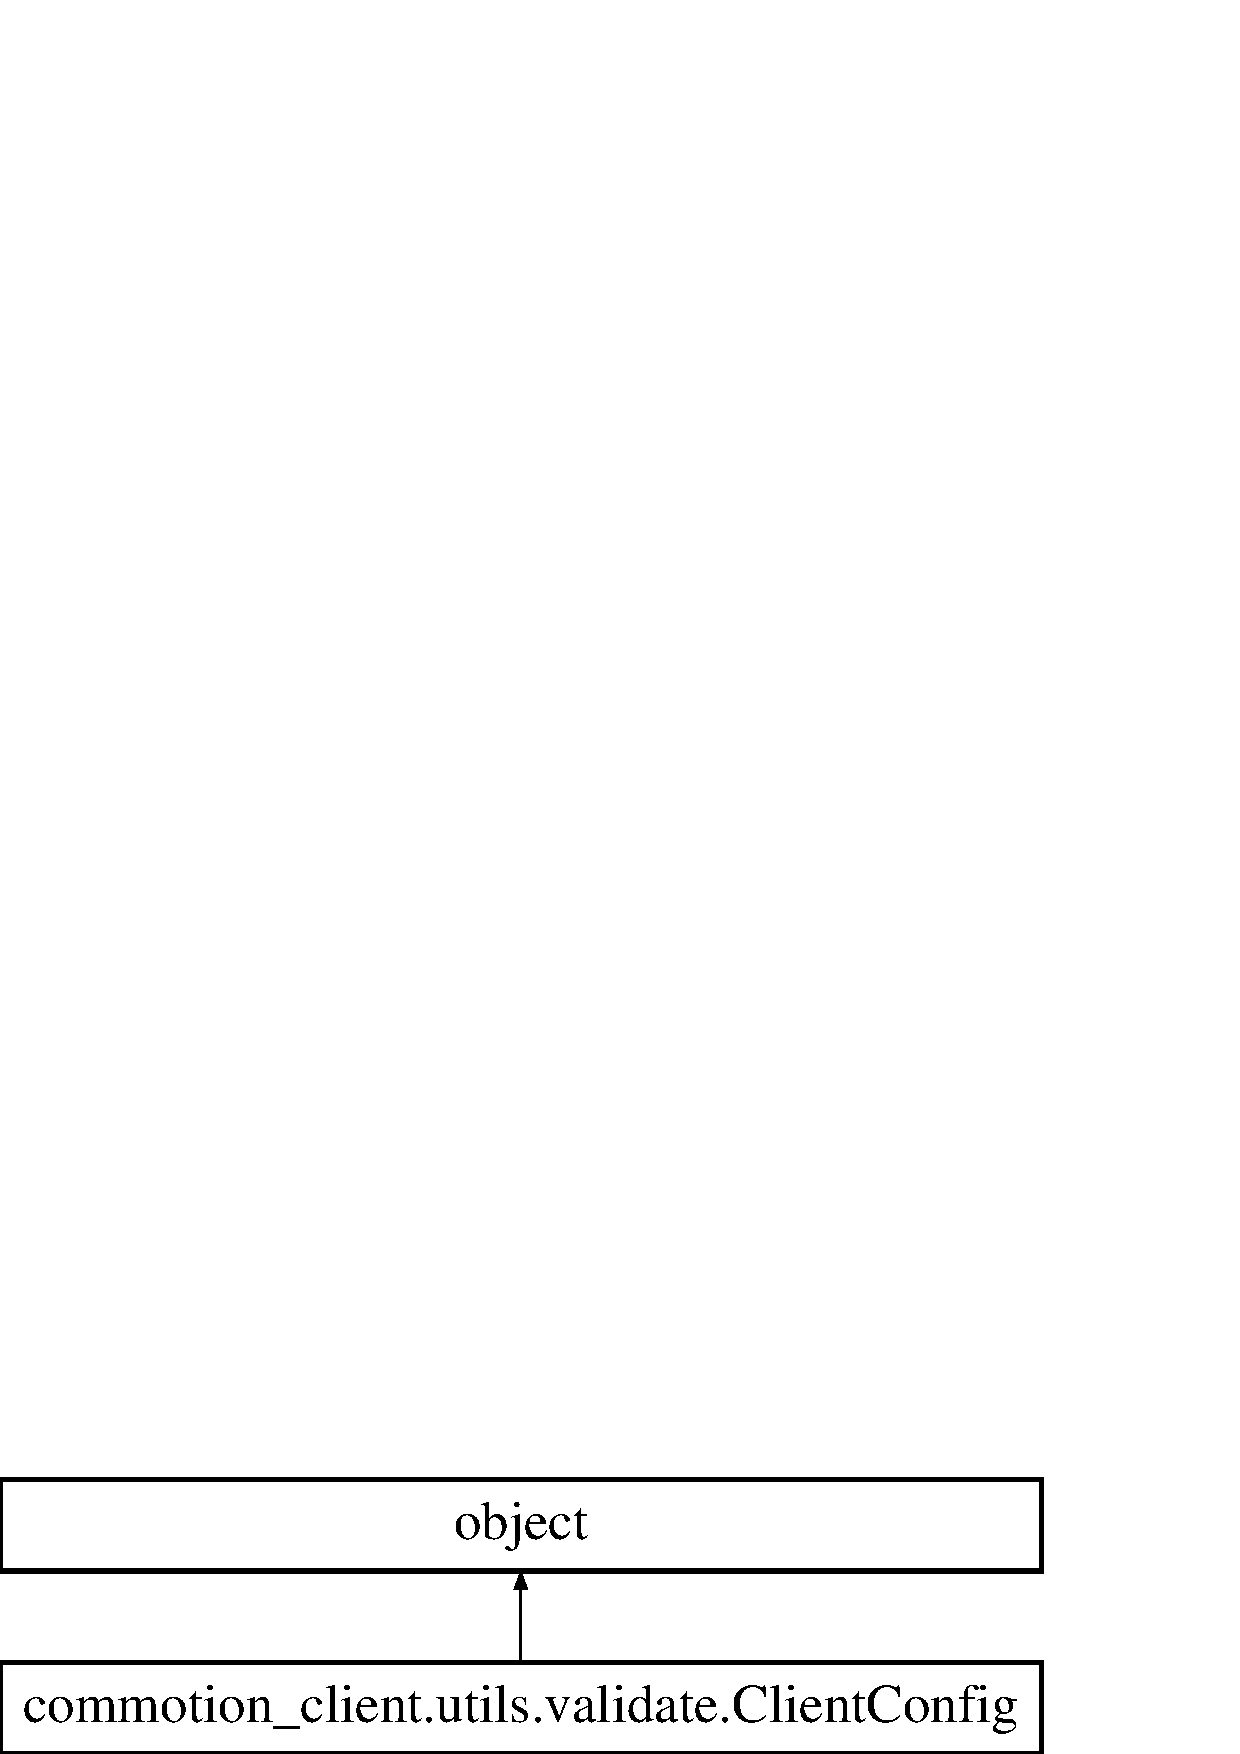
\includegraphics[height=2.000000cm]{classcommotion__client_1_1utils_1_1validate_1_1ClientConfig}
\end{center}
\end{figure}
\subsection*{Public Member Functions}
\begin{DoxyCompactItemize}
\item 
def \hyperlink{classcommotion__client_1_1utils_1_1validate_1_1ClientConfig_a1cf31ea11ff5dc7f47fcd62f16ab81f8}{\-\_\-\-\_\-init\-\_\-\-\_\-}
\item 
def \hyperlink{classcommotion__client_1_1utils_1_1validate_1_1ClientConfig_ad835c01a4478e52d1d4042e7230b0c61}{config}
\item 
def \hyperlink{classcommotion__client_1_1utils_1_1validate_1_1ClientConfig_ad835c01a4478e52d1d4042e7230b0c61}{config}
\item 
\hypertarget{classcommotion__client_1_1utils_1_1validate_1_1ClientConfig_a7e66cdad22581943cee6dae41cd5b84f}{def {\bfseries extension\-\_\-path}}\label{classcommotion__client_1_1utils_1_1validate_1_1ClientConfig_a7e66cdad22581943cee6dae41cd5b84f}

\item 
def \hyperlink{classcommotion__client_1_1utils_1_1validate_1_1ClientConfig_a7e66cdad22581943cee6dae41cd5b84f}{extension\-\_\-path}
\item 
def \hyperlink{classcommotion__client_1_1utils_1_1validate_1_1ClientConfig_ae1cfca31202df7ad46ca996cf9b38b3d}{validate\-\_\-all}
\item 
def \hyperlink{classcommotion__client_1_1utils_1_1validate_1_1ClientConfig_aa3a463fc48d9d7d219356d6150b4630f}{gui}
\item 
\hypertarget{classcommotion__client_1_1utils_1_1validate_1_1ClientConfig_ab92a3ae4cc66c3141e643792d05cab3c}{def {\bfseries name}}\label{classcommotion__client_1_1utils_1_1validate_1_1ClientConfig_ab92a3ae4cc66c3141e643792d05cab3c}

\item 
def \hyperlink{classcommotion__client_1_1utils_1_1validate_1_1ClientConfig_a1e7b94866f9c47f4e06c9ef4d9debcf8}{menu\-\_\-item}
\item 
def \hyperlink{classcommotion__client_1_1utils_1_1validate_1_1ClientConfig_ae7d3cc099ea0a5e7567473f13a8a3e86}{parent}
\item 
def \hyperlink{classcommotion__client_1_1utils_1_1validate_1_1ClientConfig_a811335c1b2495fd9ae46404ea748b5b1}{menu\-\_\-level}
\item 
def \hyperlink{classcommotion__client_1_1utils_1_1validate_1_1ClientConfig_a1e5b0345a6a5ad76e8f708982fb3ad99}{tests}
\item 
def \hyperlink{classcommotion__client_1_1utils_1_1validate_1_1ClientConfig_abd71aabe199cea9491c01afaa559e779}{check\-\_\-menu\-\_\-text}
\item 
def \hyperlink{classcommotion__client_1_1utils_1_1validate_1_1ClientConfig_a8dbef5da5fb270a8842b3eed36bc595e}{check\-\_\-exists}
\item 
def \hyperlink{classcommotion__client_1_1utils_1_1validate_1_1ClientConfig_a3564ac59723769f067537a4ff21aa027}{check\-\_\-path}
\item 
def \hyperlink{classcommotion__client_1_1utils_1_1validate_1_1ClientConfig_a2ca1bc57887049e8c5c8ce6a8a2b9eb7}{check\-\_\-path\-\_\-chars}
\item 
def \hyperlink{classcommotion__client_1_1utils_1_1validate_1_1ClientConfig_af89fc4407c4af2d96ad0146b1249a272}{check\-\_\-path\-\_\-length}
\end{DoxyCompactItemize}
\subsection*{Public Attributes}
\begin{DoxyCompactItemize}
\item 
\hypertarget{classcommotion__client_1_1utils_1_1validate_1_1ClientConfig_a2ef36c69221699da4e0fb2ccd47f50c1}{{\bfseries config\-\_\-values}}\label{classcommotion__client_1_1utils_1_1validate_1_1ClientConfig_a2ef36c69221699da4e0fb2ccd47f50c1}

\item 
\hypertarget{classcommotion__client_1_1utils_1_1validate_1_1ClientConfig_ac2b2577cf60d2fe5fee8e0d67f76d933}{{\bfseries log}}\label{classcommotion__client_1_1utils_1_1validate_1_1ClientConfig_ac2b2577cf60d2fe5fee8e0d67f76d933}

\item 
\hypertarget{classcommotion__client_1_1utils_1_1validate_1_1ClientConfig_a12d19377a853ce92cc0e0d758acdd804}{{\bfseries translate}}\label{classcommotion__client_1_1utils_1_1validate_1_1ClientConfig_a12d19377a853ce92cc0e0d758acdd804}

\item 
\hypertarget{classcommotion__client_1_1utils_1_1validate_1_1ClientConfig_acce323dd2fef1e3c2819cd0ed068cb67}{{\bfseries config}}\label{classcommotion__client_1_1utils_1_1validate_1_1ClientConfig_acce323dd2fef1e3c2819cd0ed068cb67}

\item 
\hypertarget{classcommotion__client_1_1utils_1_1validate_1_1ClientConfig_a422e4fea49a7e582749c0e0c6d11e2d9}{{\bfseries extension\-\_\-path}}\label{classcommotion__client_1_1utils_1_1validate_1_1ClientConfig_a422e4fea49a7e582749c0e0c6d11e2d9}

\item 
\hypertarget{classcommotion__client_1_1utils_1_1validate_1_1ClientConfig_ae3bf78ef12869745641fcf0fcd7f422f}{{\bfseries errors}}\label{classcommotion__client_1_1utils_1_1validate_1_1ClientConfig_ae3bf78ef12869745641fcf0fcd7f422f}

\end{DoxyCompactItemize}


\subsection{Constructor \& Destructor Documentation}
\hypertarget{classcommotion__client_1_1utils_1_1validate_1_1ClientConfig_a1cf31ea11ff5dc7f47fcd62f16ab81f8}{\index{commotion\-\_\-client\-::utils\-::validate\-::\-Client\-Config@{commotion\-\_\-client\-::utils\-::validate\-::\-Client\-Config}!\-\_\-\-\_\-init\-\_\-\-\_\-@{\-\_\-\-\_\-init\-\_\-\-\_\-}}
\index{\-\_\-\-\_\-init\-\_\-\-\_\-@{\-\_\-\-\_\-init\-\_\-\-\_\-}!commotion_client::utils::validate::ClientConfig@{commotion\-\_\-client\-::utils\-::validate\-::\-Client\-Config}}
\subsubsection[{\-\_\-\-\_\-init\-\_\-\-\_\-}]{\setlength{\rightskip}{0pt plus 5cm}def commotion\-\_\-client.\-utils.\-validate.\-Client\-Config.\-\_\-\-\_\-init\-\_\-\-\_\- (
\begin{DoxyParamCaption}
\item[{}]{self, }
\item[{}]{config, }
\item[{}]{directory = {\ttfamily None}}
\end{DoxyParamCaption}
)}}\label{classcommotion__client_1_1utils_1_1validate_1_1ClientConfig_a1cf31ea11ff5dc7f47fcd62f16ab81f8}
\begin{DoxyVerb}Args:
  config (dictionary): The config for the extension.
  directory (string): Absolute Path to the directory containing the extension zipfile. If not specified the validator will ONLY check the validity of the config passed to it.
\end{DoxyVerb}
 

References commotion\-\_\-client.\-utils.\-validate.\-Client\-Config.\-config, commotion\-\_\-client.\-utils.\-validate.\-Client\-Config.\-config\-\_\-values, commotion\-\_\-client.\-utils.\-validate.\-Client\-Config.\-errors, commotion\-\_\-client.\-utils.\-validate.\-Client\-Config.\-extension\-\_\-path, commotion\-\_\-client.\-G\-U\-I.\-system\-\_\-tray.\-Tray\-Icon.\-log, commotion\-\_\-client.\-utils.\-thread.\-Generic\-Thread.\-log, commotion\-\_\-client.\-utils.\-single\-\_\-application.\-Single\-Application.\-log, commotion\-\_\-client.\-G\-U\-I.\-welcome\-\_\-page.\-View\-Port.\-log, commotion\-\_\-client.\-G\-U\-I.\-menu\-\_\-bar.\-Menu\-Bar.\-log, commotion\-\_\-client.\-G\-U\-I.\-crash\-\_\-report.\-Crash\-Report.\-log, commotion\-\_\-client.\-extensions.\-config\-\_\-editor.\-main.\-View\-Port.\-log, commotion\-\_\-client.\-G\-U\-I.\-main\-\_\-window.\-Main\-Window.\-log, commotion\-\_\-client.\-G\-U\-I.\-toolbar\-\_\-builder.\-Tool\-Bar.\-log, commotion\-\_\-client.\-utils.\-validate.\-Client\-Config.\-log, commotion\-\_\-client.\-G\-U\-I.\-extension\-\_\-toolbar.\-Extension\-Tool\-Bar.\-log, commotion\-\_\-client.\-G\-U\-I.\-toolbar.\-Tool\-Bar.\-log, commotion\-\_\-client.\-utils.\-extension\-\_\-manager.\-Extension\-Manager.\-log, commotion\-\_\-client.\-commotion\-\_\-client.\-Hold\-State\-During\-Restart.\-log, commotion\-\_\-client.\-G\-U\-I.\-extension\-\_\-toolbar.\-Menu\-Item.\-log, commotion\-\_\-client.\-G\-U\-I.\-crash\-\_\-report.\-Report\-Gatherer.\-log, commotion\-\_\-client.\-commotion\-\_\-client.\-Commotion\-Client\-Application.\-log, commotion\-\_\-client.\-utils.\-extension\-\_\-manager.\-Config\-Manager.\-log, commotion\-\_\-client.\-G\-U\-I.\-menu\-\_\-bar.\-Menu\-Bar.\-translate, commotion\-\_\-client.\-extensions.\-config\-\_\-editor.\-main.\-View\-Port.\-translate, commotion\-\_\-client.\-G\-U\-I.\-main\-\_\-window.\-Main\-Window.\-translate, commotion\-\_\-client.\-G\-U\-I.\-toolbar\-\_\-builder.\-Tool\-Bar.\-translate, commotion\-\_\-client.\-G\-U\-I.\-toolbar.\-Tool\-Bar.\-translate, commotion\-\_\-client.\-G\-U\-I.\-extension\-\_\-toolbar.\-Extension\-Tool\-Bar.\-translate, commotion\-\_\-client.\-utils.\-validate.\-Client\-Config.\-translate, commotion\-\_\-client.\-utils.\-extension\-\_\-manager.\-Extension\-Manager.\-translate, commotion\-\_\-client.\-G\-U\-I.\-extension\-\_\-toolbar.\-Menu\-Item.\-translate, commotion\-\_\-client.\-commotion\-\_\-client.\-Commotion\-Client\-Application.\-translate, and commotion\-\_\-client.\-utils.\-extension\-\_\-manager.\-Config\-Manager.\-translate.


\begin{DoxyCode}
30 
31     \textcolor{keyword}{def }\hyperlink{classcommotion__client_1_1utils_1_1validate_1_1ClientConfig_a1cf31ea11ff5dc7f47fcd62f16ab81f8}{\_\_init\_\_}(self, config, directory=None):
32         \textcolor{stringliteral}{"""}
33 \textcolor{stringliteral}{        Args:}
34 \textcolor{stringliteral}{          config (dictionary): The config for the extension.}
35 \textcolor{stringliteral}{          directory (string): Absolute Path to the directory containing the extension zipfile. If not
       specified the validator will ONLY check the validity of the config passed to it.}
36 \textcolor{stringliteral}{        """}
37         self.\hyperlink{classcommotion__client_1_1utils_1_1validate_1_1ClientConfig_a2ef36c69221699da4e0fb2ccd47f50c1}{config\_values} = [\textcolor{stringliteral}{"name"},
38                               \textcolor{stringliteral}{"main"},
39                               \textcolor{stringliteral}{"menu\_item"},
40                               \textcolor{stringliteral}{"menu\_level"},
41                               \textcolor{stringliteral}{"parent"},
42                               \textcolor{stringliteral}{"settings"},
43                               \textcolor{stringliteral}{"toolbar"},
44                               \textcolor{stringliteral}{"tests"},
45                               \textcolor{stringliteral}{"initialized"},]
46         self.\hyperlink{classcommotion__client_1_1utils_1_1validate_1_1ClientConfig_ac2b2577cf60d2fe5fee8e0d67f76d933}{log} = logging.getLogger(\textcolor{stringliteral}{"commotion\_client."}+\_\_name\_\_)
47         self.\hyperlink{classcommotion__client_1_1utils_1_1validate_1_1ClientConfig_a12d19377a853ce92cc0e0d758acdd804}{translate} = QtCore.QCoreApplication.translate
48         self.\hyperlink{classcommotion__client_1_1utils_1_1validate_1_1ClientConfig_acce323dd2fef1e3c2819cd0ed068cb67}{config} = config
49         \textcolor{keywordflow}{if} directory:
50             \textcolor{comment}{#set extension directory to point at config zipfile in that directory}
51             self.\hyperlink{classcommotion__client_1_1utils_1_1validate_1_1ClientConfig_a422e4fea49a7e582749c0e0c6d11e2d9}{extension\_path} = directory
52         self.\hyperlink{classcommotion__client_1_1utils_1_1validate_1_1ClientConfig_ae3bf78ef12869745641fcf0fcd7f422f}{errors} = \textcolor{keywordtype}{None}

\end{DoxyCode}


\subsection{Member Function Documentation}
\hypertarget{classcommotion__client_1_1utils_1_1validate_1_1ClientConfig_a8dbef5da5fb270a8842b3eed36bc595e}{\index{commotion\-\_\-client\-::utils\-::validate\-::\-Client\-Config@{commotion\-\_\-client\-::utils\-::validate\-::\-Client\-Config}!check\-\_\-exists@{check\-\_\-exists}}
\index{check\-\_\-exists@{check\-\_\-exists}!commotion_client::utils::validate::ClientConfig@{commotion\-\_\-client\-::utils\-::validate\-::\-Client\-Config}}
\subsubsection[{check\-\_\-exists}]{\setlength{\rightskip}{0pt plus 5cm}def commotion\-\_\-client.\-utils.\-validate.\-Client\-Config.\-check\-\_\-exists (
\begin{DoxyParamCaption}
\item[{}]{self, }
\item[{}]{file\-\_\-name}
\end{DoxyParamCaption}
)}}\label{classcommotion__client_1_1utils_1_1validate_1_1ClientConfig_a8dbef5da5fb270a8842b3eed36bc595e}
\begin{DoxyVerb}Checks if a specified file exists within an extension.

@param file_name string The file name from a config file
\end{DoxyVerb}
 

References commotion\-\_\-client.\-utils.\-validate.\-Client\-Config.\-extension\-\_\-path, commotion\-\_\-client.\-G\-U\-I.\-menu\-\_\-bar.\-Menu\-Bar.\-translate, commotion\-\_\-client.\-extensions.\-config\-\_\-editor.\-main.\-View\-Port.\-translate, commotion\-\_\-client.\-G\-U\-I.\-main\-\_\-window.\-Main\-Window.\-translate, commotion\-\_\-client.\-G\-U\-I.\-toolbar\-\_\-builder.\-Tool\-Bar.\-translate, commotion\-\_\-client.\-G\-U\-I.\-toolbar.\-Tool\-Bar.\-translate, commotion\-\_\-client.\-G\-U\-I.\-extension\-\_\-toolbar.\-Extension\-Tool\-Bar.\-translate, commotion\-\_\-client.\-utils.\-validate.\-Client\-Config.\-translate, commotion\-\_\-client.\-utils.\-extension\-\_\-manager.\-Extension\-Manager.\-translate, commotion\-\_\-client.\-G\-U\-I.\-extension\-\_\-toolbar.\-Menu\-Item.\-translate, commotion\-\_\-client.\-commotion\-\_\-client.\-Commotion\-Client\-Application.\-translate, and commotion\-\_\-client.\-utils.\-extension\-\_\-manager.\-Config\-Manager.\-translate.



Referenced by commotion\-\_\-client.\-utils.\-validate.\-Client\-Config.\-gui(), and commotion\-\_\-client.\-utils.\-validate.\-Client\-Config.\-tests().


\begin{DoxyCode}
235 
236     \textcolor{keyword}{def }\hyperlink{classcommotion__client_1_1utils_1_1validate_1_1ClientConfig_a8dbef5da5fb270a8842b3eed36bc595e}{check\_exists}(self, file\_name):
237         \textcolor{stringliteral}{"""Checks if a specified file exists within an extension.}
238 \textcolor{stringliteral}{}
239 \textcolor{stringliteral}{        @param file\_name string The file name from a config file}
240 \textcolor{stringliteral}{        """}
241         \textcolor{keywordflow}{if} \textcolor{keywordflow}{not} self.\hyperlink{classcommotion__client_1_1utils_1_1validate_1_1ClientConfig_a422e4fea49a7e582749c0e0c6d11e2d9}{extension\_path}:
242             self.log.debug(self.\hyperlink{classcommotion__client_1_1utils_1_1validate_1_1ClientConfig_a12d19377a853ce92cc0e0d758acdd804}{translate}(\textcolor{stringliteral}{"logs"}, \textcolor{stringliteral}{"No extension directory was specified so file
       checking was skipped."}))
243             \textcolor{keywordflow}{return} \textcolor{keyword}{True}
244         ext\_zip = zipfile.ZipFile(self.\hyperlink{classcommotion__client_1_1utils_1_1validate_1_1ClientConfig_a422e4fea49a7e582749c0e0c6d11e2d9}{extension\_path}, \textcolor{stringliteral}{'}\textcolor{stringliteral}{r')}
245 \textcolor{stringliteral}{        files = ext\_zip.namelist()}
246 \textcolor{stringliteral}{        }\textcolor{keywordflow}{if} \textcolor{keywordflow}{not} str(file\_name) \textcolor{keywordflow}{in} files:
247             self.log.warning(self.\hyperlink{classcommotion__client_1_1utils_1_1validate_1_1ClientConfig_a12d19377a853ce92cc0e0d758acdd804}{translate}(\textcolor{stringliteral}{"logs"}, \textcolor{stringliteral}{"The specified file '\{0\}' does not exist."}.
      format(file\_name)))
248             \textcolor{keywordflow}{return} \textcolor{keyword}{False}
249         \textcolor{keywordflow}{else}:
250             \textcolor{keywordflow}{return} \textcolor{keyword}{True}
            
\end{DoxyCode}
\hypertarget{classcommotion__client_1_1utils_1_1validate_1_1ClientConfig_abd71aabe199cea9491c01afaa559e779}{\index{commotion\-\_\-client\-::utils\-::validate\-::\-Client\-Config@{commotion\-\_\-client\-::utils\-::validate\-::\-Client\-Config}!check\-\_\-menu\-\_\-text@{check\-\_\-menu\-\_\-text}}
\index{check\-\_\-menu\-\_\-text@{check\-\_\-menu\-\_\-text}!commotion_client::utils::validate::ClientConfig@{commotion\-\_\-client\-::utils\-::validate\-::\-Client\-Config}}
\subsubsection[{check\-\_\-menu\-\_\-text}]{\setlength{\rightskip}{0pt plus 5cm}def commotion\-\_\-client.\-utils.\-validate.\-Client\-Config.\-check\-\_\-menu\-\_\-text (
\begin{DoxyParamCaption}
\item[{}]{self, }
\item[{}]{menu\-\_\-text}
\end{DoxyParamCaption}
)}}\label{classcommotion__client_1_1utils_1_1validate_1_1ClientConfig_abd71aabe199cea9491c01afaa559e779}
\begin{DoxyVerb}Checks that menu text fits within the accepted string length bounds.

@param menu_text string The text that will appear in the menu.
\end{DoxyVerb}
 

References commotion\-\_\-client.\-G\-U\-I.\-menu\-\_\-bar.\-Menu\-Bar.\-translate, commotion\-\_\-client.\-extensions.\-config\-\_\-editor.\-main.\-View\-Port.\-translate, commotion\-\_\-client.\-G\-U\-I.\-main\-\_\-window.\-Main\-Window.\-translate, commotion\-\_\-client.\-G\-U\-I.\-toolbar\-\_\-builder.\-Tool\-Bar.\-translate, commotion\-\_\-client.\-utils.\-validate.\-Client\-Config.\-translate, commotion\-\_\-client.\-G\-U\-I.\-toolbar.\-Tool\-Bar.\-translate, commotion\-\_\-client.\-G\-U\-I.\-extension\-\_\-toolbar.\-Extension\-Tool\-Bar.\-translate, commotion\-\_\-client.\-utils.\-extension\-\_\-manager.\-Extension\-Manager.\-translate, commotion\-\_\-client.\-G\-U\-I.\-extension\-\_\-toolbar.\-Menu\-Item.\-translate, commotion\-\_\-client.\-commotion\-\_\-client.\-Commotion\-Client\-Application.\-translate, and commotion\-\_\-client.\-utils.\-extension\-\_\-manager.\-Config\-Manager.\-translate.



Referenced by commotion\-\_\-client.\-utils.\-validate.\-Client\-Config.\-menu\-\_\-item(), and commotion\-\_\-client.\-utils.\-validate.\-Client\-Config.\-parent().


\begin{DoxyCode}
223 
224     \textcolor{keyword}{def }\hyperlink{classcommotion__client_1_1utils_1_1validate_1_1ClientConfig_abd71aabe199cea9491c01afaa559e779}{check\_menu\_text}(self, menu\_text):
225         \textcolor{stringliteral}{"""}
226 \textcolor{stringliteral}{        Checks that menu text fits within the accepted string length bounds.}
227 \textcolor{stringliteral}{}
228 \textcolor{stringliteral}{        @param menu\_text string The text that will appear in the menu.}
229 \textcolor{stringliteral}{        """}
230         \textcolor{keywordflow}{if} \textcolor{keywordflow}{not} 3 < len(str(menu\_text)) < 40:
231             self.log.warning(self.\hyperlink{classcommotion__client_1_1utils_1_1validate_1_1ClientConfig_a12d19377a853ce92cc0e0d758acdd804}{translate}(\textcolor{stringliteral}{"logs"}, \textcolor{stringliteral}{"Menu items must be between 3 and 40 chars
       long. Becuase it looks prettier that way."}))
232             \textcolor{keywordflow}{return} \textcolor{keyword}{False}
233         \textcolor{keywordflow}{else}:
234             \textcolor{keywordflow}{return} \textcolor{keyword}{True}
            
\end{DoxyCode}
\hypertarget{classcommotion__client_1_1utils_1_1validate_1_1ClientConfig_a3564ac59723769f067537a4ff21aa027}{\index{commotion\-\_\-client\-::utils\-::validate\-::\-Client\-Config@{commotion\-\_\-client\-::utils\-::validate\-::\-Client\-Config}!check\-\_\-path@{check\-\_\-path}}
\index{check\-\_\-path@{check\-\_\-path}!commotion_client::utils::validate::ClientConfig@{commotion\-\_\-client\-::utils\-::validate\-::\-Client\-Config}}
\subsubsection[{check\-\_\-path}]{\setlength{\rightskip}{0pt plus 5cm}def commotion\-\_\-client.\-utils.\-validate.\-Client\-Config.\-check\-\_\-path (
\begin{DoxyParamCaption}
\item[{}]{self, }
\item[{}]{file\-\_\-name}
\end{DoxyParamCaption}
)}}\label{classcommotion__client_1_1utils_1_1validate_1_1ClientConfig_a3564ac59723769f067537a4ff21aa027}
\begin{DoxyVerb}Runs all path checking functions on a string.

@param file_name string  The string to check for validity.
\end{DoxyVerb}
 

References commotion\-\_\-client.\-utils.\-validate.\-Client\-Config.\-check\-\_\-path\-\_\-chars(), commotion\-\_\-client.\-utils.\-validate.\-Client\-Config.\-check\-\_\-path\-\_\-length(), commotion\-\_\-client.\-G\-U\-I.\-menu\-\_\-bar.\-Menu\-Bar.\-translate, commotion\-\_\-client.\-extensions.\-config\-\_\-editor.\-main.\-View\-Port.\-translate, commotion\-\_\-client.\-G\-U\-I.\-main\-\_\-window.\-Main\-Window.\-translate, commotion\-\_\-client.\-G\-U\-I.\-toolbar\-\_\-builder.\-Tool\-Bar.\-translate, commotion\-\_\-client.\-G\-U\-I.\-toolbar.\-Tool\-Bar.\-translate, commotion\-\_\-client.\-G\-U\-I.\-extension\-\_\-toolbar.\-Extension\-Tool\-Bar.\-translate, commotion\-\_\-client.\-utils.\-validate.\-Client\-Config.\-translate, commotion\-\_\-client.\-utils.\-extension\-\_\-manager.\-Extension\-Manager.\-translate, commotion\-\_\-client.\-G\-U\-I.\-extension\-\_\-toolbar.\-Menu\-Item.\-translate, commotion\-\_\-client.\-commotion\-\_\-client.\-Commotion\-Client\-Application.\-translate, and commotion\-\_\-client.\-utils.\-extension\-\_\-manager.\-Config\-Manager.\-translate.



Referenced by commotion\-\_\-client.\-utils.\-validate.\-Client\-Config.\-gui(), and commotion\-\_\-client.\-utils.\-validate.\-Client\-Config.\-tests().


\begin{DoxyCode}
251 
252     \textcolor{keyword}{def }\hyperlink{classcommotion__client_1_1utils_1_1validate_1_1ClientConfig_a3564ac59723769f067537a4ff21aa027}{check\_path}(self, file\_name):
253         \textcolor{stringliteral}{"""Runs all path checking functions on a string.}
254 \textcolor{stringliteral}{}
255 \textcolor{stringliteral}{        @param file\_name string  The string to check for validity.}
256 \textcolor{stringliteral}{        """}
257         \textcolor{keywordflow}{if} \textcolor{keywordflow}{not} self.\hyperlink{classcommotion__client_1_1utils_1_1validate_1_1ClientConfig_af89fc4407c4af2d96ad0146b1249a272}{check\_path\_length}(file\_name):
258             self.log.warning(self.\hyperlink{classcommotion__client_1_1utils_1_1validate_1_1ClientConfig_a12d19377a853ce92cc0e0d758acdd804}{translate}(\textcolor{stringliteral}{"logs"}, \textcolor{stringliteral}{"This value is too long for your system."}))
259             \textcolor{keywordflow}{return} \textcolor{keyword}{False}
260         \textcolor{keywordflow}{if} \textcolor{keywordflow}{not} self.\hyperlink{classcommotion__client_1_1utils_1_1validate_1_1ClientConfig_a2ca1bc57887049e8c5c8ce6a8a2b9eb7}{check\_path\_chars}(file\_name):
261             self.log.warning(self.\hyperlink{classcommotion__client_1_1utils_1_1validate_1_1ClientConfig_a12d19377a853ce92cc0e0d758acdd804}{translate}(\textcolor{stringliteral}{"logs"}, \textcolor{stringliteral}{"This value uses invalid characters for your
       system."}))
262             \textcolor{keywordflow}{return} \textcolor{keyword}{False}
263         \textcolor{keywordflow}{return} \textcolor{keyword}{True}

\end{DoxyCode}
\hypertarget{classcommotion__client_1_1utils_1_1validate_1_1ClientConfig_a2ca1bc57887049e8c5c8ce6a8a2b9eb7}{\index{commotion\-\_\-client\-::utils\-::validate\-::\-Client\-Config@{commotion\-\_\-client\-::utils\-::validate\-::\-Client\-Config}!check\-\_\-path\-\_\-chars@{check\-\_\-path\-\_\-chars}}
\index{check\-\_\-path\-\_\-chars@{check\-\_\-path\-\_\-chars}!commotion_client::utils::validate::ClientConfig@{commotion\-\_\-client\-::utils\-::validate\-::\-Client\-Config}}
\subsubsection[{check\-\_\-path\-\_\-chars}]{\setlength{\rightskip}{0pt plus 5cm}def commotion\-\_\-client.\-utils.\-validate.\-Client\-Config.\-check\-\_\-path\-\_\-chars (
\begin{DoxyParamCaption}
\item[{}]{self, }
\item[{}]{file\-\_\-name}
\end{DoxyParamCaption}
)}}\label{classcommotion__client_1_1utils_1_1validate_1_1ClientConfig_a2ca1bc57887049e8c5c8ce6a8a2b9eb7}
\begin{DoxyVerb}Checks if a string is a valid file name on this system.

@param file_name string The string to check for validity
\end{DoxyVerb}
 

References commotion\-\_\-client.\-G\-U\-I.\-menu\-\_\-bar.\-Menu\-Bar.\-translate, commotion\-\_\-client.\-extensions.\-config\-\_\-editor.\-main.\-View\-Port.\-translate, commotion\-\_\-client.\-G\-U\-I.\-main\-\_\-window.\-Main\-Window.\-translate, commotion\-\_\-client.\-G\-U\-I.\-toolbar\-\_\-builder.\-Tool\-Bar.\-translate, commotion\-\_\-client.\-utils.\-validate.\-Client\-Config.\-translate, commotion\-\_\-client.\-G\-U\-I.\-toolbar.\-Tool\-Bar.\-translate, commotion\-\_\-client.\-G\-U\-I.\-extension\-\_\-toolbar.\-Extension\-Tool\-Bar.\-translate, commotion\-\_\-client.\-utils.\-extension\-\_\-manager.\-Extension\-Manager.\-translate, commotion\-\_\-client.\-G\-U\-I.\-extension\-\_\-toolbar.\-Menu\-Item.\-translate, commotion\-\_\-client.\-commotion\-\_\-client.\-Commotion\-Client\-Application.\-translate, and commotion\-\_\-client.\-utils.\-extension\-\_\-manager.\-Config\-Manager.\-translate.



Referenced by commotion\-\_\-client.\-utils.\-validate.\-Client\-Config.\-check\-\_\-path(), and commotion\-\_\-client.\-utils.\-validate.\-Client\-Config.\-gui().


\begin{DoxyCode}
264 
265     \textcolor{keyword}{def }\hyperlink{classcommotion__client_1_1utils_1_1validate_1_1ClientConfig_a2ca1bc57887049e8c5c8ce6a8a2b9eb7}{check\_path\_chars}(self, file\_name):
266         \textcolor{stringliteral}{"""Checks if a string is a valid file name on this system.}
267 \textcolor{stringliteral}{}
268 \textcolor{stringliteral}{        @param file\_name string The string to check for validity}
269 \textcolor{stringliteral}{        """}
270         \textcolor{comment}{# file length limit}
271         platform = sys.platform
272         reserved = \{\textcolor{stringliteral}{"cygwin"} : \textcolor{stringliteral}{r"[|\(\backslash\)?*<\(\backslash\)":>+[]/]"},
273                     \textcolor{stringliteral}{"win32"} : \textcolor{stringliteral}{r"[|\(\backslash\)?*<\(\backslash\)":>+[]/]"},
274                     \textcolor{stringliteral}{"darwin"} : \textcolor{stringliteral}{"[:]"},
275                     \textcolor{stringliteral}{"linux"} : \textcolor{stringliteral}{"[/\(\backslash\)x00]"}\}
276         \textcolor{keywordflow}{if} platform \textcolor{keywordflow}{and} reserved[platform]:
277             \textcolor{keywordflow}{if} re.search(file\_name, reserved[platform]):
278                 self.log.warning(self.\hyperlink{classcommotion__client_1_1utils_1_1validate_1_1ClientConfig_a12d19377a853ce92cc0e0d758acdd804}{translate}(\textcolor{stringliteral}{"logs"}, \textcolor{stringliteral}{"The extension's config file contains an
       invalid main value."}))
279                 \textcolor{keywordflow}{return} \textcolor{keyword}{False}
280             \textcolor{keywordflow}{else}:
281                 \textcolor{keywordflow}{return} \textcolor{keyword}{True}
282         \textcolor{keywordflow}{else}:
283             self.log.warning(self.\hyperlink{classcommotion__client_1_1utils_1_1validate_1_1ClientConfig_a12d19377a853ce92cc0e0d758acdd804}{translate}(\textcolor{stringliteral}{"logs"}, \textcolor{stringliteral}{"Your system, \{0\} is not recognized. This may
       cause instability if file uses chars that your system does not allow."}).format(platform))
284             \textcolor{keywordflow}{return} \textcolor{keyword}{True}
285                 
            
\end{DoxyCode}
\hypertarget{classcommotion__client_1_1utils_1_1validate_1_1ClientConfig_af89fc4407c4af2d96ad0146b1249a272}{\index{commotion\-\_\-client\-::utils\-::validate\-::\-Client\-Config@{commotion\-\_\-client\-::utils\-::validate\-::\-Client\-Config}!check\-\_\-path\-\_\-length@{check\-\_\-path\-\_\-length}}
\index{check\-\_\-path\-\_\-length@{check\-\_\-path\-\_\-length}!commotion_client::utils::validate::ClientConfig@{commotion\-\_\-client\-::utils\-::validate\-::\-Client\-Config}}
\subsubsection[{check\-\_\-path\-\_\-length}]{\setlength{\rightskip}{0pt plus 5cm}def commotion\-\_\-client.\-utils.\-validate.\-Client\-Config.\-check\-\_\-path\-\_\-length (
\begin{DoxyParamCaption}
\item[{}]{self, }
\item[{}]{file\-\_\-name = {\ttfamily None}}
\end{DoxyParamCaption}
)}}\label{classcommotion__client_1_1utils_1_1validate_1_1ClientConfig_af89fc4407c4af2d96ad0146b1249a272}
\begin{DoxyVerb}Checks if a string will be of a valid length for a file name and full path on this system.

@param file_name string The string to check for validity.
\end{DoxyVerb}
 

References commotion\-\_\-client.\-utils.\-validate.\-Client\-Config.\-extension\-\_\-path, commotion\-\_\-client.\-G\-U\-I.\-menu\-\_\-bar.\-Menu\-Bar.\-translate, commotion\-\_\-client.\-extensions.\-config\-\_\-editor.\-main.\-View\-Port.\-translate, commotion\-\_\-client.\-G\-U\-I.\-main\-\_\-window.\-Main\-Window.\-translate, commotion\-\_\-client.\-G\-U\-I.\-toolbar\-\_\-builder.\-Tool\-Bar.\-translate, commotion\-\_\-client.\-G\-U\-I.\-toolbar.\-Tool\-Bar.\-translate, commotion\-\_\-client.\-G\-U\-I.\-extension\-\_\-toolbar.\-Extension\-Tool\-Bar.\-translate, commotion\-\_\-client.\-utils.\-validate.\-Client\-Config.\-translate, commotion\-\_\-client.\-utils.\-extension\-\_\-manager.\-Extension\-Manager.\-translate, commotion\-\_\-client.\-G\-U\-I.\-extension\-\_\-toolbar.\-Menu\-Item.\-translate, commotion\-\_\-client.\-commotion\-\_\-client.\-Commotion\-Client\-Application.\-translate, and commotion\-\_\-client.\-utils.\-extension\-\_\-manager.\-Config\-Manager.\-translate.



Referenced by commotion\-\_\-client.\-utils.\-validate.\-Client\-Config.\-check\-\_\-path(), and commotion\-\_\-client.\-utils.\-validate.\-Client\-Config.\-gui().


\begin{DoxyCode}
286 
287     \textcolor{keyword}{def }\hyperlink{classcommotion__client_1_1utils_1_1validate_1_1ClientConfig_af89fc4407c4af2d96ad0146b1249a272}{check\_path\_length}(self, file\_name=None):
288         \textcolor{stringliteral}{"""Checks if a string will be of a valid length for a file name and full path on this system.}
289 \textcolor{stringliteral}{}
290 \textcolor{stringliteral}{        @param file\_name string The string to check for validity.}
291 \textcolor{stringliteral}{        """}
292         \textcolor{keywordflow}{if} \textcolor{keywordflow}{not} self.\hyperlink{classcommotion__client_1_1utils_1_1validate_1_1ClientConfig_a422e4fea49a7e582749c0e0c6d11e2d9}{extension\_path}:
293             self.log.debug(self.\hyperlink{classcommotion__client_1_1utils_1_1validate_1_1ClientConfig_a12d19377a853ce92cc0e0d758acdd804}{translate}(\textcolor{stringliteral}{"logs"}, \textcolor{stringliteral}{"No extension directory was specified so file
       checking was skipped."}))
294             \textcolor{keywordflow}{return} \textcolor{keyword}{True}
295         \textcolor{comment}{# file length limit}
296         platform = sys.platform
297         \textcolor{comment}{# OSX(name<=255),  linux(name<=255)}
298         name\_limit = [\textcolor{stringliteral}{'linux'}, \textcolor{stringliteral}{'darwin'}]
299         \textcolor{comment}{# Win(name+path<=260),}
300         path\_limit = [\textcolor{stringliteral}{'win32'}, \textcolor{stringliteral}{'cygwin'}]
301         \textcolor{keywordflow}{if} platform \textcolor{keywordflow}{in} path\_limit:
302             extension\_path = os.path.join(QtCore.QDir.currentPath(), \textcolor{stringliteral}{"extensions"})
303             full\_path = os.path.join(extension\_path, file\_name)
304             \textcolor{keywordflow}{if} len(str(full\_path)) > 255:
305                 self.log.warning(self.\hyperlink{classcommotion__client_1_1utils_1_1validate_1_1ClientConfig_a12d19377a853ce92cc0e0d758acdd804}{translate}(\textcolor{stringliteral}{"logs"}, \textcolor{stringliteral}{"The full extension path cannot be greater
       than 260 chars"}))
306                 \textcolor{keywordflow}{return} \textcolor{keyword}{False}
307             \textcolor{keywordflow}{else}:
308                 \textcolor{keywordflow}{return} \textcolor{keyword}{True}
309         \textcolor{keywordflow}{elif} platform \textcolor{keywordflow}{in} name\_limit:
310             \textcolor{keywordflow}{if} len(str(file\_name)) >= 260:
311                 self.log.warning(self.\hyperlink{classcommotion__client_1_1utils_1_1validate_1_1ClientConfig_a12d19377a853ce92cc0e0d758acdd804}{translate}(\textcolor{stringliteral}{"logs"}, \textcolor{stringliteral}{"File names can not be greater than 260
       chars on your system"}))
312                 \textcolor{keywordflow}{return} \textcolor{keyword}{False}
313             \textcolor{keywordflow}{else}:
314                 \textcolor{keywordflow}{return} \textcolor{keyword}{True}
315         \textcolor{keywordflow}{else}:
316             self.log.warning(self.\hyperlink{classcommotion__client_1_1utils_1_1validate_1_1ClientConfig_a12d19377a853ce92cc0e0d758acdd804}{translate}(\textcolor{stringliteral}{"logs"}, \textcolor{stringliteral}{"Your system, \{0\} is not recognized. This may
       cause instability if file or path names are longer than your system allows."}).format(platform))
317             \textcolor{keywordflow}{return} \textcolor{keyword}{True}

\end{DoxyCode}
\hypertarget{classcommotion__client_1_1utils_1_1validate_1_1ClientConfig_ad835c01a4478e52d1d4042e7230b0c61}{\index{commotion\-\_\-client\-::utils\-::validate\-::\-Client\-Config@{commotion\-\_\-client\-::utils\-::validate\-::\-Client\-Config}!config@{config}}
\index{config@{config}!commotion_client::utils::validate::ClientConfig@{commotion\-\_\-client\-::utils\-::validate\-::\-Client\-Config}}
\subsubsection[{config}]{\setlength{\rightskip}{0pt plus 5cm}def commotion\-\_\-client.\-utils.\-validate.\-Client\-Config.\-config (
\begin{DoxyParamCaption}
\item[{}]{self}
\end{DoxyParamCaption}
)}}\label{classcommotion__client_1_1utils_1_1validate_1_1ClientConfig_ad835c01a4478e52d1d4042e7230b0c61}
\begin{DoxyVerb}Return the config value.\end{DoxyVerb}
 

References commotion\-\_\-client.\-utils.\-validate.\-Client\-Config.\-\_\-config.


\begin{DoxyCode}
54 
55     \textcolor{keyword}{def }config(self):
56         \textcolor{stringliteral}{"""Return the config value."""}
57         \textcolor{keywordflow}{return} self.\hyperlink{classcommotion__client_1_1utils_1_1validate_1_1ClientConfig_ad0ab5b07ecdef6225318bbc0cb711381}{\_config}

\end{DoxyCode}
\hypertarget{classcommotion__client_1_1utils_1_1validate_1_1ClientConfig_ad835c01a4478e52d1d4042e7230b0c61}{\index{commotion\-\_\-client\-::utils\-::validate\-::\-Client\-Config@{commotion\-\_\-client\-::utils\-::validate\-::\-Client\-Config}!config@{config}}
\index{config@{config}!commotion_client::utils::validate::ClientConfig@{commotion\-\_\-client\-::utils\-::validate\-::\-Client\-Config}}
\subsubsection[{config}]{\setlength{\rightskip}{0pt plus 5cm}def commotion\-\_\-client.\-utils.\-validate.\-Client\-Config.\-config (
\begin{DoxyParamCaption}
\item[{}]{self, }
\item[{}]{value}
\end{DoxyParamCaption}
)}}\label{classcommotion__client_1_1utils_1_1validate_1_1ClientConfig_ad835c01a4478e52d1d4042e7230b0c61}
\begin{DoxyVerb}Check for valid values before allowing them to be set.\end{DoxyVerb}
 

References commotion\-\_\-client.\-utils.\-validate.\-Client\-Config.\-\_\-config, commotion\-\_\-client.\-utils.\-validate.\-Client\-Config.\-\_\-extension\-\_\-path, commotion\-\_\-client.\-utils.\-validate.\-Client\-Config.\-config\-\_\-values, commotion\-\_\-client.\-G\-U\-I.\-menu\-\_\-bar.\-Menu\-Bar.\-translate, commotion\-\_\-client.\-extensions.\-config\-\_\-editor.\-main.\-View\-Port.\-translate, commotion\-\_\-client.\-G\-U\-I.\-main\-\_\-window.\-Main\-Window.\-translate, commotion\-\_\-client.\-G\-U\-I.\-toolbar\-\_\-builder.\-Tool\-Bar.\-translate, commotion\-\_\-client.\-utils.\-validate.\-Client\-Config.\-translate, commotion\-\_\-client.\-G\-U\-I.\-toolbar.\-Tool\-Bar.\-translate, commotion\-\_\-client.\-G\-U\-I.\-extension\-\_\-toolbar.\-Extension\-Tool\-Bar.\-translate, commotion\-\_\-client.\-utils.\-extension\-\_\-manager.\-Extension\-Manager.\-translate, commotion\-\_\-client.\-G\-U\-I.\-extension\-\_\-toolbar.\-Menu\-Item.\-translate, commotion\-\_\-client.\-commotion\-\_\-client.\-Commotion\-Client\-Application.\-translate, and commotion\-\_\-client.\-utils.\-extension\-\_\-manager.\-Config\-Manager.\-translate.


\begin{DoxyCode}
59 
60     \textcolor{keyword}{def }config(self, value):
61         \textcolor{stringliteral}{"""Check for valid values before allowing them to be set."""}
62         \textcolor{keywordflow}{if} \textcolor{stringliteral}{'name'} \textcolor{keywordflow}{not} \textcolor{keywordflow}{in} value:
63             \textcolor{keywordflow}{raise} KeyError(self.\hyperlink{classcommotion__client_1_1utils_1_1validate_1_1ClientConfig_a12d19377a853ce92cc0e0d758acdd804}{translate}(\textcolor{stringliteral}{"logs"}, \textcolor{stringliteral}{"The config file must contain at least a name
       value."}))
64         \textcolor{keywordflow}{for} val \textcolor{keywordflow}{in} value.keys():
65             \textcolor{keywordflow}{if} val \textcolor{keywordflow}{not} \textcolor{keywordflow}{in} self.\hyperlink{classcommotion__client_1_1utils_1_1validate_1_1ClientConfig_a2ef36c69221699da4e0fb2ccd47f50c1}{config\_values}:
66                 \textcolor{keywordflow}{raise} KeyError(self.\hyperlink{classcommotion__client_1_1utils_1_1validate_1_1ClientConfig_a12d19377a853ce92cc0e0d758acdd804}{translate}(\textcolor{stringliteral}{"logs"}, \textcolor{stringliteral}{"The config file specified has the value \{0\}
       within it which is not a valid value."}.format(val)))
67         self.\hyperlink{classcommotion__client_1_1utils_1_1validate_1_1ClientConfig_ad0ab5b07ecdef6225318bbc0cb711381}{\_config} = value
68                                      

\end{DoxyCode}
\hypertarget{classcommotion__client_1_1utils_1_1validate_1_1ClientConfig_a7e66cdad22581943cee6dae41cd5b84f}{\index{commotion\-\_\-client\-::utils\-::validate\-::\-Client\-Config@{commotion\-\_\-client\-::utils\-::validate\-::\-Client\-Config}!extension\-\_\-path@{extension\-\_\-path}}
\index{extension\-\_\-path@{extension\-\_\-path}!commotion_client::utils::validate::ClientConfig@{commotion\-\_\-client\-::utils\-::validate\-::\-Client\-Config}}
\subsubsection[{extension\-\_\-path}]{\setlength{\rightskip}{0pt plus 5cm}def commotion\-\_\-client.\-utils.\-validate.\-Client\-Config.\-extension\-\_\-path (
\begin{DoxyParamCaption}
\item[{}]{self, }
\item[{}]{value}
\end{DoxyParamCaption}
)}}\label{classcommotion__client_1_1utils_1_1validate_1_1ClientConfig_a7e66cdad22581943cee6dae41cd5b84f}
\begin{DoxyVerb}Takes any directory passed to it and specifies the config file  \end{DoxyVerb}
 

References commotion\-\_\-client.\-utils.\-validate.\-Client\-Config.\-\_\-extension\-\_\-path, commotion\-\_\-client.\-utils.\-validate.\-Client\-Config.\-config, commotion\-\_\-client.\-G\-U\-I.\-menu\-\_\-bar.\-Menu\-Bar.\-translate, commotion\-\_\-client.\-extensions.\-config\-\_\-editor.\-main.\-View\-Port.\-translate, commotion\-\_\-client.\-G\-U\-I.\-main\-\_\-window.\-Main\-Window.\-translate, commotion\-\_\-client.\-G\-U\-I.\-toolbar\-\_\-builder.\-Tool\-Bar.\-translate, commotion\-\_\-client.\-utils.\-validate.\-Client\-Config.\-translate, commotion\-\_\-client.\-G\-U\-I.\-toolbar.\-Tool\-Bar.\-translate, commotion\-\_\-client.\-G\-U\-I.\-extension\-\_\-toolbar.\-Extension\-Tool\-Bar.\-translate, commotion\-\_\-client.\-utils.\-extension\-\_\-manager.\-Extension\-Manager.\-translate, commotion\-\_\-client.\-G\-U\-I.\-extension\-\_\-toolbar.\-Menu\-Item.\-translate, commotion\-\_\-client.\-commotion\-\_\-client.\-Commotion\-Client\-Application.\-translate, and commotion\-\_\-client.\-utils.\-extension\-\_\-manager.\-Config\-Manager.\-translate.


\begin{DoxyCode}
74 
75     \textcolor{keyword}{def }extension\_path(self, value):
76         \textcolor{stringliteral}{"""Takes any directory passed to it and specifies the config file  """}
77         value\_dir = QtCore.QDir(value)
78         \textcolor{comment}{#Check that the directory in fact exists.}
79         \textcolor{keywordflow}{if} \textcolor{keywordflow}{not} value\_dir.exists():
80             \textcolor{keywordflow}{raise} NotADirectoryError(self.\hyperlink{classcommotion__client_1_1utils_1_1validate_1_1ClientConfig_a12d19377a853ce92cc0e0d758acdd804}{translate}(\textcolor{stringliteral}{"logs"}, \textcolor{stringliteral}{"The directory should, by definition,
       actually be a directory. What was submitted was not a directory. Please specify the directory of an existing
       extension to continue."}))
81         \textcolor{comment}{#Check that there are files in the directory provided}
82         \textcolor{keywordflow}{if} \textcolor{keywordflow}{not} value\_dir.exists(self.\hyperlink{classcommotion__client_1_1utils_1_1validate_1_1ClientConfig_acce323dd2fef1e3c2819cd0ed068cb67}{config}[\textcolor{stringliteral}{'name'}]):
83             \textcolor{keywordflow}{raise} FileNotFoundError(self.\hyperlink{classcommotion__client_1_1utils_1_1validate_1_1ClientConfig_a12d19377a853ce92cc0e0d758acdd804}{translate}(\textcolor{stringliteral}{"logs"}, \textcolor{stringliteral}{"The extension is not in the extension
       directory provided. Is an extension directory without an extension an extension directory at all? We will
       ponder these mysteries while you check to see if the extension directory provided is correct."} ))
84         \textcolor{comment}{#Check that we can read the directory and its files. Sadly, QDir.isReadable() is broken on a few
       platforms so we check that and use the file filter to check each file.}
85         value\_dir.setFilter(QtCore.QDir.Readable|QtCore.QDir.Files)
86         file\_list = value\_dir.entryInfoList()
87         \textcolor{keywordflow}{if} \textcolor{keywordflow}{not} file\_list \textcolor{keywordflow}{or} \textcolor{keywordflow}{not} value\_dir.isReadable():
88             \textcolor{keywordflow}{raise} PermissionError(self.\hyperlink{classcommotion__client_1_1utils_1_1validate_1_1ClientConfig_a12d19377a853ce92cc0e0d758acdd804}{translate}(\textcolor{stringliteral}{"logs"}, \textcolor{stringliteral}{"The application does not have permission
       to read any files within this directory. How is it supposed to validate the extension within then? You ask.
       It can't. Please modify the permissions on the directory and files within to allow the application to read
       the extension file."}))
89         \textcolor{comment}{#Set the extension "directory" to point at the extension zipfile}
90         path = os.path.join(value, self.\hyperlink{classcommotion__client_1_1utils_1_1validate_1_1ClientConfig_acce323dd2fef1e3c2819cd0ed068cb67}{config}[\textcolor{stringliteral}{'name'}])
91         self.\hyperlink{classcommotion__client_1_1utils_1_1validate_1_1ClientConfig_a42238419ef470bda7d663cea34c74213}{\_extension\_path} = path

\end{DoxyCode}
\hypertarget{classcommotion__client_1_1utils_1_1validate_1_1ClientConfig_aa3a463fc48d9d7d219356d6150b4630f}{\index{commotion\-\_\-client\-::utils\-::validate\-::\-Client\-Config@{commotion\-\_\-client\-::utils\-::validate\-::\-Client\-Config}!gui@{gui}}
\index{gui@{gui}!commotion_client::utils::validate::ClientConfig@{commotion\-\_\-client\-::utils\-::validate\-::\-Client\-Config}}
\subsubsection[{gui}]{\setlength{\rightskip}{0pt plus 5cm}def commotion\-\_\-client.\-utils.\-validate.\-Client\-Config.\-gui (
\begin{DoxyParamCaption}
\item[{}]{self, }
\item[{}]{gui\-\_\-name}
\end{DoxyParamCaption}
)}}\label{classcommotion__client_1_1utils_1_1validate_1_1ClientConfig_aa3a463fc48d9d7d219356d6150b4630f}
\begin{DoxyVerb}Validate of one of the gui objects config values. (main, settings, or toolbar)

@param gui_name string "main", "settings", or "toolbar"
\end{DoxyVerb}
 

References commotion\-\_\-client.\-utils.\-validate.\-Client\-Config.\-check\-\_\-exists(), commotion\-\_\-client.\-utils.\-validate.\-Client\-Config.\-check\-\_\-path(), commotion\-\_\-client.\-utils.\-validate.\-Client\-Config.\-check\-\_\-path\-\_\-chars(), commotion\-\_\-client.\-utils.\-validate.\-Client\-Config.\-check\-\_\-path\-\_\-length(), commotion\-\_\-client.\-utils.\-validate.\-Client\-Config.\-config, commotion\-\_\-client.\-G\-U\-I.\-menu\-\_\-bar.\-Menu\-Bar.\-translate, commotion\-\_\-client.\-extensions.\-config\-\_\-editor.\-main.\-View\-Port.\-translate, commotion\-\_\-client.\-G\-U\-I.\-main\-\_\-window.\-Main\-Window.\-translate, commotion\-\_\-client.\-G\-U\-I.\-toolbar\-\_\-builder.\-Tool\-Bar.\-translate, commotion\-\_\-client.\-G\-U\-I.\-toolbar.\-Tool\-Bar.\-translate, commotion\-\_\-client.\-G\-U\-I.\-extension\-\_\-toolbar.\-Extension\-Tool\-Bar.\-translate, commotion\-\_\-client.\-utils.\-validate.\-Client\-Config.\-translate, commotion\-\_\-client.\-utils.\-extension\-\_\-manager.\-Extension\-Manager.\-translate, commotion\-\_\-client.\-G\-U\-I.\-extension\-\_\-toolbar.\-Menu\-Item.\-translate, commotion\-\_\-client.\-commotion\-\_\-client.\-Commotion\-Client\-Application.\-translate, and commotion\-\_\-client.\-utils.\-extension\-\_\-manager.\-Config\-Manager.\-translate.



Referenced by commotion\-\_\-client.\-utils.\-validate.\-Client\-Config.\-validate\-\_\-all().


\begin{DoxyCode}
129 
130     \textcolor{keyword}{def }\hyperlink{classcommotion__client_1_1utils_1_1validate_1_1ClientConfig_aa3a463fc48d9d7d219356d6150b4630f}{gui}(self, gui\_name):
131         \textcolor{stringliteral}{"""Validate of one of the gui objects config values. (main, settings, or toolbar)}
132 \textcolor{stringliteral}{}
133 \textcolor{stringliteral}{        @param gui\_name string "main", "settings", or "toolbar"}
134 \textcolor{stringliteral}{        """}
135         \textcolor{keywordflow}{try}:
136             val = str(self.\hyperlink{classcommotion__client_1_1utils_1_1validate_1_1ClientConfig_acce323dd2fef1e3c2819cd0ed068cb67}{config}[gui\_name])
137         \textcolor{keywordflow}{except} KeyError:
138             \textcolor{keywordflow}{if} gui\_name != \textcolor{stringliteral}{"main"}:
139                 \textcolor{keywordflow}{try}:
140                     val = str(self.\hyperlink{classcommotion__client_1_1utils_1_1validate_1_1ClientConfig_acce323dd2fef1e3c2819cd0ed068cb67}{config}[\textcolor{stringliteral}{"main"}])
141                 \textcolor{keywordflow}{except} KeyError:
142                     val = str(\textcolor{stringliteral}{'main'})
143             \textcolor{keywordflow}{else}:
144                 val = str(\textcolor{stringliteral}{'main'})
145         file\_name = val + \textcolor{stringliteral}{".py"}
146         \textcolor{keywordflow}{if} \textcolor{keywordflow}{not} self.\hyperlink{classcommotion__client_1_1utils_1_1validate_1_1ClientConfig_a3564ac59723769f067537a4ff21aa027}{check\_path}(file\_name):
147             self.log.warning(self.\hyperlink{classcommotion__client_1_1utils_1_1validate_1_1ClientConfig_a12d19377a853ce92cc0e0d758acdd804}{translate}(\textcolor{stringliteral}{"logs"}, \textcolor{stringliteral}{"The extensions \{0\} file name is invalid for
       this system."}.format(gui\_name)))
148             \textcolor{keywordflow}{return} \textcolor{keyword}{False}
149         \textcolor{keywordflow}{if} \textcolor{keywordflow}{not} self.\hyperlink{classcommotion__client_1_1utils_1_1validate_1_1ClientConfig_a8dbef5da5fb270a8842b3eed36bc595e}{check\_exists}(file\_name):
150             self.log.warning(self.\hyperlink{classcommotion__client_1_1utils_1_1validate_1_1ClientConfig_a12d19377a853ce92cc0e0d758acdd804}{translate}(\textcolor{stringliteral}{"logs"}, \textcolor{stringliteral}{"The extensions \{0\} file does not exist."}.
      format(gui\_name)))
151             \textcolor{keywordflow}{return} \textcolor{keyword}{False}
152         \textcolor{keywordflow}{return} \textcolor{keyword}{True}

\end{DoxyCode}
\hypertarget{classcommotion__client_1_1utils_1_1validate_1_1ClientConfig_a1e7b94866f9c47f4e06c9ef4d9debcf8}{\index{commotion\-\_\-client\-::utils\-::validate\-::\-Client\-Config@{commotion\-\_\-client\-::utils\-::validate\-::\-Client\-Config}!menu\-\_\-item@{menu\-\_\-item}}
\index{menu\-\_\-item@{menu\-\_\-item}!commotion_client::utils::validate::ClientConfig@{commotion\-\_\-client\-::utils\-::validate\-::\-Client\-Config}}
\subsubsection[{menu\-\_\-item}]{\setlength{\rightskip}{0pt plus 5cm}def commotion\-\_\-client.\-utils.\-validate.\-Client\-Config.\-menu\-\_\-item (
\begin{DoxyParamCaption}
\item[{}]{self}
\end{DoxyParamCaption}
)}}\label{classcommotion__client_1_1utils_1_1validate_1_1ClientConfig_a1e7b94866f9c47f4e06c9ef4d9debcf8}
\begin{DoxyVerb}Validate a  menu item value.\end{DoxyVerb}
 

References commotion\-\_\-client.\-utils.\-validate.\-Client\-Config.\-check\-\_\-menu\-\_\-text(), commotion\-\_\-client.\-utils.\-validate.\-Client\-Config.\-config, commotion\-\_\-client.\-utils.\-validate.\-Client\-Config.\-name(), commotion\-\_\-client.\-G\-U\-I.\-menu\-\_\-bar.\-Menu\-Bar.\-translate, commotion\-\_\-client.\-extensions.\-config\-\_\-editor.\-main.\-View\-Port.\-translate, commotion\-\_\-client.\-G\-U\-I.\-main\-\_\-window.\-Main\-Window.\-translate, commotion\-\_\-client.\-G\-U\-I.\-toolbar\-\_\-builder.\-Tool\-Bar.\-translate, commotion\-\_\-client.\-G\-U\-I.\-toolbar.\-Tool\-Bar.\-translate, commotion\-\_\-client.\-G\-U\-I.\-extension\-\_\-toolbar.\-Extension\-Tool\-Bar.\-translate, commotion\-\_\-client.\-utils.\-validate.\-Client\-Config.\-translate, commotion\-\_\-client.\-utils.\-extension\-\_\-manager.\-Extension\-Manager.\-translate, commotion\-\_\-client.\-G\-U\-I.\-extension\-\_\-toolbar.\-Menu\-Item.\-translate, commotion\-\_\-client.\-commotion\-\_\-client.\-Commotion\-Client\-Application.\-translate, and commotion\-\_\-client.\-utils.\-extension\-\_\-manager.\-Config\-Manager.\-translate.



Referenced by commotion\-\_\-client.\-utils.\-validate.\-Client\-Config.\-validate\-\_\-all().


\begin{DoxyCode}
167 
168     \textcolor{keyword}{def }\hyperlink{classcommotion__client_1_1utils_1_1validate_1_1ClientConfig_a1e7b94866f9c47f4e06c9ef4d9debcf8}{menu\_item}(self):
169         \textcolor{stringliteral}{"""Validate a  menu item value."""}
170         \textcolor{keywordflow}{try}:
171             val = str(self.\hyperlink{classcommotion__client_1_1utils_1_1validate_1_1ClientConfig_acce323dd2fef1e3c2819cd0ed068cb67}{config}[\textcolor{stringliteral}{"menu\_item"}])
172         \textcolor{keywordflow}{except} KeyError:
173             \textcolor{keywordflow}{if} self.\hyperlink{classcommotion__client_1_1utils_1_1validate_1_1ClientConfig_ab92a3ae4cc66c3141e643792d05cab3c}{name}():
174                 val = str(self.\hyperlink{classcommotion__client_1_1utils_1_1validate_1_1ClientConfig_acce323dd2fef1e3c2819cd0ed068cb67}{config}[\textcolor{stringliteral}{"name"}])
175             \textcolor{keywordflow}{else}:
176                 self.log.warning(self.\hyperlink{classcommotion__client_1_1utils_1_1validate_1_1ClientConfig_a12d19377a853ce92cc0e0d758acdd804}{translate}(\textcolor{stringliteral}{"logs"}, \textcolor{stringliteral}{"The name value is the default for a
       menu\_item if none is specified. You don't have a menu\_item specified and the name value in this config is
       invalid."}))
177                 \textcolor{keywordflow}{return} \textcolor{keyword}{False}
178         \textcolor{keywordflow}{if} \textcolor{keywordflow}{not} self.\hyperlink{classcommotion__client_1_1utils_1_1validate_1_1ClientConfig_abd71aabe199cea9491c01afaa559e779}{check\_menu\_text}(val):
179             self.log.warning(self.\hyperlink{classcommotion__client_1_1utils_1_1validate_1_1ClientConfig_a12d19377a853ce92cc0e0d758acdd804}{translate}(\textcolor{stringliteral}{"logs"}, \textcolor{stringliteral}{"The menu\_item value is invalid"}))
180             \textcolor{keywordflow}{return} \textcolor{keyword}{False}
181         \textcolor{keywordflow}{return} \textcolor{keyword}{True}

\end{DoxyCode}
\hypertarget{classcommotion__client_1_1utils_1_1validate_1_1ClientConfig_a811335c1b2495fd9ae46404ea748b5b1}{\index{commotion\-\_\-client\-::utils\-::validate\-::\-Client\-Config@{commotion\-\_\-client\-::utils\-::validate\-::\-Client\-Config}!menu\-\_\-level@{menu\-\_\-level}}
\index{menu\-\_\-level@{menu\-\_\-level}!commotion_client::utils::validate::ClientConfig@{commotion\-\_\-client\-::utils\-::validate\-::\-Client\-Config}}
\subsubsection[{menu\-\_\-level}]{\setlength{\rightskip}{0pt plus 5cm}def commotion\-\_\-client.\-utils.\-validate.\-Client\-Config.\-menu\-\_\-level (
\begin{DoxyParamCaption}
\item[{}]{self}
\end{DoxyParamCaption}
)}}\label{classcommotion__client_1_1utils_1_1validate_1_1ClientConfig_a811335c1b2495fd9ae46404ea748b5b1}
\begin{DoxyVerb}Validate a Menu Level Config item.\end{DoxyVerb}
 

References commotion\-\_\-client.\-utils.\-validate.\-Client\-Config.\-config, commotion\-\_\-client.\-G\-U\-I.\-menu\-\_\-bar.\-Menu\-Bar.\-translate, commotion\-\_\-client.\-extensions.\-config\-\_\-editor.\-main.\-View\-Port.\-translate, commotion\-\_\-client.\-G\-U\-I.\-main\-\_\-window.\-Main\-Window.\-translate, commotion\-\_\-client.\-G\-U\-I.\-toolbar\-\_\-builder.\-Tool\-Bar.\-translate, commotion\-\_\-client.\-G\-U\-I.\-toolbar.\-Tool\-Bar.\-translate, commotion\-\_\-client.\-G\-U\-I.\-extension\-\_\-toolbar.\-Extension\-Tool\-Bar.\-translate, commotion\-\_\-client.\-utils.\-validate.\-Client\-Config.\-translate, commotion\-\_\-client.\-utils.\-extension\-\_\-manager.\-Extension\-Manager.\-translate, commotion\-\_\-client.\-G\-U\-I.\-extension\-\_\-toolbar.\-Menu\-Item.\-translate, commotion\-\_\-client.\-commotion\-\_\-client.\-Commotion\-Client\-Application.\-translate, and commotion\-\_\-client.\-utils.\-extension\-\_\-manager.\-Config\-Manager.\-translate.



Referenced by commotion\-\_\-client.\-utils.\-validate.\-Client\-Config.\-validate\-\_\-all().


\begin{DoxyCode}
194 
195     \textcolor{keyword}{def }\hyperlink{classcommotion__client_1_1utils_1_1validate_1_1ClientConfig_a811335c1b2495fd9ae46404ea748b5b1}{menu\_level}(self):
196         \textcolor{stringliteral}{"""Validate a Menu Level Config item."""}
197         \textcolor{keywordflow}{try}:
198             val = int(self.\hyperlink{classcommotion__client_1_1utils_1_1validate_1_1ClientConfig_acce323dd2fef1e3c2819cd0ed068cb67}{config}[\textcolor{stringliteral}{"menu\_level"}])
199         \textcolor{keywordflow}{except} KeyError:
200             self.log.info(self.\hyperlink{classcommotion__client_1_1utils_1_1validate_1_1ClientConfig_a12d19377a853ce92cc0e0d758acdd804}{translate}(\textcolor{stringliteral}{"logs"}, \textcolor{stringliteral}{"There is no 'menu\_level' value set in the
       config. As such the default value of 10 will be used."}))
201             \textcolor{keywordflow}{return} \textcolor{keyword}{True}
202         \textcolor{keywordflow}{except} ValueError:
203             self.log.info(self.\hyperlink{classcommotion__client_1_1utils_1_1validate_1_1ClientConfig_a12d19377a853ce92cc0e0d758acdd804}{translate}(\textcolor{stringliteral}{"logs"}, \textcolor{stringliteral}{"The 'menu\_level' value set in the config is not
       a number and is therefore invalid."}))
204             \textcolor{keywordflow}{return} \textcolor{keyword}{False}
205         \textcolor{keywordflow}{if} \textcolor{keywordflow}{not} 0 < val > 100:
206             self.log.warning(self.\hyperlink{classcommotion__client_1_1utils_1_1validate_1_1ClientConfig_a12d19377a853ce92cc0e0d758acdd804}{translate}(\textcolor{stringliteral}{"logs"}, \textcolor{stringliteral}{"The menu\_level is invalid. Choose a number
       between 1 and 100"}))
207             \textcolor{keywordflow}{return} \textcolor{keyword}{False}
208         \textcolor{keywordflow}{return} \textcolor{keyword}{True}

\end{DoxyCode}
\hypertarget{classcommotion__client_1_1utils_1_1validate_1_1ClientConfig_ae7d3cc099ea0a5e7567473f13a8a3e86}{\index{commotion\-\_\-client\-::utils\-::validate\-::\-Client\-Config@{commotion\-\_\-client\-::utils\-::validate\-::\-Client\-Config}!parent@{parent}}
\index{parent@{parent}!commotion_client::utils::validate::ClientConfig@{commotion\-\_\-client\-::utils\-::validate\-::\-Client\-Config}}
\subsubsection[{parent}]{\setlength{\rightskip}{0pt plus 5cm}def commotion\-\_\-client.\-utils.\-validate.\-Client\-Config.\-parent (
\begin{DoxyParamCaption}
\item[{}]{self}
\end{DoxyParamCaption}
)}}\label{classcommotion__client_1_1utils_1_1validate_1_1ClientConfig_ae7d3cc099ea0a5e7567473f13a8a3e86}
\begin{DoxyVerb}Validate a  parent value.\end{DoxyVerb}
 

References commotion\-\_\-client.\-utils.\-validate.\-Client\-Config.\-check\-\_\-menu\-\_\-text(), commotion\-\_\-client.\-utils.\-validate.\-Client\-Config.\-config, commotion\-\_\-client.\-G\-U\-I.\-menu\-\_\-bar.\-Menu\-Bar.\-translate, commotion\-\_\-client.\-extensions.\-config\-\_\-editor.\-main.\-View\-Port.\-translate, commotion\-\_\-client.\-G\-U\-I.\-main\-\_\-window.\-Main\-Window.\-translate, commotion\-\_\-client.\-G\-U\-I.\-toolbar\-\_\-builder.\-Tool\-Bar.\-translate, commotion\-\_\-client.\-G\-U\-I.\-toolbar.\-Tool\-Bar.\-translate, commotion\-\_\-client.\-G\-U\-I.\-extension\-\_\-toolbar.\-Extension\-Tool\-Bar.\-translate, commotion\-\_\-client.\-utils.\-validate.\-Client\-Config.\-translate, commotion\-\_\-client.\-utils.\-extension\-\_\-manager.\-Extension\-Manager.\-translate, commotion\-\_\-client.\-G\-U\-I.\-extension\-\_\-toolbar.\-Menu\-Item.\-translate, commotion\-\_\-client.\-commotion\-\_\-client.\-Commotion\-Client\-Application.\-translate, and commotion\-\_\-client.\-utils.\-extension\-\_\-manager.\-Config\-Manager.\-translate.



Referenced by commotion\-\_\-client.\-utils.\-validate.\-Client\-Config.\-validate\-\_\-all().


\begin{DoxyCode}
182 
183     \textcolor{keyword}{def }\hyperlink{classcommotion__client_1_1utils_1_1validate_1_1ClientConfig_ae7d3cc099ea0a5e7567473f13a8a3e86}{parent}(self):
184         \textcolor{stringliteral}{"""Validate a  parent value."""}
185         \textcolor{keywordflow}{try}:
186             val = str(self.\hyperlink{classcommotion__client_1_1utils_1_1validate_1_1ClientConfig_acce323dd2fef1e3c2819cd0ed068cb67}{config}[\textcolor{stringliteral}{"parent"}])
187         \textcolor{keywordflow}{except} KeyError:
188             self.log.info(self.\hyperlink{classcommotion__client_1_1utils_1_1validate_1_1ClientConfig_a12d19377a853ce92cc0e0d758acdd804}{translate}(\textcolor{stringliteral}{"logs"}, \textcolor{stringliteral}{"There is no 'parent' value set in the config. As
       such the default value of 'Extensions' will be used."}))
189             \textcolor{keywordflow}{return} \textcolor{keyword}{True}
190         \textcolor{keywordflow}{if} \textcolor{keywordflow}{not} self.\hyperlink{classcommotion__client_1_1utils_1_1validate_1_1ClientConfig_abd71aabe199cea9491c01afaa559e779}{check\_menu\_text}(val):
191             self.log.warning(self.\hyperlink{classcommotion__client_1_1utils_1_1validate_1_1ClientConfig_a12d19377a853ce92cc0e0d758acdd804}{translate}(\textcolor{stringliteral}{"logs"}, \textcolor{stringliteral}{"The parent value is invalid"}))
192             \textcolor{keywordflow}{return} \textcolor{keyword}{False}
193         \textcolor{keywordflow}{return} \textcolor{keyword}{True}

\end{DoxyCode}
\hypertarget{classcommotion__client_1_1utils_1_1validate_1_1ClientConfig_a1e5b0345a6a5ad76e8f708982fb3ad99}{\index{commotion\-\_\-client\-::utils\-::validate\-::\-Client\-Config@{commotion\-\_\-client\-::utils\-::validate\-::\-Client\-Config}!tests@{tests}}
\index{tests@{tests}!commotion_client::utils::validate::ClientConfig@{commotion\-\_\-client\-::utils\-::validate\-::\-Client\-Config}}
\subsubsection[{tests}]{\setlength{\rightskip}{0pt plus 5cm}def commotion\-\_\-client.\-utils.\-validate.\-Client\-Config.\-tests (
\begin{DoxyParamCaption}
\item[{}]{self}
\end{DoxyParamCaption}
)}}\label{classcommotion__client_1_1utils_1_1validate_1_1ClientConfig_a1e5b0345a6a5ad76e8f708982fb3ad99}
\begin{DoxyVerb}Validate a tests config menu item.\end{DoxyVerb}
 

References commotion\-\_\-client.\-utils.\-validate.\-Client\-Config.\-check\-\_\-exists(), commotion\-\_\-client.\-utils.\-validate.\-Client\-Config.\-check\-\_\-path(), commotion\-\_\-client.\-utils.\-validate.\-Client\-Config.\-config, commotion\-\_\-client.\-G\-U\-I.\-menu\-\_\-bar.\-Menu\-Bar.\-translate, commotion\-\_\-client.\-extensions.\-config\-\_\-editor.\-main.\-View\-Port.\-translate, commotion\-\_\-client.\-G\-U\-I.\-main\-\_\-window.\-Main\-Window.\-translate, commotion\-\_\-client.\-G\-U\-I.\-toolbar\-\_\-builder.\-Tool\-Bar.\-translate, commotion\-\_\-client.\-G\-U\-I.\-toolbar.\-Tool\-Bar.\-translate, commotion\-\_\-client.\-G\-U\-I.\-extension\-\_\-toolbar.\-Extension\-Tool\-Bar.\-translate, commotion\-\_\-client.\-utils.\-validate.\-Client\-Config.\-translate, commotion\-\_\-client.\-utils.\-extension\-\_\-manager.\-Extension\-Manager.\-translate, commotion\-\_\-client.\-G\-U\-I.\-extension\-\_\-toolbar.\-Menu\-Item.\-translate, commotion\-\_\-client.\-commotion\-\_\-client.\-Commotion\-Client\-Application.\-translate, and commotion\-\_\-client.\-utils.\-extension\-\_\-manager.\-Config\-Manager.\-translate.



Referenced by commotion\-\_\-client.\-utils.\-validate.\-Client\-Config.\-validate\-\_\-all().


\begin{DoxyCode}
209 
210     \textcolor{keyword}{def }\hyperlink{classcommotion__client_1_1utils_1_1validate_1_1ClientConfig_a1e5b0345a6a5ad76e8f708982fb3ad99}{tests}(self):
211         \textcolor{stringliteral}{"""Validate a tests config menu item."""}
212         \textcolor{keywordflow}{try}:
213             val = str(self.\hyperlink{classcommotion__client_1_1utils_1_1validate_1_1ClientConfig_acce323dd2fef1e3c2819cd0ed068cb67}{config}[\textcolor{stringliteral}{"tests"}])
214         \textcolor{keywordflow}{except} KeyError:
215             val = str(\textcolor{stringliteral}{'tests'})
216         file\_name = val + \textcolor{stringliteral}{".py"}
217         \textcolor{keywordflow}{if} \textcolor{keywordflow}{not} self.\hyperlink{classcommotion__client_1_1utils_1_1validate_1_1ClientConfig_a3564ac59723769f067537a4ff21aa027}{check\_path}(file\_name):
218             self.log.warning(self.\hyperlink{classcommotion__client_1_1utils_1_1validate_1_1ClientConfig_a12d19377a853ce92cc0e0d758acdd804}{translate}(\textcolor{stringliteral}{"logs"}, \textcolor{stringliteral}{"The extensions 'tests' file name is invalid
       for this system."}))
219             \textcolor{keywordflow}{return} \textcolor{keyword}{False}
220         \textcolor{keywordflow}{if} \textcolor{keywordflow}{not} self.\hyperlink{classcommotion__client_1_1utils_1_1validate_1_1ClientConfig_a8dbef5da5fb270a8842b3eed36bc595e}{check\_exists}(file\_name):
221             self.log.info(self.\hyperlink{classcommotion__client_1_1utils_1_1validate_1_1ClientConfig_a12d19377a853ce92cc0e0d758acdd804}{translate}(\textcolor{stringliteral}{"logs"}, \textcolor{stringliteral}{"The extensions 'tests' file does not exist. But
       tests are not required. Shame on you though, SHAME!."}))
222         \textcolor{keywordflow}{return} \textcolor{keyword}{True}
        
\end{DoxyCode}
\hypertarget{classcommotion__client_1_1utils_1_1validate_1_1ClientConfig_ae1cfca31202df7ad46ca996cf9b38b3d}{\index{commotion\-\_\-client\-::utils\-::validate\-::\-Client\-Config@{commotion\-\_\-client\-::utils\-::validate\-::\-Client\-Config}!validate\-\_\-all@{validate\-\_\-all}}
\index{validate\-\_\-all@{validate\-\_\-all}!commotion_client::utils::validate::ClientConfig@{commotion\-\_\-client\-::utils\-::validate\-::\-Client\-Config}}
\subsubsection[{validate\-\_\-all}]{\setlength{\rightskip}{0pt plus 5cm}def commotion\-\_\-client.\-utils.\-validate.\-Client\-Config.\-validate\-\_\-all (
\begin{DoxyParamCaption}
\item[{}]{self}
\end{DoxyParamCaption}
)}}\label{classcommotion__client_1_1utils_1_1validate_1_1ClientConfig_ae1cfca31202df7ad46ca996cf9b38b3d}
\begin{DoxyVerb}Run all validation functions on an uncompressed extension.

@brief Will set self.errors if any errors are found.
@return bool True if valid, False if invalid. 
\end{DoxyVerb}
 

References commotion\-\_\-client.\-utils.\-validate.\-Client\-Config.\-config, commotion\-\_\-client.\-utils.\-validate.\-Client\-Config.\-errors, commotion\-\_\-client.\-utils.\-validate.\-Client\-Config.\-gui(), commotion\-\_\-client.\-utils.\-validate.\-Client\-Config.\-menu\-\_\-item(), commotion\-\_\-client.\-utils.\-validate.\-Client\-Config.\-menu\-\_\-level(), commotion\-\_\-client.\-utils.\-validate.\-Client\-Config.\-name(), commotion\-\_\-client.\-utils.\-validate.\-Client\-Config.\-parent(), commotion\-\_\-client.\-utils.\-validate.\-Client\-Config.\-tests(), commotion\-\_\-client.\-G\-U\-I.\-menu\-\_\-bar.\-Menu\-Bar.\-translate, commotion\-\_\-client.\-extensions.\-config\-\_\-editor.\-main.\-View\-Port.\-translate, commotion\-\_\-client.\-G\-U\-I.\-main\-\_\-window.\-Main\-Window.\-translate, commotion\-\_\-client.\-G\-U\-I.\-toolbar\-\_\-builder.\-Tool\-Bar.\-translate, commotion\-\_\-client.\-G\-U\-I.\-toolbar.\-Tool\-Bar.\-translate, commotion\-\_\-client.\-G\-U\-I.\-extension\-\_\-toolbar.\-Extension\-Tool\-Bar.\-translate, commotion\-\_\-client.\-utils.\-validate.\-Client\-Config.\-translate, commotion\-\_\-client.\-utils.\-extension\-\_\-manager.\-Extension\-Manager.\-translate, commotion\-\_\-client.\-G\-U\-I.\-extension\-\_\-toolbar.\-Menu\-Item.\-translate, commotion\-\_\-client.\-commotion\-\_\-client.\-Commotion\-Client\-Application.\-translate, and commotion\-\_\-client.\-utils.\-extension\-\_\-manager.\-Config\-Manager.\-translate.


\begin{DoxyCode}
92 
93     \textcolor{keyword}{def }\hyperlink{classcommotion__client_1_1utils_1_1validate_1_1ClientConfig_ae1cfca31202df7ad46ca996cf9b38b3d}{validate\_all}(self):
94         \textcolor{stringliteral}{"""Run all validation functions on an uncompressed extension.}
95 \textcolor{stringliteral}{        }
96 \textcolor{stringliteral}{        @brief Will set self.errors if any errors are found.}
97 \textcolor{stringliteral}{        @return bool True if valid, False if invalid. }
98 \textcolor{stringliteral}{        """}
99         self.\hyperlink{classcommotion__client_1_1utils_1_1validate_1_1ClientConfig_ae3bf78ef12869745641fcf0fcd7f422f}{errors} = \textcolor{keywordtype}{None}
100         \textcolor{keywordflow}{if} \textcolor{keywordflow}{not} self.\hyperlink{classcommotion__client_1_1utils_1_1validate_1_1ClientConfig_acce323dd2fef1e3c2819cd0ed068cb67}{config}:
101             \textcolor{keywordflow}{raise} NameError(self.\hyperlink{classcommotion__client_1_1utils_1_1validate_1_1ClientConfig_a12d19377a853ce92cc0e0d758acdd804}{translate}(\textcolor{stringliteral}{"logs"}, \textcolor{stringliteral}{"ClientConfig validator requires at least a
       config has been specified"}))            
102         errors = []
103         \textcolor{keywordflow}{if} \textcolor{keywordflow}{not} self.\hyperlink{classcommotion__client_1_1utils_1_1validate_1_1ClientConfig_ab92a3ae4cc66c3141e643792d05cab3c}{name}():
104             errors.append(\textcolor{stringliteral}{"name"})
105             self.log.info(self.\hyperlink{classcommotion__client_1_1utils_1_1validate_1_1ClientConfig_a12d19377a853ce92cc0e0d758acdd804}{translate}(\textcolor{stringliteral}{"logs"}, \textcolor{stringliteral}{"The name of extension \{0\} is invalid."}.format(
      self.\hyperlink{classcommotion__client_1_1utils_1_1validate_1_1ClientConfig_acce323dd2fef1e3c2819cd0ed068cb67}{config}[\textcolor{stringliteral}{'name'}])))
106         \textcolor{keywordflow}{if} \textcolor{keywordflow}{not} self.\hyperlink{classcommotion__client_1_1utils_1_1validate_1_1ClientConfig_a1e5b0345a6a5ad76e8f708982fb3ad99}{tests}():
107             errors.append(\textcolor{stringliteral}{"tests"})
108             self.log.info(self.\hyperlink{classcommotion__client_1_1utils_1_1validate_1_1ClientConfig_a12d19377a853ce92cc0e0d758acdd804}{translate}(\textcolor{stringliteral}{"logs"}, \textcolor{stringliteral}{"The extension \{0\}'s tests is invalid."}.format(
      self.\hyperlink{classcommotion__client_1_1utils_1_1validate_1_1ClientConfig_acce323dd2fef1e3c2819cd0ed068cb67}{config}[\textcolor{stringliteral}{'name'}])))
109         \textcolor{keywordflow}{if} \textcolor{keywordflow}{not} self.\hyperlink{classcommotion__client_1_1utils_1_1validate_1_1ClientConfig_a811335c1b2495fd9ae46404ea748b5b1}{menu\_level}():
110             errors.append(\textcolor{stringliteral}{"menu\_level"})
111             self.log.info(self.\hyperlink{classcommotion__client_1_1utils_1_1validate_1_1ClientConfig_a12d19377a853ce92cc0e0d758acdd804}{translate}(\textcolor{stringliteral}{"logs"}, \textcolor{stringliteral}{"The extension \{0\}'s menu\_level is invalid."}.
      format(self.\hyperlink{classcommotion__client_1_1utils_1_1validate_1_1ClientConfig_acce323dd2fef1e3c2819cd0ed068cb67}{config}[\textcolor{stringliteral}{'name'}])))
112         \textcolor{keywordflow}{if} \textcolor{keywordflow}{not} self.\hyperlink{classcommotion__client_1_1utils_1_1validate_1_1ClientConfig_a1e7b94866f9c47f4e06c9ef4d9debcf8}{menu\_item}():
113             errors.append(\textcolor{stringliteral}{"menu\_item"})
114             self.log.info(self.\hyperlink{classcommotion__client_1_1utils_1_1validate_1_1ClientConfig_a12d19377a853ce92cc0e0d758acdd804}{translate}(\textcolor{stringliteral}{"logs"}, \textcolor{stringliteral}{"The extension \{0\}'s menu\_item is invalid."}.
      format(self.\hyperlink{classcommotion__client_1_1utils_1_1validate_1_1ClientConfig_acce323dd2fef1e3c2819cd0ed068cb67}{config}[\textcolor{stringliteral}{'name'}])))
115         \textcolor{keywordflow}{if} \textcolor{keywordflow}{not} self.\hyperlink{classcommotion__client_1_1utils_1_1validate_1_1ClientConfig_ae7d3cc099ea0a5e7567473f13a8a3e86}{parent}():
116             errors.append(\textcolor{stringliteral}{"parent"})
117             self.log.info(self.\hyperlink{classcommotion__client_1_1utils_1_1validate_1_1ClientConfig_a12d19377a853ce92cc0e0d758acdd804}{translate}(\textcolor{stringliteral}{"logs"}, \textcolor{stringliteral}{"The extension \{0\}'s parent is invalid."}.format(
      self.\hyperlink{classcommotion__client_1_1utils_1_1validate_1_1ClientConfig_acce323dd2fef1e3c2819cd0ed068cb67}{config}[\textcolor{stringliteral}{'name'}])))
118         \textcolor{keywordflow}{else}:
119             \textcolor{keywordflow}{for} gui\_name \textcolor{keywordflow}{in} [\textcolor{stringliteral}{'main'}, \textcolor{stringliteral}{'settings'}, \textcolor{stringliteral}{'toolbar'}]:
120                 \textcolor{keywordflow}{if} \textcolor{keywordflow}{not} self.\hyperlink{classcommotion__client_1_1utils_1_1validate_1_1ClientConfig_aa3a463fc48d9d7d219356d6150b4630f}{gui}(gui\_name):
121                     self.log.info(self.\hyperlink{classcommotion__client_1_1utils_1_1validate_1_1ClientConfig_a12d19377a853ce92cc0e0d758acdd804}{translate}(\textcolor{stringliteral}{"logs"}, \textcolor{stringliteral}{"The extension \{0\}'s \{1\} is invalid."}.
      format(self.\hyperlink{classcommotion__client_1_1utils_1_1validate_1_1ClientConfig_acce323dd2fef1e3c2819cd0ed068cb67}{config}[\textcolor{stringliteral}{'name'}], gui\_name)))
122                     errors.append(gui\_name)
123         \textcolor{keywordflow}{if} errors:
124             self.\hyperlink{classcommotion__client_1_1utils_1_1validate_1_1ClientConfig_ae3bf78ef12869745641fcf0fcd7f422f}{errors} = errors
125             \textcolor{keywordflow}{return} \textcolor{keyword}{False}
126         \textcolor{keywordflow}{else}:
127             \textcolor{keywordflow}{return} \textcolor{keyword}{True}
128 

\end{DoxyCode}


The documentation for this class was generated from the following file\-:\begin{DoxyCompactItemize}
\item 
commotion\-\_\-client/utils/validate.\-py\end{DoxyCompactItemize}

\hypertarget{classcommotion__client_1_1commotion__client_1_1CommotionClientApplication}{\section{commotion\+\_\+client.\+commotion\+\_\+client.\+Commotion\+Client\+Application Class Reference}
\label{classcommotion__client_1_1commotion__client_1_1CommotionClientApplication}\index{commotion\+\_\+client.\+commotion\+\_\+client.\+Commotion\+Client\+Application@{commotion\+\_\+client.\+commotion\+\_\+client.\+Commotion\+Client\+Application}}
}
Inheritance diagram for commotion\+\_\+client.\+commotion\+\_\+client.\+Commotion\+Client\+Application\+:\begin{figure}[H]
\begin{center}
\leavevmode
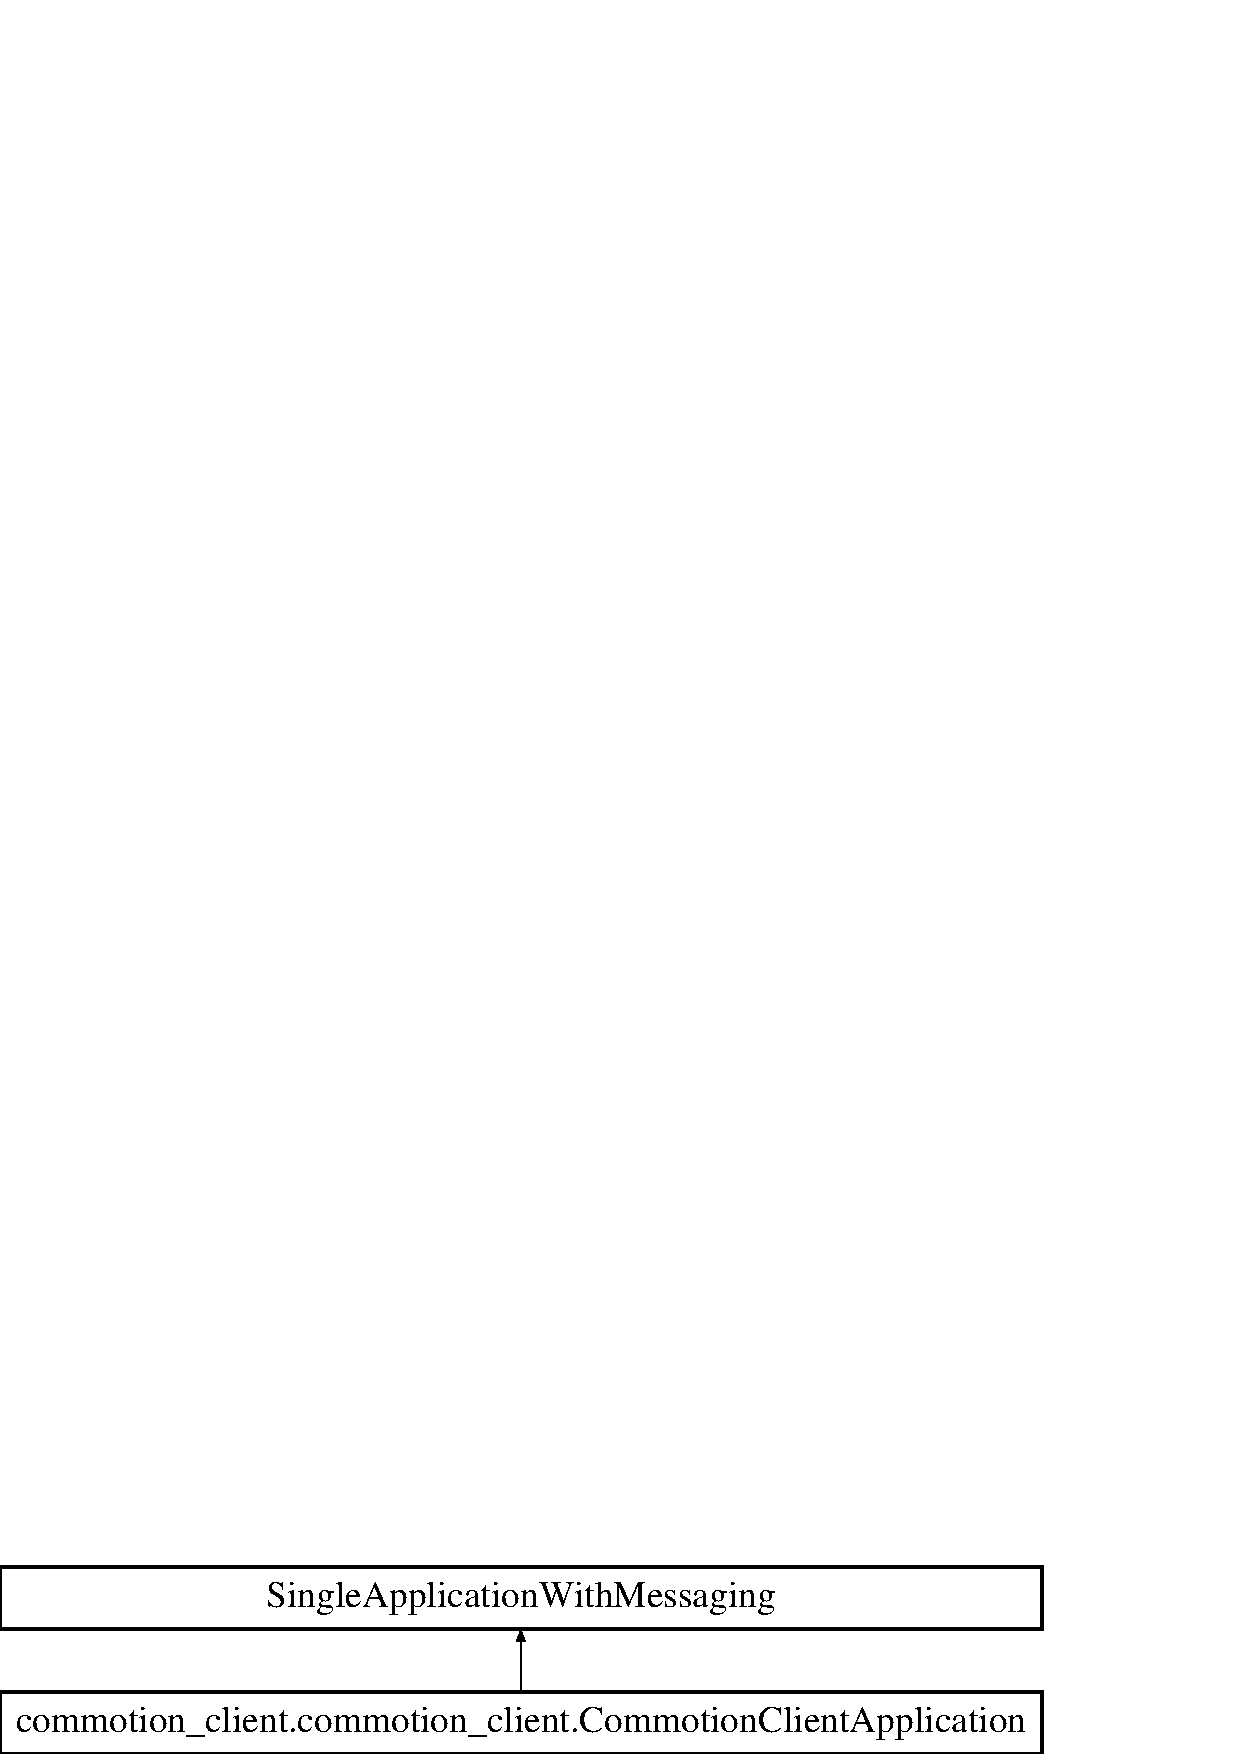
\includegraphics[height=2.000000cm]{classcommotion__client_1_1commotion__client_1_1CommotionClientApplication}
\end{center}
\end{figure}
\subsection*{Public Member Functions}
\begin{DoxyCompactItemize}
\item 
\hypertarget{classcommotion__client_1_1commotion__client_1_1CommotionClientApplication_af131eabc9f0007d5d8541228988767ca}{def {\bfseries \+\_\+\+\_\+init\+\_\+\+\_\+}}\label{classcommotion__client_1_1commotion__client_1_1CommotionClientApplication_af131eabc9f0007d5d8541228988767ca}

\item 
def \hyperlink{classcommotion__client_1_1commotion__client_1_1CommotionClientApplication_adbf0b01d9e64047a4ad7971161d457b1}{init\+\_\+client}
\item 
\hypertarget{classcommotion__client_1_1commotion__client_1_1CommotionClientApplication_aecf3bce1170d5ec27871002233b8a389}{def {\bfseries init\+\_\+logging}}\label{classcommotion__client_1_1commotion__client_1_1CommotionClientApplication_aecf3bce1170d5ec27871002233b8a389}

\item 
def \hyperlink{classcommotion__client_1_1commotion__client_1_1CommotionClientApplication_a61c21aa424a10a251b3a2902b3740bbe}{start\+\_\+full}
\item 
def \hyperlink{classcommotion__client_1_1commotion__client_1_1CommotionClientApplication_a640d7d7d8306a2e6ee7b66fa8281f5f5}{start\+\_\+daemon}
\item 
def \hyperlink{classcommotion__client_1_1commotion__client_1_1CommotionClientApplication_a63104a06ba20d9b679c22b542fd90c94}{stop\+\_\+client}
\item 
def \hyperlink{classcommotion__client_1_1commotion__client_1_1CommotionClientApplication_af40aa0ed2df54b7edb7f3e474b336a63}{restart\+\_\+client}
\item 
def \hyperlink{classcommotion__client_1_1commotion__client_1_1CommotionClientApplication_a726949d610a2bd566d1f3745b74c7b42}{create\+\_\+main\+\_\+window}
\item 
def \hyperlink{classcommotion__client_1_1commotion__client_1_1CommotionClientApplication_a1ed67f317a1ddd84b65ef39a848732bf}{init\+\_\+main}
\item 
def \hyperlink{classcommotion__client_1_1commotion__client_1_1CommotionClientApplication_a6b8f22fc6aaab6e6105f7832a7bf11b9}{hide\+\_\+main\+\_\+window}
\item 
def \hyperlink{classcommotion__client_1_1commotion__client_1_1CommotionClientApplication_ac3f5efd893879314eb1fbcf7e4d90192}{close\+\_\+main\+\_\+window}
\item 
def \hyperlink{classcommotion__client_1_1commotion__client_1_1CommotionClientApplication_a6afd07f83f02108c04a682120bd5a298}{create\+\_\+controller}
\item 
\hypertarget{classcommotion__client_1_1commotion__client_1_1CommotionClientApplication_ac6c092a34ad6d9174135769da24671f5}{def {\bfseries init\+\_\+controller}}\label{classcommotion__client_1_1commotion__client_1_1CommotionClientApplication_ac6c092a34ad6d9174135769da24671f5}

\item 
def \hyperlink{classcommotion__client_1_1commotion__client_1_1CommotionClientApplication_aa35cc13c36cfa90d6ac3de6db56e5fc4}{close\+\_\+controller}
\item 
def \hyperlink{classcommotion__client_1_1commotion__client_1_1CommotionClientApplication_a12d73b88d1b926747be8b29fc38b584b}{init\+\_\+sys\+\_\+tray}
\item 
def \hyperlink{classcommotion__client_1_1commotion__client_1_1CommotionClientApplication_a8925f9e653516a05ab38377a05442ac2}{create\+\_\+sys\+\_\+tray}
\item 
def \hyperlink{classcommotion__client_1_1commotion__client_1_1CommotionClientApplication_a2a0f0cfc9ca6a62a2aaa90bdc8bca1fc}{close\+\_\+sys\+\_\+tray}
\item 
def \hyperlink{classcommotion__client_1_1commotion__client_1_1CommotionClientApplication_a981d54a4d40a4345a253be2b2a541127}{process\+\_\+message}
\item 
def \hyperlink{classcommotion__client_1_1commotion__client_1_1CommotionClientApplication_af2043aac2ebc25f55b73ec317d6ea463}{end}
\end{DoxyCompactItemize}
\subsection*{Public Attributes}
\begin{DoxyCompactItemize}
\item 
\hypertarget{classcommotion__client_1_1commotion__client_1_1CommotionClientApplication_a57e951c9b241fb0e0c70055b4ca1b6f7}{{\bfseries translate}}\label{classcommotion__client_1_1commotion__client_1_1CommotionClientApplication_a57e951c9b241fb0e0c70055b4ca1b6f7}

\item 
\hypertarget{classcommotion__client_1_1commotion__client_1_1CommotionClientApplication_ac61adc90b20e338b91b2b3fe9032d3e3}{{\bfseries status}}\label{classcommotion__client_1_1commotion__client_1_1CommotionClientApplication_ac61adc90b20e338b91b2b3fe9032d3e3}

\item 
\hypertarget{classcommotion__client_1_1commotion__client_1_1CommotionClientApplication_a2def597b4431ad9a5dbb7ce4339ba0e0}{{\bfseries controller}}\label{classcommotion__client_1_1commotion__client_1_1CommotionClientApplication_a2def597b4431ad9a5dbb7ce4339ba0e0}

\item 
\hypertarget{classcommotion__client_1_1commotion__client_1_1CommotionClientApplication_a4ae692cf60dc0a935cf2e8a72f657d1a}{{\bfseries main}}\label{classcommotion__client_1_1commotion__client_1_1CommotionClientApplication_a4ae692cf60dc0a935cf2e8a72f657d1a}

\item 
\hypertarget{classcommotion__client_1_1commotion__client_1_1CommotionClientApplication_a48a8bf39339f834c94353ca68444176f}{{\bfseries sys\+\_\+tray}}\label{classcommotion__client_1_1commotion__client_1_1CommotionClientApplication_a48a8bf39339f834c94353ca68444176f}

\item 
\hypertarget{classcommotion__client_1_1commotion__client_1_1CommotionClientApplication_a4d1d6381f0c2e68362f6f83eb4fd13c0}{{\bfseries logger}}\label{classcommotion__client_1_1commotion__client_1_1CommotionClientApplication_a4d1d6381f0c2e68362f6f83eb4fd13c0}

\item 
\hypertarget{classcommotion__client_1_1commotion__client_1_1CommotionClientApplication_a1435afc4782f96f59c68845e98a1164e}{{\bfseries log}}\label{classcommotion__client_1_1commotion__client_1_1CommotionClientApplication_a1435afc4782f96f59c68845e98a1164e}

\end{DoxyCompactItemize}
\subsection*{Static Public Attributes}
\begin{DoxyCompactItemize}
\item 
\hypertarget{classcommotion__client_1_1commotion__client_1_1CommotionClientApplication_af808e792c256914e6af9813b48bb8f83}{tuple {\bfseries restarted} = Qt\+Core.\+pyqt\+Signal()}\label{classcommotion__client_1_1commotion__client_1_1CommotionClientApplication_af808e792c256914e6af9813b48bb8f83}

\end{DoxyCompactItemize}


\subsection{Detailed Description}
\begin{DoxyVerb}The final layer of the class onion that is the Commotion client. This class includes functions to enable the sub-processes and modules of the Commotion Client (GUI's and controllers). 
\end{DoxyVerb}
 

\subsection{Member Function Documentation}
\hypertarget{classcommotion__client_1_1commotion__client_1_1CommotionClientApplication_aa35cc13c36cfa90d6ac3de6db56e5fc4}{\index{commotion\+\_\+client\+::commotion\+\_\+client\+::\+Commotion\+Client\+Application@{commotion\+\_\+client\+::commotion\+\_\+client\+::\+Commotion\+Client\+Application}!close\+\_\+controller@{close\+\_\+controller}}
\index{close\+\_\+controller@{close\+\_\+controller}!commotion\+\_\+client\+::commotion\+\_\+client\+::\+Commotion\+Client\+Application@{commotion\+\_\+client\+::commotion\+\_\+client\+::\+Commotion\+Client\+Application}}
\subsubsection[{close\+\_\+controller}]{\setlength{\rightskip}{0pt plus 5cm}def commotion\+\_\+client.\+commotion\+\_\+client.\+Commotion\+Client\+Application.\+close\+\_\+controller (
\begin{DoxyParamCaption}
\item[{}]{self, }
\item[{}]{force\+\_\+close = {\ttfamily None}}
\end{DoxyParamCaption}
)}}\label{classcommotion__client_1_1commotion__client_1_1CommotionClientApplication_aa35cc13c36cfa90d6ac3de6db56e5fc4}
\begin{DoxyVerb}Closes the controller process.

@param force_close bool If the application fails to kill the controller, the whole application should be shut down.
\end{DoxyVerb}
 

Referenced by commotion\+\_\+client.\+commotion\+\_\+client.\+Commotion\+Client\+Application.\+stop\+\_\+client().


\begin{DoxyCode}
403 
404     \textcolor{keyword}{def }\hyperlink{classcommotion__client_1_1commotion__client_1_1CommotionClientApplication_aa35cc13c36cfa90d6ac3de6db56e5fc4}{close\_controller}(self, force\_close=None):
405         \textcolor{stringliteral}{"""}
406 \textcolor{stringliteral}{        Closes the controller process.}
407 \textcolor{stringliteral}{}
408 \textcolor{stringliteral}{        @param force\_close bool If the application fails to kill the controller, the whole application
       should be shut down.}
409 \textcolor{stringliteral}{        """}
410         \textcolor{keywordflow}{try}:
411             \textcolor{keywordflow}{pass} \textcolor{comment}{#TODO Swap with below when controller close function is instantiated}
412             \textcolor{comment}{#if self.controller.close():}
413             \textcolor{comment}{#    self.controller = None}
414         \textcolor{keywordflow}{except} Exception \textcolor{keyword}{as} \_excp:
415             self.log.error(self.\hyperlink{classcommotion__client_1_1commotion__client_1_1CommotionClientApplication_a57e951c9b241fb0e0c70055b4ca1b6f7}{translate}(\textcolor{stringliteral}{"logs"}, \textcolor{stringliteral}{"Could not close controller."}))
416             \textcolor{keywordflow}{if} force\_close:
417                 self.log.info(self.\hyperlink{classcommotion__client_1_1commotion__client_1_1CommotionClientApplication_a57e951c9b241fb0e0c70055b4ca1b6f7}{translate}(\textcolor{stringliteral}{"logs"}, \textcolor{stringliteral}{"force\_close activated. Closing application."}
      ))
418                 \textcolor{keywordflow}{try}:
419                     del self.\hyperlink{classcommotion__client_1_1commotion__client_1_1CommotionClientApplication_a2def597b4431ad9a5dbb7ce4339ba0e0}{controller}
420                 \textcolor{keywordflow}{except} Exception \textcolor{keyword}{as} \_excp:
421                     \_catch\_all = self.\hyperlink{classcommotion__client_1_1commotion__client_1_1CommotionClientApplication_a57e951c9b241fb0e0c70055b4ca1b6f7}{translate}(\textcolor{stringliteral}{"logs"}, \textcolor{stringliteral}{"Could not close controller using its
       internal mechanisms. Application will be halted."})
422                     self.log.critical(\_catch\_all)
423                     self.log.exception(\_excp)
424                     self.\hyperlink{classcommotion__client_1_1commotion__client_1_1CommotionClientApplication_af2043aac2ebc25f55b73ec317d6ea463}{end}(\_catch\_all)
425             \textcolor{keywordflow}{else}:
426                 self.log.error(self.\hyperlink{classcommotion__client_1_1commotion__client_1_1CommotionClientApplication_a57e951c9b241fb0e0c70055b4ca1b6f7}{translate}(\textcolor{stringliteral}{"logs"}, \textcolor{stringliteral}{"Could not cleanly close controller."}))
427                 self.log.info(self.\hyperlink{classcommotion__client_1_1commotion__client_1_1CommotionClientApplication_a57e951c9b241fb0e0c70055b4ca1b6f7}{translate}(\textcolor{stringliteral}{"logs"}, \textcolor{stringliteral}{"It is reccomended that you close the entire
       application."}))
428                 self.log.exception(\_excp)
429                 \textcolor{keywordflow}{raise}
430 
431 
432 \textcolor{comment}{#=================================================}
433 \textcolor{comment}{#                 SYSTEM TRAY}
434 \textcolor{comment}{#=================================================}
            
\end{DoxyCode}
\hypertarget{classcommotion__client_1_1commotion__client_1_1CommotionClientApplication_ac3f5efd893879314eb1fbcf7e4d90192}{\index{commotion\+\_\+client\+::commotion\+\_\+client\+::\+Commotion\+Client\+Application@{commotion\+\_\+client\+::commotion\+\_\+client\+::\+Commotion\+Client\+Application}!close\+\_\+main\+\_\+window@{close\+\_\+main\+\_\+window}}
\index{close\+\_\+main\+\_\+window@{close\+\_\+main\+\_\+window}!commotion\+\_\+client\+::commotion\+\_\+client\+::\+Commotion\+Client\+Application@{commotion\+\_\+client\+::commotion\+\_\+client\+::\+Commotion\+Client\+Application}}
\subsubsection[{close\+\_\+main\+\_\+window}]{\setlength{\rightskip}{0pt plus 5cm}def commotion\+\_\+client.\+commotion\+\_\+client.\+Commotion\+Client\+Application.\+close\+\_\+main\+\_\+window (
\begin{DoxyParamCaption}
\item[{}]{self, }
\item[{}]{force\+\_\+close = {\ttfamily None}}
\end{DoxyParamCaption}
)}}\label{classcommotion__client_1_1commotion__client_1_1CommotionClientApplication_ac3f5efd893879314eb1fbcf7e4d90192}
\begin{DoxyVerb}Closes the main window and task-bar. Only removes the GUI components without closing the application.

@param force_close bool If the application fails to kill the main window, the whole application should be shut down.
@return bool
\end{DoxyVerb}
 

References commotion\+\_\+client.\+commotion\+\_\+client.\+Hold\+State\+During\+Restart.\+end(), commotion\+\_\+client.\+commotion\+\_\+client.\+Commotion\+Client\+Application.\+end(), commotion\+\_\+client.\+commotion\+\_\+client.\+Commotion\+Client\+Application.\+main, and commotion\+\_\+client.\+commotion\+\_\+client.\+Commotion\+Client\+Application.\+translate.



Referenced by commotion\+\_\+client.\+commotion\+\_\+client.\+Commotion\+Client\+Application.\+hide\+\_\+main\+\_\+window(), and commotion\+\_\+client.\+commotion\+\_\+client.\+Commotion\+Client\+Application.\+stop\+\_\+client().


\begin{DoxyCode}
355 
356     \textcolor{keyword}{def }\hyperlink{classcommotion__client_1_1commotion__client_1_1CommotionClientApplication_ac3f5efd893879314eb1fbcf7e4d90192}{close\_main\_window}(self, force\_close=None):
357         \textcolor{stringliteral}{"""}
358 \textcolor{stringliteral}{        Closes the main window and task-bar. Only removes the GUI components without closing the
       application.}
359 \textcolor{stringliteral}{}
360 \textcolor{stringliteral}{        @param force\_close bool If the application fails to kill the main window, the whole application
       should be shut down.}
361 \textcolor{stringliteral}{        @return bool}
362 \textcolor{stringliteral}{        """}
363         \textcolor{keywordflow}{try}:
364             self.main.purge
365             self.\hyperlink{classcommotion__client_1_1commotion__client_1_1CommotionClientApplication_a4ae692cf60dc0a935cf2e8a72f657d1a}{main} = \textcolor{keyword}{False}
366         \textcolor{keywordflow}{except} Exception \textcolor{keyword}{as} \_excp:
367             self.log.error(self.\hyperlink{classcommotion__client_1_1commotion__client_1_1CommotionClientApplication_a57e951c9b241fb0e0c70055b4ca1b6f7}{translate}(\textcolor{stringliteral}{"logs"}, \textcolor{stringliteral}{"Could not close main window."}))
368             \textcolor{keywordflow}{if} force\_close:
369                 self.log.info(self.\hyperlink{classcommotion__client_1_1commotion__client_1_1CommotionClientApplication_a57e951c9b241fb0e0c70055b4ca1b6f7}{translate}(\textcolor{stringliteral}{"logs"}, \textcolor{stringliteral}{"force\_close activated. Closing application."}
      ))
370                 \textcolor{keywordflow}{try}:
371                     self.main.deleteLater()
372                     self.\hyperlink{classcommotion__client_1_1commotion__client_1_1CommotionClientApplication_a4ae692cf60dc0a935cf2e8a72f657d1a}{main} = \textcolor{keyword}{False}
373                 \textcolor{keywordflow}{except} Exception \textcolor{keyword}{as} \_excp:
374                     \_catch\_all = self.\hyperlink{classcommotion__client_1_1commotion__client_1_1CommotionClientApplication_a57e951c9b241fb0e0c70055b4ca1b6f7}{translate}(\textcolor{stringliteral}{"logs"}, \textcolor{stringliteral}{"Could not close main window using its
       internal mechanisms. Application will be halted."})
375                     self.log.critical(\_catch\_all)
376                     self.log.exception(\_excp)
377                     self.\hyperlink{classcommotion__client_1_1commotion__client_1_1CommotionClientApplication_af2043aac2ebc25f55b73ec317d6ea463}{end}(\_catch\_all)
378             \textcolor{keywordflow}{else}:
379                 self.log.error(self.\hyperlink{classcommotion__client_1_1commotion__client_1_1CommotionClientApplication_a57e951c9b241fb0e0c70055b4ca1b6f7}{translate}(\textcolor{stringliteral}{"logs"}, \textcolor{stringliteral}{"Could not close main window."}))
380                 self.log.info(self.\hyperlink{classcommotion__client_1_1commotion__client_1_1CommotionClientApplication_a57e951c9b241fb0e0c70055b4ca1b6f7}{translate}(\textcolor{stringliteral}{"logs"}, \textcolor{stringliteral}{"It is reccomended that you close the entire
       application."}))
381                 self.log.exception(\_excp)
382                 \textcolor{keywordflow}{raise}
383 
384 \textcolor{comment}{#=================================================}
385 \textcolor{comment}{#                 CONTROLLER}
386 \textcolor{comment}{#=================================================}

\end{DoxyCode}
\hypertarget{classcommotion__client_1_1commotion__client_1_1CommotionClientApplication_a2a0f0cfc9ca6a62a2aaa90bdc8bca1fc}{\index{commotion\+\_\+client\+::commotion\+\_\+client\+::\+Commotion\+Client\+Application@{commotion\+\_\+client\+::commotion\+\_\+client\+::\+Commotion\+Client\+Application}!close\+\_\+sys\+\_\+tray@{close\+\_\+sys\+\_\+tray}}
\index{close\+\_\+sys\+\_\+tray@{close\+\_\+sys\+\_\+tray}!commotion\+\_\+client\+::commotion\+\_\+client\+::\+Commotion\+Client\+Application@{commotion\+\_\+client\+::commotion\+\_\+client\+::\+Commotion\+Client\+Application}}
\subsubsection[{close\+\_\+sys\+\_\+tray}]{\setlength{\rightskip}{0pt plus 5cm}def commotion\+\_\+client.\+commotion\+\_\+client.\+Commotion\+Client\+Application.\+close\+\_\+sys\+\_\+tray (
\begin{DoxyParamCaption}
\item[{}]{self, }
\item[{}]{force\+\_\+close = {\ttfamily None}}
\end{DoxyParamCaption}
)}}\label{classcommotion__client_1_1commotion__client_1_1CommotionClientApplication_a2a0f0cfc9ca6a62a2aaa90bdc8bca1fc}
\begin{DoxyVerb}Closes the system tray. Only removes the GUI components without closing the application.

@param force_close bool If the application fails to kill the main window, the whole application should be shut down.
@return bool 
\end{DoxyVerb}
 

References commotion\+\_\+client.\+commotion\+\_\+client.\+Hold\+State\+During\+Restart.\+end(), commotion\+\_\+client.\+commotion\+\_\+client.\+Commotion\+Client\+Application.\+end(), commotion\+\_\+client.\+commotion\+\_\+client.\+Commotion\+Client\+Application.\+sys\+\_\+tray, and commotion\+\_\+client.\+commotion\+\_\+client.\+Commotion\+Client\+Application.\+translate.



Referenced by commotion\+\_\+client.\+commotion\+\_\+client.\+Commotion\+Client\+Application.\+stop\+\_\+client().


\begin{DoxyCode}
461 
462     \textcolor{keyword}{def }\hyperlink{classcommotion__client_1_1commotion__client_1_1CommotionClientApplication_a2a0f0cfc9ca6a62a2aaa90bdc8bca1fc}{close\_sys\_tray}(self, force\_close=None):
463         \textcolor{stringliteral}{"""}
464 \textcolor{stringliteral}{        Closes the system tray. Only removes the GUI components without closing the application.}
465 \textcolor{stringliteral}{}
466 \textcolor{stringliteral}{        @param force\_close bool If the application fails to kill the main window, the whole application
       should be shut down.}
467 \textcolor{stringliteral}{        @return bool }
468 \textcolor{stringliteral}{        """}
469         \textcolor{keywordflow}{try}:
470             self.sys\_tray.close()
471             self.\hyperlink{classcommotion__client_1_1commotion__client_1_1CommotionClientApplication_a48a8bf39339f834c94353ca68444176f}{sys\_tray} = \textcolor{keyword}{False}
472         \textcolor{keywordflow}{except} Exception \textcolor{keyword}{as} \_excp:
473             self.log.error(self.\hyperlink{classcommotion__client_1_1commotion__client_1_1CommotionClientApplication_a57e951c9b241fb0e0c70055b4ca1b6f7}{translate}(\textcolor{stringliteral}{"logs"}, \textcolor{stringliteral}{"Could not close system tray."}))
474             \textcolor{keywordflow}{if} force\_close:
475                 self.log.info(self.\hyperlink{classcommotion__client_1_1commotion__client_1_1CommotionClientApplication_a57e951c9b241fb0e0c70055b4ca1b6f7}{translate}(\textcolor{stringliteral}{"logs"}, \textcolor{stringliteral}{"force\_close activated. Closing application."}
      ))
476                 \textcolor{keywordflow}{try}:
477                     self.sys\_tray.deleteLater()
478                     self.sys\_tray.close()
479                 \textcolor{keywordflow}{except}:
480                     \_catch\_all = self.\hyperlink{classcommotion__client_1_1commotion__client_1_1CommotionClientApplication_a57e951c9b241fb0e0c70055b4ca1b6f7}{translate}(\textcolor{stringliteral}{"logs"}, \textcolor{stringliteral}{"Could not close system tray using its
       internal mechanisms. Application will be halted."})
481                     self.log.critical(\_catch\_all)
482                     self.log.exception(\_excp)
483                     self.\hyperlink{classcommotion__client_1_1commotion__client_1_1CommotionClientApplication_af2043aac2ebc25f55b73ec317d6ea463}{end}(\_catch\_all)
484             \textcolor{keywordflow}{else}:
485                 self.log.error(self.\hyperlink{classcommotion__client_1_1commotion__client_1_1CommotionClientApplication_a57e951c9b241fb0e0c70055b4ca1b6f7}{translate}(\textcolor{stringliteral}{"logs"}, \textcolor{stringliteral}{"Could not close system tray."}))
486                 self.log.info(self.\hyperlink{classcommotion__client_1_1commotion__client_1_1CommotionClientApplication_a57e951c9b241fb0e0c70055b4ca1b6f7}{translate}(\textcolor{stringliteral}{"logs"}, \textcolor{stringliteral}{"It is reccomended that you close the entire
       application."}))
487                 self.log.exception(\_excp)
488                 \textcolor{keywordflow}{raise}
489 
490 \textcolor{comment}{#=================================================}
491 \textcolor{comment}{#               APPLICATION UTILS}
492 \textcolor{comment}{#=================================================}

\end{DoxyCode}
\hypertarget{classcommotion__client_1_1commotion__client_1_1CommotionClientApplication_a6afd07f83f02108c04a682120bd5a298}{\index{commotion\+\_\+client\+::commotion\+\_\+client\+::\+Commotion\+Client\+Application@{commotion\+\_\+client\+::commotion\+\_\+client\+::\+Commotion\+Client\+Application}!create\+\_\+controller@{create\+\_\+controller}}
\index{create\+\_\+controller@{create\+\_\+controller}!commotion\+\_\+client\+::commotion\+\_\+client\+::\+Commotion\+Client\+Application@{commotion\+\_\+client\+::commotion\+\_\+client\+::\+Commotion\+Client\+Application}}
\subsubsection[{create\+\_\+controller}]{\setlength{\rightskip}{0pt plus 5cm}def commotion\+\_\+client.\+commotion\+\_\+client.\+Commotion\+Client\+Application.\+create\+\_\+controller (
\begin{DoxyParamCaption}
\item[{}]{self}
\end{DoxyParamCaption}
)}}\label{classcommotion__client_1_1commotion__client_1_1CommotionClientApplication_a6afd07f83f02108c04a682120bd5a298}
\begin{DoxyVerb}Creates a controller to act as the middleware between the GUI and the commotion core.
\end{DoxyVerb}
 

References commotion\+\_\+client.\+commotion\+\_\+client.\+Commotion\+Client\+Application.\+translate.


\begin{DoxyCode}
387 
388     \textcolor{keyword}{def }\hyperlink{classcommotion__client_1_1commotion__client_1_1CommotionClientApplication_a6afd07f83f02108c04a682120bd5a298}{create\_controller}(self):
389         \textcolor{stringliteral}{"""}
390 \textcolor{stringliteral}{        Creates a controller to act as the middleware between the GUI and the commotion core.}
391 \textcolor{stringliteral}{        """}
392         \textcolor{keywordflow}{try}:
393             \textcolor{keywordflow}{pass} \textcolor{comment}{#replace when controller is ready}
394             \textcolor{comment}{#self.controller = CommotionController() #TODO Implement controller}
395             \textcolor{comment}{#self.controller.init() #??????}
396         \textcolor{keywordflow}{except} Exception \textcolor{keyword}{as} \_excp:
397             self.log.critical(self.\hyperlink{classcommotion__client_1_1commotion__client_1_1CommotionClientApplication_a57e951c9b241fb0e0c70055b4ca1b6f7}{translate}(\textcolor{stringliteral}{"logs"}, \textcolor{stringliteral}{"Could not create controller. Application
       must be halted."}))
398             self.log.exception(\_excp)
399             \textcolor{keywordflow}{raise}

\end{DoxyCode}
\hypertarget{classcommotion__client_1_1commotion__client_1_1CommotionClientApplication_a726949d610a2bd566d1f3745b74c7b42}{\index{commotion\+\_\+client\+::commotion\+\_\+client\+::\+Commotion\+Client\+Application@{commotion\+\_\+client\+::commotion\+\_\+client\+::\+Commotion\+Client\+Application}!create\+\_\+main\+\_\+window@{create\+\_\+main\+\_\+window}}
\index{create\+\_\+main\+\_\+window@{create\+\_\+main\+\_\+window}!commotion\+\_\+client\+::commotion\+\_\+client\+::\+Commotion\+Client\+Application@{commotion\+\_\+client\+::commotion\+\_\+client\+::\+Commotion\+Client\+Application}}
\subsubsection[{create\+\_\+main\+\_\+window}]{\setlength{\rightskip}{0pt plus 5cm}def commotion\+\_\+client.\+commotion\+\_\+client.\+Commotion\+Client\+Application.\+create\+\_\+main\+\_\+window (
\begin{DoxyParamCaption}
\item[{}]{self}
\end{DoxyParamCaption}
)}}\label{classcommotion__client_1_1commotion__client_1_1CommotionClientApplication_a726949d610a2bd566d1f3745b74c7b42}
\begin{DoxyVerb}Will create a new main window or return existing main window if one is already created.
\end{DoxyVerb}
 

References commotion\+\_\+client.\+commotion\+\_\+client.\+Commotion\+Client\+Application.\+main, and commotion\+\_\+client.\+commotion\+\_\+client.\+Commotion\+Client\+Application.\+translate.



Referenced by commotion\+\_\+client.\+commotion\+\_\+client.\+Commotion\+Client\+Application.\+hide\+\_\+main\+\_\+window(), and commotion\+\_\+client.\+commotion\+\_\+client.\+Commotion\+Client\+Application.\+start\+\_\+full().


\begin{DoxyCode}
272 
273     \textcolor{keyword}{def }\hyperlink{classcommotion__client_1_1commotion__client_1_1CommotionClientApplication_a726949d610a2bd566d1f3745b74c7b42}{create\_main\_window}(self):
274         \textcolor{stringliteral}{"""}
275 \textcolor{stringliteral}{        Will create a new main window or return existing main window if one is already created.}
276 \textcolor{stringliteral}{        """}
277         \textcolor{keywordflow}{if} self.\hyperlink{classcommotion__client_1_1commotion__client_1_1CommotionClientApplication_a4ae692cf60dc0a935cf2e8a72f657d1a}{main}:
278             self.log.debug(self.\hyperlink{classcommotion__client_1_1commotion__client_1_1CommotionClientApplication_a57e951c9b241fb0e0c70055b4ca1b6f7}{translate}(\textcolor{stringliteral}{"logs"}, \textcolor{stringliteral}{"New window requested when one already exists.
       Returning existing main window."}))
279             self.log.info(self.\hyperlink{classcommotion__client_1_1commotion__client_1_1CommotionClientApplication_a57e951c9b241fb0e0c70055b4ca1b6f7}{translate}(\textcolor{stringliteral}{"logs"}, \textcolor{stringliteral}{"If you would like to close the main window and
       re-open it please call close\_main\_window() first."}))
280             \textcolor{keywordflow}{return} self.\hyperlink{classcommotion__client_1_1commotion__client_1_1CommotionClientApplication_a4ae692cf60dc0a935cf2e8a72f657d1a}{main}
281         \textcolor{keywordflow}{try}:
282             \_main = main\_window.MainWindow()
283         \textcolor{keywordflow}{except} Exception \textcolor{keyword}{as} \_excp:
284             self.log.critical(self.\hyperlink{classcommotion__client_1_1commotion__client_1_1CommotionClientApplication_a57e951c9b241fb0e0c70055b4ca1b6f7}{translate}(\textcolor{stringliteral}{"logs"}, \textcolor{stringliteral}{"Could not create Main Window. Application
       must be halted."}))
285             \textcolor{keywordflow}{raise}
286         \textcolor{keywordflow}{else}:
287             \textcolor{keywordflow}{return} \_main

\end{DoxyCode}
\hypertarget{classcommotion__client_1_1commotion__client_1_1CommotionClientApplication_a8925f9e653516a05ab38377a05442ac2}{\index{commotion\+\_\+client\+::commotion\+\_\+client\+::\+Commotion\+Client\+Application@{commotion\+\_\+client\+::commotion\+\_\+client\+::\+Commotion\+Client\+Application}!create\+\_\+sys\+\_\+tray@{create\+\_\+sys\+\_\+tray}}
\index{create\+\_\+sys\+\_\+tray@{create\+\_\+sys\+\_\+tray}!commotion\+\_\+client\+::commotion\+\_\+client\+::\+Commotion\+Client\+Application@{commotion\+\_\+client\+::commotion\+\_\+client\+::\+Commotion\+Client\+Application}}
\subsubsection[{create\+\_\+sys\+\_\+tray}]{\setlength{\rightskip}{0pt plus 5cm}def commotion\+\_\+client.\+commotion\+\_\+client.\+Commotion\+Client\+Application.\+create\+\_\+sys\+\_\+tray (
\begin{DoxyParamCaption}
\item[{}]{self}
\end{DoxyParamCaption}
)}}\label{classcommotion__client_1_1commotion__client_1_1CommotionClientApplication_a8925f9e653516a05ab38377a05442ac2}
\begin{DoxyVerb}Starts the system tray
\end{DoxyVerb}
 

References commotion\+\_\+client.\+commotion\+\_\+client.\+Commotion\+Client\+Application.\+translate.



Referenced by commotion\+\_\+client.\+commotion\+\_\+client.\+Commotion\+Client\+Application.\+start\+\_\+daemon(), and commotion\+\_\+client.\+commotion\+\_\+client.\+Commotion\+Client\+Application.\+start\+\_\+full().


\begin{DoxyCode}
448 
449     \textcolor{keyword}{def }\hyperlink{classcommotion__client_1_1commotion__client_1_1CommotionClientApplication_a8925f9e653516a05ab38377a05442ac2}{create\_sys\_tray}(self):
450         \textcolor{stringliteral}{"""}
451 \textcolor{stringliteral}{        Starts the system tray}
452 \textcolor{stringliteral}{        """}
453         \textcolor{keywordflow}{try}:
454             tray = system\_tray.TrayIcon()
455         \textcolor{keywordflow}{except} Exception \textcolor{keyword}{as} \_excp:
456             self.log.error(self.\hyperlink{classcommotion__client_1_1commotion__client_1_1CommotionClientApplication_a57e951c9b241fb0e0c70055b4ca1b6f7}{translate}(\textcolor{stringliteral}{"logs"}, \textcolor{stringliteral}{"Could not start system tray."}))
457             self.log.exception(\_excp)
458             \textcolor{keywordflow}{raise}
459         \textcolor{keywordflow}{else}:
460             \textcolor{keywordflow}{return} tray

\end{DoxyCode}
\hypertarget{classcommotion__client_1_1commotion__client_1_1CommotionClientApplication_af2043aac2ebc25f55b73ec317d6ea463}{\index{commotion\+\_\+client\+::commotion\+\_\+client\+::\+Commotion\+Client\+Application@{commotion\+\_\+client\+::commotion\+\_\+client\+::\+Commotion\+Client\+Application}!end@{end}}
\index{end@{end}!commotion\+\_\+client\+::commotion\+\_\+client\+::\+Commotion\+Client\+Application@{commotion\+\_\+client\+::commotion\+\_\+client\+::\+Commotion\+Client\+Application}}
\subsubsection[{end}]{\setlength{\rightskip}{0pt plus 5cm}def commotion\+\_\+client.\+commotion\+\_\+client.\+Commotion\+Client\+Application.\+end (
\begin{DoxyParamCaption}
\item[{}]{self, }
\item[{}]{message = {\ttfamily None}}
\end{DoxyParamCaption}
)}}\label{classcommotion__client_1_1commotion__client_1_1CommotionClientApplication_af2043aac2ebc25f55b73ec317d6ea463}
\begin{DoxyVerb}Handles properly exiting the application.

@param message string optional exit message to print to standard error on application close. This will FORCE the application to close in an unclean way.
\end{DoxyVerb}
 

References commotion\+\_\+client.\+G\+U\+I.\+system\+\_\+tray.\+Tray\+Icon.\+exit, and commotion\+\_\+client.\+commotion\+\_\+client.\+Commotion\+Client\+Application.\+translate.



Referenced by commotion\+\_\+client.\+commotion\+\_\+client.\+Commotion\+Client\+Application.\+close\+\_\+controller(), commotion\+\_\+client.\+commotion\+\_\+client.\+Commotion\+Client\+Application.\+close\+\_\+main\+\_\+window(), commotion\+\_\+client.\+commotion\+\_\+client.\+Commotion\+Client\+Application.\+close\+\_\+sys\+\_\+tray(), commotion\+\_\+client.\+commotion\+\_\+client.\+Commotion\+Client\+Application.\+init\+\_\+client(), commotion\+\_\+client.\+commotion\+\_\+client.\+Commotion\+Client\+Application.\+restart\+\_\+client(), commotion\+\_\+client.\+commotion\+\_\+client.\+Commotion\+Client\+Application.\+start\+\_\+full(), and commotion\+\_\+client.\+commotion\+\_\+client.\+Commotion\+Client\+Application.\+stop\+\_\+client().


\begin{DoxyCode}
509 
510     \textcolor{keyword}{def }\hyperlink{classcommotion__client_1_1commotion__client_1_1CommotionClientApplication_af2043aac2ebc25f55b73ec317d6ea463}{end}(self, message=None):
511         \textcolor{stringliteral}{"""}
512 \textcolor{stringliteral}{        Handles properly exiting the application.}
513 \textcolor{stringliteral}{}
514 \textcolor{stringliteral}{        @param message string optional exit message to print to standard error on application close. This
       will FORCE the application to close in an unclean way.}
515 \textcolor{stringliteral}{        """}
516         \textcolor{keywordflow}{if} message:
517             self.log.error(self.\hyperlink{classcommotion__client_1_1commotion__client_1_1CommotionClientApplication_a57e951c9b241fb0e0c70055b4ca1b6f7}{translate}(\textcolor{stringliteral}{"logs"}, message))
518             self.exit(1)
519         \textcolor{keywordflow}{else}:
520             self.quit()

\end{DoxyCode}
\hypertarget{classcommotion__client_1_1commotion__client_1_1CommotionClientApplication_a6b8f22fc6aaab6e6105f7832a7bf11b9}{\index{commotion\+\_\+client\+::commotion\+\_\+client\+::\+Commotion\+Client\+Application@{commotion\+\_\+client\+::commotion\+\_\+client\+::\+Commotion\+Client\+Application}!hide\+\_\+main\+\_\+window@{hide\+\_\+main\+\_\+window}}
\index{hide\+\_\+main\+\_\+window@{hide\+\_\+main\+\_\+window}!commotion\+\_\+client\+::commotion\+\_\+client\+::\+Commotion\+Client\+Application@{commotion\+\_\+client\+::commotion\+\_\+client\+::\+Commotion\+Client\+Application}}
\subsubsection[{hide\+\_\+main\+\_\+window}]{\setlength{\rightskip}{0pt plus 5cm}def commotion\+\_\+client.\+commotion\+\_\+client.\+Commotion\+Client\+Application.\+hide\+\_\+main\+\_\+window (
\begin{DoxyParamCaption}
\item[{}]{self, }
\item[{}]{force = {\ttfamily None}, }
\item[{}]{errors = {\ttfamily None}}
\end{DoxyParamCaption}
)}}\label{classcommotion__client_1_1commotion__client_1_1CommotionClientApplication_a6b8f22fc6aaab6e6105f7832a7bf11b9}
\begin{DoxyVerb}Attempts to hide the main window without closing the task-bar.

@param force bool Force window reset if hiding is unsuccessful.
@param errors If set to "strict" errors found will be raised before returning the boolean result.
@return bool Return True if successful and false is unsuccessful.
\end{DoxyVerb}
 

References commotion\+\_\+client.\+commotion\+\_\+client.\+Commotion\+Client\+Application.\+close\+\_\+main\+\_\+window(), commotion\+\_\+client.\+commotion\+\_\+client.\+Commotion\+Client\+Application.\+create\+\_\+main\+\_\+window(), commotion\+\_\+client.\+commotion\+\_\+client.\+Commotion\+Client\+Application.\+main, commotion\+\_\+client.\+commotion\+\_\+client.\+Commotion\+Client\+Application.\+process\+\_\+message(), and commotion\+\_\+client.\+commotion\+\_\+client.\+Commotion\+Client\+Application.\+translate.



Referenced by commotion\+\_\+client.\+commotion\+\_\+client.\+Commotion\+Client\+Application.\+start\+\_\+daemon().


\begin{DoxyCode}
308 
309     \textcolor{keyword}{def }\hyperlink{classcommotion__client_1_1commotion__client_1_1CommotionClientApplication_a6b8f22fc6aaab6e6105f7832a7bf11b9}{hide\_main\_window}(self, force=None, errors=None):
310         \textcolor{stringliteral}{"""}
311 \textcolor{stringliteral}{        Attempts to hide the main window without closing the task-bar.}
312 \textcolor{stringliteral}{}
313 \textcolor{stringliteral}{        @param force bool Force window reset if hiding is unsuccessful.}
314 \textcolor{stringliteral}{        @param errors If set to "strict" errors found will be raised before returning the boolean result.}
315 \textcolor{stringliteral}{        @return bool Return True if successful and false is unsuccessful.}
316 \textcolor{stringliteral}{        """}
317         \textcolor{keywordflow}{try}:
318             self.main.exit()
319         \textcolor{keywordflow}{except} Exception \textcolor{keyword}{as} \_excp:
320             self.log.error(self.\hyperlink{classcommotion__client_1_1commotion__client_1_1CommotionClientApplication_a57e951c9b241fb0e0c70055b4ca1b6f7}{translate}(\textcolor{stringliteral}{"logs"}, \textcolor{stringliteral}{"Could not hide main window. Attempting to close
       all and only open taskbar."}))
321             self.log.exception(\_excp)
322             \textcolor{keywordflow}{if} force:
323                 \textcolor{keywordflow}{try}:
324                     self.main.purge()
325                     self.\hyperlink{classcommotion__client_1_1commotion__client_1_1CommotionClientApplication_a4ae692cf60dc0a935cf2e8a72f657d1a}{main} = \textcolor{keywordtype}{None}
326                     self.\hyperlink{classcommotion__client_1_1commotion__client_1_1CommotionClientApplication_a4ae692cf60dc0a935cf2e8a72f657d1a}{main} = self.\hyperlink{classcommotion__client_1_1commotion__client_1_1CommotionClientApplication_a726949d610a2bd566d1f3745b74c7b42}{create\_main\_window}()
327                 \textcolor{keywordflow}{except} Exception \textcolor{keyword}{as} \_excp:
328                     self.log.error(self.\hyperlink{classcommotion__client_1_1commotion__client_1_1CommotionClientApplication_a57e951c9b241fb0e0c70055b4ca1b6f7}{translate}(\textcolor{stringliteral}{"logs"}, \textcolor{stringliteral}{"Could not force main window restart."}))
329                     self.log.exception(\_excp)
330                     \textcolor{keywordflow}{raise}
331             \textcolor{keywordflow}{elif} errors == \textcolor{stringliteral}{"strict"}:
332                 \textcolor{keywordflow}{raise}
333             \textcolor{keywordflow}{else}:
334                 \textcolor{keywordflow}{return} \textcolor{keyword}{False}
335         \textcolor{keywordflow}{else}:
336             \textcolor{keywordflow}{return} \textcolor{keyword}{True}
337         \textcolor{comment}{#force hide settings}
338         \textcolor{keywordflow}{try}:
339             \textcolor{comment}{#if already open, then close first}
340             \textcolor{keywordflow}{if} self.\hyperlink{classcommotion__client_1_1commotion__client_1_1CommotionClientApplication_a4ae692cf60dc0a935cf2e8a72f657d1a}{main}:
341                 self.\hyperlink{classcommotion__client_1_1commotion__client_1_1CommotionClientApplication_ac3f5efd893879314eb1fbcf7e4d90192}{close\_main\_window}()
342             \textcolor{comment}{#re-open}
343             self.\hyperlink{classcommotion__client_1_1commotion__client_1_1CommotionClientApplication_a4ae692cf60dc0a935cf2e8a72f657d1a}{main} = main\_window.MainWindow()
344             self.main.app\_message.connect(self.\hyperlink{classcommotion__client_1_1commotion__client_1_1CommotionClientApplication_a981d54a4d40a4345a253be2b2a541127}{process\_message})
345         \textcolor{keywordflow}{except}:
346             self.log.error(self.\hyperlink{classcommotion__client_1_1commotion__client_1_1CommotionClientApplication_a57e951c9b241fb0e0c70055b4ca1b6f7}{translate}(\textcolor{stringliteral}{"logs"}, \textcolor{stringliteral}{"Could close and re-open the main window."}))
347             self.log.exception(\_excp)
348             \textcolor{keywordflow}{if} errors == \textcolor{stringliteral}{"strict"}:
349                 \textcolor{keywordflow}{raise}
350             \textcolor{keywordflow}{else}:
351                 \textcolor{keywordflow}{return} \textcolor{keyword}{False}
352         \textcolor{keywordflow}{else}:
353             \textcolor{keywordflow}{return} \textcolor{keyword}{True}
354         \textcolor{keywordflow}{return} \textcolor{keyword}{False}

\end{DoxyCode}
\hypertarget{classcommotion__client_1_1commotion__client_1_1CommotionClientApplication_adbf0b01d9e64047a4ad7971161d457b1}{\index{commotion\+\_\+client\+::commotion\+\_\+client\+::\+Commotion\+Client\+Application@{commotion\+\_\+client\+::commotion\+\_\+client\+::\+Commotion\+Client\+Application}!init\+\_\+client@{init\+\_\+client}}
\index{init\+\_\+client@{init\+\_\+client}!commotion\+\_\+client\+::commotion\+\_\+client\+::\+Commotion\+Client\+Application@{commotion\+\_\+client\+::commotion\+\_\+client\+::\+Commotion\+Client\+Application}}
\subsubsection[{init\+\_\+client}]{\setlength{\rightskip}{0pt plus 5cm}def commotion\+\_\+client.\+commotion\+\_\+client.\+Commotion\+Client\+Application.\+init\+\_\+client (
\begin{DoxyParamCaption}
\item[{}]{self}
\end{DoxyParamCaption}
)}}\label{classcommotion__client_1_1commotion__client_1_1CommotionClientApplication_adbf0b01d9e64047a4ad7971161d457b1}
\begin{DoxyVerb}Start up client using current status to determine run_level.
\end{DoxyVerb}
 

References commotion\+\_\+client.\+commotion\+\_\+client.\+Hold\+State\+During\+Restart.\+end(), commotion\+\_\+client.\+commotion\+\_\+client.\+Commotion\+Client\+Application.\+end(), commotion\+\_\+client.\+commotion\+\_\+client.\+Hold\+State\+During\+Restart.\+log, commotion\+\_\+client.\+commotion\+\_\+client.\+Commotion\+Client\+Application.\+log, commotion\+\_\+client.\+commotion\+\_\+client.\+Commotion\+Client\+Application.\+logger, commotion\+\_\+client.\+commotion\+\_\+client.\+Commotion\+Client\+Application.\+start\+\_\+daemon(), commotion\+\_\+client.\+commotion\+\_\+client.\+Commotion\+Client\+Application.\+start\+\_\+full(), commotion\+\_\+client.\+commotion\+\_\+client.\+Commotion\+Client\+Application.\+status, and commotion\+\_\+client.\+commotion\+\_\+client.\+Commotion\+Client\+Application.\+translate.



Referenced by commotion\+\_\+client.\+commotion\+\_\+client.\+Commotion\+Client\+Application.\+restart\+\_\+client().


\begin{DoxyCode}
152 
153     \textcolor{keyword}{def }\hyperlink{classcommotion__client_1_1commotion__client_1_1CommotionClientApplication_adbf0b01d9e64047a4ad7971161d457b1}{init\_client}(self):
154         \textcolor{stringliteral}{"""}
155 \textcolor{stringliteral}{        Start up client using current status to determine run\_level.}
156 \textcolor{stringliteral}{        """}
157         \textcolor{keywordflow}{try}:
158             \textcolor{keywordflow}{if} \textcolor{keywordflow}{not} self.\hyperlink{classcommotion__client_1_1commotion__client_1_1CommotionClientApplication_ac61adc90b20e338b91b2b3fe9032d3e3}{status}:
159                 self.\hyperlink{classcommotion__client_1_1commotion__client_1_1CommotionClientApplication_a61c21aa424a10a251b3a2902b3740bbe}{start\_full}()
160             \textcolor{keywordflow}{elif} self.\hyperlink{classcommotion__client_1_1commotion__client_1_1CommotionClientApplication_ac61adc90b20e338b91b2b3fe9032d3e3}{status} == \textcolor{stringliteral}{"daemon"}:
161                 self.\hyperlink{classcommotion__client_1_1commotion__client_1_1CommotionClientApplication_a640d7d7d8306a2e6ee7b66fa8281f5f5}{start\_daemon}()
162         \textcolor{keywordflow}{except} Exception \textcolor{keyword}{as} \_excp: \textcolor{comment}{#log failure here and exit}
163             \_catch\_all = self.\hyperlink{classcommotion__client_1_1commotion__client_1_1CommotionClientApplication_a57e951c9b241fb0e0c70055b4ca1b6f7}{translate}(\textcolor{stringliteral}{"logs"}, \textcolor{stringliteral}{"Could not fully initialize applicaiton.
       Application must be halted."})
164             self.log.critical(\_catch\_all)
165             self.log.exception(\_excp)
166             self.\hyperlink{classcommotion__client_1_1commotion__client_1_1CommotionClientApplication_af2043aac2ebc25f55b73ec317d6ea463}{end}(\_catch\_all)

\end{DoxyCode}
\hypertarget{classcommotion__client_1_1commotion__client_1_1CommotionClientApplication_a1ed67f317a1ddd84b65ef39a848732bf}{\index{commotion\+\_\+client\+::commotion\+\_\+client\+::\+Commotion\+Client\+Application@{commotion\+\_\+client\+::commotion\+\_\+client\+::\+Commotion\+Client\+Application}!init\+\_\+main@{init\+\_\+main}}
\index{init\+\_\+main@{init\+\_\+main}!commotion\+\_\+client\+::commotion\+\_\+client\+::\+Commotion\+Client\+Application@{commotion\+\_\+client\+::commotion\+\_\+client\+::\+Commotion\+Client\+Application}}
\subsubsection[{init\+\_\+main}]{\setlength{\rightskip}{0pt plus 5cm}def commotion\+\_\+client.\+commotion\+\_\+client.\+Commotion\+Client\+Application.\+init\+\_\+main (
\begin{DoxyParamCaption}
\item[{}]{self}
\end{DoxyParamCaption}
)}}\label{classcommotion__client_1_1commotion__client_1_1CommotionClientApplication_a1ed67f317a1ddd84b65ef39a848732bf}
\begin{DoxyVerb}Main window initializer that shows and connects the main window's messaging function to the app message processor.
\end{DoxyVerb}
 

References commotion\+\_\+client.\+commotion\+\_\+client.\+Commotion\+Client\+Application.\+process\+\_\+message(), commotion\+\_\+client.\+commotion\+\_\+client.\+Commotion\+Client\+Application.\+sys\+\_\+tray, and commotion\+\_\+client.\+commotion\+\_\+client.\+Commotion\+Client\+Application.\+translate.



Referenced by commotion\+\_\+client.\+commotion\+\_\+client.\+Commotion\+Client\+Application.\+start\+\_\+full().


\begin{DoxyCode}
288 
289     \textcolor{keyword}{def }\hyperlink{classcommotion__client_1_1commotion__client_1_1CommotionClientApplication_a1ed67f317a1ddd84b65ef39a848732bf}{init\_main}(self):
290         \textcolor{stringliteral}{"""}
291 \textcolor{stringliteral}{        Main window initializer that shows and connects the main window's messaging function to the app
       message processor.}
292 \textcolor{stringliteral}{        """}
293         \textcolor{keywordflow}{try}:
294             self.main.app\_message.connect(self.\hyperlink{classcommotion__client_1_1commotion__client_1_1CommotionClientApplication_a981d54a4d40a4345a253be2b2a541127}{process\_message})
295             \textcolor{keywordflow}{if} self.\hyperlink{classcommotion__client_1_1commotion__client_1_1CommotionClientApplication_a48a8bf39339f834c94353ca68444176f}{sys\_tray}:
296                 self.sys\_tray.exit.triggered.connect(self.main.exitEvent)
297                 self.sys\_tray.show\_main.connect(self.main.bring\_front)
298         \textcolor{keywordflow}{except} Exception \textcolor{keyword}{as} \_excp:
299             self.log.error(self.\hyperlink{classcommotion__client_1_1commotion__client_1_1CommotionClientApplication_a57e951c9b241fb0e0c70055b4ca1b6f7}{translate}(\textcolor{stringliteral}{"logs"}, \textcolor{stringliteral}{"Could not initialize connections between the
       main window and other application components."}))
300             self.log.exception(\_excp)
301             \textcolor{keywordflow}{raise}
302         \textcolor{keywordflow}{try}:
303             self.main.show()
304         \textcolor{keywordflow}{except} Exception \textcolor{keyword}{as} \_excp:
305             self.log.error(self.\hyperlink{classcommotion__client_1_1commotion__client_1_1CommotionClientApplication_a57e951c9b241fb0e0c70055b4ca1b6f7}{translate}(\textcolor{stringliteral}{"logs"}, \textcolor{stringliteral}{"Could not show the main window."}))
306             self.log.exception(\_excp)
307             \textcolor{keywordflow}{raise}

\end{DoxyCode}
\hypertarget{classcommotion__client_1_1commotion__client_1_1CommotionClientApplication_a12d73b88d1b926747be8b29fc38b584b}{\index{commotion\+\_\+client\+::commotion\+\_\+client\+::\+Commotion\+Client\+Application@{commotion\+\_\+client\+::commotion\+\_\+client\+::\+Commotion\+Client\+Application}!init\+\_\+sys\+\_\+tray@{init\+\_\+sys\+\_\+tray}}
\index{init\+\_\+sys\+\_\+tray@{init\+\_\+sys\+\_\+tray}!commotion\+\_\+client\+::commotion\+\_\+client\+::\+Commotion\+Client\+Application@{commotion\+\_\+client\+::commotion\+\_\+client\+::\+Commotion\+Client\+Application}}
\subsubsection[{init\+\_\+sys\+\_\+tray}]{\setlength{\rightskip}{0pt plus 5cm}def commotion\+\_\+client.\+commotion\+\_\+client.\+Commotion\+Client\+Application.\+init\+\_\+sys\+\_\+tray (
\begin{DoxyParamCaption}
\item[{}]{self}
\end{DoxyParamCaption}
)}}\label{classcommotion__client_1_1commotion__client_1_1CommotionClientApplication_a12d73b88d1b926747be8b29fc38b584b}
\begin{DoxyVerb}System Tray initializer that runs all processes required to connect the system tray to other application commponents
\end{DoxyVerb}
 

References commotion\+\_\+client.\+commotion\+\_\+client.\+Commotion\+Client\+Application.\+main, and commotion\+\_\+client.\+commotion\+\_\+client.\+Commotion\+Client\+Application.\+translate.



Referenced by commotion\+\_\+client.\+commotion\+\_\+client.\+Commotion\+Client\+Application.\+start\+\_\+daemon(), and commotion\+\_\+client.\+commotion\+\_\+client.\+Commotion\+Client\+Application.\+start\+\_\+full().


\begin{DoxyCode}
435 
436     \textcolor{keyword}{def }\hyperlink{classcommotion__client_1_1commotion__client_1_1CommotionClientApplication_a12d73b88d1b926747be8b29fc38b584b}{init\_sys\_tray}(self):
437         \textcolor{stringliteral}{"""}
438 \textcolor{stringliteral}{        System Tray initializer that runs all processes required to connect the system tray to other
       application commponents}
439 \textcolor{stringliteral}{        """}
440         \textcolor{keywordflow}{try}:
441             \textcolor{keywordflow}{if} self.\hyperlink{classcommotion__client_1_1commotion__client_1_1CommotionClientApplication_a4ae692cf60dc0a935cf2e8a72f657d1a}{main}:
442                 self.sys\_tray.exit.triggered.connect(self.main.exitEvent)
443                 self.sys\_tray.show\_main.connect(self.main.bring\_front)
444         \textcolor{keywordflow}{except} Exception \textcolor{keyword}{as} \_excp:
445             self.log.error(self.\hyperlink{classcommotion__client_1_1commotion__client_1_1CommotionClientApplication_a57e951c9b241fb0e0c70055b4ca1b6f7}{translate}(\textcolor{stringliteral}{"logs"}, \textcolor{stringliteral}{"Could not initialize connections between the
       system tray and other application components."}))
446             self.log.exception(\_excp)
447             \textcolor{keywordflow}{raise}

\end{DoxyCode}
\hypertarget{classcommotion__client_1_1commotion__client_1_1CommotionClientApplication_a981d54a4d40a4345a253be2b2a541127}{\index{commotion\+\_\+client\+::commotion\+\_\+client\+::\+Commotion\+Client\+Application@{commotion\+\_\+client\+::commotion\+\_\+client\+::\+Commotion\+Client\+Application}!process\+\_\+message@{process\+\_\+message}}
\index{process\+\_\+message@{process\+\_\+message}!commotion\+\_\+client\+::commotion\+\_\+client\+::\+Commotion\+Client\+Application@{commotion\+\_\+client\+::commotion\+\_\+client\+::\+Commotion\+Client\+Application}}
\subsubsection[{process\+\_\+message}]{\setlength{\rightskip}{0pt plus 5cm}def commotion\+\_\+client.\+commotion\+\_\+client.\+Commotion\+Client\+Application.\+process\+\_\+message (
\begin{DoxyParamCaption}
\item[{}]{self, }
\item[{}]{message}
\end{DoxyParamCaption}
)}}\label{classcommotion__client_1_1commotion__client_1_1CommotionClientApplication_a981d54a4d40a4345a253be2b2a541127}
\begin{DoxyVerb}Process which processes messages an app receives and takes actions on valid requests.
\end{DoxyVerb}
 

References commotion\+\_\+client.\+commotion\+\_\+client.\+Commotion\+Client\+Application.\+main, commotion\+\_\+client.\+commotion\+\_\+client.\+Commotion\+Client\+Application.\+restart\+\_\+client(), and commotion\+\_\+client.\+commotion\+\_\+client.\+Commotion\+Client\+Application.\+translate.



Referenced by commotion\+\_\+client.\+commotion\+\_\+client.\+Commotion\+Client\+Application.\+hide\+\_\+main\+\_\+window(), and commotion\+\_\+client.\+commotion\+\_\+client.\+Commotion\+Client\+Application.\+init\+\_\+main().


\begin{DoxyCode}
493 
494     \textcolor{keyword}{def }\hyperlink{classcommotion__client_1_1commotion__client_1_1CommotionClientApplication_a981d54a4d40a4345a253be2b2a541127}{process\_message}(self, message):
495         \textcolor{stringliteral}{"""}
496 \textcolor{stringliteral}{        Process which processes messages an app receives and takes actions on valid requests.}
497 \textcolor{stringliteral}{        """}
498         \textcolor{keywordflow}{if} message == \textcolor{stringliteral}{"showMain"}:
499             \textcolor{keywordflow}{if} self.\hyperlink{classcommotion__client_1_1commotion__client_1_1CommotionClientApplication_a4ae692cf60dc0a935cf2e8a72f657d1a}{main} != \textcolor{keyword}{False}:
500                 self.main.show()
501                 self.main.raise\_()
502         \textcolor{keywordflow}{elif} message == \textcolor{stringliteral}{"restart"}:
503             self.log.info(self.\hyperlink{classcommotion__client_1_1commotion__client_1_1CommotionClientApplication_a57e951c9b241fb0e0c70055b4ca1b6f7}{translate}(\textcolor{stringliteral}{"logs"}, \textcolor{stringliteral}{"Received a message to restart. Restarting Now."})
      )
504             self.\hyperlink{classcommotion__client_1_1commotion__client_1_1CommotionClientApplication_af40aa0ed2df54b7edb7f3e474b336a63}{restart\_client}(force\_close=\textcolor{keyword}{True}) \textcolor{comment}{#TODO, might not want strict here
       post-development}
505         \textcolor{keywordflow}{elif} message == \textcolor{stringliteral}{"debug"}:
506             self.logger.set\_verbosity(\textcolor{stringliteral}{"DEBUG"})
507         \textcolor{keywordflow}{else}:
508             self.log.info(self.\hyperlink{classcommotion__client_1_1commotion__client_1_1CommotionClientApplication_a57e951c9b241fb0e0c70055b4ca1b6f7}{translate}(\textcolor{stringliteral}{"logs"}, \textcolor{stringliteral}{"message \(\backslash\)"\{0\}\(\backslash\)" not a supported type."}.format(
      message)))

\end{DoxyCode}
\hypertarget{classcommotion__client_1_1commotion__client_1_1CommotionClientApplication_af40aa0ed2df54b7edb7f3e474b336a63}{\index{commotion\+\_\+client\+::commotion\+\_\+client\+::\+Commotion\+Client\+Application@{commotion\+\_\+client\+::commotion\+\_\+client\+::\+Commotion\+Client\+Application}!restart\+\_\+client@{restart\+\_\+client}}
\index{restart\+\_\+client@{restart\+\_\+client}!commotion\+\_\+client\+::commotion\+\_\+client\+::\+Commotion\+Client\+Application@{commotion\+\_\+client\+::commotion\+\_\+client\+::\+Commotion\+Client\+Application}}
\subsubsection[{restart\+\_\+client}]{\setlength{\rightskip}{0pt plus 5cm}def commotion\+\_\+client.\+commotion\+\_\+client.\+Commotion\+Client\+Application.\+restart\+\_\+client (
\begin{DoxyParamCaption}
\item[{}]{self, }
\item[{}]{force\+\_\+close = {\ttfamily None}}
\end{DoxyParamCaption}
)}}\label{classcommotion__client_1_1commotion__client_1_1CommotionClientApplication_af40aa0ed2df54b7edb7f3e474b336a63}
\begin{DoxyVerb}Restarts the entire client stack according to current application status.

@param force_close bool Whole application exit if clean close fails. See: close_controller() & close_main_window()
\end{DoxyVerb}
 

References commotion\+\_\+client.\+commotion\+\_\+client.\+Hold\+State\+During\+Restart.\+end(), commotion\+\_\+client.\+commotion\+\_\+client.\+Commotion\+Client\+Application.\+end(), commotion\+\_\+client.\+commotion\+\_\+client.\+Commotion\+Client\+Application.\+init\+\_\+client(), commotion\+\_\+client.\+commotion\+\_\+client.\+Commotion\+Client\+Application.\+stop\+\_\+client(), and commotion\+\_\+client.\+commotion\+\_\+client.\+Commotion\+Client\+Application.\+translate.



Referenced by commotion\+\_\+client.\+commotion\+\_\+client.\+Commotion\+Client\+Application.\+process\+\_\+message().


\begin{DoxyCode}
243 
244     \textcolor{keyword}{def }\hyperlink{classcommotion__client_1_1commotion__client_1_1CommotionClientApplication_af40aa0ed2df54b7edb7f3e474b336a63}{restart\_client}(self, force\_close=None):
245         \textcolor{stringliteral}{"""}
246 \textcolor{stringliteral}{        Restarts the entire client stack according to current application status.}
247 \textcolor{stringliteral}{}
248 \textcolor{stringliteral}{        @param force\_close bool Whole application exit if clean close fails. See: close\_controller() &
       close\_main\_window()}
249 \textcolor{stringliteral}{        """}
250         \textcolor{comment}{#hold applicaiton state while restarting all other components.}
251         \_restart = \hyperlink{classcommotion__client_1_1commotion__client_1_1HoldStateDuringRestart}{HoldStateDuringRestart}()
252         \_restart.start()
253         \textcolor{keywordflow}{try}:
254             self.\hyperlink{classcommotion__client_1_1commotion__client_1_1CommotionClientApplication_a63104a06ba20d9b679c22b542fd90c94}{stop\_client}(force\_close)
255             self.\hyperlink{classcommotion__client_1_1commotion__client_1_1CommotionClientApplication_adbf0b01d9e64047a4ad7971161d457b1}{init\_client}()
256         \textcolor{keywordflow}{except} Exception \textcolor{keyword}{as} \_excp:
257             \textcolor{keywordflow}{if} force\_close:
258                 \_catch\_all = self.\hyperlink{classcommotion__client_1_1commotion__client_1_1CommotionClientApplication_a57e951c9b241fb0e0c70055b4ca1b6f7}{translate}(\textcolor{stringliteral}{"logs"}, \textcolor{stringliteral}{"Client could not be restarted. Applicaiton
       will now be halted"})
259                 self.log.error(\_catch\_all)
260                 self.log.exception(\_excp)
261                 self.\hyperlink{classcommotion__client_1_1commotion__client_1_1CommotionClientApplication_af2043aac2ebc25f55b73ec317d6ea463}{end}(\_catch\_all)
262             \textcolor{keywordflow}{else}:
263                 self.log.error(self.\hyperlink{classcommotion__client_1_1commotion__client_1_1CommotionClientApplication_a57e951c9b241fb0e0c70055b4ca1b6f7}{translate}(\textcolor{stringliteral}{"logs"}, \textcolor{stringliteral}{"Client could not be restarted."}))
264                 self.log.info(self.\hyperlink{classcommotion__client_1_1commotion__client_1_1CommotionClientApplication_a57e951c9b241fb0e0c70055b4ca1b6f7}{translate}(\textcolor{stringliteral}{"logs"}, \textcolor{stringliteral}{"It is reccomended that you restart the
       application."}))
265                 self.log.exception(\_excp)
266                 \textcolor{keywordflow}{raise}
267         \_restart.end()
268 
269 \textcolor{comment}{#=================================================}
270 \textcolor{comment}{#                 MAIN WINDOW}
271 \textcolor{comment}{#=================================================}
        
\end{DoxyCode}
\hypertarget{classcommotion__client_1_1commotion__client_1_1CommotionClientApplication_a640d7d7d8306a2e6ee7b66fa8281f5f5}{\index{commotion\+\_\+client\+::commotion\+\_\+client\+::\+Commotion\+Client\+Application@{commotion\+\_\+client\+::commotion\+\_\+client\+::\+Commotion\+Client\+Application}!start\+\_\+daemon@{start\+\_\+daemon}}
\index{start\+\_\+daemon@{start\+\_\+daemon}!commotion\+\_\+client\+::commotion\+\_\+client\+::\+Commotion\+Client\+Application@{commotion\+\_\+client\+::commotion\+\_\+client\+::\+Commotion\+Client\+Application}}
\subsubsection[{start\+\_\+daemon}]{\setlength{\rightskip}{0pt plus 5cm}def commotion\+\_\+client.\+commotion\+\_\+client.\+Commotion\+Client\+Application.\+start\+\_\+daemon (
\begin{DoxyParamCaption}
\item[{}]{self}
\end{DoxyParamCaption}
)}}\label{classcommotion__client_1_1commotion__client_1_1CommotionClientApplication_a640d7d7d8306a2e6ee7b66fa8281f5f5}
\begin{DoxyVerb}Start or switch client over to daemon mode. Daemon mode runs the taskbar without showing the main window.
\end{DoxyVerb}
 

References commotion\+\_\+client.\+commotion\+\_\+client.\+Commotion\+Client\+Application.\+create\+\_\+sys\+\_\+tray(), commotion\+\_\+client.\+commotion\+\_\+client.\+Commotion\+Client\+Application.\+hide\+\_\+main\+\_\+window(), commotion\+\_\+client.\+commotion\+\_\+client.\+Commotion\+Client\+Application.\+init\+\_\+sys\+\_\+tray(), commotion\+\_\+client.\+commotion\+\_\+client.\+Commotion\+Client\+Application.\+main, commotion\+\_\+client.\+commotion\+\_\+client.\+Commotion\+Client\+Application.\+sys\+\_\+tray, and commotion\+\_\+client.\+commotion\+\_\+client.\+Commotion\+Client\+Application.\+translate.



Referenced by commotion\+\_\+client.\+commotion\+\_\+client.\+Commotion\+Client\+Application.\+init\+\_\+client().


\begin{DoxyCode}
198 
199     \textcolor{keyword}{def }\hyperlink{classcommotion__client_1_1commotion__client_1_1CommotionClientApplication_a640d7d7d8306a2e6ee7b66fa8281f5f5}{start\_daemon}(self):
200         \textcolor{stringliteral}{"""}
201 \textcolor{stringliteral}{        Start or switch client over to daemon mode. Daemon mode runs the taskbar without showing the main
       window.}
202 \textcolor{stringliteral}{        """}
203         \textcolor{keywordflow}{try}:
204             \textcolor{comment}{#Close main window without closing taskbar and system tray}
205             \textcolor{keywordflow}{if} self.\hyperlink{classcommotion__client_1_1commotion__client_1_1CommotionClientApplication_a4ae692cf60dc0a935cf2e8a72f657d1a}{main}:
206                 self.\hyperlink{classcommotion__client_1_1commotion__client_1_1CommotionClientApplication_a6b8f22fc6aaab6e6105f7832a7bf11b9}{hide\_main\_window}(force=\textcolor{keyword}{True}, errors=\textcolor{stringliteral}{"strict"})
207         \textcolor{keywordflow}{except} Exception \textcolor{keyword}{as} \_excp:
208             self.log.critical(self.\hyperlink{classcommotion__client_1_1commotion__client_1_1CommotionClientApplication_a57e951c9b241fb0e0c70055b4ca1b6f7}{translate}(\textcolor{stringliteral}{"logs"}, \textcolor{stringliteral}{"Could not close down existing GUI
       componenets to switch to daemon mode."}))
209             self.log.exception(\_excp)
210             \textcolor{keywordflow}{raise}
211         \textcolor{keywordflow}{try}:
212             \textcolor{comment}{#create controller and sys tray}
213             self.\hyperlink{classcommotion__client_1_1commotion__client_1_1CommotionClientApplication_a48a8bf39339f834c94353ca68444176f}{sys\_tray} = self.\hyperlink{classcommotion__client_1_1commotion__client_1_1CommotionClientApplication_a8925f9e653516a05ab38377a05442ac2}{create\_sys\_tray}()
214             \textcolor{comment}{#if not self.controller: #TODO Actually create a stub controller file}
215             \textcolor{comment}{#    self.controller = create\_controller()}
216         \textcolor{keywordflow}{except} Exception \textcolor{keyword}{as} \_excp:
217             self.log.critical(self.\hyperlink{classcommotion__client_1_1commotion__client_1_1CommotionClientApplication_a57e951c9b241fb0e0c70055b4ca1b6f7}{translate}(\textcolor{stringliteral}{"logs"}, \textcolor{stringliteral}{"Could not start daemon. Application must be
       halted."}))
218             self.log.exception(\_excp)
219             \textcolor{keywordflow}{raise}
220         \textcolor{keywordflow}{else}:
221             self.\hyperlink{classcommotion__client_1_1commotion__client_1_1CommotionClientApplication_a12d73b88d1b926747be8b29fc38b584b}{init\_sys\_tray}()

\end{DoxyCode}
\hypertarget{classcommotion__client_1_1commotion__client_1_1CommotionClientApplication_a61c21aa424a10a251b3a2902b3740bbe}{\index{commotion\+\_\+client\+::commotion\+\_\+client\+::\+Commotion\+Client\+Application@{commotion\+\_\+client\+::commotion\+\_\+client\+::\+Commotion\+Client\+Application}!start\+\_\+full@{start\+\_\+full}}
\index{start\+\_\+full@{start\+\_\+full}!commotion\+\_\+client\+::commotion\+\_\+client\+::\+Commotion\+Client\+Application@{commotion\+\_\+client\+::commotion\+\_\+client\+::\+Commotion\+Client\+Application}}
\subsubsection[{start\+\_\+full}]{\setlength{\rightskip}{0pt plus 5cm}def commotion\+\_\+client.\+commotion\+\_\+client.\+Commotion\+Client\+Application.\+start\+\_\+full (
\begin{DoxyParamCaption}
\item[{}]{self}
\end{DoxyParamCaption}
)}}\label{classcommotion__client_1_1commotion__client_1_1CommotionClientApplication_a61c21aa424a10a251b3a2902b3740bbe}
\begin{DoxyVerb}Start or switch client over to full client.
\end{DoxyVerb}
 

References commotion\+\_\+client.\+commotion\+\_\+client.\+Commotion\+Client\+Application.\+create\+\_\+main\+\_\+window(), commotion\+\_\+client.\+commotion\+\_\+client.\+Commotion\+Client\+Application.\+create\+\_\+sys\+\_\+tray(), commotion\+\_\+client.\+commotion\+\_\+client.\+Hold\+State\+During\+Restart.\+end(), commotion\+\_\+client.\+commotion\+\_\+client.\+Commotion\+Client\+Application.\+end(), commotion\+\_\+client.\+commotion\+\_\+client.\+Commotion\+Client\+Application.\+init\+\_\+main(), commotion\+\_\+client.\+commotion\+\_\+client.\+Commotion\+Client\+Application.\+init\+\_\+sys\+\_\+tray(), commotion\+\_\+client.\+commotion\+\_\+client.\+Commotion\+Client\+Application.\+main, commotion\+\_\+client.\+commotion\+\_\+client.\+Commotion\+Client\+Application.\+sys\+\_\+tray, and commotion\+\_\+client.\+commotion\+\_\+client.\+Commotion\+Client\+Application.\+translate.



Referenced by commotion\+\_\+client.\+commotion\+\_\+client.\+Commotion\+Client\+Application.\+init\+\_\+client().


\begin{DoxyCode}
171 
172     \textcolor{keyword}{def }\hyperlink{classcommotion__client_1_1commotion__client_1_1CommotionClientApplication_a61c21aa424a10a251b3a2902b3740bbe}{start\_full}(self):
173         \textcolor{stringliteral}{"""}
174 \textcolor{stringliteral}{        Start or switch client over to full client.}
175 \textcolor{stringliteral}{        """}
176         extensions = extension\_manager.ExtensionManager()
177         \textcolor{keywordflow}{if} \textcolor{keywordflow}{not} extensions.check\_installed():
178             extensions.init\_extension\_libraries()
179         \textcolor{keywordflow}{if} \textcolor{keywordflow}{not} self.\hyperlink{classcommotion__client_1_1commotion__client_1_1CommotionClientApplication_a4ae692cf60dc0a935cf2e8a72f657d1a}{main}:
180             \textcolor{keywordflow}{try}:
181                 self.\hyperlink{classcommotion__client_1_1commotion__client_1_1CommotionClientApplication_a4ae692cf60dc0a935cf2e8a72f657d1a}{main} = self.\hyperlink{classcommotion__client_1_1commotion__client_1_1CommotionClientApplication_a726949d610a2bd566d1f3745b74c7b42}{create\_main\_window}()
182             \textcolor{keywordflow}{except} Exception \textcolor{keyword}{as} \_excp:
183                 \_catch\_all = self.\hyperlink{classcommotion__client_1_1commotion__client_1_1CommotionClientApplication_a57e951c9b241fb0e0c70055b4ca1b6f7}{translate}(\textcolor{stringliteral}{"logs"}, \textcolor{stringliteral}{"Could not create Main Window. Application
       must be halted."})
184                 self.log.critical(\_catch\_all)
185                 self.log.exception(\_excp)
186                 self.\hyperlink{classcommotion__client_1_1commotion__client_1_1CommotionClientApplication_af2043aac2ebc25f55b73ec317d6ea463}{end}(\_catch\_all)
187             \textcolor{keywordflow}{else}:
188                 self.\hyperlink{classcommotion__client_1_1commotion__client_1_1CommotionClientApplication_a1ed67f317a1ddd84b65ef39a848732bf}{init\_main}()
189             \textcolor{keywordflow}{try}:
190                 self.\hyperlink{classcommotion__client_1_1commotion__client_1_1CommotionClientApplication_a48a8bf39339f834c94353ca68444176f}{sys\_tray} = self.\hyperlink{classcommotion__client_1_1commotion__client_1_1CommotionClientApplication_a8925f9e653516a05ab38377a05442ac2}{create\_sys\_tray}()
191             \textcolor{keywordflow}{except} Exception \textcolor{keyword}{as} \_excp:
192                 \_catch\_all = self.\hyperlink{classcommotion__client_1_1commotion__client_1_1CommotionClientApplication_a57e951c9b241fb0e0c70055b4ca1b6f7}{translate}(\textcolor{stringliteral}{"logs"}, \textcolor{stringliteral}{"Could not create system tray. Application
       must be halted."})
193                 self.log.critical(\_catch\_all)
194                 self.log.exception(\_excp)
195                 self.\hyperlink{classcommotion__client_1_1commotion__client_1_1CommotionClientApplication_af2043aac2ebc25f55b73ec317d6ea463}{end}(\_catch\_all)
196             \textcolor{keywordflow}{else}:
197                 self.\hyperlink{classcommotion__client_1_1commotion__client_1_1CommotionClientApplication_a12d73b88d1b926747be8b29fc38b584b}{init\_sys\_tray}()

\end{DoxyCode}
\hypertarget{classcommotion__client_1_1commotion__client_1_1CommotionClientApplication_a63104a06ba20d9b679c22b542fd90c94}{\index{commotion\+\_\+client\+::commotion\+\_\+client\+::\+Commotion\+Client\+Application@{commotion\+\_\+client\+::commotion\+\_\+client\+::\+Commotion\+Client\+Application}!stop\+\_\+client@{stop\+\_\+client}}
\index{stop\+\_\+client@{stop\+\_\+client}!commotion\+\_\+client\+::commotion\+\_\+client\+::\+Commotion\+Client\+Application@{commotion\+\_\+client\+::commotion\+\_\+client\+::\+Commotion\+Client\+Application}}
\subsubsection[{stop\+\_\+client}]{\setlength{\rightskip}{0pt plus 5cm}def commotion\+\_\+client.\+commotion\+\_\+client.\+Commotion\+Client\+Application.\+stop\+\_\+client (
\begin{DoxyParamCaption}
\item[{}]{self, }
\item[{}]{force\+\_\+close = {\ttfamily None}}
\end{DoxyParamCaption}
)}}\label{classcommotion__client_1_1commotion__client_1_1CommotionClientApplication_a63104a06ba20d9b679c22b542fd90c94}
\begin{DoxyVerb}Stops all running client processes.

@param force_close bool Whole application exit if clean close fails. See: close_controller() & close_main_window()
\end{DoxyVerb}
 

References commotion\+\_\+client.\+commotion\+\_\+client.\+Commotion\+Client\+Application.\+close\+\_\+controller(), commotion\+\_\+client.\+commotion\+\_\+client.\+Commotion\+Client\+Application.\+close\+\_\+main\+\_\+window(), commotion\+\_\+client.\+commotion\+\_\+client.\+Commotion\+Client\+Application.\+close\+\_\+sys\+\_\+tray(), commotion\+\_\+client.\+commotion\+\_\+client.\+Hold\+State\+During\+Restart.\+end(), commotion\+\_\+client.\+commotion\+\_\+client.\+Commotion\+Client\+Application.\+end(), and commotion\+\_\+client.\+commotion\+\_\+client.\+Commotion\+Client\+Application.\+translate.



Referenced by commotion\+\_\+client.\+commotion\+\_\+client.\+Commotion\+Client\+Application.\+restart\+\_\+client().


\begin{DoxyCode}
222 
223     \textcolor{keyword}{def }\hyperlink{classcommotion__client_1_1commotion__client_1_1CommotionClientApplication_a63104a06ba20d9b679c22b542fd90c94}{stop\_client}(self, force\_close=None):
224         \textcolor{stringliteral}{"""}
225 \textcolor{stringliteral}{        Stops all running client processes.}
226 \textcolor{stringliteral}{}
227 \textcolor{stringliteral}{        @param force\_close bool Whole application exit if clean close fails. See: close\_controller() &
       close\_main\_window()}
228 \textcolor{stringliteral}{        """}
229         \textcolor{keywordflow}{try}:
230             self.\hyperlink{classcommotion__client_1_1commotion__client_1_1CommotionClientApplication_ac3f5efd893879314eb1fbcf7e4d90192}{close\_main\_window}(force\_close)
231             self.\hyperlink{classcommotion__client_1_1commotion__client_1_1CommotionClientApplication_a2a0f0cfc9ca6a62a2aaa90bdc8bca1fc}{close\_sys\_tray}(force\_close)
232             self.\hyperlink{classcommotion__client_1_1commotion__client_1_1CommotionClientApplication_aa35cc13c36cfa90d6ac3de6db56e5fc4}{close\_controller}(force\_close)
233         \textcolor{keywordflow}{except} Exception \textcolor{keyword}{as} \_excp:
234             \textcolor{keywordflow}{if} force\_close:
235                 \_catch\_all = self.\hyperlink{classcommotion__client_1_1commotion__client_1_1CommotionClientApplication_a57e951c9b241fb0e0c70055b4ca1b6f7}{translate}(\textcolor{stringliteral}{"logs"}, \textcolor{stringliteral}{"Could not cleanly close client. Application
       must be halted."})
236                 self.log.critical(\_catch\_all)
237                 self.log.exception(\_excp)
238                 self.\hyperlink{classcommotion__client_1_1commotion__client_1_1CommotionClientApplication_af2043aac2ebc25f55b73ec317d6ea463}{end}(\_catch\_all)
239             \textcolor{keywordflow}{else}:
240                 self.log.error(self.\hyperlink{classcommotion__client_1_1commotion__client_1_1CommotionClientApplication_a57e951c9b241fb0e0c70055b4ca1b6f7}{translate}(\textcolor{stringliteral}{"logs"}, \textcolor{stringliteral}{"Client could not be closed."}))
241                 self.log.info(self.\hyperlink{classcommotion__client_1_1commotion__client_1_1CommotionClientApplication_a57e951c9b241fb0e0c70055b4ca1b6f7}{translate}(\textcolor{stringliteral}{"logs"}, \textcolor{stringliteral}{"It is reccomended that you restart the
       application."}))
242                 self.log.exception(\_excp)

\end{DoxyCode}


The documentation for this class was generated from the following file\+:\begin{DoxyCompactItemize}
\item 
commotion\+\_\+client/commotion\+\_\+client.\+py\end{DoxyCompactItemize}

\hypertarget{classcommotionc_1_1CommotionCore}{\section{commotionc.\+Commotion\+Core Class Reference}
\label{classcommotionc_1_1CommotionCore}\index{commotionc.\+Commotion\+Core@{commotionc.\+Commotion\+Core}}
}
\subsection*{Public Member Functions}
\begin{DoxyCompactItemize}
\item 
\hypertarget{classcommotionc_1_1CommotionCore_acbbc49a045330bfff2f45fb873f1a4c1}{def {\bfseries \+\_\+\+\_\+init\+\_\+\+\_\+}}\label{classcommotionc_1_1CommotionCore_acbbc49a045330bfff2f45fb873f1a4c1}

\item 
\hypertarget{classcommotionc_1_1CommotionCore_adc7b8770d8f4a8a63789a96d6283677a}{def {\bfseries log}}\label{classcommotionc_1_1CommotionCore_adc7b8770d8f4a8a63789a96d6283677a}

\item 
\hypertarget{classcommotionc_1_1CommotionCore_a770e8502d6bfa8d55da17cfe55d323ba}{def {\bfseries get\+Interface}}\label{classcommotionc_1_1CommotionCore_a770e8502d6bfa8d55da17cfe55d323ba}

\item 
\hypertarget{classcommotionc_1_1CommotionCore_af1a3f2a15db27db1345473d867d84a95}{def {\bfseries read\+Profile}}\label{classcommotionc_1_1CommotionCore_af1a3f2a15db27db1345473d867d84a95}

\item 
def \hyperlink{classcommotionc_1_1CommotionCore_afeae8d932eda42d5abb9f2460d6639df}{read\+Profiles}
\item 
\hypertarget{classcommotionc_1_1CommotionCore_af2a5a24bba2a3c8ef11171e1d3b75fbd}{def {\bfseries update\+Profile}}\label{classcommotionc_1_1CommotionCore_af2a5a24bba2a3c8ef11171e1d3b75fbd}

\item 
def \hyperlink{classcommotionc_1_1CommotionCore_a902f252959889291da5f06cb591dbd35}{start\+Olsrd}
\item 
def \hyperlink{classcommotionc_1_1CommotionCore_a2cadf11999f9a99eb148957fafe80bbe}{stop\+Olsrd}
\item 
\hypertarget{classcommotionc_1_1CommotionCore_a72a52282c1aada2f4ea171df7f4dec34}{def {\bfseries fallback\+Connect}}\label{classcommotionc_1_1CommotionCore_a72a52282c1aada2f4ea171df7f4dec34}

\end{DoxyCompactItemize}
\subsection*{Public Attributes}
\begin{DoxyCompactItemize}
\item 
\hypertarget{classcommotionc_1_1CommotionCore_a410d61522cc322408458162736ad0218}{{\bfseries olsrdconf}}\label{classcommotionc_1_1CommotionCore_a410d61522cc322408458162736ad0218}

\item 
\hypertarget{classcommotionc_1_1CommotionCore_a8d2147e592aef598899f22aeae0a4b72}{{\bfseries profiledir}}\label{classcommotionc_1_1CommotionCore_a8d2147e592aef598899f22aeae0a4b72}

\item 
\hypertarget{classcommotionc_1_1CommotionCore_ae3753a6c7df63cc4ae93aad2cf0d4d00}{{\bfseries logname}}\label{classcommotionc_1_1CommotionCore_ae3753a6c7df63cc4ae93aad2cf0d4d00}

\end{DoxyCompactItemize}


\subsection{Member Function Documentation}
\hypertarget{classcommotionc_1_1CommotionCore_afeae8d932eda42d5abb9f2460d6639df}{\index{commotionc\+::\+Commotion\+Core@{commotionc\+::\+Commotion\+Core}!read\+Profiles@{read\+Profiles}}
\index{read\+Profiles@{read\+Profiles}!commotionc\+::\+Commotion\+Core@{commotionc\+::\+Commotion\+Core}}
\subsubsection[{read\+Profiles}]{\setlength{\rightskip}{0pt plus 5cm}def commotionc.\+Commotion\+Core.\+read\+Profiles (
\begin{DoxyParamCaption}
\item[{}]{self}
\end{DoxyParamCaption}
)}}\label{classcommotionc_1_1CommotionCore_afeae8d932eda42d5abb9f2460d6639df}
\begin{DoxyVerb}get all the available mesh profiles and return as a dict\end{DoxyVerb}
 

References commotion\+\_\+client.\+G\+U\+I.\+system\+\_\+tray.\+Tray\+Icon.\+log, commotion\+\_\+client.\+utils.\+thread.\+Generic\+Thread.\+log, commotion\+\_\+client.\+utils.\+single\+\_\+application.\+Single\+Application.\+log, commotion\+\_\+client.\+G\+U\+I.\+welcome\+\_\+page.\+View\+Port.\+log, commotion\+\_\+client.\+G\+U\+I.\+menu\+\_\+bar.\+Menu\+Bar.\+log, commotion\+\_\+client.\+G\+U\+I.\+crash\+\_\+report.\+Crash\+Report.\+log, commotionc.\+Commotion\+Core.\+log(), commotion\+\_\+client.\+extensions.\+config\+\_\+editor.\+main.\+View\+Port.\+log, commotion\+\_\+client.\+G\+U\+I.\+main\+\_\+window.\+Main\+Window.\+log, commotion\+\_\+client.\+G\+U\+I.\+toolbar\+\_\+builder.\+Tool\+Bar.\+log, commotion\+\_\+client.\+utils.\+validate.\+Client\+Config.\+log, commotion\+\_\+client.\+G\+U\+I.\+toolbar.\+Tool\+Bar.\+log, commotion\+\_\+client.\+G\+U\+I.\+extension\+\_\+toolbar.\+Extension\+Tool\+Bar.\+log, commotion\+\_\+client.\+utils.\+extension\+\_\+manager.\+Extension\+Manager.\+log, commotion\+\_\+client.\+commotion\+\_\+client.\+Hold\+State\+During\+Restart.\+log, commotion\+\_\+client.\+G\+U\+I.\+extension\+\_\+toolbar.\+Menu\+Item.\+log, commotion\+\_\+client.\+G\+U\+I.\+crash\+\_\+report.\+Report\+Gatherer.\+log, commotion\+\_\+client.\+commotion\+\_\+client.\+Commotion\+Client\+Application.\+log, commotion\+\_\+client.\+utils.\+validate.\+Networking.\+log, commotion\+\_\+client.\+utils.\+extension\+\_\+manager.\+Config\+Manager.\+log, commotionc.\+Commotion\+Core.\+profiledir, and commotionc.\+Commotion\+Core.\+read\+Profile().


\begin{DoxyCode}
98 
99     \textcolor{keyword}{def }\hyperlink{classcommotionc_1_1CommotionCore_afeae8d932eda42d5abb9f2460d6639df}{readProfiles}(self):
100         \textcolor{stringliteral}{'''get all the available mesh profiles and return as a dict'''}
101         profiles = dict()
102         self.\hyperlink{classcommotionc_1_1CommotionCore_adc7b8770d8f4a8a63789a96d6283677a}{log}(\textcolor{stringliteral}{'Reading profiles:'})
103         \textcolor{keywordflow}{for} f \textcolor{keywordflow}{in} glob.glob(self.\hyperlink{classcommotionc_1_1CommotionCore_a8d2147e592aef598899f22aeae0a4b72}{profiledir} + \textcolor{stringliteral}{'*.profile'}):
104             profname = os.path.split(re.sub(\textcolor{stringliteral}{'\(\backslash\).profile$'}, \textcolor{stringliteral}{''}, f))[1]
105             self.\hyperlink{classcommotionc_1_1CommotionCore_adc7b8770d8f4a8a63789a96d6283677a}{log}(\textcolor{stringliteral}{'reading profile: "'} + f + \textcolor{stringliteral}{'"'})
106             profile = self.\hyperlink{classcommotionc_1_1CommotionCore_af1a3f2a15db27db1345473d867d84a95}{readProfile}(profname)
107             self.\hyperlink{classcommotionc_1_1CommotionCore_adc7b8770d8f4a8a63789a96d6283677a}{log}(\textcolor{stringliteral}{'adding "'} + f + \textcolor{stringliteral}{'" as profile "'} + profile[\textcolor{stringliteral}{'ssid'}] + \textcolor{stringliteral}{'"'})
108             profiles[profile[\textcolor{stringliteral}{'ssid'}]] = profile
109         \textcolor{keywordflow}{return} profiles
110 

\end{DoxyCode}
\hypertarget{classcommotionc_1_1CommotionCore_a902f252959889291da5f06cb591dbd35}{\index{commotionc\+::\+Commotion\+Core@{commotionc\+::\+Commotion\+Core}!start\+Olsrd@{start\+Olsrd}}
\index{start\+Olsrd@{start\+Olsrd}!commotionc\+::\+Commotion\+Core@{commotionc\+::\+Commotion\+Core}}
\subsubsection[{start\+Olsrd}]{\setlength{\rightskip}{0pt plus 5cm}def commotionc.\+Commotion\+Core.\+start\+Olsrd (
\begin{DoxyParamCaption}
\item[{}]{self, }
\item[{}]{interface, }
\item[{}]{conf}
\end{DoxyParamCaption}
)}}\label{classcommotionc_1_1CommotionCore_a902f252959889291da5f06cb591dbd35}
\begin{DoxyVerb}start the olsrd daemon\end{DoxyVerb}
 

References commotion\+\_\+client.\+G\+U\+I.\+system\+\_\+tray.\+Tray\+Icon.\+log, commotion\+\_\+client.\+utils.\+thread.\+Generic\+Thread.\+log, commotion\+\_\+client.\+utils.\+single\+\_\+application.\+Single\+Application.\+log, commotion\+\_\+client.\+G\+U\+I.\+welcome\+\_\+page.\+View\+Port.\+log, commotion\+\_\+client.\+G\+U\+I.\+menu\+\_\+bar.\+Menu\+Bar.\+log, commotion\+\_\+client.\+G\+U\+I.\+crash\+\_\+report.\+Crash\+Report.\+log, commotionc.\+Commotion\+Core.\+log(), commotion\+\_\+client.\+extensions.\+config\+\_\+editor.\+main.\+View\+Port.\+log, commotion\+\_\+client.\+G\+U\+I.\+main\+\_\+window.\+Main\+Window.\+log, commotion\+\_\+client.\+G\+U\+I.\+toolbar\+\_\+builder.\+Tool\+Bar.\+log, commotion\+\_\+client.\+G\+U\+I.\+extension\+\_\+toolbar.\+Extension\+Tool\+Bar.\+log, commotion\+\_\+client.\+G\+U\+I.\+toolbar.\+Tool\+Bar.\+log, commotion\+\_\+client.\+utils.\+validate.\+Client\+Config.\+log, commotion\+\_\+client.\+utils.\+extension\+\_\+manager.\+Extension\+Manager.\+log, commotion\+\_\+client.\+commotion\+\_\+client.\+Hold\+State\+During\+Restart.\+log, commotion\+\_\+client.\+G\+U\+I.\+extension\+\_\+toolbar.\+Menu\+Item.\+log, commotion\+\_\+client.\+G\+U\+I.\+crash\+\_\+report.\+Report\+Gatherer.\+log, commotion\+\_\+client.\+commotion\+\_\+client.\+Commotion\+Client\+Application.\+log, commotion\+\_\+client.\+utils.\+validate.\+Networking.\+log, and commotion\+\_\+client.\+utils.\+extension\+\_\+manager.\+Config\+Manager.\+log.



Referenced by commotionc.\+Commotion\+Core.\+stop\+Olsrd().


\begin{DoxyCode}
132 
133     \textcolor{keyword}{def }\hyperlink{classcommotionc_1_1CommotionCore_a902f252959889291da5f06cb591dbd35}{startOlsrd}(self, interface, conf):
134         \textcolor{stringliteral}{'''start the olsrd daemon'''}
135         self.\hyperlink{classcommotionc_1_1CommotionCore_adc7b8770d8f4a8a63789a96d6283677a}{log}(\textcolor{stringliteral}{'start olsrd: '})
136         cmd = [\textcolor{stringliteral}{'/usr/sbin/olsrd'}, \textcolor{stringliteral}{'-i'}, interface, \textcolor{stringliteral}{'-f'}, conf]
137         self.\hyperlink{classcommotionc_1_1CommotionCore_adc7b8770d8f4a8a63789a96d6283677a}{log}(\textcolor{stringliteral}{" "}.join([x \textcolor{keywordflow}{for} x \textcolor{keywordflow}{in} cmd]))
138         p = subprocess.Popen(cmd, shell=\textcolor{keyword}{False}, stdout=subprocess.PIPE,
139                              stderr=subprocess.PIPE)
140         out, err = p.communicate()
141         \textcolor{keywordflow}{if} out:
142             self.\hyperlink{classcommotionc_1_1CommotionCore_adc7b8770d8f4a8a63789a96d6283677a}{log}(\textcolor{stringliteral}{'stdout: '} + out)
143         \textcolor{keywordflow}{if} err:
144             self.\hyperlink{classcommotionc_1_1CommotionCore_adc7b8770d8f4a8a63789a96d6283677a}{log}(\textcolor{stringliteral}{'stderr: '} + err)
145 

\end{DoxyCode}
\hypertarget{classcommotionc_1_1CommotionCore_a2cadf11999f9a99eb148957fafe80bbe}{\index{commotionc\+::\+Commotion\+Core@{commotionc\+::\+Commotion\+Core}!stop\+Olsrd@{stop\+Olsrd}}
\index{stop\+Olsrd@{stop\+Olsrd}!commotionc\+::\+Commotion\+Core@{commotionc\+::\+Commotion\+Core}}
\subsubsection[{stop\+Olsrd}]{\setlength{\rightskip}{0pt plus 5cm}def commotionc.\+Commotion\+Core.\+stop\+Olsrd (
\begin{DoxyParamCaption}
\item[{}]{self}
\end{DoxyParamCaption}
)}}\label{classcommotionc_1_1CommotionCore_a2cadf11999f9a99eb148957fafe80bbe}
\begin{DoxyVerb}stop the olsrd daemon\end{DoxyVerb}
 

References commotionc.\+Commotion\+Core.\+\_\+create\+\_\+wpasupplicant\+\_\+conf(), commotionc.\+Commotion\+Core.\+get\+Interface(), commotion\+\_\+client.\+G\+U\+I.\+system\+\_\+tray.\+Tray\+Icon.\+log, commotion\+\_\+client.\+utils.\+thread.\+Generic\+Thread.\+log, commotion\+\_\+client.\+utils.\+single\+\_\+application.\+Single\+Application.\+log, commotion\+\_\+client.\+G\+U\+I.\+welcome\+\_\+page.\+View\+Port.\+log, commotion\+\_\+client.\+G\+U\+I.\+menu\+\_\+bar.\+Menu\+Bar.\+log, commotionc.\+Commotion\+Core.\+log(), commotion\+\_\+client.\+G\+U\+I.\+crash\+\_\+report.\+Crash\+Report.\+log, commotion\+\_\+client.\+extensions.\+config\+\_\+editor.\+main.\+View\+Port.\+log, commotion\+\_\+client.\+G\+U\+I.\+main\+\_\+window.\+Main\+Window.\+log, commotion\+\_\+client.\+G\+U\+I.\+toolbar\+\_\+builder.\+Tool\+Bar.\+log, commotion\+\_\+client.\+G\+U\+I.\+toolbar.\+Tool\+Bar.\+log, commotion\+\_\+client.\+utils.\+validate.\+Client\+Config.\+log, commotion\+\_\+client.\+G\+U\+I.\+extension\+\_\+toolbar.\+Extension\+Tool\+Bar.\+log, commotion\+\_\+client.\+utils.\+extension\+\_\+manager.\+Extension\+Manager.\+log, commotion\+\_\+client.\+commotion\+\_\+client.\+Hold\+State\+During\+Restart.\+log, commotion\+\_\+client.\+G\+U\+I.\+extension\+\_\+toolbar.\+Menu\+Item.\+log, commotion\+\_\+client.\+G\+U\+I.\+crash\+\_\+report.\+Report\+Gatherer.\+log, commotion\+\_\+client.\+commotion\+\_\+client.\+Commotion\+Client\+Application.\+log, commotion\+\_\+client.\+utils.\+validate.\+Networking.\+log, commotion\+\_\+client.\+utils.\+extension\+\_\+manager.\+Config\+Manager.\+log, commotionc.\+Commotion\+Core.\+read\+Profile(), and commotionc.\+Commotion\+Core.\+start\+Olsrd().


\begin{DoxyCode}
146 
147     \textcolor{keyword}{def }\hyperlink{classcommotionc_1_1CommotionCore_a2cadf11999f9a99eb148957fafe80bbe}{stopOlsrd}(self):
148         \textcolor{stringliteral}{'''stop the olsrd daemon'''}
149         self.\hyperlink{classcommotionc_1_1CommotionCore_adc7b8770d8f4a8a63789a96d6283677a}{log}(\textcolor{stringliteral}{'stop olsrd'})
150         cmd = [\textcolor{stringliteral}{'/usr/bin/killall'}, \textcolor{stringliteral}{'-v'}, \textcolor{stringliteral}{'olsrd'}]
151         self.\hyperlink{classcommotionc_1_1CommotionCore_adc7b8770d8f4a8a63789a96d6283677a}{log}(\textcolor{stringliteral}{" "}.join([x \textcolor{keywordflow}{for} x \textcolor{keywordflow}{in} cmd]))
152         p = subprocess.Popen(cmd, shell=\textcolor{keyword}{False}, stdout=subprocess.PIPE,
153                              stderr=subprocess.PIPE)
154         out, err = p.communicate()
155         \textcolor{keywordflow}{if} out:
156             self.\hyperlink{classcommotionc_1_1CommotionCore_adc7b8770d8f4a8a63789a96d6283677a}{log}(\textcolor{stringliteral}{'stdout: '} + out)
157         \textcolor{keywordflow}{if} err:
158             self.\hyperlink{classcommotionc_1_1CommotionCore_adc7b8770d8f4a8a63789a96d6283677a}{log}(\textcolor{stringliteral}{'stderr: '} + err)
159 

\end{DoxyCode}


The documentation for this class was generated from the following file\+:\begin{DoxyCompactItemize}
\item 
commotionc.\+py\end{DoxyCompactItemize}

\hypertarget{classcommotion__client_1_1utils_1_1extension__manager_1_1ConfigManager}{\section{commotion\-\_\-client.\-utils.\-extension\-\_\-manager.\-Config\-Manager Class Reference}
\label{classcommotion__client_1_1utils_1_1extension__manager_1_1ConfigManager}\index{commotion\-\_\-client.\-utils.\-extension\-\_\-manager.\-Config\-Manager@{commotion\-\_\-client.\-utils.\-extension\-\_\-manager.\-Config\-Manager}}
}
Inheritance diagram for commotion\-\_\-client.\-utils.\-extension\-\_\-manager.\-Config\-Manager\-:\begin{figure}[H]
\begin{center}
\leavevmode
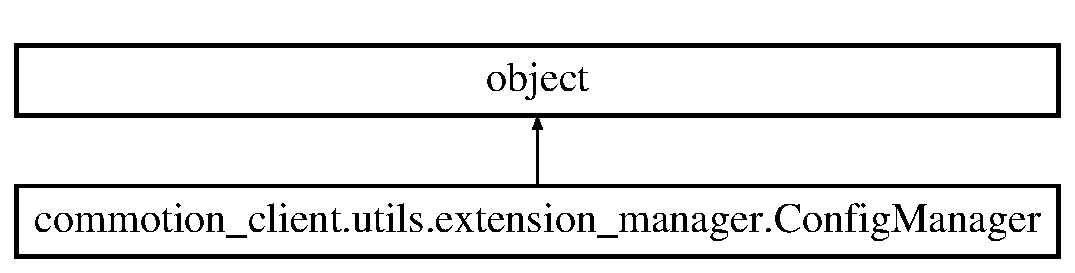
\includegraphics[height=2.000000cm]{classcommotion__client_1_1utils_1_1extension__manager_1_1ConfigManager}
\end{center}
\end{figure}
\subsection*{Public Member Functions}
\begin{DoxyCompactItemize}
\item 
def \hyperlink{classcommotion__client_1_1utils_1_1extension__manager_1_1ConfigManager_a152c0575bbf11ee6c2c1c24e300a7034}{\-\_\-\-\_\-init\-\_\-\-\_\-}
\item 
def \hyperlink{classcommotion__client_1_1utils_1_1extension__manager_1_1ConfigManager_ab8bb11d6b12687d9a7e22953d3125ef9}{has\-\_\-configs}
\item 
def \hyperlink{classcommotion__client_1_1utils_1_1extension__manager_1_1ConfigManager_a540ef57dff72ba46c043abd217e221cf}{find}
\item 
def \hyperlink{classcommotion__client_1_1utils_1_1extension__manager_1_1ConfigManager_ac8075c8f0e46b33f63c4b79f91d2ee3e}{get\-\_\-paths}
\item 
def \hyperlink{classcommotion__client_1_1utils_1_1extension__manager_1_1ConfigManager_aa5d4504ee2b1a228e0543e0bd4313b88}{get}
\item 
def \hyperlink{classcommotion__client_1_1utils_1_1extension__manager_1_1ConfigManager_a3da851319b205bf97e350946b4408ff8}{load}
\end{DoxyCompactItemize}
\subsection*{Public Attributes}
\begin{DoxyCompactItemize}
\item 
\hypertarget{classcommotion__client_1_1utils_1_1extension__manager_1_1ConfigManager_aaf53690e921a06e6b522489b884d184a}{{\bfseries log}}\label{classcommotion__client_1_1utils_1_1extension__manager_1_1ConfigManager_aaf53690e921a06e6b522489b884d184a}

\item 
\hypertarget{classcommotion__client_1_1utils_1_1extension__manager_1_1ConfigManager_aa0ce09aefdd36656f0a1abfad14e9ff1}{{\bfseries translate}}\label{classcommotion__client_1_1utils_1_1extension__manager_1_1ConfigManager_aa0ce09aefdd36656f0a1abfad14e9ff1}

\item 
\hypertarget{classcommotion__client_1_1utils_1_1extension__manager_1_1ConfigManager_a13f7fe6d2a2802b7a74b635aa610ece7}{{\bfseries configs}}\label{classcommotion__client_1_1utils_1_1extension__manager_1_1ConfigManager_a13f7fe6d2a2802b7a74b635aa610ece7}

\item 
\hypertarget{classcommotion__client_1_1utils_1_1extension__manager_1_1ConfigManager_a26693e1c1001c0967fe11876e5b37327}{{\bfseries directory}}\label{classcommotion__client_1_1utils_1_1extension__manager_1_1ConfigManager_a26693e1c1001c0967fe11876e5b37327}

\item 
\hypertarget{classcommotion__client_1_1utils_1_1extension__manager_1_1ConfigManager_a0e2fabb5da2d9be8b5c12aed0e8f3661}{{\bfseries paths}}\label{classcommotion__client_1_1utils_1_1extension__manager_1_1ConfigManager_a0e2fabb5da2d9be8b5c12aed0e8f3661}

\end{DoxyCompactItemize}


\subsection{Detailed Description}
\begin{DoxyVerb}A object for loading config data from a library.

This object should only be used to load configs and saving/checking those values against the users settings. Any value checking should take place in the users settings.
\end{DoxyVerb}
 

\subsection{Constructor \& Destructor Documentation}
\hypertarget{classcommotion__client_1_1utils_1_1extension__manager_1_1ConfigManager_a152c0575bbf11ee6c2c1c24e300a7034}{\index{commotion\-\_\-client\-::utils\-::extension\-\_\-manager\-::\-Config\-Manager@{commotion\-\_\-client\-::utils\-::extension\-\_\-manager\-::\-Config\-Manager}!\-\_\-\-\_\-init\-\_\-\-\_\-@{\-\_\-\-\_\-init\-\_\-\-\_\-}}
\index{\-\_\-\-\_\-init\-\_\-\-\_\-@{\-\_\-\-\_\-init\-\_\-\-\_\-}!commotion_client::utils::extension_manager::ConfigManager@{commotion\-\_\-client\-::utils\-::extension\-\_\-manager\-::\-Config\-Manager}}
\subsubsection[{\-\_\-\-\_\-init\-\_\-\-\_\-}]{\setlength{\rightskip}{0pt plus 5cm}def commotion\-\_\-client.\-utils.\-extension\-\_\-manager.\-Config\-Manager.\-\_\-\-\_\-init\-\_\-\-\_\- (
\begin{DoxyParamCaption}
\item[{}]{self, }
\item[{}]{path = {\ttfamily None}}
\end{DoxyParamCaption}
)}}\label{classcommotion__client_1_1utils_1_1extension__manager_1_1ConfigManager_a152c0575bbf11ee6c2c1c24e300a7034}
\begin{DoxyVerb}Args:
  path (string): The path to an extension library.
\end{DoxyVerb}
 

References commotion\-\_\-client.\-utils.\-extension\-\_\-manager.\-Config\-Manager.\-configs, commotion\-\_\-client.\-utils.\-extension\-\_\-manager.\-Config\-Manager.\-directory, commotion\-\_\-client.\-utils.\-extension\-\_\-manager.\-Config\-Manager.\-get(), commotion\-\_\-client.\-utils.\-extension\-\_\-manager.\-Config\-Manager.\-get\-\_\-paths(), commotion\-\_\-client.\-G\-U\-I.\-system\-\_\-tray.\-Tray\-Icon.\-log, commotion\-\_\-client.\-G\-U\-I.\-welcome\-\_\-page.\-View\-Port.\-log, commotion\-\_\-client.\-G\-U\-I.\-menu\-\_\-bar.\-Menu\-Bar.\-log, commotion\-\_\-client.\-G\-U\-I.\-crash\-\_\-report.\-Crash\-Report.\-log, commotion\-\_\-client.\-extensions.\-config\-\_\-editor.\-main.\-View\-Port.\-log, commotion\-\_\-client.\-G\-U\-I.\-main\-\_\-window.\-Main\-Window.\-log, commotion\-\_\-client.\-G\-U\-I.\-toolbar\-\_\-builder.\-Tool\-Bar.\-log, commotion\-\_\-client.\-G\-U\-I.\-toolbar.\-Tool\-Bar.\-log, commotion\-\_\-client.\-G\-U\-I.\-extension\-\_\-toolbar.\-Extension\-Tool\-Bar.\-log, commotion\-\_\-client.\-utils.\-extension\-\_\-manager.\-Extension\-Manager.\-log, commotion\-\_\-client.\-commotion\-\_\-client.\-Hold\-State\-During\-Restart.\-log, commotion\-\_\-client.\-G\-U\-I.\-extension\-\_\-toolbar.\-Menu\-Item.\-log, commotion\-\_\-client.\-G\-U\-I.\-crash\-\_\-report.\-Report\-Gatherer.\-log, commotion\-\_\-client.\-commotion\-\_\-client.\-Commotion\-Client\-Application.\-log, commotion\-\_\-client.\-utils.\-extension\-\_\-manager.\-Config\-Manager.\-log, commotion\-\_\-client.\-utils.\-extension\-\_\-manager.\-Config\-Manager.\-paths, commotion\-\_\-client.\-G\-U\-I.\-menu\-\_\-bar.\-Menu\-Bar.\-translate, commotion\-\_\-client.\-extensions.\-config\-\_\-editor.\-main.\-View\-Port.\-translate, commotion\-\_\-client.\-G\-U\-I.\-main\-\_\-window.\-Main\-Window.\-translate, commotion\-\_\-client.\-G\-U\-I.\-toolbar\-\_\-builder.\-Tool\-Bar.\-translate, commotion\-\_\-client.\-G\-U\-I.\-extension\-\_\-toolbar.\-Extension\-Tool\-Bar.\-translate, commotion\-\_\-client.\-G\-U\-I.\-toolbar.\-Tool\-Bar.\-translate, commotion\-\_\-client.\-utils.\-extension\-\_\-manager.\-Extension\-Manager.\-translate, commotion\-\_\-client.\-G\-U\-I.\-extension\-\_\-toolbar.\-Menu\-Item.\-translate, commotion\-\_\-client.\-commotion\-\_\-client.\-Commotion\-Client\-Application.\-translate, and commotion\-\_\-client.\-utils.\-extension\-\_\-manager.\-Config\-Manager.\-translate.


\begin{DoxyCode}
622 
623     \textcolor{keyword}{def }\hyperlink{classcommotion__client_1_1utils_1_1extension__manager_1_1ConfigManager_a152c0575bbf11ee6c2c1c24e300a7034}{\_\_init\_\_}(self, path=None):
624         \textcolor{stringliteral}{"""}
625 \textcolor{stringliteral}{        Args:}
626 \textcolor{stringliteral}{          path (string): The path to an extension library.}
627 \textcolor{stringliteral}{        """}
628         \textcolor{comment}{#set function logger}
629         self.\hyperlink{classcommotion__client_1_1utils_1_1extension__manager_1_1ConfigManager_aaf53690e921a06e6b522489b884d184a}{log} = logging.getLogger(\textcolor{stringliteral}{"commotion\_client."}+\_\_name\_\_)
630         self.\hyperlink{classcommotion__client_1_1utils_1_1extension__manager_1_1ConfigManager_aa0ce09aefdd36656f0a1abfad14e9ff1}{translate} = QtCore.QCoreApplication.translate
631         self.log.debug(self.\hyperlink{classcommotion__client_1_1utils_1_1extension__manager_1_1ConfigManager_aa0ce09aefdd36656f0a1abfad14e9ff1}{translate}(\textcolor{stringliteral}{"logs"}, \textcolor{stringliteral}{"Initalizing ConfigManager"}))
632         self.\hyperlink{classcommotion__client_1_1utils_1_1extension__manager_1_1ConfigManager_a13f7fe6d2a2802b7a74b635aa610ece7}{configs} = []
633         self.\hyperlink{classcommotion__client_1_1utils_1_1extension__manager_1_1ConfigManager_a26693e1c1001c0967fe11876e5b37327}{directory} = \textcolor{keywordtype}{None}
634         self.\hyperlink{classcommotion__client_1_1utils_1_1extension__manager_1_1ConfigManager_a0e2fabb5da2d9be8b5c12aed0e8f3661}{paths} = []
635         \textcolor{keywordflow}{if} path:
636             self.\hyperlink{classcommotion__client_1_1utils_1_1extension__manager_1_1ConfigManager_a26693e1c1001c0967fe11876e5b37327}{directory} = path
637             \textcolor{keywordflow}{try}:
638                 self.\hyperlink{classcommotion__client_1_1utils_1_1extension__manager_1_1ConfigManager_a0e2fabb5da2d9be8b5c12aed0e8f3661}{paths} = self.\hyperlink{classcommotion__client_1_1utils_1_1extension__manager_1_1ConfigManager_ac8075c8f0e46b33f63c4b79f91d2ee3e}{get\_paths}(path)
639             \textcolor{keywordflow}{except} TypeError:
640                 self.log.debug(self.\hyperlink{classcommotion__client_1_1utils_1_1extension__manager_1_1ConfigManager_aa0ce09aefdd36656f0a1abfad14e9ff1}{translate}(\textcolor{stringliteral}{"logs"}, \textcolor{stringliteral}{"No extensions found in the \{0\} directory.
       You must first populate the folder with extensions to init a ConfigManager in that folder. You can create a
       ConfigManager without a location specified, but you will have to add extensions before getting paths."}.format
      (path)))
641                 \textcolor{keywordflow}{raise} ValueError(self.\hyperlink{classcommotion__client_1_1utils_1_1extension__manager_1_1ConfigManager_aa0ce09aefdd36656f0a1abfad14e9ff1}{translate}(\textcolor{stringliteral}{"logs"}, \textcolor{stringliteral}{"The path \{0\} is empty. ConfigManager
       could not be created"}.format(path)))
642             \textcolor{keywordflow}{else}:
643                 self.log.info(self.\hyperlink{classcommotion__client_1_1utils_1_1extension__manager_1_1ConfigManager_aa0ce09aefdd36656f0a1abfad14e9ff1}{translate}(\textcolor{stringliteral}{"logs"}, \textcolor{stringliteral}{"Extensions found in the \{0\} directory.
       Attempting to load extension configs."}.format(path)))
644                 self.\hyperlink{classcommotion__client_1_1utils_1_1extension__manager_1_1ConfigManager_a13f7fe6d2a2802b7a74b635aa610ece7}{configs} = list(self.\hyperlink{classcommotion__client_1_1utils_1_1extension__manager_1_1ConfigManager_aa5d4504ee2b1a228e0543e0bd4313b88}{get}())

\end{DoxyCode}


\subsection{Member Function Documentation}
\hypertarget{classcommotion__client_1_1utils_1_1extension__manager_1_1ConfigManager_a540ef57dff72ba46c043abd217e221cf}{\index{commotion\-\_\-client\-::utils\-::extension\-\_\-manager\-::\-Config\-Manager@{commotion\-\_\-client\-::utils\-::extension\-\_\-manager\-::\-Config\-Manager}!find@{find}}
\index{find@{find}!commotion_client::utils::extension_manager::ConfigManager@{commotion\-\_\-client\-::utils\-::extension\-\_\-manager\-::\-Config\-Manager}}
\subsubsection[{find}]{\setlength{\rightskip}{0pt plus 5cm}def commotion\-\_\-client.\-utils.\-extension\-\_\-manager.\-Config\-Manager.\-find (
\begin{DoxyParamCaption}
\item[{}]{self, }
\item[{}]{name = {\ttfamily None}}
\end{DoxyParamCaption}
)}}\label{classcommotion__client_1_1utils_1_1extension__manager_1_1ConfigManager_a540ef57dff72ba46c043abd217e221cf}
\begin{DoxyVerb}Function used to obtain a config file from the ConfigManager.

@param name optional The name of the configuration file if known
@param path string The absolute path to the folder to check for extension configs.

@return list of tuples containing a config name and its config.
\end{DoxyVerb}
 

References commotion\-\_\-client.\-utils.\-extension\-\_\-manager.\-Config\-Manager.\-configs, commotion\-\_\-client.\-G\-U\-I.\-menu\-\_\-bar.\-Menu\-Bar.\-translate, commotion\-\_\-client.\-extensions.\-config\-\_\-editor.\-main.\-View\-Port.\-translate, commotion\-\_\-client.\-G\-U\-I.\-main\-\_\-window.\-Main\-Window.\-translate, commotion\-\_\-client.\-G\-U\-I.\-toolbar\-\_\-builder.\-Tool\-Bar.\-translate, commotion\-\_\-client.\-G\-U\-I.\-extension\-\_\-toolbar.\-Extension\-Tool\-Bar.\-translate, commotion\-\_\-client.\-G\-U\-I.\-toolbar.\-Tool\-Bar.\-translate, commotion\-\_\-client.\-utils.\-extension\-\_\-manager.\-Extension\-Manager.\-translate, commotion\-\_\-client.\-G\-U\-I.\-extension\-\_\-toolbar.\-Menu\-Item.\-translate, commotion\-\_\-client.\-commotion\-\_\-client.\-Commotion\-Client\-Application.\-translate, and commotion\-\_\-client.\-utils.\-extension\-\_\-manager.\-Config\-Manager.\-translate.


\begin{DoxyCode}
656 
657     \textcolor{keyword}{def }\hyperlink{classcommotion__client_1_1utils_1_1extension__manager_1_1ConfigManager_a540ef57dff72ba46c043abd217e221cf}{find}(self, name=None):
658         \textcolor{stringliteral}{"""}
659 \textcolor{stringliteral}{        Function used to obtain a config file from the ConfigManager.}
660 \textcolor{stringliteral}{}
661 \textcolor{stringliteral}{        @param name optional The name of the configuration file if known}
662 \textcolor{stringliteral}{        @param path string The absolute path to the folder to check for extension configs.}
663 \textcolor{stringliteral}{}
664 \textcolor{stringliteral}{        @return list of tuples containing a config name and its config.}
665 \textcolor{stringliteral}{        """}
666         \textcolor{keywordflow}{if} \textcolor{keywordflow}{not} self.\hyperlink{classcommotion__client_1_1utils_1_1extension__manager_1_1ConfigManager_a13f7fe6d2a2802b7a74b635aa610ece7}{configs}:
667             self.log.warning(self.\hyperlink{classcommotion__client_1_1utils_1_1extension__manager_1_1ConfigManager_aa0ce09aefdd36656f0a1abfad14e9ff1}{translate}(\textcolor{stringliteral}{"logs"}, \textcolor{stringliteral}{"No configs have been loaded. Please load
       configs first."}.format(name)))
668             \textcolor{keywordflow}{return} \textcolor{keyword}{False}
669         \textcolor{keywordflow}{if} \textcolor{keywordflow}{not} name:
670             \textcolor{keywordflow}{return} self.\hyperlink{classcommotion__client_1_1utils_1_1extension__manager_1_1ConfigManager_a13f7fe6d2a2802b7a74b635aa610ece7}{configs}
671         \textcolor{keywordflow}{elif} name != \textcolor{keywordtype}{None}:
672             \textcolor{keywordflow}{for} conf \textcolor{keywordflow}{in} self.\hyperlink{classcommotion__client_1_1utils_1_1extension__manager_1_1ConfigManager_a13f7fe6d2a2802b7a74b635aa610ece7}{configs}:
673                 \textcolor{keywordflow}{if} conf[\textcolor{stringliteral}{"name"}] \textcolor{keywordflow}{and} conf[\textcolor{stringliteral}{"name"}] == name:
674                     \textcolor{keywordflow}{return} conf
675             self.log.error(self.\hyperlink{classcommotion__client_1_1utils_1_1extension__manager_1_1ConfigManager_aa0ce09aefdd36656f0a1abfad14e9ff1}{translate}(\textcolor{stringliteral}{"logs"}, \textcolor{stringliteral}{"No config of the chosed type named \{0\} found"}.
      format(name)))
676             \textcolor{keywordflow}{return} \textcolor{keyword}{False}

\end{DoxyCode}
\hypertarget{classcommotion__client_1_1utils_1_1extension__manager_1_1ConfigManager_aa5d4504ee2b1a228e0543e0bd4313b88}{\index{commotion\-\_\-client\-::utils\-::extension\-\_\-manager\-::\-Config\-Manager@{commotion\-\_\-client\-::utils\-::extension\-\_\-manager\-::\-Config\-Manager}!get@{get}}
\index{get@{get}!commotion_client::utils::extension_manager::ConfigManager@{commotion\-\_\-client\-::utils\-::extension\-\_\-manager\-::\-Config\-Manager}}
\subsubsection[{get}]{\setlength{\rightskip}{0pt plus 5cm}def commotion\-\_\-client.\-utils.\-extension\-\_\-manager.\-Config\-Manager.\-get (
\begin{DoxyParamCaption}
\item[{}]{self, }
\item[{}]{paths = {\ttfamily None}}
\end{DoxyParamCaption}
)}}\label{classcommotion__client_1_1utils_1_1extension__manager_1_1ConfigManager_aa5d4504ee2b1a228e0543e0bd4313b88}
\begin{DoxyVerb}Generator to retreive config files for the paths passed to it

@param a list of paths of the configuration file to retreive
@return config file as a dictionary
\end{DoxyVerb}
 

References commotion\-\_\-client.\-utils.\-extension\-\_\-manager.\-Config\-Manager.\-load(), commotion\-\_\-client.\-utils.\-extension\-\_\-manager.\-Config\-Manager.\-paths, commotion\-\_\-client.\-G\-U\-I.\-menu\-\_\-bar.\-Menu\-Bar.\-translate, commotion\-\_\-client.\-extensions.\-config\-\_\-editor.\-main.\-View\-Port.\-translate, commotion\-\_\-client.\-G\-U\-I.\-main\-\_\-window.\-Main\-Window.\-translate, commotion\-\_\-client.\-G\-U\-I.\-toolbar\-\_\-builder.\-Tool\-Bar.\-translate, commotion\-\_\-client.\-G\-U\-I.\-toolbar.\-Tool\-Bar.\-translate, commotion\-\_\-client.\-G\-U\-I.\-extension\-\_\-toolbar.\-Extension\-Tool\-Bar.\-translate, commotion\-\_\-client.\-utils.\-extension\-\_\-manager.\-Extension\-Manager.\-translate, commotion\-\_\-client.\-G\-U\-I.\-extension\-\_\-toolbar.\-Menu\-Item.\-translate, commotion\-\_\-client.\-commotion\-\_\-client.\-Commotion\-Client\-Application.\-translate, and commotion\-\_\-client.\-utils.\-extension\-\_\-manager.\-Config\-Manager.\-translate.



Referenced by commotion\-\_\-client.\-utils.\-extension\-\_\-manager.\-Config\-Manager.\-\_\-\-\_\-init\-\_\-\-\_\-().


\begin{DoxyCode}
719 
720     \textcolor{keyword}{def }\hyperlink{classcommotion__client_1_1utils_1_1extension__manager_1_1ConfigManager_aa5d4504ee2b1a228e0543e0bd4313b88}{get}(self, paths=None):
721         \textcolor{stringliteral}{"""}
722 \textcolor{stringliteral}{        Generator to retreive config files for the paths passed to it}
723 \textcolor{stringliteral}{}
724 \textcolor{stringliteral}{        @param a list of paths of the configuration file to retreive}
725 \textcolor{stringliteral}{        @return config file as a dictionary}
726 \textcolor{stringliteral}{        """}
727         \textcolor{comment}{#load config file}
728         \textcolor{keywordflow}{if} \textcolor{keywordflow}{not} paths:
729             self.log.debug(self.\hyperlink{classcommotion__client_1_1utils_1_1extension__manager_1_1ConfigManager_aa0ce09aefdd36656f0a1abfad14e9ff1}{translate}(\textcolor{stringliteral}{"logs"}, \textcolor{stringliteral}{"No paths found. Attempting to load all
       extension manager paths list."}))
730             paths = self.\hyperlink{classcommotion__client_1_1utils_1_1extension__manager_1_1ConfigManager_a0e2fabb5da2d9be8b5c12aed0e8f3661}{paths}
731             self.log.debug(self.\hyperlink{classcommotion__client_1_1utils_1_1extension__manager_1_1ConfigManager_aa0ce09aefdd36656f0a1abfad14e9ff1}{translate}(\textcolor{stringliteral}{"logs"}, \textcolor{stringliteral}{"Found paths:\{0\}."}.format(paths)))
732         \textcolor{keywordflow}{for} path \textcolor{keywordflow}{in} paths:
733             \textcolor{keywordflow}{if} fs\_utils.is\_file(path):
734                 config = self.\hyperlink{classcommotion__client_1_1utils_1_1extension__manager_1_1ConfigManager_a3da851319b205bf97e350946b4408ff8}{load}(path)
735                 \textcolor{keywordflow}{if} config:
736                     \textcolor{keywordflow}{yield} config
737             \textcolor{keywordflow}{else}:
738                 self.log.warning(self.\hyperlink{classcommotion__client_1_1utils_1_1extension__manager_1_1ConfigManager_aa0ce09aefdd36656f0a1abfad14e9ff1}{translate}(\textcolor{stringliteral}{"logs"}, \textcolor{stringliteral}{"Config file \{0\} does not exist and
       therefore cannot be loaded."}.format(path)))

\end{DoxyCode}
\hypertarget{classcommotion__client_1_1utils_1_1extension__manager_1_1ConfigManager_ac8075c8f0e46b33f63c4b79f91d2ee3e}{\index{commotion\-\_\-client\-::utils\-::extension\-\_\-manager\-::\-Config\-Manager@{commotion\-\_\-client\-::utils\-::extension\-\_\-manager\-::\-Config\-Manager}!get\-\_\-paths@{get\-\_\-paths}}
\index{get\-\_\-paths@{get\-\_\-paths}!commotion_client::utils::extension_manager::ConfigManager@{commotion\-\_\-client\-::utils\-::extension\-\_\-manager\-::\-Config\-Manager}}
\subsubsection[{get\-\_\-paths}]{\setlength{\rightskip}{0pt plus 5cm}def commotion\-\_\-client.\-utils.\-extension\-\_\-manager.\-Config\-Manager.\-get\-\_\-paths (
\begin{DoxyParamCaption}
\item[{}]{self, }
\item[{}]{directory}
\end{DoxyParamCaption}
)}}\label{classcommotion__client_1_1utils_1_1extension__manager_1_1ConfigManager_ac8075c8f0e46b33f63c4b79f91d2ee3e}
\begin{DoxyVerb}Returns the paths to all extensions with config files within a directory.

Args:
  directory (string): The path to the folder that extension's are within. Extensions can be up to one level below the directory given.

Returns:
  config_files (array): An array of paths to all extension objects with config files that were found.

Raises:
  TypeError: If no extensions exist within the directory requested.
  AssertionError: If the directory path does not exist.\end{DoxyVerb}
 

References commotion\-\_\-client.\-G\-U\-I.\-menu\-\_\-bar.\-Menu\-Bar.\-translate, commotion\-\_\-client.\-extensions.\-config\-\_\-editor.\-main.\-View\-Port.\-translate, commotion\-\_\-client.\-G\-U\-I.\-main\-\_\-window.\-Main\-Window.\-translate, commotion\-\_\-client.\-G\-U\-I.\-toolbar\-\_\-builder.\-Tool\-Bar.\-translate, commotion\-\_\-client.\-G\-U\-I.\-toolbar.\-Tool\-Bar.\-translate, commotion\-\_\-client.\-G\-U\-I.\-extension\-\_\-toolbar.\-Extension\-Tool\-Bar.\-translate, commotion\-\_\-client.\-utils.\-extension\-\_\-manager.\-Extension\-Manager.\-translate, commotion\-\_\-client.\-G\-U\-I.\-extension\-\_\-toolbar.\-Menu\-Item.\-translate, commotion\-\_\-client.\-commotion\-\_\-client.\-Commotion\-Client\-Application.\-translate, and commotion\-\_\-client.\-utils.\-extension\-\_\-manager.\-Config\-Manager.\-translate.



Referenced by commotion\-\_\-client.\-utils.\-extension\-\_\-manager.\-Config\-Manager.\-\_\-\-\_\-init\-\_\-\-\_\-().


\begin{DoxyCode}
677 
678     \textcolor{keyword}{def }\hyperlink{classcommotion__client_1_1utils_1_1extension__manager_1_1ConfigManager_ac8075c8f0e46b33f63c4b79f91d2ee3e}{get\_paths}(self, directory):
679         \textcolor{stringliteral}{"""Returns the paths to all extensions with config files within a directory.}
680 \textcolor{stringliteral}{        }
681 \textcolor{stringliteral}{        Args:}
682 \textcolor{stringliteral}{          directory (string): The path to the folder that extension's are within. Extensions can be up to
       one level below the directory given.}
683 \textcolor{stringliteral}{        }
684 \textcolor{stringliteral}{        Returns:}
685 \textcolor{stringliteral}{          config\_files (array): An array of paths to all extension objects with config files that were
       found.}
686 \textcolor{stringliteral}{        }
687 \textcolor{stringliteral}{        Raises:}
688 \textcolor{stringliteral}{          TypeError: If no extensions exist within the directory requested.}
689 \textcolor{stringliteral}{          AssertionError: If the directory path does not exist.}
690 \textcolor{stringliteral}{        }
691 \textcolor{stringliteral}{        """}
692         \textcolor{comment}{#Check the directory and raise value error if not there}
693         dir\_obj = QtCore.QDir(str(directory))
694         \textcolor{keywordflow}{if} \textcolor{keywordflow}{not} dir\_obj.exists(dir\_obj.absolutePath()):
695             \textcolor{keywordflow}{raise} ValueError(self.\hyperlink{classcommotion__client_1_1utils_1_1extension__manager_1_1ConfigManager_aa0ce09aefdd36656f0a1abfad14e9ff1}{translate}(\textcolor{stringliteral}{"logs"}, \textcolor{stringliteral}{"Folder at path \{0\} does not exist. No Config
       files loaded."}.format(str(directory))))
696         \textcolor{keywordflow}{else}:
697             path = dir\_obj.absolutePath()
698 
699         config\_files = []
700         \textcolor{keywordflow}{try}:
701             \textcolor{keywordflow}{for} root, dirs, files \textcolor{keywordflow}{in} fs\_utils.walklevel(path):
702                 \textcolor{keywordflow}{for} file\_name \textcolor{keywordflow}{in} files:
703                     \textcolor{keywordflow}{if} zipfile.is\_zipfile(os.path.join(root, file\_name)):
704                         ext\_zip = zipfile.ZipFile(os.path.join(root, file\_name), \textcolor{stringliteral}{'}\textcolor{stringliteral}{r')}
705 \textcolor{stringliteral}{                        ext\_names = ext\_zip.namelist()}
706 \textcolor{stringliteral}{                        }\textcolor{keywordflow}{for} member\_name \textcolor{keywordflow}{in} ext\_names:
707                             \textcolor{keywordflow}{if} member\_name.endswith(\textcolor{stringliteral}{".conf"}):
708                                 config\_files.append(os.path.join(root, file\_name))
709         \textcolor{keywordflow}{except} AssertionError:
710             self.log.warn(self.\hyperlink{classcommotion__client_1_1utils_1_1extension__manager_1_1ConfigManager_aa0ce09aefdd36656f0a1abfad14e9ff1}{translate}(\textcolor{stringliteral}{"logs"}, \textcolor{stringliteral}{"Extension library at path \{0\} does not exist. No
       Config files identified."}.format(path)))
711             \textcolor{keywordflow}{raise}
712         \textcolor{keywordflow}{except} TypeError:
713             self.log.warn(self.\hyperlink{classcommotion__client_1_1utils_1_1extension__manager_1_1ConfigManager_aa0ce09aefdd36656f0a1abfad14e9ff1}{translate}(\textcolor{stringliteral}{"logs"}, \textcolor{stringliteral}{"No extensions found at path \{0\}. No Config files
       identified."}.format(path)))
714             \textcolor{keywordflow}{raise}
715         \textcolor{keywordflow}{if} config\_files:
716             \textcolor{keywordflow}{return} config\_files
717         \textcolor{keywordflow}{else}:
718             \textcolor{keywordflow}{raise} TypeError(self.\hyperlink{classcommotion__client_1_1utils_1_1extension__manager_1_1ConfigManager_aa0ce09aefdd36656f0a1abfad14e9ff1}{translate}(\textcolor{stringliteral}{"logs"}, \textcolor{stringliteral}{"No config files found at path \{0\}. No Config
       files loaded."}.format(path)))

\end{DoxyCode}
\hypertarget{classcommotion__client_1_1utils_1_1extension__manager_1_1ConfigManager_ab8bb11d6b12687d9a7e22953d3125ef9}{\index{commotion\-\_\-client\-::utils\-::extension\-\_\-manager\-::\-Config\-Manager@{commotion\-\_\-client\-::utils\-::extension\-\_\-manager\-::\-Config\-Manager}!has\-\_\-configs@{has\-\_\-configs}}
\index{has\-\_\-configs@{has\-\_\-configs}!commotion_client::utils::extension_manager::ConfigManager@{commotion\-\_\-client\-::utils\-::extension\-\_\-manager\-::\-Config\-Manager}}
\subsubsection[{has\-\_\-configs}]{\setlength{\rightskip}{0pt plus 5cm}def commotion\-\_\-client.\-utils.\-extension\-\_\-manager.\-Config\-Manager.\-has\-\_\-configs (
\begin{DoxyParamCaption}
\item[{}]{self}
\end{DoxyParamCaption}
)}}\label{classcommotion__client_1_1utils_1_1extension__manager_1_1ConfigManager_ab8bb11d6b12687d9a7e22953d3125ef9}
\begin{DoxyVerb}Provides the status of a ConfigManagers config files.

Returns:
  bool: True, if there are configs. False, if there are no configs currently.
\end{DoxyVerb}
 

References commotion\-\_\-client.\-utils.\-extension\-\_\-manager.\-Config\-Manager.\-configs.


\begin{DoxyCode}
645 
646     \textcolor{keyword}{def }\hyperlink{classcommotion__client_1_1utils_1_1extension__manager_1_1ConfigManager_ab8bb11d6b12687d9a7e22953d3125ef9}{has\_configs}(self):
647         \textcolor{stringliteral}{"""Provides the status of a ConfigManagers config files.}
648 \textcolor{stringliteral}{        }
649 \textcolor{stringliteral}{        Returns:}
650 \textcolor{stringliteral}{          bool: True, if there are configs. False, if there are no configs currently.}
651 \textcolor{stringliteral}{        """}
652         \textcolor{keywordflow}{if} self.\hyperlink{classcommotion__client_1_1utils_1_1extension__manager_1_1ConfigManager_a13f7fe6d2a2802b7a74b635aa610ece7}{configs}:
653             \textcolor{keywordflow}{return} \textcolor{keyword}{True}
654         \textcolor{keywordflow}{else}:
655             \textcolor{keywordflow}{return} \textcolor{keyword}{False}
            
\end{DoxyCode}
\hypertarget{classcommotion__client_1_1utils_1_1extension__manager_1_1ConfigManager_a3da851319b205bf97e350946b4408ff8}{\index{commotion\-\_\-client\-::utils\-::extension\-\_\-manager\-::\-Config\-Manager@{commotion\-\_\-client\-::utils\-::extension\-\_\-manager\-::\-Config\-Manager}!load@{load}}
\index{load@{load}!commotion_client::utils::extension_manager::ConfigManager@{commotion\-\_\-client\-::utils\-::extension\-\_\-manager\-::\-Config\-Manager}}
\subsubsection[{load}]{\setlength{\rightskip}{0pt plus 5cm}def commotion\-\_\-client.\-utils.\-extension\-\_\-manager.\-Config\-Manager.\-load (
\begin{DoxyParamCaption}
\item[{}]{self, }
\item[{}]{path}
\end{DoxyParamCaption}
)}}\label{classcommotion__client_1_1utils_1_1extension__manager_1_1ConfigManager_a3da851319b205bf97e350946b4408ff8}
\begin{DoxyVerb}This function loads the formatted config file and returns it.

long description

Args:
path (string): The path to a config file

Returns:
  (dictionary) On success returns a dictionary containing the config file values.
  (bool): On failure returns False\end{DoxyVerb}
 

References commotion\-\_\-client.\-G\-U\-I.\-menu\-\_\-bar.\-Menu\-Bar.\-translate, commotion\-\_\-client.\-extensions.\-config\-\_\-editor.\-main.\-View\-Port.\-translate, commotion\-\_\-client.\-G\-U\-I.\-main\-\_\-window.\-Main\-Window.\-translate, commotion\-\_\-client.\-G\-U\-I.\-toolbar\-\_\-builder.\-Tool\-Bar.\-translate, commotion\-\_\-client.\-G\-U\-I.\-toolbar.\-Tool\-Bar.\-translate, commotion\-\_\-client.\-G\-U\-I.\-extension\-\_\-toolbar.\-Extension\-Tool\-Bar.\-translate, commotion\-\_\-client.\-utils.\-extension\-\_\-manager.\-Extension\-Manager.\-translate, commotion\-\_\-client.\-G\-U\-I.\-extension\-\_\-toolbar.\-Menu\-Item.\-translate, commotion\-\_\-client.\-commotion\-\_\-client.\-Commotion\-Client\-Application.\-translate, and commotion\-\_\-client.\-utils.\-extension\-\_\-manager.\-Config\-Manager.\-translate.



Referenced by commotion\-\_\-client.\-utils.\-extension\-\_\-manager.\-Config\-Manager.\-get().


\begin{DoxyCode}
739 
740     \textcolor{keyword}{def }\hyperlink{classcommotion__client_1_1utils_1_1extension__manager_1_1ConfigManager_a3da851319b205bf97e350946b4408ff8}{load}(self, path):
741         \textcolor{stringliteral}{"""This function loads the formatted config file and returns it.}
742 \textcolor{stringliteral}{        }
743 \textcolor{stringliteral}{        long description}
744 \textcolor{stringliteral}{        }
745 \textcolor{stringliteral}{        Args:}
746 \textcolor{stringliteral}{        path (string): The path to a config file}
747 \textcolor{stringliteral}{        }
748 \textcolor{stringliteral}{        Returns:}
749 \textcolor{stringliteral}{          (dictionary) On success returns a dictionary containing the config file values.}
750 \textcolor{stringliteral}{          (bool): On failure returns False}
751 \textcolor{stringliteral}{        }
752 \textcolor{stringliteral}{        """}
753         config = \textcolor{keywordtype}{None}
754         data = \textcolor{keywordtype}{None}
755         myfile = QtCore.QFile(str(path))
756         \textcolor{keywordflow}{if} \textcolor{keywordflow}{not} myfile.exists():
757             \textcolor{keywordflow}{return} \textcolor{keyword}{False}
758         \textcolor{keywordflow}{if} \textcolor{keywordflow}{not} zipfile.is\_zipfile(str(path)):
759             \textcolor{keywordflow}{return} \textcolor{keyword}{False}
760         with zipfile.ZipFile(path, \textcolor{stringliteral}{'}\textcolor{stringliteral}{r') as zip\_ext:}
761 \textcolor{stringliteral}{            }\textcolor{keywordflow}{for} file\_name \textcolor{keywordflow}{in} zip\_ext.namelist():
762                 \textcolor{keywordflow}{if} file\_name.endswith(\textcolor{stringliteral}{".conf"}):
763                     config = zip\_ext.read(file\_name)
764                     self.log.debug(self.\hyperlink{classcommotion__client_1_1utils_1_1extension__manager_1_1ConfigManager_aa0ce09aefdd36656f0a1abfad14e9ff1}{translate}(\textcolor{stringliteral}{"logs"}, \textcolor{stringliteral}{"Config found in extension \{0\}."}.format(
      path)))
765         \textcolor{keywordflow}{if} config:
766             \textcolor{keywordflow}{try}:
767                 data = json.loads(config.decode(\textcolor{stringliteral}{'utf-8'}))
768                 self.log.info(self.\hyperlink{classcommotion__client_1_1utils_1_1extension__manager_1_1ConfigManager_aa0ce09aefdd36656f0a1abfad14e9ff1}{translate}(\textcolor{stringliteral}{"logs"}, \textcolor{stringliteral}{"Successfully loaded \{0\}'s config file."}.
      format(path)))
769             \textcolor{keywordflow}{except} ValueError:
770                 self.log.warning(self.\hyperlink{classcommotion__client_1_1utils_1_1extension__manager_1_1ConfigManager_aa0ce09aefdd36656f0a1abfad14e9ff1}{translate}(\textcolor{stringliteral}{"logs"}, \textcolor{stringliteral}{"Failed to load \{0\} due to a non-json or
       otherwise invalid file type"}.format(path)))
771                 \textcolor{keywordflow}{return} \textcolor{keyword}{False}
772         \textcolor{keywordflow}{if} data:
773             self.log.debug(self.\hyperlink{classcommotion__client_1_1utils_1_1extension__manager_1_1ConfigManager_aa0ce09aefdd36656f0a1abfad14e9ff1}{translate}(\textcolor{stringliteral}{"logs"}, \textcolor{stringliteral}{"Config file loaded."}.format(path)))
774             \textcolor{keywordflow}{return} data
775         \textcolor{keywordflow}{else}:
776             self.log.debug(self.\hyperlink{classcommotion__client_1_1utils_1_1extension__manager_1_1ConfigManager_aa0ce09aefdd36656f0a1abfad14e9ff1}{translate}(\textcolor{stringliteral}{"logs"}, \textcolor{stringliteral}{"Failed to load config file."}.format(path)))
777             \textcolor{keywordflow}{return} \textcolor{keyword}{False}
\end{DoxyCode}


The documentation for this class was generated from the following file\-:\begin{DoxyCompactItemize}
\item 
commotion\-\_\-client/utils/extension\-\_\-manager.\-py\end{DoxyCompactItemize}

\hypertarget{classtests_1_1utils_1_1extension__manager__tests_1_1ConfigManagerTests}{\section{tests.\-utils.\-extension\-\_\-manager\-\_\-tests.\-Config\-Manager\-Tests Class Reference}
\label{classtests_1_1utils_1_1extension__manager__tests_1_1ConfigManagerTests}\index{tests.\-utils.\-extension\-\_\-manager\-\_\-tests.\-Config\-Manager\-Tests@{tests.\-utils.\-extension\-\_\-manager\-\_\-tests.\-Config\-Manager\-Tests}}
}
Inheritance diagram for tests.\-utils.\-extension\-\_\-manager\-\_\-tests.\-Config\-Manager\-Tests\-:\begin{figure}[H]
\begin{center}
\leavevmode
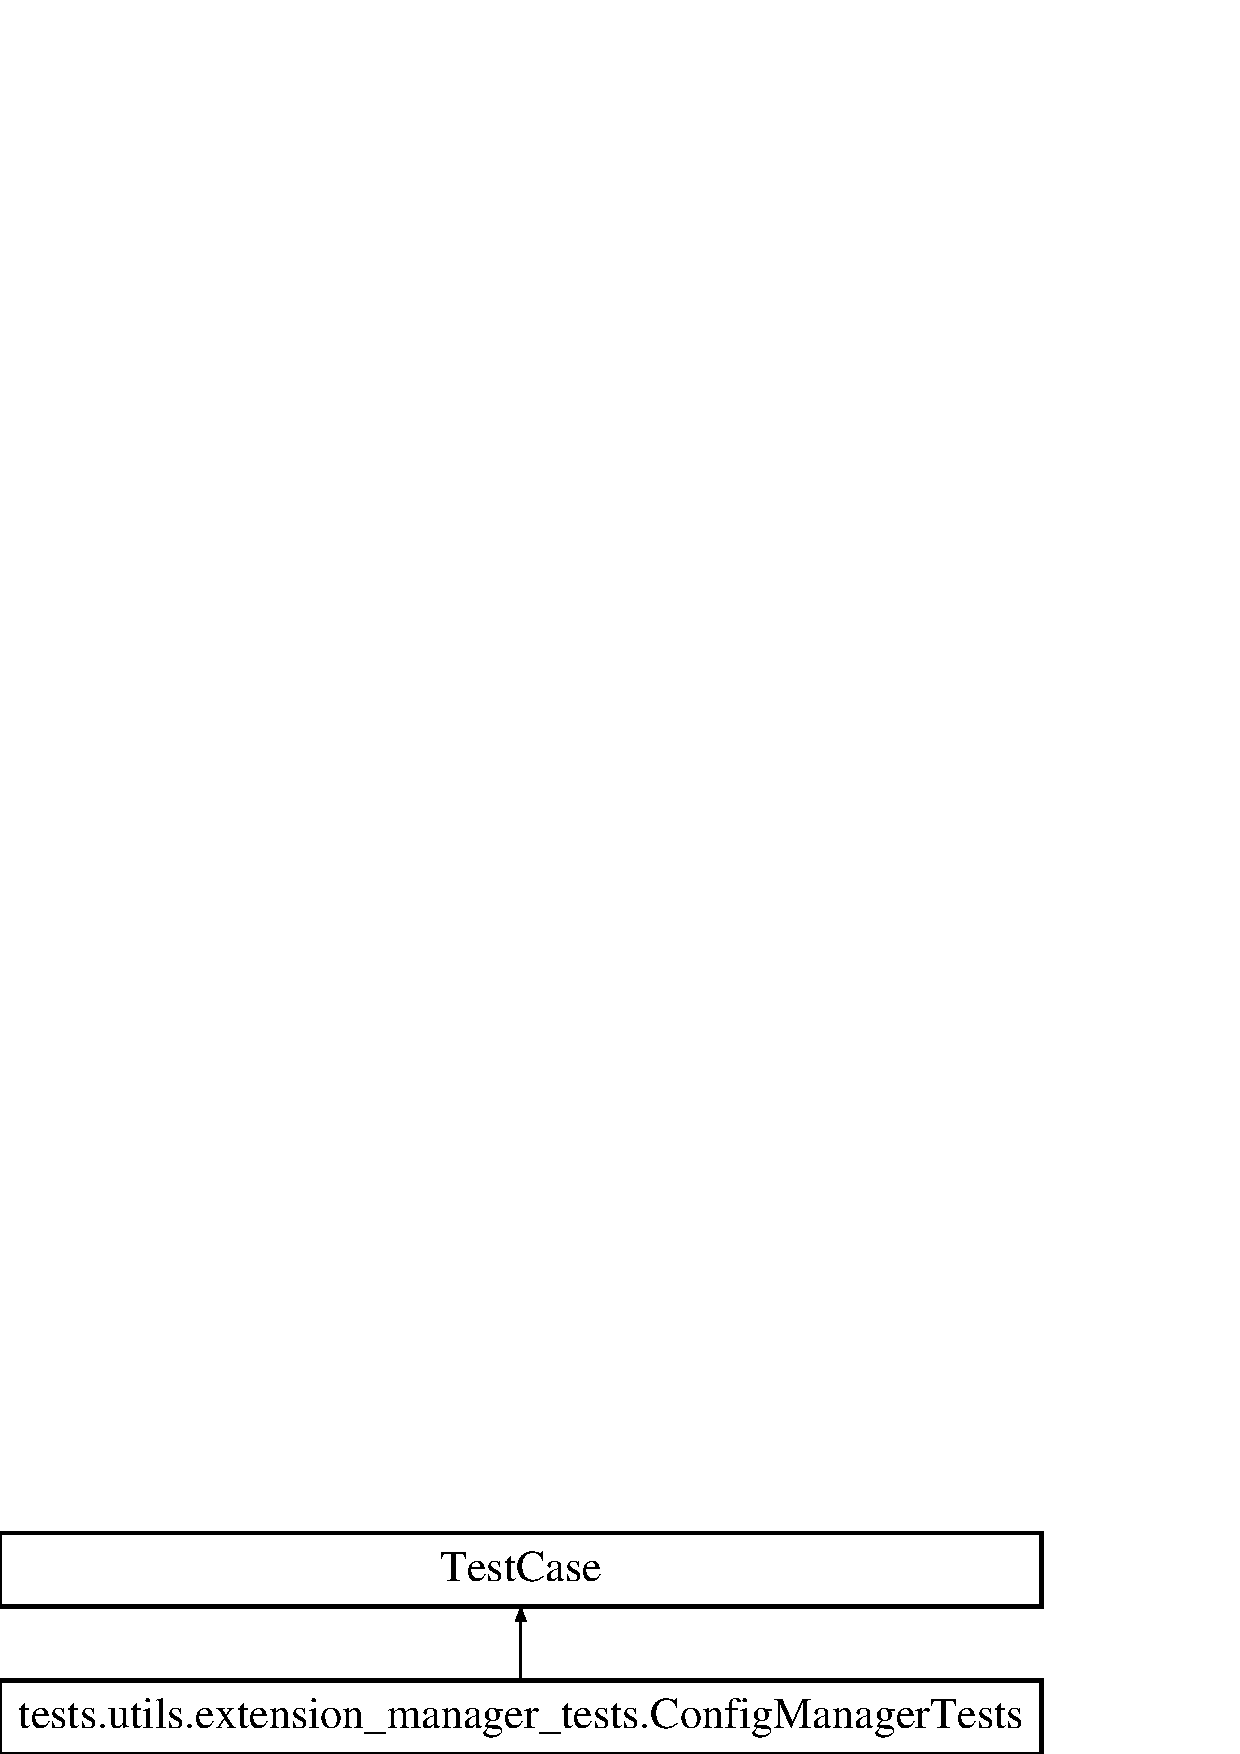
\includegraphics[height=2.000000cm]{classtests_1_1utils_1_1extension__manager__tests_1_1ConfigManagerTests}
\end{center}
\end{figure}
\subsection*{Public Member Functions}
\begin{DoxyCompactItemize}
\item 
\hypertarget{classtests_1_1utils_1_1extension__manager__tests_1_1ConfigManagerTests_a905bba42ed8d2a710c3df445bb90d3ec}{def {\bfseries set\-Up}}\label{classtests_1_1utils_1_1extension__manager__tests_1_1ConfigManagerTests_a905bba42ed8d2a710c3df445bb90d3ec}

\item 
\hypertarget{classtests_1_1utils_1_1extension__manager__tests_1_1ConfigManagerTests_ace0a1571b96d7546fb114815a494cf15}{def {\bfseries tear\-Down}}\label{classtests_1_1utils_1_1extension__manager__tests_1_1ConfigManagerTests_ace0a1571b96d7546fb114815a494cf15}

\item 
\hypertarget{classtests_1_1utils_1_1extension__manager__tests_1_1ConfigManagerTests_a5c9c1b724775243f55487142bf6e8a22}{def {\bfseries test\-\_\-init}}\label{classtests_1_1utils_1_1extension__manager__tests_1_1ConfigManagerTests_a5c9c1b724775243f55487142bf6e8a22}

\item 
\hypertarget{classtests_1_1utils_1_1extension__manager__tests_1_1ConfigManagerTests_a98d36d8d008d43a761acdf3c60d8fd3f}{def {\bfseries test\-\_\-has\-\_\-configs}}\label{classtests_1_1utils_1_1extension__manager__tests_1_1ConfigManagerTests_a98d36d8d008d43a761acdf3c60d8fd3f}

\item 
\hypertarget{classtests_1_1utils_1_1extension__manager__tests_1_1ConfigManagerTests_add838e255cd11c84ebe6205ee5217ddf}{def {\bfseries test\-\_\-find}}\label{classtests_1_1utils_1_1extension__manager__tests_1_1ConfigManagerTests_add838e255cd11c84ebe6205ee5217ddf}

\item 
\hypertarget{classtests_1_1utils_1_1extension__manager__tests_1_1ConfigManagerTests_a7df6a035707a2eaf3b56dc3a180a8629}{def {\bfseries test\-\_\-get\-\_\-path}}\label{classtests_1_1utils_1_1extension__manager__tests_1_1ConfigManagerTests_a7df6a035707a2eaf3b56dc3a180a8629}

\item 
\hypertarget{classtests_1_1utils_1_1extension__manager__tests_1_1ConfigManagerTests_ad9aa64684ceedfbbf65b3ba1861f0415}{def {\bfseries test\-\_\-get}}\label{classtests_1_1utils_1_1extension__manager__tests_1_1ConfigManagerTests_ad9aa64684ceedfbbf65b3ba1861f0415}

\item 
\hypertarget{classtests_1_1utils_1_1extension__manager__tests_1_1ConfigManagerTests_a4d3a4d4fafac03cbf408efb2e34d71ca}{def {\bfseries test\-\_\-load}}\label{classtests_1_1utils_1_1extension__manager__tests_1_1ConfigManagerTests_a4d3a4d4fafac03cbf408efb2e34d71ca}

\end{DoxyCompactItemize}
\subsection*{Public Attributes}
\begin{DoxyCompactItemize}
\item 
\hypertarget{classtests_1_1utils_1_1extension__manager__tests_1_1ConfigManagerTests_af67e4d12f4575bda0b3d25dda63e2ea5}{{\bfseries app}}\label{classtests_1_1utils_1_1extension__manager__tests_1_1ConfigManagerTests_af67e4d12f4575bda0b3d25dda63e2ea5}

\item 
\hypertarget{classtests_1_1utils_1_1extension__manager__tests_1_1ConfigManagerTests_aae5dc5cd86e14b07f1d8b3713d5fa8f4}{{\bfseries econfig}}\label{classtests_1_1utils_1_1extension__manager__tests_1_1ConfigManagerTests_aae5dc5cd86e14b07f1d8b3713d5fa8f4}

\item 
\hypertarget{classtests_1_1utils_1_1extension__manager__tests_1_1ConfigManagerTests_ab5f46c854c44437f5150817e006559d7}{{\bfseries full\-\_\-config}}\label{classtests_1_1utils_1_1extension__manager__tests_1_1ConfigManagerTests_ab5f46c854c44437f5150817e006559d7}

\item 
\hypertarget{classtests_1_1utils_1_1extension__manager__tests_1_1ConfigManagerTests_a0f46e46f16faf60274370dde12326477}{{\bfseries empty\-\_\-config}}\label{classtests_1_1utils_1_1extension__manager__tests_1_1ConfigManagerTests_a0f46e46f16faf60274370dde12326477}

\end{DoxyCompactItemize}


The documentation for this class was generated from the following file\-:\begin{DoxyCompactItemize}
\item 
tests/utils/extension\-\_\-manager\-\_\-tests.\-py\end{DoxyCompactItemize}

\hypertarget{classcommotion__client_1_1GUI_1_1crash__report_1_1CrashReport}{\section{commotion\+\_\+client.\+G\+U\+I.\+crash\+\_\+report.\+Crash\+Report Class Reference}
\label{classcommotion__client_1_1GUI_1_1crash__report_1_1CrashReport}\index{commotion\+\_\+client.\+G\+U\+I.\+crash\+\_\+report.\+Crash\+Report@{commotion\+\_\+client.\+G\+U\+I.\+crash\+\_\+report.\+Crash\+Report}}
}
Inheritance diagram for commotion\+\_\+client.\+G\+U\+I.\+crash\+\_\+report.\+Crash\+Report\+:\begin{figure}[H]
\begin{center}
\leavevmode
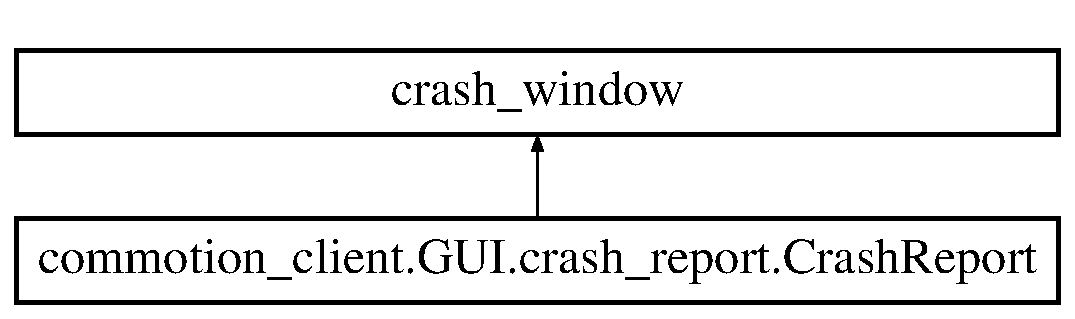
\includegraphics[height=2.000000cm]{classcommotion__client_1_1GUI_1_1crash__report_1_1CrashReport}
\end{center}
\end{figure}
\subsection*{Public Member Functions}
\begin{DoxyCompactItemize}
\item 
\hypertarget{classcommotion__client_1_1GUI_1_1crash__report_1_1CrashReport_a6f0de53cc023adbd4d5c2f01f7e88911}{def {\bfseries \+\_\+\+\_\+init\+\_\+\+\_\+}}\label{classcommotion__client_1_1GUI_1_1crash__report_1_1CrashReport_a6f0de53cc023adbd4d5c2f01f7e88911}

\item 
\hypertarget{classcommotion__client_1_1GUI_1_1crash__report_1_1CrashReport_a58b432a5a1099f015292e059ef2dd13f}{def {\bfseries crash\+\_\+alert}}\label{classcommotion__client_1_1GUI_1_1crash__report_1_1CrashReport_a58b432a5a1099f015292e059ef2dd13f}

\item 
\hypertarget{classcommotion__client_1_1GUI_1_1crash__report_1_1CrashReport_ab188170081888dab4c7998ed405346bc}{def {\bfseries check\+\_\+restart}}\label{classcommotion__client_1_1GUI_1_1crash__report_1_1CrashReport_ab188170081888dab4c7998ed405346bc}

\item 
\hypertarget{classcommotion__client_1_1GUI_1_1crash__report_1_1CrashReport_aa28751948f38f6387a60bb7c5dee13a1}{def {\bfseries check\+\_\+quit}}\label{classcommotion__client_1_1GUI_1_1crash__report_1_1CrashReport_aa28751948f38f6387a60bb7c5dee13a1}

\item 
\hypertarget{classcommotion__client_1_1GUI_1_1crash__report_1_1CrashReport_a996e351321541c30440a64bec91fd973}{def {\bfseries generate\+\_\+report}}\label{classcommotion__client_1_1GUI_1_1crash__report_1_1CrashReport_a996e351321541c30440a64bec91fd973}

\item 
def \hyperlink{classcommotion__client_1_1GUI_1_1crash__report_1_1CrashReport_a04eab1fb6f464494b49a31267f1b48cc}{update\+\_\+countdown}
\item 
def \hyperlink{classcommotion__client_1_1GUI_1_1crash__report_1_1CrashReport_ade1514cafdc6eabee38a3f4cc2468411}{set\+\_\+report}
\item 
def \hyperlink{classcommotion__client_1_1GUI_1_1crash__report_1_1CrashReport_a149cd78e935504d1abc27e4d29a36d67}{save\+\_\+report}
\item 
\hypertarget{classcommotion__client_1_1GUI_1_1crash__report_1_1CrashReport_a0c7f4cec8d06314fc3b83e88fa980a79}{def {\bfseries create\+\_\+uuid}}\label{classcommotion__client_1_1GUI_1_1crash__report_1_1CrashReport_a0c7f4cec8d06314fc3b83e88fa980a79}

\end{DoxyCompactItemize}
\subsection*{Public Attributes}
\begin{DoxyCompactItemize}
\item 
\hypertarget{classcommotion__client_1_1GUI_1_1crash__report_1_1CrashReport_a9ba153801ab8b157b280b13b629ade5f}{{\bfseries log}}\label{classcommotion__client_1_1GUI_1_1crash__report_1_1CrashReport_a9ba153801ab8b157b280b13b629ade5f}

\item 
\hypertarget{classcommotion__client_1_1GUI_1_1crash__report_1_1CrashReport_a30029f0eadda618776981bd6ce3da457}{{\bfseries report\+\_\+timer}}\label{classcommotion__client_1_1GUI_1_1crash__report_1_1CrashReport_a30029f0eadda618776981bd6ce3da457}

\item 
\hypertarget{classcommotion__client_1_1GUI_1_1crash__report_1_1CrashReport_aa15591cfd0396c1ed2a394f5bd26c260}{{\bfseries error\+\_\+msg}}\label{classcommotion__client_1_1GUI_1_1crash__report_1_1CrashReport_aa15591cfd0396c1ed2a394f5bd26c260}

\item 
\hypertarget{classcommotion__client_1_1GUI_1_1crash__report_1_1CrashReport_afb588169ff72c1295594bde3fc80b446}{{\bfseries gatherer}}\label{classcommotion__client_1_1GUI_1_1crash__report_1_1CrashReport_afb588169ff72c1295594bde3fc80b446}

\item 
\hypertarget{classcommotion__client_1_1GUI_1_1crash__report_1_1CrashReport_ad4c1d4ecb077eb73f8048a6d437db8c5}{{\bfseries countdown}}\label{classcommotion__client_1_1GUI_1_1crash__report_1_1CrashReport_ad4c1d4ecb077eb73f8048a6d437db8c5}

\item 
\hypertarget{classcommotion__client_1_1GUI_1_1crash__report_1_1CrashReport_aa7ed5448d9f87f327af863a87fcee52e}{{\bfseries countdown\+\_\+timer}}\label{classcommotion__client_1_1GUI_1_1crash__report_1_1CrashReport_aa7ed5448d9f87f327af863a87fcee52e}

\item 
\hypertarget{classcommotion__client_1_1GUI_1_1crash__report_1_1CrashReport_ae827ad1a3c91a32bb0a588b18d8a6ff2}{{\bfseries compiled\+\_\+report}}\label{classcommotion__client_1_1GUI_1_1crash__report_1_1CrashReport_ae827ad1a3c91a32bb0a588b18d8a6ff2}

\item 
\hypertarget{classcommotion__client_1_1GUI_1_1crash__report_1_1CrashReport_a5edce7f1ad57c34e572afc88a491811f}{{\bfseries uuid}}\label{classcommotion__client_1_1GUI_1_1crash__report_1_1CrashReport_a5edce7f1ad57c34e572afc88a491811f}

\end{DoxyCompactItemize}
\subsection*{Static Public Attributes}
\begin{DoxyCompactItemize}
\item 
\hypertarget{classcommotion__client_1_1GUI_1_1crash__report_1_1CrashReport_affcf604f03f2a94b3732309acb6f597c}{tuple {\bfseries crash\+\_\+override} = Qt\+Core.\+pyqt\+Signal()}\label{classcommotion__client_1_1GUI_1_1crash__report_1_1CrashReport_affcf604f03f2a94b3732309acb6f597c}

\item 
\hypertarget{classcommotion__client_1_1GUI_1_1crash__report_1_1CrashReport_a90c6385d778d37da521af4973b829e21}{tuple {\bfseries crash\+\_\+info} = Qt\+Core.\+pyqt\+Signal(str, dict)}\label{classcommotion__client_1_1GUI_1_1crash__report_1_1CrashReport_a90c6385d778d37da521af4973b829e21}

\item 
\hypertarget{classcommotion__client_1_1GUI_1_1crash__report_1_1CrashReport_a9548f4b6174854f4983cfd0e68ba6202}{tuple {\bfseries crash} = Qt\+Core.\+pyqt\+Signal(str)}\label{classcommotion__client_1_1GUI_1_1crash__report_1_1CrashReport_a9548f4b6174854f4983cfd0e68ba6202}

\item 
\hypertarget{classcommotion__client_1_1GUI_1_1crash__report_1_1CrashReport_a68be7b212539543bd791634b7f2d708a}{tuple {\bfseries alert\+\_\+user} = Qt\+Core.\+pyqt\+Signal(str)}\label{classcommotion__client_1_1GUI_1_1crash__report_1_1CrashReport_a68be7b212539543bd791634b7f2d708a}

\end{DoxyCompactItemize}


\subsection{Member Function Documentation}
\hypertarget{classcommotion__client_1_1GUI_1_1crash__report_1_1CrashReport_a149cd78e935504d1abc27e4d29a36d67}{\index{commotion\+\_\+client\+::\+G\+U\+I\+::crash\+\_\+report\+::\+Crash\+Report@{commotion\+\_\+client\+::\+G\+U\+I\+::crash\+\_\+report\+::\+Crash\+Report}!save\+\_\+report@{save\+\_\+report}}
\index{save\+\_\+report@{save\+\_\+report}!commotion\+\_\+client\+::\+G\+U\+I\+::crash\+\_\+report\+::\+Crash\+Report@{commotion\+\_\+client\+::\+G\+U\+I\+::crash\+\_\+report\+::\+Crash\+Report}}
\subsubsection[{save\+\_\+report}]{\setlength{\rightskip}{0pt plus 5cm}def commotion\+\_\+client.\+G\+U\+I.\+crash\+\_\+report.\+Crash\+Report.\+save\+\_\+report (
\begin{DoxyParamCaption}
\item[{}]{self}
\end{DoxyParamCaption}
)}}\label{classcommotion__client_1_1GUI_1_1crash__report_1_1CrashReport_a149cd78e935504d1abc27e4d29a36d67}
\begin{DoxyVerb}TODO ADD python-gnupg encryption to all data saved here.
\end{DoxyVerb}
 

References commotion\+\_\+client.\+G\+U\+I.\+crash\+\_\+report.\+Crash\+Report.\+compiled\+\_\+report, and commotion\+\_\+client.\+G\+U\+I.\+crash\+\_\+report.\+Crash\+Report.\+uuid.


\begin{DoxyCode}
130 
131     \textcolor{keyword}{def }\hyperlink{classcommotion__client_1_1GUI_1_1crash__report_1_1CrashReport_a149cd78e935504d1abc27e4d29a36d67}{save\_report}(self):
132         \textcolor{stringliteral}{"""}
133 \textcolor{stringliteral}{        TODO ADD python-gnupg encryption to all data saved here.}
134 \textcolor{stringliteral}{        """}
135         \textcolor{comment}{#Save user comments}
136         \textcolor{keywordflow}{try}:
137             self.\hyperlink{classcommotion__client_1_1GUI_1_1crash__report_1_1CrashReport_ae827ad1a3c91a32bb0a588b18d8a6ff2}{compiled\_report}[\textcolor{stringliteral}{'error'}][\textcolor{stringliteral}{'comments'}] = str(self.comment\_field.toPlainText()
      )
138         \textcolor{keywordflow}{except} Exception \textcolor{keyword}{as} e:
139             self.log.info(QtCore.QCoreApplication.translate(\textcolor{stringliteral}{"logs"}, \textcolor{stringliteral}{"The crash reporter could not store
       user comments in the crash report."}))
140             self.log.debug(e, exc\_info=1)
141         \_settings = QtCore.QSettings()
142         \_settings.beginGroup(\textcolor{stringliteral}{"CrashReport/"}+self.\hyperlink{classcommotion__client_1_1GUI_1_1crash__report_1_1CrashReport_a5edce7f1ad57c34e572afc88a491811f}{uuid}) \textcolor{comment}{#create a unique crash report}
143         \textcolor{keywordflow}{for} section, results \textcolor{keywordflow}{in} self.compiled\_report.items():
144             \textcolor{keywordflow}{for} name, value \textcolor{keywordflow}{in} results.items():
145                 \_settings.setValue(section+\textcolor{stringliteral}{"/"}+name, value)
146         \_settings.endGroup()

\end{DoxyCode}
\hypertarget{classcommotion__client_1_1GUI_1_1crash__report_1_1CrashReport_ade1514cafdc6eabee38a3f4cc2468411}{\index{commotion\+\_\+client\+::\+G\+U\+I\+::crash\+\_\+report\+::\+Crash\+Report@{commotion\+\_\+client\+::\+G\+U\+I\+::crash\+\_\+report\+::\+Crash\+Report}!set\+\_\+report@{set\+\_\+report}}
\index{set\+\_\+report@{set\+\_\+report}!commotion\+\_\+client\+::\+G\+U\+I\+::crash\+\_\+report\+::\+Crash\+Report@{commotion\+\_\+client\+::\+G\+U\+I\+::crash\+\_\+report\+::\+Crash\+Report}}
\subsubsection[{set\+\_\+report}]{\setlength{\rightskip}{0pt plus 5cm}def commotion\+\_\+client.\+G\+U\+I.\+crash\+\_\+report.\+Crash\+Report.\+set\+\_\+report (
\begin{DoxyParamCaption}
\item[{}]{self}
\end{DoxyParamCaption}
)}}\label{classcommotion__client_1_1GUI_1_1crash__report_1_1CrashReport_ade1514cafdc6eabee38a3f4cc2468411}
\begin{DoxyVerb}set_report creates and saves the current error report and then disconnects crash_info signal.
\end{DoxyVerb}
 

References commotion\+\_\+client.\+G\+U\+I.\+crash\+\_\+report.\+Crash\+Report.\+compiled\+\_\+report.



Referenced by commotion\+\_\+client.\+G\+U\+I.\+crash\+\_\+report.\+Crash\+Report.\+update\+\_\+countdown().


\begin{DoxyCode}
101 
102     \textcolor{keyword}{def }\hyperlink{classcommotion__client_1_1GUI_1_1crash__report_1_1CrashReport_ade1514cafdc6eabee38a3f4cc2468411}{set\_report}(self):
103         \textcolor{stringliteral}{"""}
104 \textcolor{stringliteral}{        set\_report creates and saves the current error report and then disconnects crash\_info signal.}
105 \textcolor{stringliteral}{        """}
106         \textcolor{comment}{#turn off report gatherer}
107         self.crash\_info.disconnect()
108         \textcolor{keywordflow}{try}:
109             self.\hyperlink{classcommotion__client_1_1GUI_1_1crash__report_1_1CrashReport_ae827ad1a3c91a32bb0a588b18d8a6ff2}{compiled\_report} = self.gatherer.get\_report()
110         \textcolor{keywordflow}{except} Exception \textcolor{keyword}{as} e:
111             self.log.error(QtCore.QCoreApplication.translate(\textcolor{stringliteral}{"logs"}, \textcolor{stringliteral}{"Faile to create a crash report."}))
112             self.log.debug(e, exc\_info=1)
113             self.crash\_report.setPlainText(QtCore.QCoreApplication.translate(\textcolor{stringliteral}{"A crash report could not be
       generated."}))
114             \textcolor{keywordflow}{return}
115         \textcolor{keywordflow}{else}:
116             \textcolor{comment}{#send to user if window activated}
117             printable\_report = []
118             \textcolor{keywordflow}{try}:
119                 \textcolor{keywordflow}{for} section, results \textcolor{keywordflow}{in} self.compiled\_report.items():
120                     printable\_report.append(\textcolor{stringliteral}{"\(\backslash\)n==========  "}+section+\textcolor{stringliteral}{"  ==========\(\backslash\)n"})
121                     \textcolor{comment}{#format and append each name-value pair to the report.}
122                     printable\_report.append(\textcolor{stringliteral}{"\(\backslash\)n"}.join([\textcolor{stringliteral}{'%s = %s'} %(name, value) \textcolor{keywordflow}{for} name, value \textcolor{keywordflow}{in} 
      results.items()]))
123             \textcolor{keywordflow}{except} Exception \textcolor{keyword}{as} e:
124                 self.log.error(QtCore.QCoreApplication.translate(\textcolor{stringliteral}{"logs"}, \textcolor{stringliteral}{"Failed to format crash report for
       user to view."}))
125                 self.log.debug(e, exc\_info=1)
126                 self.crash\_report.setPlainText(QtCore.QCoreApplication.translate(\textcolor{stringliteral}{"Unable to parse crash
       report for viewing. You can send the report without viewing it or un-check \(\backslash\)"Send crash report\(\backslash\)" to cancel
       sending this report."}))
127             \textcolor{keywordflow}{else}:
128                 self.crash\_report.setPlainText(\textcolor{stringliteral}{"\(\backslash\)n"}.join(printable\_report))
129                 \textcolor{comment}{#todo add logs}

\end{DoxyCode}
\hypertarget{classcommotion__client_1_1GUI_1_1crash__report_1_1CrashReport_a04eab1fb6f464494b49a31267f1b48cc}{\index{commotion\+\_\+client\+::\+G\+U\+I\+::crash\+\_\+report\+::\+Crash\+Report@{commotion\+\_\+client\+::\+G\+U\+I\+::crash\+\_\+report\+::\+Crash\+Report}!update\+\_\+countdown@{update\+\_\+countdown}}
\index{update\+\_\+countdown@{update\+\_\+countdown}!commotion\+\_\+client\+::\+G\+U\+I\+::crash\+\_\+report\+::\+Crash\+Report@{commotion\+\_\+client\+::\+G\+U\+I\+::crash\+\_\+report\+::\+Crash\+Report}}
\subsubsection[{update\+\_\+countdown}]{\setlength{\rightskip}{0pt plus 5cm}def commotion\+\_\+client.\+G\+U\+I.\+crash\+\_\+report.\+Crash\+Report.\+update\+\_\+countdown (
\begin{DoxyParamCaption}
\item[{}]{self}
\end{DoxyParamCaption}
)}}\label{classcommotion__client_1_1GUI_1_1crash__report_1_1CrashReport_a04eab1fb6f464494b49a31267f1b48cc}
\begin{DoxyVerb}Slot for countdown timer timeout that populates the graphical countdown if required.        
\end{DoxyVerb}
 

References commotion\+\_\+client.\+G\+U\+I.\+crash\+\_\+report.\+Crash\+Report.\+countdown, and commotion\+\_\+client.\+G\+U\+I.\+crash\+\_\+report.\+Crash\+Report.\+set\+\_\+report().


\begin{DoxyCode}
88 
89     \textcolor{keyword}{def }\hyperlink{classcommotion__client_1_1GUI_1_1crash__report_1_1CrashReport_a04eab1fb6f464494b49a31267f1b48cc}{update\_countdown}(self):
90         \textcolor{stringliteral}{"""}
91 \textcolor{stringliteral}{        Slot for countdown timer timeout that populates the graphical countdown if required.        }
92 \textcolor{stringliteral}{        """}
93         self.\hyperlink{classcommotion__client_1_1GUI_1_1crash__report_1_1CrashReport_ad4c1d4ecb077eb73f8048a6d437db8c5}{countdown} -= 1
94         self.report\_gen\_countdown.setProperty(\textcolor{stringliteral}{"intValue"}, self.\hyperlink{classcommotion__client_1_1GUI_1_1crash__report_1_1CrashReport_ad4c1d4ecb077eb73f8048a6d437db8c5}{countdown})
95         \textcolor{keywordflow}{if} self.\hyperlink{classcommotion__client_1_1GUI_1_1crash__report_1_1CrashReport_ad4c1d4ecb077eb73f8048a6d437db8c5}{countdown} <= 0:
96             self.countdown\_timer.stop()
97             self.report\_loading\_label.hide()
98             self.report\_gen\_countdown.hide()
99             self.\hyperlink{classcommotion__client_1_1GUI_1_1crash__report_1_1CrashReport_ade1514cafdc6eabee38a3f4cc2468411}{set\_report}() \textcolor{comment}{#set report upon completion}
100 

\end{DoxyCode}


The documentation for this class was generated from the following file\+:\begin{DoxyCompactItemize}
\item 
commotion\+\_\+client/\+G\+U\+I/crash\+\_\+report.\+py\end{DoxyCompactItemize}

\hypertarget{classgoogle__docstring__example_1_1ExampleClass}{\section{google\-\_\-docstring\-\_\-example.\-Example\-Class Class Reference}
\label{classgoogle__docstring__example_1_1ExampleClass}\index{google\-\_\-docstring\-\_\-example.\-Example\-Class@{google\-\_\-docstring\-\_\-example.\-Example\-Class}}
}
Inheritance diagram for google\-\_\-docstring\-\_\-example.\-Example\-Class\-:\begin{figure}[H]
\begin{center}
\leavevmode
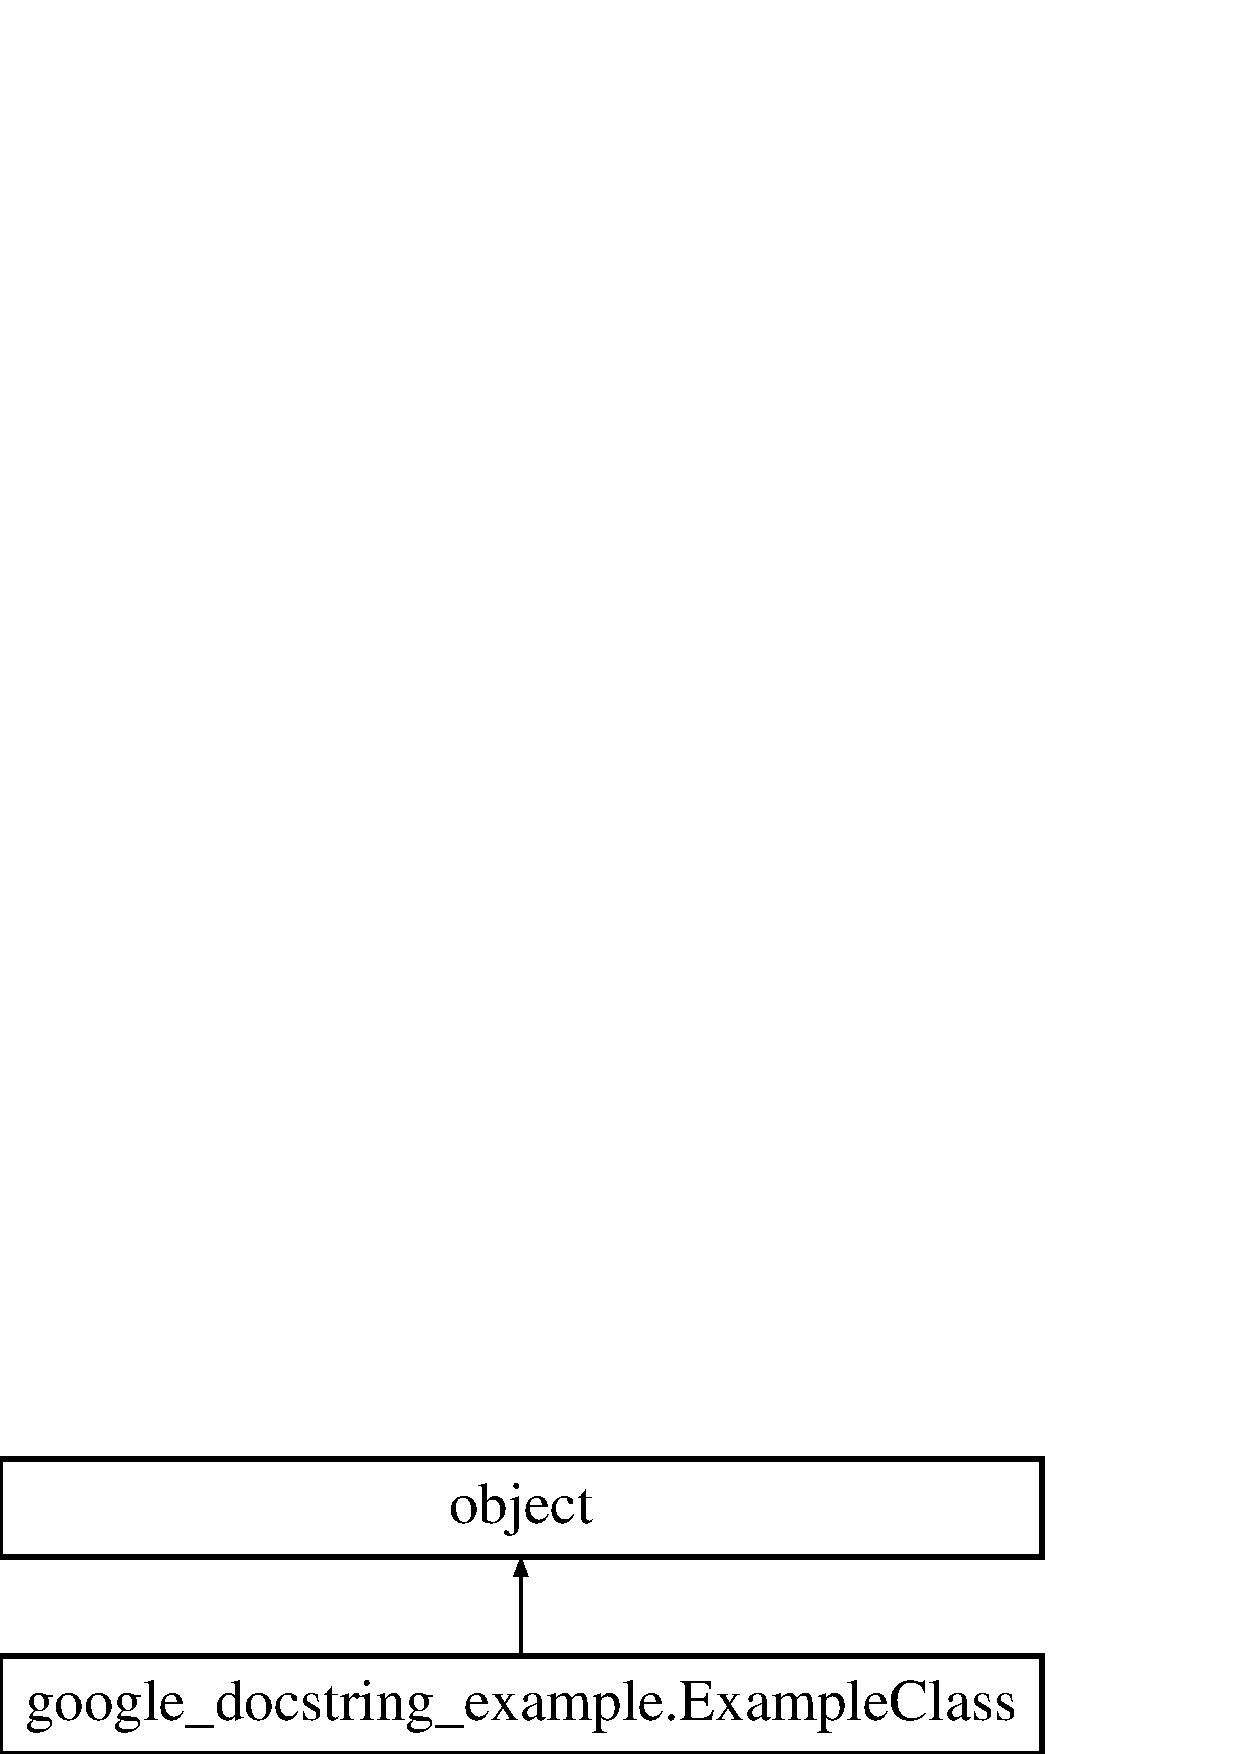
\includegraphics[height=2.000000cm]{classgoogle__docstring__example_1_1ExampleClass}
\end{center}
\end{figure}
\subsection*{Public Member Functions}
\begin{DoxyCompactItemize}
\item 
def \hyperlink{classgoogle__docstring__example_1_1ExampleClass_a6fde9c776090979b1bdd97ab905cdebf}{\-\_\-\-\_\-init\-\_\-\-\_\-}
\item 
def \hyperlink{classgoogle__docstring__example_1_1ExampleClass_aa1788edcf36597ca202110e4f1e540a1}{example\-\_\-method}
\item 
def \hyperlink{classgoogle__docstring__example_1_1ExampleClass_a1d452ef6f6945b82952f17b1b2948ddc}{\-\_\-\-\_\-special\-\_\-\-\_\-}
\item 
\hypertarget{classgoogle__docstring__example_1_1ExampleClass_a32c333c513d78d5b1af25b9d2f0494d2}{def {\bfseries \-\_\-\-\_\-special\-\_\-without\-\_\-docstring\-\_\-\-\_\-}}\label{classgoogle__docstring__example_1_1ExampleClass_a32c333c513d78d5b1af25b9d2f0494d2}

\end{DoxyCompactItemize}
\subsection*{Public Attributes}
\begin{DoxyCompactItemize}
\item 
\hypertarget{classgoogle__docstring__example_1_1ExampleClass_a6fa2ed2716c1ae7ec406eeb02329d652}{{\bfseries attr1}}\label{classgoogle__docstring__example_1_1ExampleClass_a6fa2ed2716c1ae7ec406eeb02329d652}

\item 
\hypertarget{classgoogle__docstring__example_1_1ExampleClass_aeace93f22e79d4dbb60e1bac15b149fa}{{\bfseries attr2}}\label{classgoogle__docstring__example_1_1ExampleClass_aeace93f22e79d4dbb60e1bac15b149fa}

\item 
\hypertarget{classgoogle__docstring__example_1_1ExampleClass_a0425bdc97a8a3e22a92aeb40aa9f9416}{{\bfseries attr3}}\label{classgoogle__docstring__example_1_1ExampleClass_a0425bdc97a8a3e22a92aeb40aa9f9416}

\end{DoxyCompactItemize}


\subsection{Detailed Description}
\begin{DoxyVerb}The summary line for a class docstring should fit on one line.

If the class has public attributes, they should be documented here
in an ``Attributes`` section and follow the same formatting as a
function's ``Args`` section.

Attributes:
  attr1 (str): Description of `attr1`.
  attr2 (list of str): Description of `attr2`.
  attr3 (int): Description of `attr3`.\end{DoxyVerb}
 

\subsection{Constructor \& Destructor Documentation}
\hypertarget{classgoogle__docstring__example_1_1ExampleClass_a6fde9c776090979b1bdd97ab905cdebf}{\index{google\-\_\-docstring\-\_\-example\-::\-Example\-Class@{google\-\_\-docstring\-\_\-example\-::\-Example\-Class}!\-\_\-\-\_\-init\-\_\-\-\_\-@{\-\_\-\-\_\-init\-\_\-\-\_\-}}
\index{\-\_\-\-\_\-init\-\_\-\-\_\-@{\-\_\-\-\_\-init\-\_\-\-\_\-}!google_docstring_example::ExampleClass@{google\-\_\-docstring\-\_\-example\-::\-Example\-Class}}
\subsubsection[{\-\_\-\-\_\-init\-\_\-\-\_\-}]{\setlength{\rightskip}{0pt plus 5cm}def google\-\_\-docstring\-\_\-example.\-Example\-Class.\-\_\-\-\_\-init\-\_\-\-\_\- (
\begin{DoxyParamCaption}
\item[{}]{self, }
\item[{}]{param1, }
\item[{}]{param2, }
\item[{}]{param3 = {\ttfamily 0}}
\end{DoxyParamCaption}
)}}\label{classgoogle__docstring__example_1_1ExampleClass_a6fde9c776090979b1bdd97ab905cdebf}
\begin{DoxyVerb}Example of docstring on the __init__ method.

The __init__ method may be documented in either the class level
docstring, or as a docstring on the __init__ method itself.

Either form is acceptable, but the two should not be mixed. Choose one
convention to document the __init__ method and be consistent with it.

Note:
  Do not include the `self` parameter in the ``Args`` section.

Args:
  param1 (str): Description of `param1`.
  param2 (list of str): Description of `param2`. Multiple
    lines are supported.
  param3 (int, optional): Description of `param3`, defaults to 0.\end{DoxyVerb}
 

References google\-\_\-docstring\-\_\-example.\-Example\-Class.\-attr1, google\-\_\-docstring\-\_\-example.\-Example\-Class.\-attr2, and google\-\_\-docstring\-\_\-example.\-Example\-Class.\-attr3.


\begin{DoxyCode}
150 
151     \textcolor{keyword}{def }\hyperlink{classgoogle__docstring__example_1_1ExampleClass_a6fde9c776090979b1bdd97ab905cdebf}{\_\_init\_\_}(self, param1, param2, param3=0):
152         \textcolor{stringliteral}{"""Example of docstring on the \_\_init\_\_ method.}
153 \textcolor{stringliteral}{}
154 \textcolor{stringliteral}{        The \_\_init\_\_ method may be documented in either the class level}
155 \textcolor{stringliteral}{        docstring, or as a docstring on the \_\_init\_\_ method itself.}
156 \textcolor{stringliteral}{}
157 \textcolor{stringliteral}{        Either form is acceptable, but the two should not be mixed. Choose one}
158 \textcolor{stringliteral}{        convention to document the \_\_init\_\_ method and be consistent with it.}
159 \textcolor{stringliteral}{}
160 \textcolor{stringliteral}{        Note:}
161 \textcolor{stringliteral}{          Do not include the `self` parameter in the ``Args`` section.}
162 \textcolor{stringliteral}{}
163 \textcolor{stringliteral}{        Args:}
164 \textcolor{stringliteral}{          param1 (str): Description of `param1`.}
165 \textcolor{stringliteral}{          param2 (list of str): Description of `param2`. Multiple}
166 \textcolor{stringliteral}{            lines are supported.}
167 \textcolor{stringliteral}{          param3 (int, optional): Description of `param3`, defaults to 0.}
168 \textcolor{stringliteral}{}
169 \textcolor{stringliteral}{        """}
170         self.\hyperlink{classgoogle__docstring__example_1_1ExampleClass_a6fa2ed2716c1ae7ec406eeb02329d652}{attr1} = param1
171         self.\hyperlink{classgoogle__docstring__example_1_1ExampleClass_aeace93f22e79d4dbb60e1bac15b149fa}{attr2} = param2
172         self.\hyperlink{classgoogle__docstring__example_1_1ExampleClass_a0425bdc97a8a3e22a92aeb40aa9f9416}{attr3} = param3

\end{DoxyCode}


\subsection{Member Function Documentation}
\hypertarget{classgoogle__docstring__example_1_1ExampleClass_a1d452ef6f6945b82952f17b1b2948ddc}{\index{google\-\_\-docstring\-\_\-example\-::\-Example\-Class@{google\-\_\-docstring\-\_\-example\-::\-Example\-Class}!\-\_\-\-\_\-special\-\_\-\-\_\-@{\-\_\-\-\_\-special\-\_\-\-\_\-}}
\index{\-\_\-\-\_\-special\-\_\-\-\_\-@{\-\_\-\-\_\-special\-\_\-\-\_\-}!google_docstring_example::ExampleClass@{google\-\_\-docstring\-\_\-example\-::\-Example\-Class}}
\subsubsection[{\-\_\-\-\_\-special\-\_\-\-\_\-}]{\setlength{\rightskip}{0pt plus 5cm}def google\-\_\-docstring\-\_\-example.\-Example\-Class.\-\_\-\-\_\-special\-\_\-\-\_\- (
\begin{DoxyParamCaption}
\item[{}]{self}
\end{DoxyParamCaption}
)}}\label{classgoogle__docstring__example_1_1ExampleClass_a1d452ef6f6945b82952f17b1b2948ddc}
\begin{DoxyVerb}By default special members with docstrings are included.

Special members are any methods or attributes that start with and
end with a double underscore. Any special member with a docstring
will be included in the output.

This behavior can be disabled by changing the following setting in
Sphinx's conf.py::

    napoleon_include_special_with_doc = False\end{DoxyVerb}
 
\begin{DoxyCode}
189 
190     \textcolor{keyword}{def }\hyperlink{classgoogle__docstring__example_1_1ExampleClass_a1d452ef6f6945b82952f17b1b2948ddc}{\_\_special\_\_}(self):
191         \textcolor{stringliteral}{"""By default special members with docstrings are included.}
192 \textcolor{stringliteral}{}
193 \textcolor{stringliteral}{        Special members are any methods or attributes that start with and}
194 \textcolor{stringliteral}{        end with a double underscore. Any special member with a docstring}
195 \textcolor{stringliteral}{        will be included in the output.}
196 \textcolor{stringliteral}{}
197 \textcolor{stringliteral}{        This behavior can be disabled by changing the following setting in}
198 \textcolor{stringliteral}{        Sphinx's conf.py::}
199 \textcolor{stringliteral}{}
200 \textcolor{stringliteral}{            napoleon\_include\_special\_with\_doc = False}
201 \textcolor{stringliteral}{}
202 \textcolor{stringliteral}{        """}
203         \textcolor{keywordflow}{pass}

\end{DoxyCode}
\hypertarget{classgoogle__docstring__example_1_1ExampleClass_aa1788edcf36597ca202110e4f1e540a1}{\index{google\-\_\-docstring\-\_\-example\-::\-Example\-Class@{google\-\_\-docstring\-\_\-example\-::\-Example\-Class}!example\-\_\-method@{example\-\_\-method}}
\index{example\-\_\-method@{example\-\_\-method}!google_docstring_example::ExampleClass@{google\-\_\-docstring\-\_\-example\-::\-Example\-Class}}
\subsubsection[{example\-\_\-method}]{\setlength{\rightskip}{0pt plus 5cm}def google\-\_\-docstring\-\_\-example.\-Example\-Class.\-example\-\_\-method (
\begin{DoxyParamCaption}
\item[{}]{self, }
\item[{}]{param1, }
\item[{}]{param2}
\end{DoxyParamCaption}
)}}\label{classgoogle__docstring__example_1_1ExampleClass_aa1788edcf36597ca202110e4f1e540a1}
\begin{DoxyVerb}Class methods are similar to regular functions.

Note:
  Do not include the `self` parameter in the ``Args`` section.

Args:
  param1: The first parameter.
  param2: The second parameter.

Returns:
  True if successful, False otherwise.\end{DoxyVerb}
 
\begin{DoxyCode}
173 
174     \textcolor{keyword}{def }\hyperlink{classgoogle__docstring__example_1_1ExampleClass_aa1788edcf36597ca202110e4f1e540a1}{example\_method}(self, param1, param2):
175         \textcolor{stringliteral}{"""Class methods are similar to regular functions.}
176 \textcolor{stringliteral}{}
177 \textcolor{stringliteral}{        Note:}
178 \textcolor{stringliteral}{          Do not include the `self` parameter in the ``Args`` section.}
179 \textcolor{stringliteral}{}
180 \textcolor{stringliteral}{        Args:}
181 \textcolor{stringliteral}{          param1: The first parameter.}
182 \textcolor{stringliteral}{          param2: The second parameter.}
183 \textcolor{stringliteral}{}
184 \textcolor{stringliteral}{        Returns:}
185 \textcolor{stringliteral}{          True if successful, False otherwise.}
186 \textcolor{stringliteral}{}
187 \textcolor{stringliteral}{        """}
188         \textcolor{keywordflow}{return} \textcolor{keyword}{True}

\end{DoxyCode}


The documentation for this class was generated from the following file\-:\begin{DoxyCompactItemize}
\item 
docs/style\-\_\-standards/google\-\_\-docstring\-\_\-example.\-py\end{DoxyCompactItemize}

\hypertarget{classgoogle__docstring__example_1_1ExampleError}{\section{google\-\_\-docstring\-\_\-example.\-Example\-Error Class Reference}
\label{classgoogle__docstring__example_1_1ExampleError}\index{google\-\_\-docstring\-\_\-example.\-Example\-Error@{google\-\_\-docstring\-\_\-example.\-Example\-Error}}
}
Inheritance diagram for google\-\_\-docstring\-\_\-example.\-Example\-Error\-:\begin{figure}[H]
\begin{center}
\leavevmode
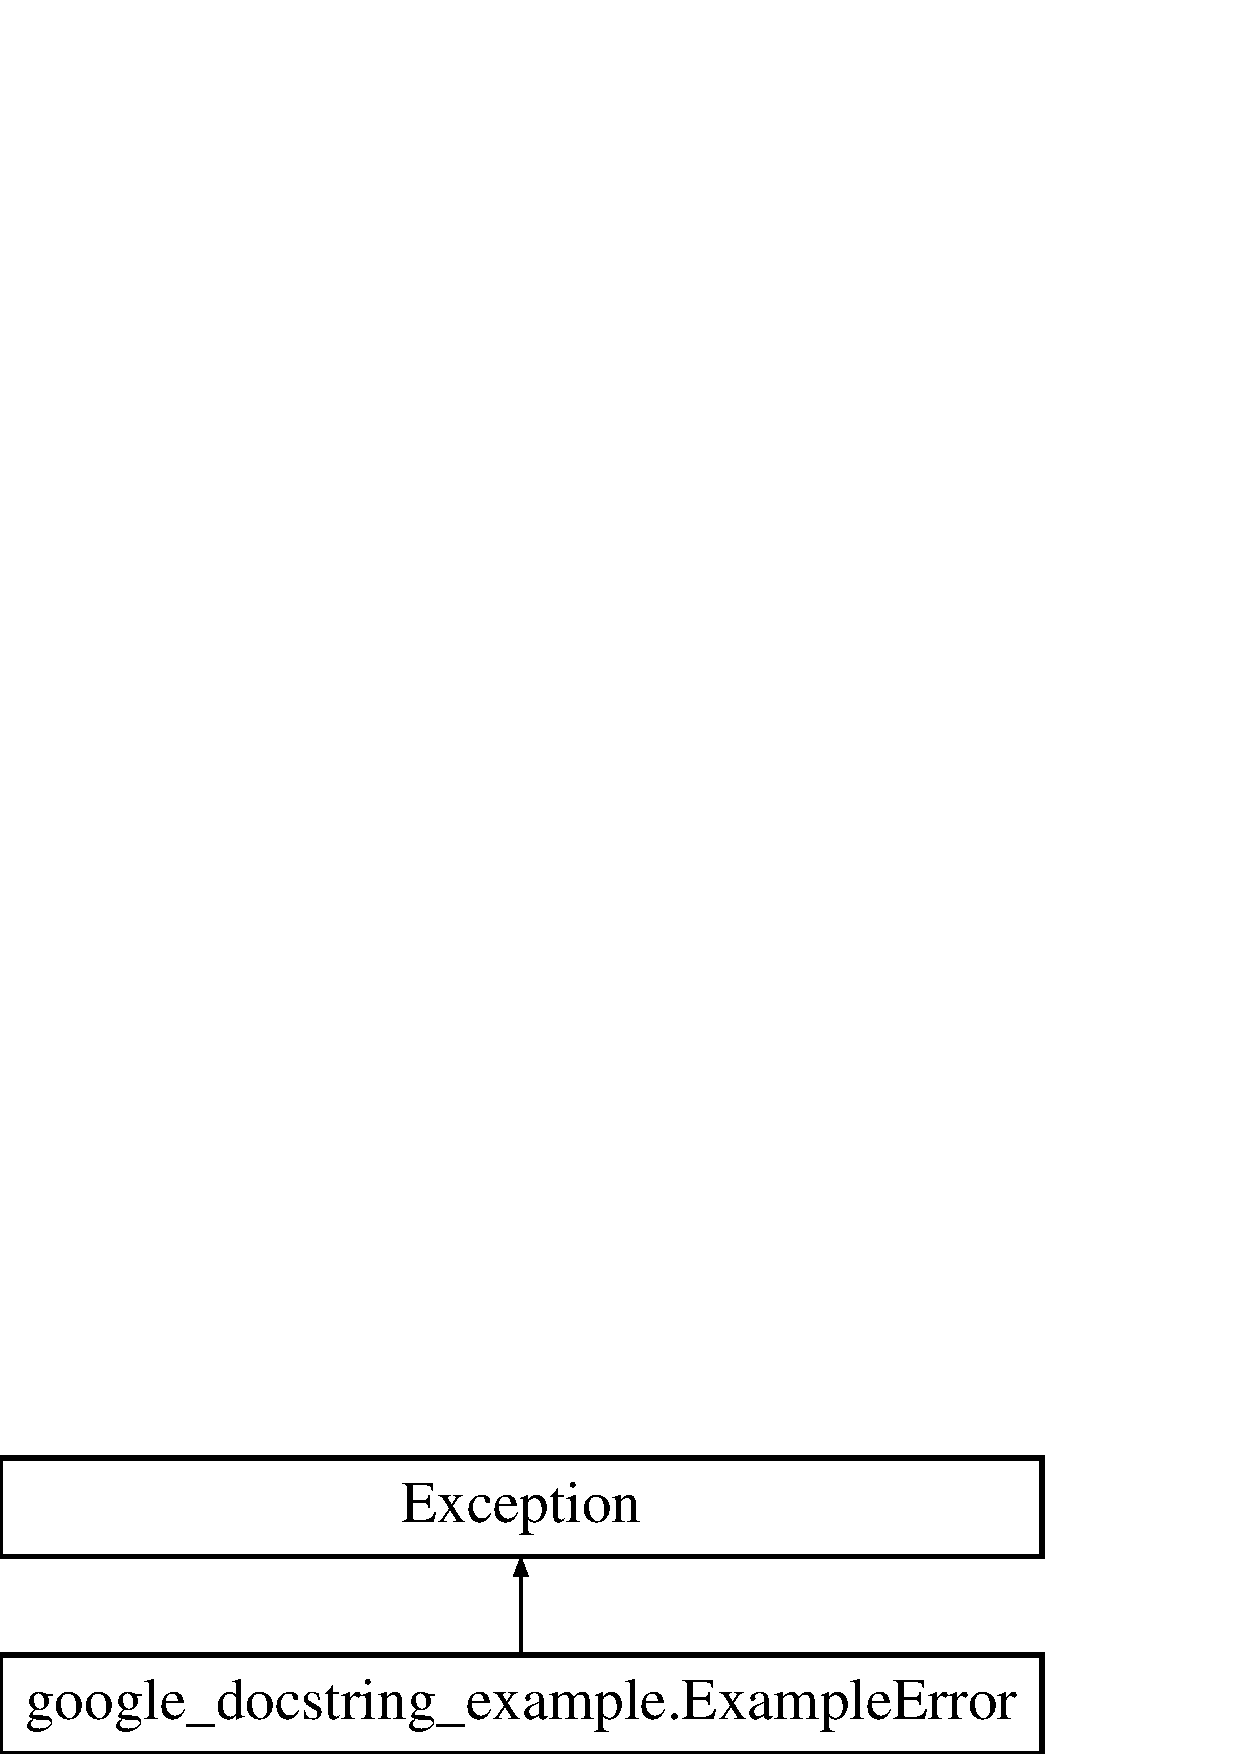
\includegraphics[height=2.000000cm]{classgoogle__docstring__example_1_1ExampleError}
\end{center}
\end{figure}
\subsection*{Public Member Functions}
\begin{DoxyCompactItemize}
\item 
\hypertarget{classgoogle__docstring__example_1_1ExampleError_a7f82075efd3e0aef9e7db900ea7dd961}{def {\bfseries \-\_\-\-\_\-init\-\_\-\-\_\-}}\label{classgoogle__docstring__example_1_1ExampleError_a7f82075efd3e0aef9e7db900ea7dd961}

\end{DoxyCompactItemize}
\subsection*{Public Attributes}
\begin{DoxyCompactItemize}
\item 
\hypertarget{classgoogle__docstring__example_1_1ExampleError_aa84a97ad68bbe5f5e5b96598396a3ae0}{{\bfseries msg}}\label{classgoogle__docstring__example_1_1ExampleError_aa84a97ad68bbe5f5e5b96598396a3ae0}

\item 
\hypertarget{classgoogle__docstring__example_1_1ExampleError_a749126a25024f84564afcba15a8b7b0f}{{\bfseries code}}\label{classgoogle__docstring__example_1_1ExampleError_a749126a25024f84564afcba15a8b7b0f}

\end{DoxyCompactItemize}


\subsection{Detailed Description}
\begin{DoxyVerb}Exceptions are documented in the same way as classes.

The __init__ method may be documented in either the class level
docstring, or as a docstring on the __init__ method itself.

Either form is acceptable, but the two should not be mixed. Choose one
convention to document the __init__ method and be consistent with it.

Note:
  Do not include the `self` parameter in the ``Args`` section.

Args:
  msg (str): Human readable string describing the exception.
  code (int, optional): Error code, defaults to 2.

Attributes:
  msg (str): Human readable string describing the exception.
  code (int): Exception error code.\end{DoxyVerb}
 

The documentation for this class was generated from the following file\-:\begin{DoxyCompactItemize}
\item 
docs/style\-\_\-standards/google\-\_\-docstring\-\_\-example.\-py\end{DoxyCompactItemize}

\hypertarget{classtests_1_1utils_1_1extension__manager__tests_1_1ExtensionLibraries}{\section{tests.\+utils.\+extension\+\_\+manager\+\_\+tests.\+Extension\+Libraries Class Reference}
\label{classtests_1_1utils_1_1extension__manager__tests_1_1ExtensionLibraries}\index{tests.\+utils.\+extension\+\_\+manager\+\_\+tests.\+Extension\+Libraries@{tests.\+utils.\+extension\+\_\+manager\+\_\+tests.\+Extension\+Libraries}}
}
Inheritance diagram for tests.\+utils.\+extension\+\_\+manager\+\_\+tests.\+Extension\+Libraries\+:\begin{figure}[H]
\begin{center}
\leavevmode
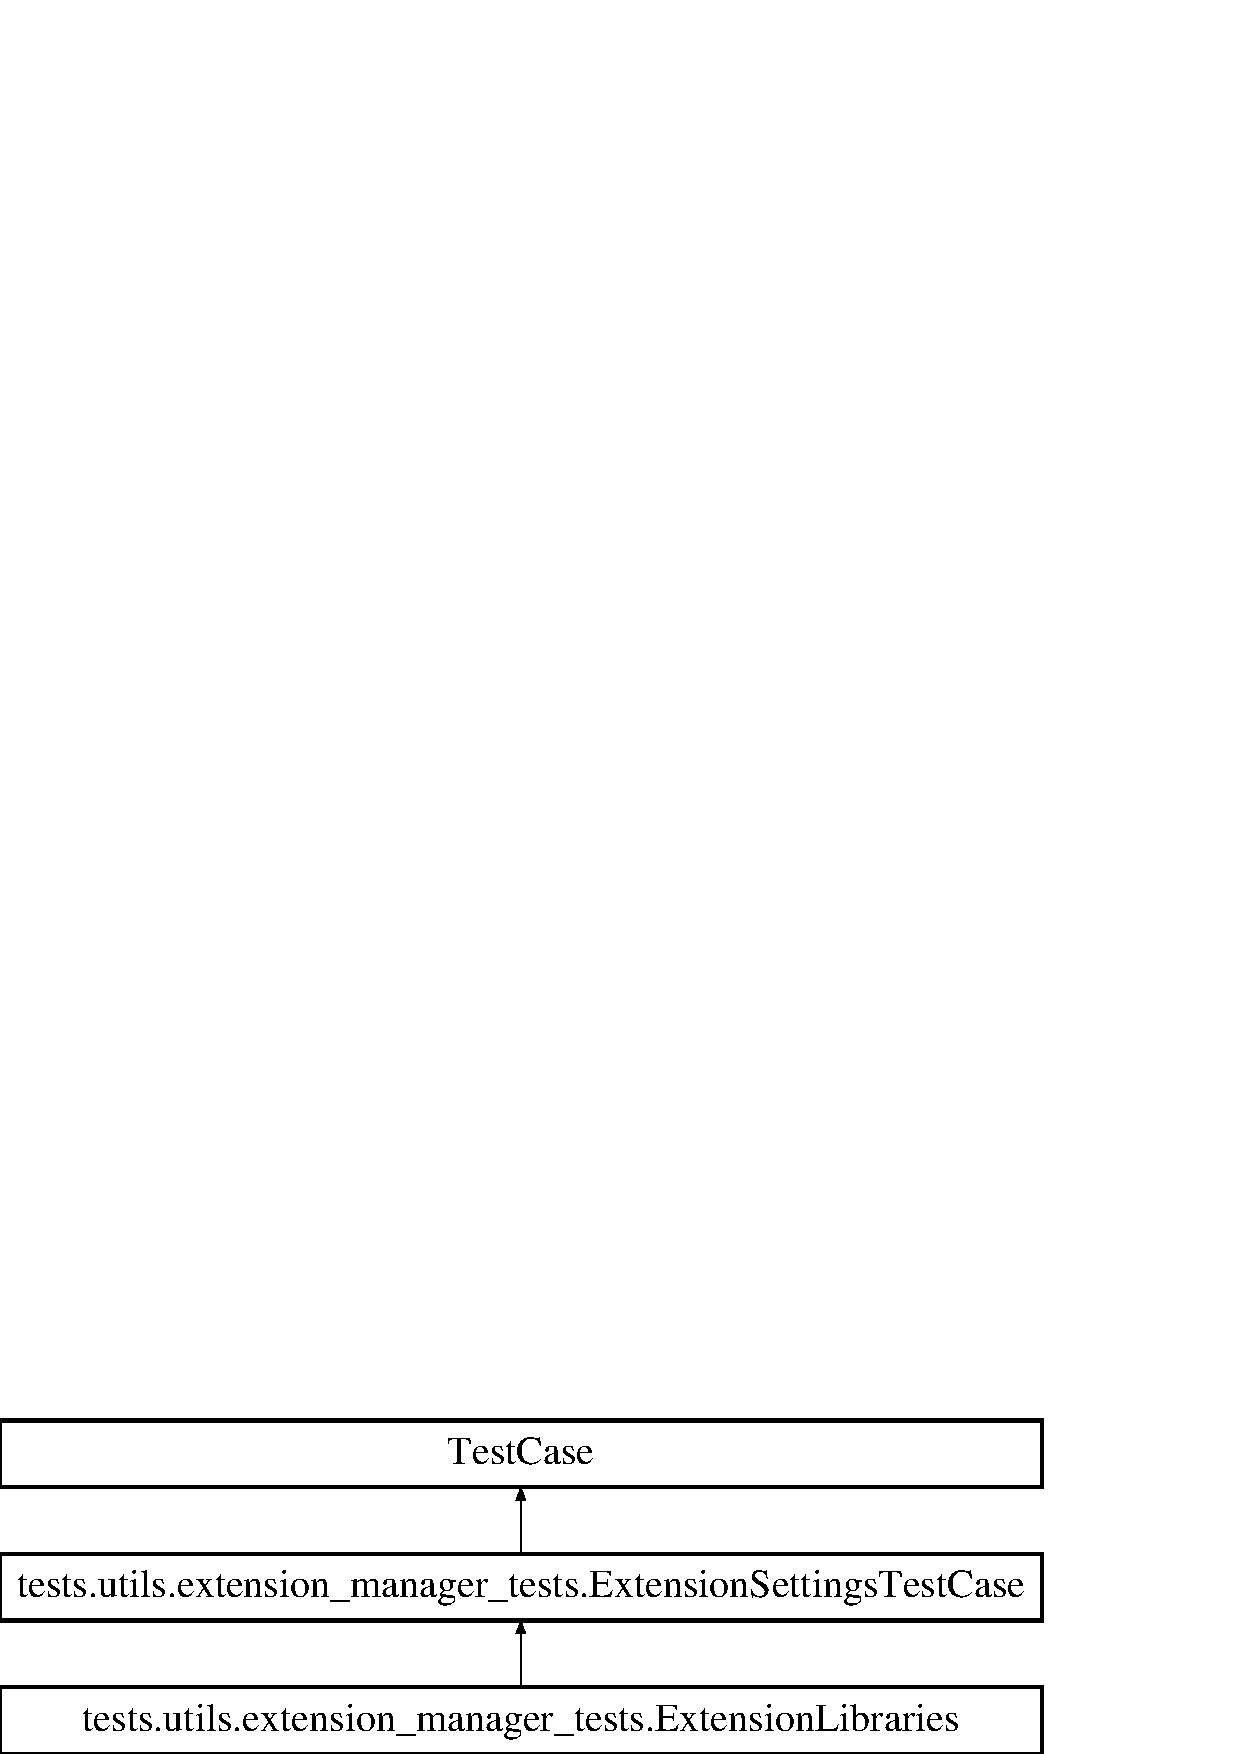
\includegraphics[height=3.000000cm]{classtests_1_1utils_1_1extension__manager__tests_1_1ExtensionLibraries}
\end{center}
\end{figure}
\subsection*{Public Member Functions}
\begin{DoxyCompactItemize}
\item 
def \hyperlink{classtests_1_1utils_1_1extension__manager__tests_1_1ExtensionLibraries_af3f2d4803bef48691d5508edd8095c96}{test\+\_\+init\+\_\+libraries}
\item 
def \hyperlink{classtests_1_1utils_1_1extension__manager__tests_1_1ExtensionLibraries_a73dd723752e59cf02a86230335645e52}{test\+\_\+install\+\_\+loaded}
\item 
\hypertarget{classtests_1_1utils_1_1extension__manager__tests_1_1ExtensionLibraries_a23c733ce54eb18f32009b57923399bc2}{def {\bfseries test\+\_\+get\+\_\+extension\+\_\+from\+\_\+property}}\label{classtests_1_1utils_1_1extension__manager__tests_1_1ExtensionLibraries_a23c733ce54eb18f32009b57923399bc2}

\item 
\hypertarget{classtests_1_1utils_1_1extension__manager__tests_1_1ExtensionLibraries_a382720c0522135d0f08ff4f7c29dc68a}{def {\bfseries test\+\_\+get\+\_\+property}}\label{classtests_1_1utils_1_1extension__manager__tests_1_1ExtensionLibraries_a382720c0522135d0f08ff4f7c29dc68a}

\item 
\hypertarget{classtests_1_1utils_1_1extension__manager__tests_1_1ExtensionLibraries_a31a4a900c6de3db5920d9412c14c83e8}{def {\bfseries test\+\_\+load\+\_\+user\+\_\+interface}}\label{classtests_1_1utils_1_1extension__manager__tests_1_1ExtensionLibraries_a31a4a900c6de3db5920d9412c14c83e8}

\item 
\hypertarget{classtests_1_1utils_1_1extension__manager__tests_1_1ExtensionLibraries_a74dc43c98b82c21c36b95dc297927975}{def {\bfseries test\+\_\+get\+\_\+config}}\label{classtests_1_1utils_1_1extension__manager__tests_1_1ExtensionLibraries_a74dc43c98b82c21c36b95dc297927975}

\item 
\hypertarget{classtests_1_1utils_1_1extension__manager__tests_1_1ExtensionLibraries_afd57bd3b7f63f9362d638f7665fd710f}{def {\bfseries test\+\_\+reset\+\_\+settings\+\_\+group}}\label{classtests_1_1utils_1_1extension__manager__tests_1_1ExtensionLibraries_afd57bd3b7f63f9362d638f7665fd710f}

\item 
\hypertarget{classtests_1_1utils_1_1extension__manager__tests_1_1ExtensionLibraries_a895b31bae8dc08628b94ad459451f8e8}{def {\bfseries test\+\_\+remove\+\_\+extension\+\_\+settings}}\label{classtests_1_1utils_1_1extension__manager__tests_1_1ExtensionLibraries_a895b31bae8dc08628b94ad459451f8e8}

\item 
\hypertarget{classtests_1_1utils_1_1extension__manager__tests_1_1ExtensionLibraries_accef069e9ae24484e7a873b3f94aea48}{def {\bfseries test\+\_\+save\+\_\+settings}}\label{classtests_1_1utils_1_1extension__manager__tests_1_1ExtensionLibraries_accef069e9ae24484e7a873b3f94aea48}

\end{DoxyCompactItemize}
\subsection*{Additional Inherited Members}


\subsection{Member Function Documentation}
\hypertarget{classtests_1_1utils_1_1extension__manager__tests_1_1ExtensionLibraries_af3f2d4803bef48691d5508edd8095c96}{\index{tests\+::utils\+::extension\+\_\+manager\+\_\+tests\+::\+Extension\+Libraries@{tests\+::utils\+::extension\+\_\+manager\+\_\+tests\+::\+Extension\+Libraries}!test\+\_\+init\+\_\+libraries@{test\+\_\+init\+\_\+libraries}}
\index{test\+\_\+init\+\_\+libraries@{test\+\_\+init\+\_\+libraries}!tests\+::utils\+::extension\+\_\+manager\+\_\+tests\+::\+Extension\+Libraries@{tests\+::utils\+::extension\+\_\+manager\+\_\+tests\+::\+Extension\+Libraries}}
\subsubsection[{test\+\_\+init\+\_\+libraries}]{\setlength{\rightskip}{0pt plus 5cm}def tests.\+utils.\+extension\+\_\+manager\+\_\+tests.\+Extension\+Libraries.\+test\+\_\+init\+\_\+libraries (
\begin{DoxyParamCaption}
\item[{}]{self}
\end{DoxyParamCaption}
)}}\label{classtests_1_1utils_1_1extension__manager__tests_1_1ExtensionLibraries_af3f2d4803bef48691d5508edd8095c96}
\begin{DoxyVerb}Tests that the library are created when provided and fail gracefully when not. \end{DoxyVerb}
 
\begin{DoxyCode}
169 
170     \textcolor{keyword}{def }\hyperlink{classtests_1_1utils_1_1extension__manager__tests_1_1ExtensionLibraries_af3f2d4803bef48691d5508edd8095c96}{test\_init\_libraries}(self):
171         \textcolor{stringliteral}{"""Tests that the library are created when provided and fail gracefully when not. """}
172 
173         \textcolor{comment}{#init libraries from library defaults}
174         self.ext\_mgr.set\_library\_defaults()
175         user\_dir = self.ext\_mgr.libraries[\textcolor{stringliteral}{'user'}]
176         \textcolor{comment}{#Set global path to be a temporary path because it pulls the application path, which is pythons
       /usr/local/bin path which we don't have permissions for.}
177         self.ext\_mgr.libraries[\textcolor{stringliteral}{'global'}] = os.path.abspath(\textcolor{stringliteral}{"tests/temp/"})
178         global\_dir = self.ext\_mgr.libraries[\textcolor{stringliteral}{'global'}]
179         self.ext\_mgr.init\_libraries()
180         self.assertTrue(os.path.isdir(os.path.abspath(user\_dir)))
181         self.assertTrue(os.path.isdir(os.path.abspath(global\_dir)))
182         \textcolor{comment}{#assert that init libraries works with non-default paths.}
183         
184         self.ext\_mgr.libraries[\textcolor{stringliteral}{'user'}] = os.path.abspath(\textcolor{stringliteral}{"tests/temp/oneLevel/"})
185         self.ext\_mgr.libraries[\textcolor{stringliteral}{'global'}] = os.path.abspath(\textcolor{stringliteral}{"tests/temp/oneLevel/twoLevel/"})
186         self.ext\_mgr.init\_libraries()
187         self.assertTrue(os.path.isdir(os.path.abspath(\textcolor{stringliteral}{"tests/temp/oneLevel/twoLevel/"})))
188         self.assertTrue(os.path.isdir(os.path.abspath(\textcolor{stringliteral}{"tests/temp/oneLevel/"})))

\end{DoxyCode}
\hypertarget{classtests_1_1utils_1_1extension__manager__tests_1_1ExtensionLibraries_a73dd723752e59cf02a86230335645e52}{\index{tests\+::utils\+::extension\+\_\+manager\+\_\+tests\+::\+Extension\+Libraries@{tests\+::utils\+::extension\+\_\+manager\+\_\+tests\+::\+Extension\+Libraries}!test\+\_\+install\+\_\+loaded@{test\+\_\+install\+\_\+loaded}}
\index{test\+\_\+install\+\_\+loaded@{test\+\_\+install\+\_\+loaded}!tests\+::utils\+::extension\+\_\+manager\+\_\+tests\+::\+Extension\+Libraries@{tests\+::utils\+::extension\+\_\+manager\+\_\+tests\+::\+Extension\+Libraries}}
\subsubsection[{test\+\_\+install\+\_\+loaded}]{\setlength{\rightskip}{0pt plus 5cm}def tests.\+utils.\+extension\+\_\+manager\+\_\+tests.\+Extension\+Libraries.\+test\+\_\+install\+\_\+loaded (
\begin{DoxyParamCaption}
\item[{}]{self}
\end{DoxyParamCaption}
)}}\label{classtests_1_1utils_1_1extension__manager__tests_1_1ExtensionLibraries_a73dd723752e59cf02a86230335645e52}
\begin{DoxyVerb}Tests that all loaded, and currently uninstalled, libraries are installed\end{DoxyVerb}
 
\begin{DoxyCode}
189 
190     \textcolor{keyword}{def }\hyperlink{classtests_1_1utils_1_1extension__manager__tests_1_1ExtensionLibraries_a73dd723752e59cf02a86230335645e52}{test\_install\_loaded}(self):
191         \textcolor{stringliteral}{""" Tests that all loaded, and currently uninstalled, libraries are installed"""}
192         \textcolor{comment}{#setup directory with extension}
193         self.ext\_mgr.libraries[\textcolor{stringliteral}{'user'}] = os.path.abspath(\textcolor{stringliteral}{"tests/mock/extensions/"})
194         \textcolor{comment}{#setup empty directory}
195         self.ext\_mgr.libraries[\textcolor{stringliteral}{'global'}] = os.path.abspath(\textcolor{stringliteral}{"tests/temp/global/"})
196         \textcolor{comment}{#setup paths and configs}
197         self.ext\_mgr.init\_libraries()
198         self.ext\_mgr.init\_extension\_config(\textcolor{stringliteral}{"user"})
199         self.ext\_mgr.init\_extension\_config(\textcolor{stringliteral}{"global"})
200         \textcolor{comment}{#Global is empty, so make sure it is not filled.}
201         with self.assertRaises(KeyError):
202             self.ext\_mgr.extensions[\textcolor{stringliteral}{'global'}].has\_configs()
203         \textcolor{comment}{#run function}
204         user\_installed = self.ext\_mgr.install\_loaded()
205         self.assertEqual(user\_installed, [\textcolor{stringliteral}{"unit\_test\_mock"}])
206 
207         \textcolor{comment}{#Test that the mock extension was loaded}
208         self.assertTrue(self.ext\_mgr.check\_installed(\textcolor{stringliteral}{"unit\_test\_mock"}))
209         \textcolor{comment}{#Test that ONLY the mock extension was loaded and in the user section}
210         one\_item\_only = self.ext\_mgr.get\_installed()
211         self.assertEqual(len(one\_item\_only), 1)
212         self.assertIn(\textcolor{stringliteral}{"unit\_test\_mock"}, one\_item\_only)
213         self.assertEqual(one\_item\_only[\textcolor{stringliteral}{'unit\_test\_mock'}], \textcolor{stringliteral}{'user'})
214         \textcolor{comment}{#Test that the config\_manager was "initialized".}
215         initialized = self.ext\_mgr.get\_extension\_from\_property(\textcolor{stringliteral}{"initialized"}, \textcolor{keyword}{True})
216         self.assertIn(\textcolor{stringliteral}{"unit\_test\_mock"}, initialized)

\end{DoxyCode}


The documentation for this class was generated from the following file\+:\begin{DoxyCompactItemize}
\item 
tests/utils/extension\+\_\+manager\+\_\+tests.\+py\end{DoxyCompactItemize}

\hypertarget{classcommotion__client_1_1utils_1_1extension__manager_1_1ExtensionManager}{\section{commotion\+\_\+client.\+utils.\+extension\+\_\+manager.\+Extension\+Manager Class Reference}
\label{classcommotion__client_1_1utils_1_1extension__manager_1_1ExtensionManager}\index{commotion\+\_\+client.\+utils.\+extension\+\_\+manager.\+Extension\+Manager@{commotion\+\_\+client.\+utils.\+extension\+\_\+manager.\+Extension\+Manager}}
}
Inheritance diagram for commotion\+\_\+client.\+utils.\+extension\+\_\+manager.\+Extension\+Manager\+:\begin{figure}[H]
\begin{center}
\leavevmode
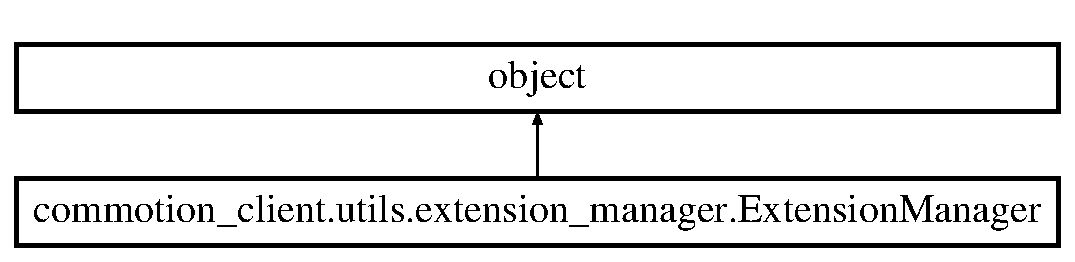
\includegraphics[height=2.000000cm]{classcommotion__client_1_1utils_1_1extension__manager_1_1ExtensionManager}
\end{center}
\end{figure}
\subsection*{Public Member Functions}
\begin{DoxyCompactItemize}
\item 
\hypertarget{classcommotion__client_1_1utils_1_1extension__manager_1_1ExtensionManager_a98ed5baeb8363089a665d7a4fbcc6198}{def {\bfseries \+\_\+\+\_\+init\+\_\+\+\_\+}}\label{classcommotion__client_1_1utils_1_1extension__manager_1_1ExtensionManager_a98ed5baeb8363089a665d7a4fbcc6198}

\item 
def \hyperlink{classcommotion__client_1_1utils_1_1extension__manager_1_1ExtensionManager_a25c38ac92dceebe57891ce0ed422505e}{get\+\_\+user\+\_\+settings}
\item 
def \hyperlink{classcommotion__client_1_1utils_1_1extension__manager_1_1ExtensionManager_ae90e7bfde555094ce23154a21baafd02}{reset\+\_\+settings\+\_\+group}
\item 
def \hyperlink{classcommotion__client_1_1utils_1_1extension__manager_1_1ExtensionManager_a5a94323a3528a6af3bf009eb302fa729}{init\+\_\+extension\+\_\+libraries}
\item 
def \hyperlink{classcommotion__client_1_1utils_1_1extension__manager_1_1ExtensionManager_ab2a55f25d0f1dbce2924c28513fac830}{set\+\_\+library\+\_\+defaults}
\item 
def \hyperlink{classcommotion__client_1_1utils_1_1extension__manager_1_1ExtensionManager_a2edb9c39e0b8e5143c245089170182a3}{init\+\_\+libraries}
\item 
def \hyperlink{classcommotion__client_1_1utils_1_1extension__manager_1_1ExtensionManager_ae751a1b407e33af012d41ec44f2ce717}{init\+\_\+extension\+\_\+config}
\item 
def \hyperlink{classcommotion__client_1_1utils_1_1extension__manager_1_1ExtensionManager_a549fdfd52d8e355e4bac34907ef74e2a}{check\+\_\+installed}
\item 
def \hyperlink{classcommotion__client_1_1utils_1_1extension__manager_1_1ExtensionManager_aa2b5054f6495fbc20e556f5713550d01}{get\+\_\+installed}
\item 
def \hyperlink{classcommotion__client_1_1utils_1_1extension__manager_1_1ExtensionManager_a98f5f3c261f083885a9b0528dcdafd34}{load\+\_\+core}
\item 
def \hyperlink{classcommotion__client_1_1utils_1_1extension__manager_1_1ExtensionManager_a58bcb83cefe458d4affcb185785694c6}{install\+\_\+loaded}
\item 
def \hyperlink{classcommotion__client_1_1utils_1_1extension__manager_1_1ExtensionManager_ac5a486ac7518727f2fab847f989cdfd9}{get\+\_\+extension\+\_\+from\+\_\+property}
\item 
def \hyperlink{classcommotion__client_1_1utils_1_1extension__manager_1_1ExtensionManager_a91552f94535d729789bcb7da471d90fe}{get\+\_\+property}
\item 
def \hyperlink{classcommotion__client_1_1utils_1_1extension__manager_1_1ExtensionManager_a923e4fe2b6bc682d9ccca7820cf2f3f3}{load\+\_\+user\+\_\+interface}
\item 
def \hyperlink{classcommotion__client_1_1utils_1_1extension__manager_1_1ExtensionManager_a7f811f5c953b4208d9af942c9c173dbf}{get\+\_\+config}
\item 
def \hyperlink{classcommotion__client_1_1utils_1_1extension__manager_1_1ExtensionManager_a6d909da9885ddd0ca5a4b1e548bf2257}{remove\+\_\+extension\+\_\+settings}
\item 
def \hyperlink{classcommotion__client_1_1utils_1_1extension__manager_1_1ExtensionManager_a048d2495f31a2637f67ed1b759f728a4}{save\+\_\+settings}
\end{DoxyCompactItemize}
\subsection*{Public Attributes}
\begin{DoxyCompactItemize}
\item 
\hypertarget{classcommotion__client_1_1utils_1_1extension__manager_1_1ExtensionManager_a01771482a71cd6aef4806253e177cd7a}{{\bfseries log}}\label{classcommotion__client_1_1utils_1_1extension__manager_1_1ExtensionManager_a01771482a71cd6aef4806253e177cd7a}

\item 
\hypertarget{classcommotion__client_1_1utils_1_1extension__manager_1_1ExtensionManager_a2cfd032ca383c3fd6f0f52b99b6dd67c}{{\bfseries translate}}\label{classcommotion__client_1_1utils_1_1extension__manager_1_1ExtensionManager_a2cfd032ca383c3fd6f0f52b99b6dd67c}

\item 
\hypertarget{classcommotion__client_1_1utils_1_1extension__manager_1_1ExtensionManager_ab11d3e09be6db88eb58e432c82d82702}{{\bfseries extensions}}\label{classcommotion__client_1_1utils_1_1extension__manager_1_1ExtensionManager_ab11d3e09be6db88eb58e432c82d82702}

\item 
\hypertarget{classcommotion__client_1_1utils_1_1extension__manager_1_1ExtensionManager_a28e035496b4d544179f934b3c401c0c1}{{\bfseries libraries}}\label{classcommotion__client_1_1utils_1_1extension__manager_1_1ExtensionManager_a28e035496b4d544179f934b3c401c0c1}

\item 
\hypertarget{classcommotion__client_1_1utils_1_1extension__manager_1_1ExtensionManager_a0fa8b2be1171ded73629a01c50472d34}{{\bfseries user\+\_\+settings}}\label{classcommotion__client_1_1utils_1_1extension__manager_1_1ExtensionManager_a0fa8b2be1171ded73629a01c50472d34}

\item 
\hypertarget{classcommotion__client_1_1utils_1_1extension__manager_1_1ExtensionManager_a72f3a3497a4593880a56e3952e674b13}{{\bfseries config\+\_\+keys}}\label{classcommotion__client_1_1utils_1_1extension__manager_1_1ExtensionManager_a72f3a3497a4593880a56e3952e674b13}

\end{DoxyCompactItemize}


\subsection{Member Function Documentation}
\hypertarget{classcommotion__client_1_1utils_1_1extension__manager_1_1ExtensionManager_a549fdfd52d8e355e4bac34907ef74e2a}{\index{commotion\+\_\+client\+::utils\+::extension\+\_\+manager\+::\+Extension\+Manager@{commotion\+\_\+client\+::utils\+::extension\+\_\+manager\+::\+Extension\+Manager}!check\+\_\+installed@{check\+\_\+installed}}
\index{check\+\_\+installed@{check\+\_\+installed}!commotion\+\_\+client\+::utils\+::extension\+\_\+manager\+::\+Extension\+Manager@{commotion\+\_\+client\+::utils\+::extension\+\_\+manager\+::\+Extension\+Manager}}
\subsubsection[{check\+\_\+installed}]{\setlength{\rightskip}{0pt plus 5cm}def commotion\+\_\+client.\+utils.\+extension\+\_\+manager.\+Extension\+Manager.\+check\+\_\+installed (
\begin{DoxyParamCaption}
\item[{}]{self, }
\item[{}]{name = {\ttfamily None}}
\end{DoxyParamCaption}
)}}\label{classcommotion__client_1_1utils_1_1extension__manager_1_1ExtensionManager_a549fdfd52d8e355e4bac34907ef74e2a}
\begin{DoxyVerb}Checks if and extension is installed.
    
Args:
  name (type): Name of a extension to check. If not specified will check if there are any extensions installed.
    
Returns:
  bool: True if named extension is installed, false, if not.
\end{DoxyVerb}
 

References commotion\+\_\+client.\+utils.\+extension\+\_\+manager.\+Extension\+Manager.\+get\+\_\+installed(), commotion\+\_\+client.\+G\+U\+I.\+menu\+\_\+bar.\+Menu\+Bar.\+translate, commotion\+\_\+client.\+extensions.\+config\+\_\+editor.\+main.\+View\+Port.\+translate, commotion\+\_\+client.\+G\+U\+I.\+main\+\_\+window.\+Main\+Window.\+translate, commotion\+\_\+client.\+G\+U\+I.\+toolbar\+\_\+builder.\+Tool\+Bar.\+translate, commotion\+\_\+client.\+G\+U\+I.\+extension\+\_\+toolbar.\+Extension\+Tool\+Bar.\+translate, commotion\+\_\+client.\+G\+U\+I.\+toolbar.\+Tool\+Bar.\+translate, commotion\+\_\+client.\+utils.\+extension\+\_\+manager.\+Extension\+Manager.\+translate, commotion\+\_\+client.\+G\+U\+I.\+extension\+\_\+toolbar.\+Menu\+Item.\+translate, and commotion\+\_\+client.\+commotion\+\_\+client.\+Commotion\+Client\+Application.\+translate.


\begin{DoxyCode}
220 
221     \textcolor{keyword}{def }\hyperlink{classcommotion__client_1_1utils_1_1extension__manager_1_1ExtensionManager_a549fdfd52d8e355e4bac34907ef74e2a}{check\_installed}(self, name=None):
222         \textcolor{stringliteral}{"""Checks if and extension is installed.}
223 \textcolor{stringliteral}{            }
224 \textcolor{stringliteral}{        Args:}
225 \textcolor{stringliteral}{          name (type): Name of a extension to check. If not specified will check if there are any
       extensions installed.}
226 \textcolor{stringliteral}{            }
227 \textcolor{stringliteral}{        Returns:}
228 \textcolor{stringliteral}{          bool: True if named extension is installed, false, if not.}
229 \textcolor{stringliteral}{        """}
230         installed\_extensions = list(self.\hyperlink{classcommotion__client_1_1utils_1_1extension__manager_1_1ExtensionManager_aa2b5054f6495fbc20e556f5713550d01}{get\_installed}().keys())
231         \textcolor{keywordflow}{if} name \textcolor{keywordflow}{and} name \textcolor{keywordflow}{in} installed\_extensions:
232             self.log.debug(self.\hyperlink{classcommotion__client_1_1utils_1_1extension__manager_1_1ExtensionManager_a2cfd032ca383c3fd6f0f52b99b6dd67c}{translate}(\textcolor{stringliteral}{"logs"}, \textcolor{stringliteral}{"Extension \{0\} found in installed extensions."}.
      format(name)))
233             \textcolor{keywordflow}{return} \textcolor{keyword}{True}
234         \textcolor{keywordflow}{elif} \textcolor{keywordflow}{not} name \textcolor{keywordflow}{and} installed\_extensions:
235             self.log.debug(self.\hyperlink{classcommotion__client_1_1utils_1_1extension__manager_1_1ExtensionManager_a2cfd032ca383c3fd6f0f52b99b6dd67c}{translate}(\textcolor{stringliteral}{"logs"}, \textcolor{stringliteral}{"Installed extensions found."}))
236             \textcolor{keywordflow}{return} \textcolor{keyword}{True}
237         \textcolor{keywordflow}{else}:
238             self.log.debug(self.\hyperlink{classcommotion__client_1_1utils_1_1extension__manager_1_1ExtensionManager_a2cfd032ca383c3fd6f0f52b99b6dd67c}{translate}(\textcolor{stringliteral}{"logs"}, \textcolor{stringliteral}{"Extension/s NOT found."}))
239             \textcolor{keywordflow}{return} \textcolor{keyword}{False}

\end{DoxyCode}
\hypertarget{classcommotion__client_1_1utils_1_1extension__manager_1_1ExtensionManager_a7f811f5c953b4208d9af942c9c173dbf}{\index{commotion\+\_\+client\+::utils\+::extension\+\_\+manager\+::\+Extension\+Manager@{commotion\+\_\+client\+::utils\+::extension\+\_\+manager\+::\+Extension\+Manager}!get\+\_\+config@{get\+\_\+config}}
\index{get\+\_\+config@{get\+\_\+config}!commotion\+\_\+client\+::utils\+::extension\+\_\+manager\+::\+Extension\+Manager@{commotion\+\_\+client\+::utils\+::extension\+\_\+manager\+::\+Extension\+Manager}}
\subsubsection[{get\+\_\+config}]{\setlength{\rightskip}{0pt plus 5cm}def commotion\+\_\+client.\+utils.\+extension\+\_\+manager.\+Extension\+Manager.\+get\+\_\+config (
\begin{DoxyParamCaption}
\item[{}]{self, }
\item[{}]{name}
\end{DoxyParamCaption}
)}}\label{classcommotion__client_1_1utils_1_1extension__manager_1_1ExtensionManager_a7f811f5c953b4208d9af942c9c173dbf}
\begin{DoxyVerb}Returns a config from an installed extension.

Args:
  name (string): An extension name.

Returns:
  A config (dictionary)for an extension.

Raises:
  KeyError: If an installed extension of the specified name does not exist.
\end{DoxyVerb}
 

References commotion\+\_\+client.\+G\+U\+I.\+menu\+\_\+bar.\+Menu\+Bar.\+translate, commotion\+\_\+client.\+extensions.\+config\+\_\+editor.\+main.\+View\+Port.\+translate, commotion\+\_\+client.\+G\+U\+I.\+main\+\_\+window.\+Main\+Window.\+translate, commotion\+\_\+client.\+G\+U\+I.\+toolbar\+\_\+builder.\+Tool\+Bar.\+translate, commotion\+\_\+client.\+G\+U\+I.\+extension\+\_\+toolbar.\+Extension\+Tool\+Bar.\+translate, commotion\+\_\+client.\+G\+U\+I.\+toolbar.\+Tool\+Bar.\+translate, commotion\+\_\+client.\+utils.\+extension\+\_\+manager.\+Extension\+Manager.\+translate, commotion\+\_\+client.\+G\+U\+I.\+extension\+\_\+toolbar.\+Menu\+Item.\+translate, commotion\+\_\+client.\+commotion\+\_\+client.\+Commotion\+Client\+Application.\+translate, and commotion\+\_\+client.\+utils.\+extension\+\_\+manager.\+Extension\+Manager.\+user\+\_\+settings.



Referenced by commotion\+\_\+client.\+utils.\+extension\+\_\+manager.\+Extension\+Manager.\+load\+\_\+user\+\_\+interface().


\begin{DoxyCode}
443 
444     \textcolor{keyword}{def }\hyperlink{classcommotion__client_1_1utils_1_1extension__manager_1_1ExtensionManager_a7f811f5c953b4208d9af942c9c173dbf}{get\_config}(self, name):
445         \textcolor{stringliteral}{"""Returns a config from an installed extension.}
446 \textcolor{stringliteral}{                }
447 \textcolor{stringliteral}{        Args:}
448 \textcolor{stringliteral}{          name (string): An extension name.}
449 \textcolor{stringliteral}{        }
450 \textcolor{stringliteral}{        Returns:}
451 \textcolor{stringliteral}{          A config (dictionary)for an extension.}
452 \textcolor{stringliteral}{        }
453 \textcolor{stringliteral}{        Raises:}
454 \textcolor{stringliteral}{          KeyError: If an installed extension of the specified name does not exist.}
455 \textcolor{stringliteral}{        """}
456         config  = \{\}
457         \_settings = self.\hyperlink{classcommotion__client_1_1utils_1_1extension__manager_1_1ExtensionManager_a0fa8b2be1171ded73629a01c50472d34}{user\_settings}
458         extensions  = \_settings.childGroups()
459         \textcolor{keywordflow}{if} name \textcolor{keywordflow}{not} \textcolor{keywordflow}{in} extensions:
460             \textcolor{keywordflow}{raise} KeyError(self.\hyperlink{classcommotion__client_1_1utils_1_1extension__manager_1_1ExtensionManager_a2cfd032ca383c3fd6f0f52b99b6dd67c}{translate}(\textcolor{stringliteral}{"logs"}, \textcolor{stringliteral}{"No installed extension with the name \{0\}
       exists."}.format(name)))
461         \_settings.beginGroup(name)
462         extension\_config = \_settings.childKeys()
463         \textcolor{keywordflow}{for} key \textcolor{keywordflow}{in} extension\_config:
464             config[key] = \_settings.value(key)
465         \_settings.endGroup()
466         \textcolor{keywordflow}{return} config

\end{DoxyCode}
\hypertarget{classcommotion__client_1_1utils_1_1extension__manager_1_1ExtensionManager_ac5a486ac7518727f2fab847f989cdfd9}{\index{commotion\+\_\+client\+::utils\+::extension\+\_\+manager\+::\+Extension\+Manager@{commotion\+\_\+client\+::utils\+::extension\+\_\+manager\+::\+Extension\+Manager}!get\+\_\+extension\+\_\+from\+\_\+property@{get\+\_\+extension\+\_\+from\+\_\+property}}
\index{get\+\_\+extension\+\_\+from\+\_\+property@{get\+\_\+extension\+\_\+from\+\_\+property}!commotion\+\_\+client\+::utils\+::extension\+\_\+manager\+::\+Extension\+Manager@{commotion\+\_\+client\+::utils\+::extension\+\_\+manager\+::\+Extension\+Manager}}
\subsubsection[{get\+\_\+extension\+\_\+from\+\_\+property}]{\setlength{\rightskip}{0pt plus 5cm}def commotion\+\_\+client.\+utils.\+extension\+\_\+manager.\+Extension\+Manager.\+get\+\_\+extension\+\_\+from\+\_\+property (
\begin{DoxyParamCaption}
\item[{}]{self, }
\item[{}]{key, }
\item[{}]{val}
\end{DoxyParamCaption}
)}}\label{classcommotion__client_1_1utils_1_1extension__manager_1_1ExtensionManager_ac5a486ac7518727f2fab847f989cdfd9}
\begin{DoxyVerb}Takes a property and returns all INSTALLED extensions who have the passed value set under the passed property.

Checks all installed extensions and returns the name of all extensions whose config contains the key:val pair passed to this function.

Args:
  key (string): The name of the property to be checked.
  val (string): The value that the property must have to be selected

Returns:
  A list of extension names that have the key:val property in their config if they exist.
    ['ext01', 'ext02', 'ext03']

Raises:
  KeyError: If the value requested is non-standard.
\end{DoxyVerb}
 

References commotion\+\_\+client.\+utils.\+extension\+\_\+manager.\+Extension\+Manager.\+config\+\_\+keys, commotion\+\_\+client.\+G\+U\+I.\+menu\+\_\+bar.\+Menu\+Bar.\+translate, commotion\+\_\+client.\+extensions.\+config\+\_\+editor.\+main.\+View\+Port.\+translate, commotion\+\_\+client.\+G\+U\+I.\+main\+\_\+window.\+Main\+Window.\+translate, commotion\+\_\+client.\+G\+U\+I.\+toolbar\+\_\+builder.\+Tool\+Bar.\+translate, commotion\+\_\+client.\+G\+U\+I.\+extension\+\_\+toolbar.\+Extension\+Tool\+Bar.\+translate, commotion\+\_\+client.\+G\+U\+I.\+toolbar.\+Tool\+Bar.\+translate, commotion\+\_\+client.\+utils.\+extension\+\_\+manager.\+Extension\+Manager.\+translate, commotion\+\_\+client.\+G\+U\+I.\+extension\+\_\+toolbar.\+Menu\+Item.\+translate, commotion\+\_\+client.\+commotion\+\_\+client.\+Commotion\+Client\+Application.\+translate, and commotion\+\_\+client.\+utils.\+extension\+\_\+manager.\+Extension\+Manager.\+user\+\_\+settings.


\begin{DoxyCode}
339 
340     \textcolor{keyword}{def }\hyperlink{classcommotion__client_1_1utils_1_1extension__manager_1_1ExtensionManager_ac5a486ac7518727f2fab847f989cdfd9}{get\_extension\_from\_property}(self, key, val):
341         \textcolor{stringliteral}{"""Takes a property and returns all INSTALLED extensions who have the passed value set under the
       passed property.}
342 \textcolor{stringliteral}{}
343 \textcolor{stringliteral}{        Checks all installed extensions and returns the name of all extensions whose config contains the
       key:val pair passed to this function.}
344 \textcolor{stringliteral}{}
345 \textcolor{stringliteral}{        Args:}
346 \textcolor{stringliteral}{          key (string): The name of the property to be checked.}
347 \textcolor{stringliteral}{          val (string): The value that the property must have to be selected}
348 \textcolor{stringliteral}{}
349 \textcolor{stringliteral}{        Returns:}
350 \textcolor{stringliteral}{          A list of extension names that have the key:val property in their config if they exist.}
351 \textcolor{stringliteral}{            ['ext01', 'ext02', 'ext03']}
352 \textcolor{stringliteral}{}
353 \textcolor{stringliteral}{        Raises:}
354 \textcolor{stringliteral}{          KeyError: If the value requested is non-standard.}
355 \textcolor{stringliteral}{        """}
356         matching\_extensions = []
357         \textcolor{keywordflow}{if} key \textcolor{keywordflow}{not} \textcolor{keywordflow}{in} self.\hyperlink{classcommotion__client_1_1utils_1_1extension__manager_1_1ExtensionManager_a72f3a3497a4593880a56e3952e674b13}{config\_keys}:
358             \_error = self.\hyperlink{classcommotion__client_1_1utils_1_1extension__manager_1_1ExtensionManager_a2cfd032ca383c3fd6f0f52b99b6dd67c}{translate}(\textcolor{stringliteral}{"logs"}, \textcolor{stringliteral}{"\{0\} is not a valid extension config value."}.format(
      key))
359             \textcolor{keywordflow}{raise} KeyError(\_error)
360         \_settings = self.\hyperlink{classcommotion__client_1_1utils_1_1extension__manager_1_1ExtensionManager_a0fa8b2be1171ded73629a01c50472d34}{user\_settings}
361         all\_exts = \_settings.childGroups()
362         \textcolor{keywordflow}{for} current\_extension \textcolor{keywordflow}{in} all\_exts:
363             \textcolor{comment}{#enter extension settings}
364             \_settings.beginGroup(current\_extension)
365             \textcolor{keywordflow}{if} \_settings.value(key) == val:
366                 matching\_extensions.append(current\_extension)
367             \textcolor{comment}{#exit extension}
368             \_settings.endGroup()
369         \textcolor{keywordflow}{if} matching\_extensions:
370             \textcolor{keywordflow}{return} matching\_extensions
371         \textcolor{keywordflow}{else}:
372             self.log.info(self.\hyperlink{classcommotion__client_1_1utils_1_1extension__manager_1_1ExtensionManager_a2cfd032ca383c3fd6f0f52b99b6dd67c}{translate}(\textcolor{stringliteral}{"logs"}, \textcolor{stringliteral}{"No extensions had the requested value."}))
373             \textcolor{keywordflow}{return} []

\end{DoxyCode}
\hypertarget{classcommotion__client_1_1utils_1_1extension__manager_1_1ExtensionManager_aa2b5054f6495fbc20e556f5713550d01}{\index{commotion\+\_\+client\+::utils\+::extension\+\_\+manager\+::\+Extension\+Manager@{commotion\+\_\+client\+::utils\+::extension\+\_\+manager\+::\+Extension\+Manager}!get\+\_\+installed@{get\+\_\+installed}}
\index{get\+\_\+installed@{get\+\_\+installed}!commotion\+\_\+client\+::utils\+::extension\+\_\+manager\+::\+Extension\+Manager@{commotion\+\_\+client\+::utils\+::extension\+\_\+manager\+::\+Extension\+Manager}}
\subsubsection[{get\+\_\+installed}]{\setlength{\rightskip}{0pt plus 5cm}def commotion\+\_\+client.\+utils.\+extension\+\_\+manager.\+Extension\+Manager.\+get\+\_\+installed (
\begin{DoxyParamCaption}
\item[{}]{self}
\end{DoxyParamCaption}
)}}\label{classcommotion__client_1_1utils_1_1extension__manager_1_1ExtensionManager_aa2b5054f6495fbc20e556f5713550d01}
\begin{DoxyVerb}Get all installed extensions seperated by type.

Pulls the current installed extensions from the application settings and returns a dictionary with the lists of the two extension types.

Returns:
  A dictionary keyed by the names of all extensions with the values being if they are a user extension or a global extension.

  {'coreExtensionOne':"user", 'coreExtensionTwo':"global",
   'contribExtension':"global", 'anotherContrib':"global"}\end{DoxyVerb}
 

References commotion\+\_\+client.\+utils.\+extension\+\_\+manager.\+Extension\+Manager.\+libraries, commotion\+\_\+client.\+G\+U\+I.\+menu\+\_\+bar.\+Menu\+Bar.\+translate, commotion\+\_\+client.\+extensions.\+config\+\_\+editor.\+main.\+View\+Port.\+translate, commotion\+\_\+client.\+G\+U\+I.\+main\+\_\+window.\+Main\+Window.\+translate, commotion\+\_\+client.\+G\+U\+I.\+toolbar\+\_\+builder.\+Tool\+Bar.\+translate, commotion\+\_\+client.\+G\+U\+I.\+toolbar.\+Tool\+Bar.\+translate, commotion\+\_\+client.\+G\+U\+I.\+extension\+\_\+toolbar.\+Extension\+Tool\+Bar.\+translate, commotion\+\_\+client.\+utils.\+extension\+\_\+manager.\+Extension\+Manager.\+translate, commotion\+\_\+client.\+G\+U\+I.\+extension\+\_\+toolbar.\+Menu\+Item.\+translate, commotion\+\_\+client.\+commotion\+\_\+client.\+Commotion\+Client\+Application.\+translate, and commotion\+\_\+client.\+utils.\+extension\+\_\+manager.\+Extension\+Manager.\+user\+\_\+settings.



Referenced by commotion\+\_\+client.\+utils.\+extension\+\_\+manager.\+Extension\+Manager.\+check\+\_\+installed().


\begin{DoxyCode}
240 
241     \textcolor{keyword}{def }\hyperlink{classcommotion__client_1_1utils_1_1extension__manager_1_1ExtensionManager_aa2b5054f6495fbc20e556f5713550d01}{get\_installed}(self):
242         \textcolor{stringliteral}{"""Get all installed extensions seperated by type.}
243 \textcolor{stringliteral}{}
244 \textcolor{stringliteral}{        Pulls the current installed extensions from the application settings and returns a dictionary with
       the lists of the two extension types.}
245 \textcolor{stringliteral}{}
246 \textcolor{stringliteral}{        Returns:}
247 \textcolor{stringliteral}{          A dictionary keyed by the names of all extensions with the values being if they are a user
       extension or a global extension.}
248 \textcolor{stringliteral}{}
249 \textcolor{stringliteral}{          \{'coreExtensionOne':"user", 'coreExtensionTwo':"global",}
250 \textcolor{stringliteral}{           'contribExtension':"global", 'anotherContrib':"global"\}}
251 \textcolor{stringliteral}{}
252 \textcolor{stringliteral}{        """}
253         self.log.debug(self.\hyperlink{classcommotion__client_1_1utils_1_1extension__manager_1_1ExtensionManager_a2cfd032ca383c3fd6f0f52b99b6dd67c}{translate}(\textcolor{stringliteral}{"logs"}, \textcolor{stringliteral}{"Getting installed extensions."}))
254         installed\_extensions = \{\}
255         \_settings = self.\hyperlink{classcommotion__client_1_1utils_1_1extension__manager_1_1ExtensionManager_a0fa8b2be1171ded73629a01c50472d34}{user\_settings}
256         extensions = \_settings.childGroups()
257         \textcolor{keywordflow}{for} ext \textcolor{keywordflow}{in} extensions:
258             \_type = \_settings.value(ext+\textcolor{stringliteral}{"/type"})
259             ext\_dir = QtCore.QDir(self.\hyperlink{classcommotion__client_1_1utils_1_1extension__manager_1_1ExtensionManager_a28e035496b4d544179f934b3c401c0c1}{libraries}[\_type])
260             \textcolor{keywordflow}{if} ext\_dir.exists(ext):
261                 installed\_extensions[ext] = \_type
262         self.log.debug(self.\hyperlink{classcommotion__client_1_1utils_1_1extension__manager_1_1ExtensionManager_a2cfd032ca383c3fd6f0f52b99b6dd67c}{translate}(\textcolor{stringliteral}{"logs"}, \textcolor{stringliteral}{"The following extensions are installed: [\{0\}]."}.
      format(extensions)))
263         \textcolor{keywordflow}{return} installed\_extensions
            
\end{DoxyCode}
\hypertarget{classcommotion__client_1_1utils_1_1extension__manager_1_1ExtensionManager_a91552f94535d729789bcb7da471d90fe}{\index{commotion\+\_\+client\+::utils\+::extension\+\_\+manager\+::\+Extension\+Manager@{commotion\+\_\+client\+::utils\+::extension\+\_\+manager\+::\+Extension\+Manager}!get\+\_\+property@{get\+\_\+property}}
\index{get\+\_\+property@{get\+\_\+property}!commotion\+\_\+client\+::utils\+::extension\+\_\+manager\+::\+Extension\+Manager@{commotion\+\_\+client\+::utils\+::extension\+\_\+manager\+::\+Extension\+Manager}}
\subsubsection[{get\+\_\+property}]{\setlength{\rightskip}{0pt plus 5cm}def commotion\+\_\+client.\+utils.\+extension\+\_\+manager.\+Extension\+Manager.\+get\+\_\+property (
\begin{DoxyParamCaption}
\item[{}]{self, }
\item[{}]{name, }
\item[{}]{key}
\end{DoxyParamCaption}
)}}\label{classcommotion__client_1_1utils_1_1extension__manager_1_1ExtensionManager_a91552f94535d729789bcb7da471d90fe}
\begin{DoxyVerb}Get a property of an installed extension from the user settings.


Args:
  name (string): The extension's name.
  key (string): The key of the value you are requesting from the extension.

Returns:
  A the (string) value associated the extensions key in the applications saved extension settings.

Raises:
  KeyError: If the value requested is non-standard.
\end{DoxyVerb}
 

References commotion\+\_\+client.\+utils.\+extension\+\_\+manager.\+Extension\+Manager.\+config\+\_\+keys, commotion\+\_\+client.\+G\+U\+I.\+menu\+\_\+bar.\+Menu\+Bar.\+translate, commotion\+\_\+client.\+extensions.\+config\+\_\+editor.\+main.\+View\+Port.\+translate, commotion\+\_\+client.\+G\+U\+I.\+main\+\_\+window.\+Main\+Window.\+translate, commotion\+\_\+client.\+G\+U\+I.\+toolbar\+\_\+builder.\+Tool\+Bar.\+translate, commotion\+\_\+client.\+G\+U\+I.\+extension\+\_\+toolbar.\+Extension\+Tool\+Bar.\+translate, commotion\+\_\+client.\+G\+U\+I.\+toolbar.\+Tool\+Bar.\+translate, commotion\+\_\+client.\+utils.\+extension\+\_\+manager.\+Extension\+Manager.\+translate, commotion\+\_\+client.\+G\+U\+I.\+extension\+\_\+toolbar.\+Menu\+Item.\+translate, commotion\+\_\+client.\+commotion\+\_\+client.\+Commotion\+Client\+Application.\+translate, and commotion\+\_\+client.\+utils.\+extension\+\_\+manager.\+Extension\+Manager.\+user\+\_\+settings.



Referenced by commotion\+\_\+client.\+utils.\+extension\+\_\+manager.\+Extension\+Manager.\+load\+\_\+user\+\_\+interface().


\begin{DoxyCode}
374 
375     \textcolor{keyword}{def }\hyperlink{classcommotion__client_1_1utils_1_1extension__manager_1_1ExtensionManager_a91552f94535d729789bcb7da471d90fe}{get\_property}(self, name, key):
376         \textcolor{stringliteral}{"""}
377 \textcolor{stringliteral}{        Get a property of an installed extension from the user settings.}
378 \textcolor{stringliteral}{}
379 \textcolor{stringliteral}{        }
380 \textcolor{stringliteral}{        Args:}
381 \textcolor{stringliteral}{          name (string): The extension's name.}
382 \textcolor{stringliteral}{          key (string): The key of the value you are requesting from the extension.}
383 \textcolor{stringliteral}{}
384 \textcolor{stringliteral}{        Returns:}
385 \textcolor{stringliteral}{          A the (string) value associated the extensions key in the applications saved extension settings.}
386 \textcolor{stringliteral}{        }
387 \textcolor{stringliteral}{        Raises:}
388 \textcolor{stringliteral}{          KeyError: If the value requested is non-standard.}
389 \textcolor{stringliteral}{        """}
390         \textcolor{keywordflow}{if} key \textcolor{keywordflow}{not} \textcolor{keywordflow}{in} self.\hyperlink{classcommotion__client_1_1utils_1_1extension__manager_1_1ExtensionManager_a72f3a3497a4593880a56e3952e674b13}{config\_keys}:
391             \_error = self.\hyperlink{classcommotion__client_1_1utils_1_1extension__manager_1_1ExtensionManager_a2cfd032ca383c3fd6f0f52b99b6dd67c}{translate}(\textcolor{stringliteral}{"logs"}, \textcolor{stringliteral}{"That is not a valid extension config value."})
392             \textcolor{keywordflow}{raise} KeyError(\_error)
393         \_settings = self.\hyperlink{classcommotion__client_1_1utils_1_1extension__manager_1_1ExtensionManager_a0fa8b2be1171ded73629a01c50472d34}{user\_settings}
394         \_settings.beginGroup(name)
395         setting\_value = \_settings.value(key)
396         \textcolor{keywordflow}{if} \textcolor{keywordflow}{not} setting\_value:
397             \_error = self.\hyperlink{classcommotion__client_1_1utils_1_1extension__manager_1_1ExtensionManager_a2cfd032ca383c3fd6f0f52b99b6dd67c}{translate}(\textcolor{stringliteral}{"logs"}, \textcolor{stringliteral}{"The extension config does not contain that value."})
398             \_settings.endGroup()
399             \textcolor{keywordflow}{raise} KeyError(\_error)
400         \textcolor{keywordflow}{else}:
401             \_settings.endGroup()
402             \textcolor{keywordflow}{return} setting\_value

\end{DoxyCode}
\hypertarget{classcommotion__client_1_1utils_1_1extension__manager_1_1ExtensionManager_a25c38ac92dceebe57891ce0ed422505e}{\index{commotion\+\_\+client\+::utils\+::extension\+\_\+manager\+::\+Extension\+Manager@{commotion\+\_\+client\+::utils\+::extension\+\_\+manager\+::\+Extension\+Manager}!get\+\_\+user\+\_\+settings@{get\+\_\+user\+\_\+settings}}
\index{get\+\_\+user\+\_\+settings@{get\+\_\+user\+\_\+settings}!commotion\+\_\+client\+::utils\+::extension\+\_\+manager\+::\+Extension\+Manager@{commotion\+\_\+client\+::utils\+::extension\+\_\+manager\+::\+Extension\+Manager}}
\subsubsection[{get\+\_\+user\+\_\+settings}]{\setlength{\rightskip}{0pt plus 5cm}def commotion\+\_\+client.\+utils.\+extension\+\_\+manager.\+Extension\+Manager.\+get\+\_\+user\+\_\+settings (
\begin{DoxyParamCaption}
\item[{}]{self}
\end{DoxyParamCaption}
)}}\label{classcommotion__client_1_1utils_1_1extension__manager_1_1ExtensionManager_a25c38ac92dceebe57891ce0ed422505e}
\begin{DoxyVerb}Get the currently logged in user settings object.\end{DoxyVerb}
 

References commotion\+\_\+client.\+G\+U\+I.\+menu\+\_\+bar.\+Menu\+Bar.\+translate, commotion\+\_\+client.\+extensions.\+config\+\_\+editor.\+main.\+View\+Port.\+translate, commotion\+\_\+client.\+G\+U\+I.\+main\+\_\+window.\+Main\+Window.\+translate, commotion\+\_\+client.\+G\+U\+I.\+toolbar\+\_\+builder.\+Tool\+Bar.\+translate, commotion\+\_\+client.\+G\+U\+I.\+toolbar.\+Tool\+Bar.\+translate, commotion\+\_\+client.\+G\+U\+I.\+extension\+\_\+toolbar.\+Extension\+Tool\+Bar.\+translate, commotion\+\_\+client.\+utils.\+extension\+\_\+manager.\+Extension\+Manager.\+translate, commotion\+\_\+client.\+G\+U\+I.\+extension\+\_\+toolbar.\+Menu\+Item.\+translate, and commotion\+\_\+client.\+commotion\+\_\+client.\+Commotion\+Client\+Application.\+translate.


\begin{DoxyCode}
76 
77     \textcolor{keyword}{def }\hyperlink{classcommotion__client_1_1utils_1_1extension__manager_1_1ExtensionManager_a25c38ac92dceebe57891ce0ed422505e}{get\_user\_settings}(self):
78         \textcolor{stringliteral}{"""Get the currently logged in user settings object."""}
79         settings\_manager = \hyperlink{classcommotion__client_1_1utils_1_1settings_1_1UserSettingsManager}{settings.UserSettingsManager}()
80         \_settings = settings\_manager.get()
81         \textcolor{keywordflow}{if} \_settings.Scope() == 0:
82             \_settings.beginGroup(\textcolor{stringliteral}{"extensions"})
83             \textcolor{keywordflow}{return} \_settings
84         \textcolor{keywordflow}{else}:
85             \textcolor{keywordflow}{raise} TypeError(self.\hyperlink{classcommotion__client_1_1utils_1_1extension__manager_1_1ExtensionManager_a2cfd032ca383c3fd6f0f52b99b6dd67c}{translate}(\textcolor{stringliteral}{"logs"}, \textcolor{stringliteral}{"User settings has a global scope and will not
       be loaded. Because, security."}))

\end{DoxyCode}
\hypertarget{classcommotion__client_1_1utils_1_1extension__manager_1_1ExtensionManager_ae751a1b407e33af012d41ec44f2ce717}{\index{commotion\+\_\+client\+::utils\+::extension\+\_\+manager\+::\+Extension\+Manager@{commotion\+\_\+client\+::utils\+::extension\+\_\+manager\+::\+Extension\+Manager}!init\+\_\+extension\+\_\+config@{init\+\_\+extension\+\_\+config}}
\index{init\+\_\+extension\+\_\+config@{init\+\_\+extension\+\_\+config}!commotion\+\_\+client\+::utils\+::extension\+\_\+manager\+::\+Extension\+Manager@{commotion\+\_\+client\+::utils\+::extension\+\_\+manager\+::\+Extension\+Manager}}
\subsubsection[{init\+\_\+extension\+\_\+config}]{\setlength{\rightskip}{0pt plus 5cm}def commotion\+\_\+client.\+utils.\+extension\+\_\+manager.\+Extension\+Manager.\+init\+\_\+extension\+\_\+config (
\begin{DoxyParamCaption}
\item[{}]{self, }
\item[{}]{ext\+\_\+type = {\ttfamily None}}
\end{DoxyParamCaption}
)}}\label{classcommotion__client_1_1utils_1_1extension__manager_1_1ExtensionManager_ae751a1b407e33af012d41ec44f2ce717}
\begin{DoxyVerb}Initializes config objects for the path of extensions.

Args:
  ext_type (string): A specific extension type to load/reload a config object from. [global, user, or core]. If not provided, defaults to all.

Raises:
  ValueError: If the extension type passed is not either [core, global, or user]
\end{DoxyVerb}
 

References commotion\+\_\+client.\+utils.\+extension\+\_\+manager.\+Extension\+Manager.\+extensions, commotion\+\_\+client.\+utils.\+extension\+\_\+manager.\+Extension\+Manager.\+libraries, commotion\+\_\+client.\+G\+U\+I.\+menu\+\_\+bar.\+Menu\+Bar.\+translate, commotion\+\_\+client.\+extensions.\+config\+\_\+editor.\+main.\+View\+Port.\+translate, commotion\+\_\+client.\+G\+U\+I.\+main\+\_\+window.\+Main\+Window.\+translate, commotion\+\_\+client.\+G\+U\+I.\+toolbar\+\_\+builder.\+Tool\+Bar.\+translate, commotion\+\_\+client.\+G\+U\+I.\+toolbar.\+Tool\+Bar.\+translate, commotion\+\_\+client.\+G\+U\+I.\+extension\+\_\+toolbar.\+Extension\+Tool\+Bar.\+translate, commotion\+\_\+client.\+utils.\+extension\+\_\+manager.\+Extension\+Manager.\+translate, commotion\+\_\+client.\+G\+U\+I.\+extension\+\_\+toolbar.\+Menu\+Item.\+translate, and commotion\+\_\+client.\+commotion\+\_\+client.\+Commotion\+Client\+Application.\+translate.



Referenced by commotion\+\_\+client.\+utils.\+extension\+\_\+manager.\+Extension\+Manager.\+init\+\_\+extension\+\_\+libraries(), and commotion\+\_\+client.\+utils.\+extension\+\_\+manager.\+Extension\+Manager.\+load\+\_\+core().


\begin{DoxyCode}
192 
193     \textcolor{keyword}{def }\hyperlink{classcommotion__client_1_1utils_1_1extension__manager_1_1ExtensionManager_ae751a1b407e33af012d41ec44f2ce717}{init\_extension\_config}(self, ext\_type=None):
194         \textcolor{stringliteral}{""" Initializes config objects for the path of extensions.}
195 \textcolor{stringliteral}{}
196 \textcolor{stringliteral}{        Args:}
197 \textcolor{stringliteral}{          ext\_type (string): A specific extension type to load/reload a config object from. [global, user,
       or core]. If not provided, defaults to all.}
198 \textcolor{stringliteral}{}
199 \textcolor{stringliteral}{        Raises:}
200 \textcolor{stringliteral}{          ValueError: If the extension type passed is not either [core, global, or user]}
201 \textcolor{stringliteral}{        """}
202         self.log.debug(self.\hyperlink{classcommotion__client_1_1utils_1_1extension__manager_1_1ExtensionManager_a2cfd032ca383c3fd6f0f52b99b6dd67c}{translate}(\textcolor{stringliteral}{"logs"}, \textcolor{stringliteral}{"Initializing \{0\} extension configs.."}.format(
      ext\_type)))
203         extension\_types = [\textcolor{stringliteral}{'user'}, \textcolor{stringliteral}{'global'}, \textcolor{stringliteral}{'core'}]
204         \textcolor{keywordflow}{if} ext\_type:
205             \textcolor{keywordflow}{if} str(ext\_type) \textcolor{keywordflow}{in} extension\_types:
206                 extension\_types = [ext\_type]
207             \textcolor{keywordflow}{else}:
208                 \textcolor{keywordflow}{raise} ValueError(self.\hyperlink{classcommotion__client_1_1utils_1_1extension__manager_1_1ExtensionManager_a2cfd032ca383c3fd6f0f52b99b6dd67c}{translate}(\textcolor{stringliteral}{"logs"}, \textcolor{stringliteral}{"\{0\} is not an acceptable extension type."}
      .format(ext\_type)))
209         \textcolor{keywordflow}{for} type\_ \textcolor{keywordflow}{in} extension\_types:
210             \textcolor{keywordflow}{try}:
211                 self.log.debug(self.\hyperlink{classcommotion__client_1_1utils_1_1extension__manager_1_1ExtensionManager_a2cfd032ca383c3fd6f0f52b99b6dd67c}{translate}(\textcolor{stringliteral}{"logs"}, \textcolor{stringliteral}{"Creating  \{0\} config manager"}.format(type\_)
      ))
212                 self.\hyperlink{classcommotion__client_1_1utils_1_1extension__manager_1_1ExtensionManager_ab11d3e09be6db88eb58e432c82d82702}{extensions}[type\_] = \hyperlink{classcommotion__client_1_1utils_1_1extension__manager_1_1ConfigManager}{ConfigManager}(self.
      \hyperlink{classcommotion__client_1_1utils_1_1extension__manager_1_1ExtensionManager_a28e035496b4d544179f934b3c401c0c1}{libraries}[type\_])
213             \textcolor{keywordflow}{except} ValueError:
214                 self.log.debug(self.\hyperlink{classcommotion__client_1_1utils_1_1extension__manager_1_1ExtensionManager_a2cfd032ca383c3fd6f0f52b99b6dd67c}{translate}(\textcolor{stringliteral}{"logs"}, \textcolor{stringliteral}{"There were no extensions found for the \{0\}
       library."}.format(type\_)))
215                 \textcolor{keywordflow}{continue}
216             \textcolor{keywordflow}{except} KeyError:
217                 self.log.debug(self.\hyperlink{classcommotion__client_1_1utils_1_1extension__manager_1_1ExtensionManager_a2cfd032ca383c3fd6f0f52b99b6dd67c}{translate}(\textcolor{stringliteral}{"logs"}, \textcolor{stringliteral}{"There were no library path found for the
       \{0\} library."}.format(type\_)))
218                 \textcolor{keywordflow}{continue}
219             self.log.debug(self.\hyperlink{classcommotion__client_1_1utils_1_1extension__manager_1_1ExtensionManager_a2cfd032ca383c3fd6f0f52b99b6dd67c}{translate}(\textcolor{stringliteral}{"logs"}, \textcolor{stringliteral}{"Configs for \{0\} extension library loaded.."}.
      format(type\_)))

\end{DoxyCode}
\hypertarget{classcommotion__client_1_1utils_1_1extension__manager_1_1ExtensionManager_a5a94323a3528a6af3bf009eb302fa729}{\index{commotion\+\_\+client\+::utils\+::extension\+\_\+manager\+::\+Extension\+Manager@{commotion\+\_\+client\+::utils\+::extension\+\_\+manager\+::\+Extension\+Manager}!init\+\_\+extension\+\_\+libraries@{init\+\_\+extension\+\_\+libraries}}
\index{init\+\_\+extension\+\_\+libraries@{init\+\_\+extension\+\_\+libraries}!commotion\+\_\+client\+::utils\+::extension\+\_\+manager\+::\+Extension\+Manager@{commotion\+\_\+client\+::utils\+::extension\+\_\+manager\+::\+Extension\+Manager}}
\subsubsection[{init\+\_\+extension\+\_\+libraries}]{\setlength{\rightskip}{0pt plus 5cm}def commotion\+\_\+client.\+utils.\+extension\+\_\+manager.\+Extension\+Manager.\+init\+\_\+extension\+\_\+libraries (
\begin{DoxyParamCaption}
\item[{}]{self}
\end{DoxyParamCaption}
)}}\label{classcommotion__client_1_1utils_1_1extension__manager_1_1ExtensionManager_a5a94323a3528a6af3bf009eb302fa729}
\begin{DoxyVerb}This function bootstraps the Commotion client when the settings are not populated on first boot or due to error. It iterates through all extensions in the core client and loads them.\end{DoxyVerb}
 

References commotion\+\_\+client.\+utils.\+extension\+\_\+manager.\+Extension\+Manager.\+init\+\_\+extension\+\_\+config(), commotion\+\_\+client.\+utils.\+extension\+\_\+manager.\+Extension\+Manager.\+init\+\_\+libraries(), commotion\+\_\+client.\+utils.\+extension\+\_\+manager.\+Extension\+Manager.\+install\+\_\+loaded(), commotion\+\_\+client.\+utils.\+extension\+\_\+manager.\+Extension\+Manager.\+libraries, and commotion\+\_\+client.\+utils.\+extension\+\_\+manager.\+Extension\+Manager.\+load\+\_\+core().


\begin{DoxyCode}
97 
98     \textcolor{keyword}{def }\hyperlink{classcommotion__client_1_1utils_1_1extension__manager_1_1ExtensionManager_a5a94323a3528a6af3bf009eb302fa729}{init\_extension\_libraries}(self):
99         \textcolor{stringliteral}{"""This function bootstraps the Commotion client when the settings are not populated on first boot
       or due to error. It iterates through all extensions in the core client and loads them."""}
100         
101         \textcolor{comment}{#create directory structures if needed}
102         self.\hyperlink{classcommotion__client_1_1utils_1_1extension__manager_1_1ExtensionManager_a2edb9c39e0b8e5143c245089170182a3}{init\_libraries}()
103         \textcolor{comment}{#load core and move to global if needed}
104         self.log.debug(self.\hyperlink{classcommotion__client_1_1utils_1_1extension__manager_1_1ExtensionManager_a28e035496b4d544179f934b3c401c0c1}{libraries})
105         self.\hyperlink{classcommotion__client_1_1utils_1_1extension__manager_1_1ExtensionManager_a98f5f3c261f083885a9b0528dcdafd34}{load\_core}()
106         \textcolor{comment}{#Load all extension configs found in libraries}
107         \textcolor{keywordflow}{for} name, path \textcolor{keywordflow}{in} self.libraries.items():
108             \textcolor{keywordflow}{if} QtCore.QDir(path).entryInfoList() != []:
109                 self.\hyperlink{classcommotion__client_1_1utils_1_1extension__manager_1_1ExtensionManager_ae751a1b407e33af012d41ec44f2ce717}{init\_extension\_config}(name)
110         \textcolor{comment}{#install all loaded config's with the existing settings}
111         self.\hyperlink{classcommotion__client_1_1utils_1_1extension__manager_1_1ExtensionManager_a58bcb83cefe458d4affcb185785694c6}{install\_loaded}()

\end{DoxyCode}
\hypertarget{classcommotion__client_1_1utils_1_1extension__manager_1_1ExtensionManager_a2edb9c39e0b8e5143c245089170182a3}{\index{commotion\+\_\+client\+::utils\+::extension\+\_\+manager\+::\+Extension\+Manager@{commotion\+\_\+client\+::utils\+::extension\+\_\+manager\+::\+Extension\+Manager}!init\+\_\+libraries@{init\+\_\+libraries}}
\index{init\+\_\+libraries@{init\+\_\+libraries}!commotion\+\_\+client\+::utils\+::extension\+\_\+manager\+::\+Extension\+Manager@{commotion\+\_\+client\+::utils\+::extension\+\_\+manager\+::\+Extension\+Manager}}
\subsubsection[{init\+\_\+libraries}]{\setlength{\rightskip}{0pt plus 5cm}def commotion\+\_\+client.\+utils.\+extension\+\_\+manager.\+Extension\+Manager.\+init\+\_\+libraries (
\begin{DoxyParamCaption}
\item[{}]{self}
\end{DoxyParamCaption}
)}}\label{classcommotion__client_1_1utils_1_1extension__manager_1_1ExtensionManager_a2edb9c39e0b8e5143c245089170182a3}
\begin{DoxyVerb}Creates a library folder, if it does not exit, in the directories specified for the current user and for the global application. \end{DoxyVerb}
 

References commotion\+\_\+client.\+utils.\+extension\+\_\+manager.\+Extension\+Manager.\+libraries, commotion\+\_\+client.\+G\+U\+I.\+menu\+\_\+bar.\+Menu\+Bar.\+translate, commotion\+\_\+client.\+extensions.\+config\+\_\+editor.\+main.\+View\+Port.\+translate, commotion\+\_\+client.\+G\+U\+I.\+main\+\_\+window.\+Main\+Window.\+translate, commotion\+\_\+client.\+G\+U\+I.\+toolbar\+\_\+builder.\+Tool\+Bar.\+translate, commotion\+\_\+client.\+G\+U\+I.\+extension\+\_\+toolbar.\+Extension\+Tool\+Bar.\+translate, commotion\+\_\+client.\+G\+U\+I.\+toolbar.\+Tool\+Bar.\+translate, commotion\+\_\+client.\+utils.\+extension\+\_\+manager.\+Extension\+Manager.\+translate, commotion\+\_\+client.\+G\+U\+I.\+extension\+\_\+toolbar.\+Menu\+Item.\+translate, and commotion\+\_\+client.\+commotion\+\_\+client.\+Commotion\+Client\+Application.\+translate.



Referenced by commotion\+\_\+client.\+utils.\+extension\+\_\+manager.\+Extension\+Manager.\+init\+\_\+extension\+\_\+libraries().


\begin{DoxyCode}
172 
173     \textcolor{keyword}{def }\hyperlink{classcommotion__client_1_1utils_1_1extension__manager_1_1ExtensionManager_a2edb9c39e0b8e5143c245089170182a3}{init\_libraries}(self):
174         \textcolor{stringliteral}{"""Creates a library folder, if it does not exit, in the directories specified for the current user
       and for the global application. """}
175         \textcolor{comment}{#==== USER & GLOBAL =====#}
176         \textcolor{keywordflow}{for} path\_type \textcolor{keywordflow}{in} [\textcolor{stringliteral}{'user'}, \textcolor{stringliteral}{'global'}]:
177             \textcolor{keywordflow}{try}:
178                 ext\_dir = QtCore.QDir(self.\hyperlink{classcommotion__client_1_1utils_1_1extension__manager_1_1ExtensionManager_a28e035496b4d544179f934b3c401c0c1}{libraries}[path\_type])
179             \textcolor{keywordflow}{except} KeyError:
180                 self.log.warning(self.\hyperlink{classcommotion__client_1_1utils_1_1extension__manager_1_1ExtensionManager_a2cfd032ca383c3fd6f0f52b99b6dd67c}{translate}(\textcolor{stringliteral}{"logs"}, \textcolor{stringliteral}{"No directory is specified for the \{0\}
       library. Try running set\_library\_defaults to initalize the default libraries."}.format(path\_type)))
181                 \textcolor{comment}{#If the directories are not yet created. We are not going to have this fail.}
182                 \textcolor{keywordflow}{continue}
183             \textcolor{keywordflow}{if} \textcolor{keywordflow}{not} ext\_dir.exists():
184                 \textcolor{keywordflow}{if} ext\_dir.mkpath(ext\_dir.absolutePath()):
185                     self.log.debug(self.\hyperlink{classcommotion__client_1_1utils_1_1extension__manager_1_1ExtensionManager_a2cfd032ca383c3fd6f0f52b99b6dd67c}{translate}(\textcolor{stringliteral}{"logs"}, \textcolor{stringliteral}{"Created the \{0\} extension library at
       \{1\}"}.format(path\_type, str(ext\_dir.absolutePath()))))
186                 \textcolor{keywordflow}{else}:
187                     self.log.debug(ext\_dir.mkpath(ext\_dir.absolutePath()))
188                     self.log.debug(ext\_dir.exists(ext\_dir.absolutePath()))
189                     \textcolor{keywordflow}{raise} IOError(self.\hyperlink{classcommotion__client_1_1utils_1_1extension__manager_1_1ExtensionManager_a2cfd032ca383c3fd6f0f52b99b6dd67c}{translate}(\textcolor{stringliteral}{"logs"}, \textcolor{stringliteral}{"Could not create the extension library
       for \{0\}."}.format(path\_type)))
190             \textcolor{keywordflow}{else}:
191                 self.log.debug(self.\hyperlink{classcommotion__client_1_1utils_1_1extension__manager_1_1ExtensionManager_a2cfd032ca383c3fd6f0f52b99b6dd67c}{translate}(\textcolor{stringliteral}{"logs"}, \textcolor{stringliteral}{"The extension library at \{0\} already
       existed for \{1\}"}.format(str(ext\_dir.absolutePath()), path\_type)))

\end{DoxyCode}
\hypertarget{classcommotion__client_1_1utils_1_1extension__manager_1_1ExtensionManager_a58bcb83cefe458d4affcb185785694c6}{\index{commotion\+\_\+client\+::utils\+::extension\+\_\+manager\+::\+Extension\+Manager@{commotion\+\_\+client\+::utils\+::extension\+\_\+manager\+::\+Extension\+Manager}!install\+\_\+loaded@{install\+\_\+loaded}}
\index{install\+\_\+loaded@{install\+\_\+loaded}!commotion\+\_\+client\+::utils\+::extension\+\_\+manager\+::\+Extension\+Manager@{commotion\+\_\+client\+::utils\+::extension\+\_\+manager\+::\+Extension\+Manager}}
\subsubsection[{install\+\_\+loaded}]{\setlength{\rightskip}{0pt plus 5cm}def commotion\+\_\+client.\+utils.\+extension\+\_\+manager.\+Extension\+Manager.\+install\+\_\+loaded (
\begin{DoxyParamCaption}
\item[{}]{self, }
\item[{}]{ext\+\_\+type = {\ttfamily None}}
\end{DoxyParamCaption}
)}}\label{classcommotion__client_1_1utils_1_1extension__manager_1_1ExtensionManager_a58bcb83cefe458d4affcb185785694c6}
\begin{DoxyVerb}Installs loaded libraries by saving their settings into the application settings.

This function will install all loaded libraries into the users settings. It will add any missing configs and values that are not found. If a value exists install loaded will not change it.

Args:
  ext_type (string): A specific extension type [global or user] to load extensions from. If not provided, defaults to both.

Returns:
  List of names (strings) of extensions loaded  on success. Returns and empty list [] on failure.

Note on validation: Relies on save_settings to validate all fields.
Note on core: Core extensions are never "installed" they are used to populate the global library and then installed under global settings.\end{DoxyVerb}
 

References commotion\+\_\+client.\+utils.\+extension\+\_\+manager.\+Extension\+Manager.\+extensions, commotion\+\_\+client.\+G\+U\+I.\+main\+\_\+window.\+Main\+Window.\+save\+\_\+settings(), commotion\+\_\+client.\+utils.\+extension\+\_\+manager.\+Extension\+Manager.\+save\+\_\+settings(), commotion\+\_\+client.\+G\+U\+I.\+menu\+\_\+bar.\+Menu\+Bar.\+translate, commotion\+\_\+client.\+extensions.\+config\+\_\+editor.\+main.\+View\+Port.\+translate, commotion\+\_\+client.\+G\+U\+I.\+main\+\_\+window.\+Main\+Window.\+translate, commotion\+\_\+client.\+G\+U\+I.\+toolbar\+\_\+builder.\+Tool\+Bar.\+translate, commotion\+\_\+client.\+G\+U\+I.\+toolbar.\+Tool\+Bar.\+translate, commotion\+\_\+client.\+G\+U\+I.\+extension\+\_\+toolbar.\+Extension\+Tool\+Bar.\+translate, commotion\+\_\+client.\+utils.\+extension\+\_\+manager.\+Extension\+Manager.\+translate, commotion\+\_\+client.\+G\+U\+I.\+extension\+\_\+toolbar.\+Menu\+Item.\+translate, commotion\+\_\+client.\+commotion\+\_\+client.\+Commotion\+Client\+Application.\+translate, and commotion\+\_\+client.\+utils.\+extension\+\_\+manager.\+Extension\+Manager.\+user\+\_\+settings.



Referenced by commotion\+\_\+client.\+utils.\+extension\+\_\+manager.\+Extension\+Manager.\+init\+\_\+extension\+\_\+libraries().


\begin{DoxyCode}
299 
300     \textcolor{keyword}{def }\hyperlink{classcommotion__client_1_1utils_1_1extension__manager_1_1ExtensionManager_a58bcb83cefe458d4affcb185785694c6}{install\_loaded}(self, ext\_type=None):
301         \textcolor{stringliteral}{"""Installs loaded libraries by saving their settings into the application settings.}
302 \textcolor{stringliteral}{}
303 \textcolor{stringliteral}{        This function will install all loaded libraries into the users settings. It will add any missing
       configs and values that are not found. If a value exists install loaded will not change it.}
304 \textcolor{stringliteral}{        }
305 \textcolor{stringliteral}{        Args:}
306 \textcolor{stringliteral}{          ext\_type (string): A specific extension type [global or user] to load extensions from. If not
       provided, defaults to both.}
307 \textcolor{stringliteral}{}
308 \textcolor{stringliteral}{        Returns:}
309 \textcolor{stringliteral}{          List of names (strings) of extensions loaded  on success. Returns and empty list [] on failure.}
310 \textcolor{stringliteral}{        }
311 \textcolor{stringliteral}{        Note on validation: Relies on save\_settings to validate all fields.}
312 \textcolor{stringliteral}{        Note on core: Core extensions are never "installed" they are used to populate the global library
       and then installed under global settings.}
313 \textcolor{stringliteral}{        }
314 \textcolor{stringliteral}{        """}
315         \_settings = self.\hyperlink{classcommotion__client_1_1utils_1_1extension__manager_1_1ExtensionManager_a0fa8b2be1171ded73629a01c50472d34}{user\_settings}
316         \_keys = \_settings.childKeys()
317         extension\_types = [\textcolor{stringliteral}{'user'}, \textcolor{stringliteral}{'global'}]
318         \textcolor{keywordflow}{if} ext\_type \textcolor{keywordflow}{and} str(ext\_type) \textcolor{keywordflow}{in} extension\_types:
319             extension\_types = [ext\_type]
320         saved = []
321         \textcolor{keywordflow}{for} type\_ \textcolor{keywordflow}{in} extension\_types:
322             \textcolor{keywordflow}{try}:
323                 ext\_configs = self.\hyperlink{classcommotion__client_1_1utils_1_1extension__manager_1_1ExtensionManager_ab11d3e09be6db88eb58e432c82d82702}{extensions}[type\_].configs
324             \textcolor{keywordflow}{except} KeyError: \textcolor{comment}{#Check if type has not been set yet}
325                 self.log.info(self.\hyperlink{classcommotion__client_1_1utils_1_1extension__manager_1_1ExtensionManager_a2cfd032ca383c3fd6f0f52b99b6dd67c}{translate}(\textcolor{stringliteral}{"logs"}, \textcolor{stringliteral}{"No extensions of type \{0\} are currently
       loaded."}.format(type\_)))
326                 \textcolor{keywordflow}{continue}
327             \textcolor{keywordflow}{if} \textcolor{keywordflow}{not} ext\_configs: \textcolor{comment}{#Check if the type has been created and then emptied}
328                 self.log.info(self.\hyperlink{classcommotion__client_1_1utils_1_1extension__manager_1_1ExtensionManager_a2cfd032ca383c3fd6f0f52b99b6dd67c}{translate}(\textcolor{stringliteral}{"logs"}, \textcolor{stringliteral}{"No extensions of type \{0\} are currently
       loaded."}.format(type\_)))
329                 \textcolor{keywordflow}{continue}
330             \textcolor{keywordflow}{for} \_config \textcolor{keywordflow}{in} ext\_configs:
331                 \textcolor{comment}{#Only install if not already installed in this section.}
332                 \textcolor{keywordflow}{if} \_config[\textcolor{stringliteral}{'name'}] \textcolor{keywordflow}{not} \textcolor{keywordflow}{in} \_keys:
333                     \textcolor{comment}{#Attempt to save the extension.}
334                     \textcolor{keywordflow}{if} \textcolor{keywordflow}{not} self.\hyperlink{classcommotion__client_1_1utils_1_1extension__manager_1_1ExtensionManager_a048d2495f31a2637f67ed1b759f728a4}{save\_settings}(\_config, type\_):
335                         self.log.warning(self.\hyperlink{classcommotion__client_1_1utils_1_1extension__manager_1_1ExtensionManager_a2cfd032ca383c3fd6f0f52b99b6dd67c}{translate}(\textcolor{stringliteral}{"logs"}, \textcolor{stringliteral}{"Extension \{0\} could not be saved.
      "}.format(\_config[\textcolor{stringliteral}{'name'}])))
336                     \textcolor{keywordflow}{else}:
337                         saved.append(\_config[\textcolor{stringliteral}{'name'}])
338         \textcolor{keywordflow}{return} saved

\end{DoxyCode}
\hypertarget{classcommotion__client_1_1utils_1_1extension__manager_1_1ExtensionManager_a98f5f3c261f083885a9b0528dcdafd34}{\index{commotion\+\_\+client\+::utils\+::extension\+\_\+manager\+::\+Extension\+Manager@{commotion\+\_\+client\+::utils\+::extension\+\_\+manager\+::\+Extension\+Manager}!load\+\_\+core@{load\+\_\+core}}
\index{load\+\_\+core@{load\+\_\+core}!commotion\+\_\+client\+::utils\+::extension\+\_\+manager\+::\+Extension\+Manager@{commotion\+\_\+client\+::utils\+::extension\+\_\+manager\+::\+Extension\+Manager}}
\subsubsection[{load\+\_\+core}]{\setlength{\rightskip}{0pt plus 5cm}def commotion\+\_\+client.\+utils.\+extension\+\_\+manager.\+Extension\+Manager.\+load\+\_\+core (
\begin{DoxyParamCaption}
\item[{}]{self}
\end{DoxyParamCaption}
)}}\label{classcommotion__client_1_1utils_1_1extension__manager_1_1ExtensionManager_a98f5f3c261f083885a9b0528dcdafd34}
\begin{DoxyVerb}Loads all core extensions into the globals library and re-initialized the global config.

This function bootstraps global library from the core library. It iterates through all extensions in the core library and populates the global config with any extensions it does not already contain and then loads them into the global config.\end{DoxyVerb}
 

References commotion\+\_\+client.\+utils.\+extension\+\_\+manager.\+Extension\+Manager.\+extensions, commotion\+\_\+client.\+utils.\+extension\+\_\+manager.\+Extension\+Manager.\+init\+\_\+extension\+\_\+config(), commotion\+\_\+client.\+utils.\+extension\+\_\+manager.\+Extension\+Manager.\+libraries, commotion\+\_\+client.\+G\+U\+I.\+menu\+\_\+bar.\+Menu\+Bar.\+translate, commotion\+\_\+client.\+extensions.\+config\+\_\+editor.\+main.\+View\+Port.\+translate, commotion\+\_\+client.\+G\+U\+I.\+main\+\_\+window.\+Main\+Window.\+translate, commotion\+\_\+client.\+G\+U\+I.\+toolbar\+\_\+builder.\+Tool\+Bar.\+translate, commotion\+\_\+client.\+G\+U\+I.\+toolbar.\+Tool\+Bar.\+translate, commotion\+\_\+client.\+G\+U\+I.\+extension\+\_\+toolbar.\+Extension\+Tool\+Bar.\+translate, commotion\+\_\+client.\+utils.\+extension\+\_\+manager.\+Extension\+Manager.\+translate, commotion\+\_\+client.\+G\+U\+I.\+extension\+\_\+toolbar.\+Menu\+Item.\+translate, and commotion\+\_\+client.\+commotion\+\_\+client.\+Commotion\+Client\+Application.\+translate.



Referenced by commotion\+\_\+client.\+utils.\+extension\+\_\+manager.\+Extension\+Manager.\+init\+\_\+extension\+\_\+libraries().


\begin{DoxyCode}
264 
265     \textcolor{keyword}{def }\hyperlink{classcommotion__client_1_1utils_1_1extension__manager_1_1ExtensionManager_a98f5f3c261f083885a9b0528dcdafd34}{load\_core}(self):
266         \textcolor{stringliteral}{"""Loads all core extensions into the globals library and re-initialized the global config.}
267 \textcolor{stringliteral}{        }
268 \textcolor{stringliteral}{        This function bootstraps global library from the core library. It iterates through all extensions
       in the core library and populates the global config with any extensions it does not already contain and then
       loads them into the global config.}
269 \textcolor{stringliteral}{}
270 \textcolor{stringliteral}{        """}
271         \textcolor{comment}{#Core extensions are loaded from the global directory.}
272         \textcolor{comment}{#If a core extension has been deleted from the global directory it will be replaced from the core
       directory.}
273         self.\hyperlink{classcommotion__client_1_1utils_1_1extension__manager_1_1ExtensionManager_ae751a1b407e33af012d41ec44f2ce717}{init\_extension\_config}(\textcolor{stringliteral}{'core'})
274         \_core\_dir = QtCore.QDir(self.\hyperlink{classcommotion__client_1_1utils_1_1extension__manager_1_1ExtensionManager_a28e035496b4d544179f934b3c401c0c1}{libraries}[\textcolor{stringliteral}{'core'}])
275         \_global\_dir = QtCore.QDir(self.\hyperlink{classcommotion__client_1_1utils_1_1extension__manager_1_1ExtensionManager_a28e035496b4d544179f934b3c401c0c1}{libraries}[\textcolor{stringliteral}{'global'}])
276         \_reload\_globals = \textcolor{keyword}{False}
277         \textcolor{keywordflow}{for} ext \textcolor{keywordflow}{in} self.\hyperlink{classcommotion__client_1_1utils_1_1extension__manager_1_1ExtensionManager_ab11d3e09be6db88eb58e432c82d82702}{extensions}[\textcolor{stringliteral}{'core'}].configs:
278             \textcolor{keywordflow}{try}:
279                 \textcolor{comment}{#Check if the extension is in the globals}
280                 global\_extensions = list(self.\hyperlink{classcommotion__client_1_1utils_1_1extension__manager_1_1ExtensionManager_ab11d3e09be6db88eb58e432c82d82702}{extensions}[\textcolor{stringliteral}{'global'}].configs.keys())
281                 \textcolor{keywordflow}{if} ext[\textcolor{stringliteral}{'name'}] \textcolor{keywordflow}{in} global\_extensions:
282                     self.log.debug(self.\hyperlink{classcommotion__client_1_1utils_1_1extension__manager_1_1ExtensionManager_a2cfd032ca383c3fd6f0f52b99b6dd67c}{translate}(\textcolor{stringliteral}{"logs"}, \textcolor{stringliteral}{"Core extension \{0\} was found in the
       global extension list."}.format(ext[\textcolor{stringliteral}{'name'}])))
283                     \textcolor{keywordflow}{if} \textcolor{keywordflow}{not} \_global\_dir.exists(ext[\textcolor{stringliteral}{'name'}]):
284                         \textcolor{keywordflow}{raise} KeyError(self.\hyperlink{classcommotion__client_1_1utils_1_1extension__manager_1_1ExtensionManager_a2cfd032ca383c3fd6f0f52b99b6dd67c}{translate}(\textcolor{stringliteral}{"Extension \{0\} was found in the extension
       list, but it did not exist in the actual library. Loading it to global."}.format(ext[\textcolor{stringliteral}{'name'}])))
285                     \textcolor{keywordflow}{continue}
286             \textcolor{keywordflow}{except} KeyError:
287                 \textcolor{comment}{#If extension not loaded in globals it will raise a KeyError}
288                 \_core\_ext\_path = \_core\_dir.absoluteFilePath(ext[\textcolor{stringliteral}{'name'}])
289                 \_global\_ext\_path = \_global\_dir.absoluteFilePath(ext[\textcolor{stringliteral}{'name'}])
290                 self.log.info(self.\hyperlink{classcommotion__client_1_1utils_1_1extension__manager_1_1ExtensionManager_a2cfd032ca383c3fd6f0f52b99b6dd67c}{translate}(\textcolor{stringliteral}{"logs"}, \textcolor{stringliteral}{"Core extension \{0\} was missing from the
       global extension directory. Copying it into the global extension directory from the core now."}.format(ext[\textcolor{stringliteral}{'name'}
      ])))
291                 \textcolor{comment}{#Copy extension into global directory}
292                 \textcolor{keywordflow}{if} QtCore.QFile(\_core\_ext\_path).copy(\_global\_ext\_path):
293                     self.log.debug(self.\hyperlink{classcommotion__client_1_1utils_1_1extension__manager_1_1ExtensionManager_a2cfd032ca383c3fd6f0f52b99b6dd67c}{translate}(\textcolor{stringliteral}{"logs"}, \textcolor{stringliteral}{"Extension successfully copied."}))
294                 \textcolor{keywordflow}{else}:
295                     self.log.debug(self.\hyperlink{classcommotion__client_1_1utils_1_1extension__manager_1_1ExtensionManager_a2cfd032ca383c3fd6f0f52b99b6dd67c}{translate}(\textcolor{stringliteral}{"logs"}, \textcolor{stringliteral}{"Extension was not copied."}))
296                 \_reload\_globals = \textcolor{keyword}{True}
297         \textcolor{keywordflow}{if} \_reload\_globals == \textcolor{keyword}{True}:
298             self.\hyperlink{classcommotion__client_1_1utils_1_1extension__manager_1_1ExtensionManager_ae751a1b407e33af012d41ec44f2ce717}{init\_extension\_config}(\textcolor{stringliteral}{"global"})

\end{DoxyCode}
\hypertarget{classcommotion__client_1_1utils_1_1extension__manager_1_1ExtensionManager_a923e4fe2b6bc682d9ccca7820cf2f3f3}{\index{commotion\+\_\+client\+::utils\+::extension\+\_\+manager\+::\+Extension\+Manager@{commotion\+\_\+client\+::utils\+::extension\+\_\+manager\+::\+Extension\+Manager}!load\+\_\+user\+\_\+interface@{load\+\_\+user\+\_\+interface}}
\index{load\+\_\+user\+\_\+interface@{load\+\_\+user\+\_\+interface}!commotion\+\_\+client\+::utils\+::extension\+\_\+manager\+::\+Extension\+Manager@{commotion\+\_\+client\+::utils\+::extension\+\_\+manager\+::\+Extension\+Manager}}
\subsubsection[{load\+\_\+user\+\_\+interface}]{\setlength{\rightskip}{0pt plus 5cm}def commotion\+\_\+client.\+utils.\+extension\+\_\+manager.\+Extension\+Manager.\+load\+\_\+user\+\_\+interface (
\begin{DoxyParamCaption}
\item[{}]{self, }
\item[{}]{extension\+\_\+name, }
\item[{}]{gui}
\end{DoxyParamCaption}
)}}\label{classcommotion__client_1_1utils_1_1extension__manager_1_1ExtensionManager_a923e4fe2b6bc682d9ccca7820cf2f3f3}
\begin{DoxyVerb}Return the graphical user interface (settings, main, toolbar) from an initialized extension.

Args:
  extension_name (string): The extension to load
  gui (string): Name of a objects sub-section. (settings, main, or toolbar)

Returns:
  The ( <UI Type> class) contained within the <extension_name> module.
Raise:
  AttributeError: If an invalid gui type is requested or an uninitialized extension gui is requested.
\end{DoxyVerb}
 

References commotion\+\_\+client.\+utils.\+extension\+\_\+manager.\+Extension\+Manager.\+get\+\_\+config(), commotion\+\_\+client.\+utils.\+extension\+\_\+manager.\+Extension\+Manager.\+get\+\_\+property(), commotion\+\_\+client.\+utils.\+extension\+\_\+manager.\+Extension\+Manager.\+libraries, commotion\+\_\+client.\+G\+U\+I.\+menu\+\_\+bar.\+Menu\+Bar.\+translate, commotion\+\_\+client.\+extensions.\+config\+\_\+editor.\+main.\+View\+Port.\+translate, commotion\+\_\+client.\+G\+U\+I.\+main\+\_\+window.\+Main\+Window.\+translate, commotion\+\_\+client.\+G\+U\+I.\+toolbar\+\_\+builder.\+Tool\+Bar.\+translate, commotion\+\_\+client.\+G\+U\+I.\+toolbar.\+Tool\+Bar.\+translate, commotion\+\_\+client.\+G\+U\+I.\+extension\+\_\+toolbar.\+Extension\+Tool\+Bar.\+translate, commotion\+\_\+client.\+utils.\+extension\+\_\+manager.\+Extension\+Manager.\+translate, commotion\+\_\+client.\+G\+U\+I.\+extension\+\_\+toolbar.\+Menu\+Item.\+translate, and commotion\+\_\+client.\+commotion\+\_\+client.\+Commotion\+Client\+Application.\+translate.


\begin{DoxyCode}
403 
404     \textcolor{keyword}{def }\hyperlink{classcommotion__client_1_1utils_1_1extension__manager_1_1ExtensionManager_a923e4fe2b6bc682d9ccca7820cf2f3f3}{load\_user\_interface}(self, extension\_name, gui):
405         \textcolor{stringliteral}{"""Return the graphical user interface (settings, main, toolbar) from an initialized extension.}
406 \textcolor{stringliteral}{}
407 \textcolor{stringliteral}{        Args:}
408 \textcolor{stringliteral}{          extension\_name (string): The extension to load}
409 \textcolor{stringliteral}{          gui (string): Name of a objects sub-section. (settings, main, or toolbar)}
410 \textcolor{stringliteral}{}
411 \textcolor{stringliteral}{        Returns:}
412 \textcolor{stringliteral}{          The ( <UI Type> class) contained within the <extension\_name> module.}
413 \textcolor{stringliteral}{        Raise:}
414 \textcolor{stringliteral}{          AttributeError: If an invalid gui type is requested or an uninitialized extension gui is
       requested.}
415 \textcolor{stringliteral}{        """}
416         \textcolor{keywordflow}{if} str(gui) \textcolor{keywordflow}{not} \textcolor{keywordflow}{in} [\textcolor{stringliteral}{"settings"}, \textcolor{stringliteral}{"main"}, \textcolor{stringliteral}{"toolbar"}]:
417             self.log.debug(self.\hyperlink{classcommotion__client_1_1utils_1_1extension__manager_1_1ExtensionManager_a2cfd032ca383c3fd6f0f52b99b6dd67c}{translate}(\textcolor{stringliteral}{"logs"}, \textcolor{stringliteral}{"\{0\} is not a supported user interface type."}.
      format(str(gui))))
418             \textcolor{keywordflow}{raise} AttributeError(self.\hyperlink{classcommotion__client_1_1utils_1_1extension__manager_1_1ExtensionManager_a2cfd032ca383c3fd6f0f52b99b6dd67c}{translate}(\textcolor{stringliteral}{"logs"}, \textcolor{stringliteral}{"Attempted to get a user interface of an
       invalid type."}))
419         \_config = self.\hyperlink{classcommotion__client_1_1utils_1_1extension__manager_1_1ExtensionManager_a7f811f5c953b4208d9af942c9c173dbf}{get\_config}(extension\_name)
420         \textcolor{keywordflow}{try}:
421             \textcolor{keywordflow}{if} \_config[\textcolor{stringliteral}{'initialized'}] != \textcolor{stringliteral}{'true'}:
422                 self.log.debug(self.\hyperlink{classcommotion__client_1_1utils_1_1extension__manager_1_1ExtensionManager_a2cfd032ca383c3fd6f0f52b99b6dd67c}{translate}(\textcolor{stringliteral}{"logs"}, \textcolor{stringliteral}{"Extension manager attempted to load a user
       interface from uninitalized extension \{0\}. Uninitialized extensions cannot be loaded. Try
       installing/initalizing the extension first."}.format(extension\_name)))
423                 \textcolor{keywordflow}{raise} AttributeError(self.\hyperlink{classcommotion__client_1_1utils_1_1extension__manager_1_1ExtensionManager_a2cfd032ca383c3fd6f0f52b99b6dd67c}{translate}(\textcolor{stringliteral}{"logs"}, \textcolor{stringliteral}{"Attempted to load a user interface
       from an uninitialized extension."}))
424         \textcolor{keywordflow}{except} KeyError:
425             self.log.debug(self.\hyperlink{classcommotion__client_1_1utils_1_1extension__manager_1_1ExtensionManager_a2cfd032ca383c3fd6f0f52b99b6dd67c}{translate}(\textcolor{stringliteral}{"logs"}, \textcolor{stringliteral}{"Extension manager attempted to load a user
       interface from uninitalized extension \{0\}. Uninitialized extensions cannot be loaded. Try installing/initalizing
       the extension first."}.format(extension\_name)))
426             \textcolor{keywordflow}{raise} AttributeError(self.\hyperlink{classcommotion__client_1_1utils_1_1extension__manager_1_1ExtensionManager_a2cfd032ca383c3fd6f0f52b99b6dd67c}{translate}(\textcolor{stringliteral}{"logs"}, \textcolor{stringliteral}{"Attempted to load a user interface from
       an uninitialized extension."}))
427         \textcolor{comment}{#Get ui file name and location of the extension from the settings.}
428         ui\_file = \_config[gui]
429         \_type = self.\hyperlink{classcommotion__client_1_1utils_1_1extension__manager_1_1ExtensionManager_a91552f94535d729789bcb7da471d90fe}{get\_property}(extension\_name, \textcolor{stringliteral}{"type"})
430         extension\_path = os.path.join(self.\hyperlink{classcommotion__client_1_1utils_1_1extension__manager_1_1ExtensionManager_a28e035496b4d544179f934b3c401c0c1}{libraries}[\_type], extension\_name)
431         self.log.debug(extension\_path)
432         \textcolor{comment}{#Get the extension}
433         extension = zipimport.zipimporter(extension\_path)
434         \textcolor{comment}{#add extension to sys path so imported modules can access other modules in the extension.}
435         sys.path.append(extension\_path)
436         user\_interface = extension.load\_module(ui\_file)
437         \textcolor{keywordflow}{if} gui == \textcolor{stringliteral}{"toolbar"}:
438             \textcolor{keywordflow}{return} user\_interface.ToolBar
439         \textcolor{keywordflow}{elif} gui == \textcolor{stringliteral}{"main"}:
440             \textcolor{keywordflow}{return} user\_interface.ViewPort
441         \textcolor{keywordflow}{elif} gui == \textcolor{stringliteral}{"settings"}:
442             \textcolor{keywordflow}{return} user\_interface.SettingsMenu

\end{DoxyCode}
\hypertarget{classcommotion__client_1_1utils_1_1extension__manager_1_1ExtensionManager_a6d909da9885ddd0ca5a4b1e548bf2257}{\index{commotion\+\_\+client\+::utils\+::extension\+\_\+manager\+::\+Extension\+Manager@{commotion\+\_\+client\+::utils\+::extension\+\_\+manager\+::\+Extension\+Manager}!remove\+\_\+extension\+\_\+settings@{remove\+\_\+extension\+\_\+settings}}
\index{remove\+\_\+extension\+\_\+settings@{remove\+\_\+extension\+\_\+settings}!commotion\+\_\+client\+::utils\+::extension\+\_\+manager\+::\+Extension\+Manager@{commotion\+\_\+client\+::utils\+::extension\+\_\+manager\+::\+Extension\+Manager}}
\subsubsection[{remove\+\_\+extension\+\_\+settings}]{\setlength{\rightskip}{0pt plus 5cm}def commotion\+\_\+client.\+utils.\+extension\+\_\+manager.\+Extension\+Manager.\+remove\+\_\+extension\+\_\+settings (
\begin{DoxyParamCaption}
\item[{}]{self, }
\item[{}]{name}
\end{DoxyParamCaption}
)}}\label{classcommotion__client_1_1utils_1_1extension__manager_1_1ExtensionManager_a6d909da9885ddd0ca5a4b1e548bf2257}
\begin{DoxyVerb}Removes an extension and its core properties from the applications extension settings.

long description

Args:
  name (str): the name of an extension to remove from the extension settings.

Returns:
  bool: True if extension is removed, false if it is not.

Raises:
  ValueError: When an empty string is passed as an argument.
\end{DoxyVerb}
 

References commotion\+\_\+client.\+utils.\+extension\+\_\+manager.\+Extension\+Manager.\+reset\+\_\+settings\+\_\+group(), commotion\+\_\+client.\+G\+U\+I.\+menu\+\_\+bar.\+Menu\+Bar.\+translate, commotion\+\_\+client.\+extensions.\+config\+\_\+editor.\+main.\+View\+Port.\+translate, commotion\+\_\+client.\+G\+U\+I.\+main\+\_\+window.\+Main\+Window.\+translate, commotion\+\_\+client.\+G\+U\+I.\+toolbar\+\_\+builder.\+Tool\+Bar.\+translate, commotion\+\_\+client.\+G\+U\+I.\+toolbar.\+Tool\+Bar.\+translate, commotion\+\_\+client.\+G\+U\+I.\+extension\+\_\+toolbar.\+Extension\+Tool\+Bar.\+translate, commotion\+\_\+client.\+utils.\+extension\+\_\+manager.\+Extension\+Manager.\+translate, commotion\+\_\+client.\+G\+U\+I.\+extension\+\_\+toolbar.\+Menu\+Item.\+translate, commotion\+\_\+client.\+commotion\+\_\+client.\+Commotion\+Client\+Application.\+translate, and commotion\+\_\+client.\+utils.\+extension\+\_\+manager.\+Extension\+Manager.\+user\+\_\+settings.


\begin{DoxyCode}
467 
468     \textcolor{keyword}{def }\hyperlink{classcommotion__client_1_1utils_1_1extension__manager_1_1ExtensionManager_a6d909da9885ddd0ca5a4b1e548bf2257}{remove\_extension\_settings}(self, name):
469         \textcolor{stringliteral}{"""Removes an extension and its core properties from the applications extension settings.}
470 \textcolor{stringliteral}{        }
471 \textcolor{stringliteral}{        long description}
472 \textcolor{stringliteral}{        }
473 \textcolor{stringliteral}{        Args:}
474 \textcolor{stringliteral}{          name (str): the name of an extension to remove from the extension settings.}
475 \textcolor{stringliteral}{}
476 \textcolor{stringliteral}{        Returns:}
477 \textcolor{stringliteral}{          bool: True if extension is removed, false if it is not.}
478 \textcolor{stringliteral}{        }
479 \textcolor{stringliteral}{        Raises:}
480 \textcolor{stringliteral}{          ValueError: When an empty string is passed as an argument.}
481 \textcolor{stringliteral}{        """}
482         \textcolor{comment}{#make sure that a string of "" is not passed to this function because that would remove all keys.}
483         self.\hyperlink{classcommotion__client_1_1utils_1_1extension__manager_1_1ExtensionManager_ae90e7bfde555094ce23154a21baafd02}{reset\_settings\_group}()
484         \textcolor{keywordflow}{if} len(str(name)) > 0:
485             \_settings = self.\hyperlink{classcommotion__client_1_1utils_1_1extension__manager_1_1ExtensionManager_a0fa8b2be1171ded73629a01c50472d34}{user\_settings}
486             \_settings.remove(str(name))
487             \textcolor{keywordflow}{return} \textcolor{keyword}{True}
488         \textcolor{keywordflow}{else}:
489             self.log.debug(self.\hyperlink{classcommotion__client_1_1utils_1_1extension__manager_1_1ExtensionManager_a2cfd032ca383c3fd6f0f52b99b6dd67c}{translate}(\textcolor{stringliteral}{"logs"}, \textcolor{stringliteral}{"A zero length string was passed as the name of
       an extension to be removed. This would delete all the extensions if it was allowed to succeed."}))
490             \textcolor{keywordflow}{raise} ValueError(self.\hyperlink{classcommotion__client_1_1utils_1_1extension__manager_1_1ExtensionManager_a2cfd032ca383c3fd6f0f52b99b6dd67c}{translate}(\textcolor{stringliteral}{"logs"}, \textcolor{stringliteral}{"You must specify an extension name greater
       than 1 char."}))
491         \textcolor{keywordflow}{return} \textcolor{keyword}{False}

\end{DoxyCode}
\hypertarget{classcommotion__client_1_1utils_1_1extension__manager_1_1ExtensionManager_ae90e7bfde555094ce23154a21baafd02}{\index{commotion\+\_\+client\+::utils\+::extension\+\_\+manager\+::\+Extension\+Manager@{commotion\+\_\+client\+::utils\+::extension\+\_\+manager\+::\+Extension\+Manager}!reset\+\_\+settings\+\_\+group@{reset\+\_\+settings\+\_\+group}}
\index{reset\+\_\+settings\+\_\+group@{reset\+\_\+settings\+\_\+group}!commotion\+\_\+client\+::utils\+::extension\+\_\+manager\+::\+Extension\+Manager@{commotion\+\_\+client\+::utils\+::extension\+\_\+manager\+::\+Extension\+Manager}}
\subsubsection[{reset\+\_\+settings\+\_\+group}]{\setlength{\rightskip}{0pt plus 5cm}def commotion\+\_\+client.\+utils.\+extension\+\_\+manager.\+Extension\+Manager.\+reset\+\_\+settings\+\_\+group (
\begin{DoxyParamCaption}
\item[{}]{self}
\end{DoxyParamCaption}
)}}\label{classcommotion__client_1_1utils_1_1extension__manager_1_1ExtensionManager_ae90e7bfde555094ce23154a21baafd02}
\begin{DoxyVerb}Resets the user_settings group to be at the top of the extensions group.

Some functions modify the user_settings location to point at indiviudal extensions or other sub-groups. This function resets the settings to point at the top of the extensions group.

NOTE: This should not be seen as a way to avoid doing clean up on functions you initiate. It is merely a way to ensure that on critical functions (deletions or modifications of existing settings) that errors do not cause data loss for users..
\end{DoxyVerb}
 

Referenced by commotion\+\_\+client.\+utils.\+extension\+\_\+manager.\+Extension\+Manager.\+remove\+\_\+extension\+\_\+settings().


\begin{DoxyCode}
86 
87     \textcolor{keyword}{def }\hyperlink{classcommotion__client_1_1utils_1_1extension__manager_1_1ExtensionManager_ae90e7bfde555094ce23154a21baafd02}{reset\_settings\_group}(self):
88         \textcolor{stringliteral}{"""Resets the user\_settings group to be at the top of the extensions group.}
89 \textcolor{stringliteral}{}
90 \textcolor{stringliteral}{        Some functions modify the user\_settings location to point at indiviudal extensions or other
       sub-groups. This function resets the settings to point at the top of the extensions group.}
91 \textcolor{stringliteral}{}
92 \textcolor{stringliteral}{        NOTE: This should not be seen as a way to avoid doing clean up on functions you initiate. It is
       merely a way to ensure that on critical functions (deletions or modifications of existing settings) that errors
       do not cause data loss for users..}
93 \textcolor{stringliteral}{        """}
94         \textcolor{keywordflow}{while} self.user\_settings.group():
95             self.user\_settings.endGroup()
96         self.user\_settings.beginGroup(\textcolor{stringliteral}{"extensions"})
    
\end{DoxyCode}
\hypertarget{classcommotion__client_1_1utils_1_1extension__manager_1_1ExtensionManager_a048d2495f31a2637f67ed1b759f728a4}{\index{commotion\+\_\+client\+::utils\+::extension\+\_\+manager\+::\+Extension\+Manager@{commotion\+\_\+client\+::utils\+::extension\+\_\+manager\+::\+Extension\+Manager}!save\+\_\+settings@{save\+\_\+settings}}
\index{save\+\_\+settings@{save\+\_\+settings}!commotion\+\_\+client\+::utils\+::extension\+\_\+manager\+::\+Extension\+Manager@{commotion\+\_\+client\+::utils\+::extension\+\_\+manager\+::\+Extension\+Manager}}
\subsubsection[{save\+\_\+settings}]{\setlength{\rightskip}{0pt plus 5cm}def commotion\+\_\+client.\+utils.\+extension\+\_\+manager.\+Extension\+Manager.\+save\+\_\+settings (
\begin{DoxyParamCaption}
\item[{}]{self, }
\item[{}]{extension\+\_\+config, }
\item[{}]{extension\+\_\+type = {\ttfamily \char`\"{}global\char`\"{}}}
\end{DoxyParamCaption}
)}}\label{classcommotion__client_1_1utils_1_1extension__manager_1_1ExtensionManager_a048d2495f31a2637f67ed1b759f728a4}
\begin{DoxyVerb}Saves an extensions core properties into the applications extension settings.

long description

Args:
  extension_config (dict) An extension config in dictionary format.
  extension_type (string): Type of extension "user" or "global". Defaults to global.

Returns:
  bool: True if successful, False on any failures
\end{DoxyVerb}
 

References commotion\+\_\+client.\+utils.\+extension\+\_\+manager.\+Extension\+Manager.\+libraries, commotion\+\_\+client.\+G\+U\+I.\+menu\+\_\+bar.\+Menu\+Bar.\+translate, commotion\+\_\+client.\+extensions.\+config\+\_\+editor.\+main.\+View\+Port.\+translate, commotion\+\_\+client.\+G\+U\+I.\+main\+\_\+window.\+Main\+Window.\+translate, commotion\+\_\+client.\+G\+U\+I.\+toolbar\+\_\+builder.\+Tool\+Bar.\+translate, commotion\+\_\+client.\+G\+U\+I.\+toolbar.\+Tool\+Bar.\+translate, commotion\+\_\+client.\+G\+U\+I.\+extension\+\_\+toolbar.\+Extension\+Tool\+Bar.\+translate, commotion\+\_\+client.\+utils.\+extension\+\_\+manager.\+Extension\+Manager.\+translate, commotion\+\_\+client.\+G\+U\+I.\+extension\+\_\+toolbar.\+Menu\+Item.\+translate, commotion\+\_\+client.\+commotion\+\_\+client.\+Commotion\+Client\+Application.\+translate, and commotion\+\_\+client.\+utils.\+extension\+\_\+manager.\+Extension\+Manager.\+user\+\_\+settings.



Referenced by commotion\+\_\+client.\+utils.\+extension\+\_\+manager.\+Extension\+Manager.\+install\+\_\+loaded().


\begin{DoxyCode}
492 
493     \textcolor{keyword}{def }\hyperlink{classcommotion__client_1_1utils_1_1extension__manager_1_1ExtensionManager_a048d2495f31a2637f67ed1b759f728a4}{save\_settings}(self, extension\_config, extension\_type="global"):
494         \textcolor{stringliteral}{"""Saves an extensions core properties into the applications extension settings.}
495 \textcolor{stringliteral}{        }
496 \textcolor{stringliteral}{        long description}
497 \textcolor{stringliteral}{        }
498 \textcolor{stringliteral}{        Args:}
499 \textcolor{stringliteral}{          extension\_config (dict) An extension config in dictionary format.}
500 \textcolor{stringliteral}{          extension\_type (string): Type of extension "user" or "global". Defaults to global.}
501 \textcolor{stringliteral}{        }
502 \textcolor{stringliteral}{        Returns:}
503 \textcolor{stringliteral}{          bool: True if successful, False on any failures}
504 \textcolor{stringliteral}{        """}
505         \_settings = self.\hyperlink{classcommotion__client_1_1utils_1_1extension__manager_1_1ExtensionManager_a0fa8b2be1171ded73629a01c50472d34}{user\_settings}
506         \textcolor{comment}{#get extension dir}
507         \textcolor{keywordflow}{try}:
508             extension\_dir = self.\hyperlink{classcommotion__client_1_1utils_1_1extension__manager_1_1ExtensionManager_a28e035496b4d544179f934b3c401c0c1}{libraries}[extension\_type]
509         \textcolor{keywordflow}{except} KeyError:
510             self.log.warning(self.\hyperlink{classcommotion__client_1_1utils_1_1extension__manager_1_1ExtensionManager_a2cfd032ca383c3fd6f0f52b99b6dd67c}{translate}(\textcolor{stringliteral}{"logs"}, \textcolor{stringliteral}{"Invalid extension type. Please check the
       extension type and try again."}))
511             \textcolor{keywordflow}{return} \textcolor{keyword}{False}
512         \textcolor{comment}{#create validator}
513         \textcolor{keywordflow}{try}:
514             config\_validator = \hyperlink{classcommotion__client_1_1utils_1_1validate_1_1ClientConfig}{validate.ClientConfig}(extension\_config, extension\_dir)
515         \textcolor{keywordflow}{except} KeyError \textcolor{keyword}{as} \_excp:
516             self.log.warning(self.\hyperlink{classcommotion__client_1_1utils_1_1extension__manager_1_1ExtensionManager_a2cfd032ca383c3fd6f0f52b99b6dd67c}{translate}(\textcolor{stringliteral}{"logs"}, \textcolor{stringliteral}{"The extension is missing a name value which
       is required."}))
517             self.log.debug(\_excp)
518             \textcolor{keywordflow}{return} \textcolor{keyword}{False}
519         \textcolor{keywordflow}{except} FileNotFoundError \textcolor{keyword}{as} \_excp:
520             self.log.warning(self.\hyperlink{classcommotion__client_1_1utils_1_1extension__manager_1_1ExtensionManager_a2cfd032ca383c3fd6f0f52b99b6dd67c}{translate}(\textcolor{stringliteral}{"logs"}, \textcolor{stringliteral}{"The extension was not found on the system and
       therefore cannot be saved."}))
521             self.log.debug(\_excp)
522             \textcolor{keywordflow}{return} \textcolor{keyword}{False}
523         \textcolor{comment}{#Extension Name}
524         \textcolor{keywordflow}{try}:
525             extension\_name = extension\_config[\textcolor{stringliteral}{'name'}]
526             \textcolor{keywordflow}{if} config\_validator.name():
527                 \_settings.beginGroup(extension\_name)
528                 \_settings.setValue(\textcolor{stringliteral}{"name"}, extension\_name)
529             \textcolor{keywordflow}{else}:
530                 \_error = self.\hyperlink{classcommotion__client_1_1utils_1_1extension__manager_1_1ExtensionManager_a2cfd032ca383c3fd6f0f52b99b6dd67c}{translate}(\textcolor{stringliteral}{"logs"}, \textcolor{stringliteral}{"The extension's name is invalid and cannot be
       saved."})
531                 self.log.error(\_error)
532                 \textcolor{keywordflow}{return} \textcolor{keyword}{False}
533         \textcolor{keywordflow}{except} KeyError:
534             \_error = self.\hyperlink{classcommotion__client_1_1utils_1_1extension__manager_1_1ExtensionManager_a2cfd032ca383c3fd6f0f52b99b6dd67c}{translate}(\textcolor{stringliteral}{"logs"}, \textcolor{stringliteral}{"The extension is missing a name value which is
       required."})
535             self.log.error(\_error)
536             \textcolor{keywordflow}{return} \textcolor{keyword}{False}
537         \textcolor{comment}{#Extension Main}
538         \textcolor{keywordflow}{try}:
539             \_main = extension\_config[\textcolor{stringliteral}{'main'}]
540             \textcolor{keywordflow}{if} \textcolor{keywordflow}{not} config\_validator.gui(\_main):
541                 \_error = self.\hyperlink{classcommotion__client_1_1utils_1_1extension__manager_1_1ExtensionManager_a2cfd032ca383c3fd6f0f52b99b6dd67c}{translate}(\textcolor{stringliteral}{"logs"}, \textcolor{stringliteral}{"The config's main value is invalid and cannot be
       saved."})
542                 self.log.error(\_error)
543                 \textcolor{keywordflow}{return} \textcolor{keyword}{False}
544         \textcolor{keywordflow}{except} KeyError:
545             \_main = \textcolor{stringliteral}{"main"} \textcolor{comment}{#Set this for later default values}
546             \textcolor{keywordflow}{if} \textcolor{keywordflow}{not} config\_validator.gui(\_main):
547                 \_settings.setValue(\textcolor{stringliteral}{"main"}, \_main)
548         \textcolor{keywordflow}{else}:
549             \_settings.setValue(\textcolor{stringliteral}{"main"}, \_main)
550         \textcolor{comment}{#Extension Settings & Toolbar}
551         \textcolor{keywordflow}{for} val \textcolor{keywordflow}{in} [\textcolor{stringliteral}{"settings"}, \textcolor{stringliteral}{"toolbar"}]:
552             \textcolor{keywordflow}{try}:
553                 \_config\_value = extension\_config[val]
554                 \textcolor{keywordflow}{if} \textcolor{keywordflow}{not} config\_validator.gui(val):
555                     \_error = self.\hyperlink{classcommotion__client_1_1utils_1_1extension__manager_1_1ExtensionManager_a2cfd032ca383c3fd6f0f52b99b6dd67c}{translate}(\textcolor{stringliteral}{"logs"}, \textcolor{stringliteral}{"The config's \{0\} value is invalid and cannot
       be saved."}.format(val))
556                     self.log.error(\_error)
557                     \textcolor{keywordflow}{return} \textcolor{keyword}{False}
558             \textcolor{keywordflow}{except} KeyError:
559                 \textcolor{comment}{#Defaults to main, which was checked and set before}
560                 \_settings.setValue(val, \_main)
561             \textcolor{keywordflow}{else}:
562                 \_settings.setValue(val, \_config\_value)
563         \textcolor{comment}{#Extension Parent}
564         \textcolor{keywordflow}{try}:
565             \_parent = extension\_config[\textcolor{stringliteral}{"parent"}]
566             \textcolor{keywordflow}{if} config\_validator.parent():
567                 \_settings.setValue(\textcolor{stringliteral}{"parent"}, \_parent)
568             \textcolor{keywordflow}{else}:
569                 \_error = self.\hyperlink{classcommotion__client_1_1utils_1_1extension__manager_1_1ExtensionManager_a2cfd032ca383c3fd6f0f52b99b6dd67c}{translate}(\textcolor{stringliteral}{"logs"}, \textcolor{stringliteral}{"The config's parent value is invalid and cannot
       be saved."})
570                 self.log.error(\_error)
571                 \textcolor{keywordflow}{return} \textcolor{keyword}{False}
572         \textcolor{keywordflow}{except} KeyError:
573             self.log.debug(self.\hyperlink{classcommotion__client_1_1utils_1_1extension__manager_1_1ExtensionManager_a2cfd032ca383c3fd6f0f52b99b6dd67c}{translate}(\textcolor{stringliteral}{"logs"}, \textcolor{stringliteral}{"Config for \{0\} does not contain a \{1\} value.
       Setting \{1\} to default value."}.format(extension\_name, \textcolor{stringliteral}{"parent"})))
574             \_settings.setValue(\textcolor{stringliteral}{"parent"}, \textcolor{stringliteral}{"Extensions"})
575         \textcolor{comment}{#Extension Menu Item}
576         \textcolor{keywordflow}{try}:
577             \_menu\_item = extension\_config[\textcolor{stringliteral}{"menu\_item"}]
578             \textcolor{keywordflow}{if} config\_validator.menu\_item():
579                 \_settings.setValue(\textcolor{stringliteral}{"menu\_item"}, \_menu\_item)
580             \textcolor{keywordflow}{else}:
581                 \_error = self.\hyperlink{classcommotion__client_1_1utils_1_1extension__manager_1_1ExtensionManager_a2cfd032ca383c3fd6f0f52b99b6dd67c}{translate}(\textcolor{stringliteral}{"logs"}, \textcolor{stringliteral}{"The config's menu\_item value is invalid and
       cannot be saved."})
582                 self.log.error(\_error)
583                 \textcolor{keywordflow}{return} \textcolor{keyword}{False}
584         \textcolor{keywordflow}{except} KeyError:
585             self.log.debug(self.\hyperlink{classcommotion__client_1_1utils_1_1extension__manager_1_1ExtensionManager_a2cfd032ca383c3fd6f0f52b99b6dd67c}{translate}(\textcolor{stringliteral}{"logs"}, \textcolor{stringliteral}{"Config for \{0\} does not contain a \{1\} value.
       Setting \{1\} to default value."}.format(extension\_name, \textcolor{stringliteral}{"menu\_item"})))
586             \_settings.setValue(\textcolor{stringliteral}{"menu\_item"}, extension\_name)
587         \textcolor{comment}{#Extension Menu Level}
588         \textcolor{keywordflow}{try}:
589             \_menu\_level = extension\_config[\textcolor{stringliteral}{"menu\_level"}]
590             \textcolor{keywordflow}{if} config\_validator.menu\_level():
591                 \_settings.setValue(\textcolor{stringliteral}{"menu\_level"}, \_menu\_level)
592             \textcolor{keywordflow}{else}:
593                 \_error = self.\hyperlink{classcommotion__client_1_1utils_1_1extension__manager_1_1ExtensionManager_a2cfd032ca383c3fd6f0f52b99b6dd67c}{translate}(\textcolor{stringliteral}{"logs"}, \textcolor{stringliteral}{"The config's menu\_level value is invalid and
       cannot be saved."})
594                 self.log.error(\_error)
595                 \textcolor{keywordflow}{return} \textcolor{keyword}{False}
596         \textcolor{keywordflow}{except} KeyError:
597             self.log.debug(self.\hyperlink{classcommotion__client_1_1utils_1_1extension__manager_1_1ExtensionManager_a2cfd032ca383c3fd6f0f52b99b6dd67c}{translate}(\textcolor{stringliteral}{"logs"}, \textcolor{stringliteral}{"Config for \{0\} does not contain a \{1\} value.
       Setting \{1\} to default value."}.format(extension\_name, \textcolor{stringliteral}{"menu\_level"})))
598             \_settings.setValue(\textcolor{stringliteral}{"menu\_level"}, 10)
599         \textcolor{comment}{#Extension Tests}
600         \textcolor{keywordflow}{try}:
601             \_tests = extension\_config[\textcolor{stringliteral}{'tests'}]
602             \textcolor{keywordflow}{if} config\_validator.tests():
603                 \_settings.setValue(\textcolor{stringliteral}{"tests"}, \_tests)
604             \textcolor{keywordflow}{else}:
605                 \_error = self.\hyperlink{classcommotion__client_1_1utils_1_1extension__manager_1_1ExtensionManager_a2cfd032ca383c3fd6f0f52b99b6dd67c}{translate}(\textcolor{stringliteral}{"logs"}, \textcolor{stringliteral}{"Extension \{0\} does not contain the \{1\} file
       listed in the config for its tests. Please either remove the listing to allow for the default value, or add the
       appropriate file."}.format(extension\_name, \_config\_value))
606                 self.log.error(\_error)
607                 \textcolor{keywordflow}{return} \textcolor{keyword}{False}
608         \textcolor{keywordflow}{except} KeyError:
609             self.log.debug(self.\hyperlink{classcommotion__client_1_1utils_1_1extension__manager_1_1ExtensionManager_a2cfd032ca383c3fd6f0f52b99b6dd67c}{translate}(\textcolor{stringliteral}{"logs"}, \textcolor{stringliteral}{"Config for \{0\} does not contain a \{1\} value.
       Setting \{1\} to default value."}.format(extension\_name, \textcolor{stringliteral}{"tests"})))
610             \_settings.setValue(\textcolor{stringliteral}{"tests"}, \textcolor{stringliteral}{"tests"})
611         \textcolor{comment}{#Write extension type}
612         \_settings.setValue(\textcolor{stringliteral}{"type"}, extension\_type)
613         \_settings.setValue(\textcolor{stringliteral}{"initialized"}, \textcolor{stringliteral}{'true'})
614         \_settings.endGroup()
615         \textcolor{keywordflow}{return} \textcolor{keyword}{True}

\end{DoxyCode}
\hypertarget{classcommotion__client_1_1utils_1_1extension__manager_1_1ExtensionManager_ab2a55f25d0f1dbce2924c28513fac830}{\index{commotion\+\_\+client\+::utils\+::extension\+\_\+manager\+::\+Extension\+Manager@{commotion\+\_\+client\+::utils\+::extension\+\_\+manager\+::\+Extension\+Manager}!set\+\_\+library\+\_\+defaults@{set\+\_\+library\+\_\+defaults}}
\index{set\+\_\+library\+\_\+defaults@{set\+\_\+library\+\_\+defaults}!commotion\+\_\+client\+::utils\+::extension\+\_\+manager\+::\+Extension\+Manager@{commotion\+\_\+client\+::utils\+::extension\+\_\+manager\+::\+Extension\+Manager}}
\subsubsection[{set\+\_\+library\+\_\+defaults}]{\setlength{\rightskip}{0pt plus 5cm}def commotion\+\_\+client.\+utils.\+extension\+\_\+manager.\+Extension\+Manager.\+set\+\_\+library\+\_\+defaults (
\begin{DoxyParamCaption}
\item[{}]{self}
\end{DoxyParamCaption}
)}}\label{classcommotion__client_1_1utils_1_1extension__manager_1_1ExtensionManager_ab2a55f25d0f1dbce2924c28513fac830}
\begin{DoxyVerb}Sets the default directories for core, user, and global extensions.

OS Defaults:

  OSX:
    user: $HOME/Library/Commotion/extension_data/
    global: /Library/Application Support /Commotion/extension_data/

  Windows:
    user: %APPDATA%\\Local\\Commotion\\extension_data\\.
    global: %COMMON_APPDATA%\\Local\\Commotion\extension_data\\.
    The %APPDATA% path is usually C:\\Documents and Settings\\User Name\\Application Data; the %COMMON_APPDATA% path is usually C:\\Documents and Settings\\All Users\\Application Data.

  Linux:
    user: $HOME/.Commotion/extension_data/
    global: /usr/share/Commotion/extension_data/

Raises:
  IOError: If the application does not have permission to create ANY of the extension directories.
\end{DoxyVerb}
 

References commotion\+\_\+client.\+utils.\+extension\+\_\+manager.\+Extension\+Manager.\+libraries, commotion\+\_\+client.\+G\+U\+I.\+menu\+\_\+bar.\+Menu\+Bar.\+translate, commotion\+\_\+client.\+extensions.\+config\+\_\+editor.\+main.\+View\+Port.\+translate, commotion\+\_\+client.\+G\+U\+I.\+main\+\_\+window.\+Main\+Window.\+translate, commotion\+\_\+client.\+G\+U\+I.\+toolbar\+\_\+builder.\+Tool\+Bar.\+translate, commotion\+\_\+client.\+G\+U\+I.\+extension\+\_\+toolbar.\+Extension\+Tool\+Bar.\+translate, commotion\+\_\+client.\+G\+U\+I.\+toolbar.\+Tool\+Bar.\+translate, commotion\+\_\+client.\+utils.\+extension\+\_\+manager.\+Extension\+Manager.\+translate, commotion\+\_\+client.\+G\+U\+I.\+extension\+\_\+toolbar.\+Menu\+Item.\+translate, and commotion\+\_\+client.\+commotion\+\_\+client.\+Commotion\+Client\+Application.\+translate.


\begin{DoxyCode}
112 
113     \textcolor{keyword}{def }\hyperlink{classcommotion__client_1_1utils_1_1extension__manager_1_1ExtensionManager_ab2a55f25d0f1dbce2924c28513fac830}{set\_library\_defaults}(self):
114         \textcolor{stringliteral}{"""Sets the default directories for core, user, and global extensions.}
115 \textcolor{stringliteral}{        }
116 \textcolor{stringliteral}{        OS Defaults:}
117 \textcolor{stringliteral}{        }
118 \textcolor{stringliteral}{          OSX:}
119 \textcolor{stringliteral}{            user: $HOME/Library/Commotion/extension\_data/}
120 \textcolor{stringliteral}{            global: /Library/Application Support /Commotion/extension\_data/}
121 \textcolor{stringliteral}{        }
122 \textcolor{stringliteral}{          Windows:}
123 \textcolor{stringliteral}{            user: %APPDATA%\(\backslash\)\(\backslash\)Local\(\backslash\)\(\backslash\)Commotion\(\backslash\)\(\backslash\)extension\_data\(\backslash\)\(\backslash\).}
124 \textcolor{stringliteral}{            global: %COMMON\_APPDATA%\(\backslash\)\(\backslash\)Local\(\backslash\)\(\backslash\)Commotion\(\backslash\)extension\_data\(\backslash\)\(\backslash\).}
125 \textcolor{stringliteral}{            The %APPDATA% path is usually C:\(\backslash\)\(\backslash\)Documents and Settings\(\backslash\)\(\backslash\)User Name\(\backslash\)\(\backslash\)Application Data; the
       %COMMON\_APPDATA% path is usually C:\(\backslash\)\(\backslash\)Documents and Settings\(\backslash\)\(\backslash\)All Users\(\backslash\)\(\backslash\)Application Data.}
126 \textcolor{stringliteral}{        }
127 \textcolor{stringliteral}{          Linux:}
128 \textcolor{stringliteral}{            user: $HOME/.Commotion/extension\_data/}
129 \textcolor{stringliteral}{            global: /usr/share/Commotion/extension\_data/}
130 \textcolor{stringliteral}{        }
131 \textcolor{stringliteral}{        Raises:}
132 \textcolor{stringliteral}{          IOError: If the application does not have permission to create ANY of the extension directories.}
133 \textcolor{stringliteral}{        """}
134         \textcolor{comment}{#==== Core ====#}
135         \_app\_path = QtCore.QDir(QtCore.QCoreApplication.applicationDirPath())
136         \_app\_path.cd(\textcolor{stringliteral}{"extensions"})
137         \_app\_path.cd(\textcolor{stringliteral}{"core"})
138         \textcolor{comment}{#set the core extension directory}
139         self.\hyperlink{classcommotion__client_1_1utils_1_1extension__manager_1_1ExtensionManager_a28e035496b4d544179f934b3c401c0c1}{libraries}[\textcolor{stringliteral}{'core'}] = \_app\_path.absolutePath()
140         self.log.debug(self.\hyperlink{classcommotion__client_1_1utils_1_1extension__manager_1_1ExtensionManager_a2cfd032ca383c3fd6f0f52b99b6dd67c}{translate}(\textcolor{stringliteral}{"logs"}, \textcolor{stringliteral}{"Core extension directory succesfully set."}))
141 
142         \textcolor{comment}{#==== SYSTEM DEFAULTS =====#}
143         self.log.debug(self.\hyperlink{classcommotion__client_1_1utils_1_1extension__manager_1_1ExtensionManager_a2cfd032ca383c3fd6f0f52b99b6dd67c}{translate}(\textcolor{stringliteral}{"logs"}, \textcolor{stringliteral}{"Setting the default extension directory defaults."})
      )
144         platform = sys.platform
145         \textcolor{comment}{#Default global and user extension directories per platform.}
146         \textcolor{comment}{#win23, darwin, and linux supported.}
147         platform\_dirs = \{
148             \textcolor{stringliteral}{'darwin'}: \{
149                 \textcolor{stringliteral}{'user'} : os.path.join(\textcolor{stringliteral}{"Library"}, \textcolor{stringliteral}{"Commotion"}, \textcolor{stringliteral}{"extension\_data"}),
150                 \textcolor{stringliteral}{'user\_root'}: QtCore.QDir.home(),
151                 \textcolor{stringliteral}{'global'} : os.path.join(\textcolor{stringliteral}{"Library"}, \textcolor{stringliteral}{"Application Support"}, \textcolor{stringliteral}{"Commotion"}, \textcolor{stringliteral}{"extension\_data"}),
152                 \textcolor{stringliteral}{'global\_root'} : QtCore.QDir.root()\},
153             \textcolor{stringliteral}{'win32'} : \{
154                 \textcolor{stringliteral}{'user'}:os.path.join(\textcolor{stringliteral}{"Local"}, \textcolor{stringliteral}{"Commotion"}, \textcolor{stringliteral}{"extension\_data"}),
155                 \textcolor{stringliteral}{'user\_root'}: QtCore.QDir(os.getenv(\textcolor{stringliteral}{'APPDATA'})),
156                 \textcolor{stringliteral}{'global'}:os.path.join(\textcolor{stringliteral}{"Local"}, \textcolor{stringliteral}{"Commotion"}, \textcolor{stringliteral}{"extension\_data"}),
157                 \textcolor{stringliteral}{'global\_root'} : QtCore.QDir(os.getenv(\textcolor{stringliteral}{'COMMON\_APPDATA'}))\},
158             \textcolor{stringliteral}{'linux'}: \{
159                 \textcolor{stringliteral}{'user'}:os.path.join(\textcolor{stringliteral}{".Commotion"}, \textcolor{stringliteral}{"extension\_data"}),
160                 \textcolor{stringliteral}{'user\_root'}: QtCore.QDir.home(),
161                 \textcolor{stringliteral}{'global'}:os.path.join(\textcolor{stringliteral}{"extensions"}, \textcolor{stringliteral}{"global"}),
162                 \textcolor{stringliteral}{'global\_root'} : QtCore.QDir(QtCore.QCoreApplication.applicationDirPath())\}\}
163         \textcolor{keywordflow}{for} path\_type \textcolor{keywordflow}{in} [\textcolor{stringliteral}{'user'}, \textcolor{stringliteral}{'global'}]:
164             ext\_dir = platform\_dirs[platform][path\_type+\textcolor{stringliteral}{'\_root'}]
165             ext\_path = platform\_dirs[platform][path\_type]
166             self.log.debug(self.\hyperlink{classcommotion__client_1_1utils_1_1extension__manager_1_1ExtensionManager_a2cfd032ca383c3fd6f0f52b99b6dd67c}{translate}(\textcolor{stringliteral}{"logs"}, \textcolor{stringliteral}{"The root directory of \{0\} is \{1\}."}.format(
      path\_type, ext\_dir.path())))
167             \textcolor{comment}{#move the root directory to the correct sub-path.}
168             lib\_path = ext\_dir.filePath(ext\_path)
169             self.log.debug(self.\hyperlink{classcommotion__client_1_1utils_1_1extension__manager_1_1ExtensionManager_a2cfd032ca383c3fd6f0f52b99b6dd67c}{translate}(\textcolor{stringliteral}{"logs"}, \textcolor{stringliteral}{"The extension directory has been set to \{0\}.."}.
      format(lib\_path)))
170             \textcolor{comment}{#Set the extension directory.}
171             self.\hyperlink{classcommotion__client_1_1utils_1_1extension__manager_1_1ExtensionManager_a28e035496b4d544179f934b3c401c0c1}{libraries}[path\_type] = lib\_path

\end{DoxyCode}


The documentation for this class was generated from the following file\+:\begin{DoxyCompactItemize}
\item 
commotion\+\_\+client/utils/extension\+\_\+manager.\+py\end{DoxyCompactItemize}

\hypertarget{classtests_1_1utils_1_1extension__manager__tests_1_1ExtensionSettingsTestCase}{\section{tests.\+utils.\+extension\+\_\+manager\+\_\+tests.\+Extension\+Settings\+Test\+Case Class Reference}
\label{classtests_1_1utils_1_1extension__manager__tests_1_1ExtensionSettingsTestCase}\index{tests.\+utils.\+extension\+\_\+manager\+\_\+tests.\+Extension\+Settings\+Test\+Case@{tests.\+utils.\+extension\+\_\+manager\+\_\+tests.\+Extension\+Settings\+Test\+Case}}
}
Inheritance diagram for tests.\+utils.\+extension\+\_\+manager\+\_\+tests.\+Extension\+Settings\+Test\+Case\+:\begin{figure}[H]
\begin{center}
\leavevmode
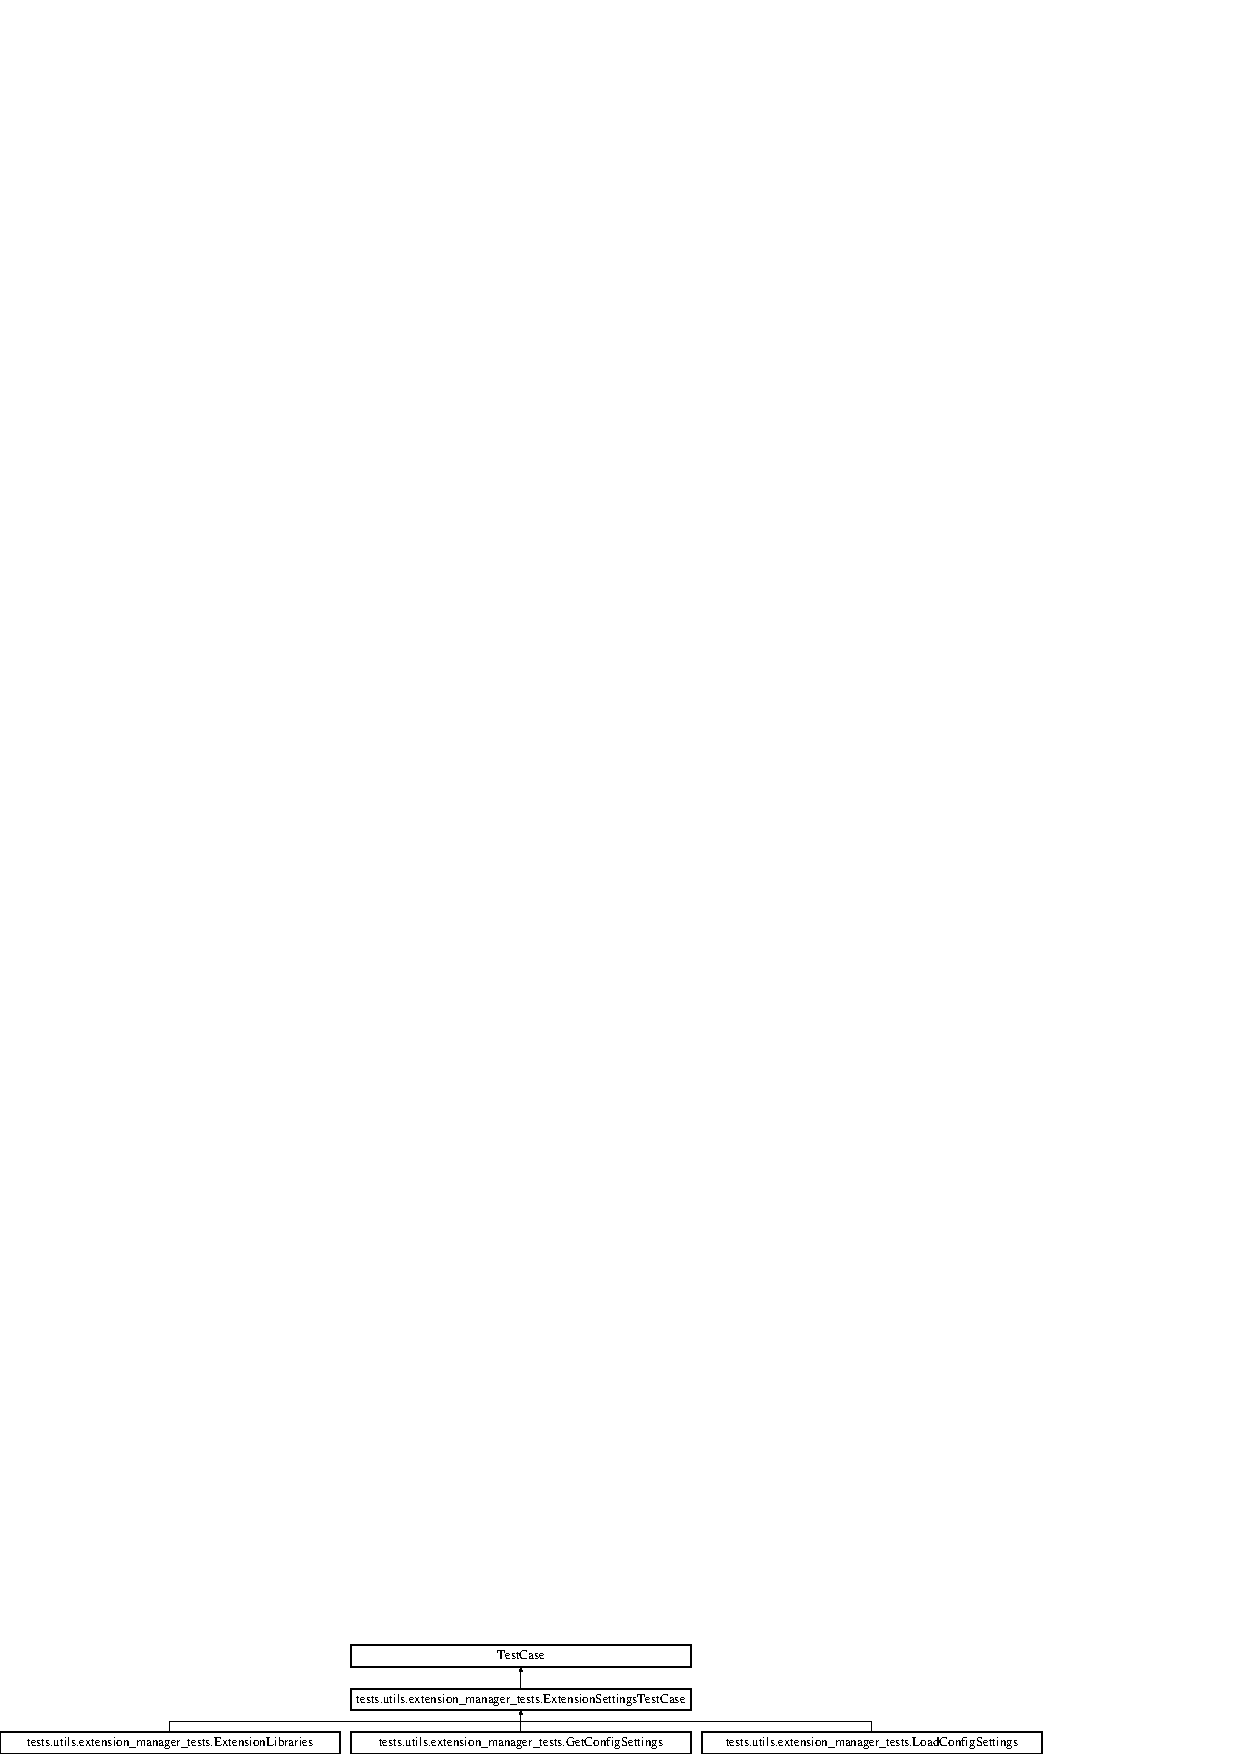
\includegraphics[height=1.513514cm]{classtests_1_1utils_1_1extension__manager__tests_1_1ExtensionSettingsTestCase}
\end{center}
\end{figure}
\subsection*{Public Member Functions}
\begin{DoxyCompactItemize}
\item 
\hypertarget{classtests_1_1utils_1_1extension__manager__tests_1_1ExtensionSettingsTestCase_ada7b1ab0d0fe85c3a38392c0305aa3a5}{def {\bfseries set\+Up}}\label{classtests_1_1utils_1_1extension__manager__tests_1_1ExtensionSettingsTestCase_ada7b1ab0d0fe85c3a38392c0305aa3a5}

\item 
\hypertarget{classtests_1_1utils_1_1extension__manager__tests_1_1ExtensionSettingsTestCase_a16facc5e00ba98e9410c3e8d2c42bb89}{def {\bfseries tear\+Down}}\label{classtests_1_1utils_1_1extension__manager__tests_1_1ExtensionSettingsTestCase_a16facc5e00ba98e9410c3e8d2c42bb89}

\end{DoxyCompactItemize}
\subsection*{Public Attributes}
\begin{DoxyCompactItemize}
\item 
\hypertarget{classtests_1_1utils_1_1extension__manager__tests_1_1ExtensionSettingsTestCase_ad69eeb2a244780bb42fa81a4a5eca1b7}{{\bfseries app}}\label{classtests_1_1utils_1_1extension__manager__tests_1_1ExtensionSettingsTestCase_ad69eeb2a244780bb42fa81a4a5eca1b7}

\item 
\hypertarget{classtests_1_1utils_1_1extension__manager__tests_1_1ExtensionSettingsTestCase_ac2c652333c649703f486eeaf7233c3c9}{{\bfseries ext\+\_\+mgr}}\label{classtests_1_1utils_1_1extension__manager__tests_1_1ExtensionSettingsTestCase_ac2c652333c649703f486eeaf7233c3c9}

\end{DoxyCompactItemize}


The documentation for this class was generated from the following file\+:\begin{DoxyCompactItemize}
\item 
tests/utils/extension\+\_\+manager\+\_\+tests.\+py\end{DoxyCompactItemize}

\hypertarget{classcommotion__client_1_1GUI_1_1extension__toolbar_1_1ExtensionToolBar}{\section{commotion\+\_\+client.\+G\+U\+I.\+extension\+\_\+toolbar.\+Extension\+Tool\+Bar Class Reference}
\label{classcommotion__client_1_1GUI_1_1extension__toolbar_1_1ExtensionToolBar}\index{commotion\+\_\+client.\+G\+U\+I.\+extension\+\_\+toolbar.\+Extension\+Tool\+Bar@{commotion\+\_\+client.\+G\+U\+I.\+extension\+\_\+toolbar.\+Extension\+Tool\+Bar}}
}
Inheritance diagram for commotion\+\_\+client.\+G\+U\+I.\+extension\+\_\+toolbar.\+Extension\+Tool\+Bar\+:\begin{figure}[H]
\begin{center}
\leavevmode
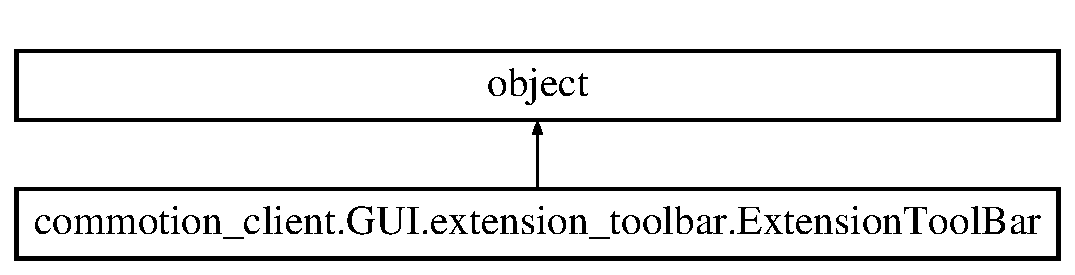
\includegraphics[height=2.000000cm]{classcommotion__client_1_1GUI_1_1extension__toolbar_1_1ExtensionToolBar}
\end{center}
\end{figure}
\subsection*{Public Member Functions}
\begin{DoxyCompactItemize}
\item 
def \hyperlink{classcommotion__client_1_1GUI_1_1extension__toolbar_1_1ExtensionToolBar_a29e92f0e66f5f056be55e3a5ef7f2fd8}{\+\_\+\+\_\+init\+\_\+\+\_\+}
\item 
\hypertarget{classcommotion__client_1_1GUI_1_1extension__toolbar_1_1ExtensionToolBar_a82e5c75a5e699eb6dd86810dab2b43a8}{def {\bfseries add\+\_\+item}}\label{classcommotion__client_1_1GUI_1_1extension__toolbar_1_1ExtensionToolBar_a82e5c75a5e699eb6dd86810dab2b43a8}

\end{DoxyCompactItemize}
\subsection*{Public Attributes}
\begin{DoxyCompactItemize}
\item 
\hypertarget{classcommotion__client_1_1GUI_1_1extension__toolbar_1_1ExtensionToolBar_a6319ad6aa6c0480e17413b5c8a018d5f}{{\bfseries log}}\label{classcommotion__client_1_1GUI_1_1extension__toolbar_1_1ExtensionToolBar_a6319ad6aa6c0480e17413b5c8a018d5f}

\item 
\hypertarget{classcommotion__client_1_1GUI_1_1extension__toolbar_1_1ExtensionToolBar_ad52b111af7587b8ed8fb2e1703f8251b}{{\bfseries translate}}\label{classcommotion__client_1_1GUI_1_1extension__toolbar_1_1ExtensionToolBar_ad52b111af7587b8ed8fb2e1703f8251b}

\item 
\hypertarget{classcommotion__client_1_1GUI_1_1extension__toolbar_1_1ExtensionToolBar_ae4fb6875e8968fb1b48a516117ee010f}{{\bfseries viewport}}\label{classcommotion__client_1_1GUI_1_1extension__toolbar_1_1ExtensionToolBar_ae4fb6875e8968fb1b48a516117ee010f}

\item 
\hypertarget{classcommotion__client_1_1GUI_1_1extension__toolbar_1_1ExtensionToolBar_a4c951281d81006ea5a1603030f4fa799}{{\bfseries menu\+\_\+items}}\label{classcommotion__client_1_1GUI_1_1extension__toolbar_1_1ExtensionToolBar_a4c951281d81006ea5a1603030f4fa799}

\item 
\hypertarget{classcommotion__client_1_1GUI_1_1extension__toolbar_1_1ExtensionToolBar_afa628724b1895e1fe4f5bd5605ead016}{{\bfseries icon}}\label{classcommotion__client_1_1GUI_1_1extension__toolbar_1_1ExtensionToolBar_afa628724b1895e1fe4f5bd5605ead016}

\end{DoxyCompactItemize}


\subsection{Detailed Description}
\begin{DoxyVerb}The central widget for the commotion client. This widget initalizes all other sub-widgets and extensions as well as defines the paramiters of the main GUI container.


An example of adding a single button to the menu that calls a function "save_form()"

new_button = MenuItem
my_button.setIcon(icon.save)
my_button.setText(self.translate("menu", "Save"))
new_button.action = self.save_form
self.add_item(new_button)\end{DoxyVerb}
 

\subsection{Constructor \& Destructor Documentation}
\hypertarget{classcommotion__client_1_1GUI_1_1extension__toolbar_1_1ExtensionToolBar_a29e92f0e66f5f056be55e3a5ef7f2fd8}{\index{commotion\+\_\+client\+::\+G\+U\+I\+::extension\+\_\+toolbar\+::\+Extension\+Tool\+Bar@{commotion\+\_\+client\+::\+G\+U\+I\+::extension\+\_\+toolbar\+::\+Extension\+Tool\+Bar}!\+\_\+\+\_\+init\+\_\+\+\_\+@{\+\_\+\+\_\+init\+\_\+\+\_\+}}
\index{\+\_\+\+\_\+init\+\_\+\+\_\+@{\+\_\+\+\_\+init\+\_\+\+\_\+}!commotion\+\_\+client\+::\+G\+U\+I\+::extension\+\_\+toolbar\+::\+Extension\+Tool\+Bar@{commotion\+\_\+client\+::\+G\+U\+I\+::extension\+\_\+toolbar\+::\+Extension\+Tool\+Bar}}
\subsubsection[{\+\_\+\+\_\+init\+\_\+\+\_\+}]{\setlength{\rightskip}{0pt plus 5cm}def commotion\+\_\+client.\+G\+U\+I.\+extension\+\_\+toolbar.\+Extension\+Tool\+Bar.\+\_\+\+\_\+init\+\_\+\+\_\+ (
\begin{DoxyParamCaption}
\item[{}]{self, }
\item[{}]{viewport}
\end{DoxyParamCaption}
)}}\label{classcommotion__client_1_1GUI_1_1extension__toolbar_1_1ExtensionToolBar_a29e92f0e66f5f056be55e3a5ef7f2fd8}
\begin{DoxyVerb}Sets up all the translation, logging, and core items needed for an extension toolbar.

Args:
  extension_menu_items (object): The extension specific menu-item to be used by an extension. This class is derived from the  
  viewport (object): The extensions viewport. This allows menu_items to have its actions interact with the current viewport.        
\end{DoxyVerb}
 

References commotion\+\_\+client.\+G\+U\+I.\+extension\+\_\+toolbar.\+Extension\+Tool\+Bar.\+\_\+dirty, commotion\+\_\+client.\+extensions.\+config\+\_\+editor.\+main.\+View\+Port.\+\_\+dirty, commotion\+\_\+client.\+G\+U\+I.\+extension\+\_\+toolbar.\+Extension\+Tool\+Bar.\+icon, commotion\+\_\+client.\+G\+U\+I.\+crash\+\_\+report.\+Crash\+Report.\+log, commotion\+\_\+client.\+extensions.\+config\+\_\+editor.\+main.\+View\+Port.\+log, commotion\+\_\+client.\+G\+U\+I.\+extension\+\_\+toolbar.\+Extension\+Tool\+Bar.\+log, commotion\+\_\+client.\+commotion\+\_\+client.\+Hold\+State\+During\+Restart.\+log, commotion\+\_\+client.\+G\+U\+I.\+crash\+\_\+report.\+Report\+Gatherer.\+log, commotion\+\_\+client.\+commotion\+\_\+client.\+Commotion\+Client\+Application.\+log, commotion\+\_\+client.\+G\+U\+I.\+extension\+\_\+toolbar.\+Extension\+Tool\+Bar.\+menu\+\_\+items, commotion\+\_\+client.\+extensions.\+config\+\_\+editor.\+main.\+View\+Port.\+translate, commotion\+\_\+client.\+G\+U\+I.\+extension\+\_\+toolbar.\+Extension\+Tool\+Bar.\+translate, commotion\+\_\+client.\+commotion\+\_\+client.\+Commotion\+Client\+Application.\+translate, and commotion\+\_\+client.\+G\+U\+I.\+extension\+\_\+toolbar.\+Extension\+Tool\+Bar.\+viewport.


\begin{DoxyCode}
36 
37     \textcolor{keyword}{def }\hyperlink{classcommotion__client_1_1GUI_1_1extension__toolbar_1_1ExtensionToolBar_a29e92f0e66f5f056be55e3a5ef7f2fd8}{\_\_init\_\_}(self, viewport):
38         \textcolor{stringliteral}{"""Sets up all the translation, logging, and core items needed for an extension toolbar.}
39 \textcolor{stringliteral}{        }
40 \textcolor{stringliteral}{        Args:}
41 \textcolor{stringliteral}{          extension\_menu\_items (object): The extension specific menu-item to be used by an extension. This
       class is derived from the  }
42 \textcolor{stringliteral}{          viewport (object): The extensions viewport. This allows menu\_items to have its actions interact
       with the current viewport.        }
43 \textcolor{stringliteral}{        """}
44         super().\hyperlink{classcommotion__client_1_1GUI_1_1extension__toolbar_1_1ExtensionToolBar_a29e92f0e66f5f056be55e3a5ef7f2fd8}{\_\_init\_\_}()
45         self.\hyperlink{classcommotion__client_1_1GUI_1_1extension__toolbar_1_1ExtensionToolBar_a84233fa2bbebfb96f4c6c490487b4f87}{\_dirty} = \textcolor{keyword}{False}
46         self.\hyperlink{classcommotion__client_1_1GUI_1_1extension__toolbar_1_1ExtensionToolBar_a6319ad6aa6c0480e17413b5c8a018d5f}{log} = logging.getLogger(\textcolor{stringliteral}{"commotion\_client."}+\_\_name\_\_)
47         self.\hyperlink{classcommotion__client_1_1GUI_1_1extension__toolbar_1_1ExtensionToolBar_ad52b111af7587b8ed8fb2e1703f8251b}{translate} = QtCore.QCoreApplication.translate
48         self.\hyperlink{classcommotion__client_1_1GUI_1_1extension__toolbar_1_1ExtensionToolBar_ae4fb6875e8968fb1b48a516117ee010f}{viewport} = viewport
49         self.\hyperlink{classcommotion__client_1_1GUI_1_1extension__toolbar_1_1ExtensionToolBar_a4c951281d81006ea5a1603030f4fa799}{menu\_items} = \{\}
50         \textcolor{comment}{#The basic set of icons for extensions}
51         self.\hyperlink{classcommotion__client_1_1GUI_1_1extension__toolbar_1_1ExtensionToolBar_afa628724b1895e1fe4f5bd5605ead016}{icon} = \{
52             \textcolor{stringliteral}{"save"}:QtGui.QIcon(\textcolor{stringliteral}{":save32.png"}),
53             \textcolor{stringliteral}{"load"}:QtGui.QIcon(\textcolor{stringliteral}{":load32.png"}),
54             \textcolor{stringliteral}{"user"}:QtGui.QIcon(\textcolor{stringliteral}{":user32.png"}),
55             \textcolor{stringliteral}{"settings"}:QtGui.QIcon(\textcolor{stringliteral}{":settings32.png"}),
56             \textcolor{stringliteral}{"full\_screen\_start"}:QtGui.QIcon(\textcolor{stringliteral}{":full\_screen\_start32.png"}),
57             \textcolor{stringliteral}{"full\_screen\_end"}:QtGui.QIcon(\textcolor{stringliteral}{":full\_screen\_end32.png"}),
58         \}

\end{DoxyCode}


The documentation for this class was generated from the following file\+:\begin{DoxyCompactItemize}
\item 
commotion\+\_\+client/\+G\+U\+I/extension\+\_\+toolbar.\+py\end{DoxyCompactItemize}

\hypertarget{classcommotion__client_1_1utils_1_1thread_1_1GenericThread}{\section{commotion\+\_\+client.\+utils.\+thread.\+Generic\+Thread Class Reference}
\label{classcommotion__client_1_1utils_1_1thread_1_1GenericThread}\index{commotion\+\_\+client.\+utils.\+thread.\+Generic\+Thread@{commotion\+\_\+client.\+utils.\+thread.\+Generic\+Thread}}
}
Inheritance diagram for commotion\+\_\+client.\+utils.\+thread.\+Generic\+Thread\+:\begin{figure}[H]
\begin{center}
\leavevmode
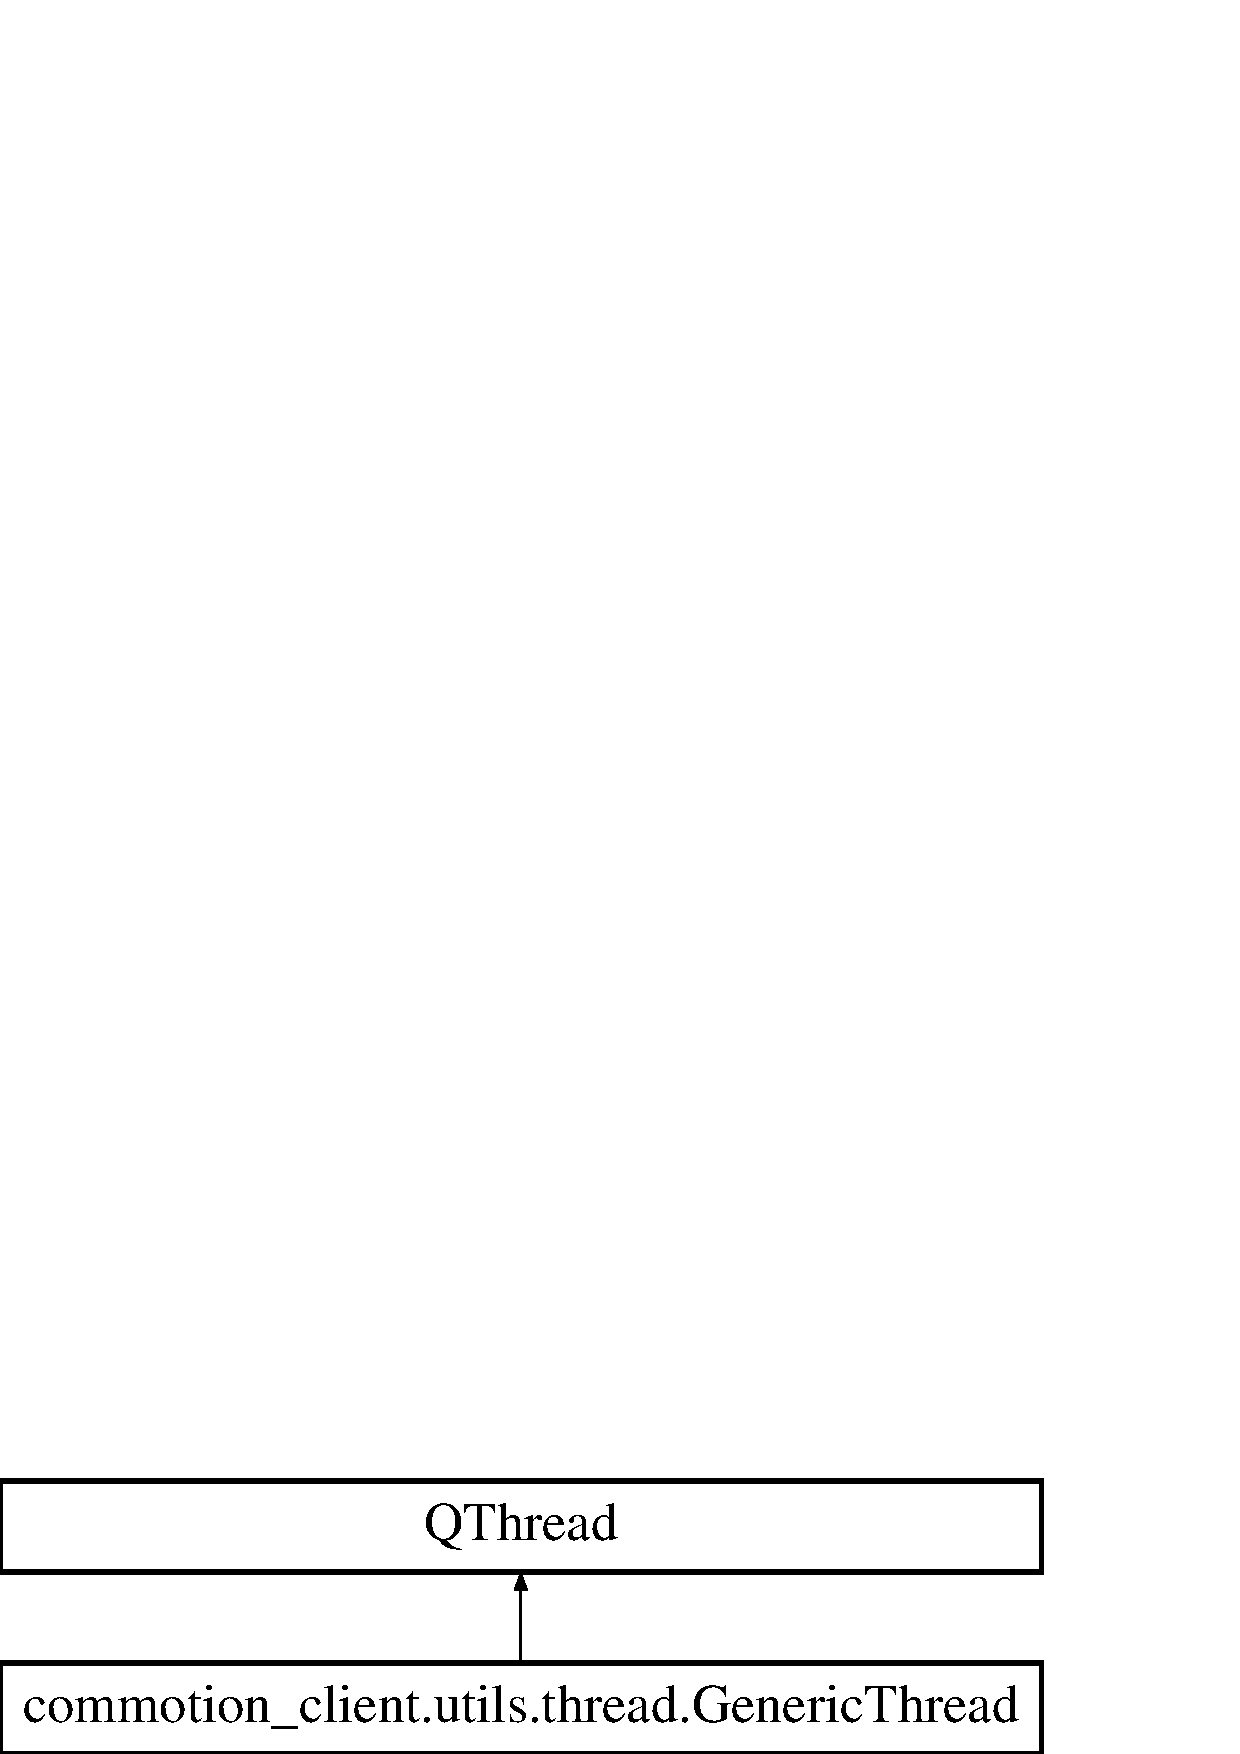
\includegraphics[height=2.000000cm]{classcommotion__client_1_1utils_1_1thread_1_1GenericThread}
\end{center}
\end{figure}
\subsection*{Public Member Functions}
\begin{DoxyCompactItemize}
\item 
\hypertarget{classcommotion__client_1_1utils_1_1thread_1_1GenericThread_a671a08f13469e8d618f36d84ce9cecbe}{def {\bfseries \+\_\+\+\_\+init\+\_\+\+\_\+}}\label{classcommotion__client_1_1utils_1_1thread_1_1GenericThread_a671a08f13469e8d618f36d84ce9cecbe}

\end{DoxyCompactItemize}
\subsection*{Public Attributes}
\begin{DoxyCompactItemize}
\item 
\hypertarget{classcommotion__client_1_1utils_1_1thread_1_1GenericThread_ad7535d8328a50a61385d8b5f58435f0c}{{\bfseries log}}\label{classcommotion__client_1_1utils_1_1thread_1_1GenericThread_ad7535d8328a50a61385d8b5f58435f0c}

\end{DoxyCompactItemize}


The documentation for this class was generated from the following file\+:\begin{DoxyCompactItemize}
\item 
commotion\+\_\+client/utils/thread.\+py\end{DoxyCompactItemize}

\hypertarget{classtests_1_1utils_1_1extension__manager__tests_1_1GetConfigSettings}{\section{tests.\+utils.\+extension\+\_\+manager\+\_\+tests.\+Get\+Config\+Settings Class Reference}
\label{classtests_1_1utils_1_1extension__manager__tests_1_1GetConfigSettings}\index{tests.\+utils.\+extension\+\_\+manager\+\_\+tests.\+Get\+Config\+Settings@{tests.\+utils.\+extension\+\_\+manager\+\_\+tests.\+Get\+Config\+Settings}}
}
Inheritance diagram for tests.\+utils.\+extension\+\_\+manager\+\_\+tests.\+Get\+Config\+Settings\+:\begin{figure}[H]
\begin{center}
\leavevmode
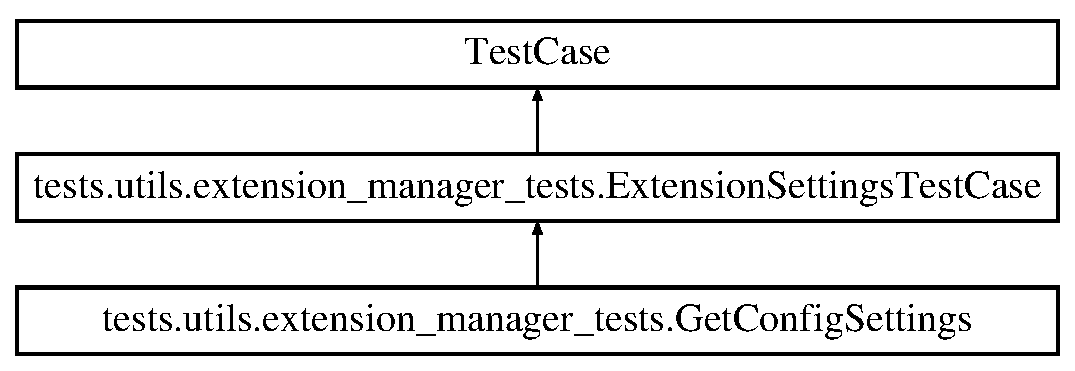
\includegraphics[height=3.000000cm]{classtests_1_1utils_1_1extension__manager__tests_1_1GetConfigSettings}
\end{center}
\end{figure}
\subsection*{Public Member Functions}
\begin{DoxyCompactItemize}
\item 
def \hyperlink{classtests_1_1utils_1_1extension__manager__tests_1_1GetConfigSettings_abb00849dbf033d220046921187102261}{test\+\_\+get\+\_\+installed}
\item 
def \hyperlink{classtests_1_1utils_1_1extension__manager__tests_1_1GetConfigSettings_ad7405dd268be73fd701a305f057b6443}{test\+\_\+check\+\_\+installed}
\end{DoxyCompactItemize}
\subsection*{Additional Inherited Members}


\subsection{Member Function Documentation}
\hypertarget{classtests_1_1utils_1_1extension__manager__tests_1_1GetConfigSettings_ad7405dd268be73fd701a305f057b6443}{\index{tests\+::utils\+::extension\+\_\+manager\+\_\+tests\+::\+Get\+Config\+Settings@{tests\+::utils\+::extension\+\_\+manager\+\_\+tests\+::\+Get\+Config\+Settings}!test\+\_\+check\+\_\+installed@{test\+\_\+check\+\_\+installed}}
\index{test\+\_\+check\+\_\+installed@{test\+\_\+check\+\_\+installed}!tests\+::utils\+::extension\+\_\+manager\+\_\+tests\+::\+Get\+Config\+Settings@{tests\+::utils\+::extension\+\_\+manager\+\_\+tests\+::\+Get\+Config\+Settings}}
\subsubsection[{test\+\_\+check\+\_\+installed}]{\setlength{\rightskip}{0pt plus 5cm}def tests.\+utils.\+extension\+\_\+manager\+\_\+tests.\+Get\+Config\+Settings.\+test\+\_\+check\+\_\+installed (
\begin{DoxyParamCaption}
\item[{}]{self}
\end{DoxyParamCaption}
)}}\label{classtests_1_1utils_1_1extension__manager__tests_1_1GetConfigSettings_ad7405dd268be73fd701a305f057b6443}
\begin{DoxyVerb}Test that get_installed function properly checks & returns if extensions are installed.\end{DoxyVerb}
 
\begin{DoxyCode}
155 
156     \textcolor{keyword}{def }\hyperlink{classtests_1_1utils_1_1extension__manager__tests_1_1GetConfigSettings_ad7405dd268be73fd701a305f057b6443}{test\_check\_installed}(self):
157         \textcolor{stringliteral}{"""Test that get\_installed function properly checks & returns if extensions are installed."""}
158         \textcolor{comment}{#test empty first}
159         self.assertFalse(self.ext\_mgr.check\_installed())
160         self.assertFalse(self.ext\_mgr.check\_installed(\textcolor{stringliteral}{"test"}))
161         \textcolor{comment}{#add a value to settings}
162         self.ext\_mgr.user\_settings.setValue(\textcolor{stringliteral}{"test/type"}, \textcolor{stringliteral}{"global"})
163         self.ext\_mgr.user\_settings.sync()
164         self.assertTrue(self.ext\_mgr.check\_installed())
165         self.assertTrue(self.ext\_mgr.check\_installed(\textcolor{stringliteral}{"test"}))
166         self.assertFalse(self.ext\_mgr.check\_installed(\textcolor{stringliteral}{"pineapple"}))

\end{DoxyCode}
\hypertarget{classtests_1_1utils_1_1extension__manager__tests_1_1GetConfigSettings_abb00849dbf033d220046921187102261}{\index{tests\+::utils\+::extension\+\_\+manager\+\_\+tests\+::\+Get\+Config\+Settings@{tests\+::utils\+::extension\+\_\+manager\+\_\+tests\+::\+Get\+Config\+Settings}!test\+\_\+get\+\_\+installed@{test\+\_\+get\+\_\+installed}}
\index{test\+\_\+get\+\_\+installed@{test\+\_\+get\+\_\+installed}!tests\+::utils\+::extension\+\_\+manager\+\_\+tests\+::\+Get\+Config\+Settings@{tests\+::utils\+::extension\+\_\+manager\+\_\+tests\+::\+Get\+Config\+Settings}}
\subsubsection[{test\+\_\+get\+\_\+installed}]{\setlength{\rightskip}{0pt plus 5cm}def tests.\+utils.\+extension\+\_\+manager\+\_\+tests.\+Get\+Config\+Settings.\+test\+\_\+get\+\_\+installed (
\begin{DoxyParamCaption}
\item[{}]{self}
\end{DoxyParamCaption}
)}}\label{classtests_1_1utils_1_1extension__manager__tests_1_1GetConfigSettings_abb00849dbf033d220046921187102261}
\begin{DoxyVerb}Test that get_installed function properly checks & returns installed extensions.\end{DoxyVerb}
 
\begin{DoxyCode}
143 
144     \textcolor{keyword}{def }\hyperlink{classtests_1_1utils_1_1extension__manager__tests_1_1GetConfigSettings_abb00849dbf033d220046921187102261}{test\_get\_installed}(self):
145         \textcolor{stringliteral}{"""Test that get\_installed function properly checks & returns installed extensions."""}
146         empty\_inst = self.ext\_mgr.get\_installed()
147         self.assertEqual(empty\_inst, \{\})
148         \textcolor{comment}{#add a value to settings}
149         self.ext\_mgr.user\_settings.setValue(\textcolor{stringliteral}{"test/type"}, \textcolor{stringliteral}{"global"})
150         self.ext\_mgr.user\_settings.sync()
151         one\_item = self.ext\_mgr.get\_installed()
152         self.assertEqual(len(one\_item), 1)
153         self.assertIn(\textcolor{stringliteral}{"test"}, one\_item)
154         self.assertEqual(one\_item[\textcolor{stringliteral}{'test'}], \textcolor{stringliteral}{'global'})
 
\end{DoxyCode}


The documentation for this class was generated from the following file\+:\begin{DoxyCompactItemize}
\item 
tests/utils/extension\+\_\+manager\+\_\+tests.\+py\end{DoxyCompactItemize}

\hypertarget{classcommotion__client_1_1commotion__client_1_1HoldStateDuringRestart}{\section{commotion\-\_\-client.\-commotion\-\_\-client.\-Hold\-State\-During\-Restart Class Reference}
\label{classcommotion__client_1_1commotion__client_1_1HoldStateDuringRestart}\index{commotion\-\_\-client.\-commotion\-\_\-client.\-Hold\-State\-During\-Restart@{commotion\-\_\-client.\-commotion\-\_\-client.\-Hold\-State\-During\-Restart}}
}
Inheritance diagram for commotion\-\_\-client.\-commotion\-\_\-client.\-Hold\-State\-During\-Restart\-:\begin{figure}[H]
\begin{center}
\leavevmode
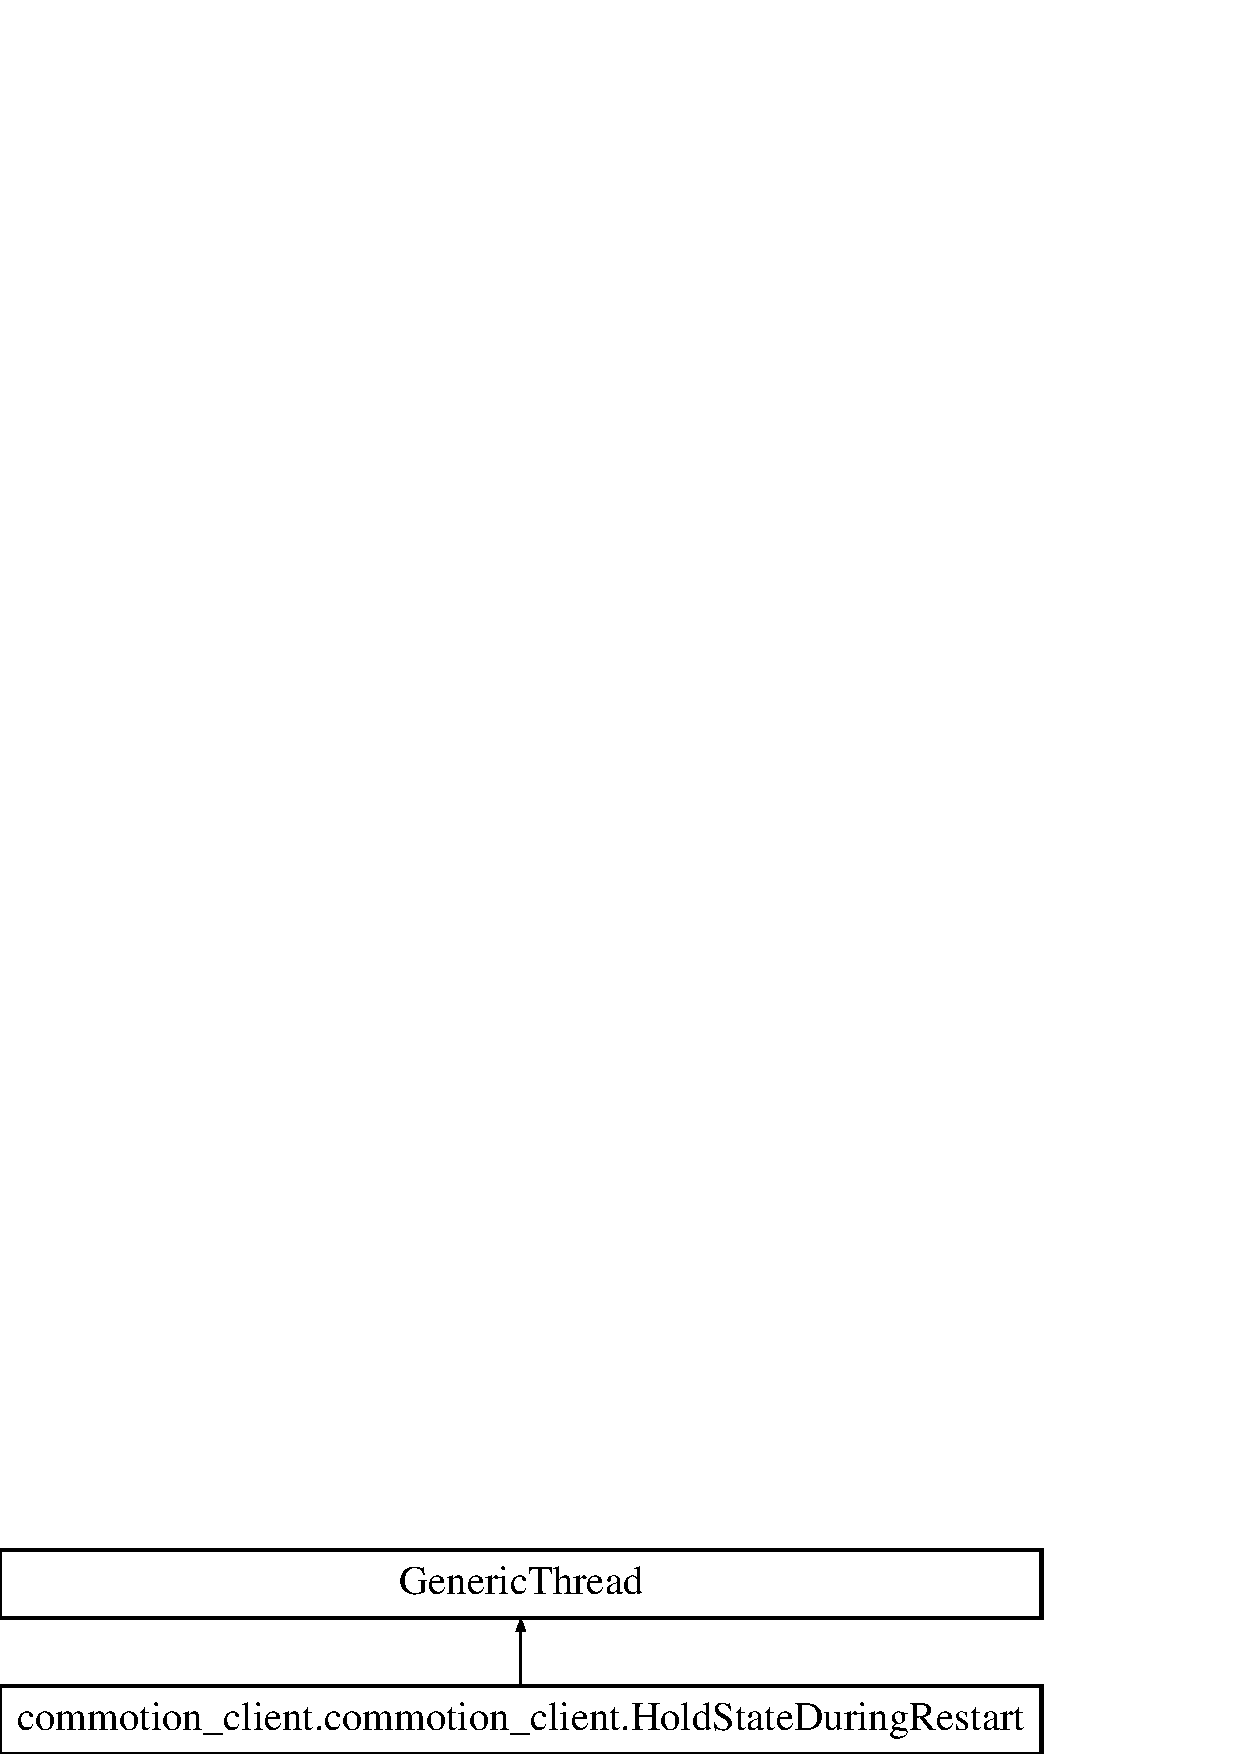
\includegraphics[height=2.000000cm]{classcommotion__client_1_1commotion__client_1_1HoldStateDuringRestart}
\end{center}
\end{figure}
\subsection*{Public Member Functions}
\begin{DoxyCompactItemize}
\item 
\hypertarget{classcommotion__client_1_1commotion__client_1_1HoldStateDuringRestart_a94f6059b8470ee3a2307bdc2d08935a4}{def {\bfseries \-\_\-\-\_\-init\-\_\-\-\_\-}}\label{classcommotion__client_1_1commotion__client_1_1HoldStateDuringRestart_a94f6059b8470ee3a2307bdc2d08935a4}

\item 
\hypertarget{classcommotion__client_1_1commotion__client_1_1HoldStateDuringRestart_a8f5151ef8eaea8fbdaa3d52005556ad2}{def {\bfseries end}}\label{classcommotion__client_1_1commotion__client_1_1HoldStateDuringRestart_a8f5151ef8eaea8fbdaa3d52005556ad2}

\item 
\hypertarget{classcommotion__client_1_1commotion__client_1_1HoldStateDuringRestart_a4385fc3adbd39cb53ad032166fac2aef}{def {\bfseries run}}\label{classcommotion__client_1_1commotion__client_1_1HoldStateDuringRestart_a4385fc3adbd39cb53ad032166fac2aef}

\end{DoxyCompactItemize}
\subsection*{Public Attributes}
\begin{DoxyCompactItemize}
\item 
\hypertarget{classcommotion__client_1_1commotion__client_1_1HoldStateDuringRestart_ad49b6b600ca627a0498a372f15887859}{{\bfseries restart\-\_\-complete}}\label{classcommotion__client_1_1commotion__client_1_1HoldStateDuringRestart_ad49b6b600ca627a0498a372f15887859}

\item 
\hypertarget{classcommotion__client_1_1commotion__client_1_1HoldStateDuringRestart_a999d8455148ca332ec899dfe79585423}{{\bfseries log}}\label{classcommotion__client_1_1commotion__client_1_1HoldStateDuringRestart_a999d8455148ca332ec899dfe79585423}

\end{DoxyCompactItemize}


\subsection{Detailed Description}
\begin{DoxyVerb}A thread that will run during the restart of all other components to keep the applicaiton alive.
\end{DoxyVerb}
 

The documentation for this class was generated from the following file\-:\begin{DoxyCompactItemize}
\item 
commotion\-\_\-client/commotion\-\_\-client.\-py\end{DoxyCompactItemize}

\hypertarget{classtests_1_1utils_1_1extension__manager__tests_1_1LoadConfigSettings}{\section{tests.\-utils.\-extension\-\_\-manager\-\_\-tests.\-Load\-Config\-Settings Class Reference}
\label{classtests_1_1utils_1_1extension__manager__tests_1_1LoadConfigSettings}\index{tests.\-utils.\-extension\-\_\-manager\-\_\-tests.\-Load\-Config\-Settings@{tests.\-utils.\-extension\-\_\-manager\-\_\-tests.\-Load\-Config\-Settings}}
}
Inheritance diagram for tests.\-utils.\-extension\-\_\-manager\-\_\-tests.\-Load\-Config\-Settings\-:\begin{figure}[H]
\begin{center}
\leavevmode
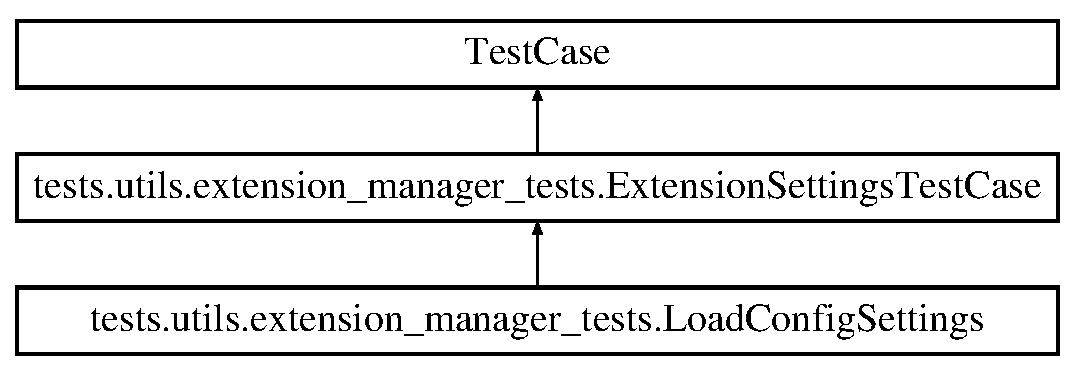
\includegraphics[height=3.000000cm]{classtests_1_1utils_1_1extension__manager__tests_1_1LoadConfigSettings}
\end{center}
\end{figure}
\subsection*{Public Member Functions}
\begin{DoxyCompactItemize}
\item 
def \hyperlink{classtests_1_1utils_1_1extension__manager__tests_1_1LoadConfigSettings_a6a030c80c178c3d3f0ca0ad4603121c1}{test\-\_\-load\-\_\-core\-\_\-ext}
\item 
def \hyperlink{classtests_1_1utils_1_1extension__manager__tests_1_1LoadConfigSettings_ad545de88fc2f5eba813161fa4cb31d83}{test\-\_\-init\-\_\-extension\-\_\-config}
\end{DoxyCompactItemize}
\subsection*{Additional Inherited Members}


\subsection{Detailed Description}
\begin{DoxyVerb}Functions Covered:
  load_all
  init_extension_config\end{DoxyVerb}
 

\subsection{Member Function Documentation}
\hypertarget{classtests_1_1utils_1_1extension__manager__tests_1_1LoadConfigSettings_ad545de88fc2f5eba813161fa4cb31d83}{\index{tests\-::utils\-::extension\-\_\-manager\-\_\-tests\-::\-Load\-Config\-Settings@{tests\-::utils\-::extension\-\_\-manager\-\_\-tests\-::\-Load\-Config\-Settings}!test\-\_\-init\-\_\-extension\-\_\-config@{test\-\_\-init\-\_\-extension\-\_\-config}}
\index{test\-\_\-init\-\_\-extension\-\_\-config@{test\-\_\-init\-\_\-extension\-\_\-config}!tests::utils::extension_manager_tests::LoadConfigSettings@{tests\-::utils\-::extension\-\_\-manager\-\_\-tests\-::\-Load\-Config\-Settings}}
\subsubsection[{test\-\_\-init\-\_\-extension\-\_\-config}]{\setlength{\rightskip}{0pt plus 5cm}def tests.\-utils.\-extension\-\_\-manager\-\_\-tests.\-Load\-Config\-Settings.\-test\-\_\-init\-\_\-extension\-\_\-config (
\begin{DoxyParamCaption}
\item[{}]{self}
\end{DoxyParamCaption}
)}}\label{classtests_1_1utils_1_1extension__manager__tests_1_1LoadConfigSettings_ad545de88fc2f5eba813161fa4cb31d83}
\begin{DoxyVerb}Test that init extension config properly handles the various use cases.\end{DoxyVerb}
 
\begin{DoxyCode}
111 
112     \textcolor{keyword}{def }\hyperlink{classtests_1_1utils_1_1extension__manager__tests_1_1LoadConfigSettings_ad545de88fc2f5eba813161fa4cb31d83}{test\_init\_extension\_config}(self):
113         \textcolor{stringliteral}{"""Test that init extension config properly handles the various use cases."""}
114         \textcolor{comment}{#ext\_type MUST be core|global|user}
115         with self.assertRaises(ValueError):
116             self.ext\_mgr.init\_extension\_config(\textcolor{stringliteral}{'pineapple'})
117 
118         \textcolor{comment}{#Check that an empty directory does nothing.}
119         self.ext\_mgr.libraries[\textcolor{stringliteral}{'user'}] = os.path.abspath(\textcolor{stringliteral}{"tests/temp/"})
120         self.ext\_mgr.init\_extension\_config(\textcolor{stringliteral}{'user'})
121         with self.assertRaises(KeyError):
122             self.ext\_mgr.extensions[\textcolor{stringliteral}{'user'}].has\_configs()
123 
124         \textcolor{comment}{#populate with populated directory}
125         self.ext\_mgr.libraries[\textcolor{stringliteral}{'user'}] = os.path.abspath(\textcolor{stringliteral}{"tests/mock/extensions/"})
126         self.ext\_mgr.init\_extension\_config(\textcolor{stringliteral}{'user'})
127         self.assertTrue(self.ext\_mgr.extensions[\textcolor{stringliteral}{'user'}].has\_configs())
128         self.ext\_mgr.extensions[\textcolor{stringliteral}{'user'}] = \textcolor{keywordtype}{None}
129         
130         \textcolor{comment}{#check all types on default call}
131         self.ext\_mgr.libraries[\textcolor{stringliteral}{'user'}] = os.path.abspath(\textcolor{stringliteral}{"tests/mock/extensions/"})
132         self.ext\_mgr.libraries[\textcolor{stringliteral}{'global'}] = os.path.abspath(\textcolor{stringliteral}{"tests/mock/extensions/"})
133         self.ext\_mgr.libraries[\textcolor{stringliteral}{'core'}] = os.path.abspath(\textcolor{stringliteral}{"tests/mock/extensions/"})
134         self.ext\_mgr.init\_extension\_config()
135         self.assertTrue(self.ext\_mgr.extensions[\textcolor{stringliteral}{'user'}].has\_configs())
136         self.assertTrue(self.ext\_mgr.extensions[\textcolor{stringliteral}{'global'}].has\_configs())
137         self.assertTrue(self.ext\_mgr.extensions[\textcolor{stringliteral}{'core'}].has\_configs())
138         self.ext\_mgr.extensions[\textcolor{stringliteral}{'user'}] = \textcolor{keywordtype}{None}
139         self.ext\_mgr.extensions[\textcolor{stringliteral}{'global'}] = \textcolor{keywordtype}{None}
140         self.ext\_mgr.extensions[\textcolor{stringliteral}{'core'}] = \textcolor{keywordtype}{None}        
        
\end{DoxyCode}
\hypertarget{classtests_1_1utils_1_1extension__manager__tests_1_1LoadConfigSettings_a6a030c80c178c3d3f0ca0ad4603121c1}{\index{tests\-::utils\-::extension\-\_\-manager\-\_\-tests\-::\-Load\-Config\-Settings@{tests\-::utils\-::extension\-\_\-manager\-\_\-tests\-::\-Load\-Config\-Settings}!test\-\_\-load\-\_\-core\-\_\-ext@{test\-\_\-load\-\_\-core\-\_\-ext}}
\index{test\-\_\-load\-\_\-core\-\_\-ext@{test\-\_\-load\-\_\-core\-\_\-ext}!tests::utils::extension_manager_tests::LoadConfigSettings@{tests\-::utils\-::extension\-\_\-manager\-\_\-tests\-::\-Load\-Config\-Settings}}
\subsubsection[{test\-\_\-load\-\_\-core\-\_\-ext}]{\setlength{\rightskip}{0pt plus 5cm}def tests.\-utils.\-extension\-\_\-manager\-\_\-tests.\-Load\-Config\-Settings.\-test\-\_\-load\-\_\-core\-\_\-ext (
\begin{DoxyParamCaption}
\item[{}]{self}
\end{DoxyParamCaption}
)}}\label{classtests_1_1utils_1_1extension__manager__tests_1_1LoadConfigSettings_a6a030c80c178c3d3f0ca0ad4603121c1}
\begin{DoxyVerb}Test that all core extension directories are loaded upon running load_core.\end{DoxyVerb}
 
\begin{DoxyCode}
97 
98     \textcolor{keyword}{def }\hyperlink{classtests_1_1utils_1_1extension__manager__tests_1_1LoadConfigSettings_a6a030c80c178c3d3f0ca0ad4603121c1}{test\_load\_core\_ext}(self):
99         \textcolor{stringliteral}{"""Test that all core extension directories are loaded upon running load\_core."""}
100         \textcolor{comment}{#get all extensions currently loaded}
101         self.ext\_mgr.libraries[\textcolor{stringliteral}{'core'}] = os.path.abspath(\textcolor{stringliteral}{"tests/mock/extensions/"})
102         self.ext\_mgr.libraries[\textcolor{stringliteral}{'global'}] = os.path.abspath(\textcolor{stringliteral}{"tests/temp/"})
103         global\_dir = QtCore.QDir(self.ext\_mgr.libraries[\textcolor{stringliteral}{'global'}])
104         global\_exts = global\_dir.entryList(QtCore.QDir.AllDirs|QtCore.QDir.NoDotAndDotDot)
105         loaded = self.ext\_mgr.load\_core()
106         self.ext\_mgr.user\_settings.beginGroup(\textcolor{stringliteral}{"extensions"})
107         k = self.ext\_mgr.user\_settings.allKeys()
108         \textcolor{keywordflow}{for} ext \textcolor{keywordflow}{in} global\_exts:
109             contains = (ext \textcolor{keywordflow}{in} k)
110             self.assertTrue(contains, \textcolor{stringliteral}{"Core extension \{0\} should have been loaded, but was not."}.format(ext
      ))

\end{DoxyCode}


The documentation for this class was generated from the following file\-:\begin{DoxyCompactItemize}
\item 
tests/utils/extension\-\_\-manager\-\_\-tests.\-py\end{DoxyCompactItemize}

\hypertarget{classcommotion__client_1_1utils_1_1logger_1_1LogHandler}{\section{commotion\-\_\-client.\-utils.\-logger.\-Log\-Handler Class Reference}
\label{classcommotion__client_1_1utils_1_1logger_1_1LogHandler}\index{commotion\-\_\-client.\-utils.\-logger.\-Log\-Handler@{commotion\-\_\-client.\-utils.\-logger.\-Log\-Handler}}
}
Inheritance diagram for commotion\-\_\-client.\-utils.\-logger.\-Log\-Handler\-:\begin{figure}[H]
\begin{center}
\leavevmode
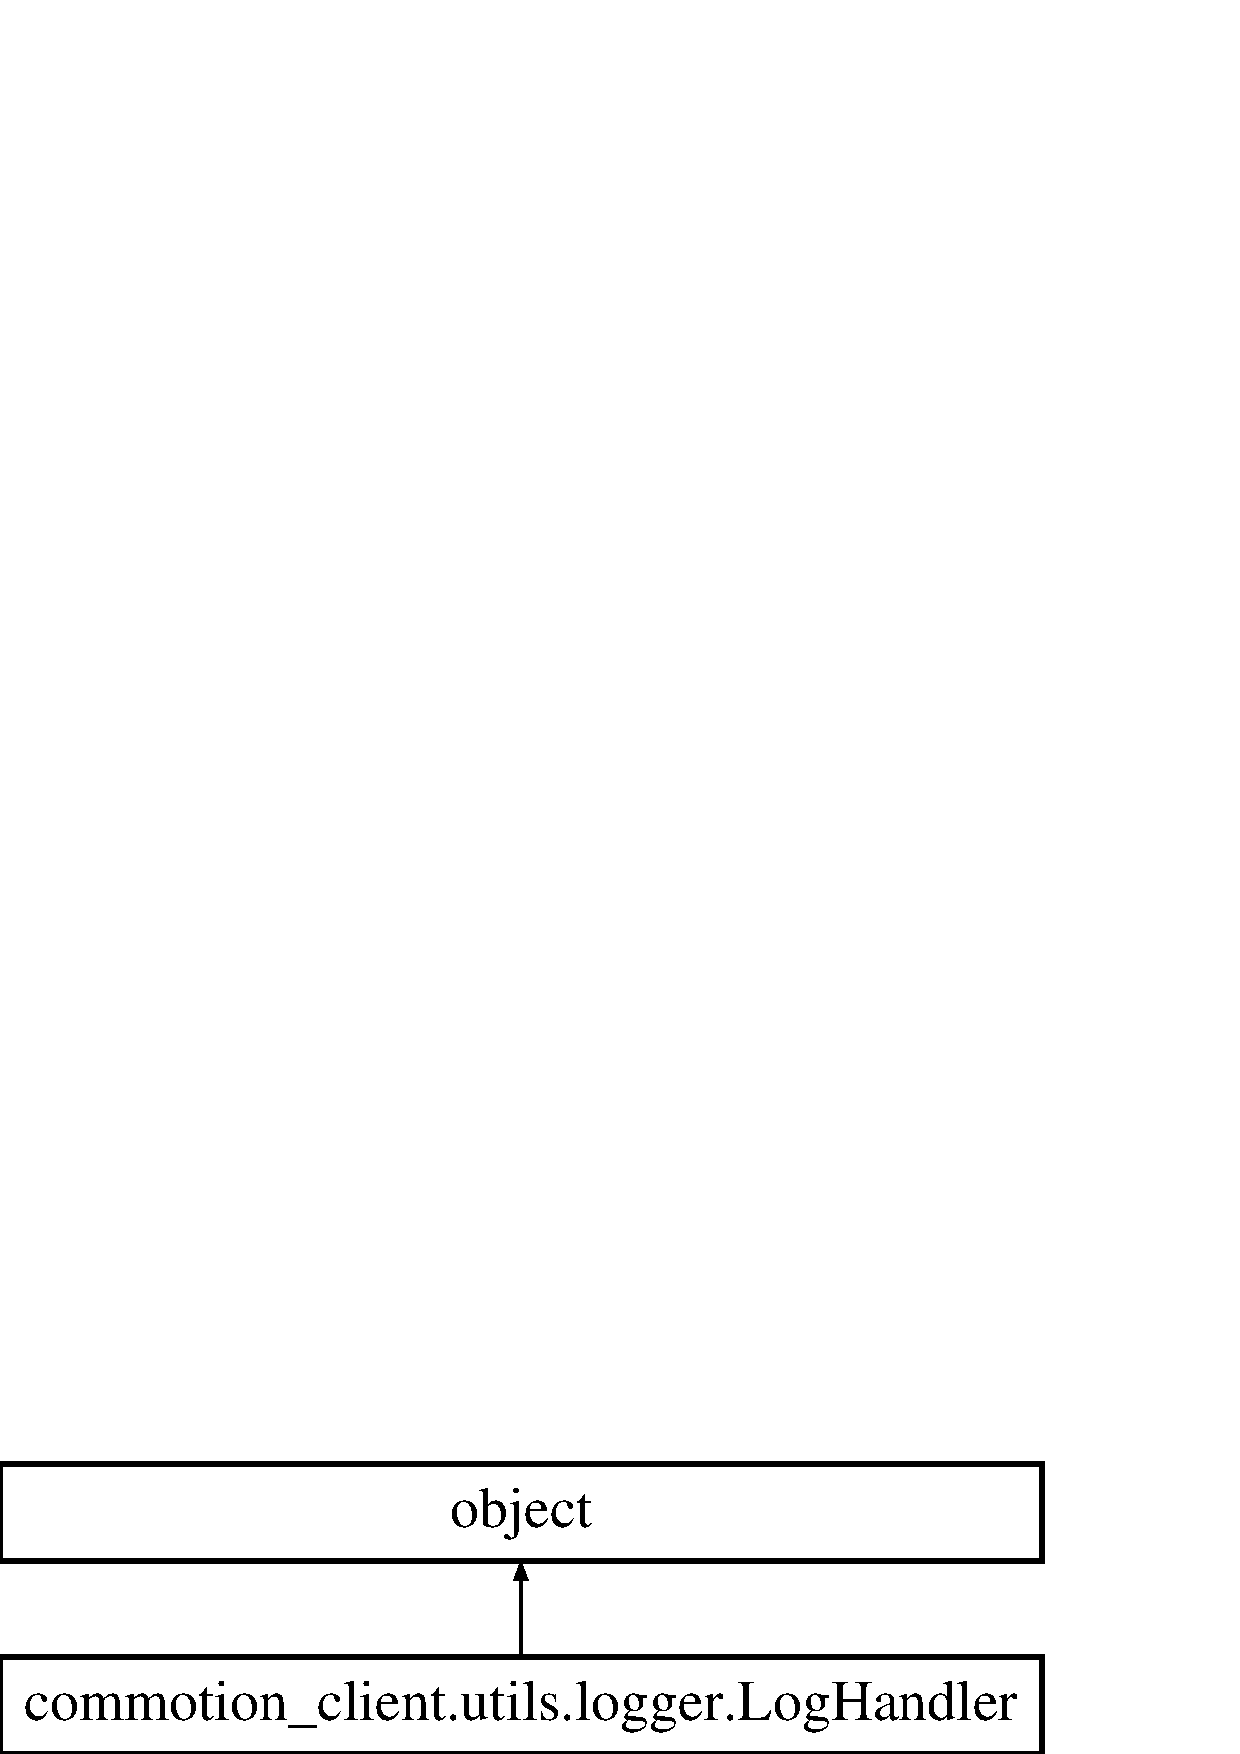
\includegraphics[height=2.000000cm]{classcommotion__client_1_1utils_1_1logger_1_1LogHandler}
\end{center}
\end{figure}
\subsection*{Public Member Functions}
\begin{DoxyCompactItemize}
\item 
\hypertarget{classcommotion__client_1_1utils_1_1logger_1_1LogHandler_a505b62933baef8f074b615aad533d059}{def {\bfseries \-\_\-\-\_\-init\-\_\-\-\_\-}}\label{classcommotion__client_1_1utils_1_1logger_1_1LogHandler_a505b62933baef8f074b615aad533d059}

\item 
def \hyperlink{classcommotion__client_1_1utils_1_1logger_1_1LogHandler_a1d1431f7384b19dc25e176361b7eeb23}{set\-\_\-logfile}
\item 
def \hyperlink{classcommotion__client_1_1utils_1_1logger_1_1LogHandler_a3d76d342b09b2d51753751e5f64f48df}{set\-\_\-verbosity}
\item 
\hypertarget{classcommotion__client_1_1utils_1_1logger_1_1LogHandler_ac9b855879e61081132fae4067b330507}{def {\bfseries get\-\_\-logger}}\label{classcommotion__client_1_1utils_1_1logger_1_1LogHandler_ac9b855879e61081132fae4067b330507}

\end{DoxyCompactItemize}
\subsection*{Public Attributes}
\begin{DoxyCompactItemize}
\item 
\hypertarget{classcommotion__client_1_1utils_1_1logger_1_1LogHandler_a56e66bd2b61cd60a8ad0e093f34ca208}{{\bfseries logger}}\label{classcommotion__client_1_1utils_1_1logger_1_1LogHandler_a56e66bd2b61cd60a8ad0e093f34ca208}

\item 
\hypertarget{classcommotion__client_1_1utils_1_1logger_1_1LogHandler_a0e8bffd460ab94f0e05bdc8a676d2c4f}{{\bfseries levels}}\label{classcommotion__client_1_1utils_1_1logger_1_1LogHandler_a0e8bffd460ab94f0e05bdc8a676d2c4f}

\item 
\hypertarget{classcommotion__client_1_1utils_1_1logger_1_1LogHandler_adbe12df7374590dd37a12eb84ee48a41}{{\bfseries formatter}}\label{classcommotion__client_1_1utils_1_1logger_1_1LogHandler_adbe12df7374590dd37a12eb84ee48a41}

\item 
\hypertarget{classcommotion__client_1_1utils_1_1logger_1_1LogHandler_a83d51d996fcf161a5b107a2589f96966}{{\bfseries stream}}\label{classcommotion__client_1_1utils_1_1logger_1_1LogHandler_a83d51d996fcf161a5b107a2589f96966}

\item 
\hypertarget{classcommotion__client_1_1utils_1_1logger_1_1LogHandler_afe5e88e544dd8855d6d1b52255e6d531}{{\bfseries file\-\_\-handler}}\label{classcommotion__client_1_1utils_1_1logger_1_1LogHandler_afe5e88e544dd8855d6d1b52255e6d531}

\item 
\hypertarget{classcommotion__client_1_1utils_1_1logger_1_1LogHandler_a92d313ddde96b6e1765514f4596f26f2}{{\bfseries logfile}}\label{classcommotion__client_1_1utils_1_1logger_1_1LogHandler_a92d313ddde96b6e1765514f4596f26f2}

\end{DoxyCompactItemize}


\subsection{Detailed Description}
\begin{DoxyVerb}Main logging controls for Commotion-Client. 

This application is ONLY to be called by the main application. This logger sets up the main namespace for all other logging to take place within. All other loggers should be the core string "commotion_client" and the packages __name__ to use inheretance from the main commotion package. This way the code in an indivdual extension will be small and will inheret the logging settings that were defined in the main application.

Example Use for ALL other modules and packages:

    from commotion-client.utils import logger
    log = logger.getLogger("commotion_client"+__name__)


NOTE: The exceptions in this function do not have translation implemented. This is that they are called before the QT application and, as such, are not pushed through QT's translation tools. This could be a mistake on the developers side, as he is a bit foggy on the specifics of QT translation. You can access the feature request at https://github.com/opentechinstitute/commotion-client/issues/24
\end{DoxyVerb}
 

\subsection{Member Function Documentation}
\hypertarget{classcommotion__client_1_1utils_1_1logger_1_1LogHandler_a1d1431f7384b19dc25e176361b7eeb23}{\index{commotion\-\_\-client\-::utils\-::logger\-::\-Log\-Handler@{commotion\-\_\-client\-::utils\-::logger\-::\-Log\-Handler}!set\-\_\-logfile@{set\-\_\-logfile}}
\index{set\-\_\-logfile@{set\-\_\-logfile}!commotion_client::utils::logger::LogHandler@{commotion\-\_\-client\-::utils\-::logger\-::\-Log\-Handler}}
\subsubsection[{set\-\_\-logfile}]{\setlength{\rightskip}{0pt plus 5cm}def commotion\-\_\-client.\-utils.\-logger.\-Log\-Handler.\-set\-\_\-logfile (
\begin{DoxyParamCaption}
\item[{}]{self, }
\item[{}]{logfile = {\ttfamily None}}
\end{DoxyParamCaption}
)}}\label{classcommotion__client_1_1utils_1_1logger_1_1LogHandler_a1d1431f7384b19dc25e176361b7eeb23}
\begin{DoxyVerb}Set the file to log to.

Args:
logfile (string): The absolute path to the file to log to.
  optional: defaults to the default system logfile path.
\end{DoxyVerb}
 

References commotion\-\_\-client.\-utils.\-logger.\-Log\-Handler.\-logfile.


\begin{DoxyCode}
60 
61     \textcolor{keyword}{def }\hyperlink{classcommotion__client_1_1utils_1_1logger_1_1LogHandler_a1d1431f7384b19dc25e176361b7eeb23}{set\_logfile}(self, logfile=None):
62         \textcolor{stringliteral}{"""Set the file to log to.}
63 \textcolor{stringliteral}{        }
64 \textcolor{stringliteral}{        Args:}
65 \textcolor{stringliteral}{        logfile (string): The absolute path to the file to log to.}
66 \textcolor{stringliteral}{          optional: defaults to the default system logfile path.}
67 \textcolor{stringliteral}{        """}
68         \textcolor{keywordflow}{if} logfile:
69             log\_dir = QtCore.QDir(os.path.dirname(logfile))
70             \textcolor{keywordflow}{if} \textcolor{keywordflow}{not} log\_dir.exists():
71                 \textcolor{keywordflow}{if} log\_dir.mkpath(log\_dir.absolutePath()):
72                     self.\hyperlink{classcommotion__client_1_1utils_1_1logger_1_1LogHandler_a92d313ddde96b6e1765514f4596f26f2}{logfile} = logfile
73         platform = sys.platform
74         \textcolor{keywordflow}{if} platform == \textcolor{stringliteral}{'darwin'}:
75             \textcolor{comment}{#Try <user>/Library/Logs first}
76             log\_dir = QtCore.QDir(os.path.join(QtCore.QDir.homePath(), \textcolor{stringliteral}{"Library"}, \textcolor{stringliteral}{"Logs"}))
77             \textcolor{comment}{#if it does not exist try and create it}
78             \textcolor{keywordflow}{if} \textcolor{keywordflow}{not} log\_dir.exists():
79                 \textcolor{keywordflow}{if} \textcolor{keywordflow}{not} log\_dir.mkpath(log\_dir.absolutePath()):
80                     \textcolor{keywordflow}{raise} NotADirectoryError(\textcolor{stringliteral}{"Attempted to set logging to the user's Commotion directory.
       The directory '<home>/.Commotion' does not exist and could not be created."})
81             self.\hyperlink{classcommotion__client_1_1utils_1_1logger_1_1LogHandler_a92d313ddde96b6e1765514f4596f26f2}{logfile} = log\_dir.filePath(\textcolor{stringliteral}{"commotion.log"})
82         \textcolor{keywordflow}{elif} platform \textcolor{keywordflow}{in} [\textcolor{stringliteral}{'win32'}, \textcolor{stringliteral}{'cygwin'}]:
83             \textcolor{comment}{#Try ../AppData/Local/Commotion first}
84             log\_dir = QtCore.QDir(os.path.join(os.getenv(\textcolor{stringliteral}{'APPDATA'}), \textcolor{stringliteral}{"Local"}, \textcolor{stringliteral}{"Commotion"}))
85             \textcolor{comment}{#if it does not exist try and create it}
86             \textcolor{keywordflow}{if} \textcolor{keywordflow}{not} log\_dir.exists():
87                 \textcolor{keywordflow}{if} \textcolor{keywordflow}{not} log\_dir.mkpath(log\_dir.absolutePath()):
88                     \textcolor{keywordflow}{raise} NotADirectoryError(\textcolor{stringliteral}{"Attempted to set logging to the user's Commotion directory.
       The directory '<home>/.Commotion' does not exist and could not be created."})
89             self.\hyperlink{classcommotion__client_1_1utils_1_1logger_1_1LogHandler_a92d313ddde96b6e1765514f4596f26f2}{logfile} = log\_dir.filePath(\textcolor{stringliteral}{"commotion.log"})
90         \textcolor{keywordflow}{elif} platform == \textcolor{stringliteral}{'linux'}:
91             \textcolor{comment}{#Try /var/logs/}
92             log\_dir = QtCore.QDir(\textcolor{stringliteral}{"/var/logs/"})
93             \textcolor{keywordflow}{if} \textcolor{keywordflow}{not} log\_dir.exists(): \textcolor{comment}{#Seriously! What kind of twisted linux system is this?}
94                 \textcolor{keywordflow}{if} log\_dir.mkpath(log\_dir.absolutePath()):
95                     self.\hyperlink{classcommotion__client_1_1utils_1_1logger_1_1LogHandler_a92d313ddde96b6e1765514f4596f26f2}{logfile} = log\_dir.filePath(\textcolor{stringliteral}{"commotion.log"})
96                 \textcolor{keywordflow}{else}:
97                     \textcolor{comment}{#If fail then just write logs in home directory}
98                     \textcolor{comment}{#TODO check if this is appropriate... its not.}
99                     home = QtCore.QDir.home()
100                     \textcolor{keywordflow}{if} \textcolor{keywordflow}{not} home.exists(\textcolor{stringliteral}{".Commotion"}) \textcolor{keywordflow}{and} \textcolor{keywordflow}{not} home.mkdir(\textcolor{stringliteral}{".Commotion"}):
101                         \textcolor{keywordflow}{raise} NotADirectoryError(\textcolor{stringliteral}{"Attempted to set logging to the user's Commotion
       directory. The directory '\{0\}/.Commotion' does not exist and could not be created."}.format(home.absolutePath()))
102                     \textcolor{keywordflow}{else}:
103                         home.cd(\textcolor{stringliteral}{".Commotion"})
104                         self.\hyperlink{classcommotion__client_1_1utils_1_1logger_1_1LogHandler_a92d313ddde96b6e1765514f4596f26f2}{logfile} = home.filePath(\textcolor{stringliteral}{"commotion.log"})
105             \textcolor{keywordflow}{else}:
106                 self.\hyperlink{classcommotion__client_1_1utils_1_1logger_1_1LogHandler_a92d313ddde96b6e1765514f4596f26f2}{logfile} = log\_dir.filePath(\textcolor{stringliteral}{"commotion.log"})
107         \textcolor{keywordflow}{else}:
108             \textcolor{comment}{#I'm out!}
109             \textcolor{keywordflow}{raise} OSError(\textcolor{stringliteral}{"Could not create a logfile."})

\end{DoxyCode}
\hypertarget{classcommotion__client_1_1utils_1_1logger_1_1LogHandler_a3d76d342b09b2d51753751e5f64f48df}{\index{commotion\-\_\-client\-::utils\-::logger\-::\-Log\-Handler@{commotion\-\_\-client\-::utils\-::logger\-::\-Log\-Handler}!set\-\_\-verbosity@{set\-\_\-verbosity}}
\index{set\-\_\-verbosity@{set\-\_\-verbosity}!commotion_client::utils::logger::LogHandler@{commotion\-\_\-client\-::utils\-::logger\-::\-Log\-Handler}}
\subsubsection[{set\-\_\-verbosity}]{\setlength{\rightskip}{0pt plus 5cm}def commotion\-\_\-client.\-utils.\-logger.\-Log\-Handler.\-set\-\_\-verbosity (
\begin{DoxyParamCaption}
\item[{}]{self, }
\item[{}]{verbosity = {\ttfamily None}, }
\item[{}]{log\-\_\-type = {\ttfamily None}}
\end{DoxyParamCaption}
)}}\label{classcommotion__client_1_1utils_1_1logger_1_1LogHandler_a3d76d342b09b2d51753751e5f64f48df}
\begin{DoxyVerb}Set's the verbosity of the logging for the application.

Args:
  verbosity (string|int): The verbosity level for logging to take place.
    optional: Defaults to "Error" level
  log_type (string): The type of logging whose verbosity is to be changed.
    optional: If not specified ALL logging types will be changed.

Returns:
  bool True if successful, False if failed

Raises:
exception: Description.\end{DoxyVerb}
 

References commotion\-\_\-client.\-utils.\-logger.\-Log\-Handler.\-file\-\_\-handler, commotion\-\_\-client.\-utils.\-logger.\-Log\-Handler.\-formatter, commotion\-\_\-client.\-utils.\-logger.\-Log\-Handler.\-levels, commotion\-\_\-client.\-utils.\-logger.\-Log\-Handler.\-logfile, commotion\-\_\-client.\-utils.\-logger.\-Log\-Handler.\-logger, commotion\-\_\-client.\-commotion\-\_\-client.\-Commotion\-Client\-Application.\-logger, and commotion\-\_\-client.\-utils.\-logger.\-Log\-Handler.\-stream.


\begin{DoxyCode}
110 
111     \textcolor{keyword}{def }\hyperlink{classcommotion__client_1_1utils_1_1logger_1_1LogHandler_a3d76d342b09b2d51753751e5f64f48df}{set\_verbosity}(self, verbosity=None, log\_type=None):
112         \textcolor{stringliteral}{"""Set's the verbosity of the logging for the application.}
113 \textcolor{stringliteral}{        }
114 \textcolor{stringliteral}{        Args:}
115 \textcolor{stringliteral}{          verbosity (string|int): The verbosity level for logging to take place.}
116 \textcolor{stringliteral}{            optional: Defaults to "Error" level}
117 \textcolor{stringliteral}{          log\_type (string): The type of logging whose verbosity is to be changed.}
118 \textcolor{stringliteral}{            optional: If not specified ALL logging types will be changed.}
119 \textcolor{stringliteral}{        }
120 \textcolor{stringliteral}{        Returns:}
121 \textcolor{stringliteral}{          bool True if successful, False if failed}
122 \textcolor{stringliteral}{        }
123 \textcolor{stringliteral}{        Raises:}
124 \textcolor{stringliteral}{        exception: Description.}
125 \textcolor{stringliteral}{        }
126 \textcolor{stringliteral}{        """}
127         \textcolor{keywordflow}{try}:
128             int\_level = int(verbosity)
129         \textcolor{keywordflow}{except} ValueError:
130             \textcolor{keywordflow}{if} str(verbosity).upper() \textcolor{keywordflow}{in} self.levels.keys():
131                 level = self.\hyperlink{classcommotion__client_1_1utils_1_1logger_1_1LogHandler_a0e8bffd460ab94f0e05bdc8a676d2c4f}{levels}[str(verbosity).upper()]
132             \textcolor{keywordflow}{else}:
133                 \textcolor{keywordflow}{return} \textcolor{keyword}{False}
134         \textcolor{keywordflow}{else}:
135             \textcolor{keywordflow}{if} 1 <= int\_level <= 5:
136                 \_levels = [ \textcolor{stringliteral}{'CRITICAL'}, \textcolor{stringliteral}{'ERROR'}, \textcolor{stringliteral}{'WARN'}, \textcolor{stringliteral}{'INFO'}, \textcolor{stringliteral}{'DEBUG'}]
137                 level = self.\hyperlink{classcommotion__client_1_1utils_1_1logger_1_1LogHandler_a0e8bffd460ab94f0e05bdc8a676d2c4f}{levels}[\_levels[int\_level-1]]
138             \textcolor{keywordflow}{else}:
139                 \textcolor{keywordflow}{return} \textcolor{keyword}{False}
140                 
141         \textcolor{keywordflow}{if} log\_type == \textcolor{stringliteral}{"stream"}:
142             set\_stream = \textcolor{keyword}{True}
143         \textcolor{keywordflow}{elif} log\_type == \textcolor{stringliteral}{"logfile"}:
144             set\_logfile = \textcolor{keyword}{True}
145         \textcolor{keywordflow}{else}:
146             set\_logfile = \textcolor{keyword}{True}
147             set\_stream = \textcolor{keyword}{True}
148 
149         \textcolor{keywordflow}{if} set\_stream == \textcolor{keyword}{True}:
150             self.logger.removeHandler(self.\hyperlink{classcommotion__client_1_1utils_1_1logger_1_1LogHandler_a83d51d996fcf161a5b107a2589f96966}{stream})
151             self.\hyperlink{classcommotion__client_1_1utils_1_1logger_1_1LogHandler_a83d51d996fcf161a5b107a2589f96966}{stream} = \textcolor{keywordtype}{None}
152             self.\hyperlink{classcommotion__client_1_1utils_1_1logger_1_1LogHandler_a83d51d996fcf161a5b107a2589f96966}{stream} = logging.StreamHandler()
153             self.stream.setFormatter(self.\hyperlink{classcommotion__client_1_1utils_1_1logger_1_1LogHandler_adbe12df7374590dd37a12eb84ee48a41}{formatter})
154             self.stream.setLevel(level)
155             self.logger.addHandler(self.\hyperlink{classcommotion__client_1_1utils_1_1logger_1_1LogHandler_a83d51d996fcf161a5b107a2589f96966}{stream})
156         \textcolor{keywordflow}{if} set\_logfile == \textcolor{keyword}{True}:
157             self.logger.removeHandler(self.\hyperlink{classcommotion__client_1_1utils_1_1logger_1_1LogHandler_afe5e88e544dd8855d6d1b52255e6d531}{file\_handler})
158             self.\hyperlink{classcommotion__client_1_1utils_1_1logger_1_1LogHandler_afe5e88e544dd8855d6d1b52255e6d531}{file\_handler} = \textcolor{keywordtype}{None}
159             self.\hyperlink{classcommotion__client_1_1utils_1_1logger_1_1LogHandler_afe5e88e544dd8855d6d1b52255e6d531}{file\_handler} = handlers.RotatingFileHandler(self.
      \hyperlink{classcommotion__client_1_1utils_1_1logger_1_1LogHandler_a92d313ddde96b6e1765514f4596f26f2}{logfile},
160                                                             maxBytes=5000000,
161                                                             backupCount=5)
162             self.file\_handler.setFormatter(self.\hyperlink{classcommotion__client_1_1utils_1_1logger_1_1LogHandler_adbe12df7374590dd37a12eb84ee48a41}{formatter})
163             self.file\_handler.setLevel(level)
164             self.logger.addHandler(self.\hyperlink{classcommotion__client_1_1utils_1_1logger_1_1LogHandler_afe5e88e544dd8855d6d1b52255e6d531}{file\_handler})
165         \textcolor{keywordflow}{return} \textcolor{keyword}{True}

\end{DoxyCode}


The documentation for this class was generated from the following file\-:\begin{DoxyCompactItemize}
\item 
commotion\-\_\-client/utils/logger.\-py\end{DoxyCompactItemize}

\hypertarget{classtest__suite_1_1MainTest}{\section{test\-\_\-suite.\-Main\-Test Class Reference}
\label{classtest__suite_1_1MainTest}\index{test\-\_\-suite.\-Main\-Test@{test\-\_\-suite.\-Main\-Test}}
}
Inheritance diagram for test\-\_\-suite.\-Main\-Test\-:\begin{figure}[H]
\begin{center}
\leavevmode
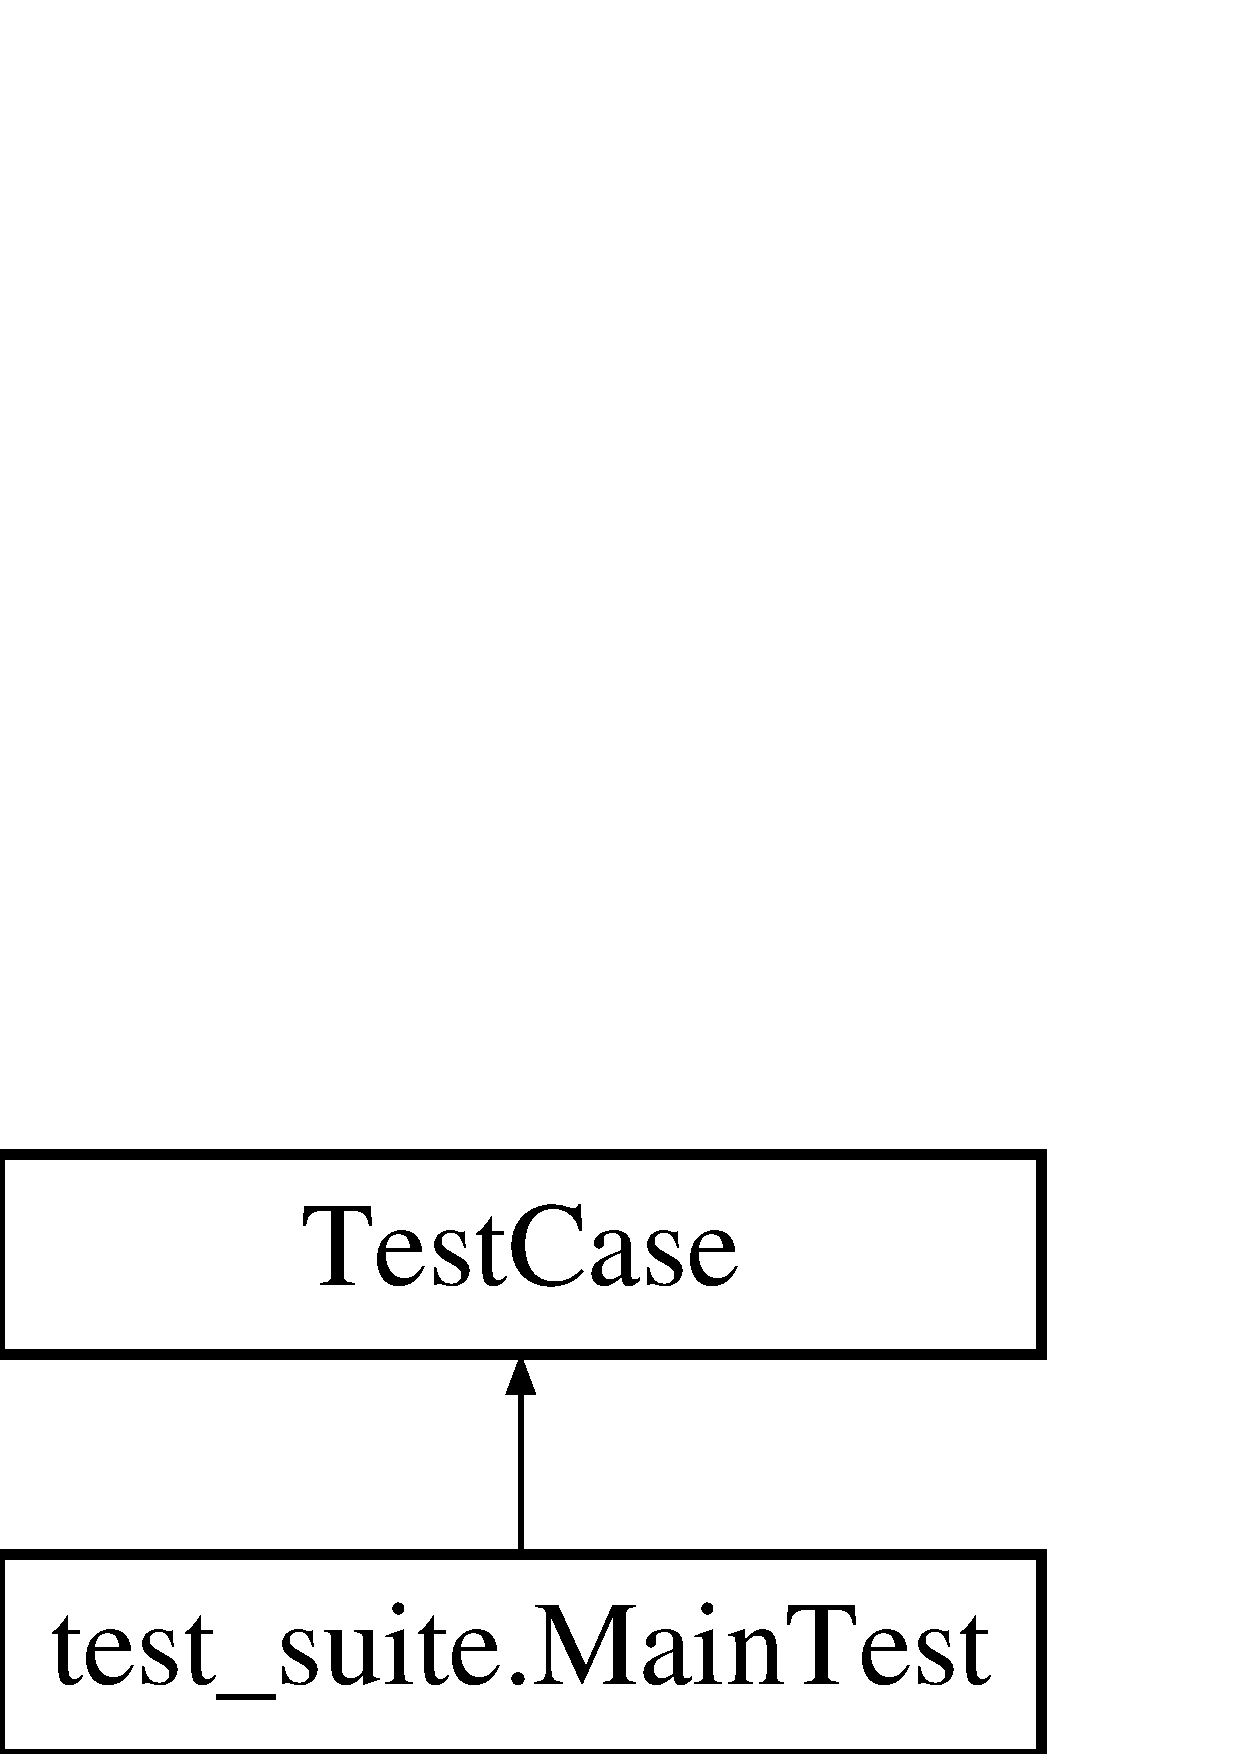
\includegraphics[height=2.000000cm]{classtest__suite_1_1MainTest}
\end{center}
\end{figure}
\subsection*{Public Member Functions}
\begin{DoxyCompactItemize}
\item 
\hypertarget{classtest__suite_1_1MainTest_a57bb1945a0545f0fa500dcc90c169582}{def {\bfseries set\-Up}}\label{classtest__suite_1_1MainTest_a57bb1945a0545f0fa500dcc90c169582}

\end{DoxyCompactItemize}
\subsection*{Public Attributes}
\begin{DoxyCompactItemize}
\item 
\hypertarget{classtest__suite_1_1MainTest_a2b8604f658425b346560313e53b5043e}{{\bfseries app}}\label{classtest__suite_1_1MainTest_a2b8604f658425b346560313e53b5043e}

\item 
\hypertarget{classtest__suite_1_1MainTest_a5507ff6888c48491ca3b1c97fb7bd505}{{\bfseries task\-\_\-bar}}\label{classtest__suite_1_1MainTest_a5507ff6888c48491ca3b1c97fb7bd505}

\end{DoxyCompactItemize}


\subsection{Detailed Description}
\begin{DoxyVerb}Test the main viewport object.
\end{DoxyVerb}
 

The documentation for this class was generated from the following file\-:\begin{DoxyCompactItemize}
\item 
docs/extensions/extension\-\_\-template/test\-\_\-suite.\-py\end{DoxyCompactItemize}

\hypertarget{classcommotion__client_1_1GUI_1_1main__window_1_1MainWindow}{\section{commotion\-\_\-client.\-G\-U\-I.\-main\-\_\-window.\-Main\-Window Class Reference}
\label{classcommotion__client_1_1GUI_1_1main__window_1_1MainWindow}\index{commotion\-\_\-client.\-G\-U\-I.\-main\-\_\-window.\-Main\-Window@{commotion\-\_\-client.\-G\-U\-I.\-main\-\_\-window.\-Main\-Window}}
}
Inheritance diagram for commotion\-\_\-client.\-G\-U\-I.\-main\-\_\-window.\-Main\-Window\-:\begin{figure}[H]
\begin{center}
\leavevmode
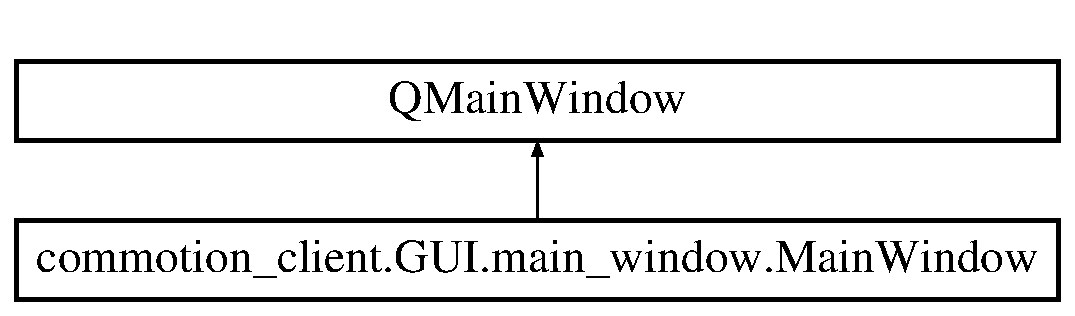
\includegraphics[height=2.000000cm]{classcommotion__client_1_1GUI_1_1main__window_1_1MainWindow}
\end{center}
\end{figure}
\subsection*{Public Member Functions}
\begin{DoxyCompactItemize}
\item 
\hypertarget{classcommotion__client_1_1GUI_1_1main__window_1_1MainWindow_a74b56753628f84bf3e19c128ef1fda19}{def {\bfseries \-\_\-\-\_\-init\-\_\-\-\_\-}}\label{classcommotion__client_1_1GUI_1_1main__window_1_1MainWindow_a74b56753628f84bf3e19c128ef1fda19}

\item 
\hypertarget{classcommotion__client_1_1GUI_1_1main__window_1_1MainWindow_a39b23e6f4f95af7d703ec03be942a7df}{def {\bfseries toggle\-\_\-menu\-\_\-bar}}\label{classcommotion__client_1_1GUI_1_1main__window_1_1MainWindow_a39b23e6f4f95af7d703ec03be942a7df}

\item 
def \hyperlink{classcommotion__client_1_1GUI_1_1main__window_1_1MainWindow_abacf45b62be7d880089c913e3f2f7f24}{setup\-\_\-menu\-\_\-bar}
\item 
def \hyperlink{classcommotion__client_1_1GUI_1_1main__window_1_1MainWindow_a2c803d1583ec7b548f5b2a9cb2014e4d}{init\-\_\-crash\-\_\-reporter}
\item 
def \hyperlink{classcommotion__client_1_1GUI_1_1main__window_1_1MainWindow_ad4d493c20e1d9898eeb41da87622ea49}{set\-\_\-viewport}
\item 
def \hyperlink{classcommotion__client_1_1GUI_1_1main__window_1_1MainWindow_a2972ac997218f50db2c18762ac48f23c}{apply\-\_\-viewport}
\item 
\hypertarget{classcommotion__client_1_1GUI_1_1main__window_1_1MainWindow_abf5e8a0add7f4fa1480c825a74e0e9b9}{def {\bfseries init\-\_\-viewport\-\_\-signals}}\label{classcommotion__client_1_1GUI_1_1main__window_1_1MainWindow_abf5e8a0add7f4fa1480c825a74e0e9b9}

\item 
def \hyperlink{classcommotion__client_1_1GUI_1_1main__window_1_1MainWindow_a0e9201cd1165369bdac93cf1b4658c6f}{change\-\_\-viewport}
\item 
def \hyperlink{classcommotion__client_1_1GUI_1_1main__window_1_1MainWindow_a08bdbda447c256d0cf5355d928ebb3fe}{init\-\_\-toolbar}
\item 
def \hyperlink{classcommotion__client_1_1GUI_1_1main__window_1_1MainWindow_a8e3325a8253a30ff8d900203d52a6e08}{purge}
\item 
def \hyperlink{classcommotion__client_1_1GUI_1_1main__window_1_1MainWindow_ac4b4245d881e0bd8417098bbf39e5353}{close\-Event}
\item 
def \hyperlink{classcommotion__client_1_1GUI_1_1main__window_1_1MainWindow_ab74365d561c1a4d58b9dc0932263f95e}{exit\-Event}
\item 
\hypertarget{classcommotion__client_1_1GUI_1_1main__window_1_1MainWindow_a73b785fffb64b1ce044326102b3727fe}{def {\bfseries cleanup}}\label{classcommotion__client_1_1GUI_1_1main__window_1_1MainWindow_a73b785fffb64b1ce044326102b3727fe}

\item 
def \hyperlink{classcommotion__client_1_1GUI_1_1main__window_1_1MainWindow_ab0859801750e4bae69f343539f0911f4}{bring\-\_\-front}
\item 
def \hyperlink{classcommotion__client_1_1GUI_1_1main__window_1_1MainWindow_a6f0d68762298dd620c75d8dbf48bb6c6}{load\-\_\-settings}
\item 
def \hyperlink{classcommotion__client_1_1GUI_1_1main__window_1_1MainWindow_aac10b214e6109d1e1beb63bf4795fc2c}{save\-\_\-settings}
\item 
def \hyperlink{classcommotion__client_1_1GUI_1_1main__window_1_1MainWindow_a418942bccd45d2282d3e8d094c2af812}{crash}
\item 
def \hyperlink{classcommotion__client_1_1GUI_1_1main__window_1_1MainWindow_a4a1d6ad4b512c85562374665160d0f81}{is\-\_\-dirty}
\end{DoxyCompactItemize}
\subsection*{Public Attributes}
\begin{DoxyCompactItemize}
\item 
\hypertarget{classcommotion__client_1_1GUI_1_1main__window_1_1MainWindow_a2023ddf9176abbc0419018bbdabdac2f}{{\bfseries log}}\label{classcommotion__client_1_1GUI_1_1main__window_1_1MainWindow_a2023ddf9176abbc0419018bbdabdac2f}

\item 
\hypertarget{classcommotion__client_1_1GUI_1_1main__window_1_1MainWindow_a60d2a4e45218021c9fbae2ed0bd6591e}{{\bfseries translate}}\label{classcommotion__client_1_1GUI_1_1main__window_1_1MainWindow_a60d2a4e45218021c9fbae2ed0bd6591e}

\item 
\hypertarget{classcommotion__client_1_1GUI_1_1main__window_1_1MainWindow_a5575e1a2084c7b32d0bb84062bba61d2}{{\bfseries ext\-\_\-manager}}\label{classcommotion__client_1_1GUI_1_1main__window_1_1MainWindow_a5575e1a2084c7b32d0bb84062bba61d2}

\item 
\hypertarget{classcommotion__client_1_1GUI_1_1main__window_1_1MainWindow_a7399ad8133834fe65dca400825f008e7}{{\bfseries viewport}}\label{classcommotion__client_1_1GUI_1_1main__window_1_1MainWindow_a7399ad8133834fe65dca400825f008e7}

\item 
\hypertarget{classcommotion__client_1_1GUI_1_1main__window_1_1MainWindow_a3847d89a04b3c67dea37dcde3302d179}{{\bfseries exit\-On\-Close}}\label{classcommotion__client_1_1GUI_1_1main__window_1_1MainWindow_a3847d89a04b3c67dea37dcde3302d179}

\item 
\hypertarget{classcommotion__client_1_1GUI_1_1main__window_1_1MainWindow_a7d944f7a540b8c7270e711d1f2e23f40}{{\bfseries remove\-\_\-on\-\_\-close}}\label{classcommotion__client_1_1GUI_1_1main__window_1_1MainWindow_a7d944f7a540b8c7270e711d1f2e23f40}

\item 
\hypertarget{classcommotion__client_1_1GUI_1_1main__window_1_1MainWindow_aeb2999af8c5674cefb026fdb70e72cea}{{\bfseries menu\-\_\-bar}}\label{classcommotion__client_1_1GUI_1_1main__window_1_1MainWindow_aeb2999af8c5674cefb026fdb70e72cea}

\item 
\hypertarget{classcommotion__client_1_1GUI_1_1main__window_1_1MainWindow_a94ece117d428ecf011a8a8a8d2bf6d14}{{\bfseries menu\-\_\-dock}}\label{classcommotion__client_1_1GUI_1_1main__window_1_1MainWindow_a94ece117d428ecf011a8a8a8d2bf6d14}

\item 
\hypertarget{classcommotion__client_1_1GUI_1_1main__window_1_1MainWindow_a8db26e620ef13fbbe69c8f148a34500a}{{\bfseries crash\-\_\-report}}\label{classcommotion__client_1_1GUI_1_1main__window_1_1MainWindow_a8db26e620ef13fbbe69c8f148a34500a}

\item 
\hypertarget{classcommotion__client_1_1GUI_1_1main__window_1_1MainWindow_a6f0f7b66344ea647e8bdf9c73c94a3a4}{{\bfseries central\-\_\-widget}}\label{classcommotion__client_1_1GUI_1_1main__window_1_1MainWindow_a6f0f7b66344ea647e8bdf9c73c94a3a4}

\item 
\hypertarget{classcommotion__client_1_1GUI_1_1main__window_1_1MainWindow_a8ca81a512a5d12b59a8804d7fc0f3cc4}{{\bfseries toolbar}}\label{classcommotion__client_1_1GUI_1_1main__window_1_1MainWindow_a8ca81a512a5d12b59a8804d7fc0f3cc4}

\item 
\hypertarget{classcommotion__client_1_1GUI_1_1main__window_1_1MainWindow_af8938670870bbbca1f3ddbd6c6f6dbc9}{{\bfseries scroll\-\_\-area}}\label{classcommotion__client_1_1GUI_1_1main__window_1_1MainWindow_af8938670870bbbca1f3ddbd6c6f6dbc9}

\item 
\hypertarget{classcommotion__client_1_1GUI_1_1main__window_1_1MainWindow_ab76561f5e9d503a6b8b206b34216456e}{{\bfseries next\-\_\-extension}}\label{classcommotion__client_1_1GUI_1_1main__window_1_1MainWindow_ab76561f5e9d503a6b8b206b34216456e}

\end{DoxyCompactItemize}
\subsection*{Static Public Attributes}
\begin{DoxyCompactItemize}
\item 
\hypertarget{classcommotion__client_1_1GUI_1_1main__window_1_1MainWindow_ab292f94c227c2991821b57613f7cc97e}{tuple {\bfseries clean\-\_\-up} = Qt\-Core.\-pyqt\-Signal()}\label{classcommotion__client_1_1GUI_1_1main__window_1_1MainWindow_ab292f94c227c2991821b57613f7cc97e}

\item 
\hypertarget{classcommotion__client_1_1GUI_1_1main__window_1_1MainWindow_afb5eded7d32749c78632fb2462e7baaf}{tuple {\bfseries app\-\_\-message} = Qt\-Core.\-pyqt\-Signal(str)}\label{classcommotion__client_1_1GUI_1_1main__window_1_1MainWindow_afb5eded7d32749c78632fb2462e7baaf}

\end{DoxyCompactItemize}


\subsection{Detailed Description}
\begin{DoxyVerb}The central widget for the commotion client. This widget initalizes all other sub-widgets and extensions as well as defines the paramiters of the main GUI container.
\end{DoxyVerb}
 

\subsection{Member Function Documentation}
\hypertarget{classcommotion__client_1_1GUI_1_1main__window_1_1MainWindow_a2972ac997218f50db2c18762ac48f23c}{\index{commotion\-\_\-client\-::\-G\-U\-I\-::main\-\_\-window\-::\-Main\-Window@{commotion\-\_\-client\-::\-G\-U\-I\-::main\-\_\-window\-::\-Main\-Window}!apply\-\_\-viewport@{apply\-\_\-viewport}}
\index{apply\-\_\-viewport@{apply\-\_\-viewport}!commotion_client::GUI::main_window::MainWindow@{commotion\-\_\-client\-::\-G\-U\-I\-::main\-\_\-window\-::\-Main\-Window}}
\subsubsection[{apply\-\_\-viewport}]{\setlength{\rightskip}{0pt plus 5cm}def commotion\-\_\-client.\-G\-U\-I.\-main\-\_\-window.\-Main\-Window.\-apply\-\_\-viewport (
\begin{DoxyParamCaption}
\item[{}]{self, }
\item[{}]{viewport, }
\item[{}]{toolbar = {\ttfamily None}}
\end{DoxyParamCaption}
)}}\label{classcommotion__client_1_1GUI_1_1main__window_1_1MainWindow_a2972ac997218f50db2c18762ac48f23c}
\begin{DoxyVerb}Apply current viewport to the central widget and set up proper signal's for communication. \end{DoxyVerb}
 

References commotion\-\_\-client.\-G\-U\-I.\-main\-\_\-window.\-Main\-Window.\-central\-\_\-widget, commotion\-\_\-client.\-G\-U\-I.\-main\-\_\-window.\-Main\-Window.\-init\-\_\-toolbar(), commotion\-\_\-client.\-G\-U\-I.\-main\-\_\-window.\-Main\-Window.\-init\-\_\-viewport\-\_\-signals(), commotion\-\_\-client.\-G\-U\-I.\-main\-\_\-window.\-Main\-Window.\-scroll\-\_\-area, commotion\-\_\-client.\-G\-U\-I.\-main\-\_\-window.\-Main\-Window.\-toolbar, commotion\-\_\-client.\-G\-U\-I.\-extension\-\_\-toolbar.\-Extension\-Tool\-Bar.\-viewport, commotion\-\_\-client.\-G\-U\-I.\-main\-\_\-window.\-Main\-Window.\-viewport, and commotion\-\_\-client.\-G\-U\-I.\-extension\-\_\-toolbar.\-Menu\-Item.\-viewport.



Referenced by commotion\-\_\-client.\-G\-U\-I.\-main\-\_\-window.\-Main\-Window.\-set\-\_\-viewport().


\begin{DoxyCode}
113 
114     \textcolor{keyword}{def }\hyperlink{classcommotion__client_1_1GUI_1_1main__window_1_1MainWindow_a2972ac997218f50db2c18762ac48f23c}{apply\_viewport}(self, viewport, toolbar=None):
115         \textcolor{stringliteral}{"""Apply current viewport to the central widget and set up proper signal's for communication. """}
116         \textcolor{comment}{#Create central widget (replaced due to splitter)}
117         \textcolor{comment}{#        self.central\_widget = QtGui.QWidget(self)}
118         self.\hyperlink{classcommotion__client_1_1GUI_1_1main__window_1_1MainWindow_a6f0f7b66344ea647e8bdf9c73c94a3a4}{central\_widget} = QtGui.QSplitter(QtCore.Qt.Vertical, self)
119         self.\hyperlink{classcommotion__client_1_1GUI_1_1main__window_1_1MainWindow_a7399ad8133834fe65dca400825f008e7}{viewport} = viewport(self.\hyperlink{classcommotion__client_1_1GUI_1_1main__window_1_1MainWindow_a6f0f7b66344ea647e8bdf9c73c94a3a4}{central\_widget})
120         \textcolor{keywordflow}{if} \textcolor{keywordflow}{not} toolbar:
121             toolbar = \textcolor{keyword}{False}
122         self.\hyperlink{classcommotion__client_1_1GUI_1_1main__window_1_1MainWindow_a8ca81a512a5d12b59a8804d7fc0f3cc4}{toolbar} = self.\hyperlink{classcommotion__client_1_1GUI_1_1main__window_1_1MainWindow_a08bdbda447c256d0cf5355d928ebb3fe}{init\_toolbar}(toolbar)
123 
124         \textcolor{comment}{#Set up central layout (Replaced due to splitter)}
125         \textcolor{comment}{#self.central\_layout = QtGui.QVBoxLayout(self.central\_widget)}
126 
127         self.\hyperlink{classcommotion__client_1_1GUI_1_1main__window_1_1MainWindow_af8938670870bbbca1f3ddbd6c6f6dbc9}{scroll\_area} = QtGui.QScrollArea(self.\hyperlink{classcommotion__client_1_1GUI_1_1main__window_1_1MainWindow_a6f0f7b66344ea647e8bdf9c73c94a3a4}{central\_widget})
128         self.scroll\_area.setWidgetResizable(\textcolor{keyword}{True})
129         self.scroll\_area.setWidget(self.\hyperlink{classcommotion__client_1_1GUI_1_1main__window_1_1MainWindow_a7399ad8133834fe65dca400825f008e7}{viewport})
130 
131         \textcolor{comment}{#add scroll area to central layout (replaced due to splitter)}
132         \textcolor{comment}{#self.central\_layout.addWidget(self.scroll\_area)}
133 
134         self.central\_widget.addWidget(self.\hyperlink{classcommotion__client_1_1GUI_1_1main__window_1_1MainWindow_af8938670870bbbca1f3ddbd6c6f6dbc9}{scroll\_area})
135         self.central\_widget.addWidget(self.\hyperlink{classcommotion__client_1_1GUI_1_1main__window_1_1MainWindow_a8ca81a512a5d12b59a8804d7fc0f3cc4}{toolbar})
136         
137         self.setCentralWidget(self.\hyperlink{classcommotion__client_1_1GUI_1_1main__window_1_1MainWindow_a6f0f7b66344ea647e8bdf9c73c94a3a4}{central\_widget})
138         self.\hyperlink{classcommotion__client_1_1GUI_1_1main__window_1_1MainWindow_abf5e8a0add7f4fa1480c825a74e0e9b9}{init\_viewport\_signals}()
139         self.central\_widget.show()
140         self.viewport.show()

\end{DoxyCode}
\hypertarget{classcommotion__client_1_1GUI_1_1main__window_1_1MainWindow_ab0859801750e4bae69f343539f0911f4}{\index{commotion\-\_\-client\-::\-G\-U\-I\-::main\-\_\-window\-::\-Main\-Window@{commotion\-\_\-client\-::\-G\-U\-I\-::main\-\_\-window\-::\-Main\-Window}!bring\-\_\-front@{bring\-\_\-front}}
\index{bring\-\_\-front@{bring\-\_\-front}!commotion_client::GUI::main_window::MainWindow@{commotion\-\_\-client\-::\-G\-U\-I\-::main\-\_\-window\-::\-Main\-Window}}
\subsubsection[{bring\-\_\-front}]{\setlength{\rightskip}{0pt plus 5cm}def commotion\-\_\-client.\-G\-U\-I.\-main\-\_\-window.\-Main\-Window.\-bring\-\_\-front (
\begin{DoxyParamCaption}
\item[{}]{self}
\end{DoxyParamCaption}
)}}\label{classcommotion__client_1_1GUI_1_1main__window_1_1MainWindow_ab0859801750e4bae69f343539f0911f4}
\begin{DoxyVerb}Brings the main window to the front of the screen.
\end{DoxyVerb}
 
\begin{DoxyCode}
209 
210     \textcolor{keyword}{def }\hyperlink{classcommotion__client_1_1GUI_1_1main__window_1_1MainWindow_ab0859801750e4bae69f343539f0911f4}{bring\_front}(self):
211         \textcolor{stringliteral}{"""}
212 \textcolor{stringliteral}{        Brings the main window to the front of the screen.}
213 \textcolor{stringliteral}{        """}
214         self.show()
215         self.raise\_()

\end{DoxyCode}
\hypertarget{classcommotion__client_1_1GUI_1_1main__window_1_1MainWindow_a0e9201cd1165369bdac93cf1b4658c6f}{\index{commotion\-\_\-client\-::\-G\-U\-I\-::main\-\_\-window\-::\-Main\-Window@{commotion\-\_\-client\-::\-G\-U\-I\-::main\-\_\-window\-::\-Main\-Window}!change\-\_\-viewport@{change\-\_\-viewport}}
\index{change\-\_\-viewport@{change\-\_\-viewport}!commotion_client::GUI::main_window::MainWindow@{commotion\-\_\-client\-::\-G\-U\-I\-::main\-\_\-window\-::\-Main\-Window}}
\subsubsection[{change\-\_\-viewport}]{\setlength{\rightskip}{0pt plus 5cm}def commotion\-\_\-client.\-G\-U\-I.\-main\-\_\-window.\-Main\-Window.\-change\-\_\-viewport (
\begin{DoxyParamCaption}
\item[{}]{self, }
\item[{}]{viewport}
\end{DoxyParamCaption}
)}}\label{classcommotion__client_1_1GUI_1_1main__window_1_1MainWindow_a0e9201cd1165369bdac93cf1b4658c6f}
\begin{DoxyVerb}Prepare next viewport for loading and start loading process when ready.\end{DoxyVerb}
 

References commotion\-\_\-client.\-G\-U\-I.\-main\-\_\-window.\-Main\-Window.\-next\-\_\-extension, commotion\-\_\-client.\-G\-U\-I.\-main\-\_\-window.\-Main\-Window.\-set\-\_\-viewport(), commotion\-\_\-client.\-extensions.\-config\-\_\-editor.\-main.\-View\-Port.\-translate, commotion\-\_\-client.\-G\-U\-I.\-main\-\_\-window.\-Main\-Window.\-translate, commotion\-\_\-client.\-G\-U\-I.\-extension\-\_\-toolbar.\-Extension\-Tool\-Bar.\-translate, commotion\-\_\-client.\-G\-U\-I.\-extension\-\_\-toolbar.\-Menu\-Item.\-translate, and commotion\-\_\-client.\-commotion\-\_\-client.\-Commotion\-Client\-Application.\-translate.


\begin{DoxyCode}
152 
153     \textcolor{keyword}{def }\hyperlink{classcommotion__client_1_1GUI_1_1main__window_1_1MainWindow_a0e9201cd1165369bdac93cf1b4658c6f}{change\_viewport}(self, viewport):
154         \textcolor{stringliteral}{"""Prepare next viewport for loading and start loading process when ready."""}
155         self.log.debug(self.\hyperlink{classcommotion__client_1_1GUI_1_1main__window_1_1MainWindow_a60d2a4e45218021c9fbae2ed0bd6591e}{translate}(\textcolor{stringliteral}{"logs"}, \textcolor{stringliteral}{"Request to change viewport received."}))
156         self.\hyperlink{classcommotion__client_1_1GUI_1_1main__window_1_1MainWindow_ab76561f5e9d503a6b8b206b34216456e}{next\_extension} = viewport
157         \textcolor{keywordflow}{if} self.viewport.is\_dirty:
158             self.viewport.on\_stop.connect(self.\hyperlink{classcommotion__client_1_1GUI_1_1main__window_1_1MainWindow_ad4d493c20e1d9898eeb41da87622ea49}{set\_viewport})
159             self.clean\_up.emit()
160         \textcolor{keywordflow}{else}:
161             self.\hyperlink{classcommotion__client_1_1GUI_1_1main__window_1_1MainWindow_ad4d493c20e1d9898eeb41da87622ea49}{set\_viewport}()

\end{DoxyCode}
\hypertarget{classcommotion__client_1_1GUI_1_1main__window_1_1MainWindow_ac4b4245d881e0bd8417098bbf39e5353}{\index{commotion\-\_\-client\-::\-G\-U\-I\-::main\-\_\-window\-::\-Main\-Window@{commotion\-\_\-client\-::\-G\-U\-I\-::main\-\_\-window\-::\-Main\-Window}!close\-Event@{close\-Event}}
\index{close\-Event@{close\-Event}!commotion_client::GUI::main_window::MainWindow@{commotion\-\_\-client\-::\-G\-U\-I\-::main\-\_\-window\-::\-Main\-Window}}
\subsubsection[{close\-Event}]{\setlength{\rightskip}{0pt plus 5cm}def commotion\-\_\-client.\-G\-U\-I.\-main\-\_\-window.\-Main\-Window.\-close\-Event (
\begin{DoxyParamCaption}
\item[{}]{self, }
\item[{}]{event}
\end{DoxyParamCaption}
)}}\label{classcommotion__client_1_1GUI_1_1main__window_1_1MainWindow_ac4b4245d881e0bd8417098bbf39e5353}
\begin{DoxyVerb}Captures the close event for the main window. When called from exitEvent removes a trayIcon and accepts its demise. When called otherwise will simply hide the main window and ignore the event.
\end{DoxyVerb}
 

References commotion\-\_\-client.\-G\-U\-I.\-main\-\_\-window.\-Main\-Window.\-exit\-On\-Close, commotion\-\_\-client.\-G\-U\-I.\-main\-\_\-window.\-Main\-Window.\-remove\-\_\-on\-\_\-close, commotion\-\_\-client.\-extensions.\-config\-\_\-editor.\-main.\-View\-Port.\-translate, commotion\-\_\-client.\-G\-U\-I.\-main\-\_\-window.\-Main\-Window.\-translate, commotion\-\_\-client.\-G\-U\-I.\-extension\-\_\-toolbar.\-Extension\-Tool\-Bar.\-translate, commotion\-\_\-client.\-G\-U\-I.\-extension\-\_\-toolbar.\-Menu\-Item.\-translate, and commotion\-\_\-client.\-commotion\-\_\-client.\-Commotion\-Client\-Application.\-translate.


\begin{DoxyCode}
177 
178     \textcolor{keyword}{def }\hyperlink{classcommotion__client_1_1GUI_1_1main__window_1_1MainWindow_ac4b4245d881e0bd8417098bbf39e5353}{closeEvent}(self, event):
179         \textcolor{stringliteral}{"""}
180 \textcolor{stringliteral}{        Captures the close event for the main window. When called from exitEvent removes a trayIcon and
       accepts its demise. When called otherwise will simply hide the main window and ignore the event.}
181 \textcolor{stringliteral}{        """}
182         
183         \textcolor{keywordflow}{if} self.\hyperlink{classcommotion__client_1_1GUI_1_1main__window_1_1MainWindow_a3847d89a04b3c67dea37dcde3302d179}{exitOnClose}:
184             self.log.debug(self.\hyperlink{classcommotion__client_1_1GUI_1_1main__window_1_1MainWindow_a60d2a4e45218021c9fbae2ed0bd6591e}{translate}(\textcolor{stringliteral}{"logs"}, \textcolor{stringliteral}{"Application has received a EXIT close event and
       will shutdown completely."}))
185             event.accept()
186         \textcolor{keywordflow}{elif} self.\hyperlink{classcommotion__client_1_1GUI_1_1main__window_1_1MainWindow_a7d944f7a540b8c7270e711d1f2e23f40}{remove\_on\_close}:
187             self.log.debug(self.\hyperlink{classcommotion__client_1_1GUI_1_1main__window_1_1MainWindow_a60d2a4e45218021c9fbae2ed0bd6591e}{translate}(\textcolor{stringliteral}{"logs"}, \textcolor{stringliteral}{"Application has received a GUI closing close
       event and will close its main window."}))
188             self.deleteLater()
189             event.accept()
190         \textcolor{keywordflow}{else}:
191             self.log.debug(self.\hyperlink{classcommotion__client_1_1GUI_1_1main__window_1_1MainWindow_a60d2a4e45218021c9fbae2ed0bd6591e}{translate}(\textcolor{stringliteral}{"logs"}, \textcolor{stringliteral}{"Application has received a non-exit close event
       and will hide its main window."}))
192             self.hide()
193             event.setAccepted(\textcolor{keyword}{True})
194             event.ignore()

\end{DoxyCode}
\hypertarget{classcommotion__client_1_1GUI_1_1main__window_1_1MainWindow_a418942bccd45d2282d3e8d094c2af812}{\index{commotion\-\_\-client\-::\-G\-U\-I\-::main\-\_\-window\-::\-Main\-Window@{commotion\-\_\-client\-::\-G\-U\-I\-::main\-\_\-window\-::\-Main\-Window}!crash@{crash}}
\index{crash@{crash}!commotion_client::GUI::main_window::MainWindow@{commotion\-\_\-client\-::\-G\-U\-I\-::main\-\_\-window\-::\-Main\-Window}}
\subsubsection[{crash}]{\setlength{\rightskip}{0pt plus 5cm}def commotion\-\_\-client.\-G\-U\-I.\-main\-\_\-window.\-Main\-Window.\-crash (
\begin{DoxyParamCaption}
\item[{}]{self, }
\item[{}]{crash\-\_\-type}
\end{DoxyParamCaption}
)}}\label{classcommotion__client_1_1GUI_1_1main__window_1_1MainWindow_a418942bccd45d2282d3e8d094c2af812}
\begin{DoxyVerb}Emits a closing signal to allow other windows who need to clean up to clean up and then exits the application.
\end{DoxyVerb}
 

References commotion\-\_\-client.\-G\-U\-I.\-main\-\_\-window.\-Main\-Window.\-exit\-On\-Close.



Referenced by commotion\-\_\-client.\-G\-U\-I.\-main\-\_\-window.\-Main\-Window.\-init\-\_\-crash\-\_\-reporter().


\begin{DoxyCode}
253 
254     \textcolor{keyword}{def }\hyperlink{classcommotion__client_1_1GUI_1_1main__window_1_1MainWindow_a418942bccd45d2282d3e8d094c2af812}{crash}(self, crash\_type):
255         \textcolor{stringliteral}{"""}
256 \textcolor{stringliteral}{        Emits a closing signal to allow other windows who need to clean up to clean up and then exits the
       application.}
257 \textcolor{stringliteral}{        """}
258         self.clean\_up.emit() \textcolor{comment}{#send signal for others to clean up if they need to}
259         \textcolor{keywordflow}{if} crash\_type == \textcolor{stringliteral}{"restart"}:
260             self.app\_message.emit(\textcolor{stringliteral}{"restart"})
261         \textcolor{keywordflow}{else}:
262             self.\hyperlink{classcommotion__client_1_1GUI_1_1main__window_1_1MainWindow_a3847d89a04b3c67dea37dcde3302d179}{exitOnClose} = \textcolor{keyword}{True}
263             self.close()
            
\end{DoxyCode}
\hypertarget{classcommotion__client_1_1GUI_1_1main__window_1_1MainWindow_ab74365d561c1a4d58b9dc0932263f95e}{\index{commotion\-\_\-client\-::\-G\-U\-I\-::main\-\_\-window\-::\-Main\-Window@{commotion\-\_\-client\-::\-G\-U\-I\-::main\-\_\-window\-::\-Main\-Window}!exit\-Event@{exit\-Event}}
\index{exit\-Event@{exit\-Event}!commotion_client::GUI::main_window::MainWindow@{commotion\-\_\-client\-::\-G\-U\-I\-::main\-\_\-window\-::\-Main\-Window}}
\subsubsection[{exit\-Event}]{\setlength{\rightskip}{0pt plus 5cm}def commotion\-\_\-client.\-G\-U\-I.\-main\-\_\-window.\-Main\-Window.\-exit\-Event (
\begin{DoxyParamCaption}
\item[{}]{self}
\end{DoxyParamCaption}
)}}\label{classcommotion__client_1_1GUI_1_1main__window_1_1MainWindow_ab74365d561c1a4d58b9dc0932263f95e}
\begin{DoxyVerb}Closes and exits the entire commotion program.
\end{DoxyVerb}
 

References commotion\-\_\-client.\-G\-U\-I.\-main\-\_\-window.\-Main\-Window.\-cleanup(), commotion\-\_\-client.\-G\-U\-I.\-main\-\_\-window.\-Main\-Window.\-exit\-On\-Close, commotion\-\_\-client.\-extensions.\-config\-\_\-editor.\-main.\-View\-Port.\-is\-\_\-dirty(), commotion\-\_\-client.\-G\-U\-I.\-main\-\_\-window.\-Main\-Window.\-is\-\_\-dirty(), and commotion\-\_\-client.\-G\-U\-I.\-main\-\_\-window.\-Main\-Window.\-save\-\_\-settings().


\begin{DoxyCode}
195 
196     \textcolor{keyword}{def }\hyperlink{classcommotion__client_1_1GUI_1_1main__window_1_1MainWindow_ab74365d561c1a4d58b9dc0932263f95e}{exitEvent}(self):
197         \textcolor{stringliteral}{"""}
198 \textcolor{stringliteral}{        Closes and exits the entire commotion program.}
199 \textcolor{stringliteral}{        """}
200         self.\hyperlink{classcommotion__client_1_1GUI_1_1main__window_1_1MainWindow_a73b785fffb64b1ce044326102b3727fe}{cleanup}()
201         self.\hyperlink{classcommotion__client_1_1GUI_1_1main__window_1_1MainWindow_a3847d89a04b3c67dea37dcde3302d179}{exitOnClose} = \textcolor{keyword}{True}
202         self.close()

\end{DoxyCode}
\hypertarget{classcommotion__client_1_1GUI_1_1main__window_1_1MainWindow_a2c803d1583ec7b548f5b2a9cb2014e4d}{\index{commotion\-\_\-client\-::\-G\-U\-I\-::main\-\_\-window\-::\-Main\-Window@{commotion\-\_\-client\-::\-G\-U\-I\-::main\-\_\-window\-::\-Main\-Window}!init\-\_\-crash\-\_\-reporter@{init\-\_\-crash\-\_\-reporter}}
\index{init\-\_\-crash\-\_\-reporter@{init\-\_\-crash\-\_\-reporter}!commotion_client::GUI::main_window::MainWindow@{commotion\-\_\-client\-::\-G\-U\-I\-::main\-\_\-window\-::\-Main\-Window}}
\subsubsection[{init\-\_\-crash\-\_\-reporter}]{\setlength{\rightskip}{0pt plus 5cm}def commotion\-\_\-client.\-G\-U\-I.\-main\-\_\-window.\-Main\-Window.\-init\-\_\-crash\-\_\-reporter (
\begin{DoxyParamCaption}
\item[{}]{self}
\end{DoxyParamCaption}
)}}\label{classcommotion__client_1_1GUI_1_1main__window_1_1MainWindow_a2c803d1583ec7b548f5b2a9cb2014e4d}
\begin{DoxyVerb}\end{DoxyVerb}
 

References commotion\-\_\-client.\-G\-U\-I.\-crash\-\_\-report.\-Crash\-Report.\-crash, commotion\-\_\-client.\-G\-U\-I.\-main\-\_\-window.\-Main\-Window.\-crash(), commotion\-\_\-client.\-G\-U\-I.\-main\-\_\-window.\-Main\-Window.\-crash\-\_\-report, commotion\-\_\-client.\-extensions.\-config\-\_\-editor.\-main.\-View\-Port.\-translate, commotion\-\_\-client.\-G\-U\-I.\-main\-\_\-window.\-Main\-Window.\-translate, commotion\-\_\-client.\-G\-U\-I.\-extension\-\_\-toolbar.\-Extension\-Tool\-Bar.\-translate, commotion\-\_\-client.\-G\-U\-I.\-extension\-\_\-toolbar.\-Menu\-Item.\-translate, and commotion\-\_\-client.\-commotion\-\_\-client.\-Commotion\-Client\-Application.\-translate.


\begin{DoxyCode}
94 
95     \textcolor{keyword}{def }\hyperlink{classcommotion__client_1_1GUI_1_1main__window_1_1MainWindow_a2c803d1583ec7b548f5b2a9cb2014e4d}{init\_crash\_reporter}(self):
96         \textcolor{stringliteral}{""" """}
97         \textcolor{keywordflow}{try}:
98             self.\hyperlink{classcommotion__client_1_1GUI_1_1main__window_1_1MainWindow_a8db26e620ef13fbbe69c8f148a34500a}{crash\_report} = \hyperlink{classcommotion__client_1_1GUI_1_1crash__report_1_1CrashReport}{CrashReport}()
99         \textcolor{keywordflow}{except} Exception \textcolor{keyword}{as} \_excp:
100             self.log.critical(self.\hyperlink{classcommotion__client_1_1GUI_1_1main__window_1_1MainWindow_a60d2a4e45218021c9fbae2ed0bd6591e}{translate}(\textcolor{stringliteral}{"logs"}, \textcolor{stringliteral}{"Failed to load crash reporter. Ironically,
       this means that the application must be halted."}))
101             self.log.exception(\_excp)
102             \textcolor{keywordflow}{raise}
103         \textcolor{keywordflow}{else}:
104             self.crash\_report.crash.connect(self.\hyperlink{classcommotion__client_1_1GUI_1_1main__window_1_1MainWindow_a418942bccd45d2282d3e8d094c2af812}{crash})

\end{DoxyCode}
\hypertarget{classcommotion__client_1_1GUI_1_1main__window_1_1MainWindow_a08bdbda447c256d0cf5355d928ebb3fe}{\index{commotion\-\_\-client\-::\-G\-U\-I\-::main\-\_\-window\-::\-Main\-Window@{commotion\-\_\-client\-::\-G\-U\-I\-::main\-\_\-window\-::\-Main\-Window}!init\-\_\-toolbar@{init\-\_\-toolbar}}
\index{init\-\_\-toolbar@{init\-\_\-toolbar}!commotion_client::GUI::main_window::MainWindow@{commotion\-\_\-client\-::\-G\-U\-I\-::main\-\_\-window\-::\-Main\-Window}}
\subsubsection[{init\-\_\-toolbar}]{\setlength{\rightskip}{0pt plus 5cm}def commotion\-\_\-client.\-G\-U\-I.\-main\-\_\-window.\-Main\-Window.\-init\-\_\-toolbar (
\begin{DoxyParamCaption}
\item[{}]{self, }
\item[{}]{ext\-\_\-toolbar}
\end{DoxyParamCaption}
)}}\label{classcommotion__client_1_1GUI_1_1main__window_1_1MainWindow_a08bdbda447c256d0cf5355d928ebb3fe}
\begin{DoxyVerb}\end{DoxyVerb}
 

References commotion\-\_\-client.\-G\-U\-I.\-main\-\_\-window.\-Main\-Window.\-central\-\_\-widget, commotion\-\_\-client.\-G\-U\-I.\-extension\-\_\-toolbar.\-Extension\-Tool\-Bar.\-viewport, commotion\-\_\-client.\-G\-U\-I.\-main\-\_\-window.\-Main\-Window.\-viewport, and commotion\-\_\-client.\-G\-U\-I.\-extension\-\_\-toolbar.\-Menu\-Item.\-viewport.



Referenced by commotion\-\_\-client.\-G\-U\-I.\-main\-\_\-window.\-Main\-Window.\-apply\-\_\-viewport().


\begin{DoxyCode}
162 
163     \textcolor{keyword}{def }\hyperlink{classcommotion__client_1_1GUI_1_1main__window_1_1MainWindow_a08bdbda447c256d0cf5355d928ebb3fe}{init\_toolbar}(self, ext\_toolbar):
164         \textcolor{stringliteral}{""" """}
165         toolbar = \hyperlink{classcommotion__client_1_1GUI_1_1toolbar__builder_1_1ToolBar}{toolbar\_builder.ToolBar}(self.
      \hyperlink{classcommotion__client_1_1GUI_1_1main__window_1_1MainWindow_a6f0f7b66344ea647e8bdf9c73c94a3a4}{central\_widget},  self.\hyperlink{classcommotion__client_1_1GUI_1_1main__window_1_1MainWindow_a7399ad8133834fe65dca400825f008e7}{viewport}, ext\_toolbar,)
166         \textcolor{keywordflow}{return} toolbar
167         
            
\end{DoxyCode}
\hypertarget{classcommotion__client_1_1GUI_1_1main__window_1_1MainWindow_a4a1d6ad4b512c85562374665160d0f81}{\index{commotion\-\_\-client\-::\-G\-U\-I\-::main\-\_\-window\-::\-Main\-Window@{commotion\-\_\-client\-::\-G\-U\-I\-::main\-\_\-window\-::\-Main\-Window}!is\-\_\-dirty@{is\-\_\-dirty}}
\index{is\-\_\-dirty@{is\-\_\-dirty}!commotion_client::GUI::main_window::MainWindow@{commotion\-\_\-client\-::\-G\-U\-I\-::main\-\_\-window\-::\-Main\-Window}}
\subsubsection[{is\-\_\-dirty}]{\setlength{\rightskip}{0pt plus 5cm}def commotion\-\_\-client.\-G\-U\-I.\-main\-\_\-window.\-Main\-Window.\-is\-\_\-dirty (
\begin{DoxyParamCaption}
\item[{}]{self}
\end{DoxyParamCaption}
)}}\label{classcommotion__client_1_1GUI_1_1main__window_1_1MainWindow_a4a1d6ad4b512c85562374665160d0f81}
\begin{DoxyVerb}Get the current state of the main window\end{DoxyVerb}
 

References commotion\-\_\-client.\-G\-U\-I.\-main\-\_\-window.\-Main\-Window.\-\_\-dirty, commotion\-\_\-client.\-G\-U\-I.\-extension\-\_\-toolbar.\-Extension\-Tool\-Bar.\-\_\-dirty, commotion\-\_\-client.\-extensions.\-config\-\_\-editor.\-main.\-View\-Port.\-\_\-dirty, and commotion\-\_\-client.\-G\-U\-I.\-extension\-\_\-toolbar.\-Menu\-Item.\-\_\-dirty.



Referenced by commotion\-\_\-client.\-G\-U\-I.\-main\-\_\-window.\-Main\-Window.\-exit\-Event().


\begin{DoxyCode}
265 
266     \textcolor{keyword}{def }\hyperlink{classcommotion__client_1_1GUI_1_1main__window_1_1MainWindow_a4a1d6ad4b512c85562374665160d0f81}{is\_dirty}(self):
267         \textcolor{stringliteral}{"""Get the current state of the main window"""}
268         \textcolor{keywordflow}{return} self.\hyperlink{classcommotion__client_1_1GUI_1_1main__window_1_1MainWindow_a77ea590cc2141219ae5041565301c49c}{\_dirty}
269 
270         
\end{DoxyCode}
\hypertarget{classcommotion__client_1_1GUI_1_1main__window_1_1MainWindow_a6f0d68762298dd620c75d8dbf48bb6c6}{\index{commotion\-\_\-client\-::\-G\-U\-I\-::main\-\_\-window\-::\-Main\-Window@{commotion\-\_\-client\-::\-G\-U\-I\-::main\-\_\-window\-::\-Main\-Window}!load\-\_\-settings@{load\-\_\-settings}}
\index{load\-\_\-settings@{load\-\_\-settings}!commotion_client::GUI::main_window::MainWindow@{commotion\-\_\-client\-::\-G\-U\-I\-::main\-\_\-window\-::\-Main\-Window}}
\subsubsection[{load\-\_\-settings}]{\setlength{\rightskip}{0pt plus 5cm}def commotion\-\_\-client.\-G\-U\-I.\-main\-\_\-window.\-Main\-Window.\-load\-\_\-settings (
\begin{DoxyParamCaption}
\item[{}]{self}
\end{DoxyParamCaption}
)}}\label{classcommotion__client_1_1GUI_1_1main__window_1_1MainWindow_a6f0d68762298dd620c75d8dbf48bb6c6}
\begin{DoxyVerb}Loads window geometry from saved settings and sets window to those settings.
\end{DoxyVerb}
 

References commotion\-\_\-client.\-extensions.\-config\-\_\-editor.\-main.\-View\-Port.\-translate, commotion\-\_\-client.\-G\-U\-I.\-main\-\_\-window.\-Main\-Window.\-translate, commotion\-\_\-client.\-G\-U\-I.\-extension\-\_\-toolbar.\-Extension\-Tool\-Bar.\-translate, commotion\-\_\-client.\-G\-U\-I.\-extension\-\_\-toolbar.\-Menu\-Item.\-translate, and commotion\-\_\-client.\-commotion\-\_\-client.\-Commotion\-Client\-Application.\-translate.



Referenced by commotion\-\_\-client.\-G\-U\-I.\-toolbar.\-Tool\-Bar.\-init\-\_\-settings(), and commotion\-\_\-client.\-G\-U\-I.\-toolbar\-\_\-builder.\-Tool\-Bar.\-init\-\_\-settings().


\begin{DoxyCode}
216 
217     \textcolor{keyword}{def }\hyperlink{classcommotion__client_1_1GUI_1_1main__window_1_1MainWindow_a6f0d68762298dd620c75d8dbf48bb6c6}{load\_settings}(self):
218         \textcolor{stringliteral}{"""}
219 \textcolor{stringliteral}{        Loads window geometry from saved settings and sets window to those settings.}
220 \textcolor{stringliteral}{        """}
221         defaults = \{
222             \textcolor{comment}{#QRect(posX, posY, width, height)}
223             \textcolor{stringliteral}{"geometry"}:QtCore.QRect(300, 300, 640, 480), \textcolor{comment}{#TODO set sane defaults and catalogue in HIG}
224         \}
225 
226         \_settings = QtCore.QSettings()
227         \_settings.beginGroup(\textcolor{stringliteral}{"MainWindow"})
228 
229         \textcolor{comment}{#Load settings from saved, or use defaults}
230         geometry = \_settings.value(\textcolor{stringliteral}{"geometry"}, defaults[\textcolor{stringliteral}{'geometry'}])
231         \textcolor{keywordflow}{if} geometry.isNull() == \textcolor{keyword}{True}:
232             \_error = self.\hyperlink{classcommotion__client_1_1GUI_1_1main__window_1_1MainWindow_a60d2a4e45218021c9fbae2ed0bd6591e}{translate}(\textcolor{stringliteral}{"logs"}, \textcolor{stringliteral}{"Could not load window geometry from settings file or
       defaults."})
233             self.log.critical(\_error)
234             \textcolor{keywordflow}{raise} EnvironmentError(\_error)
235         \_settings.endGroup()
236         self.setGeometry(geometry)

\end{DoxyCode}
\hypertarget{classcommotion__client_1_1GUI_1_1main__window_1_1MainWindow_a8e3325a8253a30ff8d900203d52a6e08}{\index{commotion\-\_\-client\-::\-G\-U\-I\-::main\-\_\-window\-::\-Main\-Window@{commotion\-\_\-client\-::\-G\-U\-I\-::main\-\_\-window\-::\-Main\-Window}!purge@{purge}}
\index{purge@{purge}!commotion_client::GUI::main_window::MainWindow@{commotion\-\_\-client\-::\-G\-U\-I\-::main\-\_\-window\-::\-Main\-Window}}
\subsubsection[{purge}]{\setlength{\rightskip}{0pt plus 5cm}def commotion\-\_\-client.\-G\-U\-I.\-main\-\_\-window.\-Main\-Window.\-purge (
\begin{DoxyParamCaption}
\item[{}]{self}
\end{DoxyParamCaption}
)}}\label{classcommotion__client_1_1GUI_1_1main__window_1_1MainWindow_a8e3325a8253a30ff8d900203d52a6e08}
\begin{DoxyVerb}Closes the menu and sets its data up for immediate removal.
\end{DoxyVerb}
 

References commotion\-\_\-client.\-G\-U\-I.\-main\-\_\-window.\-Main\-Window.\-cleanup().


\begin{DoxyCode}
168 
169     \textcolor{keyword}{def }\hyperlink{classcommotion__client_1_1GUI_1_1main__window_1_1MainWindow_a8e3325a8253a30ff8d900203d52a6e08}{purge}(self):
170         \textcolor{stringliteral}{"""}
171 \textcolor{stringliteral}{        Closes the menu and sets its data up for immediate removal.}
172 \textcolor{stringliteral}{        """}
173         self.\hyperlink{classcommotion__client_1_1GUI_1_1main__window_1_1MainWindow_a73b785fffb64b1ce044326102b3727fe}{cleanup}()
174         self.main.remove\_on\_close = \textcolor{keyword}{True}
175         self.close()
176 

\end{DoxyCode}
\hypertarget{classcommotion__client_1_1GUI_1_1main__window_1_1MainWindow_aac10b214e6109d1e1beb63bf4795fc2c}{\index{commotion\-\_\-client\-::\-G\-U\-I\-::main\-\_\-window\-::\-Main\-Window@{commotion\-\_\-client\-::\-G\-U\-I\-::main\-\_\-window\-::\-Main\-Window}!save\-\_\-settings@{save\-\_\-settings}}
\index{save\-\_\-settings@{save\-\_\-settings}!commotion_client::GUI::main_window::MainWindow@{commotion\-\_\-client\-::\-G\-U\-I\-::main\-\_\-window\-::\-Main\-Window}}
\subsubsection[{save\-\_\-settings}]{\setlength{\rightskip}{0pt plus 5cm}def commotion\-\_\-client.\-G\-U\-I.\-main\-\_\-window.\-Main\-Window.\-save\-\_\-settings (
\begin{DoxyParamCaption}
\item[{}]{self}
\end{DoxyParamCaption}
)}}\label{classcommotion__client_1_1GUI_1_1main__window_1_1MainWindow_aac10b214e6109d1e1beb63bf4795fc2c}
\begin{DoxyVerb}Saves current window geometry
\end{DoxyVerb}
 

References commotion\-\_\-client.\-extensions.\-config\-\_\-editor.\-main.\-View\-Port.\-translate, commotion\-\_\-client.\-G\-U\-I.\-main\-\_\-window.\-Main\-Window.\-translate, commotion\-\_\-client.\-G\-U\-I.\-extension\-\_\-toolbar.\-Extension\-Tool\-Bar.\-translate, commotion\-\_\-client.\-G\-U\-I.\-extension\-\_\-toolbar.\-Menu\-Item.\-translate, and commotion\-\_\-client.\-commotion\-\_\-client.\-Commotion\-Client\-Application.\-translate.



Referenced by commotion\-\_\-client.\-G\-U\-I.\-main\-\_\-window.\-Main\-Window.\-exit\-Event(), and commotion\-\_\-client.\-utils.\-extension\-\_\-manager.\-Extension\-Manager.\-install\-\_\-loaded().


\begin{DoxyCode}
237 
238     \textcolor{keyword}{def }\hyperlink{classcommotion__client_1_1GUI_1_1main__window_1_1MainWindow_aac10b214e6109d1e1beb63bf4795fc2c}{save\_settings}(self):
239         \textcolor{stringliteral}{"""}
240 \textcolor{stringliteral}{        Saves current window geometry}
241 \textcolor{stringliteral}{        """}
242 
243         \_settings = QtCore.QSettings()
244         \_settings.beginGroup(\textcolor{stringliteral}{"MainWindow"})
245         \textcolor{comment}{#Save settings}
246         \textcolor{keywordflow}{try}:
247             \_settings.setValue(\textcolor{stringliteral}{"geometry"}, self.geometry())
248         \textcolor{keywordflow}{except} Exception \textcolor{keyword}{as} \_excp:
249             self.log.warn(self.\hyperlink{classcommotion__client_1_1GUI_1_1main__window_1_1MainWindow_a60d2a4e45218021c9fbae2ed0bd6591e}{translate}(\textcolor{stringliteral}{"logs"}, \textcolor{stringliteral}{"Could not save window geometry. Will continue
       without saving window geometry."}))
250             self.log.exception(\_excp)
251         \_settings.endGroup()
252         

\end{DoxyCode}
\hypertarget{classcommotion__client_1_1GUI_1_1main__window_1_1MainWindow_ad4d493c20e1d9898eeb41da87622ea49}{\index{commotion\-\_\-client\-::\-G\-U\-I\-::main\-\_\-window\-::\-Main\-Window@{commotion\-\_\-client\-::\-G\-U\-I\-::main\-\_\-window\-::\-Main\-Window}!set\-\_\-viewport@{set\-\_\-viewport}}
\index{set\-\_\-viewport@{set\-\_\-viewport}!commotion_client::GUI::main_window::MainWindow@{commotion\-\_\-client\-::\-G\-U\-I\-::main\-\_\-window\-::\-Main\-Window}}
\subsubsection[{set\-\_\-viewport}]{\setlength{\rightskip}{0pt plus 5cm}def commotion\-\_\-client.\-G\-U\-I.\-main\-\_\-window.\-Main\-Window.\-set\-\_\-viewport (
\begin{DoxyParamCaption}
\item[{}]{self}
\end{DoxyParamCaption}
)}}\label{classcommotion__client_1_1GUI_1_1main__window_1_1MainWindow_ad4d493c20e1d9898eeb41da87622ea49}
\begin{DoxyVerb}Load and set viewport to next viewport and load viewport \end{DoxyVerb}
 

References commotion\-\_\-client.\-G\-U\-I.\-main\-\_\-window.\-Main\-Window.\-apply\-\_\-viewport(), and commotion\-\_\-client.\-G\-U\-I.\-main\-\_\-window.\-Main\-Window.\-next\-\_\-extension.



Referenced by commotion\-\_\-client.\-G\-U\-I.\-main\-\_\-window.\-Main\-Window.\-change\-\_\-viewport().


\begin{DoxyCode}
105 
106     \textcolor{keyword}{def }\hyperlink{classcommotion__client_1_1GUI_1_1main__window_1_1MainWindow_ad4d493c20e1d9898eeb41da87622ea49}{set\_viewport}(self):
107         \textcolor{stringliteral}{"""Load and set viewport to next viewport and load viewport """}
108         self.log.info(self.\hyperlink{classcommotion__client_1_1GUI_1_1main__window_1_1MainWindow_ab76561f5e9d503a6b8b206b34216456e}{next\_extension})
109         next\_view = self.\hyperlink{classcommotion__client_1_1GUI_1_1main__window_1_1MainWindow_ab76561f5e9d503a6b8b206b34216456e}{next\_extension}
110         ext\_viewport = self.ext\_manager.load\_user\_interface(str(next\_view), \textcolor{stringliteral}{"main"})
111         ext\_toolbar = self.ext\_manager.load\_user\_interface(str(next\_view), \textcolor{stringliteral}{"toolbar"})
112         self.\hyperlink{classcommotion__client_1_1GUI_1_1main__window_1_1MainWindow_a2972ac997218f50db2c18762ac48f23c}{apply\_viewport}(ext\_viewport, ext\_toolbar)
        
\end{DoxyCode}
\hypertarget{classcommotion__client_1_1GUI_1_1main__window_1_1MainWindow_abacf45b62be7d880089c913e3f2f7f24}{\index{commotion\-\_\-client\-::\-G\-U\-I\-::main\-\_\-window\-::\-Main\-Window@{commotion\-\_\-client\-::\-G\-U\-I\-::main\-\_\-window\-::\-Main\-Window}!setup\-\_\-menu\-\_\-bar@{setup\-\_\-menu\-\_\-bar}}
\index{setup\-\_\-menu\-\_\-bar@{setup\-\_\-menu\-\_\-bar}!commotion_client::GUI::main_window::MainWindow@{commotion\-\_\-client\-::\-G\-U\-I\-::main\-\_\-window\-::\-Main\-Window}}
\subsubsection[{setup\-\_\-menu\-\_\-bar}]{\setlength{\rightskip}{0pt plus 5cm}def commotion\-\_\-client.\-G\-U\-I.\-main\-\_\-window.\-Main\-Window.\-setup\-\_\-menu\-\_\-bar (
\begin{DoxyParamCaption}
\item[{}]{self}
\end{DoxyParamCaption}
)}}\label{classcommotion__client_1_1GUI_1_1main__window_1_1MainWindow_abacf45b62be7d880089c913e3f2f7f24}
\begin{DoxyVerb}Set up menu bar. \end{DoxyVerb}
 
\begin{DoxyCode}
75 
76     \textcolor{keyword}{def }\hyperlink{classcommotion__client_1_1GUI_1_1main__window_1_1MainWindow_abacf45b62be7d880089c913e3f2f7f24}{setup\_menu\_bar}(self):
77         \textcolor{stringliteral}{""" Set up menu bar. """}
78         self.\hyperlink{classcommotion__client_1_1GUI_1_1main__window_1_1MainWindow_aeb2999af8c5674cefb026fdb70e72cea}{menu\_bar} = \hyperlink{classcommotion__client_1_1GUI_1_1menu__bar_1_1MenuBar}{MenuBar}(self)
79         \textcolor{comment}{#Create dock for menu-bar TEST}
80         self.\hyperlink{classcommotion__client_1_1GUI_1_1main__window_1_1MainWindow_a94ece117d428ecf011a8a8a8d2bf6d14}{menu\_dock} = QtGui.QDockWidget(self)
81         \textcolor{comment}{#turn off title bar}
82         \textcolor{comment}{#TODO create a vertical title bar that is the "dock handle"}
83         self.menu\_dock.setFeatures(QtGui.QDockWidget.NoDockWidgetFeatures)
84         \textcolor{comment}{#Set Name of dock so we can hide and show it.}
85         self.menu\_dock.setObjectName(\textcolor{stringliteral}{"MenuBarDock"})
86         \textcolor{comment}{#force bar to the left side}
87         self.menu\_dock.setAllowedAreas(QtCore.Qt.LeftDockWidgetArea)
88         \textcolor{comment}{#apply menu bar to dock and dock to the main window}
89         self.menu\_dock.setWidget(self.\hyperlink{classcommotion__client_1_1GUI_1_1main__window_1_1MainWindow_aeb2999af8c5674cefb026fdb70e72cea}{menu\_bar})
90         self.addDockWidget(QtCore.Qt.LeftDockWidgetArea, self.\hyperlink{classcommotion__client_1_1GUI_1_1main__window_1_1MainWindow_a94ece117d428ecf011a8a8a8d2bf6d14}{menu\_dock})
91 
92         \textcolor{comment}{#Create slot to monitor when menu-bar wants the main window to change the main-viewport}
93         self.menu\_bar.viewport\_requested.connect(self.\hyperlink{classcommotion__client_1_1GUI_1_1main__window_1_1MainWindow_a0e9201cd1165369bdac93cf1b4658c6f}{change\_viewport})

\end{DoxyCode}


The documentation for this class was generated from the following file\-:\begin{DoxyCompactItemize}
\item 
commotion\-\_\-client/\-G\-U\-I/main\-\_\-window.\-py\end{DoxyCompactItemize}

\hypertarget{classcommotion__client_1_1GUI_1_1menu__bar_1_1MenuBar}{\section{commotion\-\_\-client.\-G\-U\-I.\-menu\-\_\-bar.\-Menu\-Bar Class Reference}
\label{classcommotion__client_1_1GUI_1_1menu__bar_1_1MenuBar}\index{commotion\-\_\-client.\-G\-U\-I.\-menu\-\_\-bar.\-Menu\-Bar@{commotion\-\_\-client.\-G\-U\-I.\-menu\-\_\-bar.\-Menu\-Bar}}
}
Inheritance diagram for commotion\-\_\-client.\-G\-U\-I.\-menu\-\_\-bar.\-Menu\-Bar\-:\begin{figure}[H]
\begin{center}
\leavevmode
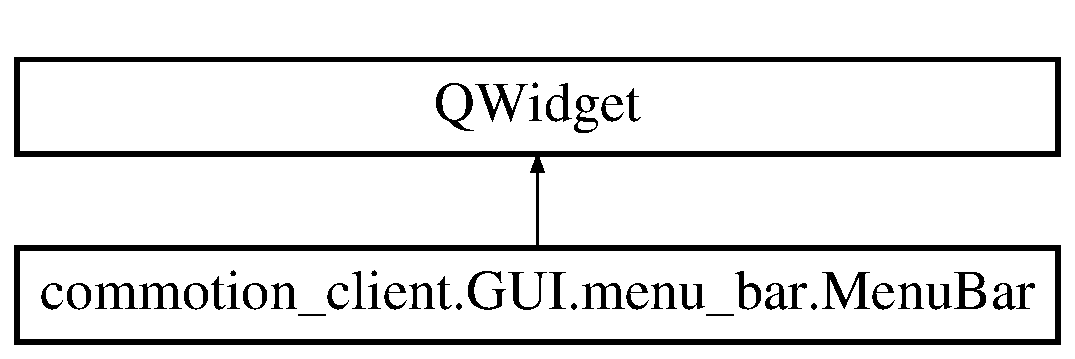
\includegraphics[height=2.000000cm]{classcommotion__client_1_1GUI_1_1menu__bar_1_1MenuBar}
\end{center}
\end{figure}
\subsection*{Public Member Functions}
\begin{DoxyCompactItemize}
\item 
\hypertarget{classcommotion__client_1_1GUI_1_1menu__bar_1_1MenuBar_a1f9817bd9c7f2dde1cc33aaec29151a9}{def {\bfseries \-\_\-\-\_\-init\-\_\-\-\_\-}}\label{classcommotion__client_1_1GUI_1_1menu__bar_1_1MenuBar_a1f9817bd9c7f2dde1cc33aaec29151a9}

\item 
def \hyperlink{classcommotion__client_1_1GUI_1_1menu__bar_1_1MenuBar_af0829b0f4a27a6246efbbe8c4412a283}{request\-\_\-viewport}
\item 
def \hyperlink{classcommotion__client_1_1GUI_1_1menu__bar_1_1MenuBar_aef9fda2956e1fffd9abbfbe420716519}{clear\-\_\-layout}
\item 
def \hyperlink{classcommotion__client_1_1GUI_1_1menu__bar_1_1MenuBar_a3ebeac5b69ad7004325183b547b3648a}{populate\-\_\-menu}
\item 
def \hyperlink{classcommotion__client_1_1GUI_1_1menu__bar_1_1MenuBar_a963ca3542a8f9ee6c8e8534fe530d443}{get\-\_\-parents}
\item 
def \hyperlink{classcommotion__client_1_1GUI_1_1menu__bar_1_1MenuBar_a7bbc3f3ab719dadb7943780dd17f1e82}{add\-\_\-menu\-\_\-item}
\end{DoxyCompactItemize}
\subsection*{Public Attributes}
\begin{DoxyCompactItemize}
\item 
\hypertarget{classcommotion__client_1_1GUI_1_1menu__bar_1_1MenuBar_a43b84a445a05f441662320e5f26b5599}{{\bfseries layout}}\label{classcommotion__client_1_1GUI_1_1menu__bar_1_1MenuBar_a43b84a445a05f441662320e5f26b5599}

\item 
\hypertarget{classcommotion__client_1_1GUI_1_1menu__bar_1_1MenuBar_a2397d4b257aa499bf1ef5da6e5b5faea}{{\bfseries log}}\label{classcommotion__client_1_1GUI_1_1menu__bar_1_1MenuBar_a2397d4b257aa499bf1ef5da6e5b5faea}

\item 
\hypertarget{classcommotion__client_1_1GUI_1_1menu__bar_1_1MenuBar_ad97dbe989a68d0453584c7c95137b8b4}{{\bfseries translate}}\label{classcommotion__client_1_1GUI_1_1menu__bar_1_1MenuBar_ad97dbe989a68d0453584c7c95137b8b4}

\item 
\hypertarget{classcommotion__client_1_1GUI_1_1menu__bar_1_1MenuBar_a967f47cfbc1348e41bc11026fb9ff0ac}{{\bfseries ext\-\_\-mgr}}\label{classcommotion__client_1_1GUI_1_1menu__bar_1_1MenuBar_a967f47cfbc1348e41bc11026fb9ff0ac}

\end{DoxyCompactItemize}
\subsection*{Static Public Attributes}
\begin{DoxyCompactItemize}
\item 
\hypertarget{classcommotion__client_1_1GUI_1_1menu__bar_1_1MenuBar_a10d4ce58617e1125c7f7e43512bc960a}{tuple {\bfseries viewport\-\_\-requested} = Qt\-Core.\-pyqt\-Signal(str)}\label{classcommotion__client_1_1GUI_1_1menu__bar_1_1MenuBar_a10d4ce58617e1125c7f7e43512bc960a}

\end{DoxyCompactItemize}


\subsection{Member Function Documentation}
\hypertarget{classcommotion__client_1_1GUI_1_1menu__bar_1_1MenuBar_a7bbc3f3ab719dadb7943780dd17f1e82}{\index{commotion\-\_\-client\-::\-G\-U\-I\-::menu\-\_\-bar\-::\-Menu\-Bar@{commotion\-\_\-client\-::\-G\-U\-I\-::menu\-\_\-bar\-::\-Menu\-Bar}!add\-\_\-menu\-\_\-item@{add\-\_\-menu\-\_\-item}}
\index{add\-\_\-menu\-\_\-item@{add\-\_\-menu\-\_\-item}!commotion_client::GUI::menu_bar::MenuBar@{commotion\-\_\-client\-::\-G\-U\-I\-::menu\-\_\-bar\-::\-Menu\-Bar}}
\subsubsection[{add\-\_\-menu\-\_\-item}]{\setlength{\rightskip}{0pt plus 5cm}def commotion\-\_\-client.\-G\-U\-I.\-menu\-\_\-bar.\-Menu\-Bar.\-add\-\_\-menu\-\_\-item (
\begin{DoxyParamCaption}
\item[{}]{self, }
\item[{}]{parent}
\end{DoxyParamCaption}
)}}\label{classcommotion__client_1_1GUI_1_1menu__bar_1_1MenuBar_a7bbc3f3ab719dadb7943780dd17f1e82}
\begin{DoxyVerb}Creates and returns a single top level menu item with cascading sub-menu items.

Args:
parent (string): The "parent" the top level menu item that is being requested.

Returns:
A tuple containing a top level button and its hidden sub-menu items.        
\end{DoxyVerb}
 

References commotion\-\_\-client.\-G\-U\-I.\-menu\-\_\-bar.\-Menu\-Bar.\-request\-\_\-viewport(), commotion\-\_\-client.\-G\-U\-I.\-menu\-\_\-bar.\-Menu\-Bar.\-translate, commotion\-\_\-client.\-extensions.\-config\-\_\-editor.\-main.\-View\-Port.\-translate, commotion\-\_\-client.\-G\-U\-I.\-main\-\_\-window.\-Main\-Window.\-translate, commotion\-\_\-client.\-G\-U\-I.\-extension\-\_\-toolbar.\-Extension\-Tool\-Bar.\-translate, commotion\-\_\-client.\-G\-U\-I.\-extension\-\_\-toolbar.\-Menu\-Item.\-translate, and commotion\-\_\-client.\-commotion\-\_\-client.\-Commotion\-Client\-Application.\-translate.



Referenced by commotion\-\_\-client.\-G\-U\-I.\-menu\-\_\-bar.\-Menu\-Bar.\-populate\-\_\-menu().


\begin{DoxyCode}
125 
126     \textcolor{keyword}{def }\hyperlink{classcommotion__client_1_1GUI_1_1menu__bar_1_1MenuBar_a7bbc3f3ab719dadb7943780dd17f1e82}{add\_menu\_item}(self, parent):
127         \textcolor{stringliteral}{"""Creates and returns a single top level menu item with cascading sub-menu items.}
128 \textcolor{stringliteral}{                }
129 \textcolor{stringliteral}{        Args:}
130 \textcolor{stringliteral}{        parent (string): The "parent" the top level menu item that is being requested.}
131 \textcolor{stringliteral}{        }
132 \textcolor{stringliteral}{        Returns:}
133 \textcolor{stringliteral}{        A tuple containing a top level button and its hidden sub-menu items.        }
134 \textcolor{stringliteral}{        """}
135         extensions = self.ext\_mgr.get\_extension\_from\_property(\textcolor{stringliteral}{'parent'}, parent)
136         \textcolor{keywordflow}{if} \textcolor{keywordflow}{not} extensions:
137             \textcolor{keywordflow}{raise} NameError(self.\hyperlink{classcommotion__client_1_1GUI_1_1menu__bar_1_1MenuBar_ad97dbe989a68d0453584c7c95137b8b4}{translate}(\textcolor{stringliteral}{"logs"}, \textcolor{stringliteral}{"No extensions found under the parent item \{0\}.
      "}.format(parent)))
138         \textcolor{comment}{#Create Top level item button}
139         title\_button = QtGui.QPushButton(QtCore.QCoreApplication.translate(\textcolor{stringliteral}{"Menu Item"}, parent))
140         title\_button.setCheckable(\textcolor{keyword}{True})
141         \textcolor{comment}{#Create sub-menu}
142         sub\_menu = QtGui.QFrame()
143         sub\_menu\_layout = QtGui.QVBoxLayout()
144         \textcolor{comment}{#populate the sub-menu item table.}
145         \textcolor{keywordflow}{for} ext \textcolor{keywordflow}{in} extensions:
146             sub\_menu\_item = \hyperlink{classcommotion__client_1_1GUI_1_1menu__bar_1_1subMenuWidget}{subMenuWidget}(self)
147             \textcolor{keywordflow}{try}:
148                 menu\_item\_title = self.ext\_mgr.get\_property(ext, \textcolor{stringliteral}{'menu\_item'})
149             \textcolor{keywordflow}{except} KeyError:
150                 menu\_item\_title = ext
151             sub\_menu\_item.setText(QtCore.QCoreApplication.translate(\textcolor{stringliteral}{"Sub-Menu Item"}, menu\_item\_title))
152             \textcolor{comment}{#We use partial here to pass a variable along when we attach the "clicked()" signal to the
       MenuBars requestViewport function}
153             sub\_menu\_item.clicked.connect(partial(self.\hyperlink{classcommotion__client_1_1GUI_1_1menu__bar_1_1MenuBar_af0829b0f4a27a6246efbbe8c4412a283}{request\_viewport}, ext))
154             sub\_menu\_layout.addWidget(sub\_menu\_item)
155         sub\_menu.setLayout(sub\_menu\_layout)
156         sub\_menu.hide()
157         \textcolor{comment}{#Connect toggle on out checkable title button to the visability of our subMenu}
158         title\_button.toggled.connect(sub\_menu.setVisible)
159         \textcolor{comment}{#package and return top level item and its corresponding subMenu}
160         section = (title\_button, sub\_menu)
161         \textcolor{keywordflow}{return} section
162 

\end{DoxyCode}
\hypertarget{classcommotion__client_1_1GUI_1_1menu__bar_1_1MenuBar_aef9fda2956e1fffd9abbfbe420716519}{\index{commotion\-\_\-client\-::\-G\-U\-I\-::menu\-\_\-bar\-::\-Menu\-Bar@{commotion\-\_\-client\-::\-G\-U\-I\-::menu\-\_\-bar\-::\-Menu\-Bar}!clear\-\_\-layout@{clear\-\_\-layout}}
\index{clear\-\_\-layout@{clear\-\_\-layout}!commotion_client::GUI::menu_bar::MenuBar@{commotion\-\_\-client\-::\-G\-U\-I\-::menu\-\_\-bar\-::\-Menu\-Bar}}
\subsubsection[{clear\-\_\-layout}]{\setlength{\rightskip}{0pt plus 5cm}def commotion\-\_\-client.\-G\-U\-I.\-menu\-\_\-bar.\-Menu\-Bar.\-clear\-\_\-layout (
\begin{DoxyParamCaption}
\item[{}]{self, }
\item[{}]{layout}
\end{DoxyParamCaption}
)}}\label{classcommotion__client_1_1GUI_1_1menu__bar_1_1MenuBar_aef9fda2956e1fffd9abbfbe420716519}
\begin{DoxyVerb}Clears a layout of all widgets.
 
Args:
layout (QLayout): A QLayout object that needs to be cleared of all objects.
\end{DoxyVerb}
 

References commotion\-\_\-client.\-G\-U\-I.\-menu\-\_\-bar.\-Menu\-Bar.\-clear\-\_\-layout().



Referenced by commotion\-\_\-client.\-G\-U\-I.\-menu\-\_\-bar.\-Menu\-Bar.\-clear\-\_\-layout(), and commotion\-\_\-client.\-G\-U\-I.\-menu\-\_\-bar.\-Menu\-Bar.\-populate\-\_\-menu().


\begin{DoxyCode}
54 
55     \textcolor{keyword}{def }\hyperlink{classcommotion__client_1_1GUI_1_1menu__bar_1_1MenuBar_aef9fda2956e1fffd9abbfbe420716519}{clear\_layout}(self, layout):
56         \textcolor{stringliteral}{"""Clears a layout of all widgets.}
57 \textcolor{stringliteral}{ }
58 \textcolor{stringliteral}{        Args:}
59 \textcolor{stringliteral}{        layout (QLayout): A QLayout object that needs to be cleared of all objects.}
60 \textcolor{stringliteral}{        """}        
61         \textcolor{keywordflow}{if} \textcolor{keywordflow}{not} layout.isEmpty():
62             \textcolor{keywordflow}{while} layout.count():
63                 item = layout.takeAt(0)
64                 widget = item.widget()
65                 \textcolor{keywordflow}{if} widget \textcolor{keywordflow}{is} \textcolor{keywordflow}{not} \textcolor{keywordtype}{None}:
66                     widget.deleteLater()
67                 \textcolor{keywordflow}{else}:
68                     self.\hyperlink{classcommotion__client_1_1GUI_1_1menu__bar_1_1MenuBar_aef9fda2956e1fffd9abbfbe420716519}{clear\_layout}(item.layout())

\end{DoxyCode}
\hypertarget{classcommotion__client_1_1GUI_1_1menu__bar_1_1MenuBar_a963ca3542a8f9ee6c8e8534fe530d443}{\index{commotion\-\_\-client\-::\-G\-U\-I\-::menu\-\_\-bar\-::\-Menu\-Bar@{commotion\-\_\-client\-::\-G\-U\-I\-::menu\-\_\-bar\-::\-Menu\-Bar}!get\-\_\-parents@{get\-\_\-parents}}
\index{get\-\_\-parents@{get\-\_\-parents}!commotion_client::GUI::menu_bar::MenuBar@{commotion\-\_\-client\-::\-G\-U\-I\-::menu\-\_\-bar\-::\-Menu\-Bar}}
\subsubsection[{get\-\_\-parents}]{\setlength{\rightskip}{0pt plus 5cm}def commotion\-\_\-client.\-G\-U\-I.\-menu\-\_\-bar.\-Menu\-Bar.\-get\-\_\-parents (
\begin{DoxyParamCaption}
\item[{}]{self, }
\item[{}]{extension\-\_\-list}
\end{DoxyParamCaption}
)}}\label{classcommotion__client_1_1GUI_1_1menu__bar_1_1MenuBar_a963ca3542a8f9ee6c8e8534fe530d443}
\begin{DoxyVerb}Gets all unique parents from a list of extensions.

This function gets the "parent" menu items from a list of extensions and returns a list of the unique members.

Args:
  extension_list (list): A list containing a set of strings that list the names of extensions.

Returns:
  A list of all the unique parents of the given extensions.

    ['parent item 01', 'parent item 02']
\end{DoxyVerb}
 

References commotion\-\_\-client.\-G\-U\-I.\-menu\-\_\-bar.\-Menu\-Bar.\-translate, commotion\-\_\-client.\-extensions.\-config\-\_\-editor.\-main.\-View\-Port.\-translate, commotion\-\_\-client.\-G\-U\-I.\-main\-\_\-window.\-Main\-Window.\-translate, commotion\-\_\-client.\-G\-U\-I.\-extension\-\_\-toolbar.\-Extension\-Tool\-Bar.\-translate, commotion\-\_\-client.\-G\-U\-I.\-extension\-\_\-toolbar.\-Menu\-Item.\-translate, and commotion\-\_\-client.\-commotion\-\_\-client.\-Commotion\-Client\-Application.\-translate.



Referenced by commotion\-\_\-client.\-G\-U\-I.\-menu\-\_\-bar.\-Menu\-Bar.\-populate\-\_\-menu().


\begin{DoxyCode}
100 
101     \textcolor{keyword}{def }\hyperlink{classcommotion__client_1_1GUI_1_1menu__bar_1_1MenuBar_a963ca3542a8f9ee6c8e8534fe530d443}{get\_parents}(self, extension\_list):
102         \textcolor{stringliteral}{"""Gets all unique parents from a list of extensions.}
103 \textcolor{stringliteral}{}
104 \textcolor{stringliteral}{        This function gets the "parent" menu items from a list of extensions and returns a list of the
       unique members.}
105 \textcolor{stringliteral}{}
106 \textcolor{stringliteral}{        Args:}
107 \textcolor{stringliteral}{          extension\_list (list): A list containing a set of strings that list the names of extensions.}
108 \textcolor{stringliteral}{}
109 \textcolor{stringliteral}{        Returns:}
110 \textcolor{stringliteral}{          A list of all the unique parents of the given extensions.}
111 \textcolor{stringliteral}{        }
112 \textcolor{stringliteral}{            ['parent item 01', 'parent item 02']}
113 \textcolor{stringliteral}{        """}
114         parents = []
115         \textcolor{keywordflow}{for} ext \textcolor{keywordflow}{in} extension\_list:
116             \textcolor{keywordflow}{try}:
117                 parent = self.ext\_mgr.get\_property(ext, \textcolor{stringliteral}{"parent"})
118             \textcolor{keywordflow}{except} KeyError:
119                 self.log.debug(self.\hyperlink{classcommotion__client_1_1GUI_1_1menu__bar_1_1MenuBar_ad97dbe989a68d0453584c7c95137b8b4}{translate}(\textcolor{stringliteral}{"logs"}, \textcolor{stringliteral}{"Config for \{0\} does not contain a \{1\}
       value. Setting \{1\} to default value."}.format(ext, \textcolor{stringliteral}{"parent"})))
120                 parent = \textcolor{stringliteral}{"Extensions"}
121             \textcolor{keywordflow}{if} parent \textcolor{keywordflow}{not} \textcolor{keywordflow}{in} parents:
122                 parents.append(parent)
123         \textcolor{keywordflow}{return} parents
124 

\end{DoxyCode}
\hypertarget{classcommotion__client_1_1GUI_1_1menu__bar_1_1MenuBar_a3ebeac5b69ad7004325183b547b3648a}{\index{commotion\-\_\-client\-::\-G\-U\-I\-::menu\-\_\-bar\-::\-Menu\-Bar@{commotion\-\_\-client\-::\-G\-U\-I\-::menu\-\_\-bar\-::\-Menu\-Bar}!populate\-\_\-menu@{populate\-\_\-menu}}
\index{populate\-\_\-menu@{populate\-\_\-menu}!commotion_client::GUI::menu_bar::MenuBar@{commotion\-\_\-client\-::\-G\-U\-I\-::menu\-\_\-bar\-::\-Menu\-Bar}}
\subsubsection[{populate\-\_\-menu}]{\setlength{\rightskip}{0pt plus 5cm}def commotion\-\_\-client.\-G\-U\-I.\-menu\-\_\-bar.\-Menu\-Bar.\-populate\-\_\-menu (
\begin{DoxyParamCaption}
\item[{}]{self}
\end{DoxyParamCaption}
)}}\label{classcommotion__client_1_1GUI_1_1menu__bar_1_1MenuBar_a3ebeac5b69ad7004325183b547b3648a}
\begin{DoxyVerb}Resets and populates the menu using loaded extensions.\end{DoxyVerb}
 

References commotion\-\_\-client.\-G\-U\-I.\-menu\-\_\-bar.\-Menu\-Bar.\-add\-\_\-menu\-\_\-item(), commotion\-\_\-client.\-G\-U\-I.\-menu\-\_\-bar.\-Menu\-Bar.\-clear\-\_\-layout(), commotion\-\_\-client.\-G\-U\-I.\-menu\-\_\-bar.\-Menu\-Bar.\-get\-\_\-parents(), commotion\-\_\-client.\-G\-U\-I.\-menu\-\_\-bar.\-Menu\-Bar.\-layout, commotion\-\_\-client.\-G\-U\-I.\-menu\-\_\-bar.\-Menu\-Bar.\-translate, commotion\-\_\-client.\-extensions.\-config\-\_\-editor.\-main.\-View\-Port.\-translate, commotion\-\_\-client.\-G\-U\-I.\-main\-\_\-window.\-Main\-Window.\-translate, commotion\-\_\-client.\-G\-U\-I.\-extension\-\_\-toolbar.\-Extension\-Tool\-Bar.\-translate, commotion\-\_\-client.\-G\-U\-I.\-extension\-\_\-toolbar.\-Menu\-Item.\-translate, and commotion\-\_\-client.\-commotion\-\_\-client.\-Commotion\-Client\-Application.\-translate.


\begin{DoxyCode}
69 
70     \textcolor{keyword}{def }\hyperlink{classcommotion__client_1_1GUI_1_1menu__bar_1_1MenuBar_a3ebeac5b69ad7004325183b547b3648a}{populate\_menu}(self):
71         \textcolor{stringliteral}{"""Resets and populates the menu using loaded extensions."""}
72         \textcolor{keywordflow}{if} \textcolor{keywordflow}{not} self.layout.isEmpty():
73             self.\hyperlink{classcommotion__client_1_1GUI_1_1menu__bar_1_1MenuBar_aef9fda2956e1fffd9abbfbe420716519}{clear\_layout}(self.\hyperlink{classcommotion__client_1_1GUI_1_1menu__bar_1_1MenuBar_a43b84a445a05f441662320e5f26b5599}{layout})
74         menu\_items = \{\}
75         \textcolor{keywordflow}{if} \textcolor{keywordflow}{not} self.ext\_mgr.check\_installed():
76             self.ext\_mgr.init\_extension\_libraries()
77         extensions = self.ext\_mgr.get\_installed().keys()
78         \textcolor{keywordflow}{if} extensions:
79             top\_level = self.\hyperlink{classcommotion__client_1_1GUI_1_1menu__bar_1_1MenuBar_a963ca3542a8f9ee6c8e8534fe530d443}{get\_parents}(extensions)
80             \textcolor{keywordflow}{for} top\_level\_item \textcolor{keywordflow}{in} top\_level:
81                 \textcolor{keywordflow}{try}:
82                     current\_item = self.\hyperlink{classcommotion__client_1_1GUI_1_1menu__bar_1_1MenuBar_a7bbc3f3ab719dadb7943780dd17f1e82}{add\_menu\_item}(top\_level\_item)
83                 \textcolor{keywordflow}{except} NameError \textcolor{keyword}{as} \_excpt:
84                     self.log.debug(self.\hyperlink{classcommotion__client_1_1GUI_1_1menu__bar_1_1MenuBar_ad97dbe989a68d0453584c7c95137b8b4}{translate}(\textcolor{stringliteral}{"logs"}, \textcolor{stringliteral}{"No extensions found under the parent
       item \{0\}. Parent item will not be added to the menu."}.format(top\_level\_item)))
85                     self.log.exception(\_excpt)
86                 \textcolor{keywordflow}{else}:
87                     \textcolor{keywordflow}{if} current\_item:
88                         menu\_items[top\_level\_item] = current\_item
89             \textcolor{keywordflow}{if} menu\_items:
90                 \textcolor{keywordflow}{for} title, section \textcolor{keywordflow}{in} menu\_items.items():
91                     \textcolor{comment}{#Add top level menu item}
92                     self.layout.addWidget(section[0])
93                     \textcolor{comment}{#Add sub-menu layout}
94                     self.layout.addWidget(section[1])
95             \textcolor{keywordflow}{else}:
96                 \textcolor{keywordflow}{raise} AttributeError(QtCore.QCoreApplication.translate(\textcolor{stringliteral}{"exception"}, \textcolor{stringliteral}{"No menu items could be
       created from the extensions found. Please re-run the commotion client with full verbosity to identify what
       went wrong."}))
97         \textcolor{keywordflow}{else}:
98             \textcolor{keywordflow}{raise} NameError(QtCore.QCoreApplication.translate(\textcolor{stringliteral}{"exception"}, \textcolor{stringliteral}{"No extensions found. Please
       re-run the commotion\_client with full verbosity to find out what went wrong."}))
99         self.setLayout(self.\hyperlink{classcommotion__client_1_1GUI_1_1menu__bar_1_1MenuBar_a43b84a445a05f441662320e5f26b5599}{layout})
        
\end{DoxyCode}
\hypertarget{classcommotion__client_1_1GUI_1_1menu__bar_1_1MenuBar_af0829b0f4a27a6246efbbe8c4412a283}{\index{commotion\-\_\-client\-::\-G\-U\-I\-::menu\-\_\-bar\-::\-Menu\-Bar@{commotion\-\_\-client\-::\-G\-U\-I\-::menu\-\_\-bar\-::\-Menu\-Bar}!request\-\_\-viewport@{request\-\_\-viewport}}
\index{request\-\_\-viewport@{request\-\_\-viewport}!commotion_client::GUI::menu_bar::MenuBar@{commotion\-\_\-client\-::\-G\-U\-I\-::menu\-\_\-bar\-::\-Menu\-Bar}}
\subsubsection[{request\-\_\-viewport}]{\setlength{\rightskip}{0pt plus 5cm}def commotion\-\_\-client.\-G\-U\-I.\-menu\-\_\-bar.\-Menu\-Bar.\-request\-\_\-viewport (
\begin{DoxyParamCaption}
\item[{}]{self, }
\item[{}]{viewport}
\end{DoxyParamCaption}
)}}\label{classcommotion__client_1_1GUI_1_1menu__bar_1_1MenuBar_af0829b0f4a27a6246efbbe8c4412a283}
\begin{DoxyVerb}When called will emit a request for a viewport change.
\end{DoxyVerb}
 

Referenced by commotion\-\_\-client.\-G\-U\-I.\-menu\-\_\-bar.\-Menu\-Bar.\-add\-\_\-menu\-\_\-item().


\begin{DoxyCode}
47 
48     \textcolor{keyword}{def }\hyperlink{classcommotion__client_1_1GUI_1_1menu__bar_1_1MenuBar_af0829b0f4a27a6246efbbe8c4412a283}{request\_viewport}(self, viewport):
49         \textcolor{stringliteral}{"""}
50 \textcolor{stringliteral}{        When called will emit a request for a viewport change.}
51 \textcolor{stringliteral}{        """}
52         self.log.debug(QtCore.QCoreApplication.translate(\textcolor{stringliteral}{"logs"}, \textcolor{stringliteral}{"Request to change viewport sent"}))
53         self.viewport\_requested.emit(viewport)
        
\end{DoxyCode}


The documentation for this class was generated from the following file\-:\begin{DoxyCompactItemize}
\item 
commotion\-\_\-client/\-G\-U\-I/menu\-\_\-bar.\-py\end{DoxyCompactItemize}

\hypertarget{classcommotion__client_1_1GUI_1_1extension__toolbar_1_1MenuItem}{\section{commotion\-\_\-client.\-G\-U\-I.\-extension\-\_\-toolbar.\-Menu\-Item Class Reference}
\label{classcommotion__client_1_1GUI_1_1extension__toolbar_1_1MenuItem}\index{commotion\-\_\-client.\-G\-U\-I.\-extension\-\_\-toolbar.\-Menu\-Item@{commotion\-\_\-client.\-G\-U\-I.\-extension\-\_\-toolbar.\-Menu\-Item}}
}
Inheritance diagram for commotion\-\_\-client.\-G\-U\-I.\-extension\-\_\-toolbar.\-Menu\-Item\-:\begin{figure}[H]
\begin{center}
\leavevmode
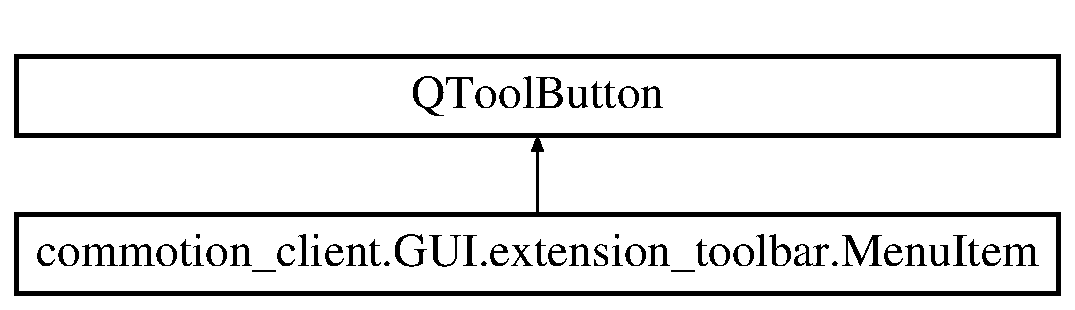
\includegraphics[height=2.000000cm]{classcommotion__client_1_1GUI_1_1extension__toolbar_1_1MenuItem}
\end{center}
\end{figure}
\subsection*{Public Member Functions}
\begin{DoxyCompactItemize}
\item 
def \hyperlink{classcommotion__client_1_1GUI_1_1extension__toolbar_1_1MenuItem_a111f98709fa79a9be8bdeed5722a9b69}{\-\_\-\-\_\-init\-\_\-\-\_\-}
\item 
\hypertarget{classcommotion__client_1_1GUI_1_1extension__toolbar_1_1MenuItem_a59af7fe77b05243a1ca6a4821565d8f2}{def {\bfseries set\-\_\-menu}}\label{classcommotion__client_1_1GUI_1_1extension__toolbar_1_1MenuItem_a59af7fe77b05243a1ca6a4821565d8f2}

\end{DoxyCompactItemize}
\subsection*{Public Attributes}
\begin{DoxyCompactItemize}
\item 
\hypertarget{classcommotion__client_1_1GUI_1_1extension__toolbar_1_1MenuItem_a6984ce2f476f256d285f1517d9beead6}{{\bfseries log}}\label{classcommotion__client_1_1GUI_1_1extension__toolbar_1_1MenuItem_a6984ce2f476f256d285f1517d9beead6}

\item 
\hypertarget{classcommotion__client_1_1GUI_1_1extension__toolbar_1_1MenuItem_a0134e71e4901cc4eec9b50785cba7265}{{\bfseries translate}}\label{classcommotion__client_1_1GUI_1_1extension__toolbar_1_1MenuItem_a0134e71e4901cc4eec9b50785cba7265}

\item 
\hypertarget{classcommotion__client_1_1GUI_1_1extension__toolbar_1_1MenuItem_a49032d0bb2b22e07d66a228d756d9350}{{\bfseries viewport}}\label{classcommotion__client_1_1GUI_1_1extension__toolbar_1_1MenuItem_a49032d0bb2b22e07d66a228d756d9350}

\item 
\hypertarget{classcommotion__client_1_1GUI_1_1extension__toolbar_1_1MenuItem_a6bc93d5526252a71a9543f75df2aeac6}{{\bfseries sub\-\_\-menu}}\label{classcommotion__client_1_1GUI_1_1extension__toolbar_1_1MenuItem_a6bc93d5526252a71a9543f75df2aeac6}

\end{DoxyCompactItemize}


\subsection{Detailed Description}
\begin{DoxyVerb}The menu_item template object

To Make a basic toolbar button simply run the following.

#From within the ExtensionToolBar
my_button = MenuItem
my_button.setIcon(self.icon.save)
my_button.setText(self.translate("menu", "Save"))
my_button.triggered.connect(self.my_save_function)

To Make a toolbar with a menu run the following.

#From within the ExtensionToolBar
my_menu = MenuItem
my_menu.setIcon(self.icon.settings)
my_menu.setText(self.translate("menu", "Options"))
my_menu.set_menu(True)
menu_save = QtGui.QAction("Save", icons.save, self.my_save_function)
my_menu.sub_menu.addAction(menu_save)
#Using a custom icon from an extension.
menu_load = QtGui.QAction("Load", QtGui.QIcon("icons/load.png"), statusTip=self.translate("menu", "Load a item from a file"), triggered=self.my_load_function)
my_menu.menu.addAction(menu_load)

menuItems are QToolButtons
menuItems that have sub menu's are composed of a QMenu with QActions within it.

QToolButton:http://pyqt.sourceforge.net/Docs/PyQt4/qtoolbutton.html
QMenu: http://pyqt.sourceforge.net/Docs/PyQt4/qmenu.html
QAction: http://pyqt.sourceforge.net/Docs/PyQt4/qaction.html\end{DoxyVerb}
 

\subsection{Constructor \& Destructor Documentation}
\hypertarget{classcommotion__client_1_1GUI_1_1extension__toolbar_1_1MenuItem_a111f98709fa79a9be8bdeed5722a9b69}{\index{commotion\-\_\-client\-::\-G\-U\-I\-::extension\-\_\-toolbar\-::\-Menu\-Item@{commotion\-\_\-client\-::\-G\-U\-I\-::extension\-\_\-toolbar\-::\-Menu\-Item}!\-\_\-\-\_\-init\-\_\-\-\_\-@{\-\_\-\-\_\-init\-\_\-\-\_\-}}
\index{\-\_\-\-\_\-init\-\_\-\-\_\-@{\-\_\-\-\_\-init\-\_\-\-\_\-}!commotion_client::GUI::extension_toolbar::MenuItem@{commotion\-\_\-client\-::\-G\-U\-I\-::extension\-\_\-toolbar\-::\-Menu\-Item}}
\subsubsection[{\-\_\-\-\_\-init\-\_\-\-\_\-}]{\setlength{\rightskip}{0pt plus 5cm}def commotion\-\_\-client.\-G\-U\-I.\-extension\-\_\-toolbar.\-Menu\-Item.\-\_\-\-\_\-init\-\_\-\-\_\- (
\begin{DoxyParamCaption}
\item[{}]{self, }
\item[{}]{parent = {\ttfamily None}, }
\item[{}]{viewport = {\ttfamily None}}
\end{DoxyParamCaption}
)}}\label{classcommotion__client_1_1GUI_1_1extension__toolbar_1_1MenuItem_a111f98709fa79a9be8bdeed5722a9b69}
\begin{DoxyVerb}Sets up all the core components needed for a minimal menuItem

Args:
  viewport (object): The current viewport. This allows menu_items to have its actions interact with the current viewport.\end{DoxyVerb}
 

References commotion\-\_\-client.\-G\-U\-I.\-extension\-\_\-toolbar.\-Extension\-Tool\-Bar.\-\_\-dirty, commotion\-\_\-client.\-extensions.\-config\-\_\-editor.\-main.\-View\-Port.\-\_\-dirty, commotion\-\_\-client.\-G\-U\-I.\-extension\-\_\-toolbar.\-Menu\-Item.\-\_\-dirty, commotion\-\_\-client.\-G\-U\-I.\-crash\-\_\-report.\-Crash\-Report.\-log, commotion\-\_\-client.\-extensions.\-config\-\_\-editor.\-main.\-View\-Port.\-log, commotion\-\_\-client.\-G\-U\-I.\-extension\-\_\-toolbar.\-Extension\-Tool\-Bar.\-log, commotion\-\_\-client.\-commotion\-\_\-client.\-Hold\-State\-During\-Restart.\-log, commotion\-\_\-client.\-G\-U\-I.\-extension\-\_\-toolbar.\-Menu\-Item.\-log, commotion\-\_\-client.\-G\-U\-I.\-crash\-\_\-report.\-Report\-Gatherer.\-log, commotion\-\_\-client.\-commotion\-\_\-client.\-Commotion\-Client\-Application.\-log, commotion\-\_\-client.\-G\-U\-I.\-extension\-\_\-toolbar.\-Menu\-Item.\-sub\-\_\-menu, commotion\-\_\-client.\-extensions.\-config\-\_\-editor.\-main.\-View\-Port.\-translate, commotion\-\_\-client.\-G\-U\-I.\-extension\-\_\-toolbar.\-Extension\-Tool\-Bar.\-translate, commotion\-\_\-client.\-G\-U\-I.\-extension\-\_\-toolbar.\-Menu\-Item.\-translate, commotion\-\_\-client.\-commotion\-\_\-client.\-Commotion\-Client\-Application.\-translate, commotion\-\_\-client.\-G\-U\-I.\-extension\-\_\-toolbar.\-Extension\-Tool\-Bar.\-viewport, and commotion\-\_\-client.\-G\-U\-I.\-extension\-\_\-toolbar.\-Menu\-Item.\-viewport.


\begin{DoxyCode}
97 
98     \textcolor{keyword}{def }\hyperlink{classcommotion__client_1_1GUI_1_1extension__toolbar_1_1MenuItem_a111f98709fa79a9be8bdeed5722a9b69}{\_\_init\_\_}(self, parent=None, viewport=None):
99         \textcolor{stringliteral}{"""Sets up all the core components needed for a minimal menuItem}
100 \textcolor{stringliteral}{        }
101 \textcolor{stringliteral}{        Args:}
102 \textcolor{stringliteral}{          viewport (object): The current viewport. This allows menu\_items to have its actions interact with
       the current viewport.}
103 \textcolor{stringliteral}{        }
104 \textcolor{stringliteral}{        """}
105         super().\hyperlink{classcommotion__client_1_1GUI_1_1extension__toolbar_1_1MenuItem_a111f98709fa79a9be8bdeed5722a9b69}{\_\_init\_\_}()
106         self.\hyperlink{classcommotion__client_1_1GUI_1_1extension__toolbar_1_1MenuItem_a3e3264241df55c41099f5f0f638d40f6}{\_dirty} = \textcolor{keyword}{False}
107         self.\hyperlink{classcommotion__client_1_1GUI_1_1extension__toolbar_1_1MenuItem_a6984ce2f476f256d285f1517d9beead6}{log} = logging.getLogger(\textcolor{stringliteral}{"commotion\_client."}+\_\_name\_\_)
108         self.\hyperlink{classcommotion__client_1_1GUI_1_1extension__toolbar_1_1MenuItem_a0134e71e4901cc4eec9b50785cba7265}{translate} = QtCore.QCoreApplication.translate
109         self.\hyperlink{classcommotion__client_1_1GUI_1_1extension__toolbar_1_1MenuItem_a49032d0bb2b22e07d66a228d756d9350}{viewport} = viewport
        
\end{DoxyCode}


The documentation for this class was generated from the following file\-:\begin{DoxyCompactItemize}
\item 
commotion\-\_\-client/\-G\-U\-I/extension\-\_\-toolbar.\-py\end{DoxyCompactItemize}

\hypertarget{classcommotion__client_1_1utils_1_1validate_1_1Networking}{\section{commotion\-\_\-client.\-utils.\-validate.\-Networking Class Reference}
\label{classcommotion__client_1_1utils_1_1validate_1_1Networking}\index{commotion\-\_\-client.\-utils.\-validate.\-Networking@{commotion\-\_\-client.\-utils.\-validate.\-Networking}}
}
Inheritance diagram for commotion\-\_\-client.\-utils.\-validate.\-Networking\-:\begin{figure}[H]
\begin{center}
\leavevmode
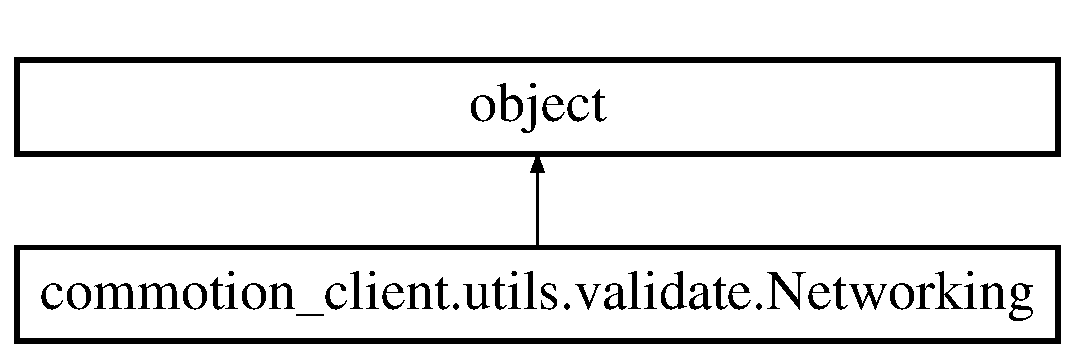
\includegraphics[height=2.000000cm]{classcommotion__client_1_1utils_1_1validate_1_1Networking}
\end{center}
\end{figure}
\subsection*{Public Member Functions}
\begin{DoxyCompactItemize}
\item 
\hypertarget{classcommotion__client_1_1utils_1_1validate_1_1Networking_af83f8af7dc9fd426c27d7fd214051edc}{def {\bfseries \-\_\-\-\_\-init\-\_\-\-\_\-}}\label{classcommotion__client_1_1utils_1_1validate_1_1Networking_af83f8af7dc9fd426c27d7fd214051edc}

\item 
def \hyperlink{classcommotion__client_1_1utils_1_1validate_1_1Networking_aaeee5dedbe589a997ddf820b17359c35}{ipaddr}
\end{DoxyCompactItemize}
\subsection*{Public Attributes}
\begin{DoxyCompactItemize}
\item 
\hypertarget{classcommotion__client_1_1utils_1_1validate_1_1Networking_af284adbbe8265ea379d64d3d6ee66342}{{\bfseries log}}\label{classcommotion__client_1_1utils_1_1validate_1_1Networking_af284adbbe8265ea379d64d3d6ee66342}

\item 
\hypertarget{classcommotion__client_1_1utils_1_1validate_1_1Networking_a2728d53728c499c4da34412a8b773216}{{\bfseries translate}}\label{classcommotion__client_1_1utils_1_1validate_1_1Networking_a2728d53728c499c4da34412a8b773216}

\end{DoxyCompactItemize}


\subsection{Member Function Documentation}
\hypertarget{classcommotion__client_1_1utils_1_1validate_1_1Networking_aaeee5dedbe589a997ddf820b17359c35}{\index{commotion\-\_\-client\-::utils\-::validate\-::\-Networking@{commotion\-\_\-client\-::utils\-::validate\-::\-Networking}!ipaddr@{ipaddr}}
\index{ipaddr@{ipaddr}!commotion_client::utils::validate::Networking@{commotion\-\_\-client\-::utils\-::validate\-::\-Networking}}
\subsubsection[{ipaddr}]{\setlength{\rightskip}{0pt plus 5cm}def commotion\-\_\-client.\-utils.\-validate.\-Networking.\-ipaddr (
\begin{DoxyParamCaption}
\item[{}]{self, }
\item[{}]{ip\-\_\-addr, }
\item[{}]{addr\-\_\-type = {\ttfamily None}}
\end{DoxyParamCaption}
)}}\label{classcommotion__client_1_1utils_1_1validate_1_1Networking_aaeee5dedbe589a997ddf820b17359c35}
\begin{DoxyVerb}Checks if a string is a validly formatted IPv4 or IPv6 address.

@param ip str A ip address to be checked
@param addr_type int The appropriate version number: 4 for IPv4, 6 for IPv6.
\end{DoxyVerb}
 

References commotion\-\_\-client.\-G\-U\-I.\-menu\-\_\-bar.\-Menu\-Bar.\-translate, commotion\-\_\-client.\-extensions.\-config\-\_\-editor.\-main.\-View\-Port.\-translate, commotion\-\_\-client.\-G\-U\-I.\-main\-\_\-window.\-Main\-Window.\-translate, commotion\-\_\-client.\-G\-U\-I.\-toolbar\-\_\-builder.\-Tool\-Bar.\-translate, commotion\-\_\-client.\-utils.\-validate.\-Client\-Config.\-translate, commotion\-\_\-client.\-G\-U\-I.\-extension\-\_\-toolbar.\-Extension\-Tool\-Bar.\-translate, commotion\-\_\-client.\-G\-U\-I.\-toolbar.\-Tool\-Bar.\-translate, commotion\-\_\-client.\-utils.\-extension\-\_\-manager.\-Extension\-Manager.\-translate, commotion\-\_\-client.\-G\-U\-I.\-extension\-\_\-toolbar.\-Menu\-Item.\-translate, commotion\-\_\-client.\-commotion\-\_\-client.\-Commotion\-Client\-Application.\-translate, commotion\-\_\-client.\-utils.\-validate.\-Networking.\-translate, and commotion\-\_\-client.\-utils.\-extension\-\_\-manager.\-Config\-Manager.\-translate.


\begin{DoxyCode}
323 
324     \textcolor{keyword}{def }\hyperlink{classcommotion__client_1_1utils_1_1validate_1_1Networking_aaeee5dedbe589a997ddf820b17359c35}{ipaddr}(self, ip\_addr, addr\_type=None):
325         \textcolor{stringliteral}{"""}
326 \textcolor{stringliteral}{        Checks if a string is a validly formatted IPv4 or IPv6 address.}
327 \textcolor{stringliteral}{}
328 \textcolor{stringliteral}{        @param ip str A ip address to be checked}
329 \textcolor{stringliteral}{        @param addr\_type int The appropriate version number: 4 for IPv4, 6 for IPv6.}
330 \textcolor{stringliteral}{        """}
331         \textcolor{keywordflow}{try}:
332             addr = ipaddress.ip\_address(str(ip\_addr))
333         \textcolor{keywordflow}{except} ValueError:
334             self.log.warning(self.\hyperlink{classcommotion__client_1_1utils_1_1validate_1_1Networking_a2728d53728c499c4da34412a8b773216}{translate}(\textcolor{stringliteral}{"logs"}, \textcolor{stringliteral}{"The value \{0\} is not an validly formed
       IP-address."}).format(ip\_addr))
335             \textcolor{keywordflow}{return} \textcolor{keyword}{False}
336         \textcolor{keywordflow}{if} addr\_type:
337             \textcolor{keywordflow}{if} addr.version == addr\_type:
338                 \textcolor{keywordflow}{return} \textcolor{keyword}{True}
339             \textcolor{keywordflow}{else}:
340                 self.log.warning(self.\hyperlink{classcommotion__client_1_1utils_1_1validate_1_1Networking_a2728d53728c499c4da34412a8b773216}{translate}(\textcolor{stringliteral}{"logs"}, \textcolor{stringliteral}{"The value \{0\} is not an validly formed
       IPv\{1\}-address."}).format(ip\_addr, addr\_type))
341                 \textcolor{keywordflow}{return} \textcolor{keyword}{False}
342         \textcolor{keywordflow}{else}:
343             \textcolor{keywordflow}{return} \textcolor{keyword}{True}
\end{DoxyCode}


The documentation for this class was generated from the following file\-:\begin{DoxyCompactItemize}
\item 
commotion\-\_\-client/utils/validate.\-py\end{DoxyCompactItemize}

\hypertarget{classcommotion__client_1_1GUI_1_1crash__report_1_1ReportGatherer}{\section{commotion\-\_\-client.\-G\-U\-I.\-crash\-\_\-report.\-Report\-Gatherer Class Reference}
\label{classcommotion__client_1_1GUI_1_1crash__report_1_1ReportGatherer}\index{commotion\-\_\-client.\-G\-U\-I.\-crash\-\_\-report.\-Report\-Gatherer@{commotion\-\_\-client.\-G\-U\-I.\-crash\-\_\-report.\-Report\-Gatherer}}
}
\subsection*{Public Member Functions}
\begin{DoxyCompactItemize}
\item 
\hypertarget{classcommotion__client_1_1GUI_1_1crash__report_1_1ReportGatherer_a8f8a67b02e968b01536846640e15a329}{def {\bfseries \-\_\-\-\_\-init\-\_\-\-\_\-}}\label{classcommotion__client_1_1GUI_1_1crash__report_1_1ReportGatherer_a8f8a67b02e968b01536846640e15a329}

\item 
\hypertarget{classcommotion__client_1_1GUI_1_1crash__report_1_1ReportGatherer_a8832cfd560db654afe5305d15c525021}{def {\bfseries get\-\_\-report}}\label{classcommotion__client_1_1GUI_1_1crash__report_1_1ReportGatherer_a8832cfd560db654afe5305d15c525021}

\item 
\hypertarget{classcommotion__client_1_1GUI_1_1crash__report_1_1ReportGatherer_aaaccb80d5b2e14dc5c3eadd900fc1635}{def {\bfseries add\-\_\-item}}\label{classcommotion__client_1_1GUI_1_1crash__report_1_1ReportGatherer_aaaccb80d5b2e14dc5c3eadd900fc1635}

\item 
\hypertarget{classcommotion__client_1_1GUI_1_1crash__report_1_1ReportGatherer_a14752ca72ce630765b24c08cfd0ac685}{def {\bfseries get\-\_\-defaults}}\label{classcommotion__client_1_1GUI_1_1crash__report_1_1ReportGatherer_a14752ca72ce630765b24c08cfd0ac685}

\end{DoxyCompactItemize}
\subsection*{Public Attributes}
\begin{DoxyCompactItemize}
\item 
\hypertarget{classcommotion__client_1_1GUI_1_1crash__report_1_1ReportGatherer_ada108101968c0e64bc0280724ab26746}{{\bfseries report}}\label{classcommotion__client_1_1GUI_1_1crash__report_1_1ReportGatherer_ada108101968c0e64bc0280724ab26746}

\item 
\hypertarget{classcommotion__client_1_1GUI_1_1crash__report_1_1ReportGatherer_a67341c89d29bb1bebd477cdfac2e22f7}{{\bfseries log}}\label{classcommotion__client_1_1GUI_1_1crash__report_1_1ReportGatherer_a67341c89d29bb1bebd477cdfac2e22f7}

\end{DoxyCompactItemize}


The documentation for this class was generated from the following file\-:\begin{DoxyCompactItemize}
\item 
commotion\-\_\-client/\-G\-U\-I/crash\-\_\-report.\-py\end{DoxyCompactItemize}

\hypertarget{classsettings_1_1Settings}{\section{settings.\+Settings Class Reference}
\label{classsettings_1_1Settings}\index{settings.\+Settings@{settings.\+Settings}}
}
Inheritance diagram for settings.\+Settings\+:\begin{figure}[H]
\begin{center}
\leavevmode
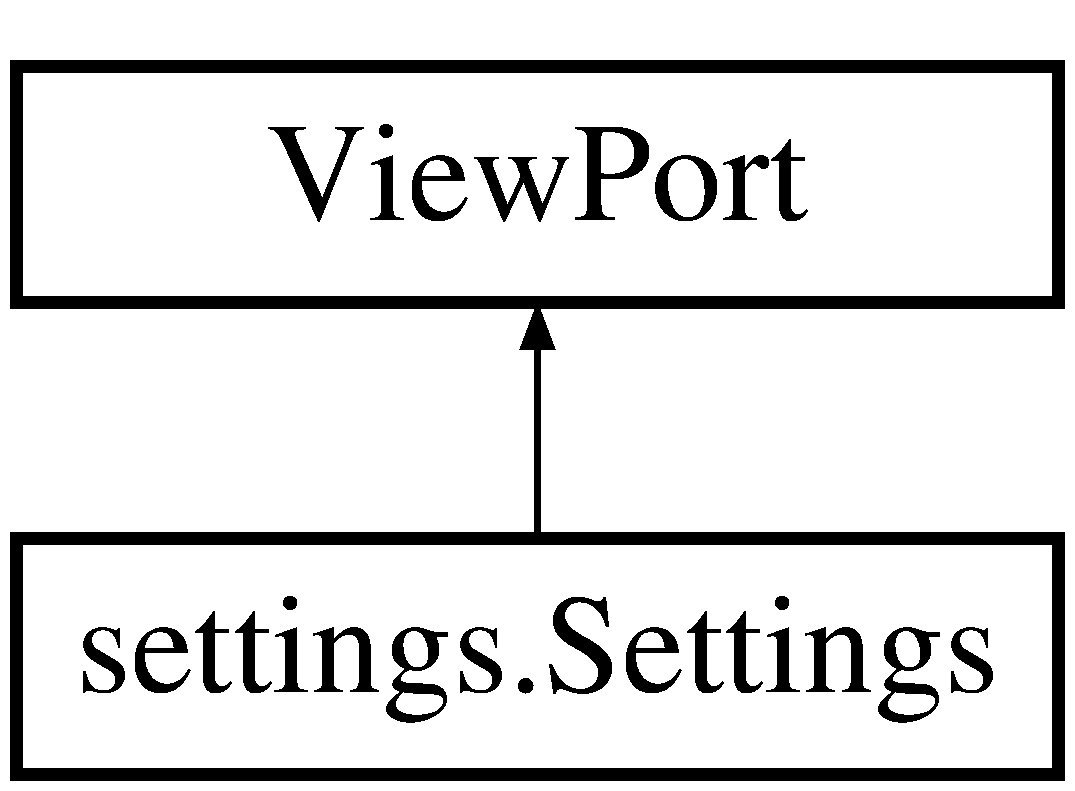
\includegraphics[height=2.000000cm]{classsettings_1_1Settings}
\end{center}
\end{figure}


\subsection{Detailed Description}
\begin{DoxyVerb}\end{DoxyVerb}
 

The documentation for this class was generated from the following file\+:\begin{DoxyCompactItemize}
\item 
docs/extensions/extension\+\_\+template/settings.\+py\end{DoxyCompactItemize}

\hypertarget{classcommotion__client_1_1extensions_1_1unit__test__mock_1_1main_1_1SettingsMenu}{\section{commotion\-\_\-client.\-extensions.\-unit\-\_\-test\-\_\-mock.\-main.\-Settings\-Menu Class Reference}
\label{classcommotion__client_1_1extensions_1_1unit__test__mock_1_1main_1_1SettingsMenu}\index{commotion\-\_\-client.\-extensions.\-unit\-\_\-test\-\_\-mock.\-main.\-Settings\-Menu@{commotion\-\_\-client.\-extensions.\-unit\-\_\-test\-\_\-mock.\-main.\-Settings\-Menu}}
}
Inheritance diagram for commotion\-\_\-client.\-extensions.\-unit\-\_\-test\-\_\-mock.\-main.\-Settings\-Menu\-:\begin{figure}[H]
\begin{center}
\leavevmode
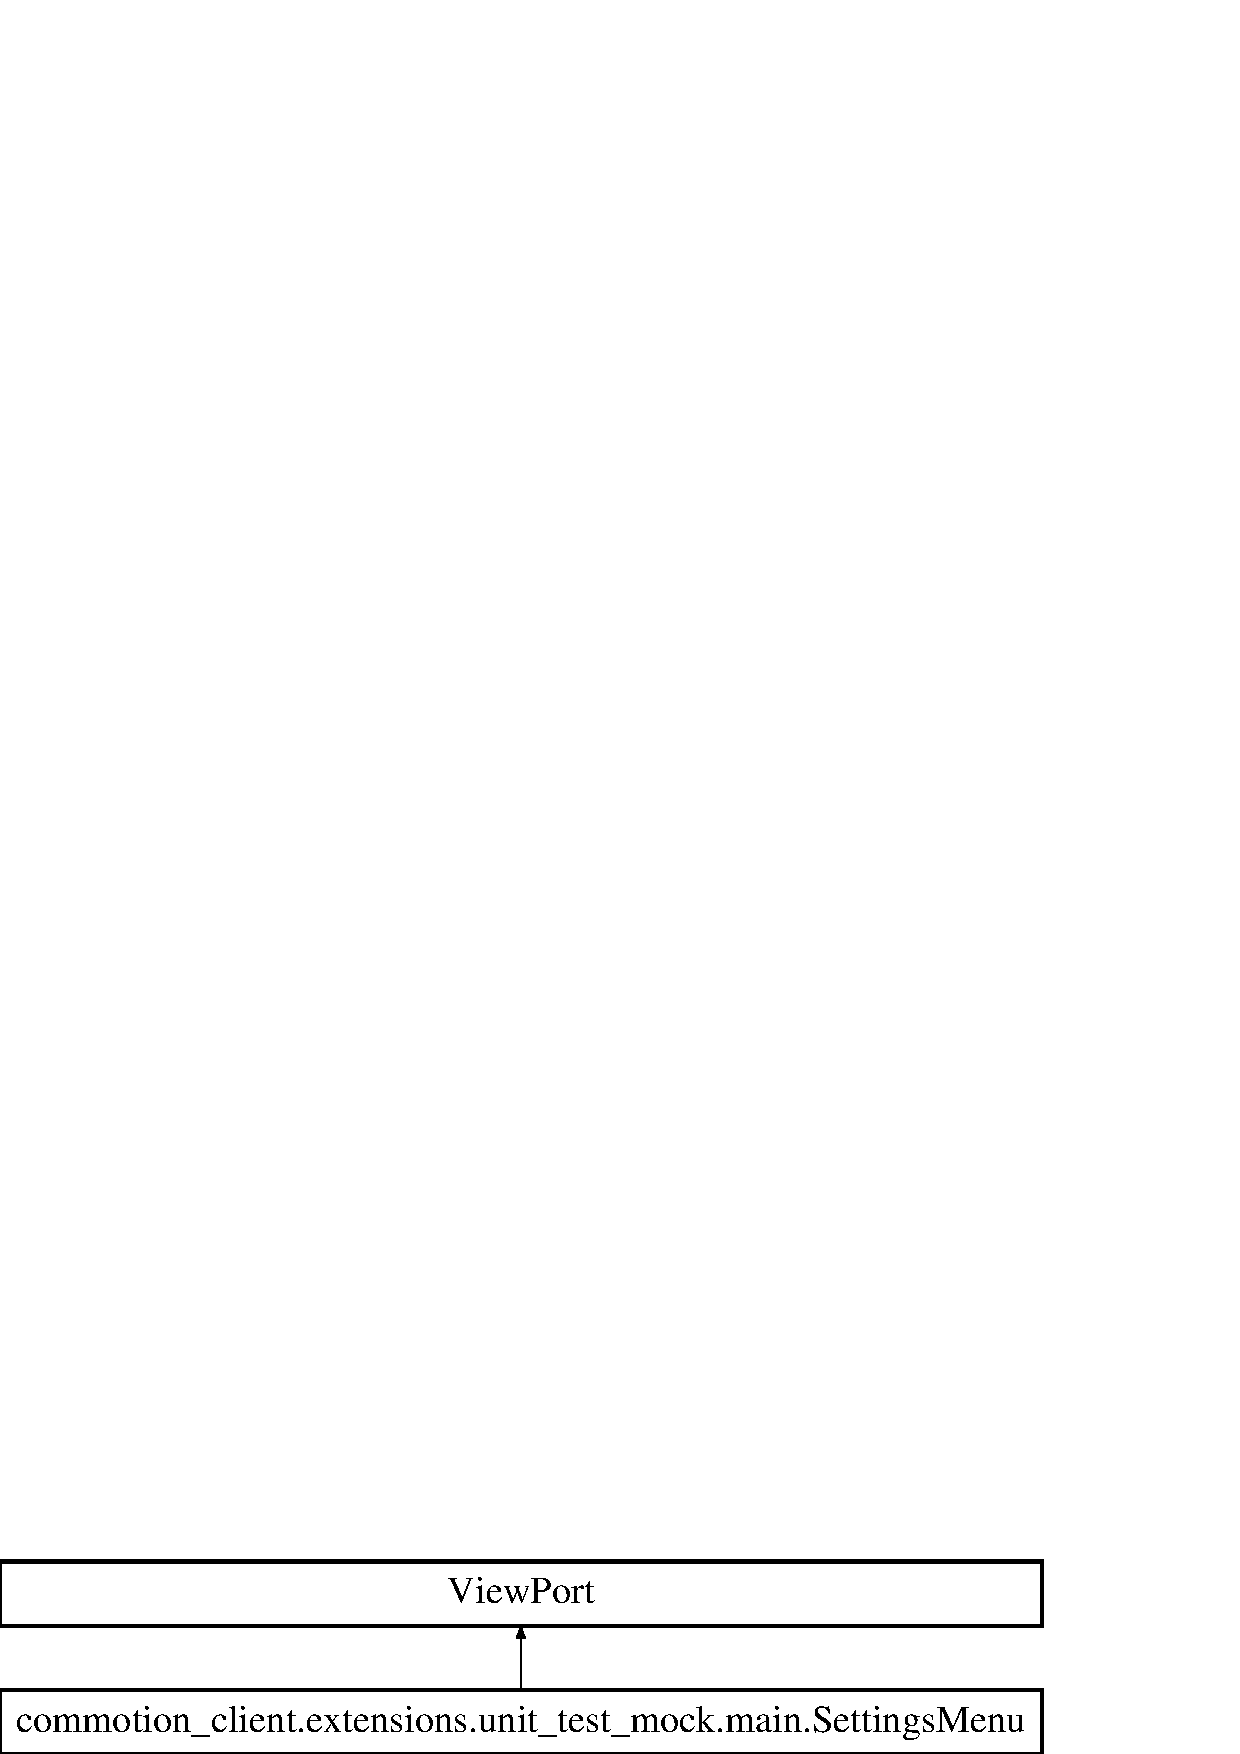
\includegraphics[height=2.000000cm]{classcommotion__client_1_1extensions_1_1unit__test__mock_1_1main_1_1SettingsMenu}
\end{center}
\end{figure}
\subsection*{Public Member Functions}
\begin{DoxyCompactItemize}
\item 
\hypertarget{classcommotion__client_1_1extensions_1_1unit__test__mock_1_1main_1_1SettingsMenu_adc3fb62d4e0b2011216723f07bd2694d}{def {\bfseries \-\_\-\-\_\-init\-\_\-\-\_\-}}\label{classcommotion__client_1_1extensions_1_1unit__test__mock_1_1main_1_1SettingsMenu_adc3fb62d4e0b2011216723f07bd2694d}

\item 
\hypertarget{classcommotion__client_1_1extensions_1_1unit__test__mock_1_1main_1_1SettingsMenu_a5e9a06e14061c35b87ffcc147f87ebb9}{def {\bfseries send\-\_\-signal}}\label{classcommotion__client_1_1extensions_1_1unit__test__mock_1_1main_1_1SettingsMenu_a5e9a06e14061c35b87ffcc147f87ebb9}

\item 
def \hyperlink{classcommotion__client_1_1extensions_1_1unit__test__mock_1_1main_1_1SettingsMenu_a12d8517f6e318038b3a57cf2f33907c4}{send\-\_\-error}
\item 
\hypertarget{classcommotion__client_1_1extensions_1_1unit__test__mock_1_1main_1_1SettingsMenu_ac74ab98887439dcafa298ab4610cb8c8}{def {\bfseries is\-\_\-loaded}}\label{classcommotion__client_1_1extensions_1_1unit__test__mock_1_1main_1_1SettingsMenu_ac74ab98887439dcafa298ab4610cb8c8}

\end{DoxyCompactItemize}
\subsection*{Static Public Attributes}
\begin{DoxyCompactItemize}
\item 
\hypertarget{classcommotion__client_1_1extensions_1_1unit__test__mock_1_1main_1_1SettingsMenu_a5f58582573674bfe07baf26ded7c3d36}{tuple {\bfseries start\-\_\-report\-\_\-collection} = Qt\-Core.\-pyqt\-Signal()}\label{classcommotion__client_1_1extensions_1_1unit__test__mock_1_1main_1_1SettingsMenu_a5f58582573674bfe07baf26ded7c3d36}

\item 
\hypertarget{classcommotion__client_1_1extensions_1_1unit__test__mock_1_1main_1_1SettingsMenu_abd351c2c4098be26a9eab3c6d7527aba}{tuple {\bfseries data\-\_\-report} = Qt\-Core.\-pyqt\-Signal(str, dict)}\label{classcommotion__client_1_1extensions_1_1unit__test__mock_1_1main_1_1SettingsMenu_abd351c2c4098be26a9eab3c6d7527aba}

\item 
\hypertarget{classcommotion__client_1_1extensions_1_1unit__test__mock_1_1main_1_1SettingsMenu_aaae06d25d6b08a0d8ececc278264a155}{tuple {\bfseries error\-\_\-report} = Qt\-Core.\-pyqt\-Signal(str)}\label{classcommotion__client_1_1extensions_1_1unit__test__mock_1_1main_1_1SettingsMenu_aaae06d25d6b08a0d8ececc278264a155}

\end{DoxyCompactItemize}


\subsection{Detailed Description}
\begin{DoxyVerb}This is a mock extension and should not be used for ANYTHING user facing!
\end{DoxyVerb}
 

\subsection{Member Function Documentation}
\hypertarget{classcommotion__client_1_1extensions_1_1unit__test__mock_1_1main_1_1SettingsMenu_a12d8517f6e318038b3a57cf2f33907c4}{\index{commotion\-\_\-client\-::extensions\-::unit\-\_\-test\-\_\-mock\-::main\-::\-Settings\-Menu@{commotion\-\_\-client\-::extensions\-::unit\-\_\-test\-\_\-mock\-::main\-::\-Settings\-Menu}!send\-\_\-error@{send\-\_\-error}}
\index{send\-\_\-error@{send\-\_\-error}!commotion_client::extensions::unit_test_mock::main::SettingsMenu@{commotion\-\_\-client\-::extensions\-::unit\-\_\-test\-\_\-mock\-::main\-::\-Settings\-Menu}}
\subsubsection[{send\-\_\-error}]{\setlength{\rightskip}{0pt plus 5cm}def commotion\-\_\-client.\-extensions.\-unit\-\_\-test\-\_\-mock.\-main.\-Settings\-Menu.\-send\-\_\-error (
\begin{DoxyParamCaption}
\item[{}]{self}
\end{DoxyParamCaption}
)}}\label{classcommotion__client_1_1extensions_1_1unit__test__mock_1_1main_1_1SettingsMenu_a12d8517f6e318038b3a57cf2f33907c4}
\begin{DoxyVerb}HI\end{DoxyVerb}
 
\begin{DoxyCode}
64 
65     \textcolor{keyword}{def }\hyperlink{classcommotion__client_1_1extensions_1_1unit__test__mock_1_1main_1_1SettingsMenu_a12d8517f6e318038b3a57cf2f33907c4}{send\_error}(self):
66         \textcolor{stringliteral}{"""HI"""}
67         self.error\_report.emit(\textcolor{stringliteral}{"THIS IS AN ERROR MESSAGE!!!"})
68         \textcolor{keywordflow}{pass}

\end{DoxyCode}


The documentation for this class was generated from the following file\-:\begin{DoxyCompactItemize}
\item 
commotion\-\_\-client/extensions/unit\-\_\-test\-\_\-mock/main.\-py\end{DoxyCompactItemize}

\hypertarget{classtest__suite_1_1SettingsTest}{\section{test\+\_\+suite.\+Settings\+Test Class Reference}
\label{classtest__suite_1_1SettingsTest}\index{test\+\_\+suite.\+Settings\+Test@{test\+\_\+suite.\+Settings\+Test}}
}
Inheritance diagram for test\+\_\+suite.\+Settings\+Test\+:\begin{figure}[H]
\begin{center}
\leavevmode
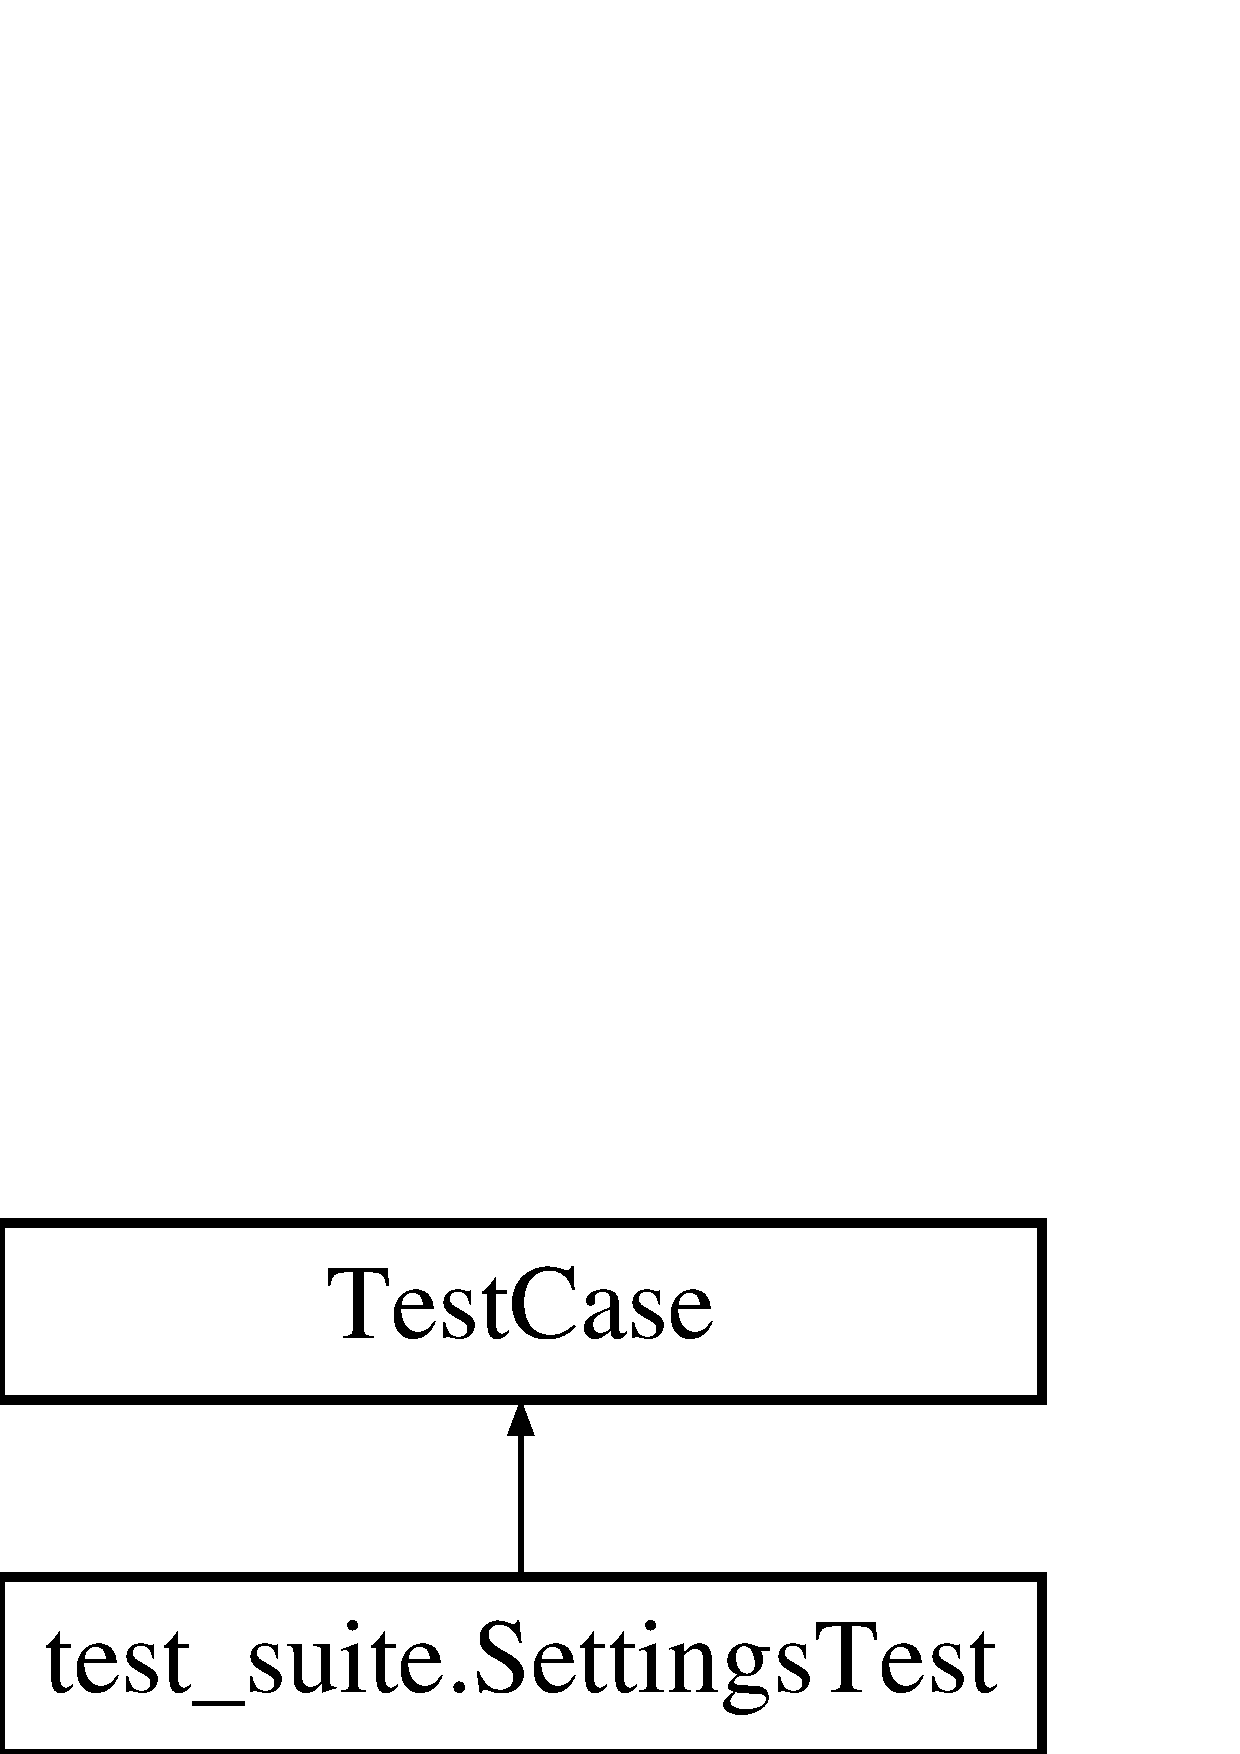
\includegraphics[height=2.000000cm]{classtest__suite_1_1SettingsTest}
\end{center}
\end{figure}
\subsection*{Public Member Functions}
\begin{DoxyCompactItemize}
\item 
\hypertarget{classtest__suite_1_1SettingsTest_aeaf8c43fc51455f8d8ab9d08dfc83fc2}{def {\bfseries set\+Up}}\label{classtest__suite_1_1SettingsTest_aeaf8c43fc51455f8d8ab9d08dfc83fc2}

\end{DoxyCompactItemize}
\subsection*{Public Attributes}
\begin{DoxyCompactItemize}
\item 
\hypertarget{classtest__suite_1_1SettingsTest_aa5ba18125ff41b7c4e906a92da7e47a0}{{\bfseries app}}\label{classtest__suite_1_1SettingsTest_aa5ba18125ff41b7c4e906a92da7e47a0}

\item 
\hypertarget{classtest__suite_1_1SettingsTest_acb4e8a196242a0a395d7777529de431c}{{\bfseries task\+\_\+bar}}\label{classtest__suite_1_1SettingsTest_acb4e8a196242a0a395d7777529de431c}

\end{DoxyCompactItemize}


\subsection{Detailed Description}
\begin{DoxyVerb}Test the settings object.
\end{DoxyVerb}
 

The documentation for this class was generated from the following file\+:\begin{DoxyCompactItemize}
\item 
docs/extensions/extension\+\_\+template/test\+\_\+suite.\+py\end{DoxyCompactItemize}

\hypertarget{classcommotion__client_1_1utils_1_1single__application_1_1SingleApplication}{\section{commotion\+\_\+client.\+utils.\+single\+\_\+application.\+Single\+Application Class Reference}
\label{classcommotion__client_1_1utils_1_1single__application_1_1SingleApplication}\index{commotion\+\_\+client.\+utils.\+single\+\_\+application.\+Single\+Application@{commotion\+\_\+client.\+utils.\+single\+\_\+application.\+Single\+Application}}
}
Inheritance diagram for commotion\+\_\+client.\+utils.\+single\+\_\+application.\+Single\+Application\+:\begin{figure}[H]
\begin{center}
\leavevmode
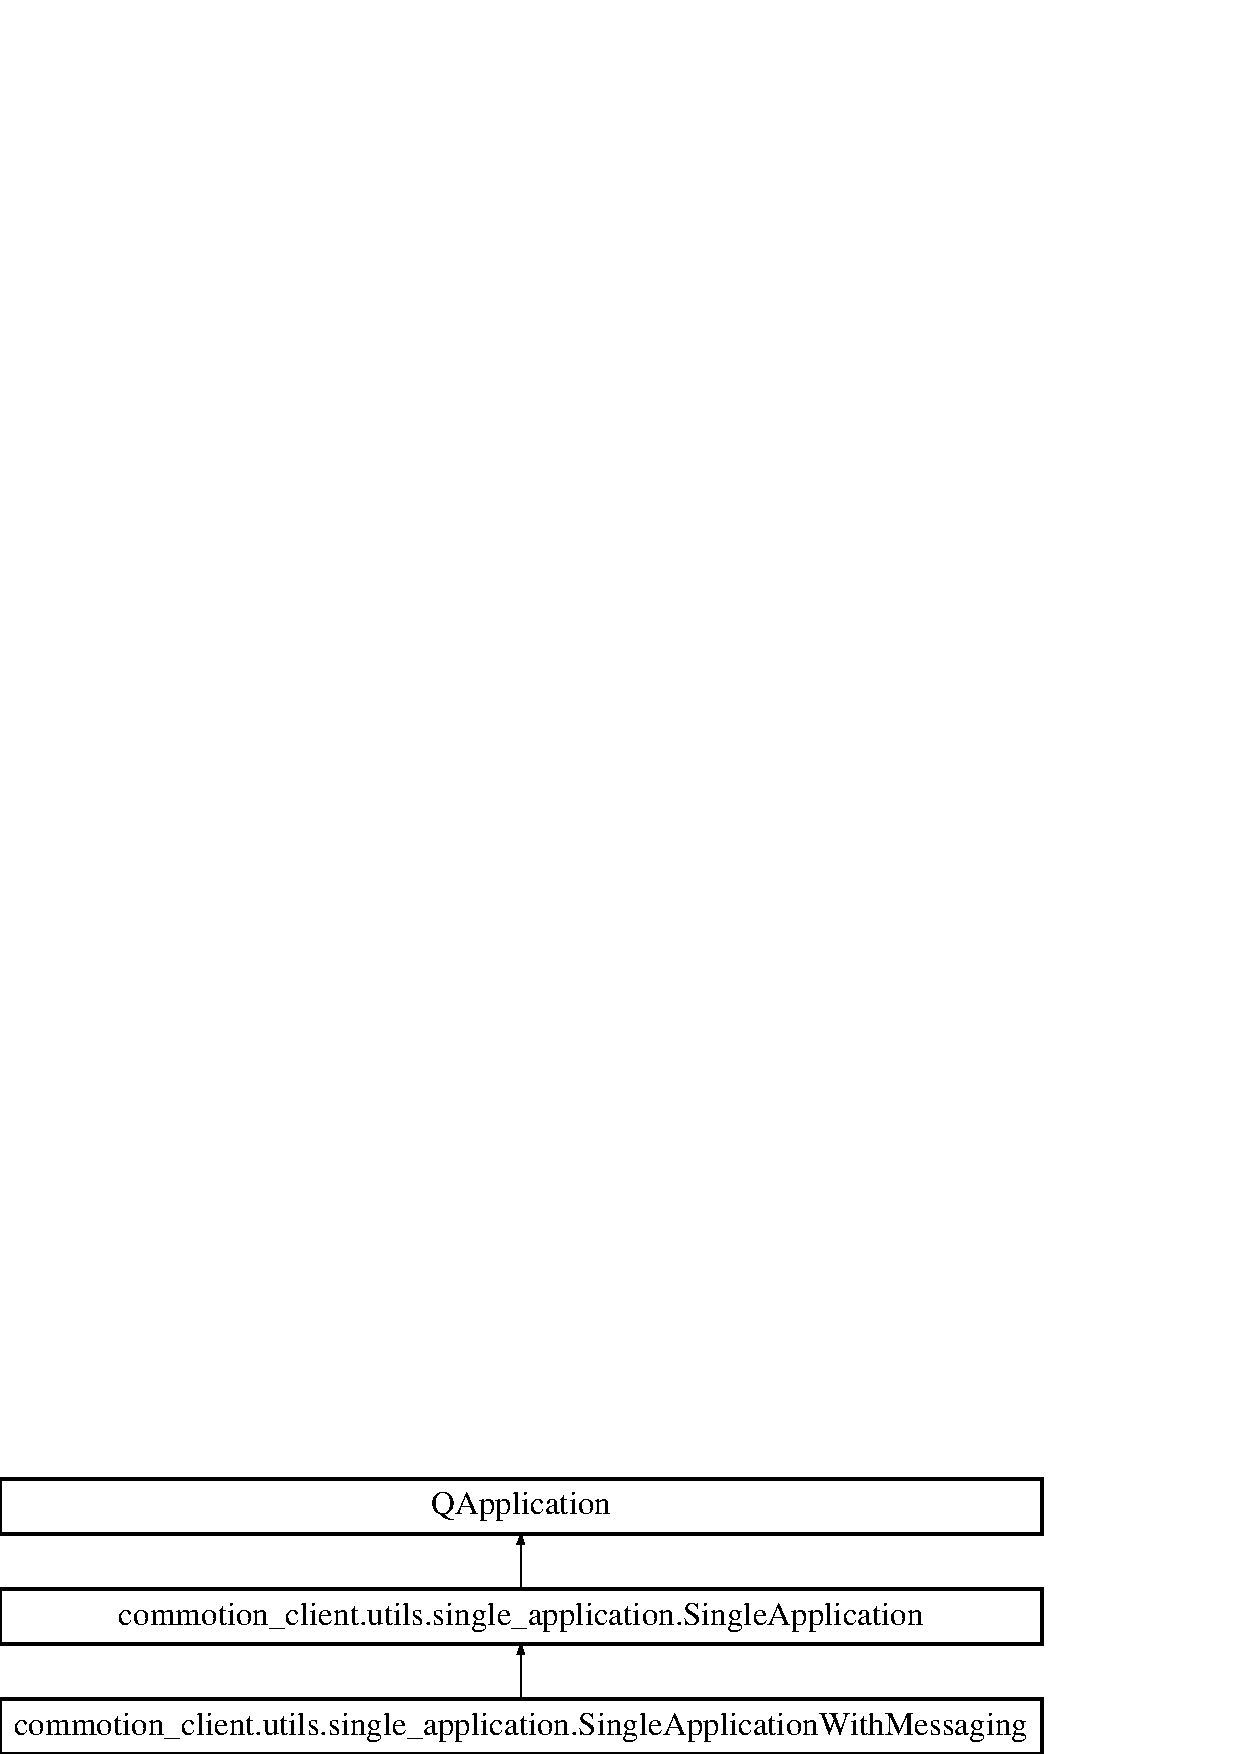
\includegraphics[height=3.000000cm]{classcommotion__client_1_1utils_1_1single__application_1_1SingleApplication}
\end{center}
\end{figure}
\subsection*{Public Member Functions}
\begin{DoxyCompactItemize}
\item 
\hypertarget{classcommotion__client_1_1utils_1_1single__application_1_1SingleApplication_a5d403bbba596b540b6ecb580205111b5}{def {\bfseries \+\_\+\+\_\+init\+\_\+\+\_\+}}\label{classcommotion__client_1_1utils_1_1single__application_1_1SingleApplication_a5d403bbba596b540b6ecb580205111b5}

\item 
\hypertarget{classcommotion__client_1_1utils_1_1single__application_1_1SingleApplication_acf757577a5b8729d162c828275e1b948}{def {\bfseries is\+\_\+running}}\label{classcommotion__client_1_1utils_1_1single__application_1_1SingleApplication_acf757577a5b8729d162c828275e1b948}

\end{DoxyCompactItemize}
\subsection*{Public Attributes}
\begin{DoxyCompactItemize}
\item 
\hypertarget{classcommotion__client_1_1utils_1_1single__application_1_1SingleApplication_a0d42a4c04a6fc8df6522699695110c2b}{{\bfseries log}}\label{classcommotion__client_1_1utils_1_1single__application_1_1SingleApplication_a0d42a4c04a6fc8df6522699695110c2b}

\item 
\hypertarget{classcommotion__client_1_1utils_1_1single__application_1_1SingleApplication_a1aceece78c1e408d8d94ed8764f246a4}{{\bfseries main}}\label{classcommotion__client_1_1utils_1_1single__application_1_1SingleApplication_a1aceece78c1e408d8d94ed8764f246a4}

\item 
\hypertarget{classcommotion__client_1_1utils_1_1single__application_1_1SingleApplication_ae4582c8bf029813714440ea61ef77b3d}{{\bfseries status\+\_\+bar}}\label{classcommotion__client_1_1utils_1_1single__application_1_1SingleApplication_ae4582c8bf029813714440ea61ef77b3d}

\item 
\hypertarget{classcommotion__client_1_1utils_1_1single__application_1_1SingleApplication_adbe8eec2bb7d760cb6f39fd03957f8f6}{{\bfseries control\+\_\+panel}}\label{classcommotion__client_1_1utils_1_1single__application_1_1SingleApplication_adbe8eec2bb7d760cb6f39fd03957f8f6}

\item 
\hypertarget{classcommotion__client_1_1utils_1_1single__application_1_1SingleApplication_ae2b4a1243e937e06fef4cf521cc5cca5}{{\bfseries shared\+\_\+memory}}\label{classcommotion__client_1_1utils_1_1single__application_1_1SingleApplication_ae2b4a1243e937e06fef4cf521cc5cca5}

\end{DoxyCompactItemize}


\subsection{Detailed Description}
\begin{DoxyVerb}Single application instance uses a key and shared memory to ensure that only one instance of the Commotion client is ever running at the same time.
\end{DoxyVerb}
 

The documentation for this class was generated from the following file\+:\begin{DoxyCompactItemize}
\item 
commotion\+\_\+client/utils/single\+\_\+application.\+py\end{DoxyCompactItemize}

\hypertarget{classcommotion__client_1_1utils_1_1single__application_1_1SingleApplicationWithMessaging}{\section{commotion\-\_\-client.\-utils.\-single\-\_\-application.\-Single\-Application\-With\-Messaging Class Reference}
\label{classcommotion__client_1_1utils_1_1single__application_1_1SingleApplicationWithMessaging}\index{commotion\-\_\-client.\-utils.\-single\-\_\-application.\-Single\-Application\-With\-Messaging@{commotion\-\_\-client.\-utils.\-single\-\_\-application.\-Single\-Application\-With\-Messaging}}
}
Inheritance diagram for commotion\-\_\-client.\-utils.\-single\-\_\-application.\-Single\-Application\-With\-Messaging\-:\begin{figure}[H]
\begin{center}
\leavevmode
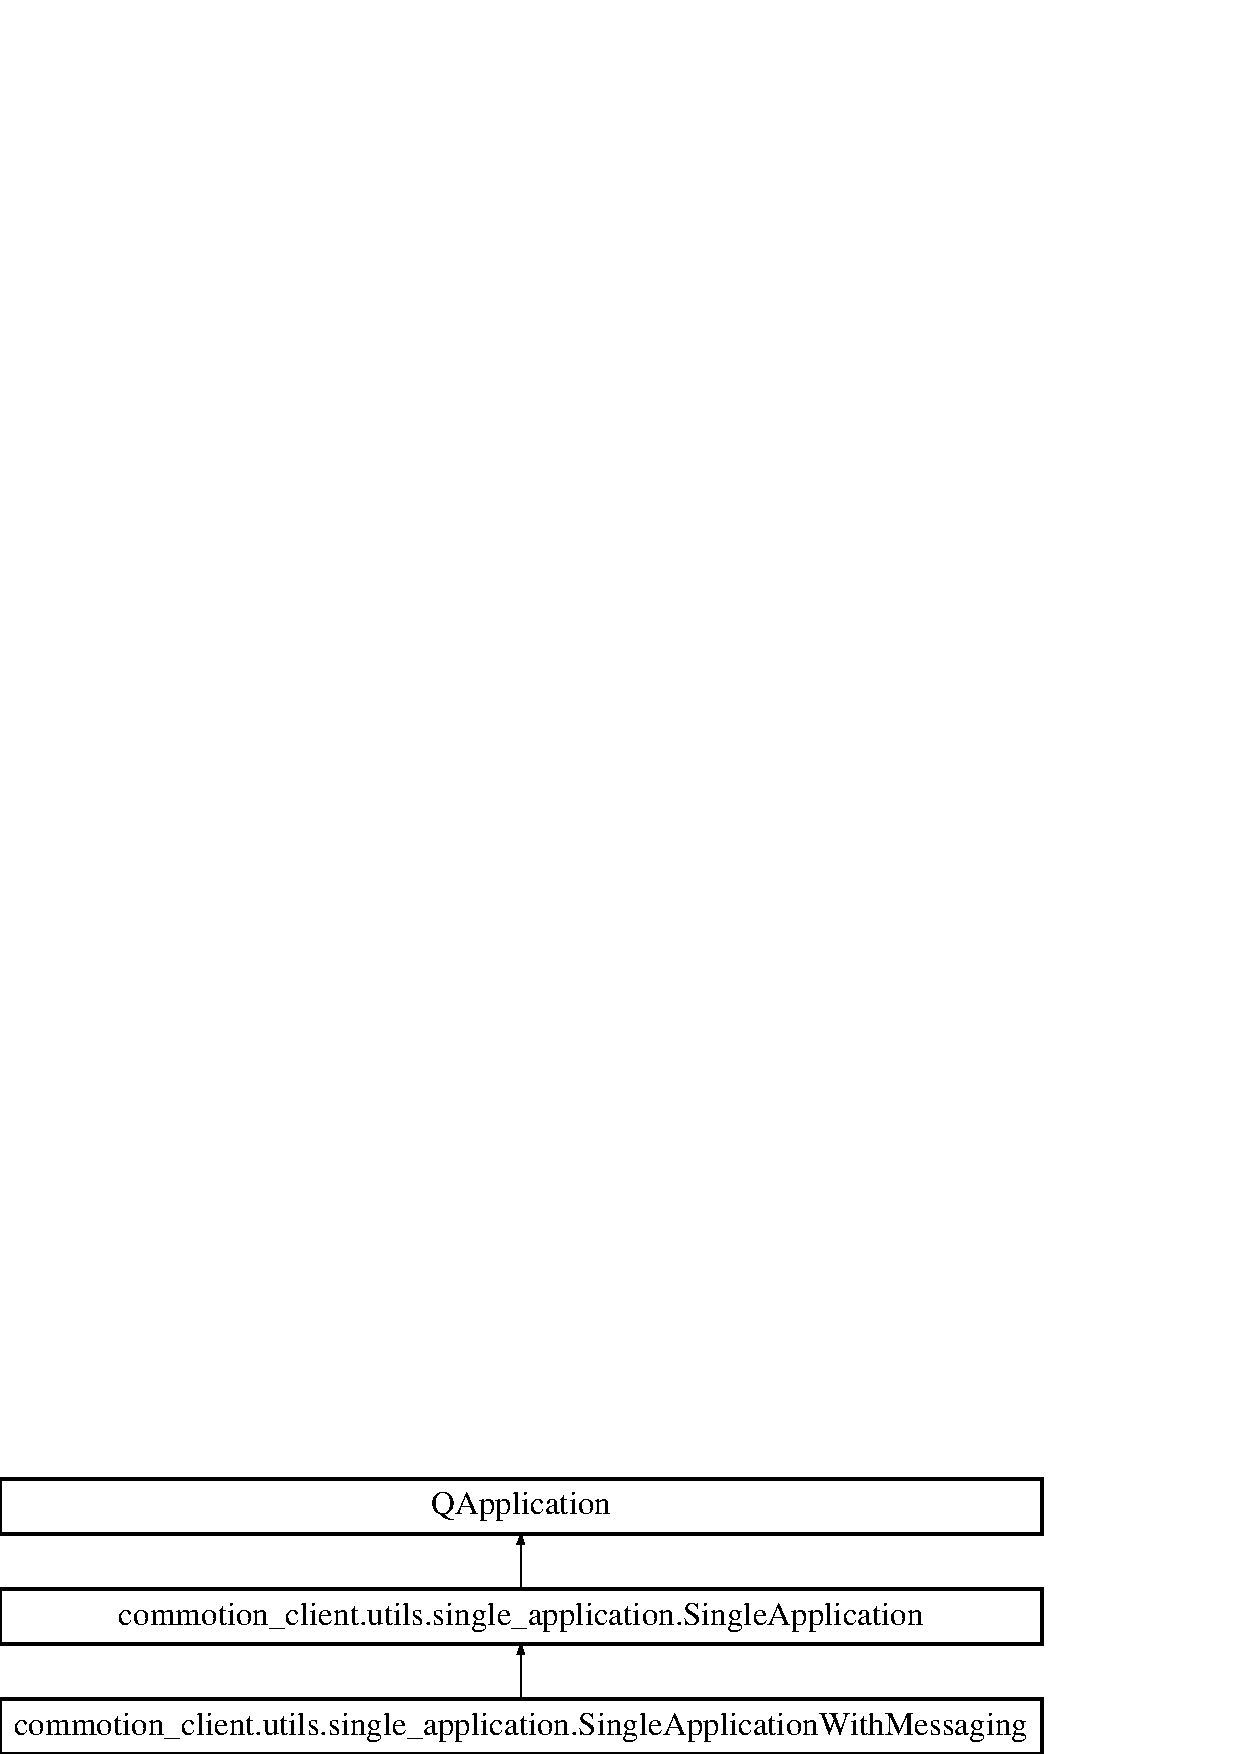
\includegraphics[height=3.000000cm]{classcommotion__client_1_1utils_1_1single__application_1_1SingleApplicationWithMessaging}
\end{center}
\end{figure}
\subsection*{Public Member Functions}
\begin{DoxyCompactItemize}
\item 
\hypertarget{classcommotion__client_1_1utils_1_1single__application_1_1SingleApplicationWithMessaging_a267f94646304f99b18a0ade20db51d80}{def {\bfseries \-\_\-\-\_\-init\-\_\-\-\_\-}}\label{classcommotion__client_1_1utils_1_1single__application_1_1SingleApplicationWithMessaging_a267f94646304f99b18a0ade20db51d80}

\item 
def \hyperlink{classcommotion__client_1_1utils_1_1single__application_1_1SingleApplicationWithMessaging_a1289d2bf53f8a3647dd9bce62bd877e6}{handle\-\_\-message}
\item 
def \hyperlink{classcommotion__client_1_1utils_1_1single__application_1_1SingleApplicationWithMessaging_a07475e0643ef2f92a0e990e7feefa4e3}{send\-\_\-message}
\item 
def \hyperlink{classcommotion__client_1_1utils_1_1single__application_1_1SingleApplicationWithMessaging_af0bf77fe13d6cd9e27d13927f4dcaae4}{process\-\_\-message}
\end{DoxyCompactItemize}
\subsection*{Additional Inherited Members}


\subsection{Detailed Description}
\begin{DoxyVerb}The interprocess messaging class for the Commotion Client. This class extends the single application to allow for instantiations of the Commotion Client to pass messages to the existing client if it is already running. When a second instance of a Commotion Client is run without a message specified it will reaise the earler clients main window to the front and then close itself.

e.g:
python3.3 CommotionClient.py --message "COMMAND"
\end{DoxyVerb}
 

\subsection{Member Function Documentation}
\hypertarget{classcommotion__client_1_1utils_1_1single__application_1_1SingleApplicationWithMessaging_a1289d2bf53f8a3647dd9bce62bd877e6}{\index{commotion\-\_\-client\-::utils\-::single\-\_\-application\-::\-Single\-Application\-With\-Messaging@{commotion\-\_\-client\-::utils\-::single\-\_\-application\-::\-Single\-Application\-With\-Messaging}!handle\-\_\-message@{handle\-\_\-message}}
\index{handle\-\_\-message@{handle\-\_\-message}!commotion_client::utils::single_application::SingleApplicationWithMessaging@{commotion\-\_\-client\-::utils\-::single\-\_\-application\-::\-Single\-Application\-With\-Messaging}}
\subsubsection[{handle\-\_\-message}]{\setlength{\rightskip}{0pt plus 5cm}def commotion\-\_\-client.\-utils.\-single\-\_\-application.\-Single\-Application\-With\-Messaging.\-handle\-\_\-message (
\begin{DoxyParamCaption}
\item[{}]{self}
\end{DoxyParamCaption}
)}}\label{classcommotion__client_1_1utils_1_1single__application_1_1SingleApplicationWithMessaging_a1289d2bf53f8a3647dd9bce62bd877e6}
\begin{DoxyVerb}Server side implementation of the messaging functions. This function waits for signals it receives and then emits a SIGNAL "messageAvailable" with the decoded message.

(Emits a signal instead of just calling a function in case we decide we would like to allow other components or extensions to listen for messages from new instances.)
\end{DoxyVerb}
 

References commotion\-\_\-client.\-utils.\-single\-\_\-application.\-Single\-Application\-With\-Messaging.\-\_\-timeout, commotion\-\_\-client.\-G\-U\-I.\-menu\-\_\-bar.\-Menu\-Bar.\-translate, commotion\-\_\-client.\-extensions.\-config\-\_\-editor.\-main.\-View\-Port.\-translate, commotion\-\_\-client.\-G\-U\-I.\-main\-\_\-window.\-Main\-Window.\-translate, commotion\-\_\-client.\-G\-U\-I.\-toolbar\-\_\-builder.\-Tool\-Bar.\-translate, commotion\-\_\-client.\-G\-U\-I.\-extension\-\_\-toolbar.\-Extension\-Tool\-Bar.\-translate, commotion\-\_\-client.\-G\-U\-I.\-toolbar.\-Tool\-Bar.\-translate, commotion\-\_\-client.\-utils.\-validate.\-Client\-Config.\-translate, commotion\-\_\-client.\-utils.\-extension\-\_\-manager.\-Extension\-Manager.\-translate, commotion\-\_\-client.\-G\-U\-I.\-extension\-\_\-toolbar.\-Menu\-Item.\-translate, commotion\-\_\-client.\-commotion\-\_\-client.\-Commotion\-Client\-Application.\-translate, commotion\-\_\-client.\-utils.\-validate.\-Networking.\-translate, and commotion\-\_\-client.\-utils.\-extension\-\_\-manager.\-Config\-Manager.\-translate.


\begin{DoxyCode}
76 
77     \textcolor{keyword}{def }\hyperlink{classcommotion__client_1_1utils_1_1single__application_1_1SingleApplicationWithMessaging_a1289d2bf53f8a3647dd9bce62bd877e6}{handle\_message}(self):
78         \textcolor{stringliteral}{"""}
79 \textcolor{stringliteral}{        Server side implementation of the messaging functions. This function waits for signals it receives
       and then emits a SIGNAL "messageAvailable" with the decoded message.}
80 \textcolor{stringliteral}{        }
81 \textcolor{stringliteral}{        (Emits a signal instead of just calling a function in case we decide we would like to allow other
       components or extensions to listen for messages from new instances.)}
82 \textcolor{stringliteral}{        """}
83         socket = self.\_server.nextPendingConnection()
84         \textcolor{keywordflow}{if} socket.waitForReadyRead(self.\hyperlink{classcommotion__client_1_1utils_1_1single__application_1_1SingleApplicationWithMessaging_ae4ca7cb1d3bf9e9ebc683c953c8c08f4}{\_timeout}):
85             self.emit(QtCore.SIGNAL(\textcolor{stringliteral}{"messageAvailable"}), bytes(socket.readAll().data()).decode(\textcolor{stringliteral}{'utf-8'}))
86             socket.disconnectFromServer()
87             self.log.debug(self.translate(\textcolor{stringliteral}{"logs"}, \textcolor{stringliteral}{"message received and emitted in a messageAvailable
       signal"}))
88         \textcolor{keywordflow}{else}:
89             self.log.error(socket.errorString())

\end{DoxyCode}
\hypertarget{classcommotion__client_1_1utils_1_1single__application_1_1SingleApplicationWithMessaging_af0bf77fe13d6cd9e27d13927f4dcaae4}{\index{commotion\-\_\-client\-::utils\-::single\-\_\-application\-::\-Single\-Application\-With\-Messaging@{commotion\-\_\-client\-::utils\-::single\-\_\-application\-::\-Single\-Application\-With\-Messaging}!process\-\_\-message@{process\-\_\-message}}
\index{process\-\_\-message@{process\-\_\-message}!commotion_client::utils::single_application::SingleApplicationWithMessaging@{commotion\-\_\-client\-::utils\-::single\-\_\-application\-::\-Single\-Application\-With\-Messaging}}
\subsubsection[{process\-\_\-message}]{\setlength{\rightskip}{0pt plus 5cm}def commotion\-\_\-client.\-utils.\-single\-\_\-application.\-Single\-Application\-With\-Messaging.\-process\-\_\-message (
\begin{DoxyParamCaption}
\item[{}]{self, }
\item[{}]{message}
\end{DoxyParamCaption}
)}}\label{classcommotion__client_1_1utils_1_1single__application_1_1SingleApplicationWithMessaging_af0bf77fe13d6cd9e27d13927f4dcaae4}
\begin{DoxyVerb}Process which processes messages an app receives and takes actions on valid requests.
\end{DoxyVerb}
 

References commotion\-\_\-client.\-G\-U\-I.\-menu\-\_\-bar.\-Menu\-Bar.\-translate, commotion\-\_\-client.\-extensions.\-config\-\_\-editor.\-main.\-View\-Port.\-translate, commotion\-\_\-client.\-G\-U\-I.\-main\-\_\-window.\-Main\-Window.\-translate, commotion\-\_\-client.\-G\-U\-I.\-toolbar\-\_\-builder.\-Tool\-Bar.\-translate, commotion\-\_\-client.\-utils.\-validate.\-Client\-Config.\-translate, commotion\-\_\-client.\-G\-U\-I.\-extension\-\_\-toolbar.\-Extension\-Tool\-Bar.\-translate, commotion\-\_\-client.\-G\-U\-I.\-toolbar.\-Tool\-Bar.\-translate, commotion\-\_\-client.\-utils.\-extension\-\_\-manager.\-Extension\-Manager.\-translate, commotion\-\_\-client.\-G\-U\-I.\-extension\-\_\-toolbar.\-Menu\-Item.\-translate, commotion\-\_\-client.\-commotion\-\_\-client.\-Commotion\-Client\-Application.\-translate, commotion\-\_\-client.\-utils.\-validate.\-Networking.\-translate, and commotion\-\_\-client.\-utils.\-extension\-\_\-manager.\-Config\-Manager.\-translate.


\begin{DoxyCode}
109 
110     \textcolor{keyword}{def }\hyperlink{classcommotion__client_1_1utils_1_1single__application_1_1SingleApplicationWithMessaging_af0bf77fe13d6cd9e27d13927f4dcaae4}{process\_message}(self, message):
111         \textcolor{stringliteral}{"""}
112 \textcolor{stringliteral}{        Process which processes messages an app receives and takes actions on valid requests.}
113 \textcolor{stringliteral}{        """}
114         self.log.debug(self.translate(\textcolor{stringliteral}{"logs"}, \textcolor{stringliteral}{"Applicaiton received a message \{0\}, but does not have a
       message parser to handle it."}).format(message))
\end{DoxyCode}
\hypertarget{classcommotion__client_1_1utils_1_1single__application_1_1SingleApplicationWithMessaging_a07475e0643ef2f92a0e990e7feefa4e3}{\index{commotion\-\_\-client\-::utils\-::single\-\_\-application\-::\-Single\-Application\-With\-Messaging@{commotion\-\_\-client\-::utils\-::single\-\_\-application\-::\-Single\-Application\-With\-Messaging}!send\-\_\-message@{send\-\_\-message}}
\index{send\-\_\-message@{send\-\_\-message}!commotion_client::utils::single_application::SingleApplicationWithMessaging@{commotion\-\_\-client\-::utils\-::single\-\_\-application\-::\-Single\-Application\-With\-Messaging}}
\subsubsection[{send\-\_\-message}]{\setlength{\rightskip}{0pt plus 5cm}def commotion\-\_\-client.\-utils.\-single\-\_\-application.\-Single\-Application\-With\-Messaging.\-send\-\_\-message (
\begin{DoxyParamCaption}
\item[{}]{self, }
\item[{}]{message}
\end{DoxyParamCaption}
)}}\label{classcommotion__client_1_1utils_1_1single__application_1_1SingleApplicationWithMessaging_a07475e0643ef2f92a0e990e7feefa4e3}
\begin{DoxyVerb}Message sending function. Connected to local socket specified by shared key and if successful writes the message to it and returns.
\end{DoxyVerb}
 

References commotion\-\_\-client.\-utils.\-single\-\_\-application.\-Single\-Application.\-\_\-key, commotion\-\_\-client.\-utils.\-single\-\_\-application.\-Single\-Application\-With\-Messaging.\-\_\-timeout, commotion\-\_\-client.\-utils.\-single\-\_\-application.\-Single\-Application.\-is\-\_\-running(), commotion\-\_\-client.\-G\-U\-I.\-menu\-\_\-bar.\-Menu\-Bar.\-translate, commotion\-\_\-client.\-extensions.\-config\-\_\-editor.\-main.\-View\-Port.\-translate, commotion\-\_\-client.\-G\-U\-I.\-main\-\_\-window.\-Main\-Window.\-translate, commotion\-\_\-client.\-G\-U\-I.\-toolbar\-\_\-builder.\-Tool\-Bar.\-translate, commotion\-\_\-client.\-G\-U\-I.\-toolbar.\-Tool\-Bar.\-translate, commotion\-\_\-client.\-G\-U\-I.\-extension\-\_\-toolbar.\-Extension\-Tool\-Bar.\-translate, commotion\-\_\-client.\-utils.\-validate.\-Client\-Config.\-translate, commotion\-\_\-client.\-utils.\-extension\-\_\-manager.\-Extension\-Manager.\-translate, commotion\-\_\-client.\-G\-U\-I.\-extension\-\_\-toolbar.\-Menu\-Item.\-translate, commotion\-\_\-client.\-commotion\-\_\-client.\-Commotion\-Client\-Application.\-translate, commotion\-\_\-client.\-utils.\-validate.\-Networking.\-translate, and commotion\-\_\-client.\-utils.\-extension\-\_\-manager.\-Config\-Manager.\-translate.


\begin{DoxyCode}
90 
91     \textcolor{keyword}{def }\hyperlink{classcommotion__client_1_1utils_1_1single__application_1_1SingleApplicationWithMessaging_a07475e0643ef2f92a0e990e7feefa4e3}{send\_message}(self, message):
92         \textcolor{stringliteral}{"""}
93 \textcolor{stringliteral}{        Message sending function. Connected to local socket specified by shared key and if successful
       writes the message to it and returns.}
94 \textcolor{stringliteral}{        """}
95         \textcolor{keywordflow}{if} self.\hyperlink{classcommotion__client_1_1utils_1_1single__application_1_1SingleApplication_acf757577a5b8729d162c828275e1b948}{is\_running}():
96             socket = QtNetwork.QLocalSocket(self)
97             socket.connectToServer(self.\hyperlink{classcommotion__client_1_1utils_1_1single__application_1_1SingleApplication_a9c95e184472415ffd42cb82dcf14a332}{\_key}, QtCore.QIODevice.WriteOnly)
98             \textcolor{keywordflow}{if} \textcolor{keywordflow}{not} socket.waitForConnected(self.\hyperlink{classcommotion__client_1_1utils_1_1single__application_1_1SingleApplicationWithMessaging_ae4ca7cb1d3bf9e9ebc683c953c8c08f4}{\_timeout}):
99                 self.log.error(socket.errorString())
100                 \textcolor{keywordflow}{return} \textcolor{keyword}{False}
101             socket.write(str(message).encode(\textcolor{stringliteral}{"utf-8"}))
102             \textcolor{keywordflow}{if} \textcolor{keywordflow}{not} socket.waitForBytesWritten(self.\hyperlink{classcommotion__client_1_1utils_1_1single__application_1_1SingleApplicationWithMessaging_ae4ca7cb1d3bf9e9ebc683c953c8c08f4}{\_timeout}):
103                 self.log.error(socket.errorString())
104                 \textcolor{keywordflow}{return} \textcolor{keyword}{False}
105             socket.disconnectFromServer()
106             \textcolor{keywordflow}{return} \textcolor{keyword}{True}
107         self.log.debug(self.translate(\textcolor{stringliteral}{"logs"}, \textcolor{stringliteral}{"Attempted to send message when commotion client application
       was not currently running."}))
108         \textcolor{keywordflow}{return} \textcolor{keyword}{False}

\end{DoxyCode}


The documentation for this class was generated from the following file\-:\begin{DoxyCompactItemize}
\item 
commotion\-\_\-client/utils/single\-\_\-application.\-py\end{DoxyCompactItemize}

\hypertarget{classcommotion__client_1_1GUI_1_1menu__bar_1_1subMenuWidget}{\section{commotion\+\_\+client.\+G\+U\+I.\+menu\+\_\+bar.\+sub\+Menu\+Widget Class Reference}
\label{classcommotion__client_1_1GUI_1_1menu__bar_1_1subMenuWidget}\index{commotion\+\_\+client.\+G\+U\+I.\+menu\+\_\+bar.\+sub\+Menu\+Widget@{commotion\+\_\+client.\+G\+U\+I.\+menu\+\_\+bar.\+sub\+Menu\+Widget}}
}
Inheritance diagram for commotion\+\_\+client.\+G\+U\+I.\+menu\+\_\+bar.\+sub\+Menu\+Widget\+:\begin{figure}[H]
\begin{center}
\leavevmode
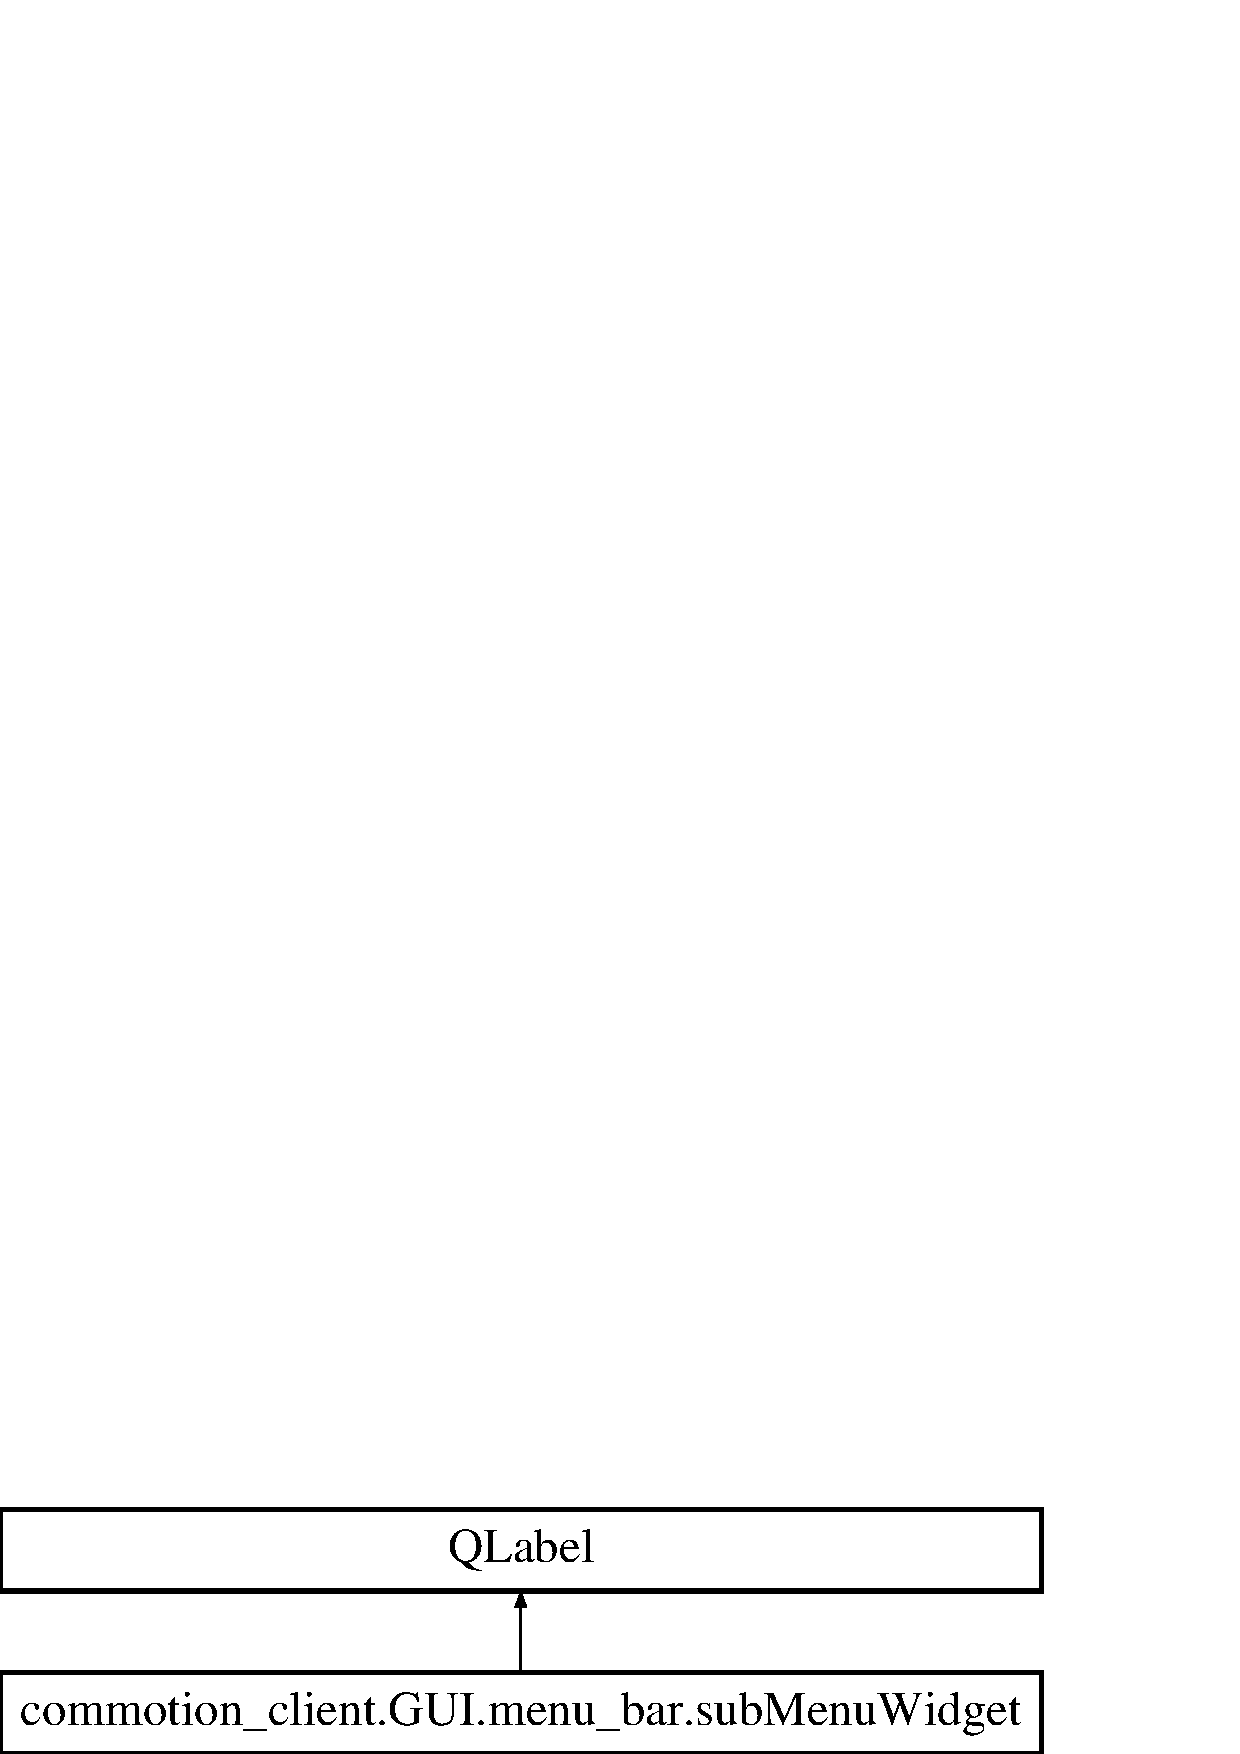
\includegraphics[height=2.000000cm]{classcommotion__client_1_1GUI_1_1menu__bar_1_1subMenuWidget}
\end{center}
\end{figure}
\subsection*{Public Member Functions}
\begin{DoxyCompactItemize}
\item 
\hypertarget{classcommotion__client_1_1GUI_1_1menu__bar_1_1subMenuWidget_adfb72c16f79d60a460836f368d636867}{def {\bfseries \+\_\+\+\_\+init\+\_\+\+\_\+}}\label{classcommotion__client_1_1GUI_1_1menu__bar_1_1subMenuWidget_adfb72c16f79d60a460836f368d636867}

\item 
\hypertarget{classcommotion__client_1_1GUI_1_1menu__bar_1_1subMenuWidget_a360c7df2bc1675f2eacc63ed076fba6f}{def {\bfseries mouse\+Release\+Event}}\label{classcommotion__client_1_1GUI_1_1menu__bar_1_1subMenuWidget_a360c7df2bc1675f2eacc63ed076fba6f}

\end{DoxyCompactItemize}
\subsection*{Static Public Attributes}
\begin{DoxyCompactItemize}
\item 
\hypertarget{classcommotion__client_1_1GUI_1_1menu__bar_1_1subMenuWidget_a9d362f09bf58710e2d5cc3299f20852c}{tuple {\bfseries clicked} = Qt\+Core.\+pyqt\+Signal()}\label{classcommotion__client_1_1GUI_1_1menu__bar_1_1subMenuWidget_a9d362f09bf58710e2d5cc3299f20852c}

\end{DoxyCompactItemize}


\subsection{Detailed Description}
\begin{DoxyVerb}This class extends QLabel to make clickable labels.
\end{DoxyVerb}
 

The documentation for this class was generated from the following file\+:\begin{DoxyCompactItemize}
\item 
commotion\+\_\+client/\+G\+U\+I/menu\+\_\+bar.\+py\end{DoxyCompactItemize}

\hypertarget{classtask__bar_1_1TaskBar}{\section{task\+\_\+bar.\+Task\+Bar Class Reference}
\label{classtask__bar_1_1TaskBar}\index{task\+\_\+bar.\+Task\+Bar@{task\+\_\+bar.\+Task\+Bar}}
}


\subsection{Detailed Description}
\begin{DoxyVerb}\end{DoxyVerb}
 

The documentation for this class was generated from the following file\+:\begin{DoxyCompactItemize}
\item 
docs/extensions/extension\+\_\+template/task\+\_\+bar.\+py\end{DoxyCompactItemize}

\hypertarget{classtest__suite_1_1TaskBarTest}{\section{test\-\_\-suite.\-Task\-Bar\-Test Class Reference}
\label{classtest__suite_1_1TaskBarTest}\index{test\-\_\-suite.\-Task\-Bar\-Test@{test\-\_\-suite.\-Task\-Bar\-Test}}
}
Inheritance diagram for test\-\_\-suite.\-Task\-Bar\-Test\-:\begin{figure}[H]
\begin{center}
\leavevmode
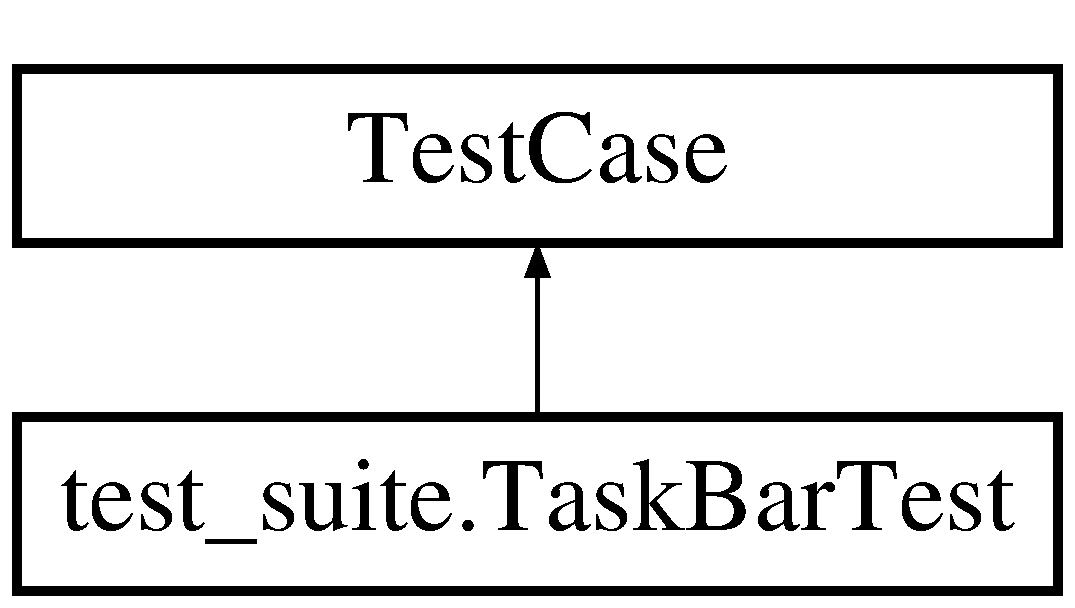
\includegraphics[height=2.000000cm]{classtest__suite_1_1TaskBarTest}
\end{center}
\end{figure}
\subsection*{Public Member Functions}
\begin{DoxyCompactItemize}
\item 
\hypertarget{classtest__suite_1_1TaskBarTest_a4fb9a558b494482ea7a27aba20cac5c7}{def {\bfseries set\-Up}}\label{classtest__suite_1_1TaskBarTest_a4fb9a558b494482ea7a27aba20cac5c7}

\end{DoxyCompactItemize}
\subsection*{Public Attributes}
\begin{DoxyCompactItemize}
\item 
\hypertarget{classtest__suite_1_1TaskBarTest_ad53e0ba8e35387cfb615483b7f898972}{{\bfseries app}}\label{classtest__suite_1_1TaskBarTest_ad53e0ba8e35387cfb615483b7f898972}

\item 
\hypertarget{classtest__suite_1_1TaskBarTest_a65d36a754a8278c6c572b32d92628686}{{\bfseries task\-\_\-bar}}\label{classtest__suite_1_1TaskBarTest_a65d36a754a8278c6c572b32d92628686}

\end{DoxyCompactItemize}


\subsection{Detailed Description}
\begin{DoxyVerb}Test the task bar object
\end{DoxyVerb}
 

The documentation for this class was generated from the following file\-:\begin{DoxyCompactItemize}
\item 
docs/extensions/extension\-\_\-template/test\-\_\-suite.\-py\end{DoxyCompactItemize}

\hypertarget{classcommotion__client_1_1GUI_1_1toolbar__builder_1_1ToolBar}{\section{commotion\+\_\+client.\+G\+U\+I.\+toolbar\+\_\+builder.\+Tool\+Bar Class Reference}
\label{classcommotion__client_1_1GUI_1_1toolbar__builder_1_1ToolBar}\index{commotion\+\_\+client.\+G\+U\+I.\+toolbar\+\_\+builder.\+Tool\+Bar@{commotion\+\_\+client.\+G\+U\+I.\+toolbar\+\_\+builder.\+Tool\+Bar}}
}
Inheritance diagram for commotion\+\_\+client.\+G\+U\+I.\+toolbar\+\_\+builder.\+Tool\+Bar\+:\begin{figure}[H]
\begin{center}
\leavevmode
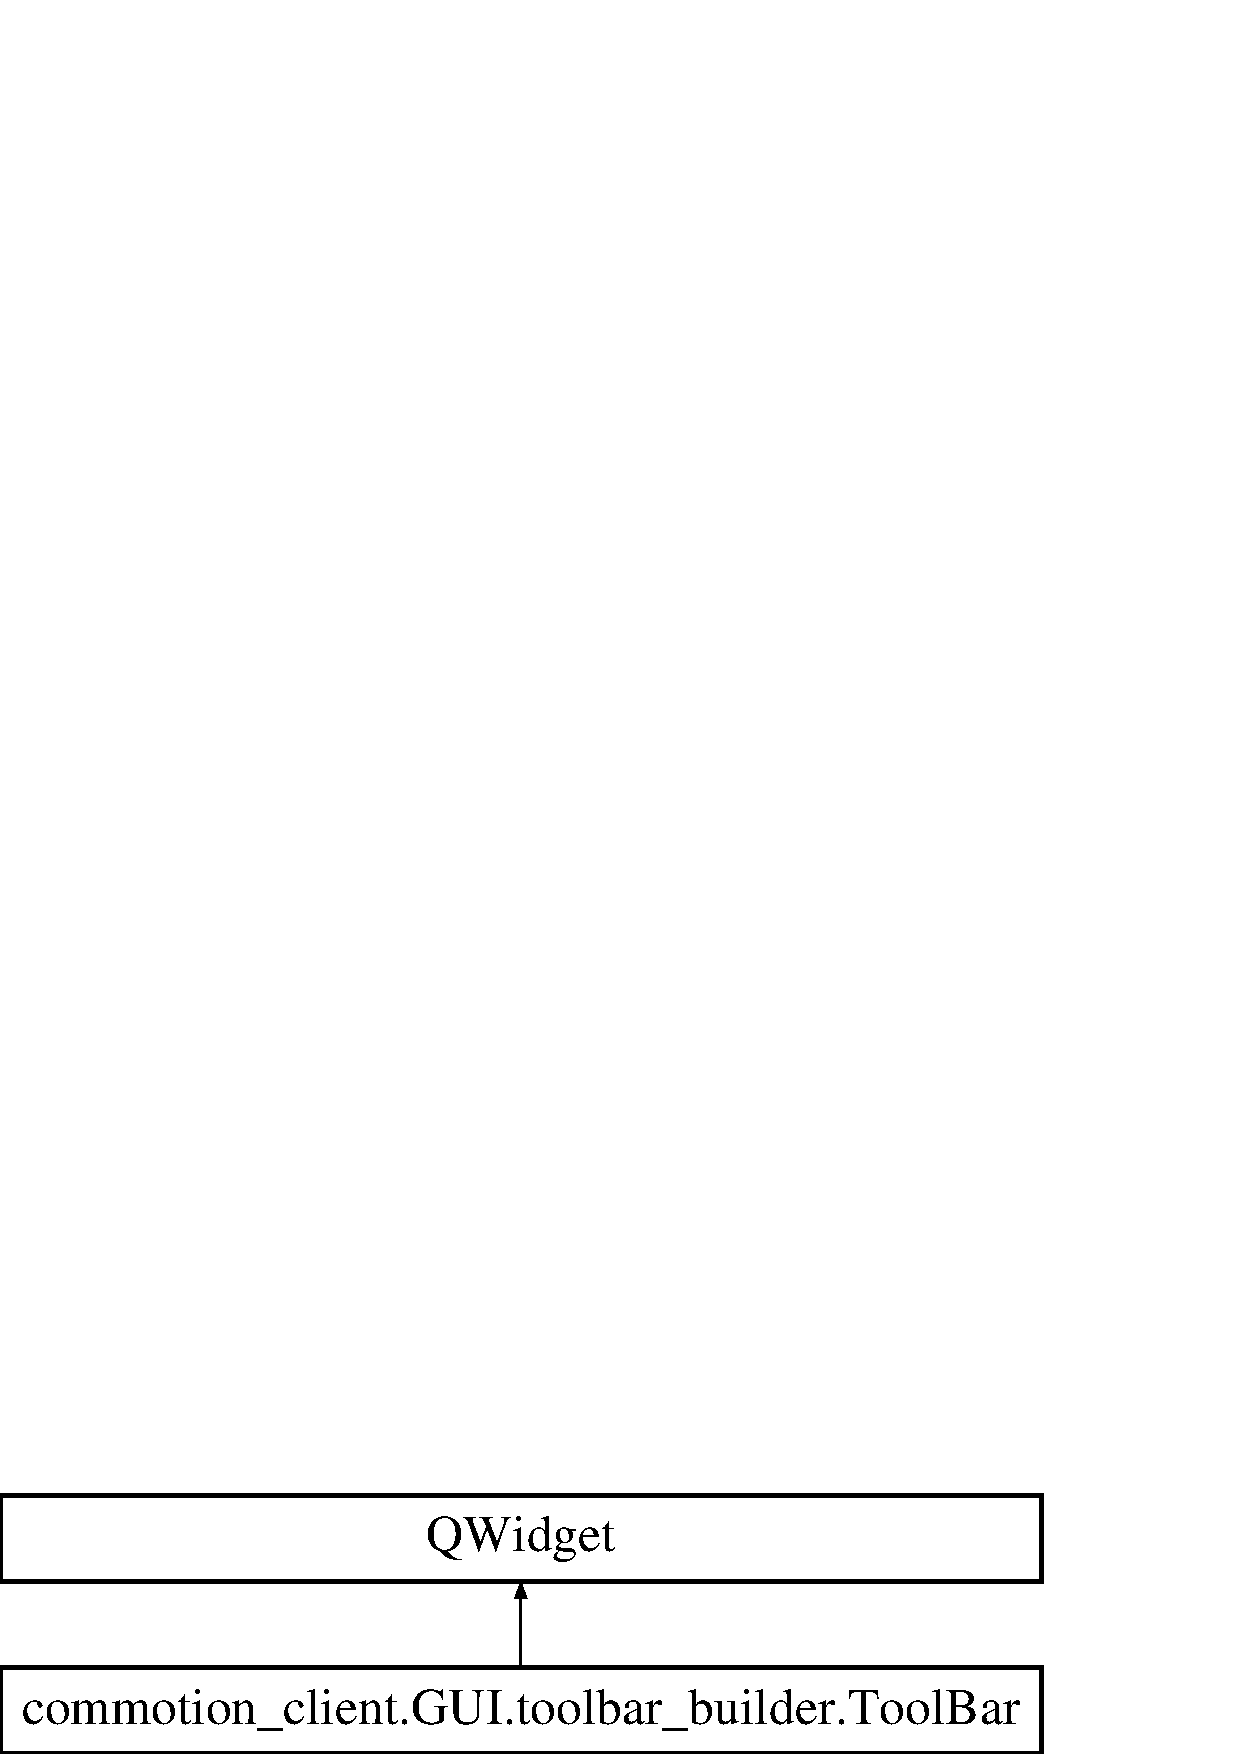
\includegraphics[height=2.000000cm]{classcommotion__client_1_1GUI_1_1toolbar__builder_1_1ToolBar}
\end{center}
\end{figure}
\subsection*{Public Member Functions}
\begin{DoxyCompactItemize}
\item 
def \hyperlink{classcommotion__client_1_1GUI_1_1toolbar__builder_1_1ToolBar_a86bce4db69461426435f4d6876e3e142}{\+\_\+\+\_\+init\+\_\+\+\_\+}
\item 
def \hyperlink{classcommotion__client_1_1GUI_1_1toolbar__builder_1_1ToolBar_a075b6709f65ef1aeaca34c69dd305379}{init\+\_\+settings}
\item 
def \hyperlink{classcommotion__client_1_1GUI_1_1toolbar__builder_1_1ToolBar_ab83f3bd0cdc3c0316dffaf55056c60c1}{load\+\_\+settings}
\item 
def \hyperlink{classcommotion__client_1_1GUI_1_1toolbar__builder_1_1ToolBar_a11640e9ec7f3f4dbc519824f950c6a79}{load\+\_\+about}
\item 
def \hyperlink{classcommotion__client_1_1GUI_1_1toolbar__builder_1_1ToolBar_a7d39c09c09071fba355d238cb6c1ad40}{load\+\_\+update}
\item 
def \hyperlink{classcommotion__client_1_1GUI_1_1toolbar__builder_1_1ToolBar_ad435b7c5d002f1b57e24aa7ee258085c}{load\+\_\+user}
\item 
def \hyperlink{classcommotion__client_1_1GUI_1_1toolbar__builder_1_1ToolBar_acf2126aa2356761e1112b9fa96535b44}{exit\+\_\+application}
\item 
def \hyperlink{classcommotion__client_1_1GUI_1_1toolbar__builder_1_1ToolBar_a0a0d3e80c3d039cfd2cc5d445b06b3c7}{load\+\_\+extensions}
\item 
def \hyperlink{classcommotion__client_1_1GUI_1_1toolbar__builder_1_1ToolBar_acb281187f13361c64835fa443416c8c2}{init\+\_\+user}
\item 
def \hyperlink{classcommotion__client_1_1GUI_1_1toolbar__builder_1_1ToolBar_ad033424f51c9cc7696b857b8caad00cb}{init\+\_\+extension\+\_\+toolbar}
\end{DoxyCompactItemize}
\subsection*{Public Attributes}
\begin{DoxyCompactItemize}
\item 
\hypertarget{classcommotion__client_1_1GUI_1_1toolbar__builder_1_1ToolBar_a46cd8a80268c37d92f34582df33f3a01}{{\bfseries log}}\label{classcommotion__client_1_1GUI_1_1toolbar__builder_1_1ToolBar_a46cd8a80268c37d92f34582df33f3a01}

\item 
\hypertarget{classcommotion__client_1_1GUI_1_1toolbar__builder_1_1ToolBar_a1432d3836ec381328b3eb4a4491f7b96}{{\bfseries translate}}\label{classcommotion__client_1_1GUI_1_1toolbar__builder_1_1ToolBar_a1432d3836ec381328b3eb4a4491f7b96}

\item 
\hypertarget{classcommotion__client_1_1GUI_1_1toolbar__builder_1_1ToolBar_a63a7d3bd3d54d84b0d9f6b6da5c5572b}{{\bfseries viewport}}\label{classcommotion__client_1_1GUI_1_1toolbar__builder_1_1ToolBar_a63a7d3bd3d54d84b0d9f6b6da5c5572b}

\item 
\hypertarget{classcommotion__client_1_1GUI_1_1toolbar__builder_1_1ToolBar_a604f08b7bf5e7da96522fa20892aa68a}{{\bfseries toolbar}}\label{classcommotion__client_1_1GUI_1_1toolbar__builder_1_1ToolBar_a604f08b7bf5e7da96522fa20892aa68a}

\item 
\hypertarget{classcommotion__client_1_1GUI_1_1toolbar__builder_1_1ToolBar_a9d096d6696d3dbce5a61de16ab7206d2}{{\bfseries settings}}\label{classcommotion__client_1_1GUI_1_1toolbar__builder_1_1ToolBar_a9d096d6696d3dbce5a61de16ab7206d2}

\end{DoxyCompactItemize}


\subsection{Detailed Description}
\begin{DoxyVerb}The Core toolbar object that populates manditory toolbar sections.
\end{DoxyVerb}
 

\subsection{Constructor \& Destructor Documentation}
\hypertarget{classcommotion__client_1_1GUI_1_1toolbar__builder_1_1ToolBar_a86bce4db69461426435f4d6876e3e142}{\index{commotion\+\_\+client\+::\+G\+U\+I\+::toolbar\+\_\+builder\+::\+Tool\+Bar@{commotion\+\_\+client\+::\+G\+U\+I\+::toolbar\+\_\+builder\+::\+Tool\+Bar}!\+\_\+\+\_\+init\+\_\+\+\_\+@{\+\_\+\+\_\+init\+\_\+\+\_\+}}
\index{\+\_\+\+\_\+init\+\_\+\+\_\+@{\+\_\+\+\_\+init\+\_\+\+\_\+}!commotion\+\_\+client\+::\+G\+U\+I\+::toolbar\+\_\+builder\+::\+Tool\+Bar@{commotion\+\_\+client\+::\+G\+U\+I\+::toolbar\+\_\+builder\+::\+Tool\+Bar}}
\subsubsection[{\+\_\+\+\_\+init\+\_\+\+\_\+}]{\setlength{\rightskip}{0pt plus 5cm}def commotion\+\_\+client.\+G\+U\+I.\+toolbar\+\_\+builder.\+Tool\+Bar.\+\_\+\+\_\+init\+\_\+\+\_\+ (
\begin{DoxyParamCaption}
\item[{}]{self, }
\item[{}]{viewport, }
\item[{}]{parent = {\ttfamily None}, }
\item[{}]{extension\+\_\+toolbar = {\ttfamily None}}
\end{DoxyParamCaption}
)}}\label{classcommotion__client_1_1GUI_1_1toolbar__builder_1_1ToolBar_a86bce4db69461426435f4d6876e3e142}
\begin{DoxyVerb}Creates the core toolbar including any extension toolbar passed to it.

Initializes the core functionality of the toolbar. If an extension_toolbar object is also passed to the toolbar it will attempt to add the extension toolbar into itself.

Args:
  extension_toolbar (object): The extension specific menu-item to be used by an extension. This class is derived from the "commotion_client/GUI/extension_toolbar.ExtensionToolBar" object.
  viewport (object): The current viewport. This allows menu_items to have its actions interact with the current viewport.

Raises:
  exception: Description.\end{DoxyVerb}
 

References commotion\+\_\+client.\+G\+U\+I.\+main\+\_\+window.\+Main\+Window.\+\_\+dirty, commotion\+\_\+client.\+G\+U\+I.\+toolbar\+\_\+builder.\+Tool\+Bar.\+\_\+dirty, commotion\+\_\+client.\+G\+U\+I.\+extension\+\_\+toolbar.\+Extension\+Tool\+Bar.\+\_\+dirty, commotion\+\_\+client.\+G\+U\+I.\+toolbar.\+Tool\+Bar.\+\_\+dirty, commotion\+\_\+client.\+extensions.\+config\+\_\+editor.\+main.\+View\+Port.\+\_\+dirty, commotion\+\_\+client.\+G\+U\+I.\+extension\+\_\+toolbar.\+Menu\+Item.\+\_\+dirty, commotion\+\_\+client.\+G\+U\+I.\+toolbar.\+Tool\+Bar.\+init\+\_\+settings(), commotion\+\_\+client.\+G\+U\+I.\+toolbar\+\_\+builder.\+Tool\+Bar.\+init\+\_\+settings(), commotion\+\_\+client.\+G\+U\+I.\+system\+\_\+tray.\+Tray\+Icon.\+log, commotion\+\_\+client.\+G\+U\+I.\+menu\+\_\+bar.\+Menu\+Bar.\+log, commotion\+\_\+client.\+G\+U\+I.\+crash\+\_\+report.\+Crash\+Report.\+log, commotion\+\_\+client.\+extensions.\+config\+\_\+editor.\+main.\+View\+Port.\+log, commotion\+\_\+client.\+G\+U\+I.\+main\+\_\+window.\+Main\+Window.\+log, commotion\+\_\+client.\+G\+U\+I.\+toolbar\+\_\+builder.\+Tool\+Bar.\+log, commotion\+\_\+client.\+G\+U\+I.\+toolbar.\+Tool\+Bar.\+log, commotion\+\_\+client.\+G\+U\+I.\+extension\+\_\+toolbar.\+Extension\+Tool\+Bar.\+log, commotion\+\_\+client.\+commotion\+\_\+client.\+Hold\+State\+During\+Restart.\+log, commotion\+\_\+client.\+G\+U\+I.\+extension\+\_\+toolbar.\+Menu\+Item.\+log, commotion\+\_\+client.\+G\+U\+I.\+crash\+\_\+report.\+Report\+Gatherer.\+log, commotion\+\_\+client.\+commotion\+\_\+client.\+Commotion\+Client\+Application.\+log, commotion\+\_\+client.\+G\+U\+I.\+toolbar.\+Tool\+Bar.\+settings, commotion\+\_\+client.\+G\+U\+I.\+toolbar\+\_\+builder.\+Tool\+Bar.\+settings, commotion\+\_\+client.\+G\+U\+I.\+toolbar\+\_\+builder.\+Tool\+Bar.\+toolbar, commotion\+\_\+client.\+G\+U\+I.\+toolbar.\+Tool\+Bar.\+toolbar, commotion\+\_\+client.\+G\+U\+I.\+main\+\_\+window.\+Main\+Window.\+toolbar, commotion\+\_\+client.\+G\+U\+I.\+menu\+\_\+bar.\+Menu\+Bar.\+translate, commotion\+\_\+client.\+extensions.\+config\+\_\+editor.\+main.\+View\+Port.\+translate, commotion\+\_\+client.\+G\+U\+I.\+main\+\_\+window.\+Main\+Window.\+translate, commotion\+\_\+client.\+G\+U\+I.\+toolbar\+\_\+builder.\+Tool\+Bar.\+translate, commotion\+\_\+client.\+G\+U\+I.\+extension\+\_\+toolbar.\+Extension\+Tool\+Bar.\+translate, commotion\+\_\+client.\+G\+U\+I.\+toolbar.\+Tool\+Bar.\+translate, commotion\+\_\+client.\+G\+U\+I.\+extension\+\_\+toolbar.\+Menu\+Item.\+translate, commotion\+\_\+client.\+commotion\+\_\+client.\+Commotion\+Client\+Application.\+translate, commotion\+\_\+client.\+G\+U\+I.\+extension\+\_\+toolbar.\+Extension\+Tool\+Bar.\+viewport, commotion\+\_\+client.\+G\+U\+I.\+toolbar\+\_\+builder.\+Tool\+Bar.\+viewport, commotion\+\_\+client.\+G\+U\+I.\+toolbar.\+Tool\+Bar.\+viewport, commotion\+\_\+client.\+G\+U\+I.\+main\+\_\+window.\+Main\+Window.\+viewport, and commotion\+\_\+client.\+G\+U\+I.\+extension\+\_\+toolbar.\+Menu\+Item.\+viewport.


\begin{DoxyCode}
29 
30     \textcolor{keyword}{def }\hyperlink{classcommotion__client_1_1GUI_1_1toolbar__builder_1_1ToolBar_a86bce4db69461426435f4d6876e3e142}{\_\_init\_\_}(self, viewport, parent=None, extension\_toolbar=None):
31         \textcolor{stringliteral}{"""Creates the core toolbar including any extension toolbar passed to it.}
32 \textcolor{stringliteral}{        }
33 \textcolor{stringliteral}{        Initializes the core functionality of the toolbar. If an extension\_toolbar object is also passed to
       the toolbar it will attempt to add the extension toolbar into itself.}
34 \textcolor{stringliteral}{        }
35 \textcolor{stringliteral}{        Args:}
36 \textcolor{stringliteral}{          extension\_toolbar (object): The extension specific menu-item to be used by an extension. This
       class is derived from the "commotion\_client/GUI/extension\_toolbar.ExtensionToolBar" object.}
37 \textcolor{stringliteral}{          viewport (object): The current viewport. This allows menu\_items to have its actions interact with
       the current viewport.}
38 \textcolor{stringliteral}{}
39 \textcolor{stringliteral}{        Raises:}
40 \textcolor{stringliteral}{          exception: Description.}
41 \textcolor{stringliteral}{        }
42 \textcolor{stringliteral}{        """}
43         super().\hyperlink{classcommotion__client_1_1GUI_1_1toolbar__builder_1_1ToolBar_a86bce4db69461426435f4d6876e3e142}{\_\_init\_\_}()
44         self.\hyperlink{classcommotion__client_1_1GUI_1_1toolbar__builder_1_1ToolBar_a6ca96405801fa2924b06cf9a496f3f30}{\_dirty} = \textcolor{keyword}{False}
45         self.\hyperlink{classcommotion__client_1_1GUI_1_1toolbar__builder_1_1ToolBar_a46cd8a80268c37d92f34582df33f3a01}{log} = logging.getLogger(\textcolor{stringliteral}{"commotion\_client."}+\_\_name\_\_)
46         self.\hyperlink{classcommotion__client_1_1GUI_1_1toolbar__builder_1_1ToolBar_a1432d3836ec381328b3eb4a4491f7b96}{translate} = QtCore.QCoreApplication.translate
47 
48         self.\hyperlink{classcommotion__client_1_1GUI_1_1toolbar__builder_1_1ToolBar_a63a7d3bd3d54d84b0d9f6b6da5c5572b}{viewport} = viewport
49         \textcolor{comment}{#Create toolbar object}
50         self.\hyperlink{classcommotion__client_1_1GUI_1_1toolbar__builder_1_1ToolBar_a604f08b7bf5e7da96522fa20892aa68a}{toolbar} = QtGui.QToolBar(self)
51         self.toolbar.setToolButtonStyle(QtCore.Qt.ToolButtonTextUnderIcon)
52         \textcolor{comment}{#Create & add settings item}
53         self.\hyperlink{classcommotion__client_1_1GUI_1_1toolbar__builder_1_1ToolBar_a075b6709f65ef1aeaca34c69dd305379}{init\_settings}()
54         self.toolbar.addWidget(self.\hyperlink{classcommotion__client_1_1GUI_1_1toolbar__builder_1_1ToolBar_a9d096d6696d3dbce5a61de16ab7206d2}{settings})
55         \textcolor{comment}{#Create & add user item}
56 \textcolor{comment}{#        self.user = self.init\_user()}
57 \textcolor{comment}{#        self.toolbar.addWidget(self.user)}
58         \textcolor{comment}{#Create extension toolbar section if needed}
59 \textcolor{comment}{#        if extension\_toolbar:}
60 \textcolor{comment}{#            self.extension\_toolbar = extension\_toolbar(self, viewport)}
61 \textcolor{comment}{#            self.init\_extension\_toolbar()}

\end{DoxyCode}


\subsection{Member Function Documentation}
\hypertarget{classcommotion__client_1_1GUI_1_1toolbar__builder_1_1ToolBar_acf2126aa2356761e1112b9fa96535b44}{\index{commotion\+\_\+client\+::\+G\+U\+I\+::toolbar\+\_\+builder\+::\+Tool\+Bar@{commotion\+\_\+client\+::\+G\+U\+I\+::toolbar\+\_\+builder\+::\+Tool\+Bar}!exit\+\_\+application@{exit\+\_\+application}}
\index{exit\+\_\+application@{exit\+\_\+application}!commotion\+\_\+client\+::\+G\+U\+I\+::toolbar\+\_\+builder\+::\+Tool\+Bar@{commotion\+\_\+client\+::\+G\+U\+I\+::toolbar\+\_\+builder\+::\+Tool\+Bar}}
\subsubsection[{exit\+\_\+application}]{\setlength{\rightskip}{0pt plus 5cm}def commotion\+\_\+client.\+G\+U\+I.\+toolbar\+\_\+builder.\+Tool\+Bar.\+exit\+\_\+application (
\begin{DoxyParamCaption}
\item[{}]{self}
\end{DoxyParamCaption}
)}}\label{classcommotion__client_1_1GUI_1_1toolbar__builder_1_1ToolBar_acf2126aa2356761e1112b9fa96535b44}
\begin{DoxyVerb}Exits the application.\end{DoxyVerb}
 

Referenced by commotion\+\_\+client.\+G\+U\+I.\+toolbar\+\_\+builder.\+Tool\+Bar.\+init\+\_\+settings().


\begin{DoxyCode}
129 
130     \textcolor{keyword}{def }\hyperlink{classcommotion__client_1_1GUI_1_1toolbar__builder_1_1ToolBar_acf2126aa2356761e1112b9fa96535b44}{exit\_application}(self):
131        \textcolor{stringliteral}{"""Exits the application."""}
132        \textcolor{keywordflow}{pass}
       
\end{DoxyCode}
\hypertarget{classcommotion__client_1_1GUI_1_1toolbar__builder_1_1ToolBar_ad033424f51c9cc7696b857b8caad00cb}{\index{commotion\+\_\+client\+::\+G\+U\+I\+::toolbar\+\_\+builder\+::\+Tool\+Bar@{commotion\+\_\+client\+::\+G\+U\+I\+::toolbar\+\_\+builder\+::\+Tool\+Bar}!init\+\_\+extension\+\_\+toolbar@{init\+\_\+extension\+\_\+toolbar}}
\index{init\+\_\+extension\+\_\+toolbar@{init\+\_\+extension\+\_\+toolbar}!commotion\+\_\+client\+::\+G\+U\+I\+::toolbar\+\_\+builder\+::\+Tool\+Bar@{commotion\+\_\+client\+::\+G\+U\+I\+::toolbar\+\_\+builder\+::\+Tool\+Bar}}
\subsubsection[{init\+\_\+extension\+\_\+toolbar}]{\setlength{\rightskip}{0pt plus 5cm}def commotion\+\_\+client.\+G\+U\+I.\+toolbar\+\_\+builder.\+Tool\+Bar.\+init\+\_\+extension\+\_\+toolbar (
\begin{DoxyParamCaption}
\item[{}]{self}
\end{DoxyParamCaption}
)}}\label{classcommotion__client_1_1GUI_1_1toolbar__builder_1_1ToolBar_ad033424f51c9cc7696b857b8caad00cb}
\begin{DoxyVerb}short description

long description

Args:
name (type): Description.

Returns:
Description.

Raises:
exception: Description.
\end{DoxyVerb}
 
\begin{DoxyCode}
156 
157     \textcolor{keyword}{def }\hyperlink{classcommotion__client_1_1GUI_1_1toolbar__builder_1_1ToolBar_ad033424f51c9cc7696b857b8caad00cb}{init\_extension\_toolbar}(self):
158         \textcolor{stringliteral}{"""short description}
159 \textcolor{stringliteral}{        }
160 \textcolor{stringliteral}{        long description}
161 \textcolor{stringliteral}{        }
162 \textcolor{stringliteral}{        Args:}
163 \textcolor{stringliteral}{        name (type): Description.}
164 \textcolor{stringliteral}{        }
165 \textcolor{stringliteral}{        Returns:}
166 \textcolor{stringliteral}{        Description.}
167 \textcolor{stringliteral}{        }
168 \textcolor{stringliteral}{        Raises:}
169 \textcolor{stringliteral}{        exception: Description.}
170 \textcolor{stringliteral}{        """}
171         \textcolor{keywordflow}{for} menu\_item \textcolor{keywordflow}{in} self.extension\_menu.menu\_items:
172             self.toolbar.addWidget(menu\_item)
\end{DoxyCode}
\hypertarget{classcommotion__client_1_1GUI_1_1toolbar__builder_1_1ToolBar_a075b6709f65ef1aeaca34c69dd305379}{\index{commotion\+\_\+client\+::\+G\+U\+I\+::toolbar\+\_\+builder\+::\+Tool\+Bar@{commotion\+\_\+client\+::\+G\+U\+I\+::toolbar\+\_\+builder\+::\+Tool\+Bar}!init\+\_\+settings@{init\+\_\+settings}}
\index{init\+\_\+settings@{init\+\_\+settings}!commotion\+\_\+client\+::\+G\+U\+I\+::toolbar\+\_\+builder\+::\+Tool\+Bar@{commotion\+\_\+client\+::\+G\+U\+I\+::toolbar\+\_\+builder\+::\+Tool\+Bar}}
\subsubsection[{init\+\_\+settings}]{\setlength{\rightskip}{0pt plus 5cm}def commotion\+\_\+client.\+G\+U\+I.\+toolbar\+\_\+builder.\+Tool\+Bar.\+init\+\_\+settings (
\begin{DoxyParamCaption}
\item[{}]{self}
\end{DoxyParamCaption}
)}}\label{classcommotion__client_1_1GUI_1_1toolbar__builder_1_1ToolBar_a075b6709f65ef1aeaca34c69dd305379}
\begin{DoxyVerb}short description

long description

Args:
name (type): Description.

Returns:
Description.

Raises:
exception: Description.\end{DoxyVerb}
 

References commotion\+\_\+client.\+G\+U\+I.\+toolbar.\+Tool\+Bar.\+exit\+\_\+application(), commotion\+\_\+client.\+G\+U\+I.\+toolbar\+\_\+builder.\+Tool\+Bar.\+exit\+\_\+application(), commotion\+\_\+client.\+G\+U\+I.\+toolbar.\+Tool\+Bar.\+load\+\_\+about(), commotion\+\_\+client.\+G\+U\+I.\+toolbar\+\_\+builder.\+Tool\+Bar.\+load\+\_\+about(), commotion\+\_\+client.\+G\+U\+I.\+toolbar.\+Tool\+Bar.\+load\+\_\+extensions(), commotion\+\_\+client.\+G\+U\+I.\+toolbar\+\_\+builder.\+Tool\+Bar.\+load\+\_\+extensions(), commotion\+\_\+client.\+G\+U\+I.\+toolbar.\+Tool\+Bar.\+load\+\_\+settings(), commotion\+\_\+client.\+G\+U\+I.\+toolbar\+\_\+builder.\+Tool\+Bar.\+load\+\_\+settings(), commotion\+\_\+client.\+G\+U\+I.\+main\+\_\+window.\+Main\+Window.\+load\+\_\+settings(), commotion\+\_\+client.\+G\+U\+I.\+toolbar.\+Tool\+Bar.\+load\+\_\+update(), commotion\+\_\+client.\+G\+U\+I.\+toolbar\+\_\+builder.\+Tool\+Bar.\+load\+\_\+update(), commotion\+\_\+client.\+G\+U\+I.\+toolbar.\+Tool\+Bar.\+settings, commotion\+\_\+client.\+G\+U\+I.\+toolbar\+\_\+builder.\+Tool\+Bar.\+settings, commotion\+\_\+client.\+G\+U\+I.\+toolbar\+\_\+builder.\+Tool\+Bar.\+toolbar, commotion\+\_\+client.\+G\+U\+I.\+toolbar.\+Tool\+Bar.\+toolbar, commotion\+\_\+client.\+G\+U\+I.\+main\+\_\+window.\+Main\+Window.\+toolbar, commotion\+\_\+client.\+G\+U\+I.\+menu\+\_\+bar.\+Menu\+Bar.\+translate, commotion\+\_\+client.\+extensions.\+config\+\_\+editor.\+main.\+View\+Port.\+translate, commotion\+\_\+client.\+G\+U\+I.\+main\+\_\+window.\+Main\+Window.\+translate, commotion\+\_\+client.\+G\+U\+I.\+toolbar\+\_\+builder.\+Tool\+Bar.\+translate, commotion\+\_\+client.\+G\+U\+I.\+toolbar.\+Tool\+Bar.\+translate, commotion\+\_\+client.\+G\+U\+I.\+extension\+\_\+toolbar.\+Extension\+Tool\+Bar.\+translate, commotion\+\_\+client.\+G\+U\+I.\+extension\+\_\+toolbar.\+Menu\+Item.\+translate, and commotion\+\_\+client.\+commotion\+\_\+client.\+Commotion\+Client\+Application.\+translate.



Referenced by commotion\+\_\+client.\+G\+U\+I.\+toolbar\+\_\+builder.\+Tool\+Bar.\+\_\+\+\_\+init\+\_\+\+\_\+().


\begin{DoxyCode}
62 
63     \textcolor{keyword}{def }\hyperlink{classcommotion__client_1_1GUI_1_1toolbar__builder_1_1ToolBar_a075b6709f65ef1aeaca34c69dd305379}{init\_settings}(self):
64         \textcolor{stringliteral}{"""short description}
65 \textcolor{stringliteral}{        }
66 \textcolor{stringliteral}{        long description}
67 \textcolor{stringliteral}{        }
68 \textcolor{stringliteral}{        Args:}
69 \textcolor{stringliteral}{        name (type): Description.}
70 \textcolor{stringliteral}{        }
71 \textcolor{stringliteral}{        Returns:}
72 \textcolor{stringliteral}{        Description.}
73 \textcolor{stringliteral}{        }
74 \textcolor{stringliteral}{        Raises:}
75 \textcolor{stringliteral}{        exception: Description.}
76 \textcolor{stringliteral}{        }
77 \textcolor{stringliteral}{        """}
78         self.\hyperlink{classcommotion__client_1_1GUI_1_1toolbar__builder_1_1ToolBar_a9d096d6696d3dbce5a61de16ab7206d2}{settings} = QtGui.QToolButton(self.\hyperlink{classcommotion__client_1_1GUI_1_1toolbar__builder_1_1ToolBar_a604f08b7bf5e7da96522fa20892aa68a}{toolbar})
79         \textcolor{comment}{#        settings = extension\_toolbar.MenuItem(self.toolbar, self.viewport)}
80 \textcolor{comment}{#        self.settings.setText(self.translate("menu", "Settings"))}
81         \textcolor{comment}{#       settings.set\_menu(True)}
82 \textcolor{comment}{#        self.settings.setIcon(QtGui.QIcon(":logo48.png"))}
83         self.settings.setPopupMode(QtGui.QToolButton.InstantPopup)
84         self.settings.setMenu(QtGui.QMenu(self.\hyperlink{classcommotion__client_1_1GUI_1_1toolbar__builder_1_1ToolBar_a9d096d6696d3dbce5a61de16ab7206d2}{settings}))
85  
86         
87         extensions\_item = QtGui.QAction(self.\hyperlink{classcommotion__client_1_1GUI_1_1toolbar__builder_1_1ToolBar_a1432d3836ec381328b3eb4a4491f7b96}{translate}(\textcolor{stringliteral}{"menu"}, \textcolor{stringliteral}{"&Extensions"}), self.
      \hyperlink{classcommotion__client_1_1GUI_1_1toolbar__builder_1_1ToolBar_a9d096d6696d3dbce5a61de16ab7206d2}{settings})
88         extensions\_item.setStatusTip(self.\hyperlink{classcommotion__client_1_1GUI_1_1toolbar__builder_1_1ToolBar_a1432d3836ec381328b3eb4a4491f7b96}{translate}(\textcolor{stringliteral}{"menu"}, \textcolor{stringliteral}{"Open the extensions menu."}))
89         extensions\_item.triggered.connect(self.\hyperlink{classcommotion__client_1_1GUI_1_1toolbar__builder_1_1ToolBar_a0a0d3e80c3d039cfd2cc5d445b06b3c7}{load\_extensions})
90         self.settings.menu().addAction(extensions\_item)
91         
92         settings\_item = QtGui.QAction(QtGui.QIcon(\textcolor{stringliteral}{":settings32.png"}), self.
      \hyperlink{classcommotion__client_1_1GUI_1_1toolbar__builder_1_1ToolBar_a1432d3836ec381328b3eb4a4491f7b96}{translate}(\textcolor{stringliteral}{"menu"}, \textcolor{stringliteral}{"&Settings"}), self.\hyperlink{classcommotion__client_1_1GUI_1_1toolbar__builder_1_1ToolBar_a9d096d6696d3dbce5a61de16ab7206d2}{settings})
93         settings\_item.setStatusTip(self.\hyperlink{classcommotion__client_1_1GUI_1_1toolbar__builder_1_1ToolBar_a1432d3836ec381328b3eb4a4491f7b96}{translate}(\textcolor{stringliteral}{"menu"}, \textcolor{stringliteral}{"Open the settings menu."}))
94         settings\_item.triggered.connect(self.\hyperlink{classcommotion__client_1_1GUI_1_1toolbar__builder_1_1ToolBar_ab83f3bd0cdc3c0316dffaf55056c60c1}{load\_settings})
95         self.settings.menu().addAction(settings\_item)
96         self.settings.setDefaultAction(settings\_item)
97 
98         about\_item = QtGui.QAction(self.\hyperlink{classcommotion__client_1_1GUI_1_1toolbar__builder_1_1ToolBar_a1432d3836ec381328b3eb4a4491f7b96}{translate}(\textcolor{stringliteral}{"menu"}, \textcolor{stringliteral}{"&About"}), self.
      \hyperlink{classcommotion__client_1_1GUI_1_1toolbar__builder_1_1ToolBar_a9d096d6696d3dbce5a61de16ab7206d2}{settings})
99         about\_item.setStatusTip(self.\hyperlink{classcommotion__client_1_1GUI_1_1toolbar__builder_1_1ToolBar_a1432d3836ec381328b3eb4a4491f7b96}{translate}(\textcolor{stringliteral}{"menu"}, \textcolor{stringliteral}{"Open the \(\backslash\)'about us\(\backslash\)' page"}))
100         about\_item.triggered.connect(self.\hyperlink{classcommotion__client_1_1GUI_1_1toolbar__builder_1_1ToolBar_a11640e9ec7f3f4dbc519824f950c6a79}{load\_about})
101         self.settings.menu().addAction(about\_item)
102 
103         exit\_item = QtGui.QAction(self.\hyperlink{classcommotion__client_1_1GUI_1_1toolbar__builder_1_1ToolBar_a1432d3836ec381328b3eb4a4491f7b96}{translate}(\textcolor{stringliteral}{"menu"}, \textcolor{stringliteral}{"&Exit"}), self.
      \hyperlink{classcommotion__client_1_1GUI_1_1toolbar__builder_1_1ToolBar_a9d096d6696d3dbce5a61de16ab7206d2}{settings})
104         exit\_item.setStatusTip(self.\hyperlink{classcommotion__client_1_1GUI_1_1toolbar__builder_1_1ToolBar_a1432d3836ec381328b3eb4a4491f7b96}{translate}(\textcolor{stringliteral}{"menu"}, \textcolor{stringliteral}{"Exit the application."}))
105         exit\_item.triggered.connect(self.\hyperlink{classcommotion__client_1_1GUI_1_1toolbar__builder_1_1ToolBar_acf2126aa2356761e1112b9fa96535b44}{exit\_application})
106         self.settings.menu().addAction(exit\_item)
107         
108         update\_item = QtGui.QAction(self.\hyperlink{classcommotion__client_1_1GUI_1_1toolbar__builder_1_1ToolBar_a1432d3836ec381328b3eb4a4491f7b96}{translate}(\textcolor{stringliteral}{"menu"}, \textcolor{stringliteral}{"&Update"}), self.
      \hyperlink{classcommotion__client_1_1GUI_1_1toolbar__builder_1_1ToolBar_a9d096d6696d3dbce5a61de16ab7206d2}{settings})
109         update\_item.setStatusTip(self.\hyperlink{classcommotion__client_1_1GUI_1_1toolbar__builder_1_1ToolBar_a1432d3836ec381328b3eb4a4491f7b96}{translate}(\textcolor{stringliteral}{"menu"}, \textcolor{stringliteral}{"Open the updates page."}))
110         update\_item.triggered.connect(self.\hyperlink{classcommotion__client_1_1GUI_1_1toolbar__builder_1_1ToolBar_a7d39c09c09071fba355d238cb6c1ad40}{load\_update})
111         self.settings.menu().addAction(update\_item)
112 
        
\end{DoxyCode}
\hypertarget{classcommotion__client_1_1GUI_1_1toolbar__builder_1_1ToolBar_acb281187f13361c64835fa443416c8c2}{\index{commotion\+\_\+client\+::\+G\+U\+I\+::toolbar\+\_\+builder\+::\+Tool\+Bar@{commotion\+\_\+client\+::\+G\+U\+I\+::toolbar\+\_\+builder\+::\+Tool\+Bar}!init\+\_\+user@{init\+\_\+user}}
\index{init\+\_\+user@{init\+\_\+user}!commotion\+\_\+client\+::\+G\+U\+I\+::toolbar\+\_\+builder\+::\+Tool\+Bar@{commotion\+\_\+client\+::\+G\+U\+I\+::toolbar\+\_\+builder\+::\+Tool\+Bar}}
\subsubsection[{init\+\_\+user}]{\setlength{\rightskip}{0pt plus 5cm}def commotion\+\_\+client.\+G\+U\+I.\+toolbar\+\_\+builder.\+Tool\+Bar.\+init\+\_\+user (
\begin{DoxyParamCaption}
\item[{}]{self}
\end{DoxyParamCaption}
)}}\label{classcommotion__client_1_1GUI_1_1toolbar__builder_1_1ToolBar_acb281187f13361c64835fa443416c8c2}
\begin{DoxyVerb}short description

long description

Args:
name (type): Description.

Returns:
Description.

Raises:
exception: Description.\end{DoxyVerb}
 
\begin{DoxyCode}
137 
138     \textcolor{keyword}{def }\hyperlink{classcommotion__client_1_1GUI_1_1toolbar__builder_1_1ToolBar_acb281187f13361c64835fa443416c8c2}{init\_user}(self):
139         \textcolor{stringliteral}{"""short description}
140 \textcolor{stringliteral}{        }
141 \textcolor{stringliteral}{        long description}
142 \textcolor{stringliteral}{        }
143 \textcolor{stringliteral}{        Args:}
144 \textcolor{stringliteral}{        name (type): Description.}
145 \textcolor{stringliteral}{        }
146 \textcolor{stringliteral}{        Returns:}
147 \textcolor{stringliteral}{        Description.}
148 \textcolor{stringliteral}{        }
149 \textcolor{stringliteral}{        Raises:}
150 \textcolor{stringliteral}{        exception: Description.}
151 \textcolor{stringliteral}{        }
152 \textcolor{stringliteral}{        """}
153         \textcolor{keywordflow}{pass}
154 
155 

\end{DoxyCode}
\hypertarget{classcommotion__client_1_1GUI_1_1toolbar__builder_1_1ToolBar_a11640e9ec7f3f4dbc519824f950c6a79}{\index{commotion\+\_\+client\+::\+G\+U\+I\+::toolbar\+\_\+builder\+::\+Tool\+Bar@{commotion\+\_\+client\+::\+G\+U\+I\+::toolbar\+\_\+builder\+::\+Tool\+Bar}!load\+\_\+about@{load\+\_\+about}}
\index{load\+\_\+about@{load\+\_\+about}!commotion\+\_\+client\+::\+G\+U\+I\+::toolbar\+\_\+builder\+::\+Tool\+Bar@{commotion\+\_\+client\+::\+G\+U\+I\+::toolbar\+\_\+builder\+::\+Tool\+Bar}}
\subsubsection[{load\+\_\+about}]{\setlength{\rightskip}{0pt plus 5cm}def commotion\+\_\+client.\+G\+U\+I.\+toolbar\+\_\+builder.\+Tool\+Bar.\+load\+\_\+about (
\begin{DoxyParamCaption}
\item[{}]{self}
\end{DoxyParamCaption}
)}}\label{classcommotion__client_1_1GUI_1_1toolbar__builder_1_1ToolBar_a11640e9ec7f3f4dbc519824f950c6a79}
\begin{DoxyVerb}Opens the about page in the main viewport \end{DoxyVerb}
 

Referenced by commotion\+\_\+client.\+G\+U\+I.\+toolbar\+\_\+builder.\+Tool\+Bar.\+init\+\_\+settings().


\begin{DoxyCode}
117 
118     \textcolor{keyword}{def }\hyperlink{classcommotion__client_1_1GUI_1_1toolbar__builder_1_1ToolBar_a11640e9ec7f3f4dbc519824f950c6a79}{load\_about}(self):
119        \textcolor{stringliteral}{"""Opens the about page in the main viewport """}
120        \textcolor{keywordflow}{pass}
       
\end{DoxyCode}
\hypertarget{classcommotion__client_1_1GUI_1_1toolbar__builder_1_1ToolBar_a0a0d3e80c3d039cfd2cc5d445b06b3c7}{\index{commotion\+\_\+client\+::\+G\+U\+I\+::toolbar\+\_\+builder\+::\+Tool\+Bar@{commotion\+\_\+client\+::\+G\+U\+I\+::toolbar\+\_\+builder\+::\+Tool\+Bar}!load\+\_\+extensions@{load\+\_\+extensions}}
\index{load\+\_\+extensions@{load\+\_\+extensions}!commotion\+\_\+client\+::\+G\+U\+I\+::toolbar\+\_\+builder\+::\+Tool\+Bar@{commotion\+\_\+client\+::\+G\+U\+I\+::toolbar\+\_\+builder\+::\+Tool\+Bar}}
\subsubsection[{load\+\_\+extensions}]{\setlength{\rightskip}{0pt plus 5cm}def commotion\+\_\+client.\+G\+U\+I.\+toolbar\+\_\+builder.\+Tool\+Bar.\+load\+\_\+extensions (
\begin{DoxyParamCaption}
\item[{}]{self}
\end{DoxyParamCaption}
)}}\label{classcommotion__client_1_1GUI_1_1toolbar__builder_1_1ToolBar_a0a0d3e80c3d039cfd2cc5d445b06b3c7}
\begin{DoxyVerb}Opens the extensions menu in the main viewport \end{DoxyVerb}
 

Referenced by commotion\+\_\+client.\+G\+U\+I.\+toolbar\+\_\+builder.\+Tool\+Bar.\+init\+\_\+settings().


\begin{DoxyCode}
133 
134     \textcolor{keyword}{def }\hyperlink{classcommotion__client_1_1GUI_1_1toolbar__builder_1_1ToolBar_a0a0d3e80c3d039cfd2cc5d445b06b3c7}{load\_extensions}(self):
135         \textcolor{stringliteral}{"""Opens the extensions menu in the main viewport """}
136         \textcolor{keywordflow}{pass}
        
\end{DoxyCode}
\hypertarget{classcommotion__client_1_1GUI_1_1toolbar__builder_1_1ToolBar_ab83f3bd0cdc3c0316dffaf55056c60c1}{\index{commotion\+\_\+client\+::\+G\+U\+I\+::toolbar\+\_\+builder\+::\+Tool\+Bar@{commotion\+\_\+client\+::\+G\+U\+I\+::toolbar\+\_\+builder\+::\+Tool\+Bar}!load\+\_\+settings@{load\+\_\+settings}}
\index{load\+\_\+settings@{load\+\_\+settings}!commotion\+\_\+client\+::\+G\+U\+I\+::toolbar\+\_\+builder\+::\+Tool\+Bar@{commotion\+\_\+client\+::\+G\+U\+I\+::toolbar\+\_\+builder\+::\+Tool\+Bar}}
\subsubsection[{load\+\_\+settings}]{\setlength{\rightskip}{0pt plus 5cm}def commotion\+\_\+client.\+G\+U\+I.\+toolbar\+\_\+builder.\+Tool\+Bar.\+load\+\_\+settings (
\begin{DoxyParamCaption}
\item[{}]{self}
\end{DoxyParamCaption}
)}}\label{classcommotion__client_1_1GUI_1_1toolbar__builder_1_1ToolBar_ab83f3bd0cdc3c0316dffaf55056c60c1}
\begin{DoxyVerb}Opens the settings menu in the main viewport \end{DoxyVerb}
 

Referenced by commotion\+\_\+client.\+G\+U\+I.\+toolbar\+\_\+builder.\+Tool\+Bar.\+init\+\_\+settings().


\begin{DoxyCode}
113 
114     \textcolor{keyword}{def }\hyperlink{classcommotion__client_1_1GUI_1_1toolbar__builder_1_1ToolBar_ab83f3bd0cdc3c0316dffaf55056c60c1}{load\_settings}(self):
115        \textcolor{stringliteral}{"""Opens the settings menu in the main viewport """}
116        \textcolor{keywordflow}{pass}
       
\end{DoxyCode}
\hypertarget{classcommotion__client_1_1GUI_1_1toolbar__builder_1_1ToolBar_a7d39c09c09071fba355d238cb6c1ad40}{\index{commotion\+\_\+client\+::\+G\+U\+I\+::toolbar\+\_\+builder\+::\+Tool\+Bar@{commotion\+\_\+client\+::\+G\+U\+I\+::toolbar\+\_\+builder\+::\+Tool\+Bar}!load\+\_\+update@{load\+\_\+update}}
\index{load\+\_\+update@{load\+\_\+update}!commotion\+\_\+client\+::\+G\+U\+I\+::toolbar\+\_\+builder\+::\+Tool\+Bar@{commotion\+\_\+client\+::\+G\+U\+I\+::toolbar\+\_\+builder\+::\+Tool\+Bar}}
\subsubsection[{load\+\_\+update}]{\setlength{\rightskip}{0pt plus 5cm}def commotion\+\_\+client.\+G\+U\+I.\+toolbar\+\_\+builder.\+Tool\+Bar.\+load\+\_\+update (
\begin{DoxyParamCaption}
\item[{}]{self}
\end{DoxyParamCaption}
)}}\label{classcommotion__client_1_1GUI_1_1toolbar__builder_1_1ToolBar_a7d39c09c09071fba355d238cb6c1ad40}
\begin{DoxyVerb}Opens the updates menu in the main viewport \end{DoxyVerb}
 

Referenced by commotion\+\_\+client.\+G\+U\+I.\+toolbar\+\_\+builder.\+Tool\+Bar.\+init\+\_\+settings().


\begin{DoxyCode}
121 
122     \textcolor{keyword}{def }\hyperlink{classcommotion__client_1_1GUI_1_1toolbar__builder_1_1ToolBar_a7d39c09c09071fba355d238cb6c1ad40}{load\_update}(self):
123        \textcolor{stringliteral}{"""Opens the updates menu in the main viewport """}
124        \textcolor{keywordflow}{pass}
       
\end{DoxyCode}
\hypertarget{classcommotion__client_1_1GUI_1_1toolbar__builder_1_1ToolBar_ad435b7c5d002f1b57e24aa7ee258085c}{\index{commotion\+\_\+client\+::\+G\+U\+I\+::toolbar\+\_\+builder\+::\+Tool\+Bar@{commotion\+\_\+client\+::\+G\+U\+I\+::toolbar\+\_\+builder\+::\+Tool\+Bar}!load\+\_\+user@{load\+\_\+user}}
\index{load\+\_\+user@{load\+\_\+user}!commotion\+\_\+client\+::\+G\+U\+I\+::toolbar\+\_\+builder\+::\+Tool\+Bar@{commotion\+\_\+client\+::\+G\+U\+I\+::toolbar\+\_\+builder\+::\+Tool\+Bar}}
\subsubsection[{load\+\_\+user}]{\setlength{\rightskip}{0pt plus 5cm}def commotion\+\_\+client.\+G\+U\+I.\+toolbar\+\_\+builder.\+Tool\+Bar.\+load\+\_\+user (
\begin{DoxyParamCaption}
\item[{}]{self}
\end{DoxyParamCaption}
)}}\label{classcommotion__client_1_1GUI_1_1toolbar__builder_1_1ToolBar_ad435b7c5d002f1b57e24aa7ee258085c}
\begin{DoxyVerb}Opens the user menu in the main viewport \end{DoxyVerb}
 
\begin{DoxyCode}
125 
126     \textcolor{keyword}{def }\hyperlink{classcommotion__client_1_1GUI_1_1toolbar__builder_1_1ToolBar_ad435b7c5d002f1b57e24aa7ee258085c}{load\_user}(self):
127        \textcolor{stringliteral}{"""Opens the user menu in the main viewport """}
128        \textcolor{keywordflow}{pass}
       
\end{DoxyCode}


The documentation for this class was generated from the following file\+:\begin{DoxyCompactItemize}
\item 
commotion\+\_\+client/\+G\+U\+I/toolbar\+\_\+builder.\+py\end{DoxyCompactItemize}

\hypertarget{classcommotion__client_1_1extensions_1_1config__editor_1_1main_1_1ToolBar}{\section{commotion\+\_\+client.\+extensions.\+config\+\_\+editor.\+main.\+Tool\+Bar Class Reference}
\label{classcommotion__client_1_1extensions_1_1config__editor_1_1main_1_1ToolBar}\index{commotion\+\_\+client.\+extensions.\+config\+\_\+editor.\+main.\+Tool\+Bar@{commotion\+\_\+client.\+extensions.\+config\+\_\+editor.\+main.\+Tool\+Bar}}
}
Inheritance diagram for commotion\+\_\+client.\+extensions.\+config\+\_\+editor.\+main.\+Tool\+Bar\+:\begin{figure}[H]
\begin{center}
\leavevmode
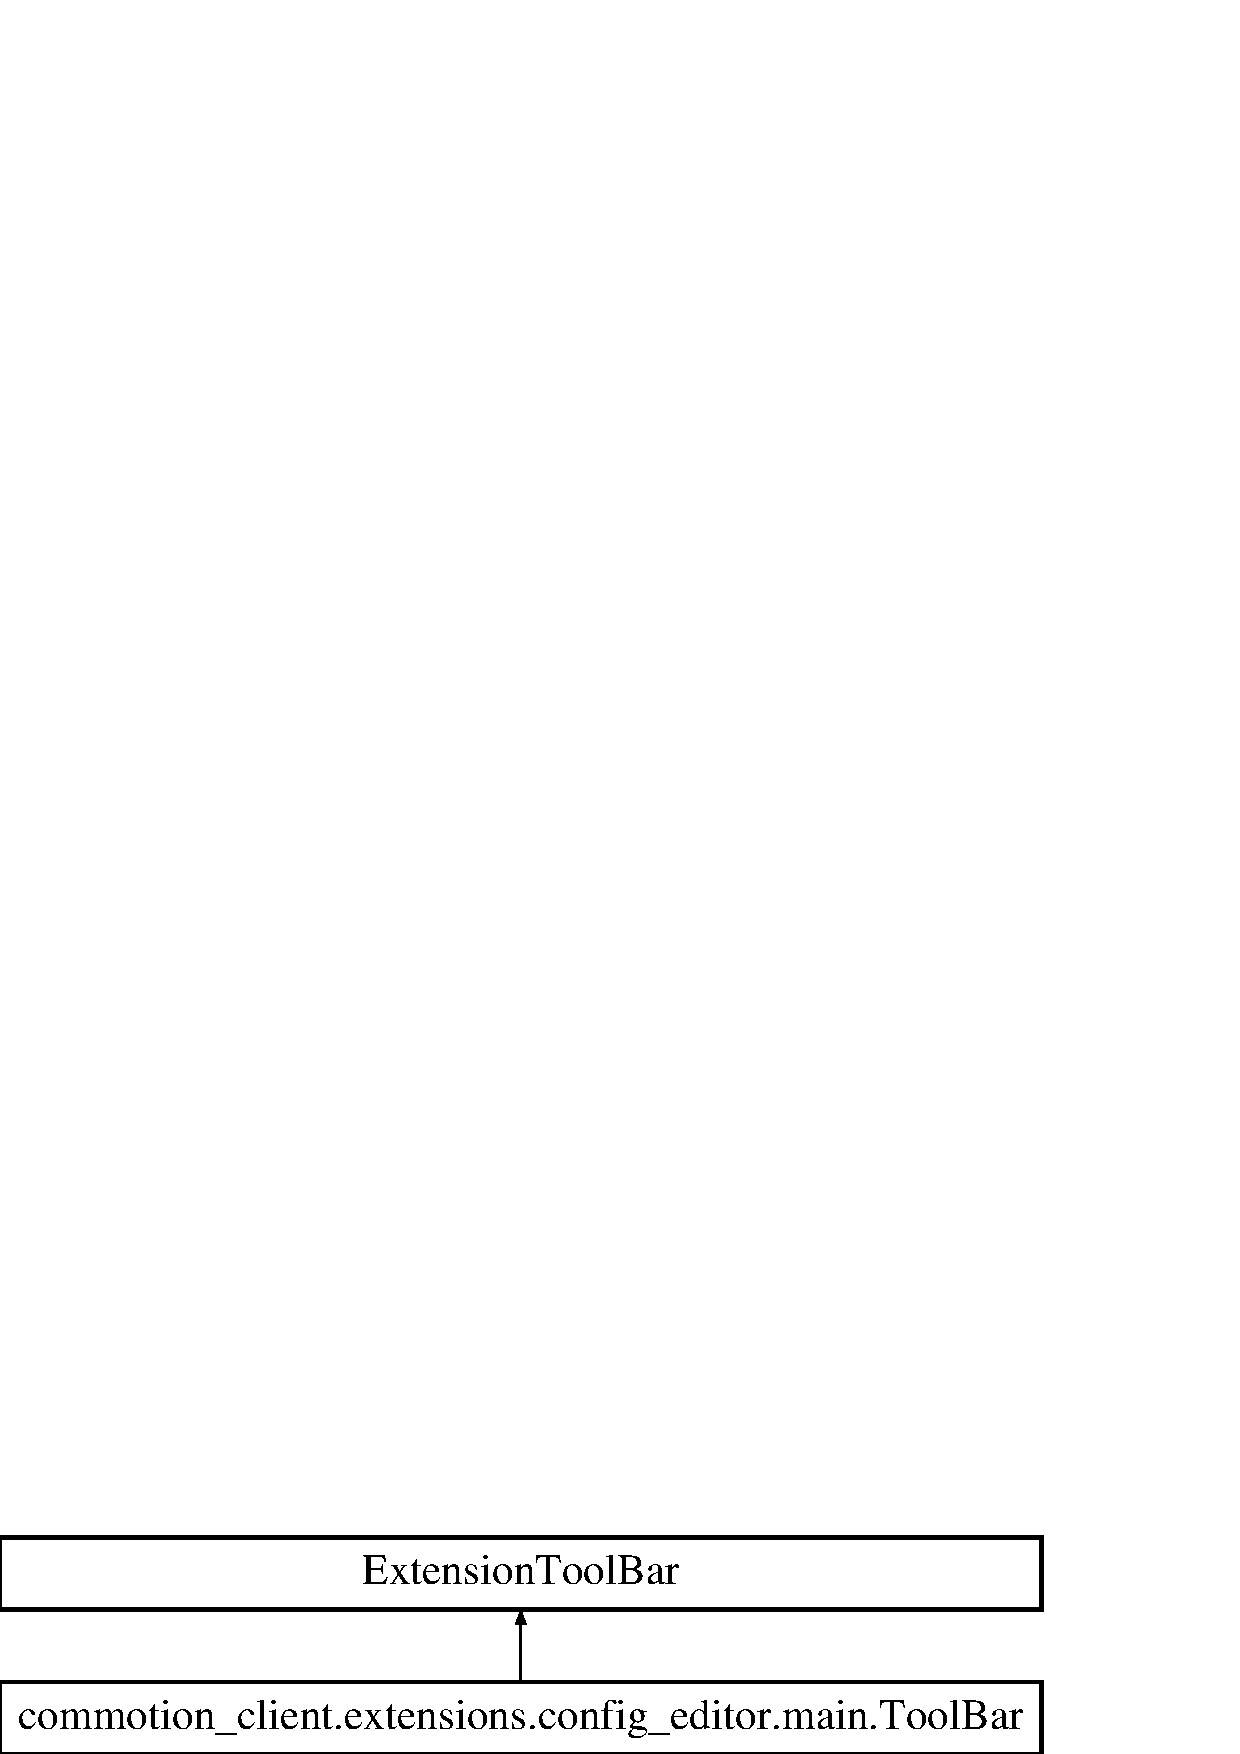
\includegraphics[height=2.000000cm]{classcommotion__client_1_1extensions_1_1config__editor_1_1main_1_1ToolBar}
\end{center}
\end{figure}


The documentation for this class was generated from the following file\+:\begin{DoxyCompactItemize}
\item 
commotion\+\_\+client/extensions/config\+\_\+editor/main.\+py\end{DoxyCompactItemize}

\hypertarget{classcommotion__client_1_1extensions_1_1unit__test__mock_1_1test__bar_1_1ToolBar}{\section{commotion\+\_\+client.\+extensions.\+unit\+\_\+test\+\_\+mock.\+test\+\_\+bar.\+Tool\+Bar Class Reference}
\label{classcommotion__client_1_1extensions_1_1unit__test__mock_1_1test__bar_1_1ToolBar}\index{commotion\+\_\+client.\+extensions.\+unit\+\_\+test\+\_\+mock.\+test\+\_\+bar.\+Tool\+Bar@{commotion\+\_\+client.\+extensions.\+unit\+\_\+test\+\_\+mock.\+test\+\_\+bar.\+Tool\+Bar}}
}
Inheritance diagram for commotion\+\_\+client.\+extensions.\+unit\+\_\+test\+\_\+mock.\+test\+\_\+bar.\+Tool\+Bar\+:\begin{figure}[H]
\begin{center}
\leavevmode
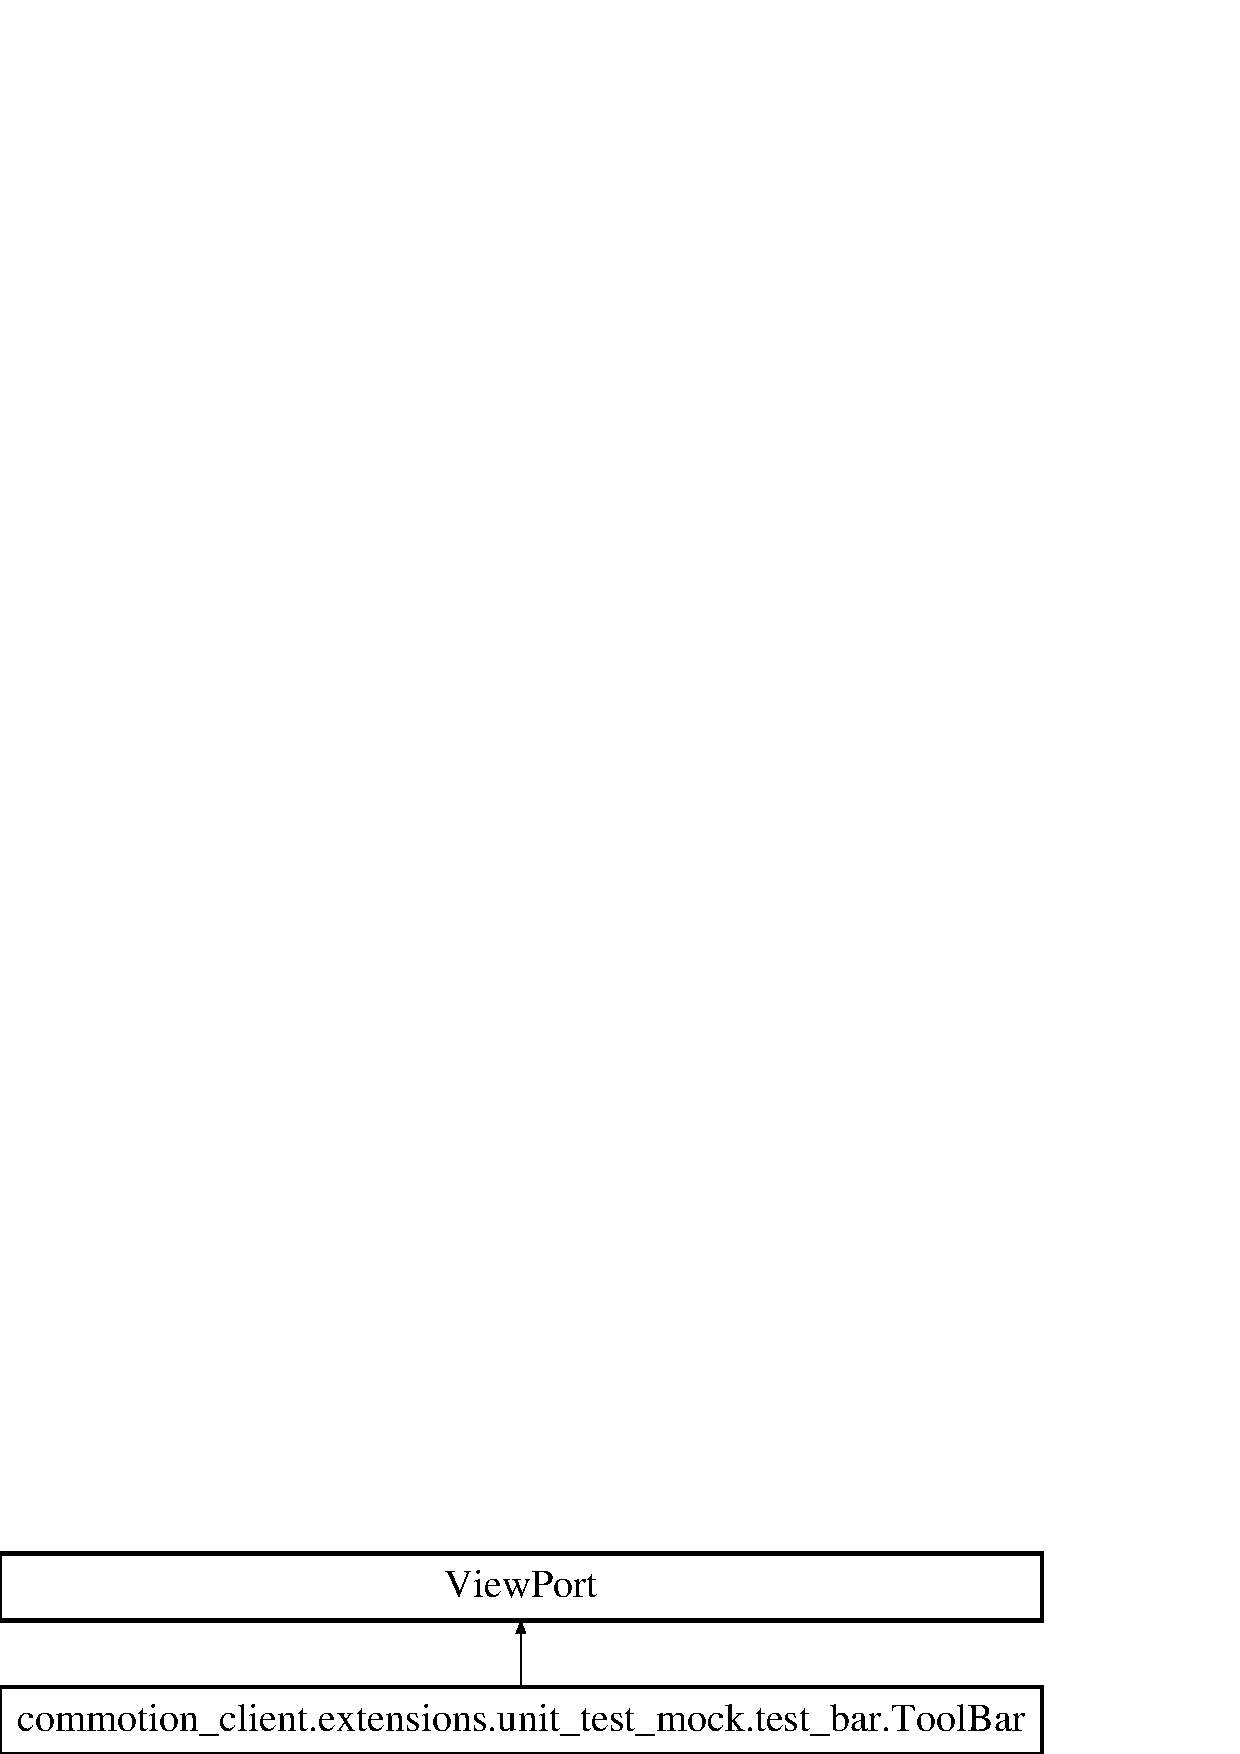
\includegraphics[height=2.000000cm]{classcommotion__client_1_1extensions_1_1unit__test__mock_1_1test__bar_1_1ToolBar}
\end{center}
\end{figure}
\subsection*{Public Member Functions}
\begin{DoxyCompactItemize}
\item 
\hypertarget{classcommotion__client_1_1extensions_1_1unit__test__mock_1_1test__bar_1_1ToolBar_a3b5b827110edea2c004ad18ac39c48c2}{def {\bfseries \+\_\+\+\_\+init\+\_\+\+\_\+}}\label{classcommotion__client_1_1extensions_1_1unit__test__mock_1_1test__bar_1_1ToolBar_a3b5b827110edea2c004ad18ac39c48c2}

\item 
\hypertarget{classcommotion__client_1_1extensions_1_1unit__test__mock_1_1test__bar_1_1ToolBar_a2590180f969a462b770cf5acadfdec89}{def {\bfseries send\+\_\+signal}}\label{classcommotion__client_1_1extensions_1_1unit__test__mock_1_1test__bar_1_1ToolBar_a2590180f969a462b770cf5acadfdec89}

\item 
def \hyperlink{classcommotion__client_1_1extensions_1_1unit__test__mock_1_1test__bar_1_1ToolBar_a88c0d36cbd949c0f9ded3423191b5af3}{send\+\_\+error}
\item 
\hypertarget{classcommotion__client_1_1extensions_1_1unit__test__mock_1_1test__bar_1_1ToolBar_a4c7d9655e04d923d46e5a8f4c230487d}{def {\bfseries is\+\_\+loaded}}\label{classcommotion__client_1_1extensions_1_1unit__test__mock_1_1test__bar_1_1ToolBar_a4c7d9655e04d923d46e5a8f4c230487d}

\end{DoxyCompactItemize}
\subsection*{Static Public Attributes}
\begin{DoxyCompactItemize}
\item 
\hypertarget{classcommotion__client_1_1extensions_1_1unit__test__mock_1_1test__bar_1_1ToolBar_aa5720861d390dece809a75b1877e7fd0}{tuple {\bfseries start\+\_\+report\+\_\+collection} = Qt\+Core.\+pyqt\+Signal()}\label{classcommotion__client_1_1extensions_1_1unit__test__mock_1_1test__bar_1_1ToolBar_aa5720861d390dece809a75b1877e7fd0}

\item 
\hypertarget{classcommotion__client_1_1extensions_1_1unit__test__mock_1_1test__bar_1_1ToolBar_a7254671f6fc142ecbdfc156ac33e3fc5}{tuple {\bfseries data\+\_\+report} = Qt\+Core.\+pyqt\+Signal(str, dict)}\label{classcommotion__client_1_1extensions_1_1unit__test__mock_1_1test__bar_1_1ToolBar_a7254671f6fc142ecbdfc156ac33e3fc5}

\item 
\hypertarget{classcommotion__client_1_1extensions_1_1unit__test__mock_1_1test__bar_1_1ToolBar_a5db11af55faa878867e2a1fd3d2bf164}{tuple {\bfseries error\+\_\+report} = Qt\+Core.\+pyqt\+Signal(str)}\label{classcommotion__client_1_1extensions_1_1unit__test__mock_1_1test__bar_1_1ToolBar_a5db11af55faa878867e2a1fd3d2bf164}

\end{DoxyCompactItemize}


\subsection{Detailed Description}
\begin{DoxyVerb}This is a mock extension and should not be used for ANYTHING user facing!
\end{DoxyVerb}
 

\subsection{Member Function Documentation}
\hypertarget{classcommotion__client_1_1extensions_1_1unit__test__mock_1_1test__bar_1_1ToolBar_a88c0d36cbd949c0f9ded3423191b5af3}{\index{commotion\+\_\+client\+::extensions\+::unit\+\_\+test\+\_\+mock\+::test\+\_\+bar\+::\+Tool\+Bar@{commotion\+\_\+client\+::extensions\+::unit\+\_\+test\+\_\+mock\+::test\+\_\+bar\+::\+Tool\+Bar}!send\+\_\+error@{send\+\_\+error}}
\index{send\+\_\+error@{send\+\_\+error}!commotion\+\_\+client\+::extensions\+::unit\+\_\+test\+\_\+mock\+::test\+\_\+bar\+::\+Tool\+Bar@{commotion\+\_\+client\+::extensions\+::unit\+\_\+test\+\_\+mock\+::test\+\_\+bar\+::\+Tool\+Bar}}
\subsubsection[{send\+\_\+error}]{\setlength{\rightskip}{0pt plus 5cm}def commotion\+\_\+client.\+extensions.\+unit\+\_\+test\+\_\+mock.\+test\+\_\+bar.\+Tool\+Bar.\+send\+\_\+error (
\begin{DoxyParamCaption}
\item[{}]{self}
\end{DoxyParamCaption}
)}}\label{classcommotion__client_1_1extensions_1_1unit__test__mock_1_1test__bar_1_1ToolBar_a88c0d36cbd949c0f9ded3423191b5af3}
\begin{DoxyVerb}HI\end{DoxyVerb}
 
\begin{DoxyCode}
37 
38     \textcolor{keyword}{def }\hyperlink{classcommotion__client_1_1extensions_1_1unit__test__mock_1_1test__bar_1_1ToolBar_a88c0d36cbd949c0f9ded3423191b5af3}{send\_error}(self):
39         \textcolor{stringliteral}{"""HI"""}
40         self.error\_report.emit(\textcolor{stringliteral}{"THIS IS AN ERROR MESSAGE!!!"})
41         \textcolor{keywordflow}{pass}

\end{DoxyCode}


The documentation for this class was generated from the following file\+:\begin{DoxyCompactItemize}
\item 
commotion\+\_\+client/extensions/unit\+\_\+test\+\_\+mock/test\+\_\+bar.\+py\end{DoxyCompactItemize}

\hypertarget{classcommotion__client_1_1GUI_1_1toolbar_1_1ToolBar}{\section{commotion\-\_\-client.\-G\-U\-I.\-toolbar.\-Tool\-Bar Class Reference}
\label{classcommotion__client_1_1GUI_1_1toolbar_1_1ToolBar}\index{commotion\-\_\-client.\-G\-U\-I.\-toolbar.\-Tool\-Bar@{commotion\-\_\-client.\-G\-U\-I.\-toolbar.\-Tool\-Bar}}
}
Inheritance diagram for commotion\-\_\-client.\-G\-U\-I.\-toolbar.\-Tool\-Bar\-:\begin{figure}[H]
\begin{center}
\leavevmode
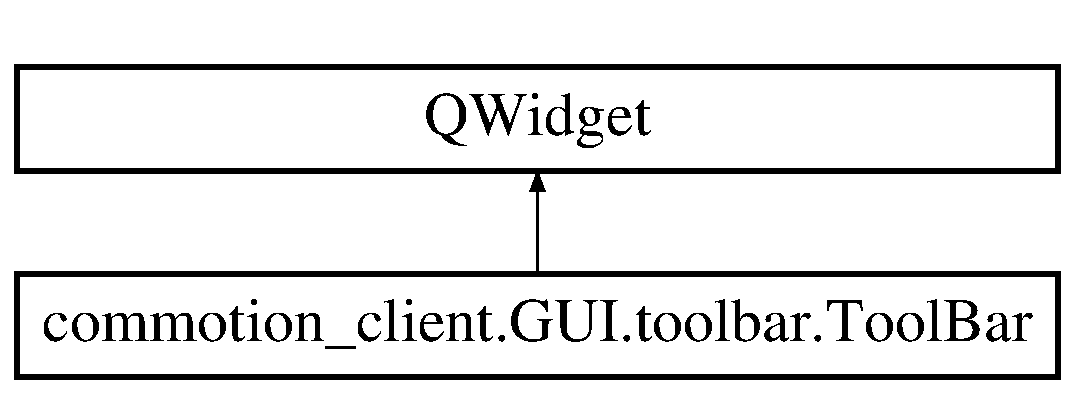
\includegraphics[height=2.000000cm]{classcommotion__client_1_1GUI_1_1toolbar_1_1ToolBar}
\end{center}
\end{figure}
\subsection*{Public Member Functions}
\begin{DoxyCompactItemize}
\item 
def \hyperlink{classcommotion__client_1_1GUI_1_1toolbar_1_1ToolBar_acea995f0bbf3a6e28c07b315e07b0af6}{\-\_\-\-\_\-init\-\_\-\-\_\-}
\item 
def \hyperlink{classcommotion__client_1_1GUI_1_1toolbar_1_1ToolBar_acb467ccaffdcd2c10fcce88a2d167079}{init\-\_\-settings}
\item 
def \hyperlink{classcommotion__client_1_1GUI_1_1toolbar_1_1ToolBar_a153dabe13871140e3d77226b986d8c37}{load\-\_\-settings}
\item 
def \hyperlink{classcommotion__client_1_1GUI_1_1toolbar_1_1ToolBar_a8fa89f6fa79c20123cdb74d3af3ecea5}{load\-\_\-about}
\item 
def \hyperlink{classcommotion__client_1_1GUI_1_1toolbar_1_1ToolBar_a186956c277f9ab85c6e1dcb73ec241ab}{load\-\_\-update}
\item 
def \hyperlink{classcommotion__client_1_1GUI_1_1toolbar_1_1ToolBar_a63bb48ec46de8e3982fb6e8ebcd05954}{load\-\_\-user}
\item 
def \hyperlink{classcommotion__client_1_1GUI_1_1toolbar_1_1ToolBar_ad0a0117438047cffdf421c9175c8e73a}{exit\-\_\-application}
\item 
def \hyperlink{classcommotion__client_1_1GUI_1_1toolbar_1_1ToolBar_a498f1b3352a8c1ee491921afb707fafa}{load\-\_\-extensions}
\item 
def \hyperlink{classcommotion__client_1_1GUI_1_1toolbar_1_1ToolBar_a232fde172cdeaf4c9c4b2dbc14a03cf3}{init\-\_\-user}
\item 
def \hyperlink{classcommotion__client_1_1GUI_1_1toolbar_1_1ToolBar_ad0e0bfc7e79a78a00253bebcc65c1a00}{init\-\_\-extension\-\_\-toolbar}
\end{DoxyCompactItemize}
\subsection*{Public Attributes}
\begin{DoxyCompactItemize}
\item 
\hypertarget{classcommotion__client_1_1GUI_1_1toolbar_1_1ToolBar_ac2987b2184e47fa5c08c1c753bafaa8b}{{\bfseries log}}\label{classcommotion__client_1_1GUI_1_1toolbar_1_1ToolBar_ac2987b2184e47fa5c08c1c753bafaa8b}

\item 
\hypertarget{classcommotion__client_1_1GUI_1_1toolbar_1_1ToolBar_a5ec3c619935f7e0626f9cb608be8e27f}{{\bfseries translate}}\label{classcommotion__client_1_1GUI_1_1toolbar_1_1ToolBar_a5ec3c619935f7e0626f9cb608be8e27f}

\item 
\hypertarget{classcommotion__client_1_1GUI_1_1toolbar_1_1ToolBar_a34d12135499302eef49fbe526cd0d66b}{{\bfseries viewport}}\label{classcommotion__client_1_1GUI_1_1toolbar_1_1ToolBar_a34d12135499302eef49fbe526cd0d66b}

\item 
\hypertarget{classcommotion__client_1_1GUI_1_1toolbar_1_1ToolBar_a30d7fa9d80355eb4d3d214cc0511de88}{{\bfseries toolbar}}\label{classcommotion__client_1_1GUI_1_1toolbar_1_1ToolBar_a30d7fa9d80355eb4d3d214cc0511de88}

\item 
\hypertarget{classcommotion__client_1_1GUI_1_1toolbar_1_1ToolBar_af5761f237999d6146ebe2e296306e5b7}{{\bfseries settings}}\label{classcommotion__client_1_1GUI_1_1toolbar_1_1ToolBar_af5761f237999d6146ebe2e296306e5b7}

\end{DoxyCompactItemize}


\subsection{Detailed Description}
\begin{DoxyVerb}The Core toolbar object that populates manditory toolbar sections.
\end{DoxyVerb}
 

\subsection{Constructor \& Destructor Documentation}
\hypertarget{classcommotion__client_1_1GUI_1_1toolbar_1_1ToolBar_acea995f0bbf3a6e28c07b315e07b0af6}{\index{commotion\-\_\-client\-::\-G\-U\-I\-::toolbar\-::\-Tool\-Bar@{commotion\-\_\-client\-::\-G\-U\-I\-::toolbar\-::\-Tool\-Bar}!\-\_\-\-\_\-init\-\_\-\-\_\-@{\-\_\-\-\_\-init\-\_\-\-\_\-}}
\index{\-\_\-\-\_\-init\-\_\-\-\_\-@{\-\_\-\-\_\-init\-\_\-\-\_\-}!commotion_client::GUI::toolbar::ToolBar@{commotion\-\_\-client\-::\-G\-U\-I\-::toolbar\-::\-Tool\-Bar}}
\subsubsection[{\-\_\-\-\_\-init\-\_\-\-\_\-}]{\setlength{\rightskip}{0pt plus 5cm}def commotion\-\_\-client.\-G\-U\-I.\-toolbar.\-Tool\-Bar.\-\_\-\-\_\-init\-\_\-\-\_\- (
\begin{DoxyParamCaption}
\item[{}]{self, }
\item[{}]{parent = {\ttfamily None}, }
\item[{}]{extension\-\_\-toolbar = {\ttfamily None}, }
\item[{}]{viewport}
\end{DoxyParamCaption}
)}}\label{classcommotion__client_1_1GUI_1_1toolbar_1_1ToolBar_acea995f0bbf3a6e28c07b315e07b0af6}
\begin{DoxyVerb}Creates the core toolbar including any extension toolbar passed to it.

Initializes the core functionality of the toolbar. If an extension_toolbar object is also passed to the toolbar it will attempt to add the extension toolbar into itself.

Args:
  extension_toolbar (object): The extension specific menu-item to be used by an extension. This class is derived from the "commotion_client/GUI/extension_toolbar.ExtensionToolBar" object.
  viewport (object): The current viewport. This allows menu_items to have its actions interact with the current viewport.

Raises:
  exception: Description.\end{DoxyVerb}
 

References commotion\-\_\-client.\-G\-U\-I.\-main\-\_\-window.\-Main\-Window.\-\_\-dirty, commotion\-\_\-client.\-G\-U\-I.\-extension\-\_\-toolbar.\-Extension\-Tool\-Bar.\-\_\-dirty, commotion\-\_\-client.\-G\-U\-I.\-toolbar.\-Tool\-Bar.\-\_\-dirty, commotion\-\_\-client.\-extensions.\-config\-\_\-editor.\-main.\-View\-Port.\-\_\-dirty, commotion\-\_\-client.\-G\-U\-I.\-extension\-\_\-toolbar.\-Menu\-Item.\-\_\-dirty, commotion\-\_\-client.\-G\-U\-I.\-toolbar.\-Tool\-Bar.\-init\-\_\-settings(), commotion\-\_\-client.\-G\-U\-I.\-system\-\_\-tray.\-Tray\-Icon.\-log, commotion\-\_\-client.\-G\-U\-I.\-menu\-\_\-bar.\-Menu\-Bar.\-log, commotion\-\_\-client.\-G\-U\-I.\-crash\-\_\-report.\-Crash\-Report.\-log, commotion\-\_\-client.\-extensions.\-config\-\_\-editor.\-main.\-View\-Port.\-log, commotion\-\_\-client.\-G\-U\-I.\-main\-\_\-window.\-Main\-Window.\-log, commotion\-\_\-client.\-G\-U\-I.\-toolbar.\-Tool\-Bar.\-log, commotion\-\_\-client.\-G\-U\-I.\-extension\-\_\-toolbar.\-Extension\-Tool\-Bar.\-log, commotion\-\_\-client.\-commotion\-\_\-client.\-Hold\-State\-During\-Restart.\-log, commotion\-\_\-client.\-G\-U\-I.\-extension\-\_\-toolbar.\-Menu\-Item.\-log, commotion\-\_\-client.\-G\-U\-I.\-crash\-\_\-report.\-Report\-Gatherer.\-log, commotion\-\_\-client.\-commotion\-\_\-client.\-Commotion\-Client\-Application.\-log, commotion\-\_\-client.\-G\-U\-I.\-toolbar.\-Tool\-Bar.\-settings, commotion\-\_\-client.\-G\-U\-I.\-toolbar.\-Tool\-Bar.\-toolbar, commotion\-\_\-client.\-G\-U\-I.\-main\-\_\-window.\-Main\-Window.\-toolbar, commotion\-\_\-client.\-G\-U\-I.\-menu\-\_\-bar.\-Menu\-Bar.\-translate, commotion\-\_\-client.\-extensions.\-config\-\_\-editor.\-main.\-View\-Port.\-translate, commotion\-\_\-client.\-G\-U\-I.\-main\-\_\-window.\-Main\-Window.\-translate, commotion\-\_\-client.\-G\-U\-I.\-extension\-\_\-toolbar.\-Extension\-Tool\-Bar.\-translate, commotion\-\_\-client.\-G\-U\-I.\-toolbar.\-Tool\-Bar.\-translate, commotion\-\_\-client.\-G\-U\-I.\-extension\-\_\-toolbar.\-Menu\-Item.\-translate, commotion\-\_\-client.\-commotion\-\_\-client.\-Commotion\-Client\-Application.\-translate, commotion\-\_\-client.\-G\-U\-I.\-extension\-\_\-toolbar.\-Extension\-Tool\-Bar.\-viewport, commotion\-\_\-client.\-G\-U\-I.\-toolbar.\-Tool\-Bar.\-viewport, commotion\-\_\-client.\-G\-U\-I.\-main\-\_\-window.\-Main\-Window.\-viewport, and commotion\-\_\-client.\-G\-U\-I.\-extension\-\_\-toolbar.\-Menu\-Item.\-viewport.


\begin{DoxyCode}
30 
31     \textcolor{keyword}{def }\hyperlink{classcommotion__client_1_1GUI_1_1toolbar_1_1ToolBar_acea995f0bbf3a6e28c07b315e07b0af6}{\_\_init\_\_}(self, parent=None, extension\_toolbar=None, viewport):
32         \textcolor{stringliteral}{"""Creates the core toolbar including any extension toolbar passed to it.}
33 \textcolor{stringliteral}{        }
34 \textcolor{stringliteral}{        Initializes the core functionality of the toolbar. If an extension\_toolbar object is also passed to
       the toolbar it will attempt to add the extension toolbar into itself.}
35 \textcolor{stringliteral}{        }
36 \textcolor{stringliteral}{        Args:}
37 \textcolor{stringliteral}{          extension\_toolbar (object): The extension specific menu-item to be used by an extension. This
       class is derived from the "commotion\_client/GUI/extension\_toolbar.ExtensionToolBar" object.}
38 \textcolor{stringliteral}{          viewport (object): The current viewport. This allows menu\_items to have its actions interact with
       the current viewport.}
39 \textcolor{stringliteral}{}
40 \textcolor{stringliteral}{        Raises:}
41 \textcolor{stringliteral}{          exception: Description.}
42 \textcolor{stringliteral}{        }
43 \textcolor{stringliteral}{        """}
44         super().\hyperlink{classcommotion__client_1_1GUI_1_1toolbar_1_1ToolBar_acea995f0bbf3a6e28c07b315e07b0af6}{\_\_init\_\_}()
45         self.\hyperlink{classcommotion__client_1_1GUI_1_1toolbar_1_1ToolBar_a3d4267f273f2262c1b97b9ed3e04aebd}{\_dirty} = \textcolor{keyword}{False}
46         self.\hyperlink{classcommotion__client_1_1GUI_1_1toolbar_1_1ToolBar_ac2987b2184e47fa5c08c1c753bafaa8b}{log} = logging.getLogger(\textcolor{stringliteral}{"commotion\_client."}+\_\_name\_\_)
47         self.\hyperlink{classcommotion__client_1_1GUI_1_1toolbar_1_1ToolBar_a5ec3c619935f7e0626f9cb608be8e27f}{translate} = QtCore.QCoreApplication.translate
48 
49         self.\hyperlink{classcommotion__client_1_1GUI_1_1toolbar_1_1ToolBar_a34d12135499302eef49fbe526cd0d66b}{viewport} = viewport
50         \textcolor{comment}{#Create toolbar object}
51         self.\hyperlink{classcommotion__client_1_1GUI_1_1toolbar_1_1ToolBar_a30d7fa9d80355eb4d3d214cc0511de88}{toolbar} = QtGui.QToolBar(self)
52         \textcolor{comment}{#Create & add settings item}
53         self.\hyperlink{classcommotion__client_1_1GUI_1_1toolbar_1_1ToolBar_af5761f237999d6146ebe2e296306e5b7}{settings} = self.\hyperlink{classcommotion__client_1_1GUI_1_1toolbar_1_1ToolBar_acb467ccaffdcd2c10fcce88a2d167079}{init\_settings}()
54         self.toolbar.addWidget(self.\hyperlink{classcommotion__client_1_1GUI_1_1toolbar_1_1ToolBar_af5761f237999d6146ebe2e296306e5b7}{settings})
55         \textcolor{comment}{#Create & add user item}
56 \textcolor{comment}{#        self.user = self.init\_user()}
57 \textcolor{comment}{#        self.toolbar.addWidget(self.user)}
58         \textcolor{comment}{#Create extension toolbar section if needed}
59 \textcolor{comment}{#        if extension\_toolbar:}
60 \textcolor{comment}{#            self.extension\_toolbar = extension\_toolbar(self, viewport)}
61 \textcolor{comment}{#            self.init\_extension\_toolbar()}

\end{DoxyCode}


\subsection{Member Function Documentation}
\hypertarget{classcommotion__client_1_1GUI_1_1toolbar_1_1ToolBar_ad0a0117438047cffdf421c9175c8e73a}{\index{commotion\-\_\-client\-::\-G\-U\-I\-::toolbar\-::\-Tool\-Bar@{commotion\-\_\-client\-::\-G\-U\-I\-::toolbar\-::\-Tool\-Bar}!exit\-\_\-application@{exit\-\_\-application}}
\index{exit\-\_\-application@{exit\-\_\-application}!commotion_client::GUI::toolbar::ToolBar@{commotion\-\_\-client\-::\-G\-U\-I\-::toolbar\-::\-Tool\-Bar}}
\subsubsection[{exit\-\_\-application}]{\setlength{\rightskip}{0pt plus 5cm}def commotion\-\_\-client.\-G\-U\-I.\-toolbar.\-Tool\-Bar.\-exit\-\_\-application (
\begin{DoxyParamCaption}
\item[{}]{self}
\end{DoxyParamCaption}
)}}\label{classcommotion__client_1_1GUI_1_1toolbar_1_1ToolBar_ad0a0117438047cffdf421c9175c8e73a}
\begin{DoxyVerb}Exits the application.\end{DoxyVerb}
 

Referenced by commotion\-\_\-client.\-G\-U\-I.\-toolbar.\-Tool\-Bar.\-init\-\_\-settings(), and commotion\-\_\-client.\-G\-U\-I.\-toolbar\-\_\-builder.\-Tool\-Bar.\-init\-\_\-settings().


\begin{DoxyCode}
124 
125     \textcolor{keyword}{def }\hyperlink{classcommotion__client_1_1GUI_1_1toolbar_1_1ToolBar_ad0a0117438047cffdf421c9175c8e73a}{exit\_application}(self):
126        \textcolor{stringliteral}{"""Exits the application."""}
127        \textcolor{keywordflow}{pass}
       
\end{DoxyCode}
\hypertarget{classcommotion__client_1_1GUI_1_1toolbar_1_1ToolBar_ad0e0bfc7e79a78a00253bebcc65c1a00}{\index{commotion\-\_\-client\-::\-G\-U\-I\-::toolbar\-::\-Tool\-Bar@{commotion\-\_\-client\-::\-G\-U\-I\-::toolbar\-::\-Tool\-Bar}!init\-\_\-extension\-\_\-toolbar@{init\-\_\-extension\-\_\-toolbar}}
\index{init\-\_\-extension\-\_\-toolbar@{init\-\_\-extension\-\_\-toolbar}!commotion_client::GUI::toolbar::ToolBar@{commotion\-\_\-client\-::\-G\-U\-I\-::toolbar\-::\-Tool\-Bar}}
\subsubsection[{init\-\_\-extension\-\_\-toolbar}]{\setlength{\rightskip}{0pt plus 5cm}def commotion\-\_\-client.\-G\-U\-I.\-toolbar.\-Tool\-Bar.\-init\-\_\-extension\-\_\-toolbar (
\begin{DoxyParamCaption}
\item[{}]{self}
\end{DoxyParamCaption}
)}}\label{classcommotion__client_1_1GUI_1_1toolbar_1_1ToolBar_ad0e0bfc7e79a78a00253bebcc65c1a00}
\begin{DoxyVerb}short description

long description

Args:
name (type): Description.

Returns:
Description.

Raises:
exception: Description.\end{DoxyVerb}
 
\begin{DoxyCode}
151 
152     \textcolor{keyword}{def }\hyperlink{classcommotion__client_1_1GUI_1_1toolbar_1_1ToolBar_ad0e0bfc7e79a78a00253bebcc65c1a00}{init\_extension\_toolbar}(self):
153         \textcolor{stringliteral}{"""short description}
154 \textcolor{stringliteral}{        }
155 \textcolor{stringliteral}{        long description}
156 \textcolor{stringliteral}{        }
157 \textcolor{stringliteral}{        Args:}
158 \textcolor{stringliteral}{        name (type): Description.}
159 \textcolor{stringliteral}{        }
160 \textcolor{stringliteral}{        Returns:}
161 \textcolor{stringliteral}{        Description.}
162 \textcolor{stringliteral}{        }
163 \textcolor{stringliteral}{        Raises:}
164 \textcolor{stringliteral}{        exception: Description.}
165 \textcolor{stringliteral}{        }
166 \textcolor{stringliteral}{        """}
167         \textcolor{keywordflow}{for} menu\_item \textcolor{keywordflow}{in} self.extension\_menu.menu\_items:
168             \textcolor{keywordflow}{try}:
169                 self.toolbar.addWidget(menu\_item)
\end{DoxyCode}
\hypertarget{classcommotion__client_1_1GUI_1_1toolbar_1_1ToolBar_acb467ccaffdcd2c10fcce88a2d167079}{\index{commotion\-\_\-client\-::\-G\-U\-I\-::toolbar\-::\-Tool\-Bar@{commotion\-\_\-client\-::\-G\-U\-I\-::toolbar\-::\-Tool\-Bar}!init\-\_\-settings@{init\-\_\-settings}}
\index{init\-\_\-settings@{init\-\_\-settings}!commotion_client::GUI::toolbar::ToolBar@{commotion\-\_\-client\-::\-G\-U\-I\-::toolbar\-::\-Tool\-Bar}}
\subsubsection[{init\-\_\-settings}]{\setlength{\rightskip}{0pt plus 5cm}def commotion\-\_\-client.\-G\-U\-I.\-toolbar.\-Tool\-Bar.\-init\-\_\-settings (
\begin{DoxyParamCaption}
\item[{}]{self}
\end{DoxyParamCaption}
)}}\label{classcommotion__client_1_1GUI_1_1toolbar_1_1ToolBar_acb467ccaffdcd2c10fcce88a2d167079}
\begin{DoxyVerb}short description

long description

Args:
name (type): Description.

Returns:
Description.

Raises:
exception: Description.\end{DoxyVerb}
 

References commotion\-\_\-client.\-G\-U\-I.\-toolbar.\-Tool\-Bar.\-exit\-\_\-application(), commotion\-\_\-client.\-G\-U\-I.\-toolbar.\-Tool\-Bar.\-load\-\_\-about(), commotion\-\_\-client.\-G\-U\-I.\-toolbar.\-Tool\-Bar.\-load\-\_\-extensions(), commotion\-\_\-client.\-G\-U\-I.\-toolbar.\-Tool\-Bar.\-load\-\_\-settings(), commotion\-\_\-client.\-G\-U\-I.\-main\-\_\-window.\-Main\-Window.\-load\-\_\-settings(), commotion\-\_\-client.\-G\-U\-I.\-toolbar.\-Tool\-Bar.\-load\-\_\-update(), commotion\-\_\-client.\-G\-U\-I.\-menu\-\_\-bar.\-Menu\-Bar.\-translate, commotion\-\_\-client.\-extensions.\-config\-\_\-editor.\-main.\-View\-Port.\-translate, commotion\-\_\-client.\-G\-U\-I.\-main\-\_\-window.\-Main\-Window.\-translate, commotion\-\_\-client.\-G\-U\-I.\-toolbar.\-Tool\-Bar.\-translate, commotion\-\_\-client.\-G\-U\-I.\-extension\-\_\-toolbar.\-Extension\-Tool\-Bar.\-translate, commotion\-\_\-client.\-G\-U\-I.\-extension\-\_\-toolbar.\-Menu\-Item.\-translate, commotion\-\_\-client.\-commotion\-\_\-client.\-Commotion\-Client\-Application.\-translate, commotion\-\_\-client.\-G\-U\-I.\-extension\-\_\-toolbar.\-Extension\-Tool\-Bar.\-viewport, commotion\-\_\-client.\-G\-U\-I.\-toolbar.\-Tool\-Bar.\-viewport, commotion\-\_\-client.\-G\-U\-I.\-main\-\_\-window.\-Main\-Window.\-viewport, and commotion\-\_\-client.\-G\-U\-I.\-extension\-\_\-toolbar.\-Menu\-Item.\-viewport.



Referenced by commotion\-\_\-client.\-G\-U\-I.\-toolbar\-\_\-builder.\-Tool\-Bar.\-\_\-\-\_\-init\-\_\-\-\_\-(), and commotion\-\_\-client.\-G\-U\-I.\-toolbar.\-Tool\-Bar.\-\_\-\-\_\-init\-\_\-\-\_\-().


\begin{DoxyCode}
62 
63     \textcolor{keyword}{def }\hyperlink{classcommotion__client_1_1GUI_1_1toolbar_1_1ToolBar_acb467ccaffdcd2c10fcce88a2d167079}{init\_settings}(self):
64         \textcolor{stringliteral}{"""short description}
65 \textcolor{stringliteral}{        }
66 \textcolor{stringliteral}{        long description}
67 \textcolor{stringliteral}{        }
68 \textcolor{stringliteral}{        Args:}
69 \textcolor{stringliteral}{        name (type): Description.}
70 \textcolor{stringliteral}{        }
71 \textcolor{stringliteral}{        Returns:}
72 \textcolor{stringliteral}{        Description.}
73 \textcolor{stringliteral}{        }
74 \textcolor{stringliteral}{        Raises:}
75 \textcolor{stringliteral}{        exception: Description.}
76 \textcolor{stringliteral}{        }
77 \textcolor{stringliteral}{        """}
78         settings\_menu = \hyperlink{classcommotion__client_1_1GUI_1_1extension__toolbar_1_1MenuItem}{extension\_toolbar.MenuItem}(self, self.
      \hyperlink{classcommotion__client_1_1GUI_1_1toolbar_1_1ToolBar_a34d12135499302eef49fbe526cd0d66b}{viewport})
79         settings\_menu.setIcon(extension\_toolbar.icon.settings)
80         settings\_menu.setText(self.\hyperlink{classcommotion__client_1_1GUI_1_1toolbar_1_1ToolBar_a5ec3c619935f7e0626f9cb608be8e27f}{translate}(\textcolor{stringliteral}{"menu"}, \textcolor{stringliteral}{"Settings"}))
81         settings\_menu.set\_menu = \textcolor{keyword}{True}
82         extensions\_item = QtGui.QAction(self.\hyperlink{classcommotion__client_1_1GUI_1_1toolbar_1_1ToolBar_a5ec3c619935f7e0626f9cb608be8e27f}{translate}(\textcolor{stringliteral}{"menu"}, \textcolor{stringliteral}{"&Extensions"}),
83                                         statusTip=self.\hyperlink{classcommotion__client_1_1GUI_1_1toolbar_1_1ToolBar_a5ec3c619935f7e0626f9cb608be8e27f}{translate}(\textcolor{stringliteral}{"menu"}, \textcolor{stringliteral}{"Open the extensions
       menu."}),
84                                         triggered=self.\hyperlink{classcommotion__client_1_1GUI_1_1toolbar_1_1ToolBar_a498f1b3352a8c1ee491921afb707fafa}{load\_extensions},
85                                         parent=settings\_menu)
86         
87         settings\_item = QtGui.QAction(self.\hyperlink{classcommotion__client_1_1GUI_1_1toolbar_1_1ToolBar_a5ec3c619935f7e0626f9cb608be8e27f}{translate}(\textcolor{stringliteral}{"menu"}, \textcolor{stringliteral}{"&Settings"}),
88                                       QtGui.QIcon(\textcolor{stringliteral}{"icons/load.png"}),
89                                       statusTip=self.\hyperlink{classcommotion__client_1_1GUI_1_1toolbar_1_1ToolBar_a5ec3c619935f7e0626f9cb608be8e27f}{translate}(\textcolor{stringliteral}{"menu"}, \textcolor{stringliteral}{"Open the settings menu."}),
90                                       triggered=self.\hyperlink{classcommotion__client_1_1GUI_1_1toolbar_1_1ToolBar_a153dabe13871140e3d77226b986d8c37}{load\_settings},
91                                       parent=settings\_menu)
92         about\_item = QtGui.QAction(self.\hyperlink{classcommotion__client_1_1GUI_1_1toolbar_1_1ToolBar_a5ec3c619935f7e0626f9cb608be8e27f}{translate}(\textcolor{stringliteral}{"menu"}, \textcolor{stringliteral}{"&About"}),
93                                    QtGui.QIcon(\textcolor{stringliteral}{"icons/load.png"}),
94                                    statusTip=self.\hyperlink{classcommotion__client_1_1GUI_1_1toolbar_1_1ToolBar_a5ec3c619935f7e0626f9cb608be8e27f}{translate}(\textcolor{stringliteral}{"menu"}, \textcolor{stringliteral}{"Open the \(\backslash\)'about us\(\backslash\)' page"}),
95                                    triggered=self.\hyperlink{classcommotion__client_1_1GUI_1_1toolbar_1_1ToolBar_a8fa89f6fa79c20123cdb74d3af3ecea5}{load\_about},
96                                    parent=settings\_menu)
97         exit\_item = QtGui.QAction(self.\hyperlink{classcommotion__client_1_1GUI_1_1toolbar_1_1ToolBar_a5ec3c619935f7e0626f9cb608be8e27f}{translate}(\textcolor{stringliteral}{"menu"}, \textcolor{stringliteral}{"&Exit"}),
98                                   QtGui.QIcon(\textcolor{stringliteral}{"icons/load.png"}),
99                                   statusTip=self.\hyperlink{classcommotion__client_1_1GUI_1_1toolbar_1_1ToolBar_a5ec3c619935f7e0626f9cb608be8e27f}{translate}(\textcolor{stringliteral}{"menu"}, \textcolor{stringliteral}{"Exit the application."}),
100                                   triggered=self.\hyperlink{classcommotion__client_1_1GUI_1_1toolbar_1_1ToolBar_ad0a0117438047cffdf421c9175c8e73a}{exit\_application},
101                                   parent=settings\_menu)
102         update\_item = QtGui.QAction(self.\hyperlink{classcommotion__client_1_1GUI_1_1toolbar_1_1ToolBar_a5ec3c619935f7e0626f9cb608be8e27f}{translate}(\textcolor{stringliteral}{"menu"}, \textcolor{stringliteral}{"&Update"}),
103                                     QtGui.QIcon(\textcolor{stringliteral}{"icons/load.png"}),
104                                     statusTip=self.\hyperlink{classcommotion__client_1_1GUI_1_1toolbar_1_1ToolBar_a5ec3c619935f7e0626f9cb608be8e27f}{translate}(\textcolor{stringliteral}{"menu"}, \textcolor{stringliteral}{"Open the updates page."}),
105                                     triggered=self.\hyperlink{classcommotion__client_1_1GUI_1_1toolbar_1_1ToolBar_a186956c277f9ab85c6e1dcb73ec241ab}{load\_update},
106                                     parent=settings\_menu)
107         \textcolor{keywordflow}{return} settings\_menu
        
\end{DoxyCode}
\hypertarget{classcommotion__client_1_1GUI_1_1toolbar_1_1ToolBar_a232fde172cdeaf4c9c4b2dbc14a03cf3}{\index{commotion\-\_\-client\-::\-G\-U\-I\-::toolbar\-::\-Tool\-Bar@{commotion\-\_\-client\-::\-G\-U\-I\-::toolbar\-::\-Tool\-Bar}!init\-\_\-user@{init\-\_\-user}}
\index{init\-\_\-user@{init\-\_\-user}!commotion_client::GUI::toolbar::ToolBar@{commotion\-\_\-client\-::\-G\-U\-I\-::toolbar\-::\-Tool\-Bar}}
\subsubsection[{init\-\_\-user}]{\setlength{\rightskip}{0pt plus 5cm}def commotion\-\_\-client.\-G\-U\-I.\-toolbar.\-Tool\-Bar.\-init\-\_\-user (
\begin{DoxyParamCaption}
\item[{}]{self}
\end{DoxyParamCaption}
)}}\label{classcommotion__client_1_1GUI_1_1toolbar_1_1ToolBar_a232fde172cdeaf4c9c4b2dbc14a03cf3}
\begin{DoxyVerb}short description

long description

Args:
name (type): Description.

Returns:
Description.

Raises:
exception: Description.\end{DoxyVerb}
 
\begin{DoxyCode}
132 
133     \textcolor{keyword}{def }\hyperlink{classcommotion__client_1_1GUI_1_1toolbar_1_1ToolBar_a232fde172cdeaf4c9c4b2dbc14a03cf3}{init\_user}(self):
134         \textcolor{stringliteral}{"""short description}
135 \textcolor{stringliteral}{        }
136 \textcolor{stringliteral}{        long description}
137 \textcolor{stringliteral}{        }
138 \textcolor{stringliteral}{        Args:}
139 \textcolor{stringliteral}{        name (type): Description.}
140 \textcolor{stringliteral}{        }
141 \textcolor{stringliteral}{        Returns:}
142 \textcolor{stringliteral}{        Description.}
143 \textcolor{stringliteral}{        }
144 \textcolor{stringliteral}{        Raises:}
145 \textcolor{stringliteral}{        exception: Description.}
146 \textcolor{stringliteral}{        }
147 \textcolor{stringliteral}{        """}
148         \textcolor{keywordflow}{pass}
149 
150 

\end{DoxyCode}
\hypertarget{classcommotion__client_1_1GUI_1_1toolbar_1_1ToolBar_a8fa89f6fa79c20123cdb74d3af3ecea5}{\index{commotion\-\_\-client\-::\-G\-U\-I\-::toolbar\-::\-Tool\-Bar@{commotion\-\_\-client\-::\-G\-U\-I\-::toolbar\-::\-Tool\-Bar}!load\-\_\-about@{load\-\_\-about}}
\index{load\-\_\-about@{load\-\_\-about}!commotion_client::GUI::toolbar::ToolBar@{commotion\-\_\-client\-::\-G\-U\-I\-::toolbar\-::\-Tool\-Bar}}
\subsubsection[{load\-\_\-about}]{\setlength{\rightskip}{0pt plus 5cm}def commotion\-\_\-client.\-G\-U\-I.\-toolbar.\-Tool\-Bar.\-load\-\_\-about (
\begin{DoxyParamCaption}
\item[{}]{self}
\end{DoxyParamCaption}
)}}\label{classcommotion__client_1_1GUI_1_1toolbar_1_1ToolBar_a8fa89f6fa79c20123cdb74d3af3ecea5}
\begin{DoxyVerb}Opens the about page in the main viewport \end{DoxyVerb}
 

Referenced by commotion\-\_\-client.\-G\-U\-I.\-toolbar.\-Tool\-Bar.\-init\-\_\-settings(), and commotion\-\_\-client.\-G\-U\-I.\-toolbar\-\_\-builder.\-Tool\-Bar.\-init\-\_\-settings().


\begin{DoxyCode}
112 
113     \textcolor{keyword}{def }\hyperlink{classcommotion__client_1_1GUI_1_1toolbar_1_1ToolBar_a8fa89f6fa79c20123cdb74d3af3ecea5}{load\_about}(self):
114        \textcolor{stringliteral}{"""Opens the about page in the main viewport """}
115        \textcolor{keywordflow}{pass}
       
\end{DoxyCode}
\hypertarget{classcommotion__client_1_1GUI_1_1toolbar_1_1ToolBar_a498f1b3352a8c1ee491921afb707fafa}{\index{commotion\-\_\-client\-::\-G\-U\-I\-::toolbar\-::\-Tool\-Bar@{commotion\-\_\-client\-::\-G\-U\-I\-::toolbar\-::\-Tool\-Bar}!load\-\_\-extensions@{load\-\_\-extensions}}
\index{load\-\_\-extensions@{load\-\_\-extensions}!commotion_client::GUI::toolbar::ToolBar@{commotion\-\_\-client\-::\-G\-U\-I\-::toolbar\-::\-Tool\-Bar}}
\subsubsection[{load\-\_\-extensions}]{\setlength{\rightskip}{0pt plus 5cm}def commotion\-\_\-client.\-G\-U\-I.\-toolbar.\-Tool\-Bar.\-load\-\_\-extensions (
\begin{DoxyParamCaption}
\item[{}]{self}
\end{DoxyParamCaption}
)}}\label{classcommotion__client_1_1GUI_1_1toolbar_1_1ToolBar_a498f1b3352a8c1ee491921afb707fafa}
\begin{DoxyVerb}Opens the extensions menu in the main viewport \end{DoxyVerb}
 

Referenced by commotion\-\_\-client.\-G\-U\-I.\-toolbar.\-Tool\-Bar.\-init\-\_\-settings(), and commotion\-\_\-client.\-G\-U\-I.\-toolbar\-\_\-builder.\-Tool\-Bar.\-init\-\_\-settings().


\begin{DoxyCode}
128 
129     \textcolor{keyword}{def }\hyperlink{classcommotion__client_1_1GUI_1_1toolbar_1_1ToolBar_a498f1b3352a8c1ee491921afb707fafa}{load\_extensions}(self):
130         \textcolor{stringliteral}{"""Opens the extensions menu in the main viewport """}
131         \textcolor{keywordflow}{pass}
        
\end{DoxyCode}
\hypertarget{classcommotion__client_1_1GUI_1_1toolbar_1_1ToolBar_a153dabe13871140e3d77226b986d8c37}{\index{commotion\-\_\-client\-::\-G\-U\-I\-::toolbar\-::\-Tool\-Bar@{commotion\-\_\-client\-::\-G\-U\-I\-::toolbar\-::\-Tool\-Bar}!load\-\_\-settings@{load\-\_\-settings}}
\index{load\-\_\-settings@{load\-\_\-settings}!commotion_client::GUI::toolbar::ToolBar@{commotion\-\_\-client\-::\-G\-U\-I\-::toolbar\-::\-Tool\-Bar}}
\subsubsection[{load\-\_\-settings}]{\setlength{\rightskip}{0pt plus 5cm}def commotion\-\_\-client.\-G\-U\-I.\-toolbar.\-Tool\-Bar.\-load\-\_\-settings (
\begin{DoxyParamCaption}
\item[{}]{self}
\end{DoxyParamCaption}
)}}\label{classcommotion__client_1_1GUI_1_1toolbar_1_1ToolBar_a153dabe13871140e3d77226b986d8c37}
\begin{DoxyVerb}Opens the settings menu in the main viewport \end{DoxyVerb}
 

Referenced by commotion\-\_\-client.\-G\-U\-I.\-toolbar.\-Tool\-Bar.\-init\-\_\-settings(), and commotion\-\_\-client.\-G\-U\-I.\-toolbar\-\_\-builder.\-Tool\-Bar.\-init\-\_\-settings().


\begin{DoxyCode}
108 
109     \textcolor{keyword}{def }\hyperlink{classcommotion__client_1_1GUI_1_1toolbar_1_1ToolBar_a153dabe13871140e3d77226b986d8c37}{load\_settings}(self):
110        \textcolor{stringliteral}{"""Opens the settings menu in the main viewport """}
111        \textcolor{keywordflow}{pass}
       
\end{DoxyCode}
\hypertarget{classcommotion__client_1_1GUI_1_1toolbar_1_1ToolBar_a186956c277f9ab85c6e1dcb73ec241ab}{\index{commotion\-\_\-client\-::\-G\-U\-I\-::toolbar\-::\-Tool\-Bar@{commotion\-\_\-client\-::\-G\-U\-I\-::toolbar\-::\-Tool\-Bar}!load\-\_\-update@{load\-\_\-update}}
\index{load\-\_\-update@{load\-\_\-update}!commotion_client::GUI::toolbar::ToolBar@{commotion\-\_\-client\-::\-G\-U\-I\-::toolbar\-::\-Tool\-Bar}}
\subsubsection[{load\-\_\-update}]{\setlength{\rightskip}{0pt plus 5cm}def commotion\-\_\-client.\-G\-U\-I.\-toolbar.\-Tool\-Bar.\-load\-\_\-update (
\begin{DoxyParamCaption}
\item[{}]{self}
\end{DoxyParamCaption}
)}}\label{classcommotion__client_1_1GUI_1_1toolbar_1_1ToolBar_a186956c277f9ab85c6e1dcb73ec241ab}
\begin{DoxyVerb}Opens the updates menu in the main viewport \end{DoxyVerb}
 

Referenced by commotion\-\_\-client.\-G\-U\-I.\-toolbar.\-Tool\-Bar.\-init\-\_\-settings(), and commotion\-\_\-client.\-G\-U\-I.\-toolbar\-\_\-builder.\-Tool\-Bar.\-init\-\_\-settings().


\begin{DoxyCode}
116 
117     \textcolor{keyword}{def }\hyperlink{classcommotion__client_1_1GUI_1_1toolbar_1_1ToolBar_a186956c277f9ab85c6e1dcb73ec241ab}{load\_update}(self):
118        \textcolor{stringliteral}{"""Opens the updates menu in the main viewport """}
119        \textcolor{keywordflow}{pass}
       
\end{DoxyCode}
\hypertarget{classcommotion__client_1_1GUI_1_1toolbar_1_1ToolBar_a63bb48ec46de8e3982fb6e8ebcd05954}{\index{commotion\-\_\-client\-::\-G\-U\-I\-::toolbar\-::\-Tool\-Bar@{commotion\-\_\-client\-::\-G\-U\-I\-::toolbar\-::\-Tool\-Bar}!load\-\_\-user@{load\-\_\-user}}
\index{load\-\_\-user@{load\-\_\-user}!commotion_client::GUI::toolbar::ToolBar@{commotion\-\_\-client\-::\-G\-U\-I\-::toolbar\-::\-Tool\-Bar}}
\subsubsection[{load\-\_\-user}]{\setlength{\rightskip}{0pt plus 5cm}def commotion\-\_\-client.\-G\-U\-I.\-toolbar.\-Tool\-Bar.\-load\-\_\-user (
\begin{DoxyParamCaption}
\item[{}]{self}
\end{DoxyParamCaption}
)}}\label{classcommotion__client_1_1GUI_1_1toolbar_1_1ToolBar_a63bb48ec46de8e3982fb6e8ebcd05954}
\begin{DoxyVerb}Opens the user menu in the main viewport \end{DoxyVerb}
 
\begin{DoxyCode}
120 
121     \textcolor{keyword}{def }\hyperlink{classcommotion__client_1_1GUI_1_1toolbar_1_1ToolBar_a63bb48ec46de8e3982fb6e8ebcd05954}{load\_user}(self):
122        \textcolor{stringliteral}{"""Opens the user menu in the main viewport """}
123        \textcolor{keywordflow}{pass}
       
\end{DoxyCode}


The documentation for this class was generated from the following file\-:\begin{DoxyCompactItemize}
\item 
commotion\-\_\-client/\-G\-U\-I/toolbar.\-py\end{DoxyCompactItemize}

\hypertarget{classcommotion__client_1_1GUI_1_1system__tray_1_1TrayIcon}{\section{commotion\+\_\+client.\+G\+U\+I.\+system\+\_\+tray.\+Tray\+Icon Class Reference}
\label{classcommotion__client_1_1GUI_1_1system__tray_1_1TrayIcon}\index{commotion\+\_\+client.\+G\+U\+I.\+system\+\_\+tray.\+Tray\+Icon@{commotion\+\_\+client.\+G\+U\+I.\+system\+\_\+tray.\+Tray\+Icon}}
}
Inheritance diagram for commotion\+\_\+client.\+G\+U\+I.\+system\+\_\+tray.\+Tray\+Icon\+:\begin{figure}[H]
\begin{center}
\leavevmode
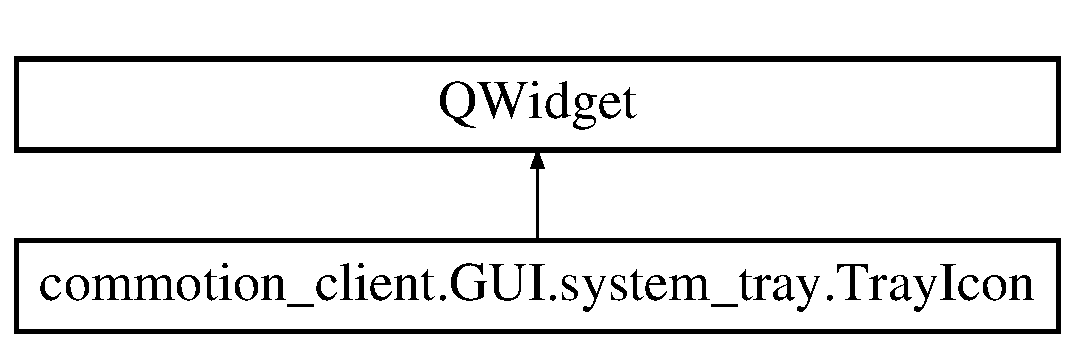
\includegraphics[height=2.000000cm]{classcommotion__client_1_1GUI_1_1system__tray_1_1TrayIcon}
\end{center}
\end{figure}
\subsection*{Public Member Functions}
\begin{DoxyCompactItemize}
\item 
\hypertarget{classcommotion__client_1_1GUI_1_1system__tray_1_1TrayIcon_aca280c4231a261edb8caacd712931840}{def {\bfseries \+\_\+\+\_\+init\+\_\+\+\_\+}}\label{classcommotion__client_1_1GUI_1_1system__tray_1_1TrayIcon_aca280c4231a261edb8caacd712931840}

\item 
def \hyperlink{classcommotion__client_1_1GUI_1_1system__tray_1_1TrayIcon_a31999bfda4008b7395def282e37b4d5c}{tray\+\_\+icon\+Activated}
\end{DoxyCompactItemize}
\subsection*{Public Attributes}
\begin{DoxyCompactItemize}
\item 
\hypertarget{classcommotion__client_1_1GUI_1_1system__tray_1_1TrayIcon_acf0eb7b591dfcf509b0d5eb0d57247dc}{{\bfseries log}}\label{classcommotion__client_1_1GUI_1_1system__tray_1_1TrayIcon_acf0eb7b591dfcf509b0d5eb0d57247dc}

\item 
\hypertarget{classcommotion__client_1_1GUI_1_1system__tray_1_1TrayIcon_a3a048d00c09481b8655b1b6ea357b4e0}{{\bfseries exit}}\label{classcommotion__client_1_1GUI_1_1system__tray_1_1TrayIcon_a3a048d00c09481b8655b1b6ea357b4e0}

\item 
\hypertarget{classcommotion__client_1_1GUI_1_1system__tray_1_1TrayIcon_a1d5c21e34150d0320feeaecce88e42d9}{{\bfseries tray\+\_\+icon}}\label{classcommotion__client_1_1GUI_1_1system__tray_1_1TrayIcon_a1d5c21e34150d0320feeaecce88e42d9}

\end{DoxyCompactItemize}
\subsection*{Static Public Attributes}
\begin{DoxyCompactItemize}
\item 
\hypertarget{classcommotion__client_1_1GUI_1_1system__tray_1_1TrayIcon_a17122b55a08c1aa7d92e9d21e0fac83e}{tuple {\bfseries show\+\_\+main} = Qt\+Core.\+pyqt\+Signal()}\label{classcommotion__client_1_1GUI_1_1system__tray_1_1TrayIcon_a17122b55a08c1aa7d92e9d21e0fac83e}

\end{DoxyCompactItemize}


\subsection{Detailed Description}
\begin{DoxyVerb}The Commotion tray icon. This icon object is the only object that can close the entire application.
\end{DoxyVerb}
 

\subsection{Member Function Documentation}
\hypertarget{classcommotion__client_1_1GUI_1_1system__tray_1_1TrayIcon_a31999bfda4008b7395def282e37b4d5c}{\index{commotion\+\_\+client\+::\+G\+U\+I\+::system\+\_\+tray\+::\+Tray\+Icon@{commotion\+\_\+client\+::\+G\+U\+I\+::system\+\_\+tray\+::\+Tray\+Icon}!tray\+\_\+icon\+Activated@{tray\+\_\+icon\+Activated}}
\index{tray\+\_\+icon\+Activated@{tray\+\_\+icon\+Activated}!commotion\+\_\+client\+::\+G\+U\+I\+::system\+\_\+tray\+::\+Tray\+Icon@{commotion\+\_\+client\+::\+G\+U\+I\+::system\+\_\+tray\+::\+Tray\+Icon}}
\subsubsection[{tray\+\_\+icon\+Activated}]{\setlength{\rightskip}{0pt plus 5cm}def commotion\+\_\+client.\+G\+U\+I.\+system\+\_\+tray.\+Tray\+Icon.\+tray\+\_\+icon\+Activated (
\begin{DoxyParamCaption}
\item[{}]{self, }
\item[{}]{reason}
\end{DoxyParamCaption}
)}}\label{classcommotion__client_1_1GUI_1_1system__tray_1_1TrayIcon_a31999bfda4008b7395def282e37b4d5c}
\begin{DoxyVerb}Defines the tray icon behavior on different types of interactions.
\end{DoxyVerb}
 
\begin{DoxyCode}
30 
31     \textcolor{keyword}{def }\hyperlink{classcommotion__client_1_1GUI_1_1system__tray_1_1TrayIcon_a31999bfda4008b7395def282e37b4d5c}{tray\_iconActivated}(self, reason):
32         \textcolor{stringliteral}{"""}
33 \textcolor{stringliteral}{        Defines the tray icon behavior on different types of interactions.}
34 \textcolor{stringliteral}{        """}
35         \textcolor{keywordflow}{if} reason == QtGui.QSystemTrayIcon.Context:
36             self.tray\_icon.contextMenu().show()
37         \textcolor{keywordflow}{elif} reason == QtGui.QSystemTrayIcon.Trigger:
38             self.show\_main.emit()
\end{DoxyCode}


The documentation for this class was generated from the following file\+:\begin{DoxyCompactItemize}
\item 
commotion\+\_\+client/\+G\+U\+I/system\+\_\+tray.\+py\end{DoxyCompactItemize}

\hypertarget{classcommotion__client_1_1utils_1_1settings_1_1UserSettingsManager}{\section{commotion\-\_\-client.\-utils.\-settings.\-User\-Settings\-Manager Class Reference}
\label{classcommotion__client_1_1utils_1_1settings_1_1UserSettingsManager}\index{commotion\-\_\-client.\-utils.\-settings.\-User\-Settings\-Manager@{commotion\-\_\-client.\-utils.\-settings.\-User\-Settings\-Manager}}
}
Inheritance diagram for commotion\-\_\-client.\-utils.\-settings.\-User\-Settings\-Manager\-:\begin{figure}[H]
\begin{center}
\leavevmode
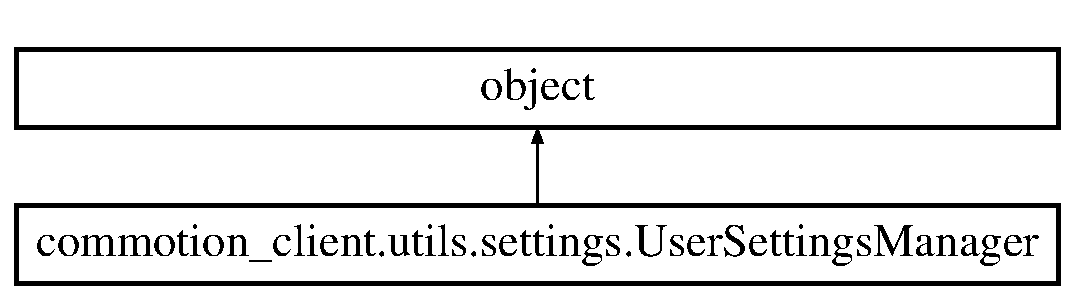
\includegraphics[height=2.000000cm]{classcommotion__client_1_1utils_1_1settings_1_1UserSettingsManager}
\end{center}
\end{figure}
\subsection*{Public Member Functions}
\begin{DoxyCompactItemize}
\item 
def \hyperlink{classcommotion__client_1_1utils_1_1settings_1_1UserSettingsManager_a51d7787bb6bdf12e72b053efc85ae14c}{\-\_\-\-\_\-init\-\_\-\-\_\-}
\item 
def \hyperlink{classcommotion__client_1_1utils_1_1settings_1_1UserSettingsManager_af215df79cfa2281e573a55bb44ca85cd}{save}
\item 
def \hyperlink{classcommotion__client_1_1utils_1_1settings_1_1UserSettingsManager_a8b3fefd45cd8d0747d32267e91d37f07}{load}
\item 
def \hyperlink{classcommotion__client_1_1utils_1_1settings_1_1UserSettingsManager_a6e67fd793c1f0c88a6d28551ba4ef4b3}{get}
\end{DoxyCompactItemize}
\subsection*{Public Attributes}
\begin{DoxyCompactItemize}
\item 
\hypertarget{classcommotion__client_1_1utils_1_1settings_1_1UserSettingsManager_aab010f5c4df9cb099aee2a9644e22058}{{\bfseries settings}}\label{classcommotion__client_1_1utils_1_1settings_1_1UserSettingsManager_aab010f5c4df9cb099aee2a9644e22058}

\end{DoxyCompactItemize}


\subsection{Constructor \& Destructor Documentation}
\hypertarget{classcommotion__client_1_1utils_1_1settings_1_1UserSettingsManager_a51d7787bb6bdf12e72b053efc85ae14c}{\index{commotion\-\_\-client\-::utils\-::settings\-::\-User\-Settings\-Manager@{commotion\-\_\-client\-::utils\-::settings\-::\-User\-Settings\-Manager}!\-\_\-\-\_\-init\-\_\-\-\_\-@{\-\_\-\-\_\-init\-\_\-\-\_\-}}
\index{\-\_\-\-\_\-init\-\_\-\-\_\-@{\-\_\-\-\_\-init\-\_\-\-\_\-}!commotion_client::utils::settings::UserSettingsManager@{commotion\-\_\-client\-::utils\-::settings\-::\-User\-Settings\-Manager}}
\subsubsection[{\-\_\-\-\_\-init\-\_\-\-\_\-}]{\setlength{\rightskip}{0pt plus 5cm}def commotion\-\_\-client.\-utils.\-settings.\-User\-Settings\-Manager.\-\_\-\-\_\-init\-\_\-\-\_\- (
\begin{DoxyParamCaption}
\item[{}]{self}
\end{DoxyParamCaption}
)}}\label{classcommotion__client_1_1utils_1_1settings_1_1UserSettingsManager_a51d7787bb6bdf12e72b053efc85ae14c}
\begin{DoxyVerb}Create a settings object that is tied to a specific scope.
CURRENTLY A DEVELOPMENT STUB!
\end{DoxyVerb}
 

References commotion\-\_\-client.\-G\-U\-I.\-toolbar.\-Tool\-Bar.\-settings, commotion\-\_\-client.\-utils.\-settings.\-User\-Settings\-Manager.\-settings, and commotion\-\_\-client.\-G\-U\-I.\-toolbar\-\_\-builder.\-Tool\-Bar.\-settings.


\begin{DoxyCode}
48 
49     \textcolor{keyword}{def }\hyperlink{classcommotion__client_1_1utils_1_1settings_1_1UserSettingsManager_a51d7787bb6bdf12e72b053efc85ae14c}{\_\_init\_\_}(self):
50         \textcolor{stringliteral}{"""Create a settings object that is tied to a specific scope.}
51 \textcolor{stringliteral}{        CURRENTLY A DEVELOPMENT STUB!}
52 \textcolor{stringliteral}{        """}
53         self.\hyperlink{classcommotion__client_1_1utils_1_1settings_1_1UserSettingsManager_aab010f5c4df9cb099aee2a9644e22058}{settings} = QtCore.QSettings()

\end{DoxyCode}


\subsection{Member Function Documentation}
\hypertarget{classcommotion__client_1_1utils_1_1settings_1_1UserSettingsManager_a6e67fd793c1f0c88a6d28551ba4ef4b3}{\index{commotion\-\_\-client\-::utils\-::settings\-::\-User\-Settings\-Manager@{commotion\-\_\-client\-::utils\-::settings\-::\-User\-Settings\-Manager}!get@{get}}
\index{get@{get}!commotion_client::utils::settings::UserSettingsManager@{commotion\-\_\-client\-::utils\-::settings\-::\-User\-Settings\-Manager}}
\subsubsection[{get}]{\setlength{\rightskip}{0pt plus 5cm}def commotion\-\_\-client.\-utils.\-settings.\-User\-Settings\-Manager.\-get (
\begin{DoxyParamCaption}
\item[{}]{self}
\end{DoxyParamCaption}
)}}\label{classcommotion__client_1_1utils_1_1settings_1_1UserSettingsManager_a6e67fd793c1f0c88a6d28551ba4ef4b3}
\begin{DoxyVerb}CURRENTLY A DEVELOPMENT STUB!\end{DoxyVerb}
 
\begin{DoxyCode}
68 
69     \textcolor{keyword}{def }\hyperlink{classcommotion__client_1_1utils_1_1settings_1_1UserSettingsManager_a6e67fd793c1f0c88a6d28551ba4ef4b3}{get}(self):
70         \textcolor{stringliteral}{"""CURRENTLY A DEVELOPMENT STUB!"""}
71         \textcolor{keywordflow}{return} self.\hyperlink{classcommotion__client_1_1utils_1_1settings_1_1UserSettingsManager_aab010f5c4df9cb099aee2a9644e22058}{settings}
72 
73     
74 
\end{DoxyCode}
\hypertarget{classcommotion__client_1_1utils_1_1settings_1_1UserSettingsManager_a8b3fefd45cd8d0747d32267e91d37f07}{\index{commotion\-\_\-client\-::utils\-::settings\-::\-User\-Settings\-Manager@{commotion\-\_\-client\-::utils\-::settings\-::\-User\-Settings\-Manager}!load@{load}}
\index{load@{load}!commotion_client::utils::settings::UserSettingsManager@{commotion\-\_\-client\-::utils\-::settings\-::\-User\-Settings\-Manager}}
\subsubsection[{load}]{\setlength{\rightskip}{0pt plus 5cm}def commotion\-\_\-client.\-utils.\-settings.\-User\-Settings\-Manager.\-load (
\begin{DoxyParamCaption}
\item[{}]{self}
\end{DoxyParamCaption}
)}}\label{classcommotion__client_1_1utils_1_1settings_1_1UserSettingsManager_a8b3fefd45cd8d0747d32267e91d37f07}
\begin{DoxyVerb}CURRENTLY A DEVELOPMENT STUB!\end{DoxyVerb}
 
\begin{DoxyCode}
59 
60     \textcolor{keyword}{def }\hyperlink{classcommotion__client_1_1utils_1_1settings_1_1UserSettingsManager_a8b3fefd45cd8d0747d32267e91d37f07}{load}(self):
61         \textcolor{stringliteral}{"""CURRENTLY A DEVELOPMENT STUB!"""}
62 
63         \textcolor{comment}{#call pgp to get location of decrypted user file, if any}
64         \textcolor{comment}{#load global settings file.}
65         \textcolor{comment}{# QSettings.setUserIniPath (QString dir)}
66         \textcolor{comment}{#get}
67         \textcolor{keywordflow}{pass}
        
\end{DoxyCode}
\hypertarget{classcommotion__client_1_1utils_1_1settings_1_1UserSettingsManager_af215df79cfa2281e573a55bb44ca85cd}{\index{commotion\-\_\-client\-::utils\-::settings\-::\-User\-Settings\-Manager@{commotion\-\_\-client\-::utils\-::settings\-::\-User\-Settings\-Manager}!save@{save}}
\index{save@{save}!commotion_client::utils::settings::UserSettingsManager@{commotion\-\_\-client\-::utils\-::settings\-::\-User\-Settings\-Manager}}
\subsubsection[{save}]{\setlength{\rightskip}{0pt plus 5cm}def commotion\-\_\-client.\-utils.\-settings.\-User\-Settings\-Manager.\-save (
\begin{DoxyParamCaption}
\item[{}]{self}
\end{DoxyParamCaption}
)}}\label{classcommotion__client_1_1utils_1_1settings_1_1UserSettingsManager_af215df79cfa2281e573a55bb44ca85cd}
\begin{DoxyVerb}CURRENTLY A DEVELOPMENT STUB!\end{DoxyVerb}
 
\begin{DoxyCode}
54 
55     \textcolor{keyword}{def }\hyperlink{classcommotion__client_1_1utils_1_1settings_1_1UserSettingsManager_af215df79cfa2281e573a55bb44ca85cd}{save}(self):
56         \textcolor{stringliteral}{"""CURRENTLY A DEVELOPMENT STUB!"""}
57         \textcolor{comment}{#call PGP to save temporary file to correct encrypted file}
58         \textcolor{keywordflow}{pass}

\end{DoxyCode}


The documentation for this class was generated from the following file\-:\begin{DoxyCompactItemize}
\item 
commotion\-\_\-client/utils/settings.\-py\end{DoxyCompactItemize}

\hypertarget{classcommotion__client_1_1GUI_1_1welcome__page_1_1ViewPort}{\section{commotion\+\_\+client.\+G\+U\+I.\+welcome\+\_\+page.\+View\+Port Class Reference}
\label{classcommotion__client_1_1GUI_1_1welcome__page_1_1ViewPort}\index{commotion\+\_\+client.\+G\+U\+I.\+welcome\+\_\+page.\+View\+Port@{commotion\+\_\+client.\+G\+U\+I.\+welcome\+\_\+page.\+View\+Port}}
}
Inheritance diagram for commotion\+\_\+client.\+G\+U\+I.\+welcome\+\_\+page.\+View\+Port\+:\begin{figure}[H]
\begin{center}
\leavevmode
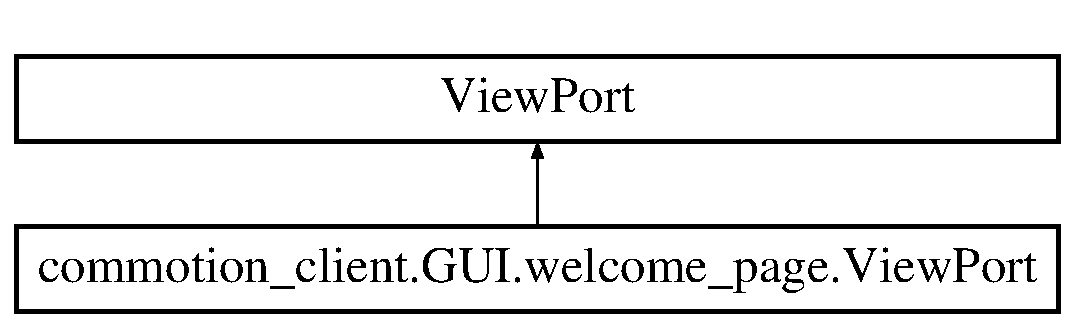
\includegraphics[height=2.000000cm]{classcommotion__client_1_1GUI_1_1welcome__page_1_1ViewPort}
\end{center}
\end{figure}
\subsection*{Public Member Functions}
\begin{DoxyCompactItemize}
\item 
\hypertarget{classcommotion__client_1_1GUI_1_1welcome__page_1_1ViewPort_a816986c73314e7e90ba4105352b819da}{def {\bfseries \+\_\+\+\_\+init\+\_\+\+\_\+}}\label{classcommotion__client_1_1GUI_1_1welcome__page_1_1ViewPort_a816986c73314e7e90ba4105352b819da}

\item 
def \hyperlink{classcommotion__client_1_1GUI_1_1welcome__page_1_1ViewPort_a25e5d500c5e3df779864b936db537770}{is\+\_\+dirty}
\item 
\hypertarget{classcommotion__client_1_1GUI_1_1welcome__page_1_1ViewPort_afdf765ba2c6ae45e8ab8a4172166ac9d}{def {\bfseries clean\+\_\+up}}\label{classcommotion__client_1_1GUI_1_1welcome__page_1_1ViewPort_afdf765ba2c6ae45e8ab8a4172166ac9d}

\end{DoxyCompactItemize}
\subsection*{Public Attributes}
\begin{DoxyCompactItemize}
\item 
\hypertarget{classcommotion__client_1_1GUI_1_1welcome__page_1_1ViewPort_a007c98fbf258770a2e12594c9c083765}{{\bfseries log}}\label{classcommotion__client_1_1GUI_1_1welcome__page_1_1ViewPort_a007c98fbf258770a2e12594c9c083765}

\end{DoxyCompactItemize}
\subsection*{Static Public Attributes}
\begin{DoxyCompactItemize}
\item 
\hypertarget{classcommotion__client_1_1GUI_1_1welcome__page_1_1ViewPort_a38aec86a853649cd2b89b75edafdb97f}{tuple {\bfseries start\+\_\+report\+\_\+collection} = Qt\+Core.\+pyqt\+Signal()}\label{classcommotion__client_1_1GUI_1_1welcome__page_1_1ViewPort_a38aec86a853649cd2b89b75edafdb97f}

\item 
\hypertarget{classcommotion__client_1_1GUI_1_1welcome__page_1_1ViewPort_a6b1fe8a1472a229de25f22ea1f365147}{tuple {\bfseries data\+\_\+report} = Qt\+Core.\+pyqt\+Signal(str, dict)}\label{classcommotion__client_1_1GUI_1_1welcome__page_1_1ViewPort_a6b1fe8a1472a229de25f22ea1f365147}

\item 
\hypertarget{classcommotion__client_1_1GUI_1_1welcome__page_1_1ViewPort_aae1ffc42b8978d237c0cb80374f2c726}{tuple {\bfseries error\+\_\+report} = Qt\+Core.\+pyqt\+Signal(str)}\label{classcommotion__client_1_1GUI_1_1welcome__page_1_1ViewPort_aae1ffc42b8978d237c0cb80374f2c726}

\item 
\hypertarget{classcommotion__client_1_1GUI_1_1welcome__page_1_1ViewPort_a505fd5038731ed162e8b694241157cdb}{tuple {\bfseries on\+\_\+stop} = Qt\+Core.\+pyqt\+Signal()}\label{classcommotion__client_1_1GUI_1_1welcome__page_1_1ViewPort_a505fd5038731ed162e8b694241157cdb}

\end{DoxyCompactItemize}


\subsection{Detailed Description}
\begin{DoxyVerb}\end{DoxyVerb}
 

\subsection{Member Function Documentation}
\hypertarget{classcommotion__client_1_1GUI_1_1welcome__page_1_1ViewPort_a25e5d500c5e3df779864b936db537770}{\index{commotion\+\_\+client\+::\+G\+U\+I\+::welcome\+\_\+page\+::\+View\+Port@{commotion\+\_\+client\+::\+G\+U\+I\+::welcome\+\_\+page\+::\+View\+Port}!is\+\_\+dirty@{is\+\_\+dirty}}
\index{is\+\_\+dirty@{is\+\_\+dirty}!commotion\+\_\+client\+::\+G\+U\+I\+::welcome\+\_\+page\+::\+View\+Port@{commotion\+\_\+client\+::\+G\+U\+I\+::welcome\+\_\+page\+::\+View\+Port}}
\subsubsection[{is\+\_\+dirty}]{\setlength{\rightskip}{0pt plus 5cm}def commotion\+\_\+client.\+G\+U\+I.\+welcome\+\_\+page.\+View\+Port.\+is\+\_\+dirty (
\begin{DoxyParamCaption}
\item[{}]{self}
\end{DoxyParamCaption}
)}}\label{classcommotion__client_1_1GUI_1_1welcome__page_1_1ViewPort_a25e5d500c5e3df779864b936db537770}
\begin{DoxyVerb}The current state of the viewport object \end{DoxyVerb}
 

References commotion\+\_\+client.\+G\+U\+I.\+welcome\+\_\+page.\+View\+Port.\+\_\+dirty, commotion\+\_\+client.\+G\+U\+I.\+main\+\_\+window.\+Main\+Window.\+\_\+dirty, commotion\+\_\+client.\+G\+U\+I.\+toolbar\+\_\+builder.\+Tool\+Bar.\+\_\+dirty, commotion\+\_\+client.\+G\+U\+I.\+toolbar.\+Tool\+Bar.\+\_\+dirty, commotion\+\_\+client.\+G\+U\+I.\+extension\+\_\+toolbar.\+Extension\+Tool\+Bar.\+\_\+dirty, commotion\+\_\+client.\+extensions.\+config\+\_\+editor.\+main.\+View\+Port.\+\_\+dirty, and commotion\+\_\+client.\+G\+U\+I.\+extension\+\_\+toolbar.\+Menu\+Item.\+\_\+dirty.


\begin{DoxyCode}
40 
41     \textcolor{keyword}{def }\hyperlink{classcommotion__client_1_1GUI_1_1welcome__page_1_1ViewPort_a25e5d500c5e3df779864b936db537770}{is\_dirty}(self):
42         \textcolor{stringliteral}{"""The current state of the viewport object """}
43         \textcolor{keywordflow}{return} self.\hyperlink{classcommotion__client_1_1GUI_1_1welcome__page_1_1ViewPort_a785765bd4100c601339cd2172ed99049}{\_dirty}
        
\end{DoxyCode}


The documentation for this class was generated from the following file\+:\begin{DoxyCompactItemize}
\item 
commotion\+\_\+client/\+G\+U\+I/welcome\+\_\+page.\+py\end{DoxyCompactItemize}

\hypertarget{classcommotion__client_1_1extensions_1_1config__editor_1_1main_1_1ViewPort}{\section{commotion\-\_\-client.\-extensions.\-config\-\_\-editor.\-main.\-View\-Port Class Reference}
\label{classcommotion__client_1_1extensions_1_1config__editor_1_1main_1_1ViewPort}\index{commotion\-\_\-client.\-extensions.\-config\-\_\-editor.\-main.\-View\-Port@{commotion\-\_\-client.\-extensions.\-config\-\_\-editor.\-main.\-View\-Port}}
}
Inheritance diagram for commotion\-\_\-client.\-extensions.\-config\-\_\-editor.\-main.\-View\-Port\-:\begin{figure}[H]
\begin{center}
\leavevmode
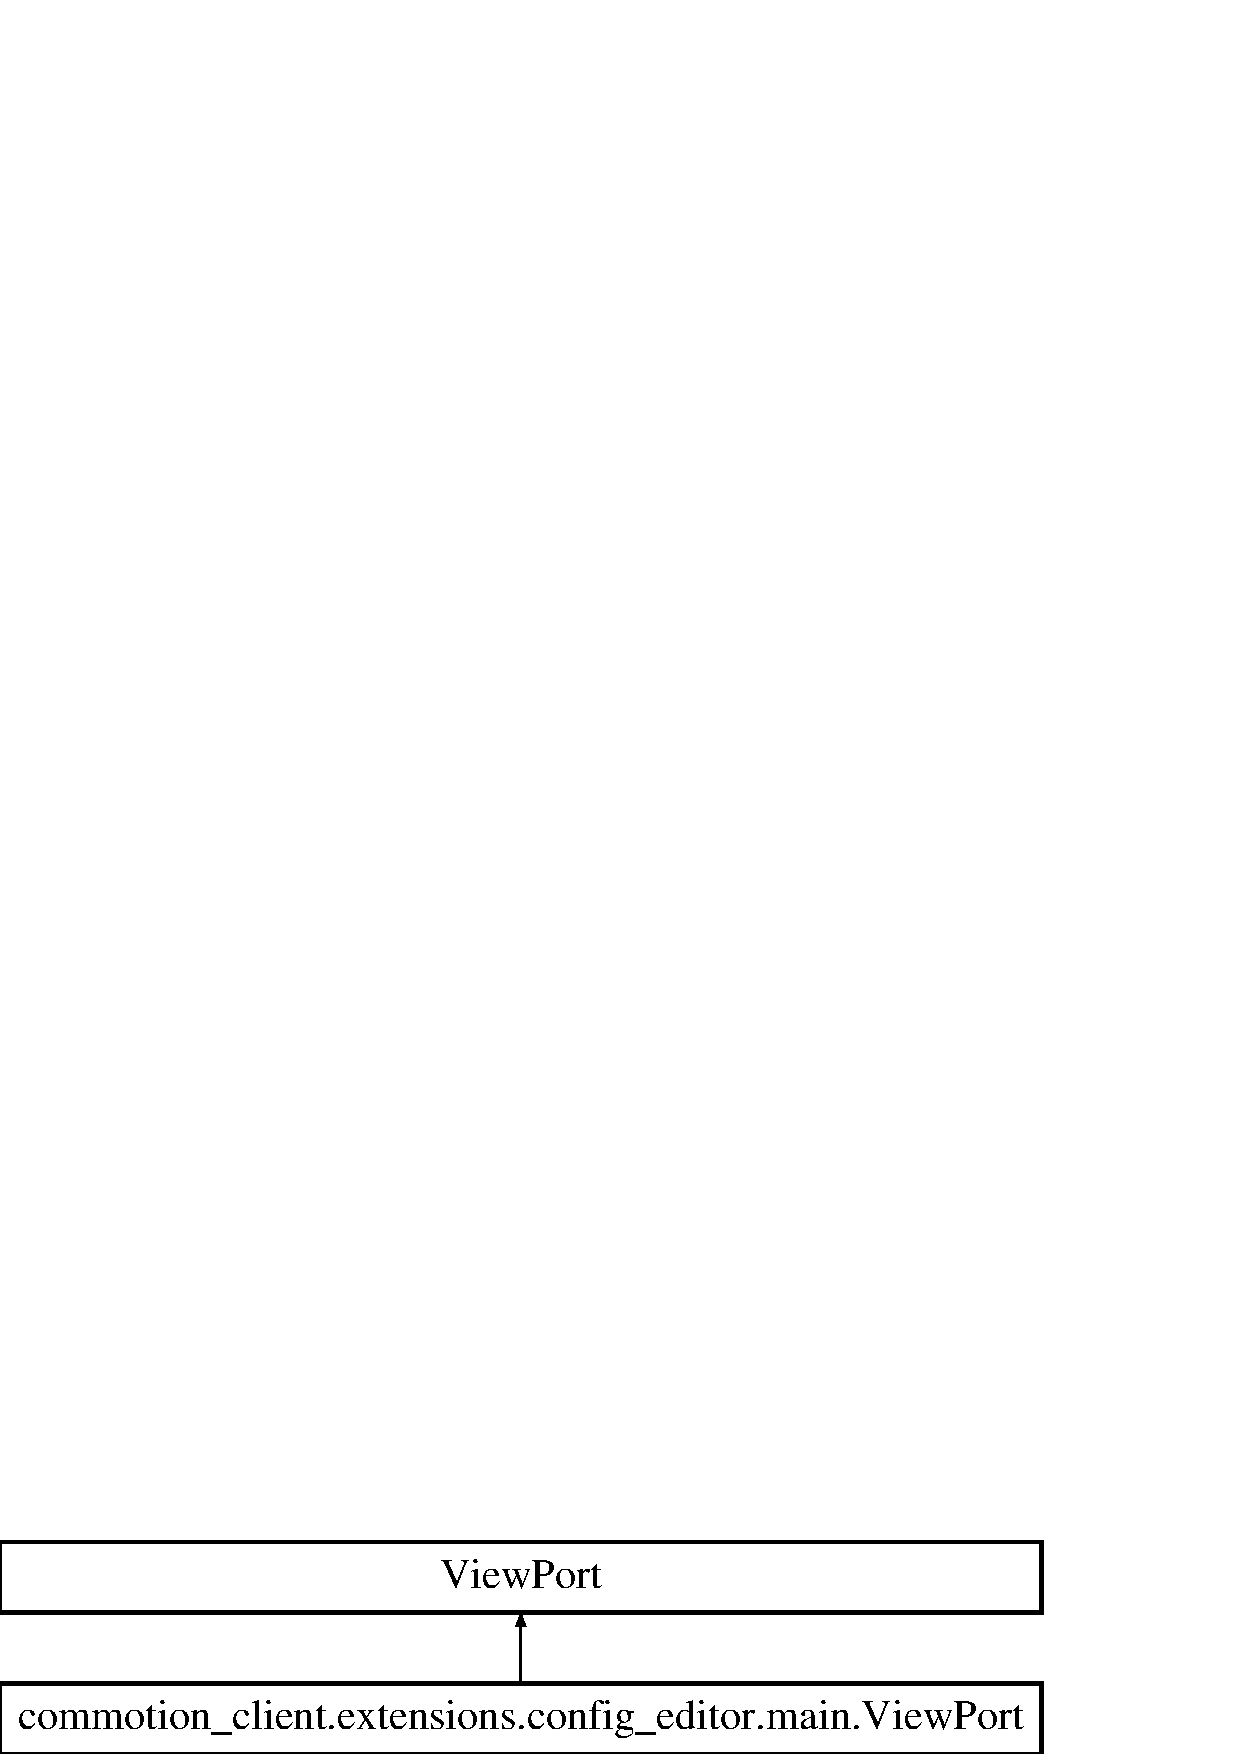
\includegraphics[height=2.000000cm]{classcommotion__client_1_1extensions_1_1config__editor_1_1main_1_1ViewPort}
\end{center}
\end{figure}
\subsection*{Public Member Functions}
\begin{DoxyCompactItemize}
\item 
\hypertarget{classcommotion__client_1_1extensions_1_1config__editor_1_1main_1_1ViewPort_ae9816d12a867e5655be6f810879fb44c}{def {\bfseries \-\_\-\-\_\-init\-\_\-\-\_\-}}\label{classcommotion__client_1_1extensions_1_1config__editor_1_1main_1_1ViewPort_ae9816d12a867e5655be6f810879fb44c}

\item 
def \hyperlink{classcommotion__client_1_1extensions_1_1config__editor_1_1main_1_1ViewPort_a945083e6af1674bdd5cd585fd06a5e60}{is\-\_\-dirty}
\item 
\hypertarget{classcommotion__client_1_1extensions_1_1config__editor_1_1main_1_1ViewPort_a9542b03815bcd39af6208379d4c4f010}{def {\bfseries clean\-\_\-up}}\label{classcommotion__client_1_1extensions_1_1config__editor_1_1main_1_1ViewPort_a9542b03815bcd39af6208379d4c4f010}

\item 
\hypertarget{classcommotion__client_1_1extensions_1_1config__editor_1_1main_1_1ViewPort_a1d04400c68693b3e12de487b21d94349}{def {\bfseries send\-\_\-signal}}\label{classcommotion__client_1_1extensions_1_1config__editor_1_1main_1_1ViewPort_a1d04400c68693b3e12de487b21d94349}

\item 
def \hyperlink{classcommotion__client_1_1extensions_1_1config__editor_1_1main_1_1ViewPort_a09ed3f1dcbee6e902ee8cc00a2e85091}{send\-\_\-error}
\end{DoxyCompactItemize}
\subsection*{Public Attributes}
\begin{DoxyCompactItemize}
\item 
\hypertarget{classcommotion__client_1_1extensions_1_1config__editor_1_1main_1_1ViewPort_a24d4aa0a151b0dca094f962f53936c73}{{\bfseries log}}\label{classcommotion__client_1_1extensions_1_1config__editor_1_1main_1_1ViewPort_a24d4aa0a151b0dca094f962f53936c73}

\item 
\hypertarget{classcommotion__client_1_1extensions_1_1config__editor_1_1main_1_1ViewPort_a83f08f61e1a063c32df35a7e1525951b}{{\bfseries translate}}\label{classcommotion__client_1_1extensions_1_1config__editor_1_1main_1_1ViewPort_a83f08f61e1a063c32df35a7e1525951b}

\end{DoxyCompactItemize}
\subsection*{Static Public Attributes}
\begin{DoxyCompactItemize}
\item 
\hypertarget{classcommotion__client_1_1extensions_1_1config__editor_1_1main_1_1ViewPort_a827b09211733037d237a251a8044ace2}{tuple {\bfseries start\-\_\-report\-\_\-collection} = Qt\-Core.\-pyqt\-Signal()}\label{classcommotion__client_1_1extensions_1_1config__editor_1_1main_1_1ViewPort_a827b09211733037d237a251a8044ace2}

\item 
\hypertarget{classcommotion__client_1_1extensions_1_1config__editor_1_1main_1_1ViewPort_acd90e59ae5c48843e70cacebfb578a29}{tuple {\bfseries data\-\_\-report} = Qt\-Core.\-pyqt\-Signal(str, dict)}\label{classcommotion__client_1_1extensions_1_1config__editor_1_1main_1_1ViewPort_acd90e59ae5c48843e70cacebfb578a29}

\item 
\hypertarget{classcommotion__client_1_1extensions_1_1config__editor_1_1main_1_1ViewPort_a56afd31e2d3659d6d6ac0b29368fe4a1}{tuple {\bfseries error\-\_\-report} = Qt\-Core.\-pyqt\-Signal(str)}\label{classcommotion__client_1_1extensions_1_1config__editor_1_1main_1_1ViewPort_a56afd31e2d3659d6d6ac0b29368fe4a1}

\item 
\hypertarget{classcommotion__client_1_1extensions_1_1config__editor_1_1main_1_1ViewPort_a90efecc3e2b13cfd791b7b5b2a48454a}{tuple {\bfseries clean\-\_\-up} = Qt\-Core.\-pyqt\-Signal()}\label{classcommotion__client_1_1extensions_1_1config__editor_1_1main_1_1ViewPort_a90efecc3e2b13cfd791b7b5b2a48454a}

\item 
\hypertarget{classcommotion__client_1_1extensions_1_1config__editor_1_1main_1_1ViewPort_afc73a9eca8862b7826782c586e43a275}{tuple {\bfseries on\-\_\-stop} = Qt\-Core.\-pyqt\-Signal()}\label{classcommotion__client_1_1extensions_1_1config__editor_1_1main_1_1ViewPort_afc73a9eca8862b7826782c586e43a275}

\end{DoxyCompactItemize}


\subsection{Detailed Description}
\begin{DoxyVerb}pineapple
\end{DoxyVerb}
 

\subsection{Member Function Documentation}
\hypertarget{classcommotion__client_1_1extensions_1_1config__editor_1_1main_1_1ViewPort_a945083e6af1674bdd5cd585fd06a5e60}{\index{commotion\-\_\-client\-::extensions\-::config\-\_\-editor\-::main\-::\-View\-Port@{commotion\-\_\-client\-::extensions\-::config\-\_\-editor\-::main\-::\-View\-Port}!is\-\_\-dirty@{is\-\_\-dirty}}
\index{is\-\_\-dirty@{is\-\_\-dirty}!commotion_client::extensions::config_editor::main::ViewPort@{commotion\-\_\-client\-::extensions\-::config\-\_\-editor\-::main\-::\-View\-Port}}
\subsubsection[{is\-\_\-dirty}]{\setlength{\rightskip}{0pt plus 5cm}def commotion\-\_\-client.\-extensions.\-config\-\_\-editor.\-main.\-View\-Port.\-is\-\_\-dirty (
\begin{DoxyParamCaption}
\item[{}]{self}
\end{DoxyParamCaption}
)}}\label{classcommotion__client_1_1extensions_1_1config__editor_1_1main_1_1ViewPort_a945083e6af1674bdd5cd585fd06a5e60}
\begin{DoxyVerb}The current state of the viewport object \end{DoxyVerb}
 

References commotion\-\_\-client.\-extensions.\-config\-\_\-editor.\-main.\-View\-Port.\-\_\-dirty.



Referenced by commotion\-\_\-client.\-G\-U\-I.\-main\-\_\-window.\-Main\-Window.\-exit\-Event().


\begin{DoxyCode}
49 
50     \textcolor{keyword}{def }\hyperlink{classcommotion__client_1_1extensions_1_1config__editor_1_1main_1_1ViewPort_a945083e6af1674bdd5cd585fd06a5e60}{is\_dirty}(self):
51         \textcolor{stringliteral}{"""The current state of the viewport object """}
52         \textcolor{keywordflow}{return} self.\hyperlink{classcommotion__client_1_1extensions_1_1config__editor_1_1main_1_1ViewPort_a4563ff2ee1897e7348792ef83e49777a}{\_dirty}
        
\end{DoxyCode}
\hypertarget{classcommotion__client_1_1extensions_1_1config__editor_1_1main_1_1ViewPort_a09ed3f1dcbee6e902ee8cc00a2e85091}{\index{commotion\-\_\-client\-::extensions\-::config\-\_\-editor\-::main\-::\-View\-Port@{commotion\-\_\-client\-::extensions\-::config\-\_\-editor\-::main\-::\-View\-Port}!send\-\_\-error@{send\-\_\-error}}
\index{send\-\_\-error@{send\-\_\-error}!commotion_client::extensions::config_editor::main::ViewPort@{commotion\-\_\-client\-::extensions\-::config\-\_\-editor\-::main\-::\-View\-Port}}
\subsubsection[{send\-\_\-error}]{\setlength{\rightskip}{0pt plus 5cm}def commotion\-\_\-client.\-extensions.\-config\-\_\-editor.\-main.\-View\-Port.\-send\-\_\-error (
\begin{DoxyParamCaption}
\item[{}]{self}
\end{DoxyParamCaption}
)}}\label{classcommotion__client_1_1extensions_1_1config__editor_1_1main_1_1ViewPort_a09ed3f1dcbee6e902ee8cc00a2e85091}
\begin{DoxyVerb}HI\end{DoxyVerb}
 
\begin{DoxyCode}
59 
60     \textcolor{keyword}{def }\hyperlink{classcommotion__client_1_1extensions_1_1config__editor_1_1main_1_1ViewPort_a09ed3f1dcbee6e902ee8cc00a2e85091}{send\_error}(self):
61         \textcolor{stringliteral}{"""HI"""}
62         self.error\_report.emit(\textcolor{stringliteral}{"THIS IS AN ERROR MESSAGE!!!"})
63         \textcolor{keywordflow}{pass}
64 
65 

\end{DoxyCode}


The documentation for this class was generated from the following file\-:\begin{DoxyCompactItemize}
\item 
commotion\-\_\-client/extensions/config\-\_\-editor/main.\-py\end{DoxyCompactItemize}

\hypertarget{classcommotion__client_1_1extensions_1_1unit__test__mock_1_1main_1_1ViewPort}{\section{commotion\-\_\-client.\-extensions.\-unit\-\_\-test\-\_\-mock.\-main.\-View\-Port Class Reference}
\label{classcommotion__client_1_1extensions_1_1unit__test__mock_1_1main_1_1ViewPort}\index{commotion\-\_\-client.\-extensions.\-unit\-\_\-test\-\_\-mock.\-main.\-View\-Port@{commotion\-\_\-client.\-extensions.\-unit\-\_\-test\-\_\-mock.\-main.\-View\-Port}}
}
Inheritance diagram for commotion\-\_\-client.\-extensions.\-unit\-\_\-test\-\_\-mock.\-main.\-View\-Port\-:\begin{figure}[H]
\begin{center}
\leavevmode
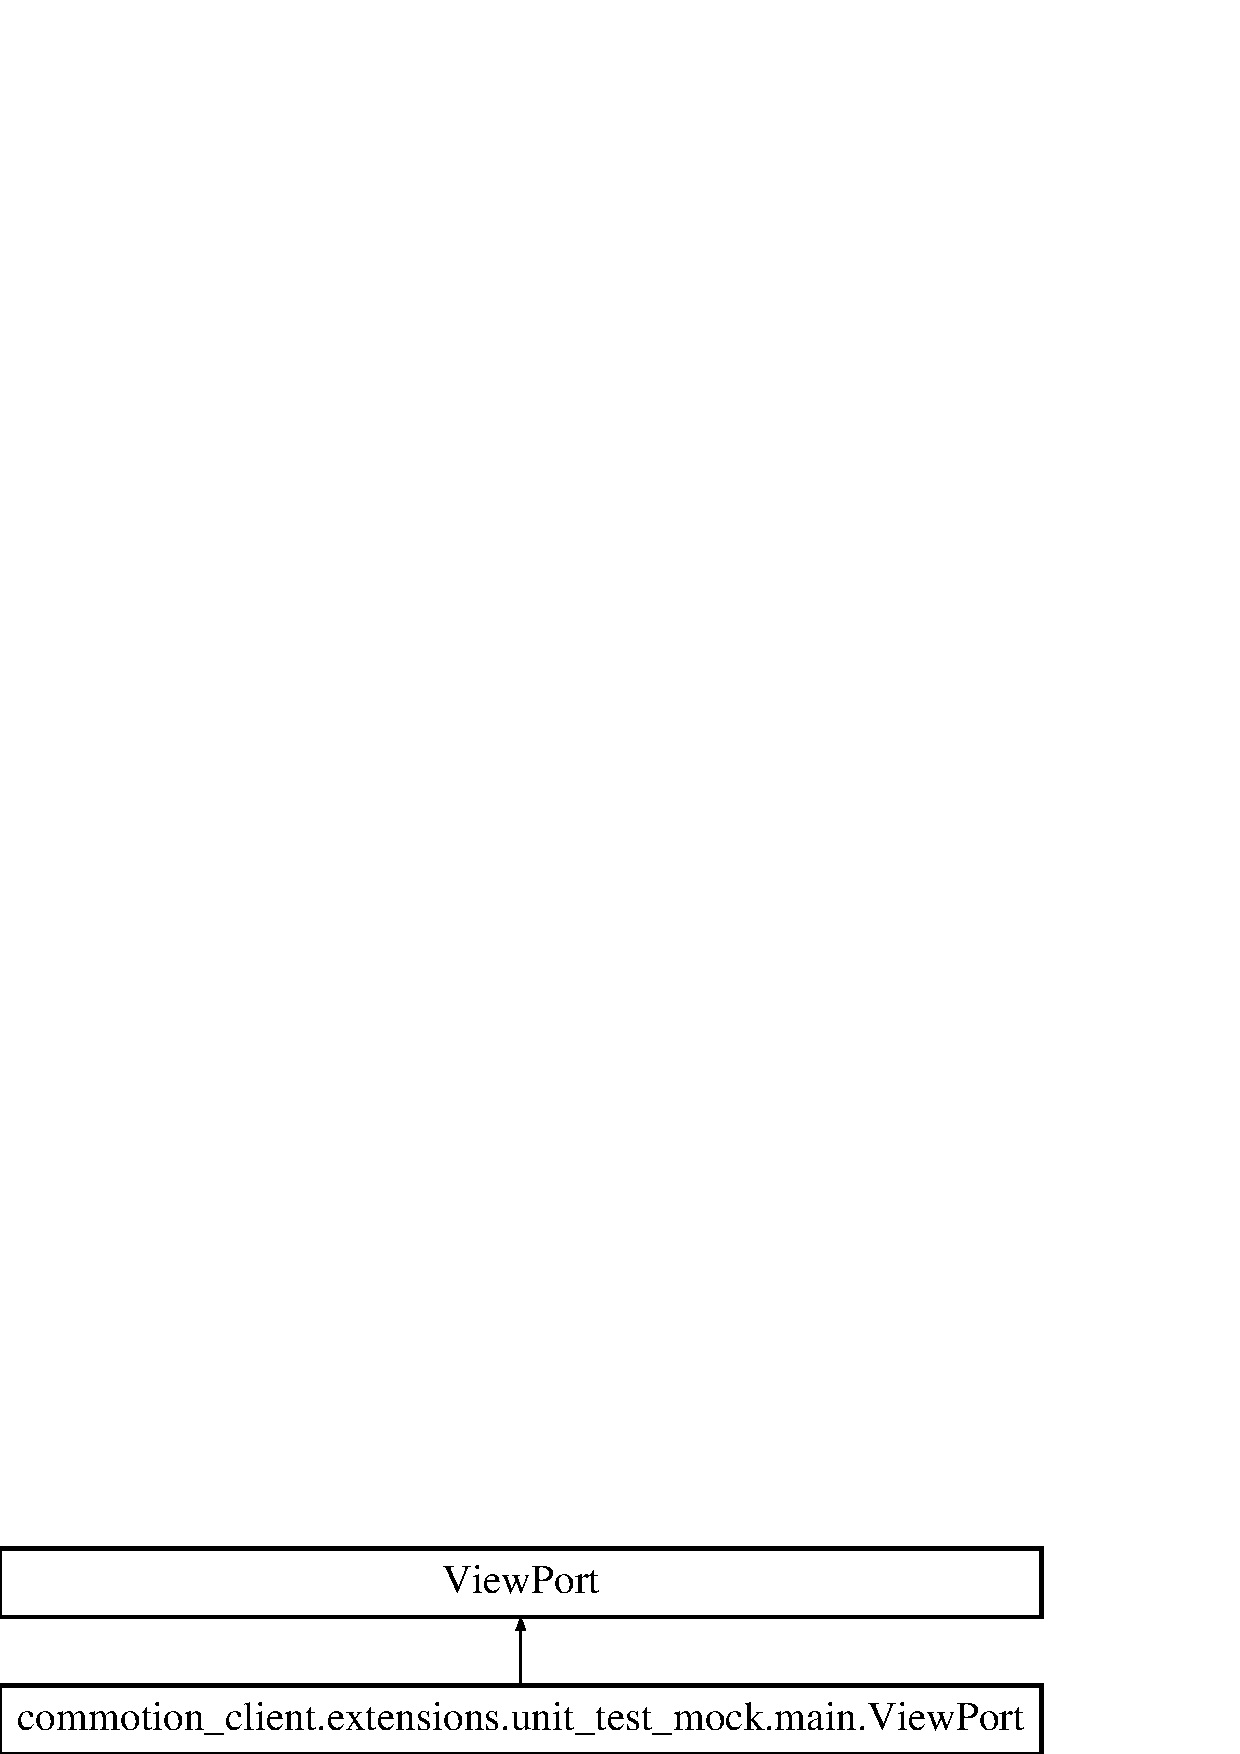
\includegraphics[height=2.000000cm]{classcommotion__client_1_1extensions_1_1unit__test__mock_1_1main_1_1ViewPort}
\end{center}
\end{figure}
\subsection*{Public Member Functions}
\begin{DoxyCompactItemize}
\item 
\hypertarget{classcommotion__client_1_1extensions_1_1unit__test__mock_1_1main_1_1ViewPort_aee1f7a0c54f76a72ad9161a600173b62}{def {\bfseries \-\_\-\-\_\-init\-\_\-\-\_\-}}\label{classcommotion__client_1_1extensions_1_1unit__test__mock_1_1main_1_1ViewPort_aee1f7a0c54f76a72ad9161a600173b62}

\item 
\hypertarget{classcommotion__client_1_1extensions_1_1unit__test__mock_1_1main_1_1ViewPort_a448314ebfe5a2dd40088ba107598e420}{def {\bfseries send\-\_\-signal}}\label{classcommotion__client_1_1extensions_1_1unit__test__mock_1_1main_1_1ViewPort_a448314ebfe5a2dd40088ba107598e420}

\item 
def \hyperlink{classcommotion__client_1_1extensions_1_1unit__test__mock_1_1main_1_1ViewPort_a2f7a09774f0ed12d8588104e76e04027}{send\-\_\-error}
\item 
\hypertarget{classcommotion__client_1_1extensions_1_1unit__test__mock_1_1main_1_1ViewPort_a4889467cc323053dd9a5c2c018ce2843}{def {\bfseries is\-\_\-loaded}}\label{classcommotion__client_1_1extensions_1_1unit__test__mock_1_1main_1_1ViewPort_a4889467cc323053dd9a5c2c018ce2843}

\end{DoxyCompactItemize}
\subsection*{Static Public Attributes}
\begin{DoxyCompactItemize}
\item 
\hypertarget{classcommotion__client_1_1extensions_1_1unit__test__mock_1_1main_1_1ViewPort_a19c8fecac638a284c63499ade7473425}{tuple {\bfseries start\-\_\-report\-\_\-collection} = Qt\-Core.\-pyqt\-Signal()}\label{classcommotion__client_1_1extensions_1_1unit__test__mock_1_1main_1_1ViewPort_a19c8fecac638a284c63499ade7473425}

\item 
\hypertarget{classcommotion__client_1_1extensions_1_1unit__test__mock_1_1main_1_1ViewPort_ac87a5e77b11d3ff2c7daa41e1c07196b}{tuple {\bfseries data\-\_\-report} = Qt\-Core.\-pyqt\-Signal(str, dict)}\label{classcommotion__client_1_1extensions_1_1unit__test__mock_1_1main_1_1ViewPort_ac87a5e77b11d3ff2c7daa41e1c07196b}

\item 
\hypertarget{classcommotion__client_1_1extensions_1_1unit__test__mock_1_1main_1_1ViewPort_a89dad718b1a9f2c8a2755dfd20ba9a69}{tuple {\bfseries error\-\_\-report} = Qt\-Core.\-pyqt\-Signal(str)}\label{classcommotion__client_1_1extensions_1_1unit__test__mock_1_1main_1_1ViewPort_a89dad718b1a9f2c8a2755dfd20ba9a69}

\end{DoxyCompactItemize}


\subsection{Detailed Description}
\begin{DoxyVerb}This is a mock extension and should not be used for ANYTHING user facing!
\end{DoxyVerb}
 

\subsection{Member Function Documentation}
\hypertarget{classcommotion__client_1_1extensions_1_1unit__test__mock_1_1main_1_1ViewPort_a2f7a09774f0ed12d8588104e76e04027}{\index{commotion\-\_\-client\-::extensions\-::unit\-\_\-test\-\_\-mock\-::main\-::\-View\-Port@{commotion\-\_\-client\-::extensions\-::unit\-\_\-test\-\_\-mock\-::main\-::\-View\-Port}!send\-\_\-error@{send\-\_\-error}}
\index{send\-\_\-error@{send\-\_\-error}!commotion_client::extensions::unit_test_mock::main::ViewPort@{commotion\-\_\-client\-::extensions\-::unit\-\_\-test\-\_\-mock\-::main\-::\-View\-Port}}
\subsubsection[{send\-\_\-error}]{\setlength{\rightskip}{0pt plus 5cm}def commotion\-\_\-client.\-extensions.\-unit\-\_\-test\-\_\-mock.\-main.\-View\-Port.\-send\-\_\-error (
\begin{DoxyParamCaption}
\item[{}]{self}
\end{DoxyParamCaption}
)}}\label{classcommotion__client_1_1extensions_1_1unit__test__mock_1_1main_1_1ViewPort_a2f7a09774f0ed12d8588104e76e04027}
\begin{DoxyVerb}HI\end{DoxyVerb}
 
\begin{DoxyCode}
38 
39     \textcolor{keyword}{def }\hyperlink{classcommotion__client_1_1extensions_1_1unit__test__mock_1_1main_1_1ViewPort_a2f7a09774f0ed12d8588104e76e04027}{send\_error}(self):
40         \textcolor{stringliteral}{"""HI"""}
41         self.error\_report.emit(\textcolor{stringliteral}{"THIS IS AN ERROR MESSAGE!!!"})
42         \textcolor{keywordflow}{pass}

\end{DoxyCode}


The documentation for this class was generated from the following file\-:\begin{DoxyCompactItemize}
\item 
commotion\-\_\-client/extensions/unit\-\_\-test\-\_\-mock/main.\-py\end{DoxyCompactItemize}

\hypertarget{classmyMain_1_1viewport}{\section{my\+Main.\+viewport Class Reference}
\label{classmyMain_1_1viewport}\index{my\+Main.\+viewport@{my\+Main.\+viewport}}
}
Inheritance diagram for my\+Main.\+viewport\+:\begin{figure}[H]
\begin{center}
\leavevmode
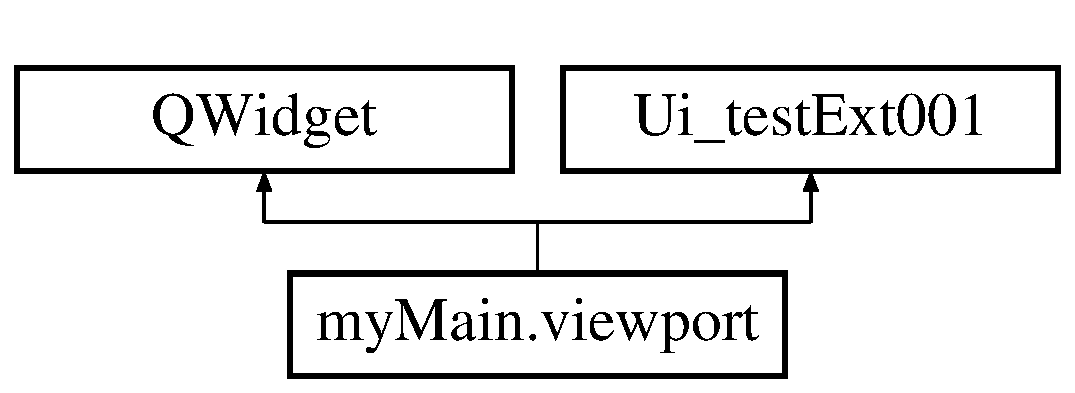
\includegraphics[height=2.000000cm]{classmyMain_1_1viewport}
\end{center}
\end{figure}


The documentation for this class was generated from the following file\+:\begin{DoxyCompactItemize}
\item 
commotion\+\_\+client/tests/extensions/test\+\_\+ext001/my\+Main.\+py\end{DoxyCompactItemize}

\hypertarget{classmain_1_1ViewPort}{\section{main.\+View\+Port Class Reference}
\label{classmain_1_1ViewPort}\index{main.\+View\+Port@{main.\+View\+Port}}
}
Inheritance diagram for main.\+View\+Port\+:\begin{figure}[H]
\begin{center}
\leavevmode
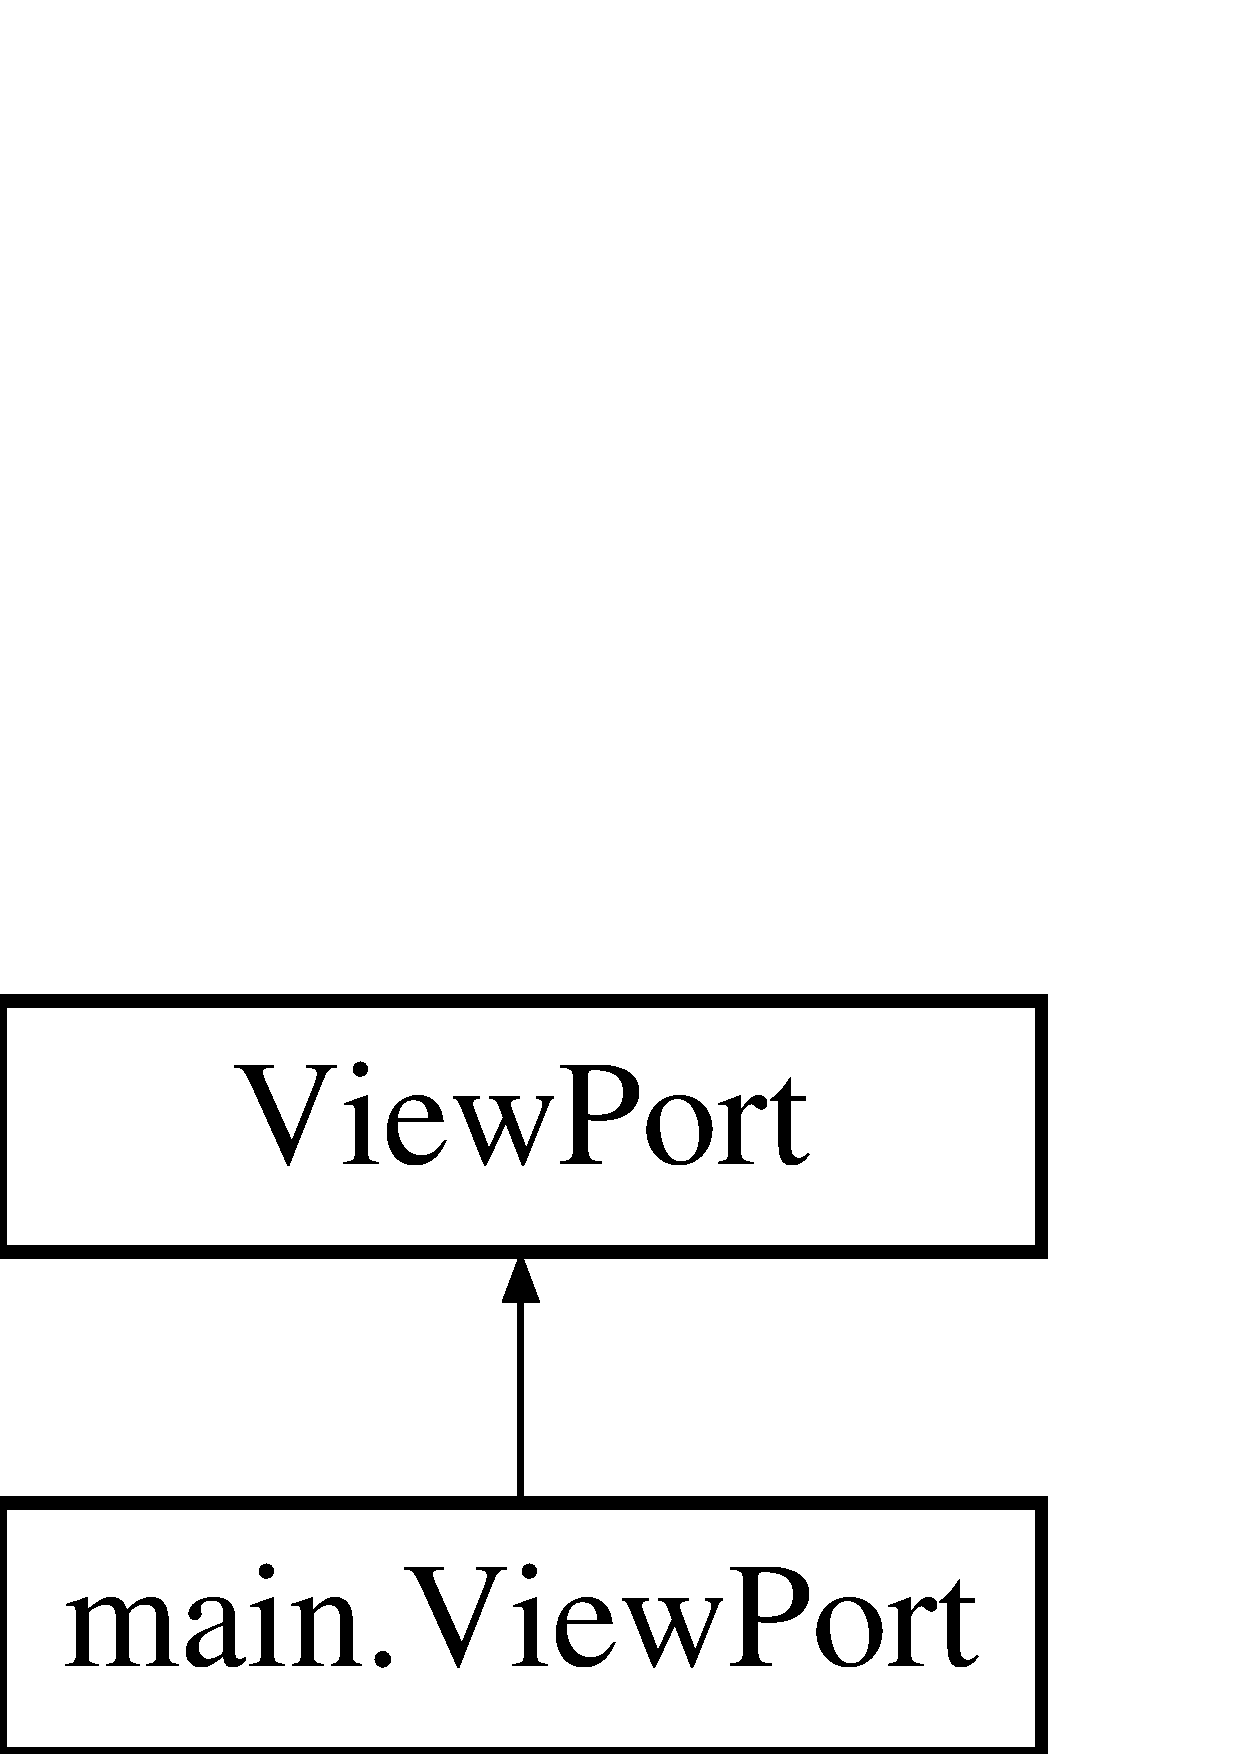
\includegraphics[height=2.000000cm]{classmain_1_1ViewPort}
\end{center}
\end{figure}
\subsection*{Public Member Functions}
\begin{DoxyCompactItemize}
\item 
\hypertarget{classmain_1_1ViewPort_ac5daf01cc84f0883a66c2ec10c33d79c}{def {\bfseries \+\_\+\+\_\+init\+\_\+\+\_\+}}\label{classmain_1_1ViewPort_ac5daf01cc84f0883a66c2ec10c33d79c}

\item 
\hypertarget{classmain_1_1ViewPort_adb11a14a14b2f6e094f714c14b7a58db}{def {\bfseries send\+\_\+signal}}\label{classmain_1_1ViewPort_adb11a14a14b2f6e094f714c14b7a58db}

\item 
\hypertarget{classmain_1_1ViewPort_af36f4fe1b2939d856da39d374ffbf9db}{def {\bfseries send\+\_\+error}}\label{classmain_1_1ViewPort_af36f4fe1b2939d856da39d374ffbf9db}

\item 
def \hyperlink{classmain_1_1ViewPort_a5652106d953c961d92bf96b32e4130b0}{is\+\_\+dirty}
\item 
\hypertarget{classmain_1_1ViewPort_a52a551b8a04099982f77b590289202b3}{def {\bfseries clean\+\_\+up}}\label{classmain_1_1ViewPort_a52a551b8a04099982f77b590289202b3}

\end{DoxyCompactItemize}
\subsection*{Static Public Attributes}
\begin{DoxyCompactItemize}
\item 
\hypertarget{classmain_1_1ViewPort_a082447e10d3654f93bcf4087e83e322f}{tuple {\bfseries start\+\_\+report\+\_\+collection} = Qt\+Core.\+pyqt\+Signal()}\label{classmain_1_1ViewPort_a082447e10d3654f93bcf4087e83e322f}

\item 
\hypertarget{classmain_1_1ViewPort_ade70dbf01fa6abae6d6f9c2f69fe83b9}{tuple {\bfseries data\+\_\+report} = Qt\+Core.\+pyqt\+Signal(str, dict)}\label{classmain_1_1ViewPort_ade70dbf01fa6abae6d6f9c2f69fe83b9}

\item 
\hypertarget{classmain_1_1ViewPort_a8219a346f85e30695bc932ccc0c693fd}{tuple {\bfseries error\+\_\+report} = Qt\+Core.\+pyqt\+Signal(str)}\label{classmain_1_1ViewPort_a8219a346f85e30695bc932ccc0c693fd}

\item 
\hypertarget{classmain_1_1ViewPort_a4eee127d4f68be785562b7e79b237a57}{tuple {\bfseries on\+\_\+stop} = Qt\+Core.\+pyqt\+Signal()}\label{classmain_1_1ViewPort_a4eee127d4f68be785562b7e79b237a57}

\end{DoxyCompactItemize}


\subsection{Detailed Description}
\begin{DoxyVerb}\end{DoxyVerb}
 

\subsection{Member Function Documentation}
\hypertarget{classmain_1_1ViewPort_a5652106d953c961d92bf96b32e4130b0}{\index{main\+::\+View\+Port@{main\+::\+View\+Port}!is\+\_\+dirty@{is\+\_\+dirty}}
\index{is\+\_\+dirty@{is\+\_\+dirty}!main\+::\+View\+Port@{main\+::\+View\+Port}}
\subsubsection[{is\+\_\+dirty}]{\setlength{\rightskip}{0pt plus 5cm}def main.\+View\+Port.\+is\+\_\+dirty (
\begin{DoxyParamCaption}
\item[{}]{self}
\end{DoxyParamCaption}
)}}\label{classmain_1_1ViewPort_a5652106d953c961d92bf96b32e4130b0}
\begin{DoxyVerb}The current state of the viewport object \end{DoxyVerb}
 
\begin{DoxyCode}
48 
49     \textcolor{keyword}{def }\hyperlink{classmain_1_1ViewPort_a5652106d953c961d92bf96b32e4130b0}{is\_dirty}(self):
50         \textcolor{stringliteral}{"""The current state of the viewport object """}
51         \textcolor{keywordflow}{return} self.dirty
        
\end{DoxyCode}


The documentation for this class was generated from the following file\+:\begin{DoxyCompactItemize}
\item 
docs/extensions/extension\+\_\+template/main.\+py\end{DoxyCompactItemize}

%--- End generated contents ---

% Index
\newpage
\phantomsection
\addcontentsline{toc}{chapter}{Index}
\printindex

\end{document}
